%%---------------------------------------------------------------------------------------------------------------------------%%
%% $Id: master-wlarticle.tex 169 2011-11-12 20:27:39Z mip $ #################################################################%%
%%---------------------------------------------------------------------------------------------------------------------------%%
%%
%%
%% Abstract:
%%   LaTeX master file master-wlarticle.tex serves as a template for documents based on the wlarticle document class of the
%% Wegener Center Document Preparation Framework.
%%
%% Details:
%% - Compiling this master file requires a TeX distribution equivalent to TeX Live 2009.
%% - Environment variable settings:
%%   1) $ export TEXMFHOME=<wegc-latex-install-dir>/texmf
%%        # This is only necessary if the Wegener Center Document Preparation Framework is installed to a directory other than
%%        # /usr/local/share or /home/${USER}.
%% - Commands for document generation:
%%   1) $ pdflatex master-wlarticle
%%        # Generate the output document in PDF format by calling pdfTeX in PDF mode. In this case, \documentclass should
%%        # include the ‘pdftex’ output driver option.
%%      $ latex master-wlarticle && dvipdfmx master-wlarticle
%%        # Alternatively, generate the output document in PDF format by calling either TeX or pdfTeX in DVI mode. In this
%%        # case, \documentclass should include the ‘dvipdfmx’ output driver option. If pdfTeX is not installed this command
%%        # replaces the preceding command. If pdfTeX is installed it is an alternative to the preceding command, allowing to
%%        # generate the output document in a way closer to how it would be generated by means of the traditional TeX engine.
%%        # Note that this may imply a significantly smaller PDF file size.
%%   2) $ makeglossaries master-wlarticle
%%        # Generate LaTeX code for formatting the glossary sections. Which index processor is internally called by the
%%        # makeglossaries program depends on the value of the ‘glossaries/processor’ \documentclass option. It can be
%%        # ‘makeindex’ or ‘xindy’.
%%   3) $ bibtex master-wlarticle
%%        # Generate LaTeX code for formatting the bibliography section by means of the bibtex program. In this case,
%%        # \documentclass should set the ‘biblatex/backend’ option to ‘bibtex’.
%%      $ bibtex8 -c <csfile> -W master-wlarticle
%%        # Alternatively, generate LaTeX code for formatting the bibliography section by means of the bibtex8 program. In this
%%        # case, \documentclass should set the ‘biblatex/backend’ option to ‘bibtex8’. <csfile> denotes a BibTeX character set
%%        # and sort definition file such as ascii.csf, latin1.csf or latin9.csf. This should match the encoding of the
%%        # bibliographic database.
%% - Mapping of Unicode characters to LaTeX commands:
%%   - U+2010 --> ‐ --> \hyphen
%%   - U+2011 --> ‑ --> \nbhyphen
%%   - U+2013 --> – --> \textendash
%%   - U+2014 --> — --> \textemdash
%%   - U+2044 --> ⁄ --> \textfractionsolidus
%%   - U+2212 --> − --> \textminus
%%
%% References:
%% - LaTeX 2ε for authors
%%   --> http://tug.ctan.org/tex-archive/macros/latex/doc/usrguide.pdf
%% - The Not So Short Introduction to LaTeX 2ε
%%   --> http://tug.ctan.org/tex-archive/info/lshort/english/lshort.pdf
%% - An essential guide to LaTeX 2ε usage
%%   --> http://tug.ctan.org/tex-archive/info/l2tabu/english/l2tabuen.pdf
%% - KOMA-Script
%%   --> http://tug.ctan.org/tex-archive/macros/latex/contrib/koma-script/scrguide.pdf
%% - Links to the documentation of essential LaTeX packages:
%%   - Multilingual support
%%     --> http://tug.ctan.org/tex-archive/info/babel/babel.pdf
%%   - Professional mathematical formulae
%%     --> http://tug.ctan.org/tex-archive/macros/latex/required/amslatex/math/amsldoc.pdf
%%   - Improved table support
%%     --> http://tug.ctan.org/tex-archive/macros/latex/required/tools/array.pdf
%%   - High-quality tables
%%     --> http://tug.ctan.org/tex-archive/macros/latex/contrib/booktabs/booktabs.pdf
%%   - Multipage tables
%%     --> http://tug.ctan.org/tex-archive/macros/latex/required/tools/longtable.pdf
%%   - Colour support
%%     --> http://tug.ctan.org/tex-archive/macros/latex/contrib/xcolor/xcolor.pdf
%%   - Including external graphics
%%     --> http://tug.ctan.org/tex-archive/macros/latex/required/graphics/grfguide.pdf
%%   - Creating graphics
%%     --> http://tug.ctan.org/tex-archive/graphics/pgf/base/doc/generic/pgf/pgfmanual.pdf
%%   - Numbers and units
%%     --> http://tug.ctan.org/tex-archive/macros/latex/contrib/siunitx/siunitx.pdf
%%   - Chemical formulae
%%     --> http://tug.ctan.org/tex-archive/macros/latex/contrib/mhchem/mhchem.pdf
%%   - Printing source code
%%     --> http://tug.ctan.org/tex-archive/macros/latex/contrib/listings/listings.pdf
%%   - Glossaries
%%     --> http://tug.ctan.org/tex-archive/macros/latex/contrib/glossaries/glossaries-user.pdf
%%   - Bibliographies and citation
%%     --> http://tug.ctan.org/tex-archive/macros/latex/exptl/biblatex/doc/biblatex.pdf
%%   - Hypertext marks
%%     --> http://tug.ctan.org/tex-archive/macros/latex/contrib/hyperref/doc/manual.pdf
%% - Links to the documentation of further LaTeX packages are provided along with the corresponding \RequirePackage statements
%%   in the wltools.sty and wlsetup.sty style files of the Wegener Center Document Preparation Framework.
%%
%% TODO:
%%
%%   None.
%%
%% Author:
%%   Michael H. Pock || MHP || michael.pock@uni-graz.at
%%
%% © Copyright 2008-2011 [ WEGC && IGAM/IP ] / Uni Graz
%%
%%
%%---------------------------------------------------------------------------------------------------------------------------%%
%%###########################################################################################################################%%
%%---------------------------------------------------------------------------------------------------------------------------%%


\documentclass[
  %% output driver (‘pdftex’ when calling pdfLaTeX or ‘dvipdfmx’ when calling LaTeX):
  pdftex,
  %% final or draft document version (‘final’ or ‘draft’):
  final,
  %% web or print document version (‘web’ or ‘print’):
  web,
  %% main document language (‘english’, ‘USenglish’, ‘UKenglish’, ‘ngerman’ or ‘naustrian’):
  UKenglish,
  %% paper size (ISO 216 paper size, North American paper size, ‘portrait’ or ‘landscape’):
  paper=a4,
  %% font size (in pt):
  fontsize=11pt,
  %% DIV factor (‘default’, ‘calc’ or integer >= 4):
  DIV=11,
  %% binding correction (in mm):
  BCOR=0mm,
  %% way of including glossary section headings in the table of contents (‘nottotoc’, ‘totoc’ or ‘totocnumberline’):
  glossaries=totoc,
  %% acronym style (‘default’, ‘dua’, ‘footnote’, ‘smallcaps’, ‘smaller’, ‘description’, ‘description+dua’ or
  %% ‘description+footnote’):
  glossaries/acronymstyle=default,
  %% index processor used along with the glossaries package (‘default’, ‘makeindex’ or ‘xindy’):
  glossaries/processor=makeindex,
  %% bibliography/citation style (‘default’ or a style known to the biblatex package):
  biblatex/style=default,
  %% bibliographic database backend used along with the biblatex package (‘default’, ‘bibtex’ or ‘bibtex8’):
  biblatex/backend=bibtex8,
  %% encoding of the bibliographic database (‘default’, ‘auto’, ‘x-ascii’, ‘x-iso-8859-1’, ‘x-iso-8859-15’ or another
  %% single-byte encoding known to the inputenx package):
  biblatex/bibencoding=x-ascii
]{wlarticle}[2011/11/12]


%%---------------------------------------------------------------------------------------------------------------------------%%
\RequirePackage{acronyms}
\RequirePackage{terms}
\RequirePackage{addresses}
\RequirePackage{commands}
%%---------------------------------------------------------------------------------------------------------------------------%%


%% primary page style of the document (‘empty’, ‘scrplain’ or ‘scrheadings’):
\SetUpPrimaryPageStyle{scrheadings}


%% page style of the title page (‘empty’, ‘scrplain’ or ‘scrheadings’):
\renewcommand*{\titlepagestyle}{%
  scrplain%
}


%%---------------------------------------------------------------------------------------------------------------------------%%


\titlehead{%
  %
}


\subject{%
  %
}


\title{%
  The \wegcLaTeX{} documentation framework: \newline a guide for beginners%
}


\subtitle{%
  %
}


\author{%
  \Name{mip}\thanks{\Address{wegc}}%
}


\date{%
  2013-02-09%
}


\publishers{%
  \Name{wegc}%
}


%%---------------------------------------------------------------------------------------------------------------------------%%


\makeglossaries


\setglossarypreamble[main]{%
  %
}


\setglossarypreamble[acronym]{%
  %
}


\setglossarypreamble[notation]{%
  %
}


\glsunsetall


%%---------------------------------------------------------------------------------------------------------------------------%%


\bibliography{%
%%  exampleBibFile%
}


\defbibnote{refpreamble}{%
  %
}


%%---------------------------------------------------------------------------------------------------------------------------%%


\SetUpHyphenation{%
  hyphenate-like-this donothyphenate%
}


%%---------------------------------------------------------------------------------------------------------------------------%%


\makeatletter


%% NOTE: Here, we can act as class and package authors if we want or need to do so ...


\newcommand*{\singledoc}{%
  \entity{singledoc} %
}

\newcommand*{\multidoc}{%
  \entity{multidoc} %
}


\setkomafont{descriptionlabel}{\normalfont\normalsize}

\def\lst@lettertrue{\let\lst@ifletter\iffalse}

\makeatother


%%---------------------------------------------------------------------------------------------------------------------------%%


\begin{document}


\maketitle


\tableofcontents


\listoffigures


\listoftables


\lstlistoflistings


%% \printglossary[type=notation]


%% \printglossary[type=acronym]


%% \printglossary[type=main]


%%-----------------------------------------%%


%%\nocite{Gorbunov2007a}
%%\nocite{Gorbunov2002a}
%%\nocite{Gorbunov1986}

%%\glsadd{development_team}
%%\glsadd{firlefanzation}

%%\glsadd{urd}
%%\glsadd{add}
%%\glsadd{ddd}
%%\glsadd{sum}
%%\glsadd{atr}


\section[Introduction]{Introduction}
\label{sec:introduction}



\subsection[Scope]{Scope}
\label{subsec:scope}

The intention of this document\footnote{The document in hand is applicable
  to \software{long}{\wegcLaTeX}{0}{9}{5}{200}\p.} is to give new users of
the \wegcLaTeX{} documentation framework a quick introduction on how to use
it in the most efficient way.

Included in this manual are a series of examples on how to create the document layout and how to
use the capabilities of the automatically included \LaTeX{} packages.
No special treatment for typesetting formulas, diagrams or tables is given, as literature
on these topics is readily available.
To a minor extent, it also covers advanced topics mainly relevant to people who want to use \wegcLaTeX{}
within the scope of documentation tasks.

It must be emphasized that it is far beyond the scope of this user guide to address questions about
standard \LaTeX{} concepts. Using \LaTeX{} in a reasonably correct manner is \emph{not} a trivial task.
In fact, it is easy to use it quite wrongly.
It is expected that the reader has a basic understanding on how to create simple \LaTeX{} documents.
So if you are new to \LaTeX{} and/or have never worked in a \LaTeX{} documentation task,
please refer to introductory literature on \LaTeX{}.

At the minimum, you should read %
\textquote[\ctanurl{/tex-archive/info/lshort/english/lshort.pdf}]{%
  The Not So Short Introduction to \LaTeXe%
} %
which provides a very good survey of contemporary \LaTeX{} for both beginners and advanced users.
Nevertheless, it is recommended to study the following documents in some detail:
%
\begin{itemize}
   \item \textquote[]{\LaTeXe{} for authors}
         \footnote{\ctanurl{/tex-archive/macros/latex/doc/usrguide.pdf}}

   \item \textquote[]{An essential guide to \LaTeXe{} usage}
         \footnote{\ctanurl{/tex-archive/info/l2tabu/english/l2tabuen.pdf}}

   \item \textquote[]{\KOMAScript}
         \footnote{\ctanurl{/tex-archive/macros/latex/contrib/koma-script/doc/scrguide.pdf}}

   \item \textquote[]{Math mode}
         \footnote{\url{ftp://ftp.tex.ac.uk/tex-archive/info/math/voss/mathmode/Mathmode.pdf}}

   \item \textquote[]{Using Imported Graphics in \LaTeX{} and pdf\LaTeX}
         \footnote{\ctanurl{/tex-archive/info/epslatex/english/epslatex.pdf}}
\end{itemize}
%
Finally, download and print out the %
\textquote[\url{http://www.stdout.org/~winston/latex/latexsheet.pdf}]{%
  \LaTeXe{} Cheat Sheet%
} %
since this may serve as a handy means for everyday work with \LaTeX.

\wegcLaTeX{} has been developed and is maintained by \Name{mip}. In case of
any questions about \wegcLaTeX{}, please write an email to
\EmailAddress{mip}.



\subsection{Capabilities of \wegcLaTeX{}}
\label{subsec:capabilities}

So, what is the \wegcLaTeX{} documentation framework?
Stated in the most simple way, \wegcLaTeX{} provides an environment for generating documents with a
consistent look and feel. The consistency of the the documents is ensured by providing mechanisms
for consistent usage of common items like names, addresses, email addresses, web addresses, telephone numbers,
abbreviations, acronyms, terms and last but not least, a common and consistent document style for
\singledoc and \multidoc documents.

\smallskip

\singledoc documents have a traditional \LaTeX{} styling, whereas \multidoc
documents are intended for publications that comprise two or more articles,
reports or books, which shall all share a common and consistent layout of
the document front matter, \EG{} title page, distribution list and document
revision history as well as document headings. For a few sample pages of a
\multidoc document, please see \autoref{fig:multiDocTitlepage},
\autoref{fig:multiDocReleaseInfopage},
\autoref{fig:multiDocDistributionList}, \autoref{fig:multiDocChangeRecord}
and \autoref{fig:multiDocHeadings} in
\fullautoref{subsec:usingMultiDocumentTemplates}.

The documents written with \wegcLaTeX{} can be, for example, the
documentation tree associated with a software package, the manual and
handbook set for operating and maintenance procedures of any type of machinery, 
or single documents like \ac{msc} and \ac{phd} theses 
(please see \fullautoref{subsubsec:creatingMasterOrPhdThesis} for an expample),
scientific or technical reports, or papers.

\wegcLaTeX{} provides the means to ensure the consistent layout of the
documents by providing templates for the layout of front matter pages,
title page, distribution list, document revision history, bibliography, as
well as of the lists of figures and tables.

Due to the fact that \wegcLaTeX{} also automatically imports a series of
handy \LaTeX{} packages for the creation and inclusion of external
pictures, diagrams, verbatim text and pretty-printed source code listings,
the user does not need to load any extra packages, but can simply start
writing his or her documentation, taking the provided example documents as
a starting point.

As its name implies, \wegcLaTeX{} is written in the \LaTeX{} document
markup language which is widely used by scientists and other professionals
in both the academic and commercial world.  Distributed under the terms of
the \ac{lppl}, \LaTeX{} is free software.%
\footnote{%
  This statement has sometimes been questioned (\CF{}
  \url{http://en.wikipedia.org/wiki/LPPL}).%
} %
Owing to its platform independence, it can moreover be used in a similar
way on Linux, \ac{mac_os_x}, and Windows machines.

Contemporary \TeX/\LaTeX{} distributions such as \TeXLive{} and \MiKTeX{}
ship with a considerable variety of modules whose capabilities go far
beyond the potentials originally foreseen by the venerable \TeX{}
typesetting system and the \LaTeX{} kernel built on it. In fact, assuming
you are an experienced and sufficiently persistent \LaTeX{} user, you
should nowadays be able to cope with most tasks that might arise while
preparing scientific and/or technical documents.  An incomplete---and, of
course, subjective---list of modules providing the necessary tools for
doing so includes:
%
\begin{labeling}[→]{\KOMAScript{} bundle}
   \item[\KOMAScript{} bundle]%
      modern and highly configurable replacement for the standard \LaTeX{}
      document classes, sophisticated interface for configuring the document
      layout including page style design%
      \footnote{\ctanurl{/tex-archive/macros/latex/contrib/koma-script/doc/scrguide.pdf}}
   \item[\entity{babel} package]%
      multilingual support%
      \footnote{\ctanurl{/tex-archive/macros/latex/required/babel/base/babel.pdf}}
   \item[\entity{url} package]%
      formatting \acp{url}, email addresses, filenames, etc.%
      \footnote{\ctanurl{/tex-archive/macros/latex/contrib/url/url.pdf}}
   \item[\entity{siunitx} package]%
      formatting units of physical quantities%
      \footnote{\ctanurl{/tex-archive/macros/latex/contrib/siunitx/siunitx.pdf}}
   \item[\entity{amsmath} package]%
      high‐quality typesetting of mathematical formulae%
      \footnote{\ctanurl{/tex-archive/macros/latex/required/amslatex/math/amsldoc.pdf}}
   \item[\entity{array} package]%
      replacement for the standard \LaTeX{} tables and arrays%
      \footnote{\ctanurl{/tex-archive/macros/latex/required/tools/array.pdf}}
   \item[\entity{booktabs} package]%
      assistance in producing publication‐quality tables%
      \footnote{\ctanurl{/tex-archive/macros/latex/contrib/booktabs/booktabs.pdf}}
   \item[\entity{longtable} package]%
      creating multipage tables%
      \footnote{\ctanurl{/tex-archive/macros/latex/required/tools/longtable.pdf}}
   \item[\entity{xcolor} package]%
      colour support%
      \footnote{\ctanurl{/tex-archive/macros/latex/contrib/xcolor/xcolor.pdf}}
   \item[\entity{graphicx} package]%
      embedding external graphics given in various formats%
      \footnote{\ctanurl{/tex-archive/macros/latex/required/graphics/grfguide.pdf}}
   \item[\entity{pgf} package]%
      creating graphics%
      \footnote{\ctanurl{/tex-archive/graphics/pgf/base/doc/generic/pgf/pgfmanual.pdf}}
   \item[\entity{mhchem} package]%
      chemical formulae%
      \footnote{\ctanurl{/tex-archive/macros/latex/contrib/mhchem/mhchem.pdf}}
   \item[\entity{listings} package]%
      pretty-printing of source code%
      \footnote{\ctanurl{/tex-archive/macros/latex/contrib/listings/listings.pdf}}
   \item[\entity{glossaries} package]%
      maintaining glossaries, lists of acronyms, indices, etc.\ with
      assistance of the \path{makeindex} program%
      \footnote{\ctanurl{/tex-archive/macros/latex/contrib/glossaries/glossaries-user.pdf}}
   \item[\entity{biblatex} package]%
      maintaining bibliographies based on \BibTeX{} bibliographic database
      files with assistance of the \path{bibtex8} program%
      \footnote{\label{fnote:biblatex}\ctanurl{/tex-archive/macros/latex/exptl/biblatex/doc/biblatex.pdf}}
   \item[\entity{hyperref} package]%
      support for hyperlinks, \ac{pdf} bookmarks, \ac{pdf} document
      information, etc.%
      \footnote{\ctanurl{/tex-archive/macros/latex/contrib/hyperref/doc/manual.pdf}}
   \item[\entity{pdfpages} package]%
      support for inclusion of excerpts from \ac{pdf} documents, etc.%
      \footnote{\ctanurl{/tex-archive/macros/latex/contrib/pdfpages/pdfpages.pdf}}
\end{labeling}


Since 2008, \wegcLaTeX{}, a general purpose document preparation
framework, selects, configures, patches, and extends an adequate
subset of \LaTeX{} modules available from \ac{ctan} according to the
needs of a typical user with scientific and/or technical
background. Not surprisingly, the basis of \wegcLaTeX{} is formed by
just those modules outlined in the preceding list.\footnote{Links to
  the documentation of further \LaTeX{} packages used in \wegcLaTeX{}
  are provided with the corresponding \latexcmd{\RequirePackage{}}
  statements in the \path{wltools.sty} and \path{wlsetup.sty} style
  files of the \wegcLaTeX{} framework} To sum up once more, it can be
said that \wegcLaTeX{} represents a highlevel interface to \LaTeX{}
which should enable its user to write comprehensible, consistent,
reader-friendly, flexible, and easily maintainable scientific and/or
technical documents without being forced to spend much time on looking
into more than the (already comprehensive) fundamentals of the
\LaTeX{} document markup language.



\section{Installation}
\label{sec:installation}


\subsection{Installation instructions}
\label{sec:installationInstructions}

\wegcLaTeX{} is provided in the repository hosted at
\nolinkurl{svn+ssh://wegc203117.uni-graz.at/var/lib/svn/wegc_latex/}.

The prerequisite for using \wegcLaTeX{} is a properly installed full \TeXLive{} 2012 distribution on a Linux workstation,
\IE{} the following packages:
\begin{description}
   % \item for \entity{SuSE 12.2}: \\
   %    \path{texlive}, \path{texlive-latex}, \path{texlive-bin-latex}, \\
   %    \path{texlive-tools}, \path{texlive-bin-tools}, \path{texlive-doc}, and \path{texlive-fonts-extra}
   \item for \entity{Debian 7}: \\
      \path{texlive}, and \path{texlive-full}
\end{description}

It should be noted at this place that \wegcLaTeX{} has not been tested with
\MiKTeX{} yet. Experience shows, however, that, if any, only minor
compatibility issues are to be expected.

For installing \wegcLaTeX{} it is only necessary to copy the \wegcLaTeX{}
\texmf{} tree to the \path{\plh{InstallDir}/texmf} directory, and to set up
to three environment variables. \path{\plh{InstallDir}} denotes the
directory in which \path{./texmf/} itself resides, \EG{} if the user's home
directory is used, to \path{/home/<userId>/texmf/}.

Assuming a workstation using the \entity{bash} command language
interpreter, as a second and final step, setting the three environment
variables can be done by adding the following three lines to the
\path{.bashrc} login script:
%
\begin{CommandLineListing}[style=DefaultFileListing, print=true, gobble=3]
   export TEXMFHOME=<InstallDir>/texmf
   export TEXINPUTS=.:./\{data,figs,tex\}//:../common//:
   export BIBINPUTS=.:../common//:
\end{CommandLineListing}
%
\begin{itemize}
\item The \cmdline{TEXMFHOME} variable defines the \wegcLaTeX{}
  installation directory. In this example, it is set to
  \cmdline{TEXMFHOME=<InstallDir>/texmf}. This is only necessary if
  \wegcLaTeX{} is installed to a directory other than the user's home
  (\path{/home/<userId>/}) or the system's pre-defined path
  (\path{/usr/local/share/}). The \LaTeX{} interpreter searches these two
  paths automatically and will use \wegcLaTeX{}, if found there, also
  without setting the \cmdline{TEXMFHOME} variable.
\item The \cmdline{TEXINPUTS} variable defines the locations where
  \wegcLaTeX{} searches for required packages, data, figures, or \LaTeX{}
  source code files. This is convenient, since any file in the
  \path{./data/}, \path{./figs/}, \path{./tex/} or \path{./common/}
  subdirectories can then be referred to by its basename instead of its
  (absolute or relative) pathname.
\item The \cmdline{BIBINPUTS} variable defines the locations where
  \wegcLaTeX{} searches for \path{*.bib} files.
\end{itemize}
%
\Attention{%
  You should not forget to replace the example directory names with the
  real directory names of your installation. Moreover, you must
  \enquote{source} your \path{~/.bashrc} (\IE{} by entering \cmdline{source
    ~/.bashrc} on the command line) in order for the modified shell
  environment to come into effect. If you already maintain a personal
  \texmf{} tree in a non‐standard location, say \path{~/pubs/texmf}, ensure
  that the above two commands are interpreted \emph{after} the commands
  setting up the shell environment for your personal \texmf{}
  tree. Otherwise, there is some probability that \wegcLaTeX{} will not get
  what it actually expects \ldots
}


\subsection{\wegcLaTeX{} file structure}
\label{subsec:structure}

All files belonging to the \wegcLaTeX{} framework are stored below the
\path{\plh{InstallDir}/texmf/} directory. \path{\plh{InstallDir}} denotes
the directory in which the \path{./texmf/} itself resides.
%
The file structure follows the concept of a so‐called \texmf{} tree. At first
glance, you might deem this structure unnecessarily complicated. As a
matter of fact, it is, however, most adequate, given that the file search
algorithms included in \TeX⁄\LaTeX{} distributions such as \TeXLive{} and
\MiKTeX{} are definitely designed and optimized for \texmf{} trees.

The subsequent list describes the subdirectories of the \wegcLaTeX{} file structure:
\begin{description}
   \item \path{./texmf/bibtex/} \\
      This directory hosts \entity{biblatex}-related files (\EG, style files).
    \item \path{./texmf/doc/} \\
      This directory contains the \wegcLaTeX{} templates for
      \singledoc and \multidoc documents in the \\
      \path{./texmf/doc/latex/wegc-latex/examples/singledoc/}, \\
      \path{./texmf/doc/latex/wegc-latex/examples/multidoc-article/}, \\
      \path{./texmf/doc/latex/wegc-latex/examples/multidoc-report/}, and \\
      \path{./texmf/doc/latex/wegc-latex/examples/multidoc-book/} \\
      directories, as well as the document command and layout template files in the \\
      \path{./texmf/doc/latex/wegc-latex/examples/common/} directory.
   \item \path{./texmf/doc/latex/wegc-latex/examples/singledoc/} \\
      This directory contains the \singledoc article, report and book document templates, \IE,
      \path{master-wlarticle.tex}, \path{master-wlreport.tex}, and \path{master-wlbook.tex}.
   \item \path{./texmf/doc/latex/wegc-latex/examples/multidoc-article/}, \\
         \path{./texmf/doc/latex/wegc-latex/examples/multidoc-report/}, and \\
          \path{./texmf/doc/latex/wegc-latex/examples/multidoc-book/} \\
      These directories contain \multidoc article, report and book document templates, \IE, \\
      \path{./multidoc-article/doc-article.tex}, \\
      \path{./multidoc-book/doc-book.tex}, and \\
      \path{./multidoc-report/doc-report.tex}. \\
      Each of these three subdirectories also contain a
      \path{./data/},
      \path{./figs/} and
      \path{./tex/} subdirectory for storing ASCII, image and \LaTeX{} files used.
   \item \path{./texmf/doc/latex/wegc-latex/examples/common/} \\
      This directory contains the \singledoc and \multidoc document command and layout template files \\
      \path{./common/commands.sty}, \\      
      \path{./common/docstyle.sty}, and \\
      \path{./common/project.sty}. \\
      The acronyms, terms, and address definition files 
      \path{acronyms.sty},
      \path{addresses.sty}, and
      \path{terms.sty} are also to be put into this directory 
      (example only versions of these files are provided in the compressed archive file
      \path{./texmf/doc/latex/wegc-latex/WLG/acronymsAddressesTerms_ExampleDoNotUse.tar.gz}, 
      whereas current and up to date versions of these files should be obtained from the separate 
      repository hosted at
      \nolinkurl{https://wegc203117.uni-graz.at/projects/latex_dbs/browser/arsclisys}.%%
      \footnote{The common acronyms, terms, and address
        definitions are easily accessed by adding its directory path to the
        \path{TEXINPUTS} environment variable.} \\
      %%
      The subdirectory \\
      \path{./common/figs/} \\
      contains the images used with \multidoc document cover pages and document headers.
   \item \path{./texmf/dvipdfmx/} \\
      This directory hosts configuration files for the \entity{DVIPDFMx} package,
      used for translating the \entity{DVI} format to \entity{PDF}.
   \item \path{./texmf/tex/} \\
      This directory hosts, among others, the automatically included \LaTeX{} modules mentioned previously
      and the \wegcLaTeX{} kernel.
   \item \path{./texmf/tex/<TBD>/documentVersionInfo.tex} \\
      This file contains the revision definitions used by \wegcLaTeX{}
      (intended to be updated by a \path{./configure} or \path{./makeDocument} script).
      The revision definition consists of three entities, \IE{} \\
      \cmdline{documentRevision},
      \cmdline{documentMajorVersion}, and
      \cmdline{documentMinorVersion}:
      %
      \begin{CommandLineListing}[print=true, gobble=6]
         \newcommand*{\documentMajorVersion}{5}
         \newcommand*{\documentMinorVersion}{6}
         \newcommand*{\documentRevision}{3072}
      \end{CommandLineListing}
\end{description}

For easier offline reading, the manuals for the \LaTeX{} packages mentioned
in \fullautoref{subsec:scope}, \fullautoref{subsec:capabilities} and
\fullautoref{subsec:extensionsToTheLatexKernel}, together with this manual
(\path{WLG.pdf}), are provided in the directory \path{./LaTeX_PDFs/} as
\ac{pdf} files (at the same directory level as the \wegcLaTeX{} \texmf{}
tree).



\subsection{Generating this document}
\label{subsec:generatingThisDocument}

Assuming the \wegcLaTeX{} framework is already properly installed (see \autoref{sec:installationInstructions}),
for generating this document, proceed as follows:
%%
\begin{enumerate}
   \item
      create a working directory, \EG{} \path{/home/\plh{user}/wlgDocGen/}
   \item
      checkout the latest version of \wegcLaTeX{} to \path{/home/\plh{user}/wlgDocGen/}
   \item
      change to the directory containing the master file \path{WLG.tex}, \IE{} \\
      \cmdline{cd /home/\plh{user}/wlgDocGen/trunk/texmf/doc/latex/wegc-latex/WLG}
   \item
      execute the script \path{makeWLG}, \IE{} \\
      \cmdline{./makeWLG} \\
      for generating the \entity{PDF} file \path{WLG.pdf}
\end{enumerate}


\section{Document generation}
\label{sec:documentGeneration}



\subsection{Commands for document generation}
\label{subsec:commandsForDocumentGeneration}

Assuming that a complete document has been properly written, all the required subdocument \LaTeX{} source code files, data and figure
files are present in the appropriate subdirectories (as described in \autoref{subsec:structure} on \autopageref{subsec:structure}),
and the master \LaTeX{} file is named \path{masterDoc.tex},
then there are 4 steps necessary for generating the print-ready \entity{PDF} document:

\begin{enumerate}

   \item
   \begin{enumerate}
      \item
         \label{item:pdf_mode}
         \cmdline{pdflatex masterDoc} \\
         Generate the output document in \entity{PDF} format by calling
         \pdfTeX{} in \entity{PDF} mode.  In this case,
         \latexcmd{\documentclass} should include the \cmdline{"pdftex"}
         output driver option. This is the recommended (and default) way.
      \item
         \label{item:dvi_mode}
         \cmdline{latex masterDoc && dvipdfmx masterDoc} \\
         Alternatively, generate the output document in \entity{PDF} format by calling either \TeX{} or \pdfTeX{} in \entity{DVI} mode.
         In this case, \latexcmd{\documentclass} should include the \cmdline{"dvipdfmx"} output driver option.
         If \pdfTeX{} is not installed this command replaces the preceding command.
         If \pdfTeX{} is installed it is an alternative to the preceding command, allowing to generate the output document in a way
         closer to how it would be generated by means of the traditional \TeX{} engine.
         Note that this may imply a significantly smaller \entity{PDF} file size.
   \end{enumerate}

   \item
      \label{item:glossaries}
      \cmdline{makeglossaries masterDoc} \\
      Generate \LaTeX{} code for formatting the glossary sections. Which
      index processor is internally called by the makeglossaries program
      depends on the value of the \cmdline{"glossaries/processor"}
      \latexcmd{\documentclass} option.  It can be \cmdline{"makeindex"} or
      \cmdline{"xindy"}. Default is \cmdline{"makeindex"}.

   \item
   \begin{enumerate}
      \item
         \label{item:bibliographyBT8}
         \cmdline{bibtex8 -c <csfile> -W masterDoc} \\
         Generate \LaTeX{} code for formatting the bibliography section by
         means of the \cmdline{bibtex8} program.  In this case,
         \latexcmd{\documentclass} should set the
         \cmdline{"biblatex/backend"} option to \cmdline{"bibtex8"} (this
         is the default). \cmdline{<csfile>} denotes a \BibTeX{} character
         set and sort definition file such as \path{ascii.csf},
         \path{latin1.csf} or \path{latin9.csf}.  This should match the
         encoding of the bibliographic database. Usually you do not need to
         explicitly set the \cmdline{<csfile>}, leaving you with the
         recommended way of formatting the bibliography:\\\cmdline{bibtex8
           -W masterDoc}.
      \item
         \label{item:bibliographyBT}
         \cmdline{bibtex masterDoc} \\
         Generate \LaTeX{} code for formatting the bibliography section by
         means of the bibtex program. In this case,
         \latexcmd{\documentclass} should set the
         \cmdline{"biblatex/backend"} option to \cmdline{"bibtex"}.
   \end{enumerate}

 \item Repeat \autoref{item:pdf_mode} or \autoref{item:dvi_mode} two more
   times to get all references and hyperlinks such as
   \latexcmd{\autoref{}}, \latexcmd{\ac{}} and/or \latexcmd{\textcite{}}
   \ETC{} properly updated.

\end{enumerate}

An example script, which uses as first argument the basename of the
\LaTeX{} master file, is presented in
\autoref{lst:documentGenerationScript}. Please note that during your daily
working routine, it is not necessary to perform all these steps; in most
cases, a simple run of \autoref{item:pdf_mode} will update your
\entity{PDF} most efficiently.

\Attention{%
  The more traditional \path{tex}→\path{dvi}→\path{pdf} document generation
  approach listed under \autoref{item:dvi_mode} does not work well at the
  moment because a few \LaTeX{} modules loaded by \wegcLaTeX{}
  insufficiently support the underlying \entity{dvipdfm} driver.
  Furthermore note that the \entity{glossaries} package does not give any
  indication whether \path{makeindex} must be called at a specific stage of
  document generation to update the \enquote{\glossaryname} and
  \enquote{\acronymname} sections as outlined under
  \autoref{item:glossaries}.  Unfortunately, this circumstance makes the
  implementation of an \emph{intelligent} build system a rather challenging
  task.  Assuming the \enquote{\bibname} section is very large and⁄or
  several secondary reference lists exist, calling \path{bibtex8} is likely
  to result in an error despite specifying the high‐capacity
  \path{-W} switch suggested under
  \autoref{item:bibliographyBT8}. If this happens, resort to the
  \entity{biblatex} package documentation (see \autoref{fnote:biblatex})
  which describes in detail how to maximize the capacity of the
  \path{bibtex8} program at run time.}


\begin{CommandLineListing}[style=DefaultFileListing, print=true, basicstyle={\ttfamily\small}, %
                           basewidth=0.47em, xleftmargin=0pt, gobble=3, %
                           caption={Example script for document generation}, %
                           label=lst:documentGenerationScript]
   #! /bin/bash
   export TEXMFHOME=/home/<userId>/texmf
   export TEXINPUTS=.:./\{data,figs,tex\}//:../common//:
   export BIBINPUTS=.:../common//:

   masterDoc=${1}
   latex=pdflatex
   makeglossaries=makeglossaries
   bibtex='bibtex8 -W'
   rm='/bin/rm -f'
   intermediateFiles='*.acn *.acr *.alg *.aux *.bbl *.blg *-blx.bib *.dvi *.glo *.glg *.gls *.ist *.lof *.log *.lol *.lot *.nlg *.noa *.not *.run.xml *.toc'
   ${rm} ${intermediateFiles} &&
   ${latex} ${masterDoc} &&
   ${makeglossaries} ${masterDoc} &&
   ${bibtex} ${masterDoc} &&
   ${latex} ${masterDoc} &&
   ${makeglossaries} ${masterDoc} &&
   ${latex} ${masterDoc} &&
   ${latex} ${masterDoc} &&
   ${rm} ${intermediateFiles}
\end{CommandLineListing}



\subsection{Global Options for document generation}
\label{subsec:globalOptionsForDocumentGeneration}

In \LaTeX{}, global options are specified in the optional argument of the \latexcmd{\documentclass} command which selects the
document class to be used for a document, usually found at the very beginning of a \LaTeX{} master file.
Global options are not only processed by the document class module, but are also taken into account by subsequently loaded packages.
Thus, they provide the primary means for a \LaTeX{} user to change the overall appearance and other global properties of a document.

An example \latexcmd{\documentclass} command setup for use with \wegcLaTeX{} is given in \fullautoref{lst:documentClassExample} and
a short explanation of the \latexcmd{\documentclass} command values is given in \fullautoref{table:documentClassCommandSettings}.


\begin{landscape}
\begin{CommandLineListing}[style=DefaultFileListing, print=true, basicstyle={\ttfamily\small}, %
                           basewidth=0.47em, xleftmargin=0pt, gobble=3, %
                           caption={Example \latexcmd{\documentclass} command settings in the masterfile}, %
                           label=lst:documentClassExample]
   \documentclass[
     %% output driver ("pdftex" when calling pdfLaTeX or "dvipdfmx" when calling LaTeX):
     pdftex,
     %% final or draft document version ("final" or "draft"):
     draft,
     %% web or print document version ("web" or "print"):
     web,
     %% main document language ("english", "USenglish", "UKenglish", "ngerman" or "naustrian"):
     UKenglish,
     %% paper size (ISO 216 paper size, North American paper size, "portrait" or "landscape"):
     paper=a4,
     %% font size (in pt):
     fontsize=11pt,
     %% DIV factor ("default", "calc" or integer >= 4):
     DIV=11,
     %% binding correction (in mm):
     BCOR=0mm,
     %% way of including glossary section headings in the table of contents ("nottotoc", "totoc" or "totocnumberline"):
     glossaries=totoc,
     %% acronym style ("default", "dua", "footnote", "smallcaps", "smaller", "description", "description+dua" or
     %% "description+footnote"):
     glossaries/acronymstyle=default,
     %% index processor used along with the glossaries package ("default", "makeindex" or "xindy"):
     glossaries/processor=makeindex,
     %% bibliography/citation style ("default" or a style known to the biblatex package):
     biblatex/style=default,
     %% bibliographic database backend used along with the biblatex package ("default", "bibtex" or "bibtex8"):
     biblatex/backend=bibtex8,
     %% encoding of the bibliographic database ("default", "auto", "x-ascii", "x-iso-8859-15" or another
     %% single-byte encoding known to the inputenx package):
     biblatex/bibencoding=x-ascii
   ]{wlarticle}[2011/07/26]
\end{CommandLineListing}
\end{landscape}

\begin{longtable}{l p{6.0cm} p{3.0cm}}
   \caption{Available \latexcmd{\documentclass} command settings in the masterfile} %%
   \label{table:documentClassCommandSettings} \\
   \toprule
   Command item        &  possible values                                                      & example setting \\
   \midrule
   document class      & \entity{wlarticle} | \entity{wlbook} | \entity{wlreport}              & \path{wlreport} \\
   output driver       & \entity{pdftex} | \entity{dvipdfmx}                                   & \path{pdftex} \\
   document version    & \entity{final} | \entity{draft}                                       & \path{final} \\
   document type       & \entity{web} | \entity{print}                                         & \path{print} \\
   document language   & \entity{english} | \entity{UKenglish} | \entity{USenglish} | \newline
                         \entity{ngerman} | \entity{naustrian}                                 & \path{UKenglish} \\
   paper size          & \entity{a4} | \entity{a3}                                             & \path{paper=a4} \\
   font size           & \entity{11pt}                                                         & \path{fontsize=11pt} \\
   \entity{DIV} factor & \entity{default} | \entity{calc} | integer >= 4                       & \path{DIV=11} \\
   binding correction  & binding correction (in mm)                                            & \path{BCOR=5mm} \\
   \bottomrule
\end{longtable}


\subsection{Merging subdocuments}
\label{subsec:mergingSubdocuments}

For merging and joining partial documents or subdocuments to a single
\entity{PDF} document, the \entity{multivalent} tool
(\url{http://multivalent.sourceforge.net/}) is highly recommended.  This
Java based tool requires an up to date Sun-Java installation and can be
downloaded\footnote{The file \path{Multivalent20091027.jar} and an older
  version of this tool (\path{Multivalent20060102.jar}) are stored in the
  directory \path{./LaTeX_PDFs/Multivalent/} for ease of access only.}
%%
from the \entity{multivalent} download page at
\url{http://sourceforge.net/projects/multivalent/files/multivalent/Release20091027/Multivalent20091027.jar/}.\\
For joining two \entity{PDF} files, perform the following steps:
%
\begin{CommandLineListing}[print=true, gobble=0]
   cp Multivalent20060102.jar /usr/local/share/java/
   export CLASSPATH=/usr/local/share/java/*
   java tool.pdf.Merge file1.pdf file2.pdf
\end{CommandLineListing}

Note that for simple applications such as adding one or several cover pages
produced by an external tool in \entity{PDF} format, the \entity{pdfpages}
package included in \wegcLaTeX{} (\autoref{subsec:capabilities}) will be a
more appropriate approach. Please refer to the \entity{pdfpages} manual for
further details.



\section{Commands and environments}
\label{sec:commandsAndEnvironments}


\subsection{Extensions to the \LaTeX{} kernel}
\label{subsec:extensionsToTheLatexKernel}

\begin{description}
\item[\latexcmd{\hyphen}] \enforcenewline%
  Expands to a hyphen with less restrictive hyphenation properties as
  compared to the primitive \enquote{\latexcmd{-}} character. Using
  \latexcmd{\hyphen} within compound words lowers the risk of getting
  overfull horizontal boxes. \\
  \latexcmd{\hyphen} can also be accessed via the Unicode character at code
  point U+2010.

\item[\latexcmd{\nbhyphen}] \enforcenewline%
  Expands to a non\hyphen{}breaking \latexcmd{\hyphen}. \\
  \latexcmd{\nbhyphen} can also be accessed via the Unicode character at
  code point U+2011.

\item[\latexcmd{\textendash}] \enforcenewline%
  Expands to an en-dash, slightly longer than a hyphen. This command is an
  alternative form to using \enquote{\cmdline{--}} in the \LaTeX{} source
  code, which expands to the same en-dash, but with slightly different
  hyphenation properties. The en-dash is used for ranges, \EG{} ``3--7'',
  and to separate name pairs, for example, the text%
  \begin{CommandLineListing}[print=true, xleftmargin=0pt, gobble=4]%
    ``Euler\textendash{}Lagrange, Stefan\textendash{}Sussmann''
  \end{CommandLineListing}
  gives the output: \\
  ``Euler\textendash{}Lagrange, Stefan\textendash{}Sussmann''. \\
  \latexcmd{\textendash} can also be accessed via the Unicode character at
  code point U+2013. For truly compound names (named after one person),
  such as ``Lennard-Jones'', use the simple hyphen. The en-dash is also
  used in German sentences to mark ``parenthetical comments'' (see
  \latexcmd{\textemdash} for the English style to do this), for example:
  \begin{CommandLineListing}[print=true, xleftmargin=0pt, gobble=4]%
    ``Das Wichtigste \textendash{} wenn du es wirklich wissen m\"ochtest
    \textendash{} ist, Bindestriche richtig einzusetzen.''
  \end{CommandLineListing}
  gives the output: \\
  ``Das Wichtigste \textendash{} wenn du es wirklich wissen m\"ochtest
  \textendash{} ist, Bindestriche richtig einzusetzen.'' \\
  Note that in German a space character is used to separate the en-dash
  from the surrounding words.

\item[\latexcmd{\textemdash}] \enforcenewline%
  Expands to an em-dash, slightly longer than a en-dash. This command is an
  alternative form to using \enquote{\cmdline{---}} in the \LaTeX{} source
  code, which expands to the same em-dash, but with slightly different
  hyphenation properties. Use this type of dash for ``parenthetical
  comments''. For example, the text%
  \begin{CommandLineListing}[print=true, xleftmargin=0pt, gobble=4]%
    ``The main thing\textemdash{}if you must know\textemdash{}is to use
    hyphens properly.''
  \end{CommandLineListing}
  gives the output: \\
  ``The main thing\textemdash{}if you must know\textemdash{}is to use hyphens properly.''\\
  \latexcmd{\textemdash} can also be accessed via the Unicode character at
  code point U+2014. For details about how to use the various types of
  dashes, please refer to \EG{} \url{https://en.wikipedia.org/wiki/Dash}.

\item[\latexcmd{\textminus}] \enforcenewline%
  Use this to indicate negative numbers. For example, the text
  \begin{CommandLineListing}[print=true, xleftmargin=0pt, gobble=4]%
    ``\textminus{}128''
  \end{CommandLineListing}
  gives the following output: \\
  `` \textminus{}128''\\
  \latexcmd{\textminus} can also be accessed via the Unicode character at
  code point U+2212.

\item[\latexcmd{\textfractionsolidus}] \enforcenewline%
  Yields a slash with alternative (perhaps more attractive) typeface. The
  hyphenation properties of \latexcmd{\textfractionsolidus} are less
  restrictive than those shown by the standard \LaTeX{} \latexcmd{\slash}
  command and, thus, help avoid overfull horizontal boxes. Using the
  primitive \enquote{\latexcmd{/}} character in ordinary textual contexts
  is in general deprecated. \\
  \latexcmd{\textfractionsolidus} can also be accessed via the Unicode
  character at code point U+2044.

\item[\latexcmd{\backtextfractionsolidus}] \enforcenewline%
  Expands to a backslash with a typeface similar to
  \latexcmd{\textfractionsolidus}.

\item[\latexcmd{\hardbreak}] \enforcenewline%
  Indicates that a line break at the immediately following space is
  undesirable, but still acceptable.

\item[\latexcmd{\enforcenewline}] \enforcenewline%
  Causes a line break, even at positions where this is normally forbidden
  (\EG{} at the start of a paragraph).

\item[\latexcmd{\p\plh{punctuationMark}}] \enforcenewline%
  Enforces the correct spacing after
  \entity{\plh{punctuationMark}}. \latexcmd{\p} supersedes the standard
  \LaTeX{} \latexcmd{\@} command in that it does not destroy kerning.

\item[\latexcmd{\dokerning{\plh{group_1}}{\plh{token}}{\plh{group_2}}}]
  \enforcenewline%
  Restores the kerning between \entity{\plh{group_1}} and
  \entity{\plh{group_2}} lost because of using \entity{\plh{token}}.

\item[\latexcmd{\SetUpHyphenation[\plh{language}]{\plh{hyphenationRules}}}]
  \enforcenewline%
  Lets you specify additional \entity{\plh{hyphenationRules}} for
  \entity{\plh{language}} or, if \entity{\plh{language}} is omitted, for
  the primary language of the document. The \entity{\plh{hyphenationRules}}
  are specified according to the scheme prescribed by the standard \LaTeX{}
  \latexcmd{\hyphenation} command. Note that \latexcmd{\SetUpHyphenation}
  may only be used in the document preamble.

\item[\latexcmd{\fullautoref{\plh{referenceLabel}}}] \enforcenewline%
  This is an interim replacement for the \latexcmd{\vref{}} command from
  the \entity{varioref}
  package\footnote{\ctanurl{/tex-archive/macros/latex/required/tools/varioref.pdf}}
  (which currently produces some undesired side effects). In addition to
  the output of the recommended \latexcmd{\autoref} command, the page
  number of the reference target is printed with \latexcmd{\fullautoref}.

\item[\latexcmd{\software{\plh{short|long}}{\plh{swName}}{\plh{swMajor}}{\plh{swMinor}}{\plh{swMicro}}{swRev}}]
  \enforcenewline%
  Expands to a software version string, \EG{} \\
  \latexcmd{\software{long}{rOPS}{7}{7}{1}{2111}} $\rightarrow$
  \software{long}{rOPS}{7}{7}{1}{2111}, or \newline
  \latexcmd{\software{short}{rOPS}{7}{8}{}{}} $\rightarrow$
  \software{short}{rOPS}{7}{8}{}{} \p.

\item[\latexcmd{\placeholder{\plh{dummyArgument}}}] \enforcenewline%
  Expands to a string indicating a dummy argument, \EG{} \\
  \latexcmd{\placeholder{telephoneNumber}} $\rightarrow$
  \placeholder{telephoneNumber} \p.

\item[\latexcmd{\plh{\plh{dummyArgument}}}] \enforcenewline%
  A shortcut to the previous command \latexcmd{\placeholder{}} is available as \latexcmd{\plh{}}, \EG{} \\
  \latexcmd{\plh{telephoneNumber}} $\rightarrow$ \plh{telephoneNumber} \p.

\item[\latexcmd{\cmdline{\plh{consoleCommandlineString}}}] \enforcenewline%
  Expands to a verbatim, fixed font printed \plh{consoleCommandlineString} as it is commonly encountered at a console commandline, \EG{} \\
  \latexcmd{\cmdline{tar -xzf data_file.tar.gz}} $\rightarrow$ \cmdline{tar
    -xzf data_file.tar.gz} \p.

\item[\latexcmd{\path{\plh{fileOrDirecoryPathName}}}] \enforcenewline%
  Expands to a verbatim, fixed font printed \path{\plh{fileOrDirecoryPathName}}, similar \\
  to \latexcmd{\cmdline}.

\item[\latexcmd{\entity{\plh{textString}}}] \enforcenewline%
  \latexcmd{\entity} is intended to be used for marking a \plh{textString}
  that represents some form of an entity.  For example, the text
  \latexcmd{\entity{Orion}} will be printed as \entity{Orion}\p.

\item[\latexcmd{\supplement{\plh{textStrings}}}] \enforcenewline%
  Expands to the \plh{textStrings} enclosed in square brackets.  For
  example, the text%
  \begin{CommandLineListing}[print=true, xleftmargin=0pt, gobble=4]%
    ``The data \supplement{and the run control files} reside in the
    \path{/data/RAOB/} directory.''
  \end{CommandLineListing}
  gives the output: \\
  ``The data \supplement{and the run control files} reside in the
  \path{/data/RAOB/} directory.''

   % \item[\latexcmd{\insi{\plh{textStrings}}}] \enforcenewline%
   %    Expands to the \plh{textStrings} enclosed in round brackets.
   %    For example \todo{figure out what the \insi{} is intended for}, the text%
   %    \begin{CommandLineListing}[print=true, xleftmargin=0pt, gobble=4]%
   %       ``I do not know what for \insi{and why} the \latexcmd{\insi} is there.''
   %    \end{CommandLineListing}
   %    gives the output: \\
   %       ``I do not know what for \insi{and why} the \latexcmd{\insi} is there.''
   %% TODO: insi is not working as described here. And I do not know how it works...


\item[\latexcmd{\Attention{\plh{blockOfText}}}] \enforcenewline%
  Expands to a boldface string reading \textbf{Attention:} followed by \plh{blockOfText}. \\
  For example, the text%
  \begin{CommandLineListing}[print=true, xleftmargin=0pt, gobble=4]%
    \Attention{%
      Please note that keeping food near any terminal device
      might cause unpredictable results during program execution!
    }
  \end{CommandLineListing}
  gives the output: \\
  \Attention{%
    Please note that keeping food near any terminal device
    might cause unpredictable results during program execution!
  }

\item[\latexcmd{\highlight{\plh{blockOfText}}}] \enforcenewline%
  Expands to a yellow highlighted \plh{blockOfText}, independent of the document version (\entity{final} | \entity{draft}).
  For example, the text%
  \begin{CommandLineListing}[print=true, xleftmargin=0pt, gobble=4]%
    \highlight{The output values are still unexpected!}
  \end{CommandLineListing}
  gives the output: \\
  \highlight{The output values are still unexpected!}

  \Attention{%
    The \latexcmd{\highlight} command does not automatically produce any linebreaks
    and it is not sensitive to \latexcmd{\enforcenewline} and \latexcmd{\newline} commands.
    As a matter of fact, it can not be used to highlight more than one line of text.
  }

\item[\latexcmd{\todo{\plh{blockOfText}}}] \enforcenewline%
  With a document version \entity{draft}, it expands to a sequentially
  numbered red text \emph{TODO} at the paper margin near the location
  where the \latexcmd{\todo} appears, and a list of \entity{TODOs},
  sequentially numbered, with a page indicator and the associated
  \plh{blockOfText} at the end of the document. With a document version \entity{final}, the \latexcmd{\todo} is completely ignored. \\
  An example \latexcmd{\todo} command could read:%
  \begin{CommandLineListing}[print=true, xleftmargin=0pt, gobble=4]%
    \todo{Table values need to be updated for the latest measurements!}
  \end{CommandLineListing}

\item[\latexcmd{\No{}}, \latexcmd{\CF{}}, \latexcmd{\EG{}}, \latexcmd{\ETC{}}, and \latexcmd{\IE{}}] \enforcenewline%
  \latexcmd{\No{}}, \latexcmd{\CF{}}, \latexcmd{\EG{}}, \latexcmd{\ETC{}}, and \latexcmd{\IE{}}
  are expanded to conveniently formatted strings, \EG{} \newline
  the \latexcmd{\No{}} 4711 is magic           ~ $\rightarrow$ ~  the \No{} 4711 is magic \newline
  is true, \latexcmd{\CF{}} the letter of      ~ $\rightarrow$ ~  is true, \CF{} the letter of \newline
  is false, \latexcmd{\EG{}} in the case of    ~ $\rightarrow$ ~  is false, \EG{} in the case of \newline
  mist, smoke, \latexcmd{\ETC{}} in air.       ~ $\rightarrow$ ~  mist, smoke, \ETC{} in air. \newline
  is always the case, \latexcmd{\IE{}} true.   ~ $\rightarrow$ ~  is always the case, \IE{} true.

\item[\latexcmd{\pdfTeX{}}, \latexcmd{\pdfLaTeX{}}, \latexcmd{\TeXLive{}}, \latexcmd{\MiKTeX{}}, \latexcmd{\AUCTeX{}}, and \latexcmd{\texmf{}}] \enforcenewline%
  \latexcmd{\pdfTeX{}}, \latexcmd{\pdfLaTeX{}}, \latexcmd{\TeXLive{}}, \latexcmd{\MiKTeX{}}, \latexcmd{\AUCTeX{}}, and \latexcmd{\texmf{}}
  are expanded to conveniently formatted strings, \EG{} \newline
  \latexcmd{\pdfTeX{}}, \latexcmd{\pdfLaTeX{}}, \latexcmd{\TeXLive{}}, \latexcmd{\MiKTeX{}}, \latexcmd{\AUCTeX{}}, and \latexcmd{\texmf{}}
  ~ $\rightarrow$ ~
  \pdfTeX{}, \pdfLaTeX{}, \TeXLive{}, \MiKTeX{}, \AUCTeX{}, and \texmf{}

\item[\latexcmd{\wegcLaTeX{}}] \enforcenewline%
  \latexcmd{\wegcLaTeX{}} is expanded to conveniently formatted string, \EG{} \newline
  the \latexcmd{\wegcLaTeX{}} framework  ~ $\rightarrow$ ~ the \wegcLaTeX{} framework
\end{description}


\subsection[Address book database]{Using the address book database}
\label{subsec:usingTheAddressBookDatabase}

As already mentioned in \autoref{subsec:capabilities}, \wegcLaTeX{}
provides a handy mechanism for consistent usage of names, addresses, email
addresses, web addresses, telephone numbers, and fax numbers via an
extension to the \KOMAScript{} bundle.

The address book entries can be used for referring to real persons as well
as to an organization or an institute.  In the latter case, the field which
stores the \enquote{last name} should be (by convention) left empty.
Address book entries are to be stored in a file named \path{addresses.sty}
in a directory which is included in the search path defined by the
\cmdline{TEXINPUTS} environment variable.

For the addresses to be expanded in a document, the command
\latexcmd{\RequirePackage{addresses}} has to be added directly behind the
\latexcmd{\documentclass} directive in the \LaTeX{} master file.

The address book entry for a fictive person ``\Name{kmf}'' could be
configured by adding the following lines to the \path{addresses.sty} file:
%
\begin{CommandLineListing}[style=DefaultFileListing, print=true, xleftmargin=0pt, gobble=3, %
                           caption={Example \latexcmd{\newaddressbookentry} address book entry in \latexcmd{addresses.sty}}, %
                           label=lst:addressBookExample]
   \newaddressbookentry{kmf}{%
     Karo%
   }{%
     K.%
   }{%
     Musterfrau%
   }{%
     Berggasse 37, A-1234 Lanenberg%
   }{%
     \tel{43}{123}{380}{8400}{}%
   }{%
     \fax{43}{123}{380}{8400}{36}%
   }{%
     \email{karo.musterfrau@gmx.at}%
   }{%
     \url{http://www.musterfrau.at}%
   }
\end{CommandLineListing}

The eight fields for the address book entry of a person, identified by its
shortcut \entity{personId}, \IE{}
\latexcmd{\newaddressbookentry{\plh{personId}}{\plh{field_1}}{\plh{field_2}} ... {\plh{field_8}}}, \\
are defined as described in \autoref{table:addressBookDefinition} and may
be used or extracted as indicated in
\autoref{table:addressBookExample}. The full name of \plh{personId} is
accessed via the command \latexcmd{\Name{\plh{personId}}}, resulting in an
output of ``\Name{kmf}'', and the short name of \plh{personId} is accessed
via the command \latexcmd{\ShortName{\plh{personId}}}, resulting in an
output of ``\ShortName{kmf}''.

Please note that the \latexcmd{\newaddressbookentry} field definitions make
use of the \LaTeX{} commands \latexcmd{\tel{}}, \latexcmd{\fax{}},
\latexcmd{\email{}}, and \latexcmd{\url{}} for properly formatting the
fields.\footnote{If it is desired to suppress the hyperlinking of an email
  or web addresses, the \LaTeX{} commands \latexcmd{\nolinkemail{}} and
  \latexcmd{\nolinkurl{}} can be used instead of \latexcmd{\email{}} and
  \latexcmd{\url{}}.}


\begin{longtable}{l p{5.0cm} p{4.0cm}}
  \caption{Using the \latexcmd{\newaddressbookentry} entries in \latexcmd{addresses.sty}} %%
   \label{table:addressBookExample} \\
   \toprule
   Item              & Example setting/access                        &  Example output    \\
   \midrule
   first name        & \path{Karo}                                   &                    \\
   abbr.\ first name & \path{K.}                                     &                    \\
   last name         & \path{Musterfrau}                             &                    \\
   address           & \path{Berggasse 37, A-1234 Lanenberg}         &                    \\
   tel.\ number      & \latexcmd{\tel{43}{123}{380}{8400}{}}         &                    \\
   fax number        & \latexcmd{\fax{43}{123}{380}{8400}{36}}       &                    \\
   email address     & \latexcmd{\email{karo.musterfrau@gmx.at}}     &                    \\
   web address       & \latexcmd{\url{http://www.musterfrau.at}}     &                    \\
   \midrule
   name              & \latexcmd{\Name{kmf}}                         & \Name{kmf}         \\
   short name        & \latexcmd{\ShortName{kmf}}                    & \ShortName{kmf}    \\
   address           & \latexcmd{\Address{kmf}}                      & \Address{kmf}      \\
   telephone number  & \latexcmd{\Telephone{kmf}}                    & \Telephone{kmf}    \\
   fax number        & \latexcmd{\Fax{kmf}}                          & \Fax{kmf}          \\
   email address     & \latexcmd{\EmailAddress{kmf}}                 & \EmailAddress{kmf} \\
   web address       & \latexcmd{\WebAddress{kmf}}                   & \WebAddress{kmf}   \\
   \bottomrule
\end{longtable}


\begin{longtable}{l p{5.2cm} p{5.0cm}}
  \caption{Definition of \latexcmd{\newaddressbookentry} entries in \latexcmd{addresses.sty}} %%
   \label{table:addressBookDefinition} \\
   \toprule
   Field                  & Content                                     & Command for access                 \\
   \midrule
   \entity{\plh{field_1}} & first name of \entity{\plh{personId}}       &                                    \\
   \entity{\plh{field_2}} & abbr.\ first name of \entity{\plh{personId}}&                                    \\
   \entity{\plh{field_3}} & last name of \entity{\plh{personId}}        &                                    \\
   \entity{\plh{field_4}} & address of \entity{\plh{personId}}          & \latexcmd{\Address{personId}}      \\
   \entity{\plh{field_5}} & tel.\ number of \entity{\plh{personId}}     & \latexcmd{\Telephone{personId}}    \\
   \entity{\plh{field_6}} & fax number of \entity{\plh{personId}}       & \latexcmd{\Fax{personId}}          \\
   \entity{\plh{field_7}} & email address of \entity{\plh{personId}}    & \latexcmd{\EmailAddress{personId}} \\
   \entity{\plh{field_8}} & web address of \entity{\plh{personId}}      & \latexcmd{\WebAddress{personId}}   \\
   \bottomrule
\end{longtable}


\subsection[Acronym database]{Using the acronym database}
\label{subsec:UsingTheAcronymDatabase}


\wegcLaTeX{} includes the \entity{glossaries} package, which provides a
handy mechanism for consistent usage of names and their acronyms.

Acronym entries are to be stored in a file named \path{acronyms.sty} in a
directory which is included in the search path defined by the
\cmdline{TEXINPUTS} environment variable.

The command \latexcmd{\RequirePackage{acronyms}} has to be added to the
\LaTeX{} master file directly behind the \latexcmd{\documentclass} command
to make the acronym definitions available in the document. In addition, the
command \latexcmd{\printglossary[type=acronym]} has to be included between
the \latexcmd{\begin{document}} and \latexcmd{\end{document}} directives.
Acronyms used in the main body of the document are then added to the
acronym list.  If one or more additional acronyms should be included in the
acronym list, irrespective of having been used or not, they can be added
via \latexcmd{\glsadd{\plh{acronymId}}} commands in the main body of the
document.

The acronym for a fictive company ``\acf{tmc}'' could be defined by adding
the following lines to the \path{acronyms.sty} file:
%
\begin{CommandLineListing}[style=DefaultFileListing, print=true, xleftmargin=0pt, gobble=3, %
                           caption={Example \latexcmd{\newacronym} entry in \latexcmd{acronyms.sty}}, %
                           label=lst:addressBookExample]
   \newacronym[description={%
     The Muppet Company \textemdash{} a respected and trusted supplier of evocative learning systems}]{tmc}{TMC}{%
     The Muppet Company\p, Inc\p.%
   }
\end{CommandLineListing}


The four fields for an acronym entry,
identified by its shortcut \entity{acronymId}, \IE{} \\
\latexcmd{\newacronym[description={\plh{field_1}}]{\plh{field_2}}{\plh{field_3}}{\plh{field_4}}}, \\
are defined as described in \autoref{table:acronymDefinition}.
%
\begin{table}%[tb!]
  \caption{Definition of \latexcmd{\newacronym} entries in \latexcmd{acronyms.sty}} %%
  \label{table:acronymDefinition}
  \begin{tabular}{l p{8.5cm} l}
   \toprule
   Field                  & Content                                             & Command                   \\
   \midrule
   \entity{\plh{field_1}} & description of acronym \entity{\plh{acronymId}} (optional).
                            This text, together with the acronym itself, is
                            used in the acronym list. If the description
                            field (together with the
                            \entity{\plh{description}} keyword)
                            is left out, \entity{\plh{field_4}} is
                            used instead.                                       &                            \\
   \entity{\plh{field_2}} & acronym identifier, \IE{} \entity{\plh{acronymId}}  &                            \\
   \entity{\plh{field_3}} & acronym used for \entity{\plh{acronymId}}           & \latexcmd{\acs{acronymId}} \\
   \entity{\plh{field_4}} & explicit text of acronym \entity{\plh{acronymId}}   & \latexcmd{\acl{acronymId}} \\
   \bottomrule
 \end{tabular}
\end{table}
%
The commands for using the acronyms are listed in the following
(\autoref{table:acronymcommands}):
\begin{longtable}{m{0.25\linewidth}m{0.69\linewidth}}
  \caption{List of acronym commands}
  \label{table:acronymcommands} \\
  \toprule
  \latexcmd{\ac{acronymId}} & Prints the acronym plus the explicit text of
  acronym when used for the first time; any further use of \latexcmd{\ac{}}
  will no longer generate the acronym plus the explicit text of the
  acronym, but the acronym only\textemdash{}unless it is reset with a
  \latexcmd{\glsreset{}} or \latexcmd{\glsresetall} command. This is the
  recommended command to use, since it will automatically guarantee the
  consistent usage of acronyms within the document. \\
  \midrule
  \latexcmd{\acs{acronymId}} & Prints the acronym only (short form). \\
  \midrule
  \latexcmd{\acl{acronymId}} & Prints the explicit text of acronym (long
  form). \\
  \midrule
  \latexcmd{\acf{acronymId}} & Prints the acronym plus the explicit text
  of acronym (full form). \\
  \midrule
  \latexcmd{\acp{acronymId}}
  \latexcmd{\acsp{acronymId}}
  \latexcmd{\aclp{acronymId}}
  \latexcmd{\acfp{acronymId}} & Same as above, but printing the plural form
  of the acronym. The default is to add the letter ``s'' to obtain the
  plural form. To override this, the plural form can be given in the
  definition of the acronym. Please refer to the \entity{glossaries} user manual for
  details.\\
  \midrule
  \latexcmd{\aces{acronymId}}
  \latexcmd{\acesp{acronymId}}
  \latexcmd{\acel{acronymId}}
  \latexcmd{\acelp{acronymId}}
  \latexcmd{\acef{acronymId}}
  \latexcmd{\acefp{acronymId}} & Same as above, but without
  hyperlinking. This is needed for moving arguments, such as those used by
  \latexcmd{\chapter}, \latexcmd{\section}, or
  \latexcmd{\caption}. Use only these commands in such environments! \\
  \bottomrule
\end{longtable}

The acronym description defined in \entity{\plh{field_1}} along with the
acronym itself (\IE{} \entity{\plh{field_3}})
is used in the acronym list, generated at the position where the \LaTeX{} command \\
\latexcmd{\printglossary[type=acronym]} is placed. If the optional
\entity{\plh{description}} specifier is not used in the definition of the
acronym, the long form is used in the acronym list instead. It is good
practice to always define the acronym description, either by simply
repeating the long form (\entity{\plh{field_4}}), or by repeating the long
form together with some additional descriptive text if needed for better
understanding. The additional text could be supplied using the command
\latexcmd{\supplement{\plh{textStrings}}}, see
\autoref{subsec:extensionsToTheLatexKernel}.

To achieve a consistent use of acronyms throughout the document, it is
recommended to almost always use the basic acronym command
\latexcmd{\ac{acronymId}} in the text. This ensures that the correct form
of the acronym (short form or full form) is used. Exceptions to this rule
might apply \EG{} for figure captions or chapter headings, where an
explicit form of the acronym can be more appropriate. Please note that in
these \LaTeX{} environments the acronym commands without hyperlinking must
be used (\autoref{table:acronymcommands}). For longer documents it might be
desirable to repeat the full form of an acronym in a new chapter even
though it was already used in a previous chapter. To achieve this, use the
\latexcmd{\glsresetall} command in-between chapters.

Some examples on how the acronym extraction commands are to be applied,
together with the expected output, are given in
\autoref{table:acronymExample}.


\begin{landscape}
\begin{longtable}{p{6.5cm} p{6.5cm} l}
   \caption{Using the \latexcmd{\newacronym} entries in \latexcmd{acronyms.sty}} %%
   \label{table:acronymExample} \\
   \toprule
   Item                                                  & Example setting/access                 &  Example output         \\
   \midrule
   description of acronym                                & \verb|The Muppet Company \textemdash{} | \newline
                                                           \verb|a respected and trusted supplier | \newline
                                                           \verb|of evocative systems|            &                         \\
   acronym identifier                                    & \verb|tmc|                             &                         \\
   acronym                                               & \verb|TMC|                             &                         \\
   explicit text of acronym                              & \verb|The Muppet Company\p, Inc\p.|    &                         \\
   %%\midrule
   acronym                                               & \verb|\acs{tmpc}|                      & \acs{tmc}               \\
   %%\midrule
   acronym, not hyperlinked, to be used \EG{} in
   \verb|\chapter|, \verb|\section| environments         & \verb|\aces{tmpc}|                     & \aces{tmc}              \\
   %%\midrule
   explicit text of acronym                              & \verb|\acl{tmpc}|                      & \acl{tmc}               \\
   %%\midrule
   acronym plus explicit text of acronym\footnote{Please note that after \latexcmd{\ac} has been used here,
             any further use of \latexcmd{\ac{}} will no longer generate the
             acronym plus the explicit text of the acronym, but the acronym
             only\textemdash{}unless it is reset with a \latexcmd{\glsreset{}}
             or \latexcmd{\glsresetall} command.}%%
                                                         & \verb|\ac{tmc}|                        & \glsreset{tmc}\ac{tmc}  \\
   %%\midrule
   acronym                                               & \verb|\ac{tmc}|                        & \ac{tmc}                \\
   %%\midrule
   acronym plus explicit text of acronym                 & \verb|\glsreset{tmc}\ac{tmc}|          & \glsreset{tmc}\ac{tmc}  \\
   %%\midrule
   acronym                                               & \verb|\ac{tmc}|                        & \ac{tmc}                \\
   %%\midrule
   acronym, plural form                                  & \verb|\acp{tmc}|                       & \acp{tmc}                \\
   %%\midrule
   acronym plus explicit text of acronym                 & \verb|\acf{tmc}|                       & \acf{tmc}               \\
   %%\midrule
   acronym plus explicit text, not hyperlinked, to be used \EG{} in
   \verb|\chapter|, \verb|\section| environments         & \verb|\acef{tmc}|                      & \acef{tmc}               \\
   \bottomrule
\end{longtable}
\end{landscape}


\subsection[Glossary database]{Using the glossary database}
\label{subsec:UsingTheGlossaryDatabase}

Since \wegcLaTeX{} includes the \entity{glossaries} package, the inclusion
of a glossary is easily accomplished.  Glossary entries are to be stored in
a file named \path{terms.sty} in a directory which is included in the
search path defined by the \cmdline{TEXINPUTS} environment variable.

For the glossary listing to appear in a document, the command
\latexcmd{\RequirePackage{terms}} has to be added directly behind the
\latexcmd{\documentclass} in the \LaTeX{} master file, the command
\latexcmd{\printglossary[type=main]} has to be included between the
\latexcmd{\begin{document}} and \latexcmd{\end{document}} directives, and
the \latexcmd{\glsadd{}} directives have to be added in the main document
body.

A glossary entry for a fictive process of ``\gls{firlefanzation}'' could be
configured by adding the following lines to the \path{terms.sty} file:
%
\begin{CommandLineListing}[style=DefaultFileListing, print=true, xleftmargin=0pt, gobble=3, %
                           caption={Example \latexcmd{\newglossaryentry} entry in \latexcmd{terms.sty}}, %
                           label=lst:glossaryExample]
   \newglossaryentry{firlefanzation}{%
     name={firlefanzation},%
     description={The process of firlefanzation is the firlefancing of a fanz},%
     plural={firlefanzations}%
   }
\end{CommandLineListing}

The two arguments for a glossary entry,
identified by its \entity{glossaryId} in \entity{\plh{field_1}}, \IE{} \\
%%\latexcmd{\newglossaryentry{\plh{field_1}}{\plh{setting_1=value_1}, \plh{setting_2=value_2}, \plh{setting_3=value_3}}}, \\
\latexcmd{\newglossaryentry{\plh{field_1}}{\plh{setting_1=value_1}, ..., \plh{setting_3=value_3}}}, \\
are defined as described in \autoref{table:glossaryDefinition}.

As can be seen from the example \autoref{lst:glossaryExample}, the
definition consists of a first argument, the unique label
\entity{\plh{glossaryId}} used to identify the term, and the second
argument, which is a key=value comma separated list \entity{key=value}
pairs used to set the required information for the term.  The principle
keys are \entity{name}, \entity{description} and \entity{plural}.


\begin{longtable}{l p{7.5cm} l}
   \caption{Definition of \latexcmd{\newglossaryentry} entries in \latexcmd{terms.sty}} %%
   \label{table:glossaryDefinition} \\
   \toprule
   Field                    & Content                                                   & Keyword for setting values   \\
   \midrule
   \entity{\plh{field_1}}   & glossary identifier, \IE{} \entity{\plh{glossaryId}}      &                              \\
   \entity{\plh{setting_1}} & name associated with the \entity{\plh{glossaryId}}        & \latexcmd{name=}             \\
   \entity{\plh{setting_2}} & description associated with the \entity{\plh{glossaryId}} & \latexcmd{description=}      \\
   \entity{\plh{setting_3}} & plural of \entity{\plh{glossaryId}}'s name                & \latexcmd{plural=}           \\
   \bottomrule
\end{longtable}


Once a term is defined, it can be used in the document. The main commands
for accessing the glossary entries are:

\begin{description}
   \item \latexcmd{\gls{\plh{glossaryId}}} \\
      This prints the term associated with \plh{glossaryId},
      \EG{} ``\gls{firlefanzation}''.
   \item \latexcmd{\glspl{\plh{glossaryId}}} \\
      This prints plural of the term associated with \plh{glossaryId},
      \EG{} ``\glspl{firlefanzation}''.
   \item \latexcmd{\Gls{\plh{glossaryId}}} \\
      This prints the term associated with \plh{glossaryId}, with the first character
      converted to upper case, \EG{} ``\Gls{firlefanzation}''.
   \item \latexcmd{\Glspl{\plh{glossaryId}}} \\
      This prints plural of the term associated with \plh{glossaryId}, with the first
      character converted to upper case, \EG{} ``\Glspl{firlefanzation}''.
\end{description}



\section[Practical tips]{Practical tips on frequently used features}
\label{sec:practicalTips}


\subsection[Tailoring the titlepage]{Tailoring the titlepage}

\todo


\subsection[Tailoring the bibliography]{Tailoring the bibliography}

\todo


\subsection[Including excerpts of PDF documents]{Including excerpts of PDF documents}

\todo  %%  Details on using the \entity{pdfpages} package ...


\subsection[Graphics]{Including graphics and images}
\label{subsec:includingGraphicsImages}

It is recommended to include graphics only as \entity{PNG} and \entity{PDF}
files.  For creating the \entity{PDF}, first produce the graphics file as
\entity{EPS}, and in a second step, convert it with \path{epstopdf} into a
properly sized \entity{PDF}, ready for inclusion with the
\latexcmd{figure}-environment.


\subsection[Tables]{Including tables}

\todo


\subsection[Text and source code listings]{Including text and source code listings}

\todo


\subsection[Verbatim commandline dialogues]{Including verbatim commandline dialogues}

\todo

\subsection[Numerical values and units]{Using numerical values and units}

\todo %% Details on using the \entity{siunitx} package ...

\begin{description}
\item[\latexcmd{\num{\plh{numericalValue}}}] \enforcenewline%
  \latexcmd{\num} is expanded to a properly formatted \plh{numericalValue} with or without an exponent, \EG{} \newline
  \latexcmd{\num{-1.45d-3}}  ~ $\rightarrow$ ~  \num{-1.45d-3} \newline
  \latexcmd{\num{-1.46}}     ~ $\rightarrow$ ~  \num{-1.46}

\item[\latexcmd{\SI{\plh{numericalValue}}{\plh{siUnitString}}}]
  \enforcenewline%
  \latexcmd{\SI} is expanded to a properly formatted string containing SI
  units with or without an exponent.  For example usage, please see
  \fullautoref{table:formattingSiUnits}\p.

\item[\latexcmd{\SIrange{\plh{value1}}{\plh{value2}}{\plh{siUnitString}}}]
\end{description}

\todo


\begin{landscape}

   \begin{longtable}{l p{6.0cm}}
      \caption{Formatting SI Units} %%
      \label{table:formattingSiUnits} \\
      %%
      \toprule
      %%
      \latexcmd{\SI{}{}} Command example                                                       & Output \\
      %%
      \midrule
      %%
      \verb|\SI{10.00}{\micro\meter\per\second\squared}|                                       &  \SI{10.00}{\micro\meter\per\second\squared}  \\
      %%
      \verb|\SI{1.2}{\percent}|                                                                &  \SI{1.2}{\percent}  \\
      %%
      \verb|\SI{25.4}{\deci\bel\per\minute\squared}|                                           &  \SI{25.4}{\deci\bel\per\minute\squared}  \\
      %%
      \verb|\SI{25.4}{\deci\bel\per\minute\cubed}|                                             &  \SI{25.4}{\deci\bel\per\minute\cubed}  \\
      %%
      \verb|\SI{34}{\degree N}|                                                                &  \SI{34}{\degree N}  \\
      %%
      \verb|\SI{5.67788954}{\metre^{-2/3}}|                                                    &  \SI{5.67788954}{\metre^{-2/3}}  \\
      %%
      \verb|\SI{}{\metre\squared\per\second\squared}|                                          &  \SI{}{\metre\squared\per\second\squared}  \\
      %%
      \verb|\SI{0.7760}{\kelvin\per\pascal}|                                                   &  \SI{0.7760}{\kelvin\per\pascal}  \\
      %%
      \verb|\SI{3.0d11}{\per\metre\cubed}|                                                     &  \SI{3.0d11}{\per\metre\cubed}  \\
      %%
      \verb|\SI{d11}{\per\metre\cubed}|                                                        &  \SI{d11}{\per\metre\cubed}  \\
      %%
      \verb|\SI{4771.621}{\per\centi\metre}|                                                   &  \SI{4771.621}{\per\centi\metre}  \\
      %%
      \verb|\SI{1}{\per\cubic\metre}|                                                          &  \SI{1}{\per\cubic\metre}  \\
      %%
      \verb|\SI{287.05}{\joule\per\kilogram\per\kelvin}|                                       &  \SI{287.05}{\joule\per\kilogram\per\kelvin}  \\
      %%
      \verb|\SI{}{10^{\text{\,samplerate}\per 10} }|                                           &  \SI{}{10^{\text{\,samplerate}\per 10} }  \\
      %%
      \verb|\SIrange{20}{50}{\degree N}|                                                       &  \SIrange{20}{50}{\degree N} \\
      %%
      \verb|on a $\SI{3.75}{\degree} \times \SI{3.75}{\degree}$ grid|                          &  on a $\SI{3.75}{\degree} \times \SI{3.75}{\degree}$ grid  \\
      %%
      \verb|$R=\SI{8.314}{\joule\per\kelvin\per\mole}$|                                        &  $R=\SI{8.314}{\joule\per\kelvin\per\mole}$  \\
      %%
      \verb|oscillations (up to $\pm \SI{2}{\percent}$)|                                       &  oscillations (up to $\pm \SI{2}{\percent}$)  \\
      %%
      \verb|amounts to \SI{280}{N\hyphen{}Units}|                                              &  amounts to \SI{280}{N\hyphen{}Units}  \\
      %%
      \verb|amounts to \SI{0.123}{N\hyphen{Units}}|                                            &  amounts to \SI{0.123}{N\hyphen{Units}}  \\
      %%
      \verb|\mbox{\SI{25}{\degree} N\textfractionsolidus{}S}|                                  &  \mbox{\SI{25}{\degree} N\textfractionsolidus{}S}  \\
      %%
      \verb|amounts to \SI{6690311}{\kilo\meter\squared}|                                      &  amounts to \SI{6690311}{\kilo\meter\squared}  \\
      %%
      \verb|consider \SI{+6.5}{\%} vs. \SI{-6.5}{\%}|                                          &  consider \SI{+6.5}{\%} vs. \SI{-6.5}{\%}  \\
      %%
      \verb|$G = \SI{6.674d-11}{\cubic\meter\per\kilo\gram\per\second\squared}$|               &  $G = \SI{6.674d-11}{\cubic\meter\per\kilo\gram\per\second\squared}$  \\
      %%
      \verb|$f=\SI{2}{cycles \per\day}$|                                                       &  $f=\SI{2}{cycles \per\day}$  \\
      %%
      \verb|$\SI{1}{\text{sfu}} = \SI{1.0d-22}{\watt\per\meter\squared\per\hertz}$|            &  $\SI{1}{\text{sfu}} = \SI{1.0d-22}{\watt\per\meter\squared\per\hertz}$  \\
      %%
      \bottomrule
      %%
   \end{longtable}

\end{landscape}



\section[Document templates]{Using the document templates}
\label{sec:usingDocumentTemplates}


This section gives a quick recipe-like description on how to create a
simple \singledoc or \multidoc report, article and book, based on the
templates provided.  It is assumed that the \wegcLaTeX{} framework is
already properly installed (see \autoref{sec:installation}).

As an illustrative example, this document itself (``The \wegcLaTeX{}
documentation framework: a guide for beginners'') is used. Its core
\LaTeX{} text is provided as seven individual \LaTeX{} source code files in
the subdirectory
\path{./texmf/doc/latex/wegc-latex/WLG/}, \IE{} \\
\path{WLG-1_introduction}, \\
\path{WLG-2_installation}, \\
\path{WLG-3_documentGeneration}, \\
\path{WLG-4_commandsAndEnvironments}, \\
\path{WLG-5_practicalTips}, \\
\path{WLG-6_usingTheTemplates}, and \\
\path{WLG-7_undocumentedTopics}.

\medskip

\Attention{%
  Please note that in these recipe-like descriptions of modifications to
  template master files, the original line numbers of the template master
  files are used and not those which arise after any of the modifications
  have been performed.  }


\subsection[The \singledoc document templates]{Using \singledoc document templates}
\label{subsec:usingSingleDocumentTemplates}

The \wegcLaTeX{} documentation framework provides in the subdirectory
\path{./texmf/doc/latex/wegc-latex/examples/singledoc/} three templates for
\singledoc document publications, \IE{} a report template
\path{master-wlreport.tex}, an article template
\path{master-wlarticle.tex}, and a book template \path{master-wlbook.tex}.



\subsubsection[A \singledoc document article]{Creating a \singledoc document article}
\label{subsubsec:creatingSingleDocumentArticle}


For creating a \singledoc article, proceed as follows:
%%
\begin{enumerate}
\item create a working directory for building the \wegcLaTeX{} \singledoc
  article, \EG{} \path{/home/\plh{user}/wlSingleDocTest/}

\item create a subdirectory \path{/home/\plh{user}/wlSingleDocTest/wlg/}
  for storing the seven \LaTeX{} source code files

\item copy the seven \LaTeX{} source code files from
  \path{./texmf/doc/latex/wegc-latex/WLG/} to
  \path{/home/\plh{user}/wlSingleDocTest/wlg/}

\item copy the \entity{PDF} file \file{anisap-TN2.pdf} from
  \path{./texmf/doc/latex/wegc-latex/WLG/} to
  \path{/home/\plh{user}/wlSingleDocTest/wlg/}

\item copy the \LaTeX{} template master file
  \path{./texmf/doc/latex/wegc-latex/examples/singledoc/master-wlarticle.tex}
  to \path{/home/\plh{user}/wlSingleDocTest/wlg/}

\item create a subdirectory \path{/home/\plh{user}/wlSingleDocTest/common/}
  for storing the five files \path{addresses.sty}, \path{acronyms.sty},
  \path{terms.sty}, \path{docstyle.sty}, and \path{commands.sty}

\item copy the two files \path{docstyle.sty} and \path{commands.sty} from
  \path{./texmf/doc/latex/wegc-latex/examples/common/} to \\
  \path{/home/\plh{user}/wlSingleDocTest/common/}

\item extract the three example only files \path{acronyms.sty}, \path{addresses.sty}, and
  \path{terms.sty} from the compressed archive file \\
  \path{./texmf/doc/latex/wegc-latex/WLG/acronymsAddressesTerms_ExampleDoNotUse.tar.gz} 
  or use the current and up to date versions available at 
  \nolinkurl{https://wegc203117.uni-graz.at/projects/latex_dbs/browser/arsclisys}
  and put them to \\
  \path{/home/\plh{user}/wlSingleDocTest/common/}

\item add the address for the fictive person ``\Name{kmf}'' at the end of
  the copied file \path{addresses.sty}, as described in
  \autoref{subsec:usingTheAddressBookDatabase}

\item add the acronym for the fictive company ``\acf{tmc}'' at the end of
  the copied file \path{acronyms.sty}, as described in
  \autoref{subsec:UsingTheAcronymDatabase}

\item add the glossary entry for the fictive term ``\Gls{firlefanzation}''
  at the end of the copied file \path{terms.sty}, as described in
  \autoref{subsec:UsingTheGlossaryDatabase}

\item create an example bibliography file \path{exampleBibFile.bib} in the\\
  \path{/home/\plh{user}/wlSingleDocTest/wlg} directory, containing the
  following lines:

  \begin{CommandLineListing}[style=DefaultFileListing, print=true,
    basicstyle={\ttfamily\small}, %
    basewidth=0.47em, xleftmargin=0pt, gobble=4, %
    caption={Example bibliography file \latexcmd{exampleBibFile.bib}}, %
    label=lst:exampleBibliographyFile]

    @ARTICLE{Gorbunov2007a,
      shorthand = {Gorbunov2007a},
      author = {M. E. Gorbunov and K. B. Lauritsen},
      year = 2007,
      title = {{L}inearized {Z}verev {T}ransform and its Application for Modeling
        Radio Occultations},
      journal = {Radio Science},
      volume = 42,
      number = 3,
      pages = {RS3022},
      doi = {10. 1029/2006RS003585}
    }
    @ARTICLE{Gorbunov2002a,
      shorthand = {Gorbunov2002a},
      author = {M. E. Gorbunov and A. S. Gurvich and A. V. Shmakov},
      year = 2002,
      title = {Back-Propagation and Radio-Holographic Methods for Investigation of
        Sporadic Ionospheric {E}-Layers from {M}icrolab-1 Data},
      journal = {Int. J. Remote Sens.},
      volume = 23,
      number = 4,
      pages = {675-685},
      language = {english}
    }
    @ARTICLE{Gorbunov1986,
      shorthand = {Gorbunov1986},
      author = {M. E. Gorbunov},
      year = 1986,
      title = {On Mean Statistical Variations of Refraction Angles for
        Transillumination of the Earth's atmosphere},
      journal = {Izvestiya AN SSSR, Atmospheric and Oceanic Physics},
      volume = 22,
      number = 5,
      pages = {415-417},
      language = {english}
    }
  \end{CommandLineListing}

\item copy the template master file \\
  \path{/home/\plh{user}/wlSingleDocTest/wlg/master-wlarticle.tex} to \\
  \path{/home/\plh{user}/wlSingleDocTest/wlg/wlgArticle.tex} \\
  and apply the following modifications:
  \begin{enumerate}
  \item at line 115, change \latexcmd{DIV=default} to \latexcmd{DIV=11}
  \item on lines 151 to 204: change from
    \begin{CommandLineListing}[style=DefaultFileListing, print=true, basicstyle={\ttfamily\small}, %
      basewidth=0.47em, xleftmargin=0pt, gobble=6]
      \titlehead{%
        \highlight{\placeholder{My Title Head}}%
      }
      \subject{%
        \highlight{\placeholder{My Subject}}%
      }
      \title{%
        \highlight{\placeholder{My Title}}%
      }
      \subtitle{%
        \highlight{\placeholder{My Subtitle}}%
      }
      \author{%
        \highlight{\placeholder{My Author}}\thanks{\highlight{\placeholder{My Thanks}}}%
      }
      \date{%
        \highlight{\placeholder{My Date}}%
      }
      \publishers{%
        \highlight{\placeholder{My Publishers}}%
      }
      \makeglossaries
      \setglossarypreamble[main]{%
        \highlight{\placeholder{My Glossary Preamble}}%
      }
      \setglossarypreamble[acronym]{%
        \highlight{\placeholder{My Acronyms Preamble}}%
      }
      \setglossarypreamble[notation]{%
        \highlight{\placeholder{My Notation Preamble}}%
      }
    \end{CommandLineListing}
    to
    \begin{CommandLineListing}[style=DefaultFileListing, print=true, basicstyle={\ttfamily\small}, %
      basewidth=0.47em, xleftmargin=0pt, gobble=6]
      \titlehead{%
        %
      }
      \subject{%
        %
      }
      \title{%
        The \wegcLaTeX{} documentation framework: \newline a guide for beginners%
      }
      \subtitle{%
        %
      }
      \author{%
        \Name{mip}\thanks{\Address{wegc}}%
      }
      \date{%
        2013-02-09%
      }
      \publishers{%
        \Name{wegc}%
      }
      \makeglossaries
      \setglossarypreamble[main]{%
        %
      }
      \setglossarypreamble[acronym]{%
        %
      }
      \setglossarypreamble[notation]{%
        %
      }
    \end{CommandLineListing}

  \item on lines 213 to 219: change from
    \begin{CommandLineListing}[style=DefaultFileListing, print=true, basicstyle={\ttfamily\small}, %
      basewidth=0.47em, xleftmargin=0pt, gobble=6]
      \bibliography{%
      }
      \defbibnote{refpreamble}{%
        \highlight{\placeholder{My References Preamble}}%
      }
    \end{CommandLineListing}
    to
    \begin{CommandLineListing}[style=DefaultFileListing, print=true, basicstyle={\ttfamily\small}, %
      basewidth=0.47em, xleftmargin=0pt, gobble=6]
      \bibliography{%
        exampleBibFile%
      }
      \defbibnote{refpreamble}{%
        %
      }
    \end{CommandLineListing}

  \item between lines 233 and 239, reading
    \begin{CommandLineListing}[style=DefaultFileListing, print=true, basicstyle={\ttfamily\small}, %
      basewidth=0.47em, xleftmargin=0pt, gobble=6]
      \makeatletter

      %% NOTE: Here, we can act as class and package authors if we want or need to do so ...

      \makeatother
    \end{CommandLineListing}
    add the following command definitiosn for \entity{singledoc} and \entity{multidoc}:
    \begin{CommandLineListing}[style=DefaultFileListing, print=true, basicstyle={\ttfamily\small}, %
      basewidth=0.47em, xleftmargin=0pt, gobble=6]
      \makeatletter

      %% NOTE: Here, we can act as class and package authors if we want or need to do so ...

      \newcommand*{\singledoc}{%
        \entity{singledoc} %
      }

      \newcommand*{\multidoc}{%
        \entity{multidoc} %
      }

      \makeatother
    \end{CommandLineListing}

  \item between lines 269 and 272, reading
    \begin{CommandLineListing}[style=DefaultFileListing, print=true, basicstyle={\ttfamily\small}, %
      basewidth=0.47em, xleftmargin=0pt, gobble=6]
      \printglossary[type=main]

      \appendix
    \end{CommandLineListing}
    add the following content:
    \begin{CommandLineListing}[style=DefaultFileListing, print=true, basicstyle={\ttfamily\small}, %
      basewidth=0.47em, xleftmargin=0pt, gobble=6]
      \printglossary[type=main]

      \nocite{Gorbunov2007a}
      \nocite{Gorbunov2002a}
      \nocite{Gorbunov1986}

      \glsadd{development_team}
      \glsadd{firlefanzation}

      \glsadd{urd}
      \glsadd{add}
      \glsadd{ddd}
      \glsadd{sum}
      \glsadd{atr}

      
\section[Introduction]{Introduction}
\label{sec:introduction}



\subsection[Scope]{Scope}
\label{subsec:scope}

The intention of this document\footnote{The document in hand is applicable
  to \software{long}{\wegcLaTeX}{0}{9}{5}{200}\p.} is to give new users of
the \wegcLaTeX{} documentation framework a quick introduction on how to use
it in the most efficient way.

Included in this manual are a series of examples on how to create the document layout and how to
use the capabilities of the automatically included \LaTeX{} packages.
No special treatment for typesetting formulas, diagrams or tables is given, as literature
on these topics is readily available.
To a minor extent, it also covers advanced topics mainly relevant to people who want to use \wegcLaTeX{}
within the scope of documentation tasks.

It must be emphasized that it is far beyond the scope of this user guide to address questions about
standard \LaTeX{} concepts. Using \LaTeX{} in a reasonably correct manner is \emph{not} a trivial task.
In fact, it is easy to use it quite wrongly.
It is expected that the reader has a basic understanding on how to create simple \LaTeX{} documents.
So if you are new to \LaTeX{} and/or have never worked in a \LaTeX{} documentation task,
please refer to introductory literature on \LaTeX{}.

At the minimum, you should read %
\textquote[\ctanurl{/tex-archive/info/lshort/english/lshort.pdf}]{%
  The Not So Short Introduction to \LaTeXe%
} %
which provides a very good survey of contemporary \LaTeX{} for both beginners and advanced users.
Nevertheless, it is recommended to study the following documents in some detail:
%
\begin{itemize}
   \item \textquote[]{\LaTeXe{} for authors}
         \footnote{\ctanurl{/tex-archive/macros/latex/doc/usrguide.pdf}}

   \item \textquote[]{An essential guide to \LaTeXe{} usage}
         \footnote{\ctanurl{/tex-archive/info/l2tabu/english/l2tabuen.pdf}}

   \item \textquote[]{\KOMAScript}
         \footnote{\ctanurl{/tex-archive/macros/latex/contrib/koma-script/doc/scrguide.pdf}}

   \item \textquote[]{Math mode}
         \footnote{\url{ftp://ftp.tex.ac.uk/tex-archive/info/math/voss/mathmode/Mathmode.pdf}}

   \item \textquote[]{Using Imported Graphics in \LaTeX{} and pdf\LaTeX}
         \footnote{\ctanurl{/tex-archive/info/epslatex/english/epslatex.pdf}}
\end{itemize}
%
Finally, download and print out the %
\textquote[\url{http://www.stdout.org/~winston/latex/latexsheet.pdf}]{%
  \LaTeXe{} Cheat Sheet%
} %
since this may serve as a handy means for everyday work with \LaTeX.

\wegcLaTeX{} has been developed and is maintained by \Name{mip}. In case of
any questions about \wegcLaTeX{}, please write an email to
\EmailAddress{mip}.



\subsection{Capabilities of \wegcLaTeX{}}
\label{subsec:capabilities}

So, what is the \wegcLaTeX{} documentation framework?
Stated in the most simple way, \wegcLaTeX{} provides an environment for generating documents with a
consistent look and feel. The consistency of the the documents is ensured by providing mechanisms
for consistent usage of common items like names, addresses, email addresses, web addresses, telephone numbers,
abbreviations, acronyms, terms and last but not least, a common and consistent document style for
\singledoc and \multidoc documents.

\smallskip

\singledoc documents have a traditional \LaTeX{} styling, whereas \multidoc
documents are intended for publications that comprise two or more articles,
reports or books, which shall all share a common and consistent layout of
the document front matter, \EG{} title page, distribution list and document
revision history as well as document headings. For a few sample pages of a
\multidoc document, please see \autoref{fig:multiDocTitlepage},
\autoref{fig:multiDocReleaseInfopage},
\autoref{fig:multiDocDistributionList}, \autoref{fig:multiDocChangeRecord}
and \autoref{fig:multiDocHeadings} in
\fullautoref{subsec:usingMultiDocumentTemplates}.

The documents written with \wegcLaTeX{} can be, for example, the
documentation tree associated with a software package, the manual and
handbook set for operating and maintenance procedures of any type of machinery, 
or single documents like \ac{msc} and \ac{phd} theses 
(please see \fullautoref{subsubsec:creatingMasterOrPhdThesis} for an expample),
scientific or technical reports, or papers.

\wegcLaTeX{} provides the means to ensure the consistent layout of the
documents by providing templates for the layout of front matter pages,
title page, distribution list, document revision history, bibliography, as
well as of the lists of figures and tables.

Due to the fact that \wegcLaTeX{} also automatically imports a series of
handy \LaTeX{} packages for the creation and inclusion of external
pictures, diagrams, verbatim text and pretty-printed source code listings,
the user does not need to load any extra packages, but can simply start
writing his or her documentation, taking the provided example documents as
a starting point.

As its name implies, \wegcLaTeX{} is written in the \LaTeX{} document
markup language which is widely used by scientists and other professionals
in both the academic and commercial world.  Distributed under the terms of
the \ac{lppl}, \LaTeX{} is free software.%
\footnote{%
  This statement has sometimes been questioned (\CF{}
  \url{http://en.wikipedia.org/wiki/LPPL}).%
} %
Owing to its platform independence, it can moreover be used in a similar
way on Linux, \ac{mac_os_x}, and Windows machines.

Contemporary \TeX/\LaTeX{} distributions such as \TeXLive{} and \MiKTeX{}
ship with a considerable variety of modules whose capabilities go far
beyond the potentials originally foreseen by the venerable \TeX{}
typesetting system and the \LaTeX{} kernel built on it. In fact, assuming
you are an experienced and sufficiently persistent \LaTeX{} user, you
should nowadays be able to cope with most tasks that might arise while
preparing scientific and/or technical documents.  An incomplete---and, of
course, subjective---list of modules providing the necessary tools for
doing so includes:
%
\begin{labeling}[→]{\KOMAScript{} bundle}
   \item[\KOMAScript{} bundle]%
      modern and highly configurable replacement for the standard \LaTeX{}
      document classes, sophisticated interface for configuring the document
      layout including page style design%
      \footnote{\ctanurl{/tex-archive/macros/latex/contrib/koma-script/doc/scrguide.pdf}}
   \item[\entity{babel} package]%
      multilingual support%
      \footnote{\ctanurl{/tex-archive/macros/latex/required/babel/base/babel.pdf}}
   \item[\entity{url} package]%
      formatting \acp{url}, email addresses, filenames, etc.%
      \footnote{\ctanurl{/tex-archive/macros/latex/contrib/url/url.pdf}}
   \item[\entity{siunitx} package]%
      formatting units of physical quantities%
      \footnote{\ctanurl{/tex-archive/macros/latex/contrib/siunitx/siunitx.pdf}}
   \item[\entity{amsmath} package]%
      high‐quality typesetting of mathematical formulae%
      \footnote{\ctanurl{/tex-archive/macros/latex/required/amslatex/math/amsldoc.pdf}}
   \item[\entity{array} package]%
      replacement for the standard \LaTeX{} tables and arrays%
      \footnote{\ctanurl{/tex-archive/macros/latex/required/tools/array.pdf}}
   \item[\entity{booktabs} package]%
      assistance in producing publication‐quality tables%
      \footnote{\ctanurl{/tex-archive/macros/latex/contrib/booktabs/booktabs.pdf}}
   \item[\entity{longtable} package]%
      creating multipage tables%
      \footnote{\ctanurl{/tex-archive/macros/latex/required/tools/longtable.pdf}}
   \item[\entity{xcolor} package]%
      colour support%
      \footnote{\ctanurl{/tex-archive/macros/latex/contrib/xcolor/xcolor.pdf}}
   \item[\entity{graphicx} package]%
      embedding external graphics given in various formats%
      \footnote{\ctanurl{/tex-archive/macros/latex/required/graphics/grfguide.pdf}}
   \item[\entity{pgf} package]%
      creating graphics%
      \footnote{\ctanurl{/tex-archive/graphics/pgf/base/doc/generic/pgf/pgfmanual.pdf}}
   \item[\entity{mhchem} package]%
      chemical formulae%
      \footnote{\ctanurl{/tex-archive/macros/latex/contrib/mhchem/mhchem.pdf}}
   \item[\entity{listings} package]%
      pretty-printing of source code%
      \footnote{\ctanurl{/tex-archive/macros/latex/contrib/listings/listings.pdf}}
   \item[\entity{glossaries} package]%
      maintaining glossaries, lists of acronyms, indices, etc.\ with
      assistance of the \path{makeindex} program%
      \footnote{\ctanurl{/tex-archive/macros/latex/contrib/glossaries/glossaries-user.pdf}}
   \item[\entity{biblatex} package]%
      maintaining bibliographies based on \BibTeX{} bibliographic database
      files with assistance of the \path{bibtex8} program%
      \footnote{\label{fnote:biblatex}\ctanurl{/tex-archive/macros/latex/exptl/biblatex/doc/biblatex.pdf}}
   \item[\entity{hyperref} package]%
      support for hyperlinks, \ac{pdf} bookmarks, \ac{pdf} document
      information, etc.%
      \footnote{\ctanurl{/tex-archive/macros/latex/contrib/hyperref/doc/manual.pdf}}
   \item[\entity{pdfpages} package]%
      support for inclusion of excerpts from \ac{pdf} documents, etc.%
      \footnote{\ctanurl{/tex-archive/macros/latex/contrib/pdfpages/pdfpages.pdf}}
\end{labeling}


Since 2008, \wegcLaTeX{}, a general purpose document preparation
framework, selects, configures, patches, and extends an adequate
subset of \LaTeX{} modules available from \ac{ctan} according to the
needs of a typical user with scientific and/or technical
background. Not surprisingly, the basis of \wegcLaTeX{} is formed by
just those modules outlined in the preceding list.\footnote{Links to
  the documentation of further \LaTeX{} packages used in \wegcLaTeX{}
  are provided with the corresponding \latexcmd{\RequirePackage{}}
  statements in the \path{wltools.sty} and \path{wlsetup.sty} style
  files of the \wegcLaTeX{} framework} To sum up once more, it can be
said that \wegcLaTeX{} represents a highlevel interface to \LaTeX{}
which should enable its user to write comprehensible, consistent,
reader-friendly, flexible, and easily maintainable scientific and/or
technical documents without being forced to spend much time on looking
into more than the (already comprehensive) fundamentals of the
\LaTeX{} document markup language.

      

\section{Installation}
\label{sec:installation}


\subsection{Installation instructions}
\label{sec:installationInstructions}

\wegcLaTeX{} is provided in the repository hosted at
\nolinkurl{svn+ssh://wegc203117.uni-graz.at/var/lib/svn/wegc_latex/}.

The prerequisite for using \wegcLaTeX{} is a properly installed full \TeXLive{} 2012 distribution on a Linux workstation,
\IE{} the following packages:
\begin{description}
   % \item for \entity{SuSE 12.2}: \\
   %    \path{texlive}, \path{texlive-latex}, \path{texlive-bin-latex}, \\
   %    \path{texlive-tools}, \path{texlive-bin-tools}, \path{texlive-doc}, and \path{texlive-fonts-extra}
   \item for \entity{Debian 7}: \\
      \path{texlive}, and \path{texlive-full}
\end{description}

It should be noted at this place that \wegcLaTeX{} has not been tested with
\MiKTeX{} yet. Experience shows, however, that, if any, only minor
compatibility issues are to be expected.

For installing \wegcLaTeX{} it is only necessary to copy the \wegcLaTeX{}
\texmf{} tree to the \path{\plh{InstallDir}/texmf} directory, and to set up
to three environment variables. \path{\plh{InstallDir}} denotes the
directory in which \path{./texmf/} itself resides, \EG{} if the user's home
directory is used, to \path{/home/<userId>/texmf/}.

Assuming a workstation using the \entity{bash} command language
interpreter, as a second and final step, setting the three environment
variables can be done by adding the following three lines to the
\path{.bashrc} login script:
%
\begin{CommandLineListing}[style=DefaultFileListing, print=true, gobble=3]
   export TEXMFHOME=<InstallDir>/texmf
   export TEXINPUTS=.:./\{data,figs,tex\}//:../common//:
   export BIBINPUTS=.:../common//:
\end{CommandLineListing}
%
\begin{itemize}
\item The \cmdline{TEXMFHOME} variable defines the \wegcLaTeX{}
  installation directory. In this example, it is set to
  \cmdline{TEXMFHOME=<InstallDir>/texmf}. This is only necessary if
  \wegcLaTeX{} is installed to a directory other than the user's home
  (\path{/home/<userId>/}) or the system's pre-defined path
  (\path{/usr/local/share/}). The \LaTeX{} interpreter searches these two
  paths automatically and will use \wegcLaTeX{}, if found there, also
  without setting the \cmdline{TEXMFHOME} variable.
\item The \cmdline{TEXINPUTS} variable defines the locations where
  \wegcLaTeX{} searches for required packages, data, figures, or \LaTeX{}
  source code files. This is convenient, since any file in the
  \path{./data/}, \path{./figs/}, \path{./tex/} or \path{./common/}
  subdirectories can then be referred to by its basename instead of its
  (absolute or relative) pathname.
\item The \cmdline{BIBINPUTS} variable defines the locations where
  \wegcLaTeX{} searches for \path{*.bib} files.
\end{itemize}
%
\Attention{%
  You should not forget to replace the example directory names with the
  real directory names of your installation. Moreover, you must
  \enquote{source} your \path{~/.bashrc} (\IE{} by entering \cmdline{source
    ~/.bashrc} on the command line) in order for the modified shell
  environment to come into effect. If you already maintain a personal
  \texmf{} tree in a non‐standard location, say \path{~/pubs/texmf}, ensure
  that the above two commands are interpreted \emph{after} the commands
  setting up the shell environment for your personal \texmf{}
  tree. Otherwise, there is some probability that \wegcLaTeX{} will not get
  what it actually expects \ldots
}


\subsection{\wegcLaTeX{} file structure}
\label{subsec:structure}

All files belonging to the \wegcLaTeX{} framework are stored below the
\path{\plh{InstallDir}/texmf/} directory. \path{\plh{InstallDir}} denotes
the directory in which the \path{./texmf/} itself resides.
%
The file structure follows the concept of a so‐called \texmf{} tree. At first
glance, you might deem this structure unnecessarily complicated. As a
matter of fact, it is, however, most adequate, given that the file search
algorithms included in \TeX⁄\LaTeX{} distributions such as \TeXLive{} and
\MiKTeX{} are definitely designed and optimized for \texmf{} trees.

The subsequent list describes the subdirectories of the \wegcLaTeX{} file structure:
\begin{description}
   \item \path{./texmf/bibtex/} \\
      This directory hosts \entity{biblatex}-related files (\EG, style files).
    \item \path{./texmf/doc/} \\
      This directory contains the \wegcLaTeX{} templates for
      \singledoc and \multidoc documents in the \\
      \path{./texmf/doc/latex/wegc-latex/examples/singledoc/}, \\
      \path{./texmf/doc/latex/wegc-latex/examples/multidoc-article/}, \\
      \path{./texmf/doc/latex/wegc-latex/examples/multidoc-report/}, and \\
      \path{./texmf/doc/latex/wegc-latex/examples/multidoc-book/} \\
      directories, as well as the document command and layout template files in the \\
      \path{./texmf/doc/latex/wegc-latex/examples/common/} directory.
   \item \path{./texmf/doc/latex/wegc-latex/examples/singledoc/} \\
      This directory contains the \singledoc article, report and book document templates, \IE,
      \path{master-wlarticle.tex}, \path{master-wlreport.tex}, and \path{master-wlbook.tex}.
   \item \path{./texmf/doc/latex/wegc-latex/examples/multidoc-article/}, \\
         \path{./texmf/doc/latex/wegc-latex/examples/multidoc-report/}, and \\
          \path{./texmf/doc/latex/wegc-latex/examples/multidoc-book/} \\
      These directories contain \multidoc article, report and book document templates, \IE, \\
      \path{./multidoc-article/doc-article.tex}, \\
      \path{./multidoc-book/doc-book.tex}, and \\
      \path{./multidoc-report/doc-report.tex}. \\
      Each of these three subdirectories also contain a
      \path{./data/},
      \path{./figs/} and
      \path{./tex/} subdirectory for storing ASCII, image and \LaTeX{} files used.
   \item \path{./texmf/doc/latex/wegc-latex/examples/common/} \\
      This directory contains the \singledoc and \multidoc document command and layout template files \\
      \path{./common/commands.sty}, \\      
      \path{./common/docstyle.sty}, and \\
      \path{./common/project.sty}. \\
      The acronyms, terms, and address definition files 
      \path{acronyms.sty},
      \path{addresses.sty}, and
      \path{terms.sty} are also to be put into this directory 
      (example only versions of these files are provided in the compressed archive file
      \path{./texmf/doc/latex/wegc-latex/WLG/acronymsAddressesTerms_ExampleDoNotUse.tar.gz}, 
      whereas current and up to date versions of these files should be obtained from the separate 
      repository hosted at
      \nolinkurl{https://wegc203117.uni-graz.at/projects/latex_dbs/browser/arsclisys}.%%
      \footnote{The common acronyms, terms, and address
        definitions are easily accessed by adding its directory path to the
        \path{TEXINPUTS} environment variable.} \\
      %%
      The subdirectory \\
      \path{./common/figs/} \\
      contains the images used with \multidoc document cover pages and document headers.
   \item \path{./texmf/dvipdfmx/} \\
      This directory hosts configuration files for the \entity{DVIPDFMx} package,
      used for translating the \entity{DVI} format to \entity{PDF}.
   \item \path{./texmf/tex/} \\
      This directory hosts, among others, the automatically included \LaTeX{} modules mentioned previously
      and the \wegcLaTeX{} kernel.
   \item \path{./texmf/tex/<TBD>/documentVersionInfo.tex} \\
      This file contains the revision definitions used by \wegcLaTeX{}
      (intended to be updated by a \path{./configure} or \path{./makeDocument} script).
      The revision definition consists of three entities, \IE{} \\
      \cmdline{documentRevision},
      \cmdline{documentMajorVersion}, and
      \cmdline{documentMinorVersion}:
      %
      \begin{CommandLineListing}[print=true, gobble=6]
         \newcommand*{\documentMajorVersion}{5}
         \newcommand*{\documentMinorVersion}{6}
         \newcommand*{\documentRevision}{3072}
      \end{CommandLineListing}
\end{description}

For easier offline reading, the manuals for the \LaTeX{} packages mentioned
in \fullautoref{subsec:scope}, \fullautoref{subsec:capabilities} and
\fullautoref{subsec:extensionsToTheLatexKernel}, together with this manual
(\path{WLG.pdf}), are provided in the directory \path{./LaTeX_PDFs/} as
\ac{pdf} files (at the same directory level as the \wegcLaTeX{} \texmf{}
tree).



\subsection{Generating this document}
\label{subsec:generatingThisDocument}

Assuming the \wegcLaTeX{} framework is already properly installed (see \autoref{sec:installationInstructions}),
for generating this document, proceed as follows:
%%
\begin{enumerate}
   \item
      create a working directory, \EG{} \path{/home/\plh{user}/wlgDocGen/}
   \item
      checkout the latest version of \wegcLaTeX{} to \path{/home/\plh{user}/wlgDocGen/}
   \item
      change to the directory containing the master file \path{WLG.tex}, \IE{} \\
      \cmdline{cd /home/\plh{user}/wlgDocGen/trunk/texmf/doc/latex/wegc-latex/WLG}
   \item
      execute the script \path{makeWLG}, \IE{} \\
      \cmdline{./makeWLG} \\
      for generating the \entity{PDF} file \path{WLG.pdf}
\end{enumerate}

      
\section{Document generation}
\label{sec:documentGeneration}



\subsection{Commands for document generation}
\label{subsec:commandsForDocumentGeneration}

Assuming that a complete document has been properly written, all the required subdocument \LaTeX{} source code files, data and figure
files are present in the appropriate subdirectories (as described in \autoref{subsec:structure} on \autopageref{subsec:structure}),
and the master \LaTeX{} file is named \path{masterDoc.tex},
then there are 4 steps necessary for generating the print-ready \entity{PDF} document:

\begin{enumerate}

   \item
   \begin{enumerate}
      \item
         \label{item:pdf_mode}
         \cmdline{pdflatex masterDoc} \\
         Generate the output document in \entity{PDF} format by calling
         \pdfTeX{} in \entity{PDF} mode.  In this case,
         \latexcmd{\documentclass} should include the \cmdline{"pdftex"}
         output driver option. This is the recommended (and default) way.
      \item
         \label{item:dvi_mode}
         \cmdline{latex masterDoc && dvipdfmx masterDoc} \\
         Alternatively, generate the output document in \entity{PDF} format by calling either \TeX{} or \pdfTeX{} in \entity{DVI} mode.
         In this case, \latexcmd{\documentclass} should include the \cmdline{"dvipdfmx"} output driver option.
         If \pdfTeX{} is not installed this command replaces the preceding command.
         If \pdfTeX{} is installed it is an alternative to the preceding command, allowing to generate the output document in a way
         closer to how it would be generated by means of the traditional \TeX{} engine.
         Note that this may imply a significantly smaller \entity{PDF} file size.
   \end{enumerate}

   \item
      \label{item:glossaries}
      \cmdline{makeglossaries masterDoc} \\
      Generate \LaTeX{} code for formatting the glossary sections. Which
      index processor is internally called by the makeglossaries program
      depends on the value of the \cmdline{"glossaries/processor"}
      \latexcmd{\documentclass} option.  It can be \cmdline{"makeindex"} or
      \cmdline{"xindy"}. Default is \cmdline{"makeindex"}.

   \item
   \begin{enumerate}
      \item
         \label{item:bibliographyBT8}
         \cmdline{bibtex8 -c <csfile> -W masterDoc} \\
         Generate \LaTeX{} code for formatting the bibliography section by
         means of the \cmdline{bibtex8} program.  In this case,
         \latexcmd{\documentclass} should set the
         \cmdline{"biblatex/backend"} option to \cmdline{"bibtex8"} (this
         is the default). \cmdline{<csfile>} denotes a \BibTeX{} character
         set and sort definition file such as \path{ascii.csf},
         \path{latin1.csf} or \path{latin9.csf}.  This should match the
         encoding of the bibliographic database. Usually you do not need to
         explicitly set the \cmdline{<csfile>}, leaving you with the
         recommended way of formatting the bibliography:\\\cmdline{bibtex8
           -W masterDoc}.
      \item
         \label{item:bibliographyBT}
         \cmdline{bibtex masterDoc} \\
         Generate \LaTeX{} code for formatting the bibliography section by
         means of the bibtex program. In this case,
         \latexcmd{\documentclass} should set the
         \cmdline{"biblatex/backend"} option to \cmdline{"bibtex"}.
   \end{enumerate}

 \item Repeat \autoref{item:pdf_mode} or \autoref{item:dvi_mode} two more
   times to get all references and hyperlinks such as
   \latexcmd{\autoref{}}, \latexcmd{\ac{}} and/or \latexcmd{\textcite{}}
   \ETC{} properly updated.

\end{enumerate}

An example script, which uses as first argument the basename of the
\LaTeX{} master file, is presented in
\autoref{lst:documentGenerationScript}. Please note that during your daily
working routine, it is not necessary to perform all these steps; in most
cases, a simple run of \autoref{item:pdf_mode} will update your
\entity{PDF} most efficiently.

\Attention{%
  The more traditional \path{tex}→\path{dvi}→\path{pdf} document generation
  approach listed under \autoref{item:dvi_mode} does not work well at the
  moment because a few \LaTeX{} modules loaded by \wegcLaTeX{}
  insufficiently support the underlying \entity{dvipdfm} driver.
  Furthermore note that the \entity{glossaries} package does not give any
  indication whether \path{makeindex} must be called at a specific stage of
  document generation to update the \enquote{\glossaryname} and
  \enquote{\acronymname} sections as outlined under
  \autoref{item:glossaries}.  Unfortunately, this circumstance makes the
  implementation of an \emph{intelligent} build system a rather challenging
  task.  Assuming the \enquote{\bibname} section is very large and⁄or
  several secondary reference lists exist, calling \path{bibtex8} is likely
  to result in an error despite specifying the high‐capacity
  \path{-W} switch suggested under
  \autoref{item:bibliographyBT8}. If this happens, resort to the
  \entity{biblatex} package documentation (see \autoref{fnote:biblatex})
  which describes in detail how to maximize the capacity of the
  \path{bibtex8} program at run time.}


\begin{CommandLineListing}[style=DefaultFileListing, print=true, basicstyle={\ttfamily\small}, %
                           basewidth=0.47em, xleftmargin=0pt, gobble=3, %
                           caption={Example script for document generation}, %
                           label=lst:documentGenerationScript]
   #! /bin/bash
   export TEXMFHOME=/home/<userId>/texmf
   export TEXINPUTS=.:./\{data,figs,tex\}//:../common//:
   export BIBINPUTS=.:../common//:

   masterDoc=${1}
   latex=pdflatex
   makeglossaries=makeglossaries
   bibtex='bibtex8 -W'
   rm='/bin/rm -f'
   intermediateFiles='*.acn *.acr *.alg *.aux *.bbl *.blg *-blx.bib *.dvi *.glo *.glg *.gls *.ist *.lof *.log *.lol *.lot *.nlg *.noa *.not *.run.xml *.toc'
   ${rm} ${intermediateFiles} &&
   ${latex} ${masterDoc} &&
   ${makeglossaries} ${masterDoc} &&
   ${bibtex} ${masterDoc} &&
   ${latex} ${masterDoc} &&
   ${makeglossaries} ${masterDoc} &&
   ${latex} ${masterDoc} &&
   ${latex} ${masterDoc} &&
   ${rm} ${intermediateFiles}
\end{CommandLineListing}



\subsection{Global Options for document generation}
\label{subsec:globalOptionsForDocumentGeneration}

In \LaTeX{}, global options are specified in the optional argument of the \latexcmd{\documentclass} command which selects the
document class to be used for a document, usually found at the very beginning of a \LaTeX{} master file.
Global options are not only processed by the document class module, but are also taken into account by subsequently loaded packages.
Thus, they provide the primary means for a \LaTeX{} user to change the overall appearance and other global properties of a document.

An example \latexcmd{\documentclass} command setup for use with \wegcLaTeX{} is given in \fullautoref{lst:documentClassExample} and
a short explanation of the \latexcmd{\documentclass} command values is given in \fullautoref{table:documentClassCommandSettings}.


\begin{landscape}
\begin{CommandLineListing}[style=DefaultFileListing, print=true, basicstyle={\ttfamily\small}, %
                           basewidth=0.47em, xleftmargin=0pt, gobble=3, %
                           caption={Example \latexcmd{\documentclass} command settings in the masterfile}, %
                           label=lst:documentClassExample]
   \documentclass[
     %% output driver ("pdftex" when calling pdfLaTeX or "dvipdfmx" when calling LaTeX):
     pdftex,
     %% final or draft document version ("final" or "draft"):
     draft,
     %% web or print document version ("web" or "print"):
     web,
     %% main document language ("english", "USenglish", "UKenglish", "ngerman" or "naustrian"):
     UKenglish,
     %% paper size (ISO 216 paper size, North American paper size, "portrait" or "landscape"):
     paper=a4,
     %% font size (in pt):
     fontsize=11pt,
     %% DIV factor ("default", "calc" or integer >= 4):
     DIV=11,
     %% binding correction (in mm):
     BCOR=0mm,
     %% way of including glossary section headings in the table of contents ("nottotoc", "totoc" or "totocnumberline"):
     glossaries=totoc,
     %% acronym style ("default", "dua", "footnote", "smallcaps", "smaller", "description", "description+dua" or
     %% "description+footnote"):
     glossaries/acronymstyle=default,
     %% index processor used along with the glossaries package ("default", "makeindex" or "xindy"):
     glossaries/processor=makeindex,
     %% bibliography/citation style ("default" or a style known to the biblatex package):
     biblatex/style=default,
     %% bibliographic database backend used along with the biblatex package ("default", "bibtex" or "bibtex8"):
     biblatex/backend=bibtex8,
     %% encoding of the bibliographic database ("default", "auto", "x-ascii", "x-iso-8859-15" or another
     %% single-byte encoding known to the inputenx package):
     biblatex/bibencoding=x-ascii
   ]{wlarticle}[2011/07/26]
\end{CommandLineListing}
\end{landscape}

\begin{longtable}{l p{6.0cm} p{3.0cm}}
   \caption{Available \latexcmd{\documentclass} command settings in the masterfile} %%
   \label{table:documentClassCommandSettings} \\
   \toprule
   Command item        &  possible values                                                      & example setting \\
   \midrule
   document class      & \entity{wlarticle} | \entity{wlbook} | \entity{wlreport}              & \path{wlreport} \\
   output driver       & \entity{pdftex} | \entity{dvipdfmx}                                   & \path{pdftex} \\
   document version    & \entity{final} | \entity{draft}                                       & \path{final} \\
   document type       & \entity{web} | \entity{print}                                         & \path{print} \\
   document language   & \entity{english} | \entity{UKenglish} | \entity{USenglish} | \newline
                         \entity{ngerman} | \entity{naustrian}                                 & \path{UKenglish} \\
   paper size          & \entity{a4} | \entity{a3}                                             & \path{paper=a4} \\
   font size           & \entity{11pt}                                                         & \path{fontsize=11pt} \\
   \entity{DIV} factor & \entity{default} | \entity{calc} | integer >= 4                       & \path{DIV=11} \\
   binding correction  & binding correction (in mm)                                            & \path{BCOR=5mm} \\
   \bottomrule
\end{longtable}


\subsection{Merging subdocuments}
\label{subsec:mergingSubdocuments}

For merging and joining partial documents or subdocuments to a single
\entity{PDF} document, the \entity{multivalent} tool
(\url{http://multivalent.sourceforge.net/}) is highly recommended.  This
Java based tool requires an up to date Sun-Java installation and can be
downloaded\footnote{The file \path{Multivalent20091027.jar} and an older
  version of this tool (\path{Multivalent20060102.jar}) are stored in the
  directory \path{./LaTeX_PDFs/Multivalent/} for ease of access only.}
%%
from the \entity{multivalent} download page at
\url{http://sourceforge.net/projects/multivalent/files/multivalent/Release20091027/Multivalent20091027.jar/}.\\
For joining two \entity{PDF} files, perform the following steps:
%
\begin{CommandLineListing}[print=true, gobble=0]
   cp Multivalent20060102.jar /usr/local/share/java/
   export CLASSPATH=/usr/local/share/java/*
   java tool.pdf.Merge file1.pdf file2.pdf
\end{CommandLineListing}

Note that for simple applications such as adding one or several cover pages
produced by an external tool in \entity{PDF} format, the \entity{pdfpages}
package included in \wegcLaTeX{} (\autoref{subsec:capabilities}) will be a
more appropriate approach. Please refer to the \entity{pdfpages} manual for
further details.

      

\section{Commands and environments}
\label{sec:commandsAndEnvironments}


\subsection{Extensions to the \LaTeX{} kernel}
\label{subsec:extensionsToTheLatexKernel}

\begin{description}
\item[\latexcmd{\hyphen}] \enforcenewline%
  Expands to a hyphen with less restrictive hyphenation properties as
  compared to the primitive \enquote{\latexcmd{-}} character. Using
  \latexcmd{\hyphen} within compound words lowers the risk of getting
  overfull horizontal boxes. \\
  \latexcmd{\hyphen} can also be accessed via the Unicode character at code
  point U+2010.

\item[\latexcmd{\nbhyphen}] \enforcenewline%
  Expands to a non\hyphen{}breaking \latexcmd{\hyphen}. \\
  \latexcmd{\nbhyphen} can also be accessed via the Unicode character at
  code point U+2011.

\item[\latexcmd{\textendash}] \enforcenewline%
  Expands to an en-dash, slightly longer than a hyphen. This command is an
  alternative form to using \enquote{\cmdline{--}} in the \LaTeX{} source
  code, which expands to the same en-dash, but with slightly different
  hyphenation properties. The en-dash is used for ranges, \EG{} ``3--7'',
  and to separate name pairs, for example, the text%
  \begin{CommandLineListing}[print=true, xleftmargin=0pt, gobble=4]%
    ``Euler\textendash{}Lagrange, Stefan\textendash{}Sussmann''
  \end{CommandLineListing}
  gives the output: \\
  ``Euler\textendash{}Lagrange, Stefan\textendash{}Sussmann''. \\
  \latexcmd{\textendash} can also be accessed via the Unicode character at
  code point U+2013. For truly compound names (named after one person),
  such as ``Lennard-Jones'', use the simple hyphen. The en-dash is also
  used in German sentences to mark ``parenthetical comments'' (see
  \latexcmd{\textemdash} for the English style to do this), for example:
  \begin{CommandLineListing}[print=true, xleftmargin=0pt, gobble=4]%
    ``Das Wichtigste \textendash{} wenn du es wirklich wissen m\"ochtest
    \textendash{} ist, Bindestriche richtig einzusetzen.''
  \end{CommandLineListing}
  gives the output: \\
  ``Das Wichtigste \textendash{} wenn du es wirklich wissen m\"ochtest
  \textendash{} ist, Bindestriche richtig einzusetzen.'' \\
  Note that in German a space character is used to separate the en-dash
  from the surrounding words.

\item[\latexcmd{\textemdash}] \enforcenewline%
  Expands to an em-dash, slightly longer than a en-dash. This command is an
  alternative form to using \enquote{\cmdline{---}} in the \LaTeX{} source
  code, which expands to the same em-dash, but with slightly different
  hyphenation properties. Use this type of dash for ``parenthetical
  comments''. For example, the text%
  \begin{CommandLineListing}[print=true, xleftmargin=0pt, gobble=4]%
    ``The main thing\textemdash{}if you must know\textemdash{}is to use
    hyphens properly.''
  \end{CommandLineListing}
  gives the output: \\
  ``The main thing\textemdash{}if you must know\textemdash{}is to use hyphens properly.''\\
  \latexcmd{\textemdash} can also be accessed via the Unicode character at
  code point U+2014. For details about how to use the various types of
  dashes, please refer to \EG{} \url{https://en.wikipedia.org/wiki/Dash}.

\item[\latexcmd{\textminus}] \enforcenewline%
  Use this to indicate negative numbers. For example, the text
  \begin{CommandLineListing}[print=true, xleftmargin=0pt, gobble=4]%
    ``\textminus{}128''
  \end{CommandLineListing}
  gives the following output: \\
  `` \textminus{}128''\\
  \latexcmd{\textminus} can also be accessed via the Unicode character at
  code point U+2212.

\item[\latexcmd{\textfractionsolidus}] \enforcenewline%
  Yields a slash with alternative (perhaps more attractive) typeface. The
  hyphenation properties of \latexcmd{\textfractionsolidus} are less
  restrictive than those shown by the standard \LaTeX{} \latexcmd{\slash}
  command and, thus, help avoid overfull horizontal boxes. Using the
  primitive \enquote{\latexcmd{/}} character in ordinary textual contexts
  is in general deprecated. \\
  \latexcmd{\textfractionsolidus} can also be accessed via the Unicode
  character at code point U+2044.

\item[\latexcmd{\backtextfractionsolidus}] \enforcenewline%
  Expands to a backslash with a typeface similar to
  \latexcmd{\textfractionsolidus}.

\item[\latexcmd{\hardbreak}] \enforcenewline%
  Indicates that a line break at the immediately following space is
  undesirable, but still acceptable.

\item[\latexcmd{\enforcenewline}] \enforcenewline%
  Causes a line break, even at positions where this is normally forbidden
  (\EG{} at the start of a paragraph).

\item[\latexcmd{\p\plh{punctuationMark}}] \enforcenewline%
  Enforces the correct spacing after
  \entity{\plh{punctuationMark}}. \latexcmd{\p} supersedes the standard
  \LaTeX{} \latexcmd{\@} command in that it does not destroy kerning.

\item[\latexcmd{\dokerning{\plh{group_1}}{\plh{token}}{\plh{group_2}}}]
  \enforcenewline%
  Restores the kerning between \entity{\plh{group_1}} and
  \entity{\plh{group_2}} lost because of using \entity{\plh{token}}.

\item[\latexcmd{\SetUpHyphenation[\plh{language}]{\plh{hyphenationRules}}}]
  \enforcenewline%
  Lets you specify additional \entity{\plh{hyphenationRules}} for
  \entity{\plh{language}} or, if \entity{\plh{language}} is omitted, for
  the primary language of the document. The \entity{\plh{hyphenationRules}}
  are specified according to the scheme prescribed by the standard \LaTeX{}
  \latexcmd{\hyphenation} command. Note that \latexcmd{\SetUpHyphenation}
  may only be used in the document preamble.

\item[\latexcmd{\fullautoref{\plh{referenceLabel}}}] \enforcenewline%
  This is an interim replacement for the \latexcmd{\vref{}} command from
  the \entity{varioref}
  package\footnote{\ctanurl{/tex-archive/macros/latex/required/tools/varioref.pdf}}
  (which currently produces some undesired side effects). In addition to
  the output of the recommended \latexcmd{\autoref} command, the page
  number of the reference target is printed with \latexcmd{\fullautoref}.

\item[\latexcmd{\software{\plh{short|long}}{\plh{swName}}{\plh{swMajor}}{\plh{swMinor}}{\plh{swMicro}}{swRev}}]
  \enforcenewline%
  Expands to a software version string, \EG{} \\
  \latexcmd{\software{long}{rOPS}{7}{7}{1}{2111}} $\rightarrow$
  \software{long}{rOPS}{7}{7}{1}{2111}, or \newline
  \latexcmd{\software{short}{rOPS}{7}{8}{}{}} $\rightarrow$
  \software{short}{rOPS}{7}{8}{}{} \p.

\item[\latexcmd{\placeholder{\plh{dummyArgument}}}] \enforcenewline%
  Expands to a string indicating a dummy argument, \EG{} \\
  \latexcmd{\placeholder{telephoneNumber}} $\rightarrow$
  \placeholder{telephoneNumber} \p.

\item[\latexcmd{\plh{\plh{dummyArgument}}}] \enforcenewline%
  A shortcut to the previous command \latexcmd{\placeholder{}} is available as \latexcmd{\plh{}}, \EG{} \\
  \latexcmd{\plh{telephoneNumber}} $\rightarrow$ \plh{telephoneNumber} \p.

\item[\latexcmd{\cmdline{\plh{consoleCommandlineString}}}] \enforcenewline%
  Expands to a verbatim, fixed font printed \plh{consoleCommandlineString} as it is commonly encountered at a console commandline, \EG{} \\
  \latexcmd{\cmdline{tar -xzf data_file.tar.gz}} $\rightarrow$ \cmdline{tar
    -xzf data_file.tar.gz} \p.

\item[\latexcmd{\path{\plh{fileOrDirecoryPathName}}}] \enforcenewline%
  Expands to a verbatim, fixed font printed \path{\plh{fileOrDirecoryPathName}}, similar \\
  to \latexcmd{\cmdline}.

\item[\latexcmd{\entity{\plh{textString}}}] \enforcenewline%
  \latexcmd{\entity} is intended to be used for marking a \plh{textString}
  that represents some form of an entity.  For example, the text
  \latexcmd{\entity{Orion}} will be printed as \entity{Orion}\p.

\item[\latexcmd{\supplement{\plh{textStrings}}}] \enforcenewline%
  Expands to the \plh{textStrings} enclosed in square brackets.  For
  example, the text%
  \begin{CommandLineListing}[print=true, xleftmargin=0pt, gobble=4]%
    ``The data \supplement{and the run control files} reside in the
    \path{/data/RAOB/} directory.''
  \end{CommandLineListing}
  gives the output: \\
  ``The data \supplement{and the run control files} reside in the
  \path{/data/RAOB/} directory.''

   % \item[\latexcmd{\insi{\plh{textStrings}}}] \enforcenewline%
   %    Expands to the \plh{textStrings} enclosed in round brackets.
   %    For example \todo{figure out what the \insi{} is intended for}, the text%
   %    \begin{CommandLineListing}[print=true, xleftmargin=0pt, gobble=4]%
   %       ``I do not know what for \insi{and why} the \latexcmd{\insi} is there.''
   %    \end{CommandLineListing}
   %    gives the output: \\
   %       ``I do not know what for \insi{and why} the \latexcmd{\insi} is there.''
   %% TODO: insi is not working as described here. And I do not know how it works...


\item[\latexcmd{\Attention{\plh{blockOfText}}}] \enforcenewline%
  Expands to a boldface string reading \textbf{Attention:} followed by \plh{blockOfText}. \\
  For example, the text%
  \begin{CommandLineListing}[print=true, xleftmargin=0pt, gobble=4]%
    \Attention{%
      Please note that keeping food near any terminal device
      might cause unpredictable results during program execution!
    }
  \end{CommandLineListing}
  gives the output: \\
  \Attention{%
    Please note that keeping food near any terminal device
    might cause unpredictable results during program execution!
  }

\item[\latexcmd{\highlight{\plh{blockOfText}}}] \enforcenewline%
  Expands to a yellow highlighted \plh{blockOfText}, independent of the document version (\entity{final} | \entity{draft}).
  For example, the text%
  \begin{CommandLineListing}[print=true, xleftmargin=0pt, gobble=4]%
    \highlight{The output values are still unexpected!}
  \end{CommandLineListing}
  gives the output: \\
  \highlight{The output values are still unexpected!}

  \Attention{%
    The \latexcmd{\highlight} command does not automatically produce any linebreaks
    and it is not sensitive to \latexcmd{\enforcenewline} and \latexcmd{\newline} commands.
    As a matter of fact, it can not be used to highlight more than one line of text.
  }

\item[\latexcmd{\todo{\plh{blockOfText}}}] \enforcenewline%
  With a document version \entity{draft}, it expands to a sequentially
  numbered red text \emph{TODO} at the paper margin near the location
  where the \latexcmd{\todo} appears, and a list of \entity{TODOs},
  sequentially numbered, with a page indicator and the associated
  \plh{blockOfText} at the end of the document. With a document version \entity{final}, the \latexcmd{\todo} is completely ignored. \\
  An example \latexcmd{\todo} command could read:%
  \begin{CommandLineListing}[print=true, xleftmargin=0pt, gobble=4]%
    \todo{Table values need to be updated for the latest measurements!}
  \end{CommandLineListing}

\item[\latexcmd{\No{}}, \latexcmd{\CF{}}, \latexcmd{\EG{}}, \latexcmd{\ETC{}}, and \latexcmd{\IE{}}] \enforcenewline%
  \latexcmd{\No{}}, \latexcmd{\CF{}}, \latexcmd{\EG{}}, \latexcmd{\ETC{}}, and \latexcmd{\IE{}}
  are expanded to conveniently formatted strings, \EG{} \newline
  the \latexcmd{\No{}} 4711 is magic           ~ $\rightarrow$ ~  the \No{} 4711 is magic \newline
  is true, \latexcmd{\CF{}} the letter of      ~ $\rightarrow$ ~  is true, \CF{} the letter of \newline
  is false, \latexcmd{\EG{}} in the case of    ~ $\rightarrow$ ~  is false, \EG{} in the case of \newline
  mist, smoke, \latexcmd{\ETC{}} in air.       ~ $\rightarrow$ ~  mist, smoke, \ETC{} in air. \newline
  is always the case, \latexcmd{\IE{}} true.   ~ $\rightarrow$ ~  is always the case, \IE{} true.

\item[\latexcmd{\pdfTeX{}}, \latexcmd{\pdfLaTeX{}}, \latexcmd{\TeXLive{}}, \latexcmd{\MiKTeX{}}, \latexcmd{\AUCTeX{}}, and \latexcmd{\texmf{}}] \enforcenewline%
  \latexcmd{\pdfTeX{}}, \latexcmd{\pdfLaTeX{}}, \latexcmd{\TeXLive{}}, \latexcmd{\MiKTeX{}}, \latexcmd{\AUCTeX{}}, and \latexcmd{\texmf{}}
  are expanded to conveniently formatted strings, \EG{} \newline
  \latexcmd{\pdfTeX{}}, \latexcmd{\pdfLaTeX{}}, \latexcmd{\TeXLive{}}, \latexcmd{\MiKTeX{}}, \latexcmd{\AUCTeX{}}, and \latexcmd{\texmf{}}
  ~ $\rightarrow$ ~
  \pdfTeX{}, \pdfLaTeX{}, \TeXLive{}, \MiKTeX{}, \AUCTeX{}, and \texmf{}

\item[\latexcmd{\wegcLaTeX{}}] \enforcenewline%
  \latexcmd{\wegcLaTeX{}} is expanded to conveniently formatted string, \EG{} \newline
  the \latexcmd{\wegcLaTeX{}} framework  ~ $\rightarrow$ ~ the \wegcLaTeX{} framework
\end{description}


\subsection[Address book database]{Using the address book database}
\label{subsec:usingTheAddressBookDatabase}

As already mentioned in \autoref{subsec:capabilities}, \wegcLaTeX{}
provides a handy mechanism for consistent usage of names, addresses, email
addresses, web addresses, telephone numbers, and fax numbers via an
extension to the \KOMAScript{} bundle.

The address book entries can be used for referring to real persons as well
as to an organization or an institute.  In the latter case, the field which
stores the \enquote{last name} should be (by convention) left empty.
Address book entries are to be stored in a file named \path{addresses.sty}
in a directory which is included in the search path defined by the
\cmdline{TEXINPUTS} environment variable.

For the addresses to be expanded in a document, the command
\latexcmd{\RequirePackage{addresses}} has to be added directly behind the
\latexcmd{\documentclass} directive in the \LaTeX{} master file.

The address book entry for a fictive person ``\Name{kmf}'' could be
configured by adding the following lines to the \path{addresses.sty} file:
%
\begin{CommandLineListing}[style=DefaultFileListing, print=true, xleftmargin=0pt, gobble=3, %
                           caption={Example \latexcmd{\newaddressbookentry} address book entry in \latexcmd{addresses.sty}}, %
                           label=lst:addressBookExample]
   \newaddressbookentry{kmf}{%
     Karo%
   }{%
     K.%
   }{%
     Musterfrau%
   }{%
     Berggasse 37, A-1234 Lanenberg%
   }{%
     \tel{43}{123}{380}{8400}{}%
   }{%
     \fax{43}{123}{380}{8400}{36}%
   }{%
     \email{karo.musterfrau@gmx.at}%
   }{%
     \url{http://www.musterfrau.at}%
   }
\end{CommandLineListing}

The eight fields for the address book entry of a person, identified by its
shortcut \entity{personId}, \IE{}
\latexcmd{\newaddressbookentry{\plh{personId}}{\plh{field_1}}{\plh{field_2}} ... {\plh{field_8}}}, \\
are defined as described in \autoref{table:addressBookDefinition} and may
be used or extracted as indicated in
\autoref{table:addressBookExample}. The full name of \plh{personId} is
accessed via the command \latexcmd{\Name{\plh{personId}}}, resulting in an
output of ``\Name{kmf}'', and the short name of \plh{personId} is accessed
via the command \latexcmd{\ShortName{\plh{personId}}}, resulting in an
output of ``\ShortName{kmf}''.

Please note that the \latexcmd{\newaddressbookentry} field definitions make
use of the \LaTeX{} commands \latexcmd{\tel{}}, \latexcmd{\fax{}},
\latexcmd{\email{}}, and \latexcmd{\url{}} for properly formatting the
fields.\footnote{If it is desired to suppress the hyperlinking of an email
  or web addresses, the \LaTeX{} commands \latexcmd{\nolinkemail{}} and
  \latexcmd{\nolinkurl{}} can be used instead of \latexcmd{\email{}} and
  \latexcmd{\url{}}.}


\begin{longtable}{l p{5.0cm} p{4.0cm}}
  \caption{Using the \latexcmd{\newaddressbookentry} entries in \latexcmd{addresses.sty}} %%
   \label{table:addressBookExample} \\
   \toprule
   Item              & Example setting/access                        &  Example output    \\
   \midrule
   first name        & \path{Karo}                                   &                    \\
   abbr.\ first name & \path{K.}                                     &                    \\
   last name         & \path{Musterfrau}                             &                    \\
   address           & \path{Berggasse 37, A-1234 Lanenberg}         &                    \\
   tel.\ number      & \latexcmd{\tel{43}{123}{380}{8400}{}}         &                    \\
   fax number        & \latexcmd{\fax{43}{123}{380}{8400}{36}}       &                    \\
   email address     & \latexcmd{\email{karo.musterfrau@gmx.at}}     &                    \\
   web address       & \latexcmd{\url{http://www.musterfrau.at}}     &                    \\
   \midrule
   name              & \latexcmd{\Name{kmf}}                         & \Name{kmf}         \\
   short name        & \latexcmd{\ShortName{kmf}}                    & \ShortName{kmf}    \\
   address           & \latexcmd{\Address{kmf}}                      & \Address{kmf}      \\
   telephone number  & \latexcmd{\Telephone{kmf}}                    & \Telephone{kmf}    \\
   fax number        & \latexcmd{\Fax{kmf}}                          & \Fax{kmf}          \\
   email address     & \latexcmd{\EmailAddress{kmf}}                 & \EmailAddress{kmf} \\
   web address       & \latexcmd{\WebAddress{kmf}}                   & \WebAddress{kmf}   \\
   \bottomrule
\end{longtable}


\begin{longtable}{l p{5.2cm} p{5.0cm}}
  \caption{Definition of \latexcmd{\newaddressbookentry} entries in \latexcmd{addresses.sty}} %%
   \label{table:addressBookDefinition} \\
   \toprule
   Field                  & Content                                     & Command for access                 \\
   \midrule
   \entity{\plh{field_1}} & first name of \entity{\plh{personId}}       &                                    \\
   \entity{\plh{field_2}} & abbr.\ first name of \entity{\plh{personId}}&                                    \\
   \entity{\plh{field_3}} & last name of \entity{\plh{personId}}        &                                    \\
   \entity{\plh{field_4}} & address of \entity{\plh{personId}}          & \latexcmd{\Address{personId}}      \\
   \entity{\plh{field_5}} & tel.\ number of \entity{\plh{personId}}     & \latexcmd{\Telephone{personId}}    \\
   \entity{\plh{field_6}} & fax number of \entity{\plh{personId}}       & \latexcmd{\Fax{personId}}          \\
   \entity{\plh{field_7}} & email address of \entity{\plh{personId}}    & \latexcmd{\EmailAddress{personId}} \\
   \entity{\plh{field_8}} & web address of \entity{\plh{personId}}      & \latexcmd{\WebAddress{personId}}   \\
   \bottomrule
\end{longtable}


\subsection[Acronym database]{Using the acronym database}
\label{subsec:UsingTheAcronymDatabase}


\wegcLaTeX{} includes the \entity{glossaries} package, which provides a
handy mechanism for consistent usage of names and their acronyms.

Acronym entries are to be stored in a file named \path{acronyms.sty} in a
directory which is included in the search path defined by the
\cmdline{TEXINPUTS} environment variable.

The command \latexcmd{\RequirePackage{acronyms}} has to be added to the
\LaTeX{} master file directly behind the \latexcmd{\documentclass} command
to make the acronym definitions available in the document. In addition, the
command \latexcmd{\printglossary[type=acronym]} has to be included between
the \latexcmd{\begin{document}} and \latexcmd{\end{document}} directives.
Acronyms used in the main body of the document are then added to the
acronym list.  If one or more additional acronyms should be included in the
acronym list, irrespective of having been used or not, they can be added
via \latexcmd{\glsadd{\plh{acronymId}}} commands in the main body of the
document.

The acronym for a fictive company ``\acf{tmc}'' could be defined by adding
the following lines to the \path{acronyms.sty} file:
%
\begin{CommandLineListing}[style=DefaultFileListing, print=true, xleftmargin=0pt, gobble=3, %
                           caption={Example \latexcmd{\newacronym} entry in \latexcmd{acronyms.sty}}, %
                           label=lst:addressBookExample]
   \newacronym[description={%
     The Muppet Company \textemdash{} a respected and trusted supplier of evocative learning systems}]{tmc}{TMC}{%
     The Muppet Company\p, Inc\p.%
   }
\end{CommandLineListing}


The four fields for an acronym entry,
identified by its shortcut \entity{acronymId}, \IE{} \\
\latexcmd{\newacronym[description={\plh{field_1}}]{\plh{field_2}}{\plh{field_3}}{\plh{field_4}}}, \\
are defined as described in \autoref{table:acronymDefinition}.
%
\begin{table}%[tb!]
  \caption{Definition of \latexcmd{\newacronym} entries in \latexcmd{acronyms.sty}} %%
  \label{table:acronymDefinition}
  \begin{tabular}{l p{8.5cm} l}
   \toprule
   Field                  & Content                                             & Command                   \\
   \midrule
   \entity{\plh{field_1}} & description of acronym \entity{\plh{acronymId}} (optional).
                            This text, together with the acronym itself, is
                            used in the acronym list. If the description
                            field (together with the
                            \entity{\plh{description}} keyword)
                            is left out, \entity{\plh{field_4}} is
                            used instead.                                       &                            \\
   \entity{\plh{field_2}} & acronym identifier, \IE{} \entity{\plh{acronymId}}  &                            \\
   \entity{\plh{field_3}} & acronym used for \entity{\plh{acronymId}}           & \latexcmd{\acs{acronymId}} \\
   \entity{\plh{field_4}} & explicit text of acronym \entity{\plh{acronymId}}   & \latexcmd{\acl{acronymId}} \\
   \bottomrule
 \end{tabular}
\end{table}
%
The commands for using the acronyms are listed in the following
(\autoref{table:acronymcommands}):
\begin{longtable}{m{0.25\linewidth}m{0.69\linewidth}}
  \caption{List of acronym commands}
  \label{table:acronymcommands} \\
  \toprule
  \latexcmd{\ac{acronymId}} & Prints the acronym plus the explicit text of
  acronym when used for the first time; any further use of \latexcmd{\ac{}}
  will no longer generate the acronym plus the explicit text of the
  acronym, but the acronym only\textemdash{}unless it is reset with a
  \latexcmd{\glsreset{}} or \latexcmd{\glsresetall} command. This is the
  recommended command to use, since it will automatically guarantee the
  consistent usage of acronyms within the document. \\
  \midrule
  \latexcmd{\acs{acronymId}} & Prints the acronym only (short form). \\
  \midrule
  \latexcmd{\acl{acronymId}} & Prints the explicit text of acronym (long
  form). \\
  \midrule
  \latexcmd{\acf{acronymId}} & Prints the acronym plus the explicit text
  of acronym (full form). \\
  \midrule
  \latexcmd{\acp{acronymId}}
  \latexcmd{\acsp{acronymId}}
  \latexcmd{\aclp{acronymId}}
  \latexcmd{\acfp{acronymId}} & Same as above, but printing the plural form
  of the acronym. The default is to add the letter ``s'' to obtain the
  plural form. To override this, the plural form can be given in the
  definition of the acronym. Please refer to the \entity{glossaries} user manual for
  details.\\
  \midrule
  \latexcmd{\aces{acronymId}}
  \latexcmd{\acesp{acronymId}}
  \latexcmd{\acel{acronymId}}
  \latexcmd{\acelp{acronymId}}
  \latexcmd{\acef{acronymId}}
  \latexcmd{\acefp{acronymId}} & Same as above, but without
  hyperlinking. This is needed for moving arguments, such as those used by
  \latexcmd{\chapter}, \latexcmd{\section}, or
  \latexcmd{\caption}. Use only these commands in such environments! \\
  \bottomrule
\end{longtable}

The acronym description defined in \entity{\plh{field_1}} along with the
acronym itself (\IE{} \entity{\plh{field_3}})
is used in the acronym list, generated at the position where the \LaTeX{} command \\
\latexcmd{\printglossary[type=acronym]} is placed. If the optional
\entity{\plh{description}} specifier is not used in the definition of the
acronym, the long form is used in the acronym list instead. It is good
practice to always define the acronym description, either by simply
repeating the long form (\entity{\plh{field_4}}), or by repeating the long
form together with some additional descriptive text if needed for better
understanding. The additional text could be supplied using the command
\latexcmd{\supplement{\plh{textStrings}}}, see
\autoref{subsec:extensionsToTheLatexKernel}.

To achieve a consistent use of acronyms throughout the document, it is
recommended to almost always use the basic acronym command
\latexcmd{\ac{acronymId}} in the text. This ensures that the correct form
of the acronym (short form or full form) is used. Exceptions to this rule
might apply \EG{} for figure captions or chapter headings, where an
explicit form of the acronym can be more appropriate. Please note that in
these \LaTeX{} environments the acronym commands without hyperlinking must
be used (\autoref{table:acronymcommands}). For longer documents it might be
desirable to repeat the full form of an acronym in a new chapter even
though it was already used in a previous chapter. To achieve this, use the
\latexcmd{\glsresetall} command in-between chapters.

Some examples on how the acronym extraction commands are to be applied,
together with the expected output, are given in
\autoref{table:acronymExample}.


\begin{landscape}
\begin{longtable}{p{6.5cm} p{6.5cm} l}
   \caption{Using the \latexcmd{\newacronym} entries in \latexcmd{acronyms.sty}} %%
   \label{table:acronymExample} \\
   \toprule
   Item                                                  & Example setting/access                 &  Example output         \\
   \midrule
   description of acronym                                & \verb|The Muppet Company \textemdash{} | \newline
                                                           \verb|a respected and trusted supplier | \newline
                                                           \verb|of evocative systems|            &                         \\
   acronym identifier                                    & \verb|tmc|                             &                         \\
   acronym                                               & \verb|TMC|                             &                         \\
   explicit text of acronym                              & \verb|The Muppet Company\p, Inc\p.|    &                         \\
   %%\midrule
   acronym                                               & \verb|\acs{tmpc}|                      & \acs{tmc}               \\
   %%\midrule
   acronym, not hyperlinked, to be used \EG{} in
   \verb|\chapter|, \verb|\section| environments         & \verb|\aces{tmpc}|                     & \aces{tmc}              \\
   %%\midrule
   explicit text of acronym                              & \verb|\acl{tmpc}|                      & \acl{tmc}               \\
   %%\midrule
   acronym plus explicit text of acronym\footnote{Please note that after \latexcmd{\ac} has been used here,
             any further use of \latexcmd{\ac{}} will no longer generate the
             acronym plus the explicit text of the acronym, but the acronym
             only\textemdash{}unless it is reset with a \latexcmd{\glsreset{}}
             or \latexcmd{\glsresetall} command.}%%
                                                         & \verb|\ac{tmc}|                        & \glsreset{tmc}\ac{tmc}  \\
   %%\midrule
   acronym                                               & \verb|\ac{tmc}|                        & \ac{tmc}                \\
   %%\midrule
   acronym plus explicit text of acronym                 & \verb|\glsreset{tmc}\ac{tmc}|          & \glsreset{tmc}\ac{tmc}  \\
   %%\midrule
   acronym                                               & \verb|\ac{tmc}|                        & \ac{tmc}                \\
   %%\midrule
   acronym, plural form                                  & \verb|\acp{tmc}|                       & \acp{tmc}                \\
   %%\midrule
   acronym plus explicit text of acronym                 & \verb|\acf{tmc}|                       & \acf{tmc}               \\
   %%\midrule
   acronym plus explicit text, not hyperlinked, to be used \EG{} in
   \verb|\chapter|, \verb|\section| environments         & \verb|\acef{tmc}|                      & \acef{tmc}               \\
   \bottomrule
\end{longtable}
\end{landscape}


\subsection[Glossary database]{Using the glossary database}
\label{subsec:UsingTheGlossaryDatabase}

Since \wegcLaTeX{} includes the \entity{glossaries} package, the inclusion
of a glossary is easily accomplished.  Glossary entries are to be stored in
a file named \path{terms.sty} in a directory which is included in the
search path defined by the \cmdline{TEXINPUTS} environment variable.

For the glossary listing to appear in a document, the command
\latexcmd{\RequirePackage{terms}} has to be added directly behind the
\latexcmd{\documentclass} in the \LaTeX{} master file, the command
\latexcmd{\printglossary[type=main]} has to be included between the
\latexcmd{\begin{document}} and \latexcmd{\end{document}} directives, and
the \latexcmd{\glsadd{}} directives have to be added in the main document
body.

A glossary entry for a fictive process of ``\gls{firlefanzation}'' could be
configured by adding the following lines to the \path{terms.sty} file:
%
\begin{CommandLineListing}[style=DefaultFileListing, print=true, xleftmargin=0pt, gobble=3, %
                           caption={Example \latexcmd{\newglossaryentry} entry in \latexcmd{terms.sty}}, %
                           label=lst:glossaryExample]
   \newglossaryentry{firlefanzation}{%
     name={firlefanzation},%
     description={The process of firlefanzation is the firlefancing of a fanz},%
     plural={firlefanzations}%
   }
\end{CommandLineListing}

The two arguments for a glossary entry,
identified by its \entity{glossaryId} in \entity{\plh{field_1}}, \IE{} \\
%%\latexcmd{\newglossaryentry{\plh{field_1}}{\plh{setting_1=value_1}, \plh{setting_2=value_2}, \plh{setting_3=value_3}}}, \\
\latexcmd{\newglossaryentry{\plh{field_1}}{\plh{setting_1=value_1}, ..., \plh{setting_3=value_3}}}, \\
are defined as described in \autoref{table:glossaryDefinition}.

As can be seen from the example \autoref{lst:glossaryExample}, the
definition consists of a first argument, the unique label
\entity{\plh{glossaryId}} used to identify the term, and the second
argument, which is a key=value comma separated list \entity{key=value}
pairs used to set the required information for the term.  The principle
keys are \entity{name}, \entity{description} and \entity{plural}.


\begin{longtable}{l p{7.5cm} l}
   \caption{Definition of \latexcmd{\newglossaryentry} entries in \latexcmd{terms.sty}} %%
   \label{table:glossaryDefinition} \\
   \toprule
   Field                    & Content                                                   & Keyword for setting values   \\
   \midrule
   \entity{\plh{field_1}}   & glossary identifier, \IE{} \entity{\plh{glossaryId}}      &                              \\
   \entity{\plh{setting_1}} & name associated with the \entity{\plh{glossaryId}}        & \latexcmd{name=}             \\
   \entity{\plh{setting_2}} & description associated with the \entity{\plh{glossaryId}} & \latexcmd{description=}      \\
   \entity{\plh{setting_3}} & plural of \entity{\plh{glossaryId}}'s name                & \latexcmd{plural=}           \\
   \bottomrule
\end{longtable}


Once a term is defined, it can be used in the document. The main commands
for accessing the glossary entries are:

\begin{description}
   \item \latexcmd{\gls{\plh{glossaryId}}} \\
      This prints the term associated with \plh{glossaryId},
      \EG{} ``\gls{firlefanzation}''.
   \item \latexcmd{\glspl{\plh{glossaryId}}} \\
      This prints plural of the term associated with \plh{glossaryId},
      \EG{} ``\glspl{firlefanzation}''.
   \item \latexcmd{\Gls{\plh{glossaryId}}} \\
      This prints the term associated with \plh{glossaryId}, with the first character
      converted to upper case, \EG{} ``\Gls{firlefanzation}''.
   \item \latexcmd{\Glspl{\plh{glossaryId}}} \\
      This prints plural of the term associated with \plh{glossaryId}, with the first
      character converted to upper case, \EG{} ``\Glspl{firlefanzation}''.
\end{description}

      

\section[Practical tips]{Practical tips on frequently used features}
\label{sec:practicalTips}


\subsection[Tailoring the titlepage]{Tailoring the titlepage}

\todo


\subsection[Tailoring the bibliography]{Tailoring the bibliography}

\todo


\subsection[Including excerpts of PDF documents]{Including excerpts of PDF documents}

\todo  %%  Details on using the \entity{pdfpages} package ...


\subsection[Graphics]{Including graphics and images}
\label{subsec:includingGraphicsImages}

It is recommended to include graphics only as \entity{PNG} and \entity{PDF}
files.  For creating the \entity{PDF}, first produce the graphics file as
\entity{EPS}, and in a second step, convert it with \path{epstopdf} into a
properly sized \entity{PDF}, ready for inclusion with the
\latexcmd{figure}-environment.


\subsection[Tables]{Including tables}

\todo


\subsection[Text and source code listings]{Including text and source code listings}

\todo


\subsection[Verbatim commandline dialogues]{Including verbatim commandline dialogues}

\todo

\subsection[Numerical values and units]{Using numerical values and units}

\todo %% Details on using the \entity{siunitx} package ...

\begin{description}
\item[\latexcmd{\num{\plh{numericalValue}}}] \enforcenewline%
  \latexcmd{\num} is expanded to a properly formatted \plh{numericalValue} with or without an exponent, \EG{} \newline
  \latexcmd{\num{-1.45d-3}}  ~ $\rightarrow$ ~  \num{-1.45d-3} \newline
  \latexcmd{\num{-1.46}}     ~ $\rightarrow$ ~  \num{-1.46}

\item[\latexcmd{\SI{\plh{numericalValue}}{\plh{siUnitString}}}]
  \enforcenewline%
  \latexcmd{\SI} is expanded to a properly formatted string containing SI
  units with or without an exponent.  For example usage, please see
  \fullautoref{table:formattingSiUnits}\p.

\item[\latexcmd{\SIrange{\plh{value1}}{\plh{value2}}{\plh{siUnitString}}}]
\end{description}

\todo


\begin{landscape}

   \begin{longtable}{l p{6.0cm}}
      \caption{Formatting SI Units} %%
      \label{table:formattingSiUnits} \\
      %%
      \toprule
      %%
      \latexcmd{\SI{}{}} Command example                                                       & Output \\
      %%
      \midrule
      %%
      \verb|\SI{10.00}{\micro\meter\per\second\squared}|                                       &  \SI{10.00}{\micro\meter\per\second\squared}  \\
      %%
      \verb|\SI{1.2}{\percent}|                                                                &  \SI{1.2}{\percent}  \\
      %%
      \verb|\SI{25.4}{\deci\bel\per\minute\squared}|                                           &  \SI{25.4}{\deci\bel\per\minute\squared}  \\
      %%
      \verb|\SI{25.4}{\deci\bel\per\minute\cubed}|                                             &  \SI{25.4}{\deci\bel\per\minute\cubed}  \\
      %%
      \verb|\SI{34}{\degree N}|                                                                &  \SI{34}{\degree N}  \\
      %%
      \verb|\SI{5.67788954}{\metre^{-2/3}}|                                                    &  \SI{5.67788954}{\metre^{-2/3}}  \\
      %%
      \verb|\SI{}{\metre\squared\per\second\squared}|                                          &  \SI{}{\metre\squared\per\second\squared}  \\
      %%
      \verb|\SI{0.7760}{\kelvin\per\pascal}|                                                   &  \SI{0.7760}{\kelvin\per\pascal}  \\
      %%
      \verb|\SI{3.0d11}{\per\metre\cubed}|                                                     &  \SI{3.0d11}{\per\metre\cubed}  \\
      %%
      \verb|\SI{d11}{\per\metre\cubed}|                                                        &  \SI{d11}{\per\metre\cubed}  \\
      %%
      \verb|\SI{4771.621}{\per\centi\metre}|                                                   &  \SI{4771.621}{\per\centi\metre}  \\
      %%
      \verb|\SI{1}{\per\cubic\metre}|                                                          &  \SI{1}{\per\cubic\metre}  \\
      %%
      \verb|\SI{287.05}{\joule\per\kilogram\per\kelvin}|                                       &  \SI{287.05}{\joule\per\kilogram\per\kelvin}  \\
      %%
      \verb|\SI{}{10^{\text{\,samplerate}\per 10} }|                                           &  \SI{}{10^{\text{\,samplerate}\per 10} }  \\
      %%
      \verb|\SIrange{20}{50}{\degree N}|                                                       &  \SIrange{20}{50}{\degree N} \\
      %%
      \verb|on a $\SI{3.75}{\degree} \times \SI{3.75}{\degree}$ grid|                          &  on a $\SI{3.75}{\degree} \times \SI{3.75}{\degree}$ grid  \\
      %%
      \verb|$R=\SI{8.314}{\joule\per\kelvin\per\mole}$|                                        &  $R=\SI{8.314}{\joule\per\kelvin\per\mole}$  \\
      %%
      \verb|oscillations (up to $\pm \SI{2}{\percent}$)|                                       &  oscillations (up to $\pm \SI{2}{\percent}$)  \\
      %%
      \verb|amounts to \SI{280}{N\hyphen{}Units}|                                              &  amounts to \SI{280}{N\hyphen{}Units}  \\
      %%
      \verb|amounts to \SI{0.123}{N\hyphen{Units}}|                                            &  amounts to \SI{0.123}{N\hyphen{Units}}  \\
      %%
      \verb|\mbox{\SI{25}{\degree} N\textfractionsolidus{}S}|                                  &  \mbox{\SI{25}{\degree} N\textfractionsolidus{}S}  \\
      %%
      \verb|amounts to \SI{6690311}{\kilo\meter\squared}|                                      &  amounts to \SI{6690311}{\kilo\meter\squared}  \\
      %%
      \verb|consider \SI{+6.5}{\%} vs. \SI{-6.5}{\%}|                                          &  consider \SI{+6.5}{\%} vs. \SI{-6.5}{\%}  \\
      %%
      \verb|$G = \SI{6.674d-11}{\cubic\meter\per\kilo\gram\per\second\squared}$|               &  $G = \SI{6.674d-11}{\cubic\meter\per\kilo\gram\per\second\squared}$  \\
      %%
      \verb|$f=\SI{2}{cycles \per\day}$|                                                       &  $f=\SI{2}{cycles \per\day}$  \\
      %%
      \verb|$\SI{1}{\text{sfu}} = \SI{1.0d-22}{\watt\per\meter\squared\per\hertz}$|            &  $\SI{1}{\text{sfu}} = \SI{1.0d-22}{\watt\per\meter\squared\per\hertz}$  \\
      %%
      \bottomrule
      %%
   \end{longtable}

\end{landscape}

      

\section[Document templates]{Using the document templates}
\label{sec:usingDocumentTemplates}


This section gives a quick recipe-like description on how to create a
simple \singledoc or \multidoc report, article and book, based on the
templates provided.  It is assumed that the \wegcLaTeX{} framework is
already properly installed (see \autoref{sec:installation}).

As an illustrative example, this document itself (``The \wegcLaTeX{}
documentation framework: a guide for beginners'') is used. Its core
\LaTeX{} text is provided as seven individual \LaTeX{} source code files in
the subdirectory
\path{./texmf/doc/latex/wegc-latex/WLG/}, \IE{} \\
\path{WLG-1_introduction}, \\
\path{WLG-2_installation}, \\
\path{WLG-3_documentGeneration}, \\
\path{WLG-4_commandsAndEnvironments}, \\
\path{WLG-5_practicalTips}, \\
\path{WLG-6_usingTheTemplates}, and \\
\path{WLG-7_undocumentedTopics}.

\medskip

\Attention{%
  Please note that in these recipe-like descriptions of modifications to
  template master files, the original line numbers of the template master
  files are used and not those which arise after any of the modifications
  have been performed.  }


\subsection[The \singledoc document templates]{Using \singledoc document templates}
\label{subsec:usingSingleDocumentTemplates}

The \wegcLaTeX{} documentation framework provides in the subdirectory
\path{./texmf/doc/latex/wegc-latex/examples/singledoc/} three templates for
\singledoc document publications, \IE{} a report template
\path{master-wlreport.tex}, an article template
\path{master-wlarticle.tex}, and a book template \path{master-wlbook.tex}.



\subsubsection[A \singledoc document article]{Creating a \singledoc document article}
\label{subsubsec:creatingSingleDocumentArticle}


For creating a \singledoc article, proceed as follows:
%%
\begin{enumerate}
\item create a working directory for building the \wegcLaTeX{} \singledoc
  article, \EG{} \path{/home/\plh{user}/wlSingleDocTest/}

\item create a subdirectory \path{/home/\plh{user}/wlSingleDocTest/wlg/}
  for storing the seven \LaTeX{} source code files

\item copy the seven \LaTeX{} source code files from
  \path{./texmf/doc/latex/wegc-latex/WLG/} to
  \path{/home/\plh{user}/wlSingleDocTest/wlg/}

\item copy the \entity{PDF} file \file{anisap-TN2.pdf} from
  \path{./texmf/doc/latex/wegc-latex/WLG/} to
  \path{/home/\plh{user}/wlSingleDocTest/wlg/}

\item copy the \LaTeX{} template master file
  \path{./texmf/doc/latex/wegc-latex/examples/singledoc/master-wlarticle.tex}
  to \path{/home/\plh{user}/wlSingleDocTest/wlg/}

\item create a subdirectory \path{/home/\plh{user}/wlSingleDocTest/common/}
  for storing the five files \path{addresses.sty}, \path{acronyms.sty},
  \path{terms.sty}, \path{docstyle.sty}, and \path{commands.sty}

\item copy the two files \path{docstyle.sty} and \path{commands.sty} from
  \path{./texmf/doc/latex/wegc-latex/examples/common/} to \\
  \path{/home/\plh{user}/wlSingleDocTest/common/}

\item extract the three example only files \path{acronyms.sty}, \path{addresses.sty}, and
  \path{terms.sty} from the compressed archive file \\
  \path{./texmf/doc/latex/wegc-latex/WLG/acronymsAddressesTerms_ExampleDoNotUse.tar.gz} 
  or use the current and up to date versions available at 
  \nolinkurl{https://wegc203117.uni-graz.at/projects/latex_dbs/browser/arsclisys}
  and put them to \\
  \path{/home/\plh{user}/wlSingleDocTest/common/}

\item add the address for the fictive person ``\Name{kmf}'' at the end of
  the copied file \path{addresses.sty}, as described in
  \autoref{subsec:usingTheAddressBookDatabase}

\item add the acronym for the fictive company ``\acf{tmc}'' at the end of
  the copied file \path{acronyms.sty}, as described in
  \autoref{subsec:UsingTheAcronymDatabase}

\item add the glossary entry for the fictive term ``\Gls{firlefanzation}''
  at the end of the copied file \path{terms.sty}, as described in
  \autoref{subsec:UsingTheGlossaryDatabase}

\item create an example bibliography file \path{exampleBibFile.bib} in the\\
  \path{/home/\plh{user}/wlSingleDocTest/wlg} directory, containing the
  following lines:

  \begin{CommandLineListing}[style=DefaultFileListing, print=true,
    basicstyle={\ttfamily\small}, %
    basewidth=0.47em, xleftmargin=0pt, gobble=4, %
    caption={Example bibliography file \latexcmd{exampleBibFile.bib}}, %
    label=lst:exampleBibliographyFile]

    @ARTICLE{Gorbunov2007a,
      shorthand = {Gorbunov2007a},
      author = {M. E. Gorbunov and K. B. Lauritsen},
      year = 2007,
      title = {{L}inearized {Z}verev {T}ransform and its Application for Modeling
        Radio Occultations},
      journal = {Radio Science},
      volume = 42,
      number = 3,
      pages = {RS3022},
      doi = {10. 1029/2006RS003585}
    }
    @ARTICLE{Gorbunov2002a,
      shorthand = {Gorbunov2002a},
      author = {M. E. Gorbunov and A. S. Gurvich and A. V. Shmakov},
      year = 2002,
      title = {Back-Propagation and Radio-Holographic Methods for Investigation of
        Sporadic Ionospheric {E}-Layers from {M}icrolab-1 Data},
      journal = {Int. J. Remote Sens.},
      volume = 23,
      number = 4,
      pages = {675-685},
      language = {english}
    }
    @ARTICLE{Gorbunov1986,
      shorthand = {Gorbunov1986},
      author = {M. E. Gorbunov},
      year = 1986,
      title = {On Mean Statistical Variations of Refraction Angles for
        Transillumination of the Earth's atmosphere},
      journal = {Izvestiya AN SSSR, Atmospheric and Oceanic Physics},
      volume = 22,
      number = 5,
      pages = {415-417},
      language = {english}
    }
  \end{CommandLineListing}

\item copy the template master file \\
  \path{/home/\plh{user}/wlSingleDocTest/wlg/master-wlarticle.tex} to \\
  \path{/home/\plh{user}/wlSingleDocTest/wlg/wlgArticle.tex} \\
  and apply the following modifications:
  \begin{enumerate}
  \item at line 115, change \latexcmd{DIV=default} to \latexcmd{DIV=11}
  \item on lines 151 to 204: change from
    \begin{CommandLineListing}[style=DefaultFileListing, print=true, basicstyle={\ttfamily\small}, %
      basewidth=0.47em, xleftmargin=0pt, gobble=6]
      \titlehead{%
        \highlight{\placeholder{My Title Head}}%
      }
      \subject{%
        \highlight{\placeholder{My Subject}}%
      }
      \title{%
        \highlight{\placeholder{My Title}}%
      }
      \subtitle{%
        \highlight{\placeholder{My Subtitle}}%
      }
      \author{%
        \highlight{\placeholder{My Author}}\thanks{\highlight{\placeholder{My Thanks}}}%
      }
      \date{%
        \highlight{\placeholder{My Date}}%
      }
      \publishers{%
        \highlight{\placeholder{My Publishers}}%
      }
      \makeglossaries
      \setglossarypreamble[main]{%
        \highlight{\placeholder{My Glossary Preamble}}%
      }
      \setglossarypreamble[acronym]{%
        \highlight{\placeholder{My Acronyms Preamble}}%
      }
      \setglossarypreamble[notation]{%
        \highlight{\placeholder{My Notation Preamble}}%
      }
    \end{CommandLineListing}
    to
    \begin{CommandLineListing}[style=DefaultFileListing, print=true, basicstyle={\ttfamily\small}, %
      basewidth=0.47em, xleftmargin=0pt, gobble=6]
      \titlehead{%
        %
      }
      \subject{%
        %
      }
      \title{%
        The \wegcLaTeX{} documentation framework: \newline a guide for beginners%
      }
      \subtitle{%
        %
      }
      \author{%
        \Name{mip}\thanks{\Address{wegc}}%
      }
      \date{%
        2013-02-09%
      }
      \publishers{%
        \Name{wegc}%
      }
      \makeglossaries
      \setglossarypreamble[main]{%
        %
      }
      \setglossarypreamble[acronym]{%
        %
      }
      \setglossarypreamble[notation]{%
        %
      }
    \end{CommandLineListing}

  \item on lines 213 to 219: change from
    \begin{CommandLineListing}[style=DefaultFileListing, print=true, basicstyle={\ttfamily\small}, %
      basewidth=0.47em, xleftmargin=0pt, gobble=6]
      \bibliography{%
      }
      \defbibnote{refpreamble}{%
        \highlight{\placeholder{My References Preamble}}%
      }
    \end{CommandLineListing}
    to
    \begin{CommandLineListing}[style=DefaultFileListing, print=true, basicstyle={\ttfamily\small}, %
      basewidth=0.47em, xleftmargin=0pt, gobble=6]
      \bibliography{%
        exampleBibFile%
      }
      \defbibnote{refpreamble}{%
        %
      }
    \end{CommandLineListing}

  \item between lines 233 and 239, reading
    \begin{CommandLineListing}[style=DefaultFileListing, print=true, basicstyle={\ttfamily\small}, %
      basewidth=0.47em, xleftmargin=0pt, gobble=6]
      \makeatletter

      %% NOTE: Here, we can act as class and package authors if we want or need to do so ...

      \makeatother
    \end{CommandLineListing}
    add the following command definitiosn for \entity{singledoc} and \entity{multidoc}:
    \begin{CommandLineListing}[style=DefaultFileListing, print=true, basicstyle={\ttfamily\small}, %
      basewidth=0.47em, xleftmargin=0pt, gobble=6]
      \makeatletter

      %% NOTE: Here, we can act as class and package authors if we want or need to do so ...

      \newcommand*{\singledoc}{%
        \entity{singledoc} %
      }

      \newcommand*{\multidoc}{%
        \entity{multidoc} %
      }

      \makeatother
    \end{CommandLineListing}

  \item between lines 269 and 272, reading
    \begin{CommandLineListing}[style=DefaultFileListing, print=true, basicstyle={\ttfamily\small}, %
      basewidth=0.47em, xleftmargin=0pt, gobble=6]
      \printglossary[type=main]

      \appendix
    \end{CommandLineListing}
    add the following content:
    \begin{CommandLineListing}[style=DefaultFileListing, print=true, basicstyle={\ttfamily\small}, %
      basewidth=0.47em, xleftmargin=0pt, gobble=6]
      \printglossary[type=main]

      \nocite{Gorbunov2007a}
      \nocite{Gorbunov2002a}
      \nocite{Gorbunov1986}

      \glsadd{development_team}
      \glsadd{firlefanzation}

      \glsadd{urd}
      \glsadd{add}
      \glsadd{ddd}
      \glsadd{sum}
      \glsadd{atr}

      
\section[Introduction]{Introduction}
\label{sec:introduction}



\subsection[Scope]{Scope}
\label{subsec:scope}

The intention of this document\footnote{The document in hand is applicable
  to \software{long}{\wegcLaTeX}{0}{9}{5}{200}\p.} is to give new users of
the \wegcLaTeX{} documentation framework a quick introduction on how to use
it in the most efficient way.

Included in this manual are a series of examples on how to create the document layout and how to
use the capabilities of the automatically included \LaTeX{} packages.
No special treatment for typesetting formulas, diagrams or tables is given, as literature
on these topics is readily available.
To a minor extent, it also covers advanced topics mainly relevant to people who want to use \wegcLaTeX{}
within the scope of documentation tasks.

It must be emphasized that it is far beyond the scope of this user guide to address questions about
standard \LaTeX{} concepts. Using \LaTeX{} in a reasonably correct manner is \emph{not} a trivial task.
In fact, it is easy to use it quite wrongly.
It is expected that the reader has a basic understanding on how to create simple \LaTeX{} documents.
So if you are new to \LaTeX{} and/or have never worked in a \LaTeX{} documentation task,
please refer to introductory literature on \LaTeX{}.

At the minimum, you should read %
\textquote[\ctanurl{/tex-archive/info/lshort/english/lshort.pdf}]{%
  The Not So Short Introduction to \LaTeXe%
} %
which provides a very good survey of contemporary \LaTeX{} for both beginners and advanced users.
Nevertheless, it is recommended to study the following documents in some detail:
%
\begin{itemize}
   \item \textquote[]{\LaTeXe{} for authors}
         \footnote{\ctanurl{/tex-archive/macros/latex/doc/usrguide.pdf}}

   \item \textquote[]{An essential guide to \LaTeXe{} usage}
         \footnote{\ctanurl{/tex-archive/info/l2tabu/english/l2tabuen.pdf}}

   \item \textquote[]{\KOMAScript}
         \footnote{\ctanurl{/tex-archive/macros/latex/contrib/koma-script/doc/scrguide.pdf}}

   \item \textquote[]{Math mode}
         \footnote{\url{ftp://ftp.tex.ac.uk/tex-archive/info/math/voss/mathmode/Mathmode.pdf}}

   \item \textquote[]{Using Imported Graphics in \LaTeX{} and pdf\LaTeX}
         \footnote{\ctanurl{/tex-archive/info/epslatex/english/epslatex.pdf}}
\end{itemize}
%
Finally, download and print out the %
\textquote[\url{http://www.stdout.org/~winston/latex/latexsheet.pdf}]{%
  \LaTeXe{} Cheat Sheet%
} %
since this may serve as a handy means for everyday work with \LaTeX.

\wegcLaTeX{} has been developed and is maintained by \Name{mip}. In case of
any questions about \wegcLaTeX{}, please write an email to
\EmailAddress{mip}.



\subsection{Capabilities of \wegcLaTeX{}}
\label{subsec:capabilities}

So, what is the \wegcLaTeX{} documentation framework?
Stated in the most simple way, \wegcLaTeX{} provides an environment for generating documents with a
consistent look and feel. The consistency of the the documents is ensured by providing mechanisms
for consistent usage of common items like names, addresses, email addresses, web addresses, telephone numbers,
abbreviations, acronyms, terms and last but not least, a common and consistent document style for
\singledoc and \multidoc documents.

\smallskip

\singledoc documents have a traditional \LaTeX{} styling, whereas \multidoc
documents are intended for publications that comprise two or more articles,
reports or books, which shall all share a common and consistent layout of
the document front matter, \EG{} title page, distribution list and document
revision history as well as document headings. For a few sample pages of a
\multidoc document, please see \autoref{fig:multiDocTitlepage},
\autoref{fig:multiDocReleaseInfopage},
\autoref{fig:multiDocDistributionList}, \autoref{fig:multiDocChangeRecord}
and \autoref{fig:multiDocHeadings} in
\fullautoref{subsec:usingMultiDocumentTemplates}.

The documents written with \wegcLaTeX{} can be, for example, the
documentation tree associated with a software package, the manual and
handbook set for operating and maintenance procedures of any type of machinery, 
or single documents like \ac{msc} and \ac{phd} theses 
(please see \fullautoref{subsubsec:creatingMasterOrPhdThesis} for an expample),
scientific or technical reports, or papers.

\wegcLaTeX{} provides the means to ensure the consistent layout of the
documents by providing templates for the layout of front matter pages,
title page, distribution list, document revision history, bibliography, as
well as of the lists of figures and tables.

Due to the fact that \wegcLaTeX{} also automatically imports a series of
handy \LaTeX{} packages for the creation and inclusion of external
pictures, diagrams, verbatim text and pretty-printed source code listings,
the user does not need to load any extra packages, but can simply start
writing his or her documentation, taking the provided example documents as
a starting point.

As its name implies, \wegcLaTeX{} is written in the \LaTeX{} document
markup language which is widely used by scientists and other professionals
in both the academic and commercial world.  Distributed under the terms of
the \ac{lppl}, \LaTeX{} is free software.%
\footnote{%
  This statement has sometimes been questioned (\CF{}
  \url{http://en.wikipedia.org/wiki/LPPL}).%
} %
Owing to its platform independence, it can moreover be used in a similar
way on Linux, \ac{mac_os_x}, and Windows machines.

Contemporary \TeX/\LaTeX{} distributions such as \TeXLive{} and \MiKTeX{}
ship with a considerable variety of modules whose capabilities go far
beyond the potentials originally foreseen by the venerable \TeX{}
typesetting system and the \LaTeX{} kernel built on it. In fact, assuming
you are an experienced and sufficiently persistent \LaTeX{} user, you
should nowadays be able to cope with most tasks that might arise while
preparing scientific and/or technical documents.  An incomplete---and, of
course, subjective---list of modules providing the necessary tools for
doing so includes:
%
\begin{labeling}[→]{\KOMAScript{} bundle}
   \item[\KOMAScript{} bundle]%
      modern and highly configurable replacement for the standard \LaTeX{}
      document classes, sophisticated interface for configuring the document
      layout including page style design%
      \footnote{\ctanurl{/tex-archive/macros/latex/contrib/koma-script/doc/scrguide.pdf}}
   \item[\entity{babel} package]%
      multilingual support%
      \footnote{\ctanurl{/tex-archive/macros/latex/required/babel/base/babel.pdf}}
   \item[\entity{url} package]%
      formatting \acp{url}, email addresses, filenames, etc.%
      \footnote{\ctanurl{/tex-archive/macros/latex/contrib/url/url.pdf}}
   \item[\entity{siunitx} package]%
      formatting units of physical quantities%
      \footnote{\ctanurl{/tex-archive/macros/latex/contrib/siunitx/siunitx.pdf}}
   \item[\entity{amsmath} package]%
      high‐quality typesetting of mathematical formulae%
      \footnote{\ctanurl{/tex-archive/macros/latex/required/amslatex/math/amsldoc.pdf}}
   \item[\entity{array} package]%
      replacement for the standard \LaTeX{} tables and arrays%
      \footnote{\ctanurl{/tex-archive/macros/latex/required/tools/array.pdf}}
   \item[\entity{booktabs} package]%
      assistance in producing publication‐quality tables%
      \footnote{\ctanurl{/tex-archive/macros/latex/contrib/booktabs/booktabs.pdf}}
   \item[\entity{longtable} package]%
      creating multipage tables%
      \footnote{\ctanurl{/tex-archive/macros/latex/required/tools/longtable.pdf}}
   \item[\entity{xcolor} package]%
      colour support%
      \footnote{\ctanurl{/tex-archive/macros/latex/contrib/xcolor/xcolor.pdf}}
   \item[\entity{graphicx} package]%
      embedding external graphics given in various formats%
      \footnote{\ctanurl{/tex-archive/macros/latex/required/graphics/grfguide.pdf}}
   \item[\entity{pgf} package]%
      creating graphics%
      \footnote{\ctanurl{/tex-archive/graphics/pgf/base/doc/generic/pgf/pgfmanual.pdf}}
   \item[\entity{mhchem} package]%
      chemical formulae%
      \footnote{\ctanurl{/tex-archive/macros/latex/contrib/mhchem/mhchem.pdf}}
   \item[\entity{listings} package]%
      pretty-printing of source code%
      \footnote{\ctanurl{/tex-archive/macros/latex/contrib/listings/listings.pdf}}
   \item[\entity{glossaries} package]%
      maintaining glossaries, lists of acronyms, indices, etc.\ with
      assistance of the \path{makeindex} program%
      \footnote{\ctanurl{/tex-archive/macros/latex/contrib/glossaries/glossaries-user.pdf}}
   \item[\entity{biblatex} package]%
      maintaining bibliographies based on \BibTeX{} bibliographic database
      files with assistance of the \path{bibtex8} program%
      \footnote{\label{fnote:biblatex}\ctanurl{/tex-archive/macros/latex/exptl/biblatex/doc/biblatex.pdf}}
   \item[\entity{hyperref} package]%
      support for hyperlinks, \ac{pdf} bookmarks, \ac{pdf} document
      information, etc.%
      \footnote{\ctanurl{/tex-archive/macros/latex/contrib/hyperref/doc/manual.pdf}}
   \item[\entity{pdfpages} package]%
      support for inclusion of excerpts from \ac{pdf} documents, etc.%
      \footnote{\ctanurl{/tex-archive/macros/latex/contrib/pdfpages/pdfpages.pdf}}
\end{labeling}


Since 2008, \wegcLaTeX{}, a general purpose document preparation
framework, selects, configures, patches, and extends an adequate
subset of \LaTeX{} modules available from \ac{ctan} according to the
needs of a typical user with scientific and/or technical
background. Not surprisingly, the basis of \wegcLaTeX{} is formed by
just those modules outlined in the preceding list.\footnote{Links to
  the documentation of further \LaTeX{} packages used in \wegcLaTeX{}
  are provided with the corresponding \latexcmd{\RequirePackage{}}
  statements in the \path{wltools.sty} and \path{wlsetup.sty} style
  files of the \wegcLaTeX{} framework} To sum up once more, it can be
said that \wegcLaTeX{} represents a highlevel interface to \LaTeX{}
which should enable its user to write comprehensible, consistent,
reader-friendly, flexible, and easily maintainable scientific and/or
technical documents without being forced to spend much time on looking
into more than the (already comprehensive) fundamentals of the
\LaTeX{} document markup language.

      

\section{Installation}
\label{sec:installation}


\subsection{Installation instructions}
\label{sec:installationInstructions}

\wegcLaTeX{} is provided in the repository hosted at
\nolinkurl{svn+ssh://wegc203117.uni-graz.at/var/lib/svn/wegc_latex/}.

The prerequisite for using \wegcLaTeX{} is a properly installed full \TeXLive{} 2012 distribution on a Linux workstation,
\IE{} the following packages:
\begin{description}
   % \item for \entity{SuSE 12.2}: \\
   %    \path{texlive}, \path{texlive-latex}, \path{texlive-bin-latex}, \\
   %    \path{texlive-tools}, \path{texlive-bin-tools}, \path{texlive-doc}, and \path{texlive-fonts-extra}
   \item for \entity{Debian 7}: \\
      \path{texlive}, and \path{texlive-full}
\end{description}

It should be noted at this place that \wegcLaTeX{} has not been tested with
\MiKTeX{} yet. Experience shows, however, that, if any, only minor
compatibility issues are to be expected.

For installing \wegcLaTeX{} it is only necessary to copy the \wegcLaTeX{}
\texmf{} tree to the \path{\plh{InstallDir}/texmf} directory, and to set up
to three environment variables. \path{\plh{InstallDir}} denotes the
directory in which \path{./texmf/} itself resides, \EG{} if the user's home
directory is used, to \path{/home/<userId>/texmf/}.

Assuming a workstation using the \entity{bash} command language
interpreter, as a second and final step, setting the three environment
variables can be done by adding the following three lines to the
\path{.bashrc} login script:
%
\begin{CommandLineListing}[style=DefaultFileListing, print=true, gobble=3]
   export TEXMFHOME=<InstallDir>/texmf
   export TEXINPUTS=.:./\{data,figs,tex\}//:../common//:
   export BIBINPUTS=.:../common//:
\end{CommandLineListing}
%
\begin{itemize}
\item The \cmdline{TEXMFHOME} variable defines the \wegcLaTeX{}
  installation directory. In this example, it is set to
  \cmdline{TEXMFHOME=<InstallDir>/texmf}. This is only necessary if
  \wegcLaTeX{} is installed to a directory other than the user's home
  (\path{/home/<userId>/}) or the system's pre-defined path
  (\path{/usr/local/share/}). The \LaTeX{} interpreter searches these two
  paths automatically and will use \wegcLaTeX{}, if found there, also
  without setting the \cmdline{TEXMFHOME} variable.
\item The \cmdline{TEXINPUTS} variable defines the locations where
  \wegcLaTeX{} searches for required packages, data, figures, or \LaTeX{}
  source code files. This is convenient, since any file in the
  \path{./data/}, \path{./figs/}, \path{./tex/} or \path{./common/}
  subdirectories can then be referred to by its basename instead of its
  (absolute or relative) pathname.
\item The \cmdline{BIBINPUTS} variable defines the locations where
  \wegcLaTeX{} searches for \path{*.bib} files.
\end{itemize}
%
\Attention{%
  You should not forget to replace the example directory names with the
  real directory names of your installation. Moreover, you must
  \enquote{source} your \path{~/.bashrc} (\IE{} by entering \cmdline{source
    ~/.bashrc} on the command line) in order for the modified shell
  environment to come into effect. If you already maintain a personal
  \texmf{} tree in a non‐standard location, say \path{~/pubs/texmf}, ensure
  that the above two commands are interpreted \emph{after} the commands
  setting up the shell environment for your personal \texmf{}
  tree. Otherwise, there is some probability that \wegcLaTeX{} will not get
  what it actually expects \ldots
}


\subsection{\wegcLaTeX{} file structure}
\label{subsec:structure}

All files belonging to the \wegcLaTeX{} framework are stored below the
\path{\plh{InstallDir}/texmf/} directory. \path{\plh{InstallDir}} denotes
the directory in which the \path{./texmf/} itself resides.
%
The file structure follows the concept of a so‐called \texmf{} tree. At first
glance, you might deem this structure unnecessarily complicated. As a
matter of fact, it is, however, most adequate, given that the file search
algorithms included in \TeX⁄\LaTeX{} distributions such as \TeXLive{} and
\MiKTeX{} are definitely designed and optimized for \texmf{} trees.

The subsequent list describes the subdirectories of the \wegcLaTeX{} file structure:
\begin{description}
   \item \path{./texmf/bibtex/} \\
      This directory hosts \entity{biblatex}-related files (\EG, style files).
    \item \path{./texmf/doc/} \\
      This directory contains the \wegcLaTeX{} templates for
      \singledoc and \multidoc documents in the \\
      \path{./texmf/doc/latex/wegc-latex/examples/singledoc/}, \\
      \path{./texmf/doc/latex/wegc-latex/examples/multidoc-article/}, \\
      \path{./texmf/doc/latex/wegc-latex/examples/multidoc-report/}, and \\
      \path{./texmf/doc/latex/wegc-latex/examples/multidoc-book/} \\
      directories, as well as the document command and layout template files in the \\
      \path{./texmf/doc/latex/wegc-latex/examples/common/} directory.
   \item \path{./texmf/doc/latex/wegc-latex/examples/singledoc/} \\
      This directory contains the \singledoc article, report and book document templates, \IE,
      \path{master-wlarticle.tex}, \path{master-wlreport.tex}, and \path{master-wlbook.tex}.
   \item \path{./texmf/doc/latex/wegc-latex/examples/multidoc-article/}, \\
         \path{./texmf/doc/latex/wegc-latex/examples/multidoc-report/}, and \\
          \path{./texmf/doc/latex/wegc-latex/examples/multidoc-book/} \\
      These directories contain \multidoc article, report and book document templates, \IE, \\
      \path{./multidoc-article/doc-article.tex}, \\
      \path{./multidoc-book/doc-book.tex}, and \\
      \path{./multidoc-report/doc-report.tex}. \\
      Each of these three subdirectories also contain a
      \path{./data/},
      \path{./figs/} and
      \path{./tex/} subdirectory for storing ASCII, image and \LaTeX{} files used.
   \item \path{./texmf/doc/latex/wegc-latex/examples/common/} \\
      This directory contains the \singledoc and \multidoc document command and layout template files \\
      \path{./common/commands.sty}, \\      
      \path{./common/docstyle.sty}, and \\
      \path{./common/project.sty}. \\
      The acronyms, terms, and address definition files 
      \path{acronyms.sty},
      \path{addresses.sty}, and
      \path{terms.sty} are also to be put into this directory 
      (example only versions of these files are provided in the compressed archive file
      \path{./texmf/doc/latex/wegc-latex/WLG/acronymsAddressesTerms_ExampleDoNotUse.tar.gz}, 
      whereas current and up to date versions of these files should be obtained from the separate 
      repository hosted at
      \nolinkurl{https://wegc203117.uni-graz.at/projects/latex_dbs/browser/arsclisys}.%%
      \footnote{The common acronyms, terms, and address
        definitions are easily accessed by adding its directory path to the
        \path{TEXINPUTS} environment variable.} \\
      %%
      The subdirectory \\
      \path{./common/figs/} \\
      contains the images used with \multidoc document cover pages and document headers.
   \item \path{./texmf/dvipdfmx/} \\
      This directory hosts configuration files for the \entity{DVIPDFMx} package,
      used for translating the \entity{DVI} format to \entity{PDF}.
   \item \path{./texmf/tex/} \\
      This directory hosts, among others, the automatically included \LaTeX{} modules mentioned previously
      and the \wegcLaTeX{} kernel.
   \item \path{./texmf/tex/<TBD>/documentVersionInfo.tex} \\
      This file contains the revision definitions used by \wegcLaTeX{}
      (intended to be updated by a \path{./configure} or \path{./makeDocument} script).
      The revision definition consists of three entities, \IE{} \\
      \cmdline{documentRevision},
      \cmdline{documentMajorVersion}, and
      \cmdline{documentMinorVersion}:
      %
      \begin{CommandLineListing}[print=true, gobble=6]
         \newcommand*{\documentMajorVersion}{5}
         \newcommand*{\documentMinorVersion}{6}
         \newcommand*{\documentRevision}{3072}
      \end{CommandLineListing}
\end{description}

For easier offline reading, the manuals for the \LaTeX{} packages mentioned
in \fullautoref{subsec:scope}, \fullautoref{subsec:capabilities} and
\fullautoref{subsec:extensionsToTheLatexKernel}, together with this manual
(\path{WLG.pdf}), are provided in the directory \path{./LaTeX_PDFs/} as
\ac{pdf} files (at the same directory level as the \wegcLaTeX{} \texmf{}
tree).



\subsection{Generating this document}
\label{subsec:generatingThisDocument}

Assuming the \wegcLaTeX{} framework is already properly installed (see \autoref{sec:installationInstructions}),
for generating this document, proceed as follows:
%%
\begin{enumerate}
   \item
      create a working directory, \EG{} \path{/home/\plh{user}/wlgDocGen/}
   \item
      checkout the latest version of \wegcLaTeX{} to \path{/home/\plh{user}/wlgDocGen/}
   \item
      change to the directory containing the master file \path{WLG.tex}, \IE{} \\
      \cmdline{cd /home/\plh{user}/wlgDocGen/trunk/texmf/doc/latex/wegc-latex/WLG}
   \item
      execute the script \path{makeWLG}, \IE{} \\
      \cmdline{./makeWLG} \\
      for generating the \entity{PDF} file \path{WLG.pdf}
\end{enumerate}

      
\section{Document generation}
\label{sec:documentGeneration}



\subsection{Commands for document generation}
\label{subsec:commandsForDocumentGeneration}

Assuming that a complete document has been properly written, all the required subdocument \LaTeX{} source code files, data and figure
files are present in the appropriate subdirectories (as described in \autoref{subsec:structure} on \autopageref{subsec:structure}),
and the master \LaTeX{} file is named \path{masterDoc.tex},
then there are 4 steps necessary for generating the print-ready \entity{PDF} document:

\begin{enumerate}

   \item
   \begin{enumerate}
      \item
         \label{item:pdf_mode}
         \cmdline{pdflatex masterDoc} \\
         Generate the output document in \entity{PDF} format by calling
         \pdfTeX{} in \entity{PDF} mode.  In this case,
         \latexcmd{\documentclass} should include the \cmdline{"pdftex"}
         output driver option. This is the recommended (and default) way.
      \item
         \label{item:dvi_mode}
         \cmdline{latex masterDoc && dvipdfmx masterDoc} \\
         Alternatively, generate the output document in \entity{PDF} format by calling either \TeX{} or \pdfTeX{} in \entity{DVI} mode.
         In this case, \latexcmd{\documentclass} should include the \cmdline{"dvipdfmx"} output driver option.
         If \pdfTeX{} is not installed this command replaces the preceding command.
         If \pdfTeX{} is installed it is an alternative to the preceding command, allowing to generate the output document in a way
         closer to how it would be generated by means of the traditional \TeX{} engine.
         Note that this may imply a significantly smaller \entity{PDF} file size.
   \end{enumerate}

   \item
      \label{item:glossaries}
      \cmdline{makeglossaries masterDoc} \\
      Generate \LaTeX{} code for formatting the glossary sections. Which
      index processor is internally called by the makeglossaries program
      depends on the value of the \cmdline{"glossaries/processor"}
      \latexcmd{\documentclass} option.  It can be \cmdline{"makeindex"} or
      \cmdline{"xindy"}. Default is \cmdline{"makeindex"}.

   \item
   \begin{enumerate}
      \item
         \label{item:bibliographyBT8}
         \cmdline{bibtex8 -c <csfile> -W masterDoc} \\
         Generate \LaTeX{} code for formatting the bibliography section by
         means of the \cmdline{bibtex8} program.  In this case,
         \latexcmd{\documentclass} should set the
         \cmdline{"biblatex/backend"} option to \cmdline{"bibtex8"} (this
         is the default). \cmdline{<csfile>} denotes a \BibTeX{} character
         set and sort definition file such as \path{ascii.csf},
         \path{latin1.csf} or \path{latin9.csf}.  This should match the
         encoding of the bibliographic database. Usually you do not need to
         explicitly set the \cmdline{<csfile>}, leaving you with the
         recommended way of formatting the bibliography:\\\cmdline{bibtex8
           -W masterDoc}.
      \item
         \label{item:bibliographyBT}
         \cmdline{bibtex masterDoc} \\
         Generate \LaTeX{} code for formatting the bibliography section by
         means of the bibtex program. In this case,
         \latexcmd{\documentclass} should set the
         \cmdline{"biblatex/backend"} option to \cmdline{"bibtex"}.
   \end{enumerate}

 \item Repeat \autoref{item:pdf_mode} or \autoref{item:dvi_mode} two more
   times to get all references and hyperlinks such as
   \latexcmd{\autoref{}}, \latexcmd{\ac{}} and/or \latexcmd{\textcite{}}
   \ETC{} properly updated.

\end{enumerate}

An example script, which uses as first argument the basename of the
\LaTeX{} master file, is presented in
\autoref{lst:documentGenerationScript}. Please note that during your daily
working routine, it is not necessary to perform all these steps; in most
cases, a simple run of \autoref{item:pdf_mode} will update your
\entity{PDF} most efficiently.

\Attention{%
  The more traditional \path{tex}→\path{dvi}→\path{pdf} document generation
  approach listed under \autoref{item:dvi_mode} does not work well at the
  moment because a few \LaTeX{} modules loaded by \wegcLaTeX{}
  insufficiently support the underlying \entity{dvipdfm} driver.
  Furthermore note that the \entity{glossaries} package does not give any
  indication whether \path{makeindex} must be called at a specific stage of
  document generation to update the \enquote{\glossaryname} and
  \enquote{\acronymname} sections as outlined under
  \autoref{item:glossaries}.  Unfortunately, this circumstance makes the
  implementation of an \emph{intelligent} build system a rather challenging
  task.  Assuming the \enquote{\bibname} section is very large and⁄or
  several secondary reference lists exist, calling \path{bibtex8} is likely
  to result in an error despite specifying the high‐capacity
  \path{-W} switch suggested under
  \autoref{item:bibliographyBT8}. If this happens, resort to the
  \entity{biblatex} package documentation (see \autoref{fnote:biblatex})
  which describes in detail how to maximize the capacity of the
  \path{bibtex8} program at run time.}


\begin{CommandLineListing}[style=DefaultFileListing, print=true, basicstyle={\ttfamily\small}, %
                           basewidth=0.47em, xleftmargin=0pt, gobble=3, %
                           caption={Example script for document generation}, %
                           label=lst:documentGenerationScript]
   #! /bin/bash
   export TEXMFHOME=/home/<userId>/texmf
   export TEXINPUTS=.:./\{data,figs,tex\}//:../common//:
   export BIBINPUTS=.:../common//:

   masterDoc=${1}
   latex=pdflatex
   makeglossaries=makeglossaries
   bibtex='bibtex8 -W'
   rm='/bin/rm -f'
   intermediateFiles='*.acn *.acr *.alg *.aux *.bbl *.blg *-blx.bib *.dvi *.glo *.glg *.gls *.ist *.lof *.log *.lol *.lot *.nlg *.noa *.not *.run.xml *.toc'
   ${rm} ${intermediateFiles} &&
   ${latex} ${masterDoc} &&
   ${makeglossaries} ${masterDoc} &&
   ${bibtex} ${masterDoc} &&
   ${latex} ${masterDoc} &&
   ${makeglossaries} ${masterDoc} &&
   ${latex} ${masterDoc} &&
   ${latex} ${masterDoc} &&
   ${rm} ${intermediateFiles}
\end{CommandLineListing}



\subsection{Global Options for document generation}
\label{subsec:globalOptionsForDocumentGeneration}

In \LaTeX{}, global options are specified in the optional argument of the \latexcmd{\documentclass} command which selects the
document class to be used for a document, usually found at the very beginning of a \LaTeX{} master file.
Global options are not only processed by the document class module, but are also taken into account by subsequently loaded packages.
Thus, they provide the primary means for a \LaTeX{} user to change the overall appearance and other global properties of a document.

An example \latexcmd{\documentclass} command setup for use with \wegcLaTeX{} is given in \fullautoref{lst:documentClassExample} and
a short explanation of the \latexcmd{\documentclass} command values is given in \fullautoref{table:documentClassCommandSettings}.


\begin{landscape}
\begin{CommandLineListing}[style=DefaultFileListing, print=true, basicstyle={\ttfamily\small}, %
                           basewidth=0.47em, xleftmargin=0pt, gobble=3, %
                           caption={Example \latexcmd{\documentclass} command settings in the masterfile}, %
                           label=lst:documentClassExample]
   \documentclass[
     %% output driver ("pdftex" when calling pdfLaTeX or "dvipdfmx" when calling LaTeX):
     pdftex,
     %% final or draft document version ("final" or "draft"):
     draft,
     %% web or print document version ("web" or "print"):
     web,
     %% main document language ("english", "USenglish", "UKenglish", "ngerman" or "naustrian"):
     UKenglish,
     %% paper size (ISO 216 paper size, North American paper size, "portrait" or "landscape"):
     paper=a4,
     %% font size (in pt):
     fontsize=11pt,
     %% DIV factor ("default", "calc" or integer >= 4):
     DIV=11,
     %% binding correction (in mm):
     BCOR=0mm,
     %% way of including glossary section headings in the table of contents ("nottotoc", "totoc" or "totocnumberline"):
     glossaries=totoc,
     %% acronym style ("default", "dua", "footnote", "smallcaps", "smaller", "description", "description+dua" or
     %% "description+footnote"):
     glossaries/acronymstyle=default,
     %% index processor used along with the glossaries package ("default", "makeindex" or "xindy"):
     glossaries/processor=makeindex,
     %% bibliography/citation style ("default" or a style known to the biblatex package):
     biblatex/style=default,
     %% bibliographic database backend used along with the biblatex package ("default", "bibtex" or "bibtex8"):
     biblatex/backend=bibtex8,
     %% encoding of the bibliographic database ("default", "auto", "x-ascii", "x-iso-8859-15" or another
     %% single-byte encoding known to the inputenx package):
     biblatex/bibencoding=x-ascii
   ]{wlarticle}[2011/07/26]
\end{CommandLineListing}
\end{landscape}

\begin{longtable}{l p{6.0cm} p{3.0cm}}
   \caption{Available \latexcmd{\documentclass} command settings in the masterfile} %%
   \label{table:documentClassCommandSettings} \\
   \toprule
   Command item        &  possible values                                                      & example setting \\
   \midrule
   document class      & \entity{wlarticle} | \entity{wlbook} | \entity{wlreport}              & \path{wlreport} \\
   output driver       & \entity{pdftex} | \entity{dvipdfmx}                                   & \path{pdftex} \\
   document version    & \entity{final} | \entity{draft}                                       & \path{final} \\
   document type       & \entity{web} | \entity{print}                                         & \path{print} \\
   document language   & \entity{english} | \entity{UKenglish} | \entity{USenglish} | \newline
                         \entity{ngerman} | \entity{naustrian}                                 & \path{UKenglish} \\
   paper size          & \entity{a4} | \entity{a3}                                             & \path{paper=a4} \\
   font size           & \entity{11pt}                                                         & \path{fontsize=11pt} \\
   \entity{DIV} factor & \entity{default} | \entity{calc} | integer >= 4                       & \path{DIV=11} \\
   binding correction  & binding correction (in mm)                                            & \path{BCOR=5mm} \\
   \bottomrule
\end{longtable}


\subsection{Merging subdocuments}
\label{subsec:mergingSubdocuments}

For merging and joining partial documents or subdocuments to a single
\entity{PDF} document, the \entity{multivalent} tool
(\url{http://multivalent.sourceforge.net/}) is highly recommended.  This
Java based tool requires an up to date Sun-Java installation and can be
downloaded\footnote{The file \path{Multivalent20091027.jar} and an older
  version of this tool (\path{Multivalent20060102.jar}) are stored in the
  directory \path{./LaTeX_PDFs/Multivalent/} for ease of access only.}
%%
from the \entity{multivalent} download page at
\url{http://sourceforge.net/projects/multivalent/files/multivalent/Release20091027/Multivalent20091027.jar/}.\\
For joining two \entity{PDF} files, perform the following steps:
%
\begin{CommandLineListing}[print=true, gobble=0]
   cp Multivalent20060102.jar /usr/local/share/java/
   export CLASSPATH=/usr/local/share/java/*
   java tool.pdf.Merge file1.pdf file2.pdf
\end{CommandLineListing}

Note that for simple applications such as adding one or several cover pages
produced by an external tool in \entity{PDF} format, the \entity{pdfpages}
package included in \wegcLaTeX{} (\autoref{subsec:capabilities}) will be a
more appropriate approach. Please refer to the \entity{pdfpages} manual for
further details.

      

\section{Commands and environments}
\label{sec:commandsAndEnvironments}


\subsection{Extensions to the \LaTeX{} kernel}
\label{subsec:extensionsToTheLatexKernel}

\begin{description}
\item[\latexcmd{\hyphen}] \enforcenewline%
  Expands to a hyphen with less restrictive hyphenation properties as
  compared to the primitive \enquote{\latexcmd{-}} character. Using
  \latexcmd{\hyphen} within compound words lowers the risk of getting
  overfull horizontal boxes. \\
  \latexcmd{\hyphen} can also be accessed via the Unicode character at code
  point U+2010.

\item[\latexcmd{\nbhyphen}] \enforcenewline%
  Expands to a non\hyphen{}breaking \latexcmd{\hyphen}. \\
  \latexcmd{\nbhyphen} can also be accessed via the Unicode character at
  code point U+2011.

\item[\latexcmd{\textendash}] \enforcenewline%
  Expands to an en-dash, slightly longer than a hyphen. This command is an
  alternative form to using \enquote{\cmdline{--}} in the \LaTeX{} source
  code, which expands to the same en-dash, but with slightly different
  hyphenation properties. The en-dash is used for ranges, \EG{} ``3--7'',
  and to separate name pairs, for example, the text%
  \begin{CommandLineListing}[print=true, xleftmargin=0pt, gobble=4]%
    ``Euler\textendash{}Lagrange, Stefan\textendash{}Sussmann''
  \end{CommandLineListing}
  gives the output: \\
  ``Euler\textendash{}Lagrange, Stefan\textendash{}Sussmann''. \\
  \latexcmd{\textendash} can also be accessed via the Unicode character at
  code point U+2013. For truly compound names (named after one person),
  such as ``Lennard-Jones'', use the simple hyphen. The en-dash is also
  used in German sentences to mark ``parenthetical comments'' (see
  \latexcmd{\textemdash} for the English style to do this), for example:
  \begin{CommandLineListing}[print=true, xleftmargin=0pt, gobble=4]%
    ``Das Wichtigste \textendash{} wenn du es wirklich wissen m\"ochtest
    \textendash{} ist, Bindestriche richtig einzusetzen.''
  \end{CommandLineListing}
  gives the output: \\
  ``Das Wichtigste \textendash{} wenn du es wirklich wissen m\"ochtest
  \textendash{} ist, Bindestriche richtig einzusetzen.'' \\
  Note that in German a space character is used to separate the en-dash
  from the surrounding words.

\item[\latexcmd{\textemdash}] \enforcenewline%
  Expands to an em-dash, slightly longer than a en-dash. This command is an
  alternative form to using \enquote{\cmdline{---}} in the \LaTeX{} source
  code, which expands to the same em-dash, but with slightly different
  hyphenation properties. Use this type of dash for ``parenthetical
  comments''. For example, the text%
  \begin{CommandLineListing}[print=true, xleftmargin=0pt, gobble=4]%
    ``The main thing\textemdash{}if you must know\textemdash{}is to use
    hyphens properly.''
  \end{CommandLineListing}
  gives the output: \\
  ``The main thing\textemdash{}if you must know\textemdash{}is to use hyphens properly.''\\
  \latexcmd{\textemdash} can also be accessed via the Unicode character at
  code point U+2014. For details about how to use the various types of
  dashes, please refer to \EG{} \url{https://en.wikipedia.org/wiki/Dash}.

\item[\latexcmd{\textminus}] \enforcenewline%
  Use this to indicate negative numbers. For example, the text
  \begin{CommandLineListing}[print=true, xleftmargin=0pt, gobble=4]%
    ``\textminus{}128''
  \end{CommandLineListing}
  gives the following output: \\
  `` \textminus{}128''\\
  \latexcmd{\textminus} can also be accessed via the Unicode character at
  code point U+2212.

\item[\latexcmd{\textfractionsolidus}] \enforcenewline%
  Yields a slash with alternative (perhaps more attractive) typeface. The
  hyphenation properties of \latexcmd{\textfractionsolidus} are less
  restrictive than those shown by the standard \LaTeX{} \latexcmd{\slash}
  command and, thus, help avoid overfull horizontal boxes. Using the
  primitive \enquote{\latexcmd{/}} character in ordinary textual contexts
  is in general deprecated. \\
  \latexcmd{\textfractionsolidus} can also be accessed via the Unicode
  character at code point U+2044.

\item[\latexcmd{\backtextfractionsolidus}] \enforcenewline%
  Expands to a backslash with a typeface similar to
  \latexcmd{\textfractionsolidus}.

\item[\latexcmd{\hardbreak}] \enforcenewline%
  Indicates that a line break at the immediately following space is
  undesirable, but still acceptable.

\item[\latexcmd{\enforcenewline}] \enforcenewline%
  Causes a line break, even at positions where this is normally forbidden
  (\EG{} at the start of a paragraph).

\item[\latexcmd{\p\plh{punctuationMark}}] \enforcenewline%
  Enforces the correct spacing after
  \entity{\plh{punctuationMark}}. \latexcmd{\p} supersedes the standard
  \LaTeX{} \latexcmd{\@} command in that it does not destroy kerning.

\item[\latexcmd{\dokerning{\plh{group_1}}{\plh{token}}{\plh{group_2}}}]
  \enforcenewline%
  Restores the kerning between \entity{\plh{group_1}} and
  \entity{\plh{group_2}} lost because of using \entity{\plh{token}}.

\item[\latexcmd{\SetUpHyphenation[\plh{language}]{\plh{hyphenationRules}}}]
  \enforcenewline%
  Lets you specify additional \entity{\plh{hyphenationRules}} for
  \entity{\plh{language}} or, if \entity{\plh{language}} is omitted, for
  the primary language of the document. The \entity{\plh{hyphenationRules}}
  are specified according to the scheme prescribed by the standard \LaTeX{}
  \latexcmd{\hyphenation} command. Note that \latexcmd{\SetUpHyphenation}
  may only be used in the document preamble.

\item[\latexcmd{\fullautoref{\plh{referenceLabel}}}] \enforcenewline%
  This is an interim replacement for the \latexcmd{\vref{}} command from
  the \entity{varioref}
  package\footnote{\ctanurl{/tex-archive/macros/latex/required/tools/varioref.pdf}}
  (which currently produces some undesired side effects). In addition to
  the output of the recommended \latexcmd{\autoref} command, the page
  number of the reference target is printed with \latexcmd{\fullautoref}.

\item[\latexcmd{\software{\plh{short|long}}{\plh{swName}}{\plh{swMajor}}{\plh{swMinor}}{\plh{swMicro}}{swRev}}]
  \enforcenewline%
  Expands to a software version string, \EG{} \\
  \latexcmd{\software{long}{rOPS}{7}{7}{1}{2111}} $\rightarrow$
  \software{long}{rOPS}{7}{7}{1}{2111}, or \newline
  \latexcmd{\software{short}{rOPS}{7}{8}{}{}} $\rightarrow$
  \software{short}{rOPS}{7}{8}{}{} \p.

\item[\latexcmd{\placeholder{\plh{dummyArgument}}}] \enforcenewline%
  Expands to a string indicating a dummy argument, \EG{} \\
  \latexcmd{\placeholder{telephoneNumber}} $\rightarrow$
  \placeholder{telephoneNumber} \p.

\item[\latexcmd{\plh{\plh{dummyArgument}}}] \enforcenewline%
  A shortcut to the previous command \latexcmd{\placeholder{}} is available as \latexcmd{\plh{}}, \EG{} \\
  \latexcmd{\plh{telephoneNumber}} $\rightarrow$ \plh{telephoneNumber} \p.

\item[\latexcmd{\cmdline{\plh{consoleCommandlineString}}}] \enforcenewline%
  Expands to a verbatim, fixed font printed \plh{consoleCommandlineString} as it is commonly encountered at a console commandline, \EG{} \\
  \latexcmd{\cmdline{tar -xzf data_file.tar.gz}} $\rightarrow$ \cmdline{tar
    -xzf data_file.tar.gz} \p.

\item[\latexcmd{\path{\plh{fileOrDirecoryPathName}}}] \enforcenewline%
  Expands to a verbatim, fixed font printed \path{\plh{fileOrDirecoryPathName}}, similar \\
  to \latexcmd{\cmdline}.

\item[\latexcmd{\entity{\plh{textString}}}] \enforcenewline%
  \latexcmd{\entity} is intended to be used for marking a \plh{textString}
  that represents some form of an entity.  For example, the text
  \latexcmd{\entity{Orion}} will be printed as \entity{Orion}\p.

\item[\latexcmd{\supplement{\plh{textStrings}}}] \enforcenewline%
  Expands to the \plh{textStrings} enclosed in square brackets.  For
  example, the text%
  \begin{CommandLineListing}[print=true, xleftmargin=0pt, gobble=4]%
    ``The data \supplement{and the run control files} reside in the
    \path{/data/RAOB/} directory.''
  \end{CommandLineListing}
  gives the output: \\
  ``The data \supplement{and the run control files} reside in the
  \path{/data/RAOB/} directory.''

   % \item[\latexcmd{\insi{\plh{textStrings}}}] \enforcenewline%
   %    Expands to the \plh{textStrings} enclosed in round brackets.
   %    For example \todo{figure out what the \insi{} is intended for}, the text%
   %    \begin{CommandLineListing}[print=true, xleftmargin=0pt, gobble=4]%
   %       ``I do not know what for \insi{and why} the \latexcmd{\insi} is there.''
   %    \end{CommandLineListing}
   %    gives the output: \\
   %       ``I do not know what for \insi{and why} the \latexcmd{\insi} is there.''
   %% TODO: insi is not working as described here. And I do not know how it works...


\item[\latexcmd{\Attention{\plh{blockOfText}}}] \enforcenewline%
  Expands to a boldface string reading \textbf{Attention:} followed by \plh{blockOfText}. \\
  For example, the text%
  \begin{CommandLineListing}[print=true, xleftmargin=0pt, gobble=4]%
    \Attention{%
      Please note that keeping food near any terminal device
      might cause unpredictable results during program execution!
    }
  \end{CommandLineListing}
  gives the output: \\
  \Attention{%
    Please note that keeping food near any terminal device
    might cause unpredictable results during program execution!
  }

\item[\latexcmd{\highlight{\plh{blockOfText}}}] \enforcenewline%
  Expands to a yellow highlighted \plh{blockOfText}, independent of the document version (\entity{final} | \entity{draft}).
  For example, the text%
  \begin{CommandLineListing}[print=true, xleftmargin=0pt, gobble=4]%
    \highlight{The output values are still unexpected!}
  \end{CommandLineListing}
  gives the output: \\
  \highlight{The output values are still unexpected!}

  \Attention{%
    The \latexcmd{\highlight} command does not automatically produce any linebreaks
    and it is not sensitive to \latexcmd{\enforcenewline} and \latexcmd{\newline} commands.
    As a matter of fact, it can not be used to highlight more than one line of text.
  }

\item[\latexcmd{\todo{\plh{blockOfText}}}] \enforcenewline%
  With a document version \entity{draft}, it expands to a sequentially
  numbered red text \emph{TODO} at the paper margin near the location
  where the \latexcmd{\todo} appears, and a list of \entity{TODOs},
  sequentially numbered, with a page indicator and the associated
  \plh{blockOfText} at the end of the document. With a document version \entity{final}, the \latexcmd{\todo} is completely ignored. \\
  An example \latexcmd{\todo} command could read:%
  \begin{CommandLineListing}[print=true, xleftmargin=0pt, gobble=4]%
    \todo{Table values need to be updated for the latest measurements!}
  \end{CommandLineListing}

\item[\latexcmd{\No{}}, \latexcmd{\CF{}}, \latexcmd{\EG{}}, \latexcmd{\ETC{}}, and \latexcmd{\IE{}}] \enforcenewline%
  \latexcmd{\No{}}, \latexcmd{\CF{}}, \latexcmd{\EG{}}, \latexcmd{\ETC{}}, and \latexcmd{\IE{}}
  are expanded to conveniently formatted strings, \EG{} \newline
  the \latexcmd{\No{}} 4711 is magic           ~ $\rightarrow$ ~  the \No{} 4711 is magic \newline
  is true, \latexcmd{\CF{}} the letter of      ~ $\rightarrow$ ~  is true, \CF{} the letter of \newline
  is false, \latexcmd{\EG{}} in the case of    ~ $\rightarrow$ ~  is false, \EG{} in the case of \newline
  mist, smoke, \latexcmd{\ETC{}} in air.       ~ $\rightarrow$ ~  mist, smoke, \ETC{} in air. \newline
  is always the case, \latexcmd{\IE{}} true.   ~ $\rightarrow$ ~  is always the case, \IE{} true.

\item[\latexcmd{\pdfTeX{}}, \latexcmd{\pdfLaTeX{}}, \latexcmd{\TeXLive{}}, \latexcmd{\MiKTeX{}}, \latexcmd{\AUCTeX{}}, and \latexcmd{\texmf{}}] \enforcenewline%
  \latexcmd{\pdfTeX{}}, \latexcmd{\pdfLaTeX{}}, \latexcmd{\TeXLive{}}, \latexcmd{\MiKTeX{}}, \latexcmd{\AUCTeX{}}, and \latexcmd{\texmf{}}
  are expanded to conveniently formatted strings, \EG{} \newline
  \latexcmd{\pdfTeX{}}, \latexcmd{\pdfLaTeX{}}, \latexcmd{\TeXLive{}}, \latexcmd{\MiKTeX{}}, \latexcmd{\AUCTeX{}}, and \latexcmd{\texmf{}}
  ~ $\rightarrow$ ~
  \pdfTeX{}, \pdfLaTeX{}, \TeXLive{}, \MiKTeX{}, \AUCTeX{}, and \texmf{}

\item[\latexcmd{\wegcLaTeX{}}] \enforcenewline%
  \latexcmd{\wegcLaTeX{}} is expanded to conveniently formatted string, \EG{} \newline
  the \latexcmd{\wegcLaTeX{}} framework  ~ $\rightarrow$ ~ the \wegcLaTeX{} framework
\end{description}


\subsection[Address book database]{Using the address book database}
\label{subsec:usingTheAddressBookDatabase}

As already mentioned in \autoref{subsec:capabilities}, \wegcLaTeX{}
provides a handy mechanism for consistent usage of names, addresses, email
addresses, web addresses, telephone numbers, and fax numbers via an
extension to the \KOMAScript{} bundle.

The address book entries can be used for referring to real persons as well
as to an organization or an institute.  In the latter case, the field which
stores the \enquote{last name} should be (by convention) left empty.
Address book entries are to be stored in a file named \path{addresses.sty}
in a directory which is included in the search path defined by the
\cmdline{TEXINPUTS} environment variable.

For the addresses to be expanded in a document, the command
\latexcmd{\RequirePackage{addresses}} has to be added directly behind the
\latexcmd{\documentclass} directive in the \LaTeX{} master file.

The address book entry for a fictive person ``\Name{kmf}'' could be
configured by adding the following lines to the \path{addresses.sty} file:
%
\begin{CommandLineListing}[style=DefaultFileListing, print=true, xleftmargin=0pt, gobble=3, %
                           caption={Example \latexcmd{\newaddressbookentry} address book entry in \latexcmd{addresses.sty}}, %
                           label=lst:addressBookExample]
   \newaddressbookentry{kmf}{%
     Karo%
   }{%
     K.%
   }{%
     Musterfrau%
   }{%
     Berggasse 37, A-1234 Lanenberg%
   }{%
     \tel{43}{123}{380}{8400}{}%
   }{%
     \fax{43}{123}{380}{8400}{36}%
   }{%
     \email{karo.musterfrau@gmx.at}%
   }{%
     \url{http://www.musterfrau.at}%
   }
\end{CommandLineListing}

The eight fields for the address book entry of a person, identified by its
shortcut \entity{personId}, \IE{}
\latexcmd{\newaddressbookentry{\plh{personId}}{\plh{field_1}}{\plh{field_2}} ... {\plh{field_8}}}, \\
are defined as described in \autoref{table:addressBookDefinition} and may
be used or extracted as indicated in
\autoref{table:addressBookExample}. The full name of \plh{personId} is
accessed via the command \latexcmd{\Name{\plh{personId}}}, resulting in an
output of ``\Name{kmf}'', and the short name of \plh{personId} is accessed
via the command \latexcmd{\ShortName{\plh{personId}}}, resulting in an
output of ``\ShortName{kmf}''.

Please note that the \latexcmd{\newaddressbookentry} field definitions make
use of the \LaTeX{} commands \latexcmd{\tel{}}, \latexcmd{\fax{}},
\latexcmd{\email{}}, and \latexcmd{\url{}} for properly formatting the
fields.\footnote{If it is desired to suppress the hyperlinking of an email
  or web addresses, the \LaTeX{} commands \latexcmd{\nolinkemail{}} and
  \latexcmd{\nolinkurl{}} can be used instead of \latexcmd{\email{}} and
  \latexcmd{\url{}}.}


\begin{longtable}{l p{5.0cm} p{4.0cm}}
  \caption{Using the \latexcmd{\newaddressbookentry} entries in \latexcmd{addresses.sty}} %%
   \label{table:addressBookExample} \\
   \toprule
   Item              & Example setting/access                        &  Example output    \\
   \midrule
   first name        & \path{Karo}                                   &                    \\
   abbr.\ first name & \path{K.}                                     &                    \\
   last name         & \path{Musterfrau}                             &                    \\
   address           & \path{Berggasse 37, A-1234 Lanenberg}         &                    \\
   tel.\ number      & \latexcmd{\tel{43}{123}{380}{8400}{}}         &                    \\
   fax number        & \latexcmd{\fax{43}{123}{380}{8400}{36}}       &                    \\
   email address     & \latexcmd{\email{karo.musterfrau@gmx.at}}     &                    \\
   web address       & \latexcmd{\url{http://www.musterfrau.at}}     &                    \\
   \midrule
   name              & \latexcmd{\Name{kmf}}                         & \Name{kmf}         \\
   short name        & \latexcmd{\ShortName{kmf}}                    & \ShortName{kmf}    \\
   address           & \latexcmd{\Address{kmf}}                      & \Address{kmf}      \\
   telephone number  & \latexcmd{\Telephone{kmf}}                    & \Telephone{kmf}    \\
   fax number        & \latexcmd{\Fax{kmf}}                          & \Fax{kmf}          \\
   email address     & \latexcmd{\EmailAddress{kmf}}                 & \EmailAddress{kmf} \\
   web address       & \latexcmd{\WebAddress{kmf}}                   & \WebAddress{kmf}   \\
   \bottomrule
\end{longtable}


\begin{longtable}{l p{5.2cm} p{5.0cm}}
  \caption{Definition of \latexcmd{\newaddressbookentry} entries in \latexcmd{addresses.sty}} %%
   \label{table:addressBookDefinition} \\
   \toprule
   Field                  & Content                                     & Command for access                 \\
   \midrule
   \entity{\plh{field_1}} & first name of \entity{\plh{personId}}       &                                    \\
   \entity{\plh{field_2}} & abbr.\ first name of \entity{\plh{personId}}&                                    \\
   \entity{\plh{field_3}} & last name of \entity{\plh{personId}}        &                                    \\
   \entity{\plh{field_4}} & address of \entity{\plh{personId}}          & \latexcmd{\Address{personId}}      \\
   \entity{\plh{field_5}} & tel.\ number of \entity{\plh{personId}}     & \latexcmd{\Telephone{personId}}    \\
   \entity{\plh{field_6}} & fax number of \entity{\plh{personId}}       & \latexcmd{\Fax{personId}}          \\
   \entity{\plh{field_7}} & email address of \entity{\plh{personId}}    & \latexcmd{\EmailAddress{personId}} \\
   \entity{\plh{field_8}} & web address of \entity{\plh{personId}}      & \latexcmd{\WebAddress{personId}}   \\
   \bottomrule
\end{longtable}


\subsection[Acronym database]{Using the acronym database}
\label{subsec:UsingTheAcronymDatabase}


\wegcLaTeX{} includes the \entity{glossaries} package, which provides a
handy mechanism for consistent usage of names and their acronyms.

Acronym entries are to be stored in a file named \path{acronyms.sty} in a
directory which is included in the search path defined by the
\cmdline{TEXINPUTS} environment variable.

The command \latexcmd{\RequirePackage{acronyms}} has to be added to the
\LaTeX{} master file directly behind the \latexcmd{\documentclass} command
to make the acronym definitions available in the document. In addition, the
command \latexcmd{\printglossary[type=acronym]} has to be included between
the \latexcmd{\begin{document}} and \latexcmd{\end{document}} directives.
Acronyms used in the main body of the document are then added to the
acronym list.  If one or more additional acronyms should be included in the
acronym list, irrespective of having been used or not, they can be added
via \latexcmd{\glsadd{\plh{acronymId}}} commands in the main body of the
document.

The acronym for a fictive company ``\acf{tmc}'' could be defined by adding
the following lines to the \path{acronyms.sty} file:
%
\begin{CommandLineListing}[style=DefaultFileListing, print=true, xleftmargin=0pt, gobble=3, %
                           caption={Example \latexcmd{\newacronym} entry in \latexcmd{acronyms.sty}}, %
                           label=lst:addressBookExample]
   \newacronym[description={%
     The Muppet Company \textemdash{} a respected and trusted supplier of evocative learning systems}]{tmc}{TMC}{%
     The Muppet Company\p, Inc\p.%
   }
\end{CommandLineListing}


The four fields for an acronym entry,
identified by its shortcut \entity{acronymId}, \IE{} \\
\latexcmd{\newacronym[description={\plh{field_1}}]{\plh{field_2}}{\plh{field_3}}{\plh{field_4}}}, \\
are defined as described in \autoref{table:acronymDefinition}.
%
\begin{table}%[tb!]
  \caption{Definition of \latexcmd{\newacronym} entries in \latexcmd{acronyms.sty}} %%
  \label{table:acronymDefinition}
  \begin{tabular}{l p{8.5cm} l}
   \toprule
   Field                  & Content                                             & Command                   \\
   \midrule
   \entity{\plh{field_1}} & description of acronym \entity{\plh{acronymId}} (optional).
                            This text, together with the acronym itself, is
                            used in the acronym list. If the description
                            field (together with the
                            \entity{\plh{description}} keyword)
                            is left out, \entity{\plh{field_4}} is
                            used instead.                                       &                            \\
   \entity{\plh{field_2}} & acronym identifier, \IE{} \entity{\plh{acronymId}}  &                            \\
   \entity{\plh{field_3}} & acronym used for \entity{\plh{acronymId}}           & \latexcmd{\acs{acronymId}} \\
   \entity{\plh{field_4}} & explicit text of acronym \entity{\plh{acronymId}}   & \latexcmd{\acl{acronymId}} \\
   \bottomrule
 \end{tabular}
\end{table}
%
The commands for using the acronyms are listed in the following
(\autoref{table:acronymcommands}):
\begin{longtable}{m{0.25\linewidth}m{0.69\linewidth}}
  \caption{List of acronym commands}
  \label{table:acronymcommands} \\
  \toprule
  \latexcmd{\ac{acronymId}} & Prints the acronym plus the explicit text of
  acronym when used for the first time; any further use of \latexcmd{\ac{}}
  will no longer generate the acronym plus the explicit text of the
  acronym, but the acronym only\textemdash{}unless it is reset with a
  \latexcmd{\glsreset{}} or \latexcmd{\glsresetall} command. This is the
  recommended command to use, since it will automatically guarantee the
  consistent usage of acronyms within the document. \\
  \midrule
  \latexcmd{\acs{acronymId}} & Prints the acronym only (short form). \\
  \midrule
  \latexcmd{\acl{acronymId}} & Prints the explicit text of acronym (long
  form). \\
  \midrule
  \latexcmd{\acf{acronymId}} & Prints the acronym plus the explicit text
  of acronym (full form). \\
  \midrule
  \latexcmd{\acp{acronymId}}
  \latexcmd{\acsp{acronymId}}
  \latexcmd{\aclp{acronymId}}
  \latexcmd{\acfp{acronymId}} & Same as above, but printing the plural form
  of the acronym. The default is to add the letter ``s'' to obtain the
  plural form. To override this, the plural form can be given in the
  definition of the acronym. Please refer to the \entity{glossaries} user manual for
  details.\\
  \midrule
  \latexcmd{\aces{acronymId}}
  \latexcmd{\acesp{acronymId}}
  \latexcmd{\acel{acronymId}}
  \latexcmd{\acelp{acronymId}}
  \latexcmd{\acef{acronymId}}
  \latexcmd{\acefp{acronymId}} & Same as above, but without
  hyperlinking. This is needed for moving arguments, such as those used by
  \latexcmd{\chapter}, \latexcmd{\section}, or
  \latexcmd{\caption}. Use only these commands in such environments! \\
  \bottomrule
\end{longtable}

The acronym description defined in \entity{\plh{field_1}} along with the
acronym itself (\IE{} \entity{\plh{field_3}})
is used in the acronym list, generated at the position where the \LaTeX{} command \\
\latexcmd{\printglossary[type=acronym]} is placed. If the optional
\entity{\plh{description}} specifier is not used in the definition of the
acronym, the long form is used in the acronym list instead. It is good
practice to always define the acronym description, either by simply
repeating the long form (\entity{\plh{field_4}}), or by repeating the long
form together with some additional descriptive text if needed for better
understanding. The additional text could be supplied using the command
\latexcmd{\supplement{\plh{textStrings}}}, see
\autoref{subsec:extensionsToTheLatexKernel}.

To achieve a consistent use of acronyms throughout the document, it is
recommended to almost always use the basic acronym command
\latexcmd{\ac{acronymId}} in the text. This ensures that the correct form
of the acronym (short form or full form) is used. Exceptions to this rule
might apply \EG{} for figure captions or chapter headings, where an
explicit form of the acronym can be more appropriate. Please note that in
these \LaTeX{} environments the acronym commands without hyperlinking must
be used (\autoref{table:acronymcommands}). For longer documents it might be
desirable to repeat the full form of an acronym in a new chapter even
though it was already used in a previous chapter. To achieve this, use the
\latexcmd{\glsresetall} command in-between chapters.

Some examples on how the acronym extraction commands are to be applied,
together with the expected output, are given in
\autoref{table:acronymExample}.


\begin{landscape}
\begin{longtable}{p{6.5cm} p{6.5cm} l}
   \caption{Using the \latexcmd{\newacronym} entries in \latexcmd{acronyms.sty}} %%
   \label{table:acronymExample} \\
   \toprule
   Item                                                  & Example setting/access                 &  Example output         \\
   \midrule
   description of acronym                                & \verb|The Muppet Company \textemdash{} | \newline
                                                           \verb|a respected and trusted supplier | \newline
                                                           \verb|of evocative systems|            &                         \\
   acronym identifier                                    & \verb|tmc|                             &                         \\
   acronym                                               & \verb|TMC|                             &                         \\
   explicit text of acronym                              & \verb|The Muppet Company\p, Inc\p.|    &                         \\
   %%\midrule
   acronym                                               & \verb|\acs{tmpc}|                      & \acs{tmc}               \\
   %%\midrule
   acronym, not hyperlinked, to be used \EG{} in
   \verb|\chapter|, \verb|\section| environments         & \verb|\aces{tmpc}|                     & \aces{tmc}              \\
   %%\midrule
   explicit text of acronym                              & \verb|\acl{tmpc}|                      & \acl{tmc}               \\
   %%\midrule
   acronym plus explicit text of acronym\footnote{Please note that after \latexcmd{\ac} has been used here,
             any further use of \latexcmd{\ac{}} will no longer generate the
             acronym plus the explicit text of the acronym, but the acronym
             only\textemdash{}unless it is reset with a \latexcmd{\glsreset{}}
             or \latexcmd{\glsresetall} command.}%%
                                                         & \verb|\ac{tmc}|                        & \glsreset{tmc}\ac{tmc}  \\
   %%\midrule
   acronym                                               & \verb|\ac{tmc}|                        & \ac{tmc}                \\
   %%\midrule
   acronym plus explicit text of acronym                 & \verb|\glsreset{tmc}\ac{tmc}|          & \glsreset{tmc}\ac{tmc}  \\
   %%\midrule
   acronym                                               & \verb|\ac{tmc}|                        & \ac{tmc}                \\
   %%\midrule
   acronym, plural form                                  & \verb|\acp{tmc}|                       & \acp{tmc}                \\
   %%\midrule
   acronym plus explicit text of acronym                 & \verb|\acf{tmc}|                       & \acf{tmc}               \\
   %%\midrule
   acronym plus explicit text, not hyperlinked, to be used \EG{} in
   \verb|\chapter|, \verb|\section| environments         & \verb|\acef{tmc}|                      & \acef{tmc}               \\
   \bottomrule
\end{longtable}
\end{landscape}


\subsection[Glossary database]{Using the glossary database}
\label{subsec:UsingTheGlossaryDatabase}

Since \wegcLaTeX{} includes the \entity{glossaries} package, the inclusion
of a glossary is easily accomplished.  Glossary entries are to be stored in
a file named \path{terms.sty} in a directory which is included in the
search path defined by the \cmdline{TEXINPUTS} environment variable.

For the glossary listing to appear in a document, the command
\latexcmd{\RequirePackage{terms}} has to be added directly behind the
\latexcmd{\documentclass} in the \LaTeX{} master file, the command
\latexcmd{\printglossary[type=main]} has to be included between the
\latexcmd{\begin{document}} and \latexcmd{\end{document}} directives, and
the \latexcmd{\glsadd{}} directives have to be added in the main document
body.

A glossary entry for a fictive process of ``\gls{firlefanzation}'' could be
configured by adding the following lines to the \path{terms.sty} file:
%
\begin{CommandLineListing}[style=DefaultFileListing, print=true, xleftmargin=0pt, gobble=3, %
                           caption={Example \latexcmd{\newglossaryentry} entry in \latexcmd{terms.sty}}, %
                           label=lst:glossaryExample]
   \newglossaryentry{firlefanzation}{%
     name={firlefanzation},%
     description={The process of firlefanzation is the firlefancing of a fanz},%
     plural={firlefanzations}%
   }
\end{CommandLineListing}

The two arguments for a glossary entry,
identified by its \entity{glossaryId} in \entity{\plh{field_1}}, \IE{} \\
%%\latexcmd{\newglossaryentry{\plh{field_1}}{\plh{setting_1=value_1}, \plh{setting_2=value_2}, \plh{setting_3=value_3}}}, \\
\latexcmd{\newglossaryentry{\plh{field_1}}{\plh{setting_1=value_1}, ..., \plh{setting_3=value_3}}}, \\
are defined as described in \autoref{table:glossaryDefinition}.

As can be seen from the example \autoref{lst:glossaryExample}, the
definition consists of a first argument, the unique label
\entity{\plh{glossaryId}} used to identify the term, and the second
argument, which is a key=value comma separated list \entity{key=value}
pairs used to set the required information for the term.  The principle
keys are \entity{name}, \entity{description} and \entity{plural}.


\begin{longtable}{l p{7.5cm} l}
   \caption{Definition of \latexcmd{\newglossaryentry} entries in \latexcmd{terms.sty}} %%
   \label{table:glossaryDefinition} \\
   \toprule
   Field                    & Content                                                   & Keyword for setting values   \\
   \midrule
   \entity{\plh{field_1}}   & glossary identifier, \IE{} \entity{\plh{glossaryId}}      &                              \\
   \entity{\plh{setting_1}} & name associated with the \entity{\plh{glossaryId}}        & \latexcmd{name=}             \\
   \entity{\plh{setting_2}} & description associated with the \entity{\plh{glossaryId}} & \latexcmd{description=}      \\
   \entity{\plh{setting_3}} & plural of \entity{\plh{glossaryId}}'s name                & \latexcmd{plural=}           \\
   \bottomrule
\end{longtable}


Once a term is defined, it can be used in the document. The main commands
for accessing the glossary entries are:

\begin{description}
   \item \latexcmd{\gls{\plh{glossaryId}}} \\
      This prints the term associated with \plh{glossaryId},
      \EG{} ``\gls{firlefanzation}''.
   \item \latexcmd{\glspl{\plh{glossaryId}}} \\
      This prints plural of the term associated with \plh{glossaryId},
      \EG{} ``\glspl{firlefanzation}''.
   \item \latexcmd{\Gls{\plh{glossaryId}}} \\
      This prints the term associated with \plh{glossaryId}, with the first character
      converted to upper case, \EG{} ``\Gls{firlefanzation}''.
   \item \latexcmd{\Glspl{\plh{glossaryId}}} \\
      This prints plural of the term associated with \plh{glossaryId}, with the first
      character converted to upper case, \EG{} ``\Glspl{firlefanzation}''.
\end{description}

      

\section[Practical tips]{Practical tips on frequently used features}
\label{sec:practicalTips}


\subsection[Tailoring the titlepage]{Tailoring the titlepage}

\todo


\subsection[Tailoring the bibliography]{Tailoring the bibliography}

\todo


\subsection[Including excerpts of PDF documents]{Including excerpts of PDF documents}

\todo  %%  Details on using the \entity{pdfpages} package ...


\subsection[Graphics]{Including graphics and images}
\label{subsec:includingGraphicsImages}

It is recommended to include graphics only as \entity{PNG} and \entity{PDF}
files.  For creating the \entity{PDF}, first produce the graphics file as
\entity{EPS}, and in a second step, convert it with \path{epstopdf} into a
properly sized \entity{PDF}, ready for inclusion with the
\latexcmd{figure}-environment.


\subsection[Tables]{Including tables}

\todo


\subsection[Text and source code listings]{Including text and source code listings}

\todo


\subsection[Verbatim commandline dialogues]{Including verbatim commandline dialogues}

\todo

\subsection[Numerical values and units]{Using numerical values and units}

\todo %% Details on using the \entity{siunitx} package ...

\begin{description}
\item[\latexcmd{\num{\plh{numericalValue}}}] \enforcenewline%
  \latexcmd{\num} is expanded to a properly formatted \plh{numericalValue} with or without an exponent, \EG{} \newline
  \latexcmd{\num{-1.45d-3}}  ~ $\rightarrow$ ~  \num{-1.45d-3} \newline
  \latexcmd{\num{-1.46}}     ~ $\rightarrow$ ~  \num{-1.46}

\item[\latexcmd{\SI{\plh{numericalValue}}{\plh{siUnitString}}}]
  \enforcenewline%
  \latexcmd{\SI} is expanded to a properly formatted string containing SI
  units with or without an exponent.  For example usage, please see
  \fullautoref{table:formattingSiUnits}\p.

\item[\latexcmd{\SIrange{\plh{value1}}{\plh{value2}}{\plh{siUnitString}}}]
\end{description}

\todo


\begin{landscape}

   \begin{longtable}{l p{6.0cm}}
      \caption{Formatting SI Units} %%
      \label{table:formattingSiUnits} \\
      %%
      \toprule
      %%
      \latexcmd{\SI{}{}} Command example                                                       & Output \\
      %%
      \midrule
      %%
      \verb|\SI{10.00}{\micro\meter\per\second\squared}|                                       &  \SI{10.00}{\micro\meter\per\second\squared}  \\
      %%
      \verb|\SI{1.2}{\percent}|                                                                &  \SI{1.2}{\percent}  \\
      %%
      \verb|\SI{25.4}{\deci\bel\per\minute\squared}|                                           &  \SI{25.4}{\deci\bel\per\minute\squared}  \\
      %%
      \verb|\SI{25.4}{\deci\bel\per\minute\cubed}|                                             &  \SI{25.4}{\deci\bel\per\minute\cubed}  \\
      %%
      \verb|\SI{34}{\degree N}|                                                                &  \SI{34}{\degree N}  \\
      %%
      \verb|\SI{5.67788954}{\metre^{-2/3}}|                                                    &  \SI{5.67788954}{\metre^{-2/3}}  \\
      %%
      \verb|\SI{}{\metre\squared\per\second\squared}|                                          &  \SI{}{\metre\squared\per\second\squared}  \\
      %%
      \verb|\SI{0.7760}{\kelvin\per\pascal}|                                                   &  \SI{0.7760}{\kelvin\per\pascal}  \\
      %%
      \verb|\SI{3.0d11}{\per\metre\cubed}|                                                     &  \SI{3.0d11}{\per\metre\cubed}  \\
      %%
      \verb|\SI{d11}{\per\metre\cubed}|                                                        &  \SI{d11}{\per\metre\cubed}  \\
      %%
      \verb|\SI{4771.621}{\per\centi\metre}|                                                   &  \SI{4771.621}{\per\centi\metre}  \\
      %%
      \verb|\SI{1}{\per\cubic\metre}|                                                          &  \SI{1}{\per\cubic\metre}  \\
      %%
      \verb|\SI{287.05}{\joule\per\kilogram\per\kelvin}|                                       &  \SI{287.05}{\joule\per\kilogram\per\kelvin}  \\
      %%
      \verb|\SI{}{10^{\text{\,samplerate}\per 10} }|                                           &  \SI{}{10^{\text{\,samplerate}\per 10} }  \\
      %%
      \verb|\SIrange{20}{50}{\degree N}|                                                       &  \SIrange{20}{50}{\degree N} \\
      %%
      \verb|on a $\SI{3.75}{\degree} \times \SI{3.75}{\degree}$ grid|                          &  on a $\SI{3.75}{\degree} \times \SI{3.75}{\degree}$ grid  \\
      %%
      \verb|$R=\SI{8.314}{\joule\per\kelvin\per\mole}$|                                        &  $R=\SI{8.314}{\joule\per\kelvin\per\mole}$  \\
      %%
      \verb|oscillations (up to $\pm \SI{2}{\percent}$)|                                       &  oscillations (up to $\pm \SI{2}{\percent}$)  \\
      %%
      \verb|amounts to \SI{280}{N\hyphen{}Units}|                                              &  amounts to \SI{280}{N\hyphen{}Units}  \\
      %%
      \verb|amounts to \SI{0.123}{N\hyphen{Units}}|                                            &  amounts to \SI{0.123}{N\hyphen{Units}}  \\
      %%
      \verb|\mbox{\SI{25}{\degree} N\textfractionsolidus{}S}|                                  &  \mbox{\SI{25}{\degree} N\textfractionsolidus{}S}  \\
      %%
      \verb|amounts to \SI{6690311}{\kilo\meter\squared}|                                      &  amounts to \SI{6690311}{\kilo\meter\squared}  \\
      %%
      \verb|consider \SI{+6.5}{\%} vs. \SI{-6.5}{\%}|                                          &  consider \SI{+6.5}{\%} vs. \SI{-6.5}{\%}  \\
      %%
      \verb|$G = \SI{6.674d-11}{\cubic\meter\per\kilo\gram\per\second\squared}$|               &  $G = \SI{6.674d-11}{\cubic\meter\per\kilo\gram\per\second\squared}$  \\
      %%
      \verb|$f=\SI{2}{cycles \per\day}$|                                                       &  $f=\SI{2}{cycles \per\day}$  \\
      %%
      \verb|$\SI{1}{\text{sfu}} = \SI{1.0d-22}{\watt\per\meter\squared\per\hertz}$|            &  $\SI{1}{\text{sfu}} = \SI{1.0d-22}{\watt\per\meter\squared\per\hertz}$  \\
      %%
      \bottomrule
      %%
   \end{longtable}

\end{landscape}

      

\section[Document templates]{Using the document templates}
\label{sec:usingDocumentTemplates}


This section gives a quick recipe-like description on how to create a
simple \singledoc or \multidoc report, article and book, based on the
templates provided.  It is assumed that the \wegcLaTeX{} framework is
already properly installed (see \autoref{sec:installation}).

As an illustrative example, this document itself (``The \wegcLaTeX{}
documentation framework: a guide for beginners'') is used. Its core
\LaTeX{} text is provided as seven individual \LaTeX{} source code files in
the subdirectory
\path{./texmf/doc/latex/wegc-latex/WLG/}, \IE{} \\
\path{WLG-1_introduction}, \\
\path{WLG-2_installation}, \\
\path{WLG-3_documentGeneration}, \\
\path{WLG-4_commandsAndEnvironments}, \\
\path{WLG-5_practicalTips}, \\
\path{WLG-6_usingTheTemplates}, and \\
\path{WLG-7_undocumentedTopics}.

\medskip

\Attention{%
  Please note that in these recipe-like descriptions of modifications to
  template master files, the original line numbers of the template master
  files are used and not those which arise after any of the modifications
  have been performed.  }


\subsection[The \singledoc document templates]{Using \singledoc document templates}
\label{subsec:usingSingleDocumentTemplates}

The \wegcLaTeX{} documentation framework provides in the subdirectory
\path{./texmf/doc/latex/wegc-latex/examples/singledoc/} three templates for
\singledoc document publications, \IE{} a report template
\path{master-wlreport.tex}, an article template
\path{master-wlarticle.tex}, and a book template \path{master-wlbook.tex}.



\subsubsection[A \singledoc document article]{Creating a \singledoc document article}
\label{subsubsec:creatingSingleDocumentArticle}


For creating a \singledoc article, proceed as follows:
%%
\begin{enumerate}
\item create a working directory for building the \wegcLaTeX{} \singledoc
  article, \EG{} \path{/home/\plh{user}/wlSingleDocTest/}

\item create a subdirectory \path{/home/\plh{user}/wlSingleDocTest/wlg/}
  for storing the seven \LaTeX{} source code files

\item copy the seven \LaTeX{} source code files from
  \path{./texmf/doc/latex/wegc-latex/WLG/} to
  \path{/home/\plh{user}/wlSingleDocTest/wlg/}

\item copy the \entity{PDF} file \file{anisap-TN2.pdf} from
  \path{./texmf/doc/latex/wegc-latex/WLG/} to
  \path{/home/\plh{user}/wlSingleDocTest/wlg/}

\item copy the \LaTeX{} template master file
  \path{./texmf/doc/latex/wegc-latex/examples/singledoc/master-wlarticle.tex}
  to \path{/home/\plh{user}/wlSingleDocTest/wlg/}

\item create a subdirectory \path{/home/\plh{user}/wlSingleDocTest/common/}
  for storing the five files \path{addresses.sty}, \path{acronyms.sty},
  \path{terms.sty}, \path{docstyle.sty}, and \path{commands.sty}

\item copy the two files \path{docstyle.sty} and \path{commands.sty} from
  \path{./texmf/doc/latex/wegc-latex/examples/common/} to \\
  \path{/home/\plh{user}/wlSingleDocTest/common/}

\item extract the three example only files \path{acronyms.sty}, \path{addresses.sty}, and
  \path{terms.sty} from the compressed archive file \\
  \path{./texmf/doc/latex/wegc-latex/WLG/acronymsAddressesTerms_ExampleDoNotUse.tar.gz} 
  or use the current and up to date versions available at 
  \nolinkurl{https://wegc203117.uni-graz.at/projects/latex_dbs/browser/arsclisys}
  and put them to \\
  \path{/home/\plh{user}/wlSingleDocTest/common/}

\item add the address for the fictive person ``\Name{kmf}'' at the end of
  the copied file \path{addresses.sty}, as described in
  \autoref{subsec:usingTheAddressBookDatabase}

\item add the acronym for the fictive company ``\acf{tmc}'' at the end of
  the copied file \path{acronyms.sty}, as described in
  \autoref{subsec:UsingTheAcronymDatabase}

\item add the glossary entry for the fictive term ``\Gls{firlefanzation}''
  at the end of the copied file \path{terms.sty}, as described in
  \autoref{subsec:UsingTheGlossaryDatabase}

\item create an example bibliography file \path{exampleBibFile.bib} in the\\
  \path{/home/\plh{user}/wlSingleDocTest/wlg} directory, containing the
  following lines:

  \begin{CommandLineListing}[style=DefaultFileListing, print=true,
    basicstyle={\ttfamily\small}, %
    basewidth=0.47em, xleftmargin=0pt, gobble=4, %
    caption={Example bibliography file \latexcmd{exampleBibFile.bib}}, %
    label=lst:exampleBibliographyFile]

    @ARTICLE{Gorbunov2007a,
      shorthand = {Gorbunov2007a},
      author = {M. E. Gorbunov and K. B. Lauritsen},
      year = 2007,
      title = {{L}inearized {Z}verev {T}ransform and its Application for Modeling
        Radio Occultations},
      journal = {Radio Science},
      volume = 42,
      number = 3,
      pages = {RS3022},
      doi = {10. 1029/2006RS003585}
    }
    @ARTICLE{Gorbunov2002a,
      shorthand = {Gorbunov2002a},
      author = {M. E. Gorbunov and A. S. Gurvich and A. V. Shmakov},
      year = 2002,
      title = {Back-Propagation and Radio-Holographic Methods for Investigation of
        Sporadic Ionospheric {E}-Layers from {M}icrolab-1 Data},
      journal = {Int. J. Remote Sens.},
      volume = 23,
      number = 4,
      pages = {675-685},
      language = {english}
    }
    @ARTICLE{Gorbunov1986,
      shorthand = {Gorbunov1986},
      author = {M. E. Gorbunov},
      year = 1986,
      title = {On Mean Statistical Variations of Refraction Angles for
        Transillumination of the Earth's atmosphere},
      journal = {Izvestiya AN SSSR, Atmospheric and Oceanic Physics},
      volume = 22,
      number = 5,
      pages = {415-417},
      language = {english}
    }
  \end{CommandLineListing}

\item copy the template master file \\
  \path{/home/\plh{user}/wlSingleDocTest/wlg/master-wlarticle.tex} to \\
  \path{/home/\plh{user}/wlSingleDocTest/wlg/wlgArticle.tex} \\
  and apply the following modifications:
  \begin{enumerate}
  \item at line 115, change \latexcmd{DIV=default} to \latexcmd{DIV=11}
  \item on lines 151 to 204: change from
    \begin{CommandLineListing}[style=DefaultFileListing, print=true, basicstyle={\ttfamily\small}, %
      basewidth=0.47em, xleftmargin=0pt, gobble=6]
      \titlehead{%
        \highlight{\placeholder{My Title Head}}%
      }
      \subject{%
        \highlight{\placeholder{My Subject}}%
      }
      \title{%
        \highlight{\placeholder{My Title}}%
      }
      \subtitle{%
        \highlight{\placeholder{My Subtitle}}%
      }
      \author{%
        \highlight{\placeholder{My Author}}\thanks{\highlight{\placeholder{My Thanks}}}%
      }
      \date{%
        \highlight{\placeholder{My Date}}%
      }
      \publishers{%
        \highlight{\placeholder{My Publishers}}%
      }
      \makeglossaries
      \setglossarypreamble[main]{%
        \highlight{\placeholder{My Glossary Preamble}}%
      }
      \setglossarypreamble[acronym]{%
        \highlight{\placeholder{My Acronyms Preamble}}%
      }
      \setglossarypreamble[notation]{%
        \highlight{\placeholder{My Notation Preamble}}%
      }
    \end{CommandLineListing}
    to
    \begin{CommandLineListing}[style=DefaultFileListing, print=true, basicstyle={\ttfamily\small}, %
      basewidth=0.47em, xleftmargin=0pt, gobble=6]
      \titlehead{%
        %
      }
      \subject{%
        %
      }
      \title{%
        The \wegcLaTeX{} documentation framework: \newline a guide for beginners%
      }
      \subtitle{%
        %
      }
      \author{%
        \Name{mip}\thanks{\Address{wegc}}%
      }
      \date{%
        2013-02-09%
      }
      \publishers{%
        \Name{wegc}%
      }
      \makeglossaries
      \setglossarypreamble[main]{%
        %
      }
      \setglossarypreamble[acronym]{%
        %
      }
      \setglossarypreamble[notation]{%
        %
      }
    \end{CommandLineListing}

  \item on lines 213 to 219: change from
    \begin{CommandLineListing}[style=DefaultFileListing, print=true, basicstyle={\ttfamily\small}, %
      basewidth=0.47em, xleftmargin=0pt, gobble=6]
      \bibliography{%
      }
      \defbibnote{refpreamble}{%
        \highlight{\placeholder{My References Preamble}}%
      }
    \end{CommandLineListing}
    to
    \begin{CommandLineListing}[style=DefaultFileListing, print=true, basicstyle={\ttfamily\small}, %
      basewidth=0.47em, xleftmargin=0pt, gobble=6]
      \bibliography{%
        exampleBibFile%
      }
      \defbibnote{refpreamble}{%
        %
      }
    \end{CommandLineListing}

  \item between lines 233 and 239, reading
    \begin{CommandLineListing}[style=DefaultFileListing, print=true, basicstyle={\ttfamily\small}, %
      basewidth=0.47em, xleftmargin=0pt, gobble=6]
      \makeatletter

      %% NOTE: Here, we can act as class and package authors if we want or need to do so ...

      \makeatother
    \end{CommandLineListing}
    add the following command definitiosn for \entity{singledoc} and \entity{multidoc}:
    \begin{CommandLineListing}[style=DefaultFileListing, print=true, basicstyle={\ttfamily\small}, %
      basewidth=0.47em, xleftmargin=0pt, gobble=6]
      \makeatletter

      %% NOTE: Here, we can act as class and package authors if we want or need to do so ...

      \newcommand*{\singledoc}{%
        \entity{singledoc} %
      }

      \newcommand*{\multidoc}{%
        \entity{multidoc} %
      }

      \makeatother
    \end{CommandLineListing}

  \item between lines 269 and 272, reading
    \begin{CommandLineListing}[style=DefaultFileListing, print=true, basicstyle={\ttfamily\small}, %
      basewidth=0.47em, xleftmargin=0pt, gobble=6]
      \printglossary[type=main]

      \appendix
    \end{CommandLineListing}
    add the following content:
    \begin{CommandLineListing}[style=DefaultFileListing, print=true, basicstyle={\ttfamily\small}, %
      basewidth=0.47em, xleftmargin=0pt, gobble=6]
      \printglossary[type=main]

      \nocite{Gorbunov2007a}
      \nocite{Gorbunov2002a}
      \nocite{Gorbunov1986}

      \glsadd{development_team}
      \glsadd{firlefanzation}

      \glsadd{urd}
      \glsadd{add}
      \glsadd{ddd}
      \glsadd{sum}
      \glsadd{atr}

      \include{WLG-1_introduction}
      \include{WLG-2_installation}
      \include{WLG-3_documentGeneration}
      \include{WLG-4_commandsAndEnvironments}
      \include{WLG-5_practicalTips}
      \include{WLG-6_usingTheTemplates}
      \include{WLG-7_undocumentedTopics}

      \appendix
    \end{CommandLineListing}

  \item near the lines 135, directly after the \latexcmd{\documentclass}
    directive, add the following commands:
    \begin{CommandLineListing}[style=DefaultFileListing, print=true, basicstyle={\ttfamily\small}, %
      basewidth=0.47em, xleftmargin=0pt, gobble=6]
      \RequirePackage{acronyms}
      \RequirePackage{terms}
      \RequirePackage{addresses}
      \RequirePackage{commands}
    \end{CommandLineListing}

  \end{enumerate}

\item Finally, compile the master file \\
  \path{/home/\plh{user}/wlSingleDocTest/wlg/wlgArticle.tex} \\
  as described in \autoref{subsec:commandsForDocumentGeneration}.
\end{enumerate}


\subsubsection[A \singledoc document report]{Creating a \singledoc document report}
\label{subsubsec:creatingSingleDocumentReport}

For creating a \singledoc report, copy the \LaTeX{} template master file \\
\path{./texmf/doc/latex/wegc-latex/examples/singledoc/master-wlreport.tex} to \\
\path{/home/\plh{user}/wlSingleDocTest/wlg/}. \\
Then copy the file \\
\path{/home/\plh{user}/wlSingleDocTest/wlg/master-wlreport.tex} to \\
\path{/home/\plh{user}/wlSingleDocTest/wlg/wlgReport.tex} \\
and perform all other steps similar to the description in
\autoref{subsubsec:creatingSingleDocumentArticle}, considering the
following differences:
%%
\begin{enumerate}
\item change the setting for \latexcmd{\extratitle},
  \latexcmd{\uppertitleback}, and \latexcmd{\lowertitleback} from
  \begin{CommandLineListing}[style=DefaultFileListing, print=true, basicstyle={\ttfamily\small}, %
    basewidth=0.47em, xleftmargin=0pt, gobble=4]
    \extratitle{%
      \highlight{\placeholder{My Bastard Title}}%
    }
    \uppertitleback{%
      \highlight{\placeholder{My Upper Title Back}}%
    }
    \lowertitleback{%
      \highlight{\placeholder{My Lower Title Back}}%
    }
  \end{CommandLineListing}
  to
  \begin{CommandLineListing}[style=DefaultFileListing, print=true, basicstyle={\ttfamily\small}, %
    basewidth=0.47em, xleftmargin=0pt, gobble=4]
    \extratitle{%
      %
    }
    \uppertitleback{%
      %
    }
    \lowertitleback{%
      %
    }
  \end{CommandLineListing}
  or to specific texts fitting the intended publication.

\item
  instead of
  \begin{CommandLineListing}[style=DefaultFileListing, print=true, basicstyle={\ttfamily\small}, %
    basewidth=0.47em, xleftmargin=0pt, gobble=4]
    \defbibnote{refpreamble}{%
      \highlight{\placeholder{My References Preamble}}%
    }
  \end{CommandLineListing}
  change it to
  \begin{CommandLineListing}[style=DefaultFileListing, print=true, basicstyle={\ttfamily\small}, %
    basewidth=0.47em, xleftmargin=0pt, gobble=4]
    \defbibnote{bibpreamble}{%
      %
    }
  \end{CommandLineListing}
  or to a specific text appropriate for the intended publication.

\item \label{item:modifyStructuringDirectives}
  modify the document structuring directives \latexcmd{\section},
  \latexcmd{\subsection} and \latexcmd{\subsubsection}
  used within the files \\
  \path{WLG-1_introduction}, \\
  \path{WLG-2_installation}, \\
  \path{WLG-3_documentGeneration}, \\
  \path{WLG-4_commandsAndEnvironments}, \\
  \path{WLG-5_practicalTips}, \\
  \path{WLG-6_usingTheTemplates}, and \\
  \path{WLG-7_undocumentedTopics} to \\
  \latexcmd{\chapter}, \latexcmd{\section} and \latexcmd{\subsection},
  adapting it to the proper sectioning for report documents.

\item place the \latexcmd{\include} directives for including the seven
  \LaTeX{} subdocument files between the \latexcmd{\printglossary} and
  \latexcmd{\appendix} commands.

\item Finally, compile the master file \path{wlgReport.tex} as described in
  \autoref{subsec:commandsForDocumentGeneration}.
\end{enumerate}



\subsubsection[A \singledoc document book]{Creating a \singledoc document book}
\label{subsubsec:creatingSingleDocumentBook}

For creating a \singledoc book, copy the \LaTeX{} template master file \\
\path{./texmf/doc/latex/wegc-latex/examples/singledoc/master-wlbook.tex} to \\
\path{/home/\plh{user}/wlSingleDocTest/wlg/}. \\
Then copy the file \\
\path{/home/\plh{user}/wlSingleDocTest/wlg/master-wlbook.tex} to \\
\path{/home/\plh{user}/wlSingleDocTest/wlg/wlgBook.tex} \\
and perform all other steps similar to the description in
\autoref{subsubsec:creatingSingleDocumentArticle}, considering the following differences:
%%
\begin{enumerate}
\item change the settings for \latexcmd{\extratitle},
  \latexcmd{\uppertitleback}, \latexcmd{\lowertitleback},\\
  \latexcmd{\upperinfopage}, \latexcmd{\lowerinfopage}, and
  \latexcmd{\lastpage} from
  \begin{CommandLineListing}[style=DefaultFileListing, print=true, basicstyle={\ttfamily\small}, %
    basewidth=0.47em, xleftmargin=0pt, gobble=4]
    \extratitle{%
      \highlight{\placeholder{My Bastard Title}}%
    }
    \uppertitleback{%
      \highlight{\placeholder{My Upper Title Back}}%
    }
    \lowertitleback{%
      \highlight{\placeholder{My Lower Title Back}}%
    }
    \upperinfopage{%
      \highlight{\placeholder{My Upper Info Page}}%
    }
    \lowerinfopage{%
      \highlight{\placeholder{My Lower Info Page}}%
    }
    \lastpage{%
      \highlight{\placeholder{My Last Page}}%
    }
  \end{CommandLineListing}
  to
  \begin{CommandLineListing}[style=DefaultFileListing, print=true, basicstyle={\ttfamily\small}, %
    basewidth=0.47em, xleftmargin=0pt, gobble=4]
    \extratitle{%
      %
    }
    \uppertitleback{%
      %
    }
    \lowertitleback{%
      %
    }
    \upperinfopage{%
      %
    }
    \lowerinfopage{%
      %
    }
    \lastpage{%
      %
    }
  \end{CommandLineListing}
  or to the specific texts fitting the intended publication.

\item instead of
  \begin{CommandLineListing}[style=DefaultFileListing, print=true,
    basicstyle={\ttfamily\small}, %
    basewidth=0.47em, xleftmargin=0pt, gobble=4]
    \defbibnote{refpreamble}{%
      \highlight{\placeholder{My References Preamble}}%
    }
  \end{CommandLineListing}
  change it to
  \begin{CommandLineListing}[style=DefaultFileListing, print=true,
    basicstyle={\ttfamily\small}, %
    basewidth=0.47em, xleftmargin=0pt, gobble=4]
    \defbibnote{bibpreamble}{%
      %
    }
  \end{CommandLineListing}
  or to a specific text appropriate for the intended publication.

\item modify the document structuring directives \latexcmd{\section},
  \latexcmd{\subsection} and \latexcmd{\subsubsection} used in the seven
  \LaTeX{} files to \latexcmd{\chapter}, \latexcmd{\section} and
  \latexcmd{\subsection}, adapting it to the proper sectioning for book
  documents (similar to \autoref{subsubsec:creatingSingleDocumentReport}
  \autoref{item:modifyStructuringDirectives}).

\item place the \latexcmd{\include} directives for including the seven
  \LaTeX{} subdocument files between the \latexcmd{\mainmatter} and
  \latexcmd{\appendix} commands.

\item finally, compile the master file \path{wlgBook.tex} as described in
  \autoref{subsec:commandsForDocumentGeneration}.

\end{enumerate}



\subsubsection[A \singledoc \ac{msc} or \ac{phd} thesis]{Creating a \singledoc \ac{msc} or \ac{phd} thesis}
\label{subsubsec:creatingMasterOrPhdThesis}

For creating a \singledoc \ac{msc} or \ac{phd} thesis, generally proceed as 
described in the previous \fullautoref{subsubsec:creatingSingleDocumentBook}, 
dealing with a generic \singledoc document book, but change the document title page
similar to the example provided in \autoref{lst:coverPageMasterOrPhdThesis}.  

\begin{CommandLineListing}[style=DefaultFileListing, print=true, basicstyle={\ttfamily\small}, %
                           basewidth=0.47em, xleftmargin=0pt, gobble=3, %
                           caption={Example of a \ac{msc} or \ac{phd} thesis cover page}, %
                           label=lst:coverPageMasterOrPhdThesis]
   %%-------------------------------------------------------------------------%%
   \SetUpPrimaryPageStyle{scrheadings}
   %%
   \renewcommand*{\titlepagestyle}{%
     empty%
   }
   \renewcommand*{\extratitlepagestyle}{%
     empty%
   }
   %%-------------------------------------------------------------------------%%
   %% \extratitle{%
   %%   \highlight{\placeholder{My Bastard Title}}%
   %% }
   %%-------------------------------------------------------------------------%%
   %% \titlehead{%
   %%   \highlight{\placeholder{My Title Head}}%
   %% }
   \subject{%
      \LARGE{Master Thesis} \vspace{2.5mm} \\
      \Large{to obtain the degree Master of Science} \vspace{2.5mm} \\
      \Large{at the Faculty of Natural Sciences} \\
      \Large{University of Graz}%
   }
   %%
   \title{%
     \Huge{Global temperature budget: \\
           Constraints from aircraft and \\
           radio occultation observations}%%
   }
   %%
   \subtitle{%
     %
   }
   %%
   \author{%
     \Large{Franz G. M\"uller, Bakk.rer.nat.}%
   }
   %%
   \date{%
     \large{March 2017}%
     \vspace{5mm}%
   }
   %%
   \publishers{%
      \large{%
      Supervisor: Univ.-Prof.\! Mag.\! Dr.rer.nat.\! Erika L. Mauerheimer%
      \vspace{1.5mm} \\
      Co{\hyphen}Supervisor: Mag.\! Dr.rer.nat.\! Detlef R\"ottbauer}%
      \vspace{7.0mm} \\
      \normalsize{%
      Wegener Center for Climate and Global Change (WEGC) and \\
      Institute for Geophysics, Astrophysics, and
      Meteorology \textfractionsolidus{} Institute of Physics \\
      University of Graz}%
      \vspace{5mm} \\
      
\includegraphics[width=5.5cm]{logo_unigraz_wegc_medium.png}
   }
   %%-------------------------------------------------------------------------%%
   \uppertitleback{%
     %% \highlight{\placeholder{My Upper Title Back}}%
   }
   %%
   \lowertitleback{%
     %% \highlight{\placeholder{My Lower Title Back}}%
   }
   %%-------------------------------------------------------------------------%%
   \upperinfopage{%
     \highlight{\placeholder{My Upper Info Page}}%
   }
   %%
   \lowerinfopage{%
     \highlight{\placeholder{My Lower Info Page}}%
   }
   %%-------------------------------------------------------------------------%%
   \lastpage{%
     \highlight{\placeholder{My Last Page}}%
   }
   %%-------------------------------------------------------------------------%%
   ...
   %% \makeinfopage
   ...
   %%-------------------------------------------------------------------------%%
\end{CommandLineListing}



\subsection[The \multidoc document templates]{Using \multidoc document templates}
\label{subsec:usingMultiDocumentTemplates}

The \multidoc templates are intended for publications that comprise two or
more articles, reports or books and which shall have a common and
consistent layout of the document front matter, \EG{} title page,
distribution list, document revision history, bibliography, lists of
figures and tables as well as document headings.

Sample pages for a \multidoc title page, document release information page,
document distribution list and document change record are provided in
\autoref{fig:multiDocTitlepage}, \autoref{fig:multiDocReleaseInfopage},
\autoref{fig:multiDocDistributionList} and
\autoref{fig:multiDocChangeRecord}.

\begin{figure}
  \centering
  \fbox{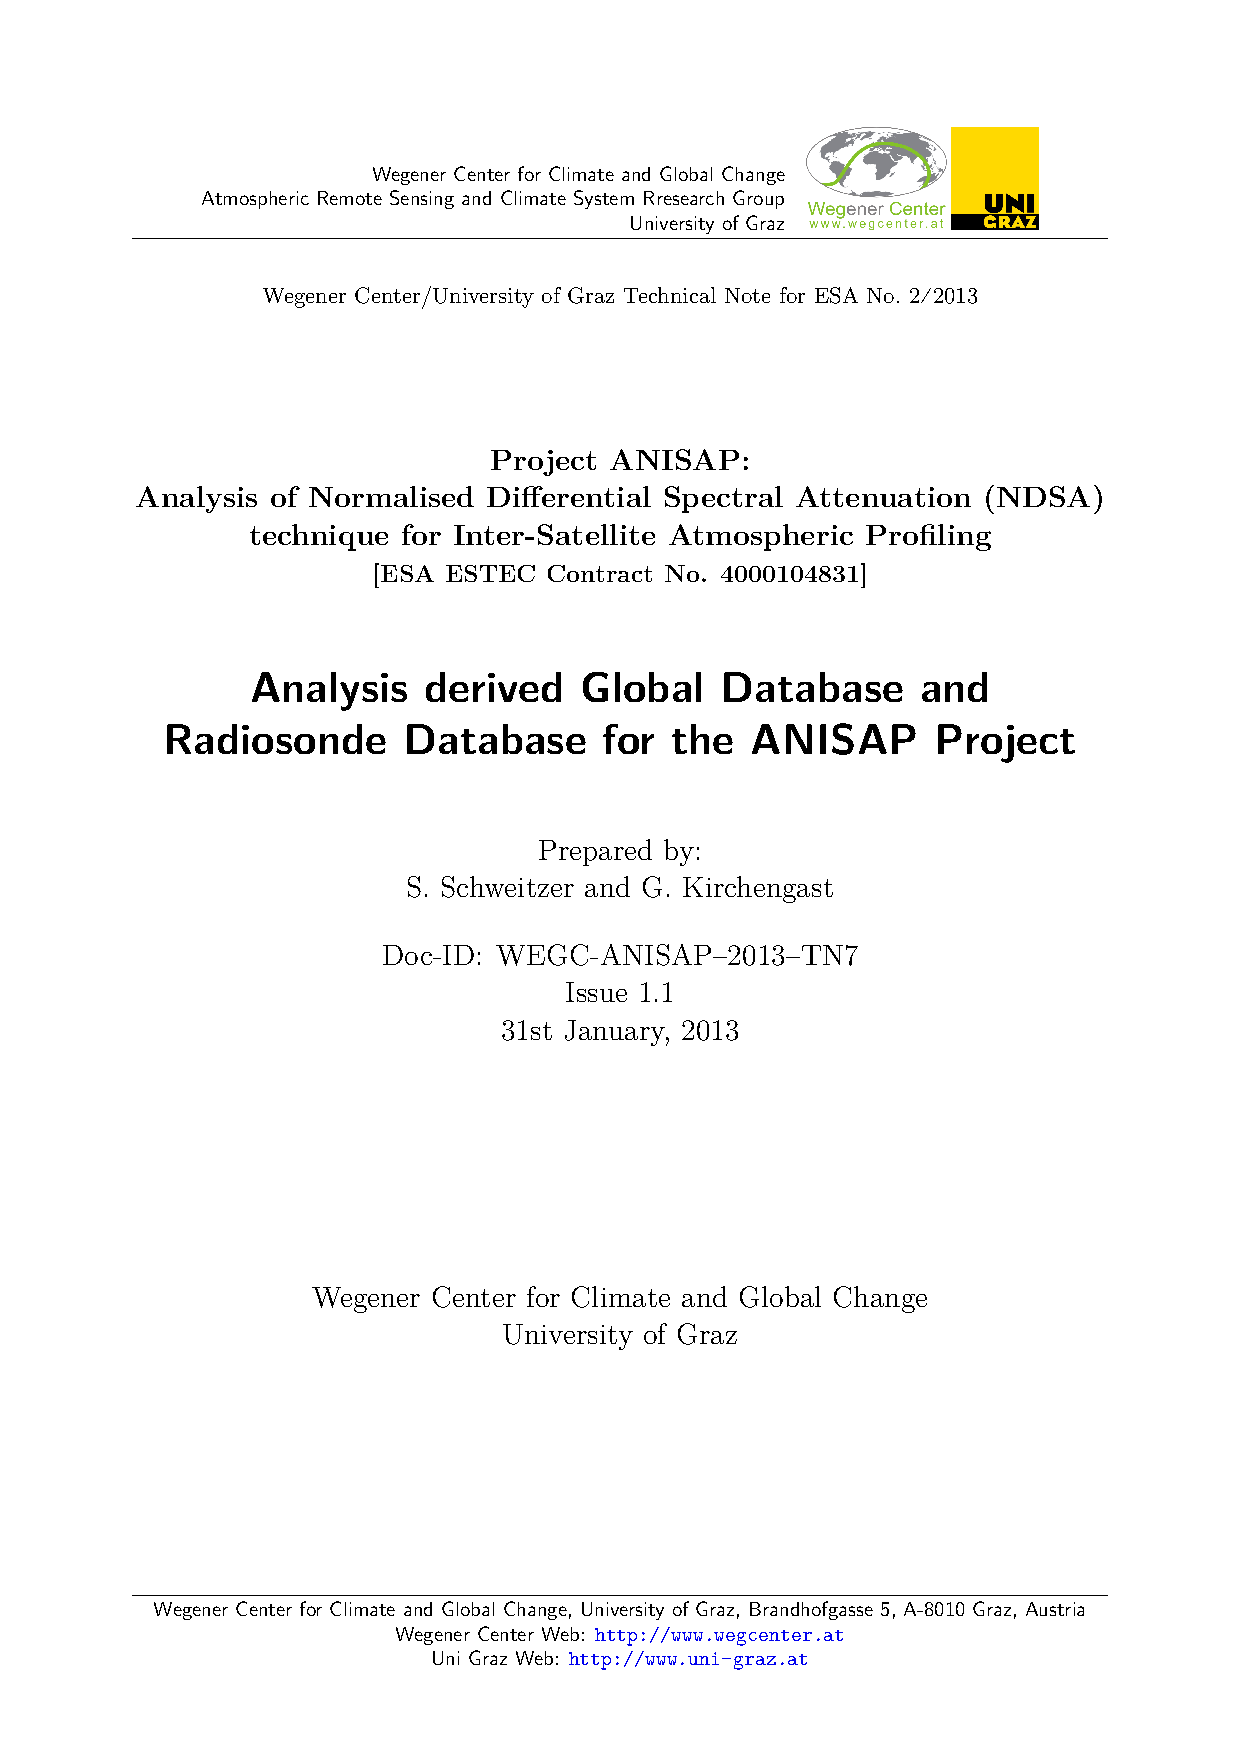
\includegraphics[height=0.7\paperheight, page=1]{anisap-TN2.pdf}}
  \caption{Example of a \multidoc document title page}
  \label{fig:multiDocTitlepage}
\end{figure}

\begin{figure}
  \centering
  \fbox{\includegraphics[height=0.7\paperheight, page=2]{anisap-TN2.pdf}}
  \caption{Example of a \multidoc document release information page}
  \label{fig:multiDocReleaseInfopage}
\end{figure}

\begin{figure}
  \centering
  \fbox{\includegraphics[height=0.7\paperheight, page=3]{anisap-TN2.pdf}}
  \caption{Example of a \multidoc document distribution list page}
  \label{fig:multiDocDistributionList}
\end{figure}

\begin{figure}
  \centering
  \fbox{\includegraphics[height=0.7\paperheight, page=4]{anisap-TN2.pdf}}
  \caption{Example of a \multidoc document change record page}
  \label{fig:multiDocChangeRecord}
\end{figure}

\begin{figure}
  \centering
  \fbox{\includegraphics[height=0.7\paperheight, page=10]{anisap-TN2.pdf}}
  \caption{Example of a \multidoc document random page}
  \label{fig:multiDocHeadings}
\end{figure}



\subsubsection[Document headings]{Tailoring the document headings}
\label{subsubsec:multiDocumentHeadings}

The layout of the document headings (\IE{} the header for the running
pages, see \autoref{fig:multiDocHeadings}) is the same for article, book
and report documents and is structured into three parts:
\begin{enumerate}
\item a four line text block on the left side (the exact definition of the
  concatenation of the string components is given in
  \autoref{lst:docstyleDocumentHeadingsTextBlock}) comprising
  \begin{enumerate}
  \item the document header title (built as a concatenated string from the
    document header title substring \latexcmd{\ThisDocHeaderTitleSubstr}
    and the document subtitle string \latexcmd{\ThisDocSubtitle}
  \item the document identifier (build as a concatenated string from the
    document identifier substring \latexcmd{\ThisDocIdSubstr}, the document
    release year \latexcmd{\ThisDocYear}, the document type%
    \footnote{The acronyms used for the various document types need to be
      defined in the file \path{acronyms.sty}, see
      \fullautoref{subsec:UsingTheAcronymDatabase}.}
    \latexcmd{\ThisDocType} (\EG{} \acs{tr} (\acl{tr}) or \acs{ar}
    (\acl{ar})), and the document internal number
    \latexcmd{\ThisDocIntNum})
  \item the document version (build as a concatenated string from the
    document issue number \latexcmd{\ThisDocIssue} and the document
    revision number \latexcmd{\ThisDocRevision}), and
  \item the document release date
  \end {enumerate}
\item a central single text line indicating the respective current section
  or chapter number and section or chapter title, and
\item a graphics block (of corporate logos) on the right side.
\end{enumerate}

The details and the structure of the document headings are defined in the
file \path{docstyle.sty} near line 315 to 354 (see
\autoref{lst:docstyleDocumentHeadings}).

Since individual details for a specific document from a \multidoc
documentation task are different from document to document due to the
different document content, document type, document identifiers, document
issue, document revision, document release date \ETC{}, these details are
only predefined in the file \path{docstyle.sty}, and intended to be
specifically tailored in each individual document's masterfile.

In essence, a block of redefining \LaTeX{} commands has to be added
(between the two already present commands \latexcmd{\makeatletter} and
\latexcmd{\makeatother}) to the master file, similar to the example given
in \autoref{lst:documentHeadingsExample}.
%
\begin{CommandLineListing}[style=DefaultFileListing, print=true, xleftmargin=0pt, gobble=2, %
  caption={Definition of document headings in the masterfile}, %
  label=lst:documentHeadingsExample]
  \makeatletter

  \renewcommand*{\ThisDocType}{%
    tr%
  }
  \renewcommand*{\ThisDocExtNum}{%
    03%
  }
  \renewcommand*{\ThisDocIntNum}{%
    37%
  }
  \renewcommand*{\ThisDocIssue}{%
    1%
  }
  \renewcommand*{\ThisDocRevision}{%
    3%
  }
  \renewcommand*{\subtitlePrefix}{%
    %
  }
  \renewcommand*{\ThisDocSubtitle}{%
    WLG Quickstart Guide%
  }
  \renewcommand*{\ThisDocHeaderTitleSubstr}{%
    \wegcLaTeX{}%
  }
  \renewcommand*{\ThisDocIdSubstr}{%
    \aces{wegc}-WLG-QSG%
  }
  \newdate{ThisDocDate}{13}{8}{2025}
  \renewcommand*{\ThisDocDate}{%
    \displaydate{ThisDocDate}%
  }
  \renewcommand*{\ThisDocYear}{%
    %% \getdateyear{ThisDocDate}%
    2028%
  }

  \makeatother
\end{CommandLineListing}

\lstinputlisting[style=DefaultFileListing, print=true,
   firstnumber=212, firstline=212, stepnumber=1, lastline=236,
   emptylines=*0,
   breaklines=true,
  caption={Definition of the documents headings text block in \texttt{\lstname}},
  label=lst:docstyleDocumentHeadingsTextBlock]{docstyle.sty}

\begin{landscape}
\lstinputlisting[style=DefaultFileListing, print=true,
   firstnumber=315, firstline=315, stepnumber=1, lastline=354,
   emptylines=*0,
   breaklines=true,
  caption={Definition of the document headings in \texttt{\lstname}},
  label=lst:docstyleDocumentHeadings]{docstyle.sty}
\end{landscape}


\subsubsection[Title page common elements]{Tailoring the common elements of the title page}
\label{subsubsec:multiDocumentTitlePageCommons}

The layout of the document title page is the same for article, book and
report documents and contains elements, which are common and the same for
all documents of a documentation task, \IE{} the title page header, the
title page footer, the document publisher details, the title head and the
subject details, and those that are different due to the individual
document content, \EG{} the document title or the document authors.


\minisec{Title page header and footer}

The common elements title page header and title page footer are defined and
specified in the file \path{docstyle.sty} near lines 252 and 271 (see
\autoref{lst:docstyleTitlepageHeaderFooter}).

\lstinputlisting[style=DefaultFileListing, print=true,
   firstnumber=252, firstline=252, stepnumber=1, lastline=281,
   emptylines=*1,
  caption={Definition of title page header and footer details in \texttt{\lstname}},
  label=lst:docstyleTitlepageHeaderFooter]{docstyle.sty}

If, for example, the combined \ac{igam}/\ac{wegc} title page header and
footer shall be replaced with the plain \ac{wegc} title page header and
footer, then the corresponding section in file \path{docstyle.sty} is to
be modified as shown in
\autoref{lst:docstyleTitlepageHeaderFooterWegcOnly}.
%
\begin{CommandLineListing}[style=DefaultFileListing, print=true, xleftmargin=0pt, gobble=2, %
  caption={Alternate definition of title page header and footer in \latexcmd{docstyle.sty}}, %
  label=lst:docstyleTitlepageHeaderFooterWegcOnly]
  \newcommand*{\Head@@ThisDocTitlePage}{%
    \upshape%
    \begin{varwidth}[b][0pt]{\paperwidth}%
      \LaTeXraggedleft%
      \Name{wegc}\\%
      %% \Name{igam}\\%
      \Name{ug}%
    \end{varwidth}%
    \quad%
    \begin{varwidth}[b][0pt]{\paperwidth}%
      
\includegraphics[height=50.0pt]{logo-ug-medium}%
      \hspace{2.0pt}%
      
\includegraphics[height=50.0pt]{logo-wegc-medium}%
      %% \hspace{2.0pt}%
      %% 
\includegraphics[height=50.0pt]{logo-igam-medium}%
    \end{varwidth}%
  }

  \newcommand*{\Foot@@ThisDocTitlePage}{%
    \upshape%
    \begin{varwidth}[t][0pt]{\paperwidth}%
      \LaTeXcentering%
      \Address{wegc}\\%
      %% \Address{igam}\\%
      \ShortName{wegc} Web\p: \WebAddress{wegc}\\%
      %% \ShortName{igam} Web\p: \WebAddress{igam}\\%
      \ShortName{ug} Web\p: \WebAddress{ug}\\%
    \end{varwidth}%
  }
\end{CommandLineListing}


\minisec{Title head and title subject details}

The title head and title subject details for the title page are defined in
the file \path{docstyle.sty} near lines 444 to 471 (see
\autoref{lst:docstyleTitlepageTitleheadSubject}).

\lstinputlisting[style=DefaultFileListing, print=true,
   firstnumber=444, firstline=444, stepnumber=1, lastline=471,
   emptylines=*0,
   caption={Definition of the title page title head and subject details in \texttt{\lstname}},
   label=lst:docstyleTitlepageTitleheadSubject]{docstyle.sty}

For changing the title page title head and subject details to something
different, the corresponding section in file \path{docstyle.sty} could
be modified as shown in
\autoref{lst:docstyleTitlepageTitleheadSubjectExample}.
%
\begin{CommandLineListing}[style=DefaultFileListing, print=true, xleftmargin=0pt, gobble=2, %
  caption={Alternate definition of title page title head and subject details in \latexcmd{docstyle.sty}}, %
  label=lst:docstyleTitlepageTitleheadSubjectExample]
  \newcommand*{\titleheadSubstr}{%
    \aces{wegc}%
  }
  \newcommand*{\titleheadSubSubstr}{%
    \aces{esa}%
  }
  \titlehead{%
    \makebox[\linewidth]{\titleheadSubstr \hbox{} \acel{\ThisDocType} for \titleheadSubSubstr \hbox{} \No{} \ThisDocExtNum\textfractionsolidus\ThisDocYear}%
  }
  \newcommand*{\subjectStr}{%
    rOPS Project\p:\\%
  }
  \newcommand*{\subjectSubstr}{%
    Typesetting and Document Generation%
  }
  \subject{%
    \subjectStr\subjectSubstr%
  }
\end{CommandLineListing}


\minisec{Publisher information}

The document publisher information for the title page is defined in the
file \path{docstyle.sty} near lines 504 to 520 (see
\autoref{lst:docstyleTitlepagePublisher}).

\lstinputlisting[style=DefaultFileListing, print=true,
   firstnumber=504, firstline=504, stepnumber=1, lastline=520,
   emptylines=*0,
   caption={Definition of the title page publisher details in \texttt{\lstname}},
   label=lst:docstyleTitlepagePublisher]{docstyle.sty}

For changing the title page publisher details to the plain \ac{wegc}
title page publisher details, the corresponding section in file
\path{docstyle.sty} is to be modified as shown in
\autoref{lst:docstyleTitlepagePublisherWegcOnly}.
%
\begin{CommandLineListing}[style=DefaultFileListing, print=true, xleftmargin=0pt, gobble=2, %
  caption={Alternate definition of title publisher details in \latexcmd{docstyle.sty}}, %
  label=lst:docstyleTitlepagePublisherWegcOnly]
  \newcommand*{\publishersSubstr}{%
    \acl{wegc}%
  }
  \newcommand*{\publishersSubSubstr}{%
    \acl{ug}%
  }
  \newcommand*{\publishersSubSubSubstr}{%
    %
  }
  \publishers{%
    \publishersSubstr\\\publishersSubSubstr\\\publishersSubSubSubstr%
  }
\end{CommandLineListing}


\minisec{Glossary and bibliography preambles}

If the default text for the preamble to the \emph{acronyms} and
\emph{abbreviations}, to the \emph{terms} and \emph{definitions}, or to the
bibliography does not fit as expected, these preambles can be modified in
\path{docstyle.sty}, starting near line 657 (see
\autoref{lst:docstyleGlossaryPreambles}) and near line 683 (see
\autoref{lst:docstyleBibliographyPreambles}).

\lstinputlisting[style=DefaultFileListing, print=true,
   firstnumber=657, firstline=657, stepnumber=1, lastline=670,
   emptylines=*0,
   caption={Definition of the glossary preambles in \texttt{\lstname}},
   label=lst:docstyleGlossaryPreambles]{docstyle.sty}

\lstinputlisting[style=DefaultFileListing, print=true,
   firstnumber=683, firstline=683, stepnumber=1, lastline=696,
   emptylines=*0,
   caption={Definition of the bibliography preambles in \texttt{\lstname}},
   label=lst:docstyleBibliographyPreambles]{docstyle.sty}


\subsubsection[Title page specific elements]{Tailoring the document specific elements of the title page}
\label{subsubsec:multiDocumentTitlePageSpecifics}

The layout of the document specific elements document title and authors are
predefined in the file \path{docstyle.sty} and need to be updated in each
individual document's masterfile by a block of redefining \LaTeX{} commands
which are to be added between the two already present commands
\latexcmd{\makeatletter} and \latexcmd{\makeatother}, similar to the
example given in \autoref{lst:documenTitlepageTitleExample}.

All other document specific elements required for the title page like
document type, document identifiers, document issue, document revision,
document release date \ETC{}, have already been described for the document
headings in \autoref{subsubsec:multiDocumentHeadings}

\Attention{%
  In \autoref{lst:documenTitlepageTitleExample}, the definition of the
  document subtitle is not explicitly shown, as it is already presented in
  \autoref{lst:documentHeadingsExample} of
  \autoref{subsubsec:multiDocumentHeadings} (due to the fact that
  \latexcmd{\subtitlePrefix} and \latexcmd{\ThisDocSubtitle} are used for
  the definition of the document headings).}

\begin{CommandLineListing}[style=DefaultFileListing, print=true, xleftmargin=0pt, gobble=2, %
  caption={Definition of document title and author details in the masterfile}, %
  label=lst:documenTitlepageTitleExample]
  \makeatletter
  ...
  ...
  \renewcommand*{\ThisDocTitle}{%
    The \wegcLaTeX{} documentation framework: \newline a guide for beginners%
  }
  \renewcommand*{\titlePrefix}{%
    %
  }
  \renewcommand*{\ThisDocAuthors}{%
    \ShortName{kmf}, \ShortName{jfb}, and \ShortName{gki}%
  }
  \makeatother
\end{CommandLineListing}


\subsubsection[A \multidoc document article]{Creating a \multidoc document article}
\label{subsubsec:creatingMultiDocumentArticle}

For creating a \multidoc article, proceed as follows:
%%
\begin{enumerate}
\item create a working directory for building the \wegcLaTeX{} \multidoc article, \\
  \EG{} \path{/home/\plh{user}/wlMultiDocTest/}

\item create the following subdirectories \\
  \path{/home/\plh{user}/wlMultiDocTest/wlg/}, \\
  \path{/home/\plh{user}/wlMultiDocTest/wlg/figs/}, \\
  \path{/home/\plh{user}/wlMultiDocTest/wlg/data/}, \\
  \path{/home/\plh{user}/wlMultiDocTest/wlg/tex/}, \\
  \path{/home/\plh{user}/wlMultiDocTest/common/}, and \\
  \path{/home/\plh{user}/wlMultiDocTest/common/figs}

  \Attention{Any further documents of a \multidoc documentation task would
    require the additional subdirectories \\
    \path{/home/\plh{user}/wlMultiDocTest/wlg2/}, \\
    \path{/home/\plh{user}/wlMultiDocTest/wlg2/figs/}, \\
    \path{/home/\plh{user}/wlMultiDocTest/wlg2/data/}, \\
    \path{/home/\plh{user}/wlMultiDocTest/wlg2/tex/}, \\
    and so on.}

\item copy the \LaTeX{} template master file \\
  \path{./texmf/doc/latex/wegc-latex/examples/multidoc-article/doc-article.tex} to \\
  \path{/home/\plh{user}/wlMultiDocTest/wlg/}

\item copy the seven \LaTeX{} source code files from \\
  \path{./texmf/doc/latex/wegc-latex/WLG/} to \\
  \path{/home/\plh{user}/wlMultiDocTest/wlg/tex/}

\item copy the twelve \path{*.png} and twelve \path{*.xbb} files from \\
  \path{./texmf/doc/latex/wegc-latex/examples/common/figs/} to \\
  \path{/home/\plh{user}/wlMultiDocTest/common/figs/}

\item copy the three files
  \path{docstyle.sty}, \path{project.sty}, and \path{commands.sty} from \\
  \path{./texmf/doc/latex/wegc-latex/examples/common/} to \\
  \path{/home/\plh{user}/wlMultiDocTest/common}

 \item extract the three example only files \path{acronyms.sty}, \path{addresses.sty}, and
  \path{terms.sty} from the compressed archive file \\
  \path{./texmf/doc/latex/wegc-latex/WLG/acronymsAddressesTerms_ExampleDoNotUse.tar.gz}
  or use the current and up to date versions available at 
  \nolinkurl{https://wegc203117.uni-graz.at/projects/latex_dbs/browser/arsclisys}
  and put them to \\
  \path{/home/\plh{user}/wlMultiDocTest/common}

\item add the address for the fictive person ``\Name{kmf}'' at the end of
  the copied file \path{addresses.sty}, as described in
  \autoref{subsec:usingTheAddressBookDatabase}

\item add the acronym for the fictive company ``\acf{tmc}'' at the end of
  the copied file \path{acronyms.sty}, as described in
  \autoref{subsec:UsingTheAcronymDatabase}

\item add the glossary entry for the fictive term ``\Gls{firlefanzation}''
  at the end of the copied file \path{terms.sty}, as described in
  \autoref{subsec:UsingTheGlossaryDatabase}

\item create an example bibliography file \path{exampleBibFile.bib} in the \\
  \path{/home/\plh{user}/wlMultiDocTest/wlg} directory in the same way as
  it is described for a \singledoc article (see
  \autoref{subsubsec:creatingSingleDocumentArticle})

\item copy the template master file \\
  \path{/home/\plh{user}/wlMultiDocTest/wlg/doc-wlarticle.tex} to \\
  \path{/home/\plh{user}/wlMultiDocTest/wlg/md-wlgArticle.tex} \\
  and apply the following modifications:
  \begin{enumerate}
  \item at line 119, change \latexcmd{DIV=default} to \latexcmd{DIV=11}
  \item between the lines 165 to 171, reading
    \begin{CommandLineListing}[style=DefaultFileListing, print=true, basicstyle={\ttfamily\small}, %
      basewidth=0.47em, xleftmargin=0pt, gobble=6]
      \makeatletter
      %% NOTE: Here, we can act as class and package authors if we want or need to do so ...
      \makeatother
    \end{CommandLineListing}
    add the definition commands for defining the document specific settings:
    \begin{CommandLineListing}[style=DefaultFileListing, print=true, basicstyle={\ttfamily\small}, %
      basewidth=0.47em, xleftmargin=0pt, gobble=6]
      \makeatletter

      \renewcommand*{\ThisDocType}{%
        tr%
      }
      \renewcommand*{\ThisDocExtNum}{%
        03%
      }
      \renewcommand*{\ThisDocIntNum}{%
        37%
      }
      \renewcommand*{\ThisDocIssue}{%
        1%
      }
      \renewcommand*{\ThisDocRevision}{%
        3%
      }
      \renewcommand*{\subtitlePrefix}{%
        %
      }
      \renewcommand*{\ThisDocSubtitle}{%
        WLG Quickstart Guide%
      }
      \renewcommand*{\ThisDocHeaderTitleSubstr}{%
        \wegcLaTeX{}%
      }
      \renewcommand*{\ThisDocIdSubstr}{%
        \aces{wegc}-WLG-QSG%
      }
      \newdate{ThisDocDate}{13}{8}{2025}
      \renewcommand*{\ThisDocDate}{%
        \displaydate{ThisDocDate}%
      }
      \renewcommand*{\ThisDocYear}{%
        %% \getdateyear{ThisDocDate}%
        2028%
      }
      \renewcommand*{\ThisDocTitle}{%
        The \wegcLaTeX{} documentation framework: \newline a guide for beginners%
      }
      \renewcommand*{\titlePrefix}{%
        %
      }
      \renewcommand*{\ThisDocAuthors}{%
        \ShortName{kmf}, \ShortName{jfb}, and \ShortName{gki}%
      }
      \makeatother
    \end{CommandLineListing}

  \item on lines 150 to 151: change from
    \begin{CommandLineListing}[style=DefaultFileListing, print=true, basicstyle={\ttfamily\small}, %
      basewidth=0.47em, xleftmargin=0pt, gobble=6]
      \bibliography{%
      }
    \end{CommandLineListing}
    to
    \begin{CommandLineListing}[style=DefaultFileListing, print=true, basicstyle={\ttfamily\small}, %
      basewidth=0.47em, xleftmargin=0pt, gobble=6]
      \bibliography{%
        exampleBibFile%
      }
    \end{CommandLineListing}

  \item between lines 165 and 171, reading
    \begin{CommandLineListing}[style=DefaultFileListing, print=true, basicstyle={\ttfamily\small}, %
      basewidth=0.47em, xleftmargin=0pt, gobble=6]
      \makeatletter

      %% NOTE: Here, we can act as class and package authors if we want or need to do so ...

      \makeatother
    \end{CommandLineListing}
    add the following command definitiosn for \entity{singledoc} and \entity{multidoc}:
    \begin{CommandLineListing}[style=DefaultFileListing, print=true, basicstyle={\ttfamily\small}, %
      basewidth=0.47em, xleftmargin=0pt, gobble=6]
      \makeatletter

      %% NOTE: Here, we can act as class and package authors if we want or need to do so ...

      \newcommand*{\singledoc}{%
        \entity{singledoc} %
      }

      \newcommand*{\multidoc}{%
        \entity{multidoc} %
      }

      \makeatother
    \end{CommandLineListing}

  \item \label{item:nociteGlsaddIncludeDirectives} between the lines 201
    and 204, reading
    \begin{CommandLineListing}[style=DefaultFileListing, print=true, basicstyle={\ttfamily\small}, %
      basewidth=0.47em, xleftmargin=0pt, gobble=6]
      \printbibliography[prenote=refpreamble]


      \appendix
    \end{CommandLineListing}
    add the following content:
    \begin{CommandLineListing}[style=DefaultFileListing, print=true, basicstyle={\ttfamily\small}, %
      basewidth=0.47em, xleftmargin=0pt, gobble=6]
      \printbibliography[prenote=refpreamble]

      \nocite{Gorbunov2007a}
      \nocite{Gorbunov2002a}
      \nocite{Gorbunov1986}

      \glsadd{development_team}
      \glsadd{firlefanzation}

      \glsadd{urd}
      \glsadd{add}
      \glsadd{ddd}
      \glsadd{sum}
      \glsadd{atr}

      \include{WLG-1_introduction}
      \include{WLG-2_installation}
      \include{WLG-3_documentGeneration}
      \include{WLG-4_commandsAndEnvironments}
      \include{WLG-5_practicalTips}
      \include{WLG-6_usingTheTemplates}
      \include{WLG-7_undocumentedTopics}

      \appendix
    \end{CommandLineListing}
   \end{enumerate}

 \item modify in the file
   \path{/home/\plh{user}/wlMultiDocTest/common/docstyle.sty} the titlepage
   header, titlepage footer, titlehead, subject and publisher details as
   described in \autoref{subsubsec:multiDocumentTitlePageCommons}.

 \item Finally, compile the master file
   \path{/home/\plh{user}/wlMultiDocTest/wlg/md-wlgArticle.tex} as
   described in \autoref{subsec:commandsForDocumentGeneration}.
\end{enumerate}


\subsubsection[A \multidoc document report]{Creating a \multidoc document report}
\label{subsubsec:creatingMultiDocumentReport}

For creating a \multidoc report, copy the \LaTeX{} template master file \\
\path{./texmf/doc/latex/wegc-latex/examples/multidoc-report/doc-report.tex} to \\
\path{/home/\plh{user}/wlMultiDocTest/wlg/}, \\
copy the file \\
\path{/home/\plh{user}/wlMultiDocTest/wlg/doc-wlreport.tex} to \\
\path{/home/\plh{user}/wlMultiDocTest/wlg/md-wlgReport.tex}, \\
and perform all other steps similar to the description in
\autoref{subsubsec:creatingMultiDocumentArticle}, considering the following
differences:
%%
\begin{enumerate}

\item in file \path{/home/\plh{user}/wlMultiDocTest/wlg/md-wlgReport.tex},
  \begin{enumerate}
  \item \label{item:nociteGlsaddIncludeMdReport} between the lines 213 and
    216 (\IE{} between the \latexcmd{\printbibliography} and
    \latexcmd{\appendix} commands), add the same \LaTeX{} commands
    \latexcmd{\nocite}, \latexcmd{\glsadd} and \latexcmd{\include} as
    indicated in \autoref{subsubsec:creatingMultiDocumentArticle},
    \autoref{item:nociteGlsaddIncludeDirectives}

  \item between the lines 213 and 216 (\IE{} between the
    \latexcmd{\printbibliography} and \latexcmd{\appendix} commands and
    immediately after the added statements of
    \autoref{item:nociteGlsaddIncludeMdReport}), add the definition of the
    \entity{Document Release Information} table, the \entity{Document
      Distribution List} and the \entity{Document Change Record}, as shown
    in \autoref{lst:exampleReleaseDistributionChangeRecord}
  \end{enumerate}

\item modify the document structuring directives \latexcmd{\section},
  \latexcmd{\subsection} and \latexcmd{\subsubsection} used in the seven
  \LaTeX{} files to \latexcmd{\chapter}, \latexcmd{\section} and
  \latexcmd{\subsection}, adapting it to the proper sectioning for report
  documents (similar to \autoref{subsubsec:creatingSingleDocumentReport}
  \autoref{item:modifyStructuringDirectives}).

\item Finally, compile the master file
  \path{/home/\plh{user}/wlMultiDocTest/wlg/md-wlgReport.tex} as described
  in \autoref{subsec:commandsForDocumentGeneration}.

\end{enumerate}


\begin{CommandLineListing}[style=DefaultFileListing, print=true, basicstyle={\ttfamily\small}, %
  basewidth=0.47em, xleftmargin=0pt, gobble=2, %
  caption={Definition of document release information, distribution list and change record}, %
  label=lst:exampleReleaseDistributionChangeRecord]
  \renewcommand*{\ThisAuthorizationIdentity}{%
    \ShortName{mip}, \ugorg{short}%
  }

  \renewcommand*{\ThisApprovalIdentity}{%
    \ShortName{gki}, \ugorg{short}%
  }

  %% \renewcommand*{\ThisDocReleaseInformationTab}{%
  %% \ifthenelse{\boolean{KOMAClass}}{\addsec*}{\section*}{Document Release Information}%
  %% \begin{tabularx}{\linewidth}[b]{@{}D@{}}%
  %%   \toprule%
  %%   \docid                                      & \ThisDocId                  \\%
  %%   Issue                                       & \ThisDocVersion             \\%
  %%   Date                                        & \ThisDocDate                \\%
  %%   Prepared by                                 & \ThisDocAuthors             \\%
  %%   Approved\textfractionsolidus{}Internally by & \ThisAuthorizationIdentity  \\%
  %%   Approved\textfractionsolidus{}Externally by & \ThisApprovalIdentity       \\%
  %%   \bottomrule%
  %% \end{tabularx}%
  %% }

  \renewcommand*{\ThisDocDistributionList}{%
    \ShortName{gki}       &  \aces{wegc}/\aces{ug}    & \EmailAddress{gki}       & 1\\%
    \small\ShortName{jfb} &  \aces{wegc}/\aces{ug}    & \small\EmailAddress{jfb} & 1\\%
    \Name{mip}            &  \aces{wegc}/\aces{ug}    & \EmailAddress{mip}       & 1%
  }

  \renewcommand*{\ThisDocChangeRecord}{%
    \software{short}{Version}{1}{0}{}{} &%
    \formatdate{20}{04}{2007} &%
    Original version of the document\p. \\ %
    %%
    \software{short}{Version}{1}{2}{}{} &%
    \formatdate{21}{12}{2008} &%
    Updates throughout the document by minor \newline
    changes and editorial corrections for clarification\p. \\ %
    %%
    \software{short}{Version}{\ThisDocIssue}{\ThisDocRevision}{}{}  &%
    \ThisDocDate &%
    Correction of minor inconsistencies\p.%
  }
\end{CommandLineListing}



\subsubsection[A \multidoc document book]{Creating a \multidoc document book}
\label{subsubsec:creatingMultiDocumentBook}

For creating a \multidoc book, copy the \LaTeX{} template master file \\
\path{./texmf/doc/latex/wegc-latex/examples/multidoc-book/doc-wlbook.tex} to \\
\path{/home/\plh{user}/wlMultiDocTest/wlg/}, copy the file \\
\path{/home/\plh{user}/wlMultiDocTest/wlg/doc-wlbook.tex} to \\
\path{/home/\plh{user}/wlMultiDocTest/wlg/md-wlgBook.tex} 
and perform all other steps similar to the description in
\autoref{subsubsec:creatingMultiDocumentArticle}, considering the following
differences:
%%
\begin{enumerate}

\item in file \path{/home/\plh{user}/wlMultiDocTest/wlg/md-wlgBook.tex},
  \begin{enumerate}
  \item \label{item:nociteGlsaddIncludeMdBook} between the lines 219 and
    222 (\IE{} between the \latexcmd{\mainmatter} and \latexcmd{\appendix}
    commands), add the same \LaTeX{} commands \latexcmd{\nocite},
    \latexcmd{\glsadd} and \latexcmd{\include} as indicated in
    \autoref{subsubsec:creatingMultiDocumentArticle},
    \autoref{item:nociteGlsaddIncludeDirectives}

  \item between the lines 219 and 222 (\IE{} between the
    \latexcmd{\mainmatter} and \latexcmd{\appendix} commands and
    immediately after the added statements of
    \autoref{item:nociteGlsaddIncludeMdBook}), add the definition of the
    \entity{Document Release Information} table, the \entity{Document
      Distribution List} and the \entity{Document Change Record}, as shown
    in \autoref{lst:exampleReleaseDistributionChangeRecord}
  \end{enumerate}

\item modify the document structuring directives \latexcmd{\section},
  \latexcmd{\subsection} and \latexcmd{\subsubsection} used in the seven
  \LaTeX{} files to \latexcmd{\chapter}, \latexcmd{\section} and
  \latexcmd{\subsection}, adapting it to the proper sectioning for book
  documents (similar to \autoref{subsubsec:creatingSingleDocumentReport}
  \autoref{item:modifyStructuringDirectives}).

\item Finally, compile the master file \\
  \path{/home/\plh{user}/wlMultiDocTest/wlg/md-wlgBook.tex} \\
  as described in \autoref{subsec:commandsForDocumentGeneration}.

\end{enumerate}

      


\section[Undocumented topics]{Undocumented topics}

Additionally, the following features are provided as an extension to the \KOMAScript{} bundle:
%
\begin{itemize}
   \item \latexcmd{\rowstyle} and column types \entity{=}, \entity{+}
   \item column type \entity{D}
   \item \latexcmd{\noacronymfont} (\entity{glossaries} package)
   \item \latexcmd{\acrentryshort} (\entity{glossaries} package) and similar commands + shortcuts
\end{itemize}

\noindent{}TODO Describe all packages loaded in \wegcLaTeX{}: What are they
for, basic functionality, basic commands.



      \appendix
    \end{CommandLineListing}

  \item near the lines 135, directly after the \latexcmd{\documentclass}
    directive, add the following commands:
    \begin{CommandLineListing}[style=DefaultFileListing, print=true, basicstyle={\ttfamily\small}, %
      basewidth=0.47em, xleftmargin=0pt, gobble=6]
      \RequirePackage{acronyms}
      \RequirePackage{terms}
      \RequirePackage{addresses}
      \RequirePackage{commands}
    \end{CommandLineListing}

  \end{enumerate}

\item Finally, compile the master file \\
  \path{/home/\plh{user}/wlSingleDocTest/wlg/wlgArticle.tex} \\
  as described in \autoref{subsec:commandsForDocumentGeneration}.
\end{enumerate}


\subsubsection[A \singledoc document report]{Creating a \singledoc document report}
\label{subsubsec:creatingSingleDocumentReport}

For creating a \singledoc report, copy the \LaTeX{} template master file \\
\path{./texmf/doc/latex/wegc-latex/examples/singledoc/master-wlreport.tex} to \\
\path{/home/\plh{user}/wlSingleDocTest/wlg/}. \\
Then copy the file \\
\path{/home/\plh{user}/wlSingleDocTest/wlg/master-wlreport.tex} to \\
\path{/home/\plh{user}/wlSingleDocTest/wlg/wlgReport.tex} \\
and perform all other steps similar to the description in
\autoref{subsubsec:creatingSingleDocumentArticle}, considering the
following differences:
%%
\begin{enumerate}
\item change the setting for \latexcmd{\extratitle},
  \latexcmd{\uppertitleback}, and \latexcmd{\lowertitleback} from
  \begin{CommandLineListing}[style=DefaultFileListing, print=true, basicstyle={\ttfamily\small}, %
    basewidth=0.47em, xleftmargin=0pt, gobble=4]
    \extratitle{%
      \highlight{\placeholder{My Bastard Title}}%
    }
    \uppertitleback{%
      \highlight{\placeholder{My Upper Title Back}}%
    }
    \lowertitleback{%
      \highlight{\placeholder{My Lower Title Back}}%
    }
  \end{CommandLineListing}
  to
  \begin{CommandLineListing}[style=DefaultFileListing, print=true, basicstyle={\ttfamily\small}, %
    basewidth=0.47em, xleftmargin=0pt, gobble=4]
    \extratitle{%
      %
    }
    \uppertitleback{%
      %
    }
    \lowertitleback{%
      %
    }
  \end{CommandLineListing}
  or to specific texts fitting the intended publication.

\item
  instead of
  \begin{CommandLineListing}[style=DefaultFileListing, print=true, basicstyle={\ttfamily\small}, %
    basewidth=0.47em, xleftmargin=0pt, gobble=4]
    \defbibnote{refpreamble}{%
      \highlight{\placeholder{My References Preamble}}%
    }
  \end{CommandLineListing}
  change it to
  \begin{CommandLineListing}[style=DefaultFileListing, print=true, basicstyle={\ttfamily\small}, %
    basewidth=0.47em, xleftmargin=0pt, gobble=4]
    \defbibnote{bibpreamble}{%
      %
    }
  \end{CommandLineListing}
  or to a specific text appropriate for the intended publication.

\item \label{item:modifyStructuringDirectives}
  modify the document structuring directives \latexcmd{\section},
  \latexcmd{\subsection} and \latexcmd{\subsubsection}
  used within the files \\
  \path{WLG-1_introduction}, \\
  \path{WLG-2_installation}, \\
  \path{WLG-3_documentGeneration}, \\
  \path{WLG-4_commandsAndEnvironments}, \\
  \path{WLG-5_practicalTips}, \\
  \path{WLG-6_usingTheTemplates}, and \\
  \path{WLG-7_undocumentedTopics} to \\
  \latexcmd{\chapter}, \latexcmd{\section} and \latexcmd{\subsection},
  adapting it to the proper sectioning for report documents.

\item place the \latexcmd{\include} directives for including the seven
  \LaTeX{} subdocument files between the \latexcmd{\printglossary} and
  \latexcmd{\appendix} commands.

\item Finally, compile the master file \path{wlgReport.tex} as described in
  \autoref{subsec:commandsForDocumentGeneration}.
\end{enumerate}



\subsubsection[A \singledoc document book]{Creating a \singledoc document book}
\label{subsubsec:creatingSingleDocumentBook}

For creating a \singledoc book, copy the \LaTeX{} template master file \\
\path{./texmf/doc/latex/wegc-latex/examples/singledoc/master-wlbook.tex} to \\
\path{/home/\plh{user}/wlSingleDocTest/wlg/}. \\
Then copy the file \\
\path{/home/\plh{user}/wlSingleDocTest/wlg/master-wlbook.tex} to \\
\path{/home/\plh{user}/wlSingleDocTest/wlg/wlgBook.tex} \\
and perform all other steps similar to the description in
\autoref{subsubsec:creatingSingleDocumentArticle}, considering the following differences:
%%
\begin{enumerate}
\item change the settings for \latexcmd{\extratitle},
  \latexcmd{\uppertitleback}, \latexcmd{\lowertitleback},\\
  \latexcmd{\upperinfopage}, \latexcmd{\lowerinfopage}, and
  \latexcmd{\lastpage} from
  \begin{CommandLineListing}[style=DefaultFileListing, print=true, basicstyle={\ttfamily\small}, %
    basewidth=0.47em, xleftmargin=0pt, gobble=4]
    \extratitle{%
      \highlight{\placeholder{My Bastard Title}}%
    }
    \uppertitleback{%
      \highlight{\placeholder{My Upper Title Back}}%
    }
    \lowertitleback{%
      \highlight{\placeholder{My Lower Title Back}}%
    }
    \upperinfopage{%
      \highlight{\placeholder{My Upper Info Page}}%
    }
    \lowerinfopage{%
      \highlight{\placeholder{My Lower Info Page}}%
    }
    \lastpage{%
      \highlight{\placeholder{My Last Page}}%
    }
  \end{CommandLineListing}
  to
  \begin{CommandLineListing}[style=DefaultFileListing, print=true, basicstyle={\ttfamily\small}, %
    basewidth=0.47em, xleftmargin=0pt, gobble=4]
    \extratitle{%
      %
    }
    \uppertitleback{%
      %
    }
    \lowertitleback{%
      %
    }
    \upperinfopage{%
      %
    }
    \lowerinfopage{%
      %
    }
    \lastpage{%
      %
    }
  \end{CommandLineListing}
  or to the specific texts fitting the intended publication.

\item instead of
  \begin{CommandLineListing}[style=DefaultFileListing, print=true,
    basicstyle={\ttfamily\small}, %
    basewidth=0.47em, xleftmargin=0pt, gobble=4]
    \defbibnote{refpreamble}{%
      \highlight{\placeholder{My References Preamble}}%
    }
  \end{CommandLineListing}
  change it to
  \begin{CommandLineListing}[style=DefaultFileListing, print=true,
    basicstyle={\ttfamily\small}, %
    basewidth=0.47em, xleftmargin=0pt, gobble=4]
    \defbibnote{bibpreamble}{%
      %
    }
  \end{CommandLineListing}
  or to a specific text appropriate for the intended publication.

\item modify the document structuring directives \latexcmd{\section},
  \latexcmd{\subsection} and \latexcmd{\subsubsection} used in the seven
  \LaTeX{} files to \latexcmd{\chapter}, \latexcmd{\section} and
  \latexcmd{\subsection}, adapting it to the proper sectioning for book
  documents (similar to \autoref{subsubsec:creatingSingleDocumentReport}
  \autoref{item:modifyStructuringDirectives}).

\item place the \latexcmd{\include} directives for including the seven
  \LaTeX{} subdocument files between the \latexcmd{\mainmatter} and
  \latexcmd{\appendix} commands.

\item finally, compile the master file \path{wlgBook.tex} as described in
  \autoref{subsec:commandsForDocumentGeneration}.

\end{enumerate}



\subsubsection[A \singledoc \ac{msc} or \ac{phd} thesis]{Creating a \singledoc \ac{msc} or \ac{phd} thesis}
\label{subsubsec:creatingMasterOrPhdThesis}

For creating a \singledoc \ac{msc} or \ac{phd} thesis, generally proceed as 
described in the previous \fullautoref{subsubsec:creatingSingleDocumentBook}, 
dealing with a generic \singledoc document book, but change the document title page
similar to the example provided in \autoref{lst:coverPageMasterOrPhdThesis}.  

\begin{CommandLineListing}[style=DefaultFileListing, print=true, basicstyle={\ttfamily\small}, %
                           basewidth=0.47em, xleftmargin=0pt, gobble=3, %
                           caption={Example of a \ac{msc} or \ac{phd} thesis cover page}, %
                           label=lst:coverPageMasterOrPhdThesis]
   %%-------------------------------------------------------------------------%%
   \SetUpPrimaryPageStyle{scrheadings}
   %%
   \renewcommand*{\titlepagestyle}{%
     empty%
   }
   \renewcommand*{\extratitlepagestyle}{%
     empty%
   }
   %%-------------------------------------------------------------------------%%
   %% \extratitle{%
   %%   \highlight{\placeholder{My Bastard Title}}%
   %% }
   %%-------------------------------------------------------------------------%%
   %% \titlehead{%
   %%   \highlight{\placeholder{My Title Head}}%
   %% }
   \subject{%
      \LARGE{Master Thesis} \vspace{2.5mm} \\
      \Large{to obtain the degree Master of Science} \vspace{2.5mm} \\
      \Large{at the Faculty of Natural Sciences} \\
      \Large{University of Graz}%
   }
   %%
   \title{%
     \Huge{Global temperature budget: \\
           Constraints from aircraft and \\
           radio occultation observations}%%
   }
   %%
   \subtitle{%
     %
   }
   %%
   \author{%
     \Large{Franz G. M\"uller, Bakk.rer.nat.}%
   }
   %%
   \date{%
     \large{March 2017}%
     \vspace{5mm}%
   }
   %%
   \publishers{%
      \large{%
      Supervisor: Univ.-Prof.\! Mag.\! Dr.rer.nat.\! Erika L. Mauerheimer%
      \vspace{1.5mm} \\
      Co{\hyphen}Supervisor: Mag.\! Dr.rer.nat.\! Detlef R\"ottbauer}%
      \vspace{7.0mm} \\
      \normalsize{%
      Wegener Center for Climate and Global Change (WEGC) and \\
      Institute for Geophysics, Astrophysics, and
      Meteorology \textfractionsolidus{} Institute of Physics \\
      University of Graz}%
      \vspace{5mm} \\
      
\includegraphics[width=5.5cm]{logo_unigraz_wegc_medium.png}
   }
   %%-------------------------------------------------------------------------%%
   \uppertitleback{%
     %% \highlight{\placeholder{My Upper Title Back}}%
   }
   %%
   \lowertitleback{%
     %% \highlight{\placeholder{My Lower Title Back}}%
   }
   %%-------------------------------------------------------------------------%%
   \upperinfopage{%
     \highlight{\placeholder{My Upper Info Page}}%
   }
   %%
   \lowerinfopage{%
     \highlight{\placeholder{My Lower Info Page}}%
   }
   %%-------------------------------------------------------------------------%%
   \lastpage{%
     \highlight{\placeholder{My Last Page}}%
   }
   %%-------------------------------------------------------------------------%%
   ...
   %% \makeinfopage
   ...
   %%-------------------------------------------------------------------------%%
\end{CommandLineListing}



\subsection[The \multidoc document templates]{Using \multidoc document templates}
\label{subsec:usingMultiDocumentTemplates}

The \multidoc templates are intended for publications that comprise two or
more articles, reports or books and which shall have a common and
consistent layout of the document front matter, \EG{} title page,
distribution list, document revision history, bibliography, lists of
figures and tables as well as document headings.

Sample pages for a \multidoc title page, document release information page,
document distribution list and document change record are provided in
\autoref{fig:multiDocTitlepage}, \autoref{fig:multiDocReleaseInfopage},
\autoref{fig:multiDocDistributionList} and
\autoref{fig:multiDocChangeRecord}.

\begin{figure}
  \centering
  \fbox{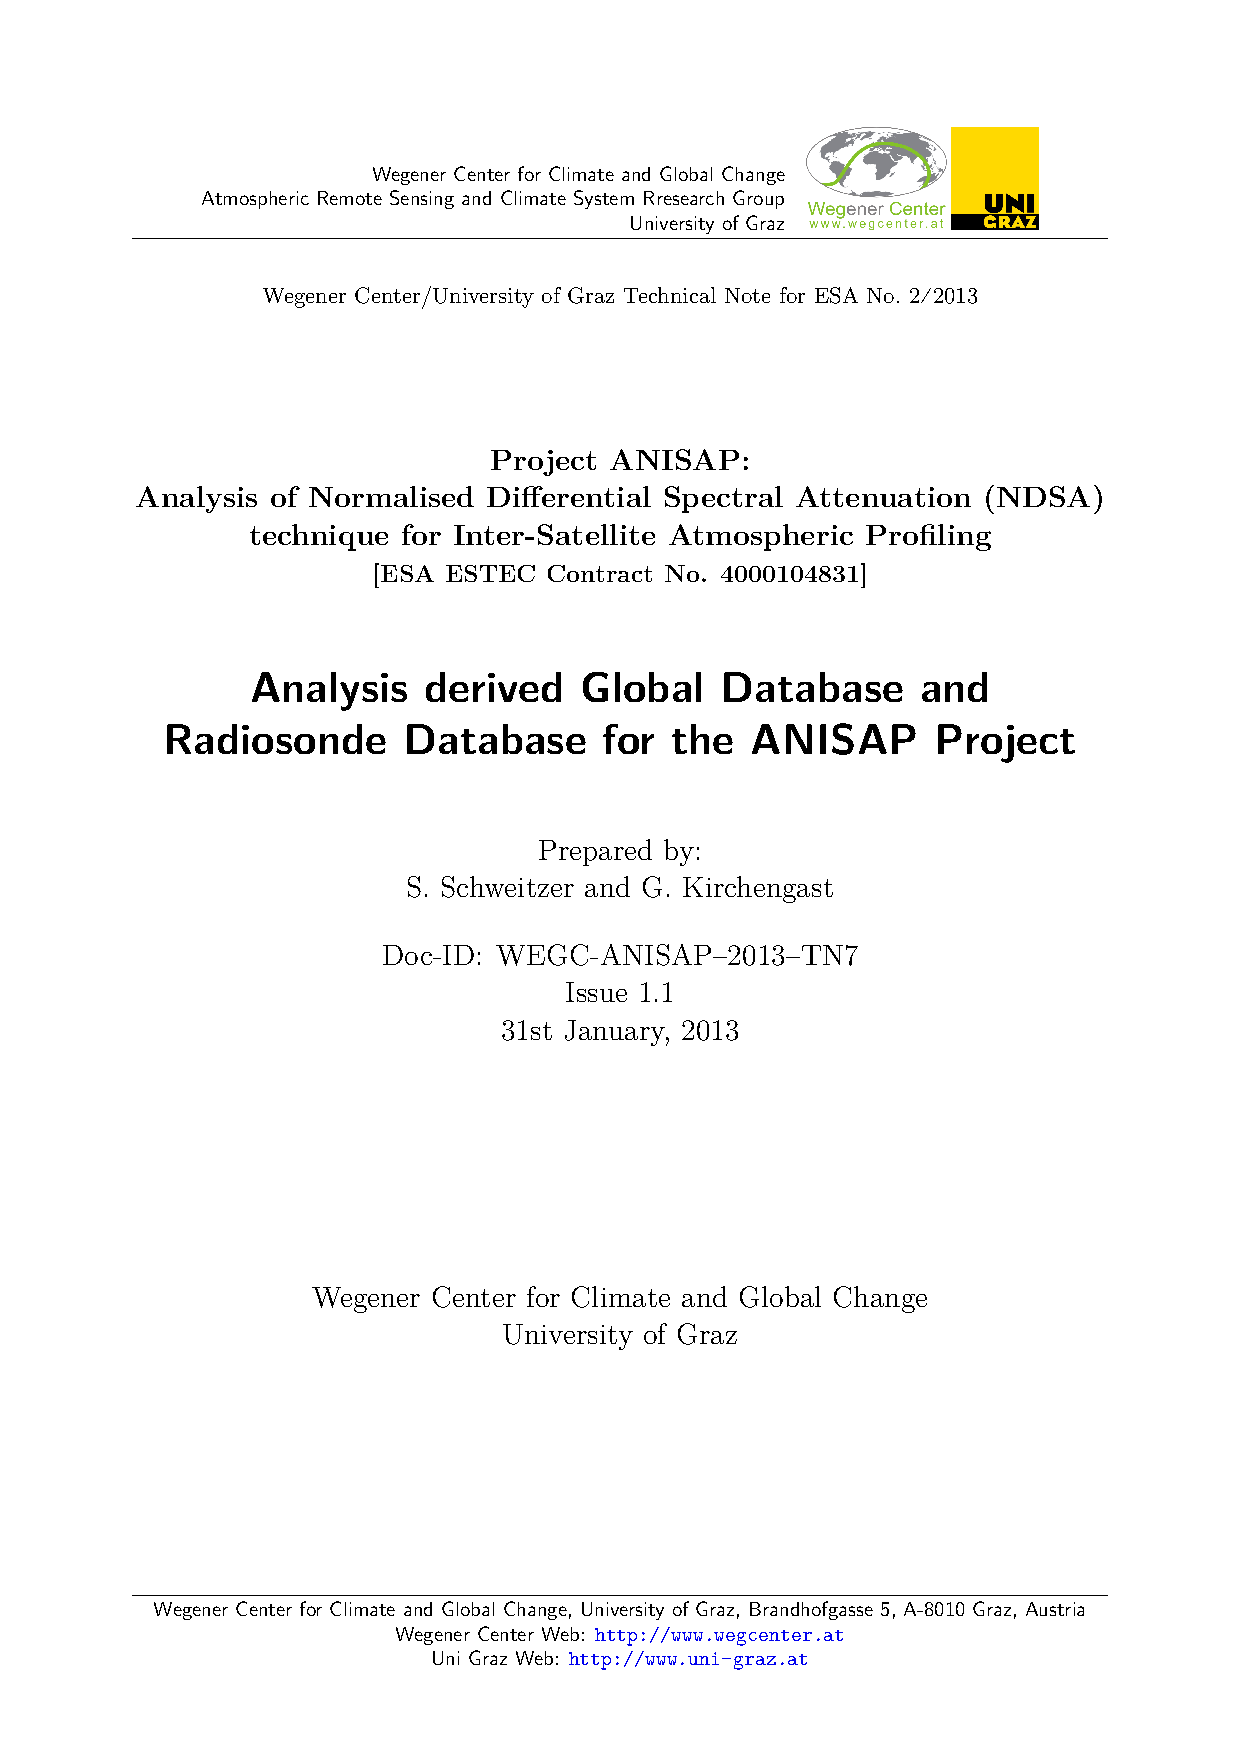
\includegraphics[height=0.7\paperheight, page=1]{anisap-TN2.pdf}}
  \caption{Example of a \multidoc document title page}
  \label{fig:multiDocTitlepage}
\end{figure}

\begin{figure}
  \centering
  \fbox{\includegraphics[height=0.7\paperheight, page=2]{anisap-TN2.pdf}}
  \caption{Example of a \multidoc document release information page}
  \label{fig:multiDocReleaseInfopage}
\end{figure}

\begin{figure}
  \centering
  \fbox{\includegraphics[height=0.7\paperheight, page=3]{anisap-TN2.pdf}}
  \caption{Example of a \multidoc document distribution list page}
  \label{fig:multiDocDistributionList}
\end{figure}

\begin{figure}
  \centering
  \fbox{\includegraphics[height=0.7\paperheight, page=4]{anisap-TN2.pdf}}
  \caption{Example of a \multidoc document change record page}
  \label{fig:multiDocChangeRecord}
\end{figure}

\begin{figure}
  \centering
  \fbox{\includegraphics[height=0.7\paperheight, page=10]{anisap-TN2.pdf}}
  \caption{Example of a \multidoc document random page}
  \label{fig:multiDocHeadings}
\end{figure}



\subsubsection[Document headings]{Tailoring the document headings}
\label{subsubsec:multiDocumentHeadings}

The layout of the document headings (\IE{} the header for the running
pages, see \autoref{fig:multiDocHeadings}) is the same for article, book
and report documents and is structured into three parts:
\begin{enumerate}
\item a four line text block on the left side (the exact definition of the
  concatenation of the string components is given in
  \autoref{lst:docstyleDocumentHeadingsTextBlock}) comprising
  \begin{enumerate}
  \item the document header title (built as a concatenated string from the
    document header title substring \latexcmd{\ThisDocHeaderTitleSubstr}
    and the document subtitle string \latexcmd{\ThisDocSubtitle}
  \item the document identifier (build as a concatenated string from the
    document identifier substring \latexcmd{\ThisDocIdSubstr}, the document
    release year \latexcmd{\ThisDocYear}, the document type%
    \footnote{The acronyms used for the various document types need to be
      defined in the file \path{acronyms.sty}, see
      \fullautoref{subsec:UsingTheAcronymDatabase}.}
    \latexcmd{\ThisDocType} (\EG{} \acs{tr} (\acl{tr}) or \acs{ar}
    (\acl{ar})), and the document internal number
    \latexcmd{\ThisDocIntNum})
  \item the document version (build as a concatenated string from the
    document issue number \latexcmd{\ThisDocIssue} and the document
    revision number \latexcmd{\ThisDocRevision}), and
  \item the document release date
  \end {enumerate}
\item a central single text line indicating the respective current section
  or chapter number and section or chapter title, and
\item a graphics block (of corporate logos) on the right side.
\end{enumerate}

The details and the structure of the document headings are defined in the
file \path{docstyle.sty} near line 315 to 354 (see
\autoref{lst:docstyleDocumentHeadings}).

Since individual details for a specific document from a \multidoc
documentation task are different from document to document due to the
different document content, document type, document identifiers, document
issue, document revision, document release date \ETC{}, these details are
only predefined in the file \path{docstyle.sty}, and intended to be
specifically tailored in each individual document's masterfile.

In essence, a block of redefining \LaTeX{} commands has to be added
(between the two already present commands \latexcmd{\makeatletter} and
\latexcmd{\makeatother}) to the master file, similar to the example given
in \autoref{lst:documentHeadingsExample}.
%
\begin{CommandLineListing}[style=DefaultFileListing, print=true, xleftmargin=0pt, gobble=2, %
  caption={Definition of document headings in the masterfile}, %
  label=lst:documentHeadingsExample]
  \makeatletter

  \renewcommand*{\ThisDocType}{%
    tr%
  }
  \renewcommand*{\ThisDocExtNum}{%
    03%
  }
  \renewcommand*{\ThisDocIntNum}{%
    37%
  }
  \renewcommand*{\ThisDocIssue}{%
    1%
  }
  \renewcommand*{\ThisDocRevision}{%
    3%
  }
  \renewcommand*{\subtitlePrefix}{%
    %
  }
  \renewcommand*{\ThisDocSubtitle}{%
    WLG Quickstart Guide%
  }
  \renewcommand*{\ThisDocHeaderTitleSubstr}{%
    \wegcLaTeX{}%
  }
  \renewcommand*{\ThisDocIdSubstr}{%
    \aces{wegc}-WLG-QSG%
  }
  \newdate{ThisDocDate}{13}{8}{2025}
  \renewcommand*{\ThisDocDate}{%
    \displaydate{ThisDocDate}%
  }
  \renewcommand*{\ThisDocYear}{%
    %% \getdateyear{ThisDocDate}%
    2028%
  }

  \makeatother
\end{CommandLineListing}

\lstinputlisting[style=DefaultFileListing, print=true,
   firstnumber=212, firstline=212, stepnumber=1, lastline=236,
   emptylines=*0,
   breaklines=true,
  caption={Definition of the documents headings text block in \texttt{\lstname}},
  label=lst:docstyleDocumentHeadingsTextBlock]{docstyle.sty}

\begin{landscape}
\lstinputlisting[style=DefaultFileListing, print=true,
   firstnumber=315, firstline=315, stepnumber=1, lastline=354,
   emptylines=*0,
   breaklines=true,
  caption={Definition of the document headings in \texttt{\lstname}},
  label=lst:docstyleDocumentHeadings]{docstyle.sty}
\end{landscape}


\subsubsection[Title page common elements]{Tailoring the common elements of the title page}
\label{subsubsec:multiDocumentTitlePageCommons}

The layout of the document title page is the same for article, book and
report documents and contains elements, which are common and the same for
all documents of a documentation task, \IE{} the title page header, the
title page footer, the document publisher details, the title head and the
subject details, and those that are different due to the individual
document content, \EG{} the document title or the document authors.


\minisec{Title page header and footer}

The common elements title page header and title page footer are defined and
specified in the file \path{docstyle.sty} near lines 252 and 271 (see
\autoref{lst:docstyleTitlepageHeaderFooter}).

\lstinputlisting[style=DefaultFileListing, print=true,
   firstnumber=252, firstline=252, stepnumber=1, lastline=281,
   emptylines=*1,
  caption={Definition of title page header and footer details in \texttt{\lstname}},
  label=lst:docstyleTitlepageHeaderFooter]{docstyle.sty}

If, for example, the combined \ac{igam}/\ac{wegc} title page header and
footer shall be replaced with the plain \ac{wegc} title page header and
footer, then the corresponding section in file \path{docstyle.sty} is to
be modified as shown in
\autoref{lst:docstyleTitlepageHeaderFooterWegcOnly}.
%
\begin{CommandLineListing}[style=DefaultFileListing, print=true, xleftmargin=0pt, gobble=2, %
  caption={Alternate definition of title page header and footer in \latexcmd{docstyle.sty}}, %
  label=lst:docstyleTitlepageHeaderFooterWegcOnly]
  \newcommand*{\Head@@ThisDocTitlePage}{%
    \upshape%
    \begin{varwidth}[b][0pt]{\paperwidth}%
      \LaTeXraggedleft%
      \Name{wegc}\\%
      %% \Name{igam}\\%
      \Name{ug}%
    \end{varwidth}%
    \quad%
    \begin{varwidth}[b][0pt]{\paperwidth}%
      
\includegraphics[height=50.0pt]{logo-ug-medium}%
      \hspace{2.0pt}%
      
\includegraphics[height=50.0pt]{logo-wegc-medium}%
      %% \hspace{2.0pt}%
      %% 
\includegraphics[height=50.0pt]{logo-igam-medium}%
    \end{varwidth}%
  }

  \newcommand*{\Foot@@ThisDocTitlePage}{%
    \upshape%
    \begin{varwidth}[t][0pt]{\paperwidth}%
      \LaTeXcentering%
      \Address{wegc}\\%
      %% \Address{igam}\\%
      \ShortName{wegc} Web\p: \WebAddress{wegc}\\%
      %% \ShortName{igam} Web\p: \WebAddress{igam}\\%
      \ShortName{ug} Web\p: \WebAddress{ug}\\%
    \end{varwidth}%
  }
\end{CommandLineListing}


\minisec{Title head and title subject details}

The title head and title subject details for the title page are defined in
the file \path{docstyle.sty} near lines 444 to 471 (see
\autoref{lst:docstyleTitlepageTitleheadSubject}).

\lstinputlisting[style=DefaultFileListing, print=true,
   firstnumber=444, firstline=444, stepnumber=1, lastline=471,
   emptylines=*0,
   caption={Definition of the title page title head and subject details in \texttt{\lstname}},
   label=lst:docstyleTitlepageTitleheadSubject]{docstyle.sty}

For changing the title page title head and subject details to something
different, the corresponding section in file \path{docstyle.sty} could
be modified as shown in
\autoref{lst:docstyleTitlepageTitleheadSubjectExample}.
%
\begin{CommandLineListing}[style=DefaultFileListing, print=true, xleftmargin=0pt, gobble=2, %
  caption={Alternate definition of title page title head and subject details in \latexcmd{docstyle.sty}}, %
  label=lst:docstyleTitlepageTitleheadSubjectExample]
  \newcommand*{\titleheadSubstr}{%
    \aces{wegc}%
  }
  \newcommand*{\titleheadSubSubstr}{%
    \aces{esa}%
  }
  \titlehead{%
    \makebox[\linewidth]{\titleheadSubstr \hbox{} \acel{\ThisDocType} for \titleheadSubSubstr \hbox{} \No{} \ThisDocExtNum\textfractionsolidus\ThisDocYear}%
  }
  \newcommand*{\subjectStr}{%
    rOPS Project\p:\\%
  }
  \newcommand*{\subjectSubstr}{%
    Typesetting and Document Generation%
  }
  \subject{%
    \subjectStr\subjectSubstr%
  }
\end{CommandLineListing}


\minisec{Publisher information}

The document publisher information for the title page is defined in the
file \path{docstyle.sty} near lines 504 to 520 (see
\autoref{lst:docstyleTitlepagePublisher}).

\lstinputlisting[style=DefaultFileListing, print=true,
   firstnumber=504, firstline=504, stepnumber=1, lastline=520,
   emptylines=*0,
   caption={Definition of the title page publisher details in \texttt{\lstname}},
   label=lst:docstyleTitlepagePublisher]{docstyle.sty}

For changing the title page publisher details to the plain \ac{wegc}
title page publisher details, the corresponding section in file
\path{docstyle.sty} is to be modified as shown in
\autoref{lst:docstyleTitlepagePublisherWegcOnly}.
%
\begin{CommandLineListing}[style=DefaultFileListing, print=true, xleftmargin=0pt, gobble=2, %
  caption={Alternate definition of title publisher details in \latexcmd{docstyle.sty}}, %
  label=lst:docstyleTitlepagePublisherWegcOnly]
  \newcommand*{\publishersSubstr}{%
    \acl{wegc}%
  }
  \newcommand*{\publishersSubSubstr}{%
    \acl{ug}%
  }
  \newcommand*{\publishersSubSubSubstr}{%
    %
  }
  \publishers{%
    \publishersSubstr\\\publishersSubSubstr\\\publishersSubSubSubstr%
  }
\end{CommandLineListing}


\minisec{Glossary and bibliography preambles}

If the default text for the preamble to the \emph{acronyms} and
\emph{abbreviations}, to the \emph{terms} and \emph{definitions}, or to the
bibliography does not fit as expected, these preambles can be modified in
\path{docstyle.sty}, starting near line 657 (see
\autoref{lst:docstyleGlossaryPreambles}) and near line 683 (see
\autoref{lst:docstyleBibliographyPreambles}).

\lstinputlisting[style=DefaultFileListing, print=true,
   firstnumber=657, firstline=657, stepnumber=1, lastline=670,
   emptylines=*0,
   caption={Definition of the glossary preambles in \texttt{\lstname}},
   label=lst:docstyleGlossaryPreambles]{docstyle.sty}

\lstinputlisting[style=DefaultFileListing, print=true,
   firstnumber=683, firstline=683, stepnumber=1, lastline=696,
   emptylines=*0,
   caption={Definition of the bibliography preambles in \texttt{\lstname}},
   label=lst:docstyleBibliographyPreambles]{docstyle.sty}


\subsubsection[Title page specific elements]{Tailoring the document specific elements of the title page}
\label{subsubsec:multiDocumentTitlePageSpecifics}

The layout of the document specific elements document title and authors are
predefined in the file \path{docstyle.sty} and need to be updated in each
individual document's masterfile by a block of redefining \LaTeX{} commands
which are to be added between the two already present commands
\latexcmd{\makeatletter} and \latexcmd{\makeatother}, similar to the
example given in \autoref{lst:documenTitlepageTitleExample}.

All other document specific elements required for the title page like
document type, document identifiers, document issue, document revision,
document release date \ETC{}, have already been described for the document
headings in \autoref{subsubsec:multiDocumentHeadings}

\Attention{%
  In \autoref{lst:documenTitlepageTitleExample}, the definition of the
  document subtitle is not explicitly shown, as it is already presented in
  \autoref{lst:documentHeadingsExample} of
  \autoref{subsubsec:multiDocumentHeadings} (due to the fact that
  \latexcmd{\subtitlePrefix} and \latexcmd{\ThisDocSubtitle} are used for
  the definition of the document headings).}

\begin{CommandLineListing}[style=DefaultFileListing, print=true, xleftmargin=0pt, gobble=2, %
  caption={Definition of document title and author details in the masterfile}, %
  label=lst:documenTitlepageTitleExample]
  \makeatletter
  ...
  ...
  \renewcommand*{\ThisDocTitle}{%
    The \wegcLaTeX{} documentation framework: \newline a guide for beginners%
  }
  \renewcommand*{\titlePrefix}{%
    %
  }
  \renewcommand*{\ThisDocAuthors}{%
    \ShortName{kmf}, \ShortName{jfb}, and \ShortName{gki}%
  }
  \makeatother
\end{CommandLineListing}


\subsubsection[A \multidoc document article]{Creating a \multidoc document article}
\label{subsubsec:creatingMultiDocumentArticle}

For creating a \multidoc article, proceed as follows:
%%
\begin{enumerate}
\item create a working directory for building the \wegcLaTeX{} \multidoc article, \\
  \EG{} \path{/home/\plh{user}/wlMultiDocTest/}

\item create the following subdirectories \\
  \path{/home/\plh{user}/wlMultiDocTest/wlg/}, \\
  \path{/home/\plh{user}/wlMultiDocTest/wlg/figs/}, \\
  \path{/home/\plh{user}/wlMultiDocTest/wlg/data/}, \\
  \path{/home/\plh{user}/wlMultiDocTest/wlg/tex/}, \\
  \path{/home/\plh{user}/wlMultiDocTest/common/}, and \\
  \path{/home/\plh{user}/wlMultiDocTest/common/figs}

  \Attention{Any further documents of a \multidoc documentation task would
    require the additional subdirectories \\
    \path{/home/\plh{user}/wlMultiDocTest/wlg2/}, \\
    \path{/home/\plh{user}/wlMultiDocTest/wlg2/figs/}, \\
    \path{/home/\plh{user}/wlMultiDocTest/wlg2/data/}, \\
    \path{/home/\plh{user}/wlMultiDocTest/wlg2/tex/}, \\
    and so on.}

\item copy the \LaTeX{} template master file \\
  \path{./texmf/doc/latex/wegc-latex/examples/multidoc-article/doc-article.tex} to \\
  \path{/home/\plh{user}/wlMultiDocTest/wlg/}

\item copy the seven \LaTeX{} source code files from \\
  \path{./texmf/doc/latex/wegc-latex/WLG/} to \\
  \path{/home/\plh{user}/wlMultiDocTest/wlg/tex/}

\item copy the twelve \path{*.png} and twelve \path{*.xbb} files from \\
  \path{./texmf/doc/latex/wegc-latex/examples/common/figs/} to \\
  \path{/home/\plh{user}/wlMultiDocTest/common/figs/}

\item copy the three files
  \path{docstyle.sty}, \path{project.sty}, and \path{commands.sty} from \\
  \path{./texmf/doc/latex/wegc-latex/examples/common/} to \\
  \path{/home/\plh{user}/wlMultiDocTest/common}

 \item extract the three example only files \path{acronyms.sty}, \path{addresses.sty}, and
  \path{terms.sty} from the compressed archive file \\
  \path{./texmf/doc/latex/wegc-latex/WLG/acronymsAddressesTerms_ExampleDoNotUse.tar.gz}
  or use the current and up to date versions available at 
  \nolinkurl{https://wegc203117.uni-graz.at/projects/latex_dbs/browser/arsclisys}
  and put them to \\
  \path{/home/\plh{user}/wlMultiDocTest/common}

\item add the address for the fictive person ``\Name{kmf}'' at the end of
  the copied file \path{addresses.sty}, as described in
  \autoref{subsec:usingTheAddressBookDatabase}

\item add the acronym for the fictive company ``\acf{tmc}'' at the end of
  the copied file \path{acronyms.sty}, as described in
  \autoref{subsec:UsingTheAcronymDatabase}

\item add the glossary entry for the fictive term ``\Gls{firlefanzation}''
  at the end of the copied file \path{terms.sty}, as described in
  \autoref{subsec:UsingTheGlossaryDatabase}

\item create an example bibliography file \path{exampleBibFile.bib} in the \\
  \path{/home/\plh{user}/wlMultiDocTest/wlg} directory in the same way as
  it is described for a \singledoc article (see
  \autoref{subsubsec:creatingSingleDocumentArticle})

\item copy the template master file \\
  \path{/home/\plh{user}/wlMultiDocTest/wlg/doc-wlarticle.tex} to \\
  \path{/home/\plh{user}/wlMultiDocTest/wlg/md-wlgArticle.tex} \\
  and apply the following modifications:
  \begin{enumerate}
  \item at line 119, change \latexcmd{DIV=default} to \latexcmd{DIV=11}
  \item between the lines 165 to 171, reading
    \begin{CommandLineListing}[style=DefaultFileListing, print=true, basicstyle={\ttfamily\small}, %
      basewidth=0.47em, xleftmargin=0pt, gobble=6]
      \makeatletter
      %% NOTE: Here, we can act as class and package authors if we want or need to do so ...
      \makeatother
    \end{CommandLineListing}
    add the definition commands for defining the document specific settings:
    \begin{CommandLineListing}[style=DefaultFileListing, print=true, basicstyle={\ttfamily\small}, %
      basewidth=0.47em, xleftmargin=0pt, gobble=6]
      \makeatletter

      \renewcommand*{\ThisDocType}{%
        tr%
      }
      \renewcommand*{\ThisDocExtNum}{%
        03%
      }
      \renewcommand*{\ThisDocIntNum}{%
        37%
      }
      \renewcommand*{\ThisDocIssue}{%
        1%
      }
      \renewcommand*{\ThisDocRevision}{%
        3%
      }
      \renewcommand*{\subtitlePrefix}{%
        %
      }
      \renewcommand*{\ThisDocSubtitle}{%
        WLG Quickstart Guide%
      }
      \renewcommand*{\ThisDocHeaderTitleSubstr}{%
        \wegcLaTeX{}%
      }
      \renewcommand*{\ThisDocIdSubstr}{%
        \aces{wegc}-WLG-QSG%
      }
      \newdate{ThisDocDate}{13}{8}{2025}
      \renewcommand*{\ThisDocDate}{%
        \displaydate{ThisDocDate}%
      }
      \renewcommand*{\ThisDocYear}{%
        %% \getdateyear{ThisDocDate}%
        2028%
      }
      \renewcommand*{\ThisDocTitle}{%
        The \wegcLaTeX{} documentation framework: \newline a guide for beginners%
      }
      \renewcommand*{\titlePrefix}{%
        %
      }
      \renewcommand*{\ThisDocAuthors}{%
        \ShortName{kmf}, \ShortName{jfb}, and \ShortName{gki}%
      }
      \makeatother
    \end{CommandLineListing}

  \item on lines 150 to 151: change from
    \begin{CommandLineListing}[style=DefaultFileListing, print=true, basicstyle={\ttfamily\small}, %
      basewidth=0.47em, xleftmargin=0pt, gobble=6]
      \bibliography{%
      }
    \end{CommandLineListing}
    to
    \begin{CommandLineListing}[style=DefaultFileListing, print=true, basicstyle={\ttfamily\small}, %
      basewidth=0.47em, xleftmargin=0pt, gobble=6]
      \bibliography{%
        exampleBibFile%
      }
    \end{CommandLineListing}

  \item between lines 165 and 171, reading
    \begin{CommandLineListing}[style=DefaultFileListing, print=true, basicstyle={\ttfamily\small}, %
      basewidth=0.47em, xleftmargin=0pt, gobble=6]
      \makeatletter

      %% NOTE: Here, we can act as class and package authors if we want or need to do so ...

      \makeatother
    \end{CommandLineListing}
    add the following command definitiosn for \entity{singledoc} and \entity{multidoc}:
    \begin{CommandLineListing}[style=DefaultFileListing, print=true, basicstyle={\ttfamily\small}, %
      basewidth=0.47em, xleftmargin=0pt, gobble=6]
      \makeatletter

      %% NOTE: Here, we can act as class and package authors if we want or need to do so ...

      \newcommand*{\singledoc}{%
        \entity{singledoc} %
      }

      \newcommand*{\multidoc}{%
        \entity{multidoc} %
      }

      \makeatother
    \end{CommandLineListing}

  \item \label{item:nociteGlsaddIncludeDirectives} between the lines 201
    and 204, reading
    \begin{CommandLineListing}[style=DefaultFileListing, print=true, basicstyle={\ttfamily\small}, %
      basewidth=0.47em, xleftmargin=0pt, gobble=6]
      \printbibliography[prenote=refpreamble]


      \appendix
    \end{CommandLineListing}
    add the following content:
    \begin{CommandLineListing}[style=DefaultFileListing, print=true, basicstyle={\ttfamily\small}, %
      basewidth=0.47em, xleftmargin=0pt, gobble=6]
      \printbibliography[prenote=refpreamble]

      \nocite{Gorbunov2007a}
      \nocite{Gorbunov2002a}
      \nocite{Gorbunov1986}

      \glsadd{development_team}
      \glsadd{firlefanzation}

      \glsadd{urd}
      \glsadd{add}
      \glsadd{ddd}
      \glsadd{sum}
      \glsadd{atr}

      
\section[Introduction]{Introduction}
\label{sec:introduction}



\subsection[Scope]{Scope}
\label{subsec:scope}

The intention of this document\footnote{The document in hand is applicable
  to \software{long}{\wegcLaTeX}{0}{9}{5}{200}\p.} is to give new users of
the \wegcLaTeX{} documentation framework a quick introduction on how to use
it in the most efficient way.

Included in this manual are a series of examples on how to create the document layout and how to
use the capabilities of the automatically included \LaTeX{} packages.
No special treatment for typesetting formulas, diagrams or tables is given, as literature
on these topics is readily available.
To a minor extent, it also covers advanced topics mainly relevant to people who want to use \wegcLaTeX{}
within the scope of documentation tasks.

It must be emphasized that it is far beyond the scope of this user guide to address questions about
standard \LaTeX{} concepts. Using \LaTeX{} in a reasonably correct manner is \emph{not} a trivial task.
In fact, it is easy to use it quite wrongly.
It is expected that the reader has a basic understanding on how to create simple \LaTeX{} documents.
So if you are new to \LaTeX{} and/or have never worked in a \LaTeX{} documentation task,
please refer to introductory literature on \LaTeX{}.

At the minimum, you should read %
\textquote[\ctanurl{/tex-archive/info/lshort/english/lshort.pdf}]{%
  The Not So Short Introduction to \LaTeXe%
} %
which provides a very good survey of contemporary \LaTeX{} for both beginners and advanced users.
Nevertheless, it is recommended to study the following documents in some detail:
%
\begin{itemize}
   \item \textquote[]{\LaTeXe{} for authors}
         \footnote{\ctanurl{/tex-archive/macros/latex/doc/usrguide.pdf}}

   \item \textquote[]{An essential guide to \LaTeXe{} usage}
         \footnote{\ctanurl{/tex-archive/info/l2tabu/english/l2tabuen.pdf}}

   \item \textquote[]{\KOMAScript}
         \footnote{\ctanurl{/tex-archive/macros/latex/contrib/koma-script/doc/scrguide.pdf}}

   \item \textquote[]{Math mode}
         \footnote{\url{ftp://ftp.tex.ac.uk/tex-archive/info/math/voss/mathmode/Mathmode.pdf}}

   \item \textquote[]{Using Imported Graphics in \LaTeX{} and pdf\LaTeX}
         \footnote{\ctanurl{/tex-archive/info/epslatex/english/epslatex.pdf}}
\end{itemize}
%
Finally, download and print out the %
\textquote[\url{http://www.stdout.org/~winston/latex/latexsheet.pdf}]{%
  \LaTeXe{} Cheat Sheet%
} %
since this may serve as a handy means for everyday work with \LaTeX.

\wegcLaTeX{} has been developed and is maintained by \Name{mip}. In case of
any questions about \wegcLaTeX{}, please write an email to
\EmailAddress{mip}.



\subsection{Capabilities of \wegcLaTeX{}}
\label{subsec:capabilities}

So, what is the \wegcLaTeX{} documentation framework?
Stated in the most simple way, \wegcLaTeX{} provides an environment for generating documents with a
consistent look and feel. The consistency of the the documents is ensured by providing mechanisms
for consistent usage of common items like names, addresses, email addresses, web addresses, telephone numbers,
abbreviations, acronyms, terms and last but not least, a common and consistent document style for
\singledoc and \multidoc documents.

\smallskip

\singledoc documents have a traditional \LaTeX{} styling, whereas \multidoc
documents are intended for publications that comprise two or more articles,
reports or books, which shall all share a common and consistent layout of
the document front matter, \EG{} title page, distribution list and document
revision history as well as document headings. For a few sample pages of a
\multidoc document, please see \autoref{fig:multiDocTitlepage},
\autoref{fig:multiDocReleaseInfopage},
\autoref{fig:multiDocDistributionList}, \autoref{fig:multiDocChangeRecord}
and \autoref{fig:multiDocHeadings} in
\fullautoref{subsec:usingMultiDocumentTemplates}.

The documents written with \wegcLaTeX{} can be, for example, the
documentation tree associated with a software package, the manual and
handbook set for operating and maintenance procedures of any type of machinery, 
or single documents like \ac{msc} and \ac{phd} theses 
(please see \fullautoref{subsubsec:creatingMasterOrPhdThesis} for an expample),
scientific or technical reports, or papers.

\wegcLaTeX{} provides the means to ensure the consistent layout of the
documents by providing templates for the layout of front matter pages,
title page, distribution list, document revision history, bibliography, as
well as of the lists of figures and tables.

Due to the fact that \wegcLaTeX{} also automatically imports a series of
handy \LaTeX{} packages for the creation and inclusion of external
pictures, diagrams, verbatim text and pretty-printed source code listings,
the user does not need to load any extra packages, but can simply start
writing his or her documentation, taking the provided example documents as
a starting point.

As its name implies, \wegcLaTeX{} is written in the \LaTeX{} document
markup language which is widely used by scientists and other professionals
in both the academic and commercial world.  Distributed under the terms of
the \ac{lppl}, \LaTeX{} is free software.%
\footnote{%
  This statement has sometimes been questioned (\CF{}
  \url{http://en.wikipedia.org/wiki/LPPL}).%
} %
Owing to its platform independence, it can moreover be used in a similar
way on Linux, \ac{mac_os_x}, and Windows machines.

Contemporary \TeX/\LaTeX{} distributions such as \TeXLive{} and \MiKTeX{}
ship with a considerable variety of modules whose capabilities go far
beyond the potentials originally foreseen by the venerable \TeX{}
typesetting system and the \LaTeX{} kernel built on it. In fact, assuming
you are an experienced and sufficiently persistent \LaTeX{} user, you
should nowadays be able to cope with most tasks that might arise while
preparing scientific and/or technical documents.  An incomplete---and, of
course, subjective---list of modules providing the necessary tools for
doing so includes:
%
\begin{labeling}[→]{\KOMAScript{} bundle}
   \item[\KOMAScript{} bundle]%
      modern and highly configurable replacement for the standard \LaTeX{}
      document classes, sophisticated interface for configuring the document
      layout including page style design%
      \footnote{\ctanurl{/tex-archive/macros/latex/contrib/koma-script/doc/scrguide.pdf}}
   \item[\entity{babel} package]%
      multilingual support%
      \footnote{\ctanurl{/tex-archive/macros/latex/required/babel/base/babel.pdf}}
   \item[\entity{url} package]%
      formatting \acp{url}, email addresses, filenames, etc.%
      \footnote{\ctanurl{/tex-archive/macros/latex/contrib/url/url.pdf}}
   \item[\entity{siunitx} package]%
      formatting units of physical quantities%
      \footnote{\ctanurl{/tex-archive/macros/latex/contrib/siunitx/siunitx.pdf}}
   \item[\entity{amsmath} package]%
      high‐quality typesetting of mathematical formulae%
      \footnote{\ctanurl{/tex-archive/macros/latex/required/amslatex/math/amsldoc.pdf}}
   \item[\entity{array} package]%
      replacement for the standard \LaTeX{} tables and arrays%
      \footnote{\ctanurl{/tex-archive/macros/latex/required/tools/array.pdf}}
   \item[\entity{booktabs} package]%
      assistance in producing publication‐quality tables%
      \footnote{\ctanurl{/tex-archive/macros/latex/contrib/booktabs/booktabs.pdf}}
   \item[\entity{longtable} package]%
      creating multipage tables%
      \footnote{\ctanurl{/tex-archive/macros/latex/required/tools/longtable.pdf}}
   \item[\entity{xcolor} package]%
      colour support%
      \footnote{\ctanurl{/tex-archive/macros/latex/contrib/xcolor/xcolor.pdf}}
   \item[\entity{graphicx} package]%
      embedding external graphics given in various formats%
      \footnote{\ctanurl{/tex-archive/macros/latex/required/graphics/grfguide.pdf}}
   \item[\entity{pgf} package]%
      creating graphics%
      \footnote{\ctanurl{/tex-archive/graphics/pgf/base/doc/generic/pgf/pgfmanual.pdf}}
   \item[\entity{mhchem} package]%
      chemical formulae%
      \footnote{\ctanurl{/tex-archive/macros/latex/contrib/mhchem/mhchem.pdf}}
   \item[\entity{listings} package]%
      pretty-printing of source code%
      \footnote{\ctanurl{/tex-archive/macros/latex/contrib/listings/listings.pdf}}
   \item[\entity{glossaries} package]%
      maintaining glossaries, lists of acronyms, indices, etc.\ with
      assistance of the \path{makeindex} program%
      \footnote{\ctanurl{/tex-archive/macros/latex/contrib/glossaries/glossaries-user.pdf}}
   \item[\entity{biblatex} package]%
      maintaining bibliographies based on \BibTeX{} bibliographic database
      files with assistance of the \path{bibtex8} program%
      \footnote{\label{fnote:biblatex}\ctanurl{/tex-archive/macros/latex/exptl/biblatex/doc/biblatex.pdf}}
   \item[\entity{hyperref} package]%
      support for hyperlinks, \ac{pdf} bookmarks, \ac{pdf} document
      information, etc.%
      \footnote{\ctanurl{/tex-archive/macros/latex/contrib/hyperref/doc/manual.pdf}}
   \item[\entity{pdfpages} package]%
      support for inclusion of excerpts from \ac{pdf} documents, etc.%
      \footnote{\ctanurl{/tex-archive/macros/latex/contrib/pdfpages/pdfpages.pdf}}
\end{labeling}


Since 2008, \wegcLaTeX{}, a general purpose document preparation
framework, selects, configures, patches, and extends an adequate
subset of \LaTeX{} modules available from \ac{ctan} according to the
needs of a typical user with scientific and/or technical
background. Not surprisingly, the basis of \wegcLaTeX{} is formed by
just those modules outlined in the preceding list.\footnote{Links to
  the documentation of further \LaTeX{} packages used in \wegcLaTeX{}
  are provided with the corresponding \latexcmd{\RequirePackage{}}
  statements in the \path{wltools.sty} and \path{wlsetup.sty} style
  files of the \wegcLaTeX{} framework} To sum up once more, it can be
said that \wegcLaTeX{} represents a highlevel interface to \LaTeX{}
which should enable its user to write comprehensible, consistent,
reader-friendly, flexible, and easily maintainable scientific and/or
technical documents without being forced to spend much time on looking
into more than the (already comprehensive) fundamentals of the
\LaTeX{} document markup language.

      

\section{Installation}
\label{sec:installation}


\subsection{Installation instructions}
\label{sec:installationInstructions}

\wegcLaTeX{} is provided in the repository hosted at
\nolinkurl{svn+ssh://wegc203117.uni-graz.at/var/lib/svn/wegc_latex/}.

The prerequisite for using \wegcLaTeX{} is a properly installed full \TeXLive{} 2012 distribution on a Linux workstation,
\IE{} the following packages:
\begin{description}
   % \item for \entity{SuSE 12.2}: \\
   %    \path{texlive}, \path{texlive-latex}, \path{texlive-bin-latex}, \\
   %    \path{texlive-tools}, \path{texlive-bin-tools}, \path{texlive-doc}, and \path{texlive-fonts-extra}
   \item for \entity{Debian 7}: \\
      \path{texlive}, and \path{texlive-full}
\end{description}

It should be noted at this place that \wegcLaTeX{} has not been tested with
\MiKTeX{} yet. Experience shows, however, that, if any, only minor
compatibility issues are to be expected.

For installing \wegcLaTeX{} it is only necessary to copy the \wegcLaTeX{}
\texmf{} tree to the \path{\plh{InstallDir}/texmf} directory, and to set up
to three environment variables. \path{\plh{InstallDir}} denotes the
directory in which \path{./texmf/} itself resides, \EG{} if the user's home
directory is used, to \path{/home/<userId>/texmf/}.

Assuming a workstation using the \entity{bash} command language
interpreter, as a second and final step, setting the three environment
variables can be done by adding the following three lines to the
\path{.bashrc} login script:
%
\begin{CommandLineListing}[style=DefaultFileListing, print=true, gobble=3]
   export TEXMFHOME=<InstallDir>/texmf
   export TEXINPUTS=.:./\{data,figs,tex\}//:../common//:
   export BIBINPUTS=.:../common//:
\end{CommandLineListing}
%
\begin{itemize}
\item The \cmdline{TEXMFHOME} variable defines the \wegcLaTeX{}
  installation directory. In this example, it is set to
  \cmdline{TEXMFHOME=<InstallDir>/texmf}. This is only necessary if
  \wegcLaTeX{} is installed to a directory other than the user's home
  (\path{/home/<userId>/}) or the system's pre-defined path
  (\path{/usr/local/share/}). The \LaTeX{} interpreter searches these two
  paths automatically and will use \wegcLaTeX{}, if found there, also
  without setting the \cmdline{TEXMFHOME} variable.
\item The \cmdline{TEXINPUTS} variable defines the locations where
  \wegcLaTeX{} searches for required packages, data, figures, or \LaTeX{}
  source code files. This is convenient, since any file in the
  \path{./data/}, \path{./figs/}, \path{./tex/} or \path{./common/}
  subdirectories can then be referred to by its basename instead of its
  (absolute or relative) pathname.
\item The \cmdline{BIBINPUTS} variable defines the locations where
  \wegcLaTeX{} searches for \path{*.bib} files.
\end{itemize}
%
\Attention{%
  You should not forget to replace the example directory names with the
  real directory names of your installation. Moreover, you must
  \enquote{source} your \path{~/.bashrc} (\IE{} by entering \cmdline{source
    ~/.bashrc} on the command line) in order for the modified shell
  environment to come into effect. If you already maintain a personal
  \texmf{} tree in a non‐standard location, say \path{~/pubs/texmf}, ensure
  that the above two commands are interpreted \emph{after} the commands
  setting up the shell environment for your personal \texmf{}
  tree. Otherwise, there is some probability that \wegcLaTeX{} will not get
  what it actually expects \ldots
}


\subsection{\wegcLaTeX{} file structure}
\label{subsec:structure}

All files belonging to the \wegcLaTeX{} framework are stored below the
\path{\plh{InstallDir}/texmf/} directory. \path{\plh{InstallDir}} denotes
the directory in which the \path{./texmf/} itself resides.
%
The file structure follows the concept of a so‐called \texmf{} tree. At first
glance, you might deem this structure unnecessarily complicated. As a
matter of fact, it is, however, most adequate, given that the file search
algorithms included in \TeX⁄\LaTeX{} distributions such as \TeXLive{} and
\MiKTeX{} are definitely designed and optimized for \texmf{} trees.

The subsequent list describes the subdirectories of the \wegcLaTeX{} file structure:
\begin{description}
   \item \path{./texmf/bibtex/} \\
      This directory hosts \entity{biblatex}-related files (\EG, style files).
    \item \path{./texmf/doc/} \\
      This directory contains the \wegcLaTeX{} templates for
      \singledoc and \multidoc documents in the \\
      \path{./texmf/doc/latex/wegc-latex/examples/singledoc/}, \\
      \path{./texmf/doc/latex/wegc-latex/examples/multidoc-article/}, \\
      \path{./texmf/doc/latex/wegc-latex/examples/multidoc-report/}, and \\
      \path{./texmf/doc/latex/wegc-latex/examples/multidoc-book/} \\
      directories, as well as the document command and layout template files in the \\
      \path{./texmf/doc/latex/wegc-latex/examples/common/} directory.
   \item \path{./texmf/doc/latex/wegc-latex/examples/singledoc/} \\
      This directory contains the \singledoc article, report and book document templates, \IE,
      \path{master-wlarticle.tex}, \path{master-wlreport.tex}, and \path{master-wlbook.tex}.
   \item \path{./texmf/doc/latex/wegc-latex/examples/multidoc-article/}, \\
         \path{./texmf/doc/latex/wegc-latex/examples/multidoc-report/}, and \\
          \path{./texmf/doc/latex/wegc-latex/examples/multidoc-book/} \\
      These directories contain \multidoc article, report and book document templates, \IE, \\
      \path{./multidoc-article/doc-article.tex}, \\
      \path{./multidoc-book/doc-book.tex}, and \\
      \path{./multidoc-report/doc-report.tex}. \\
      Each of these three subdirectories also contain a
      \path{./data/},
      \path{./figs/} and
      \path{./tex/} subdirectory for storing ASCII, image and \LaTeX{} files used.
   \item \path{./texmf/doc/latex/wegc-latex/examples/common/} \\
      This directory contains the \singledoc and \multidoc document command and layout template files \\
      \path{./common/commands.sty}, \\      
      \path{./common/docstyle.sty}, and \\
      \path{./common/project.sty}. \\
      The acronyms, terms, and address definition files 
      \path{acronyms.sty},
      \path{addresses.sty}, and
      \path{terms.sty} are also to be put into this directory 
      (example only versions of these files are provided in the compressed archive file
      \path{./texmf/doc/latex/wegc-latex/WLG/acronymsAddressesTerms_ExampleDoNotUse.tar.gz}, 
      whereas current and up to date versions of these files should be obtained from the separate 
      repository hosted at
      \nolinkurl{https://wegc203117.uni-graz.at/projects/latex_dbs/browser/arsclisys}.%%
      \footnote{The common acronyms, terms, and address
        definitions are easily accessed by adding its directory path to the
        \path{TEXINPUTS} environment variable.} \\
      %%
      The subdirectory \\
      \path{./common/figs/} \\
      contains the images used with \multidoc document cover pages and document headers.
   \item \path{./texmf/dvipdfmx/} \\
      This directory hosts configuration files for the \entity{DVIPDFMx} package,
      used for translating the \entity{DVI} format to \entity{PDF}.
   \item \path{./texmf/tex/} \\
      This directory hosts, among others, the automatically included \LaTeX{} modules mentioned previously
      and the \wegcLaTeX{} kernel.
   \item \path{./texmf/tex/<TBD>/documentVersionInfo.tex} \\
      This file contains the revision definitions used by \wegcLaTeX{}
      (intended to be updated by a \path{./configure} or \path{./makeDocument} script).
      The revision definition consists of three entities, \IE{} \\
      \cmdline{documentRevision},
      \cmdline{documentMajorVersion}, and
      \cmdline{documentMinorVersion}:
      %
      \begin{CommandLineListing}[print=true, gobble=6]
         \newcommand*{\documentMajorVersion}{5}
         \newcommand*{\documentMinorVersion}{6}
         \newcommand*{\documentRevision}{3072}
      \end{CommandLineListing}
\end{description}

For easier offline reading, the manuals for the \LaTeX{} packages mentioned
in \fullautoref{subsec:scope}, \fullautoref{subsec:capabilities} and
\fullautoref{subsec:extensionsToTheLatexKernel}, together with this manual
(\path{WLG.pdf}), are provided in the directory \path{./LaTeX_PDFs/} as
\ac{pdf} files (at the same directory level as the \wegcLaTeX{} \texmf{}
tree).



\subsection{Generating this document}
\label{subsec:generatingThisDocument}

Assuming the \wegcLaTeX{} framework is already properly installed (see \autoref{sec:installationInstructions}),
for generating this document, proceed as follows:
%%
\begin{enumerate}
   \item
      create a working directory, \EG{} \path{/home/\plh{user}/wlgDocGen/}
   \item
      checkout the latest version of \wegcLaTeX{} to \path{/home/\plh{user}/wlgDocGen/}
   \item
      change to the directory containing the master file \path{WLG.tex}, \IE{} \\
      \cmdline{cd /home/\plh{user}/wlgDocGen/trunk/texmf/doc/latex/wegc-latex/WLG}
   \item
      execute the script \path{makeWLG}, \IE{} \\
      \cmdline{./makeWLG} \\
      for generating the \entity{PDF} file \path{WLG.pdf}
\end{enumerate}

      
\section{Document generation}
\label{sec:documentGeneration}



\subsection{Commands for document generation}
\label{subsec:commandsForDocumentGeneration}

Assuming that a complete document has been properly written, all the required subdocument \LaTeX{} source code files, data and figure
files are present in the appropriate subdirectories (as described in \autoref{subsec:structure} on \autopageref{subsec:structure}),
and the master \LaTeX{} file is named \path{masterDoc.tex},
then there are 4 steps necessary for generating the print-ready \entity{PDF} document:

\begin{enumerate}

   \item
   \begin{enumerate}
      \item
         \label{item:pdf_mode}
         \cmdline{pdflatex masterDoc} \\
         Generate the output document in \entity{PDF} format by calling
         \pdfTeX{} in \entity{PDF} mode.  In this case,
         \latexcmd{\documentclass} should include the \cmdline{"pdftex"}
         output driver option. This is the recommended (and default) way.
      \item
         \label{item:dvi_mode}
         \cmdline{latex masterDoc && dvipdfmx masterDoc} \\
         Alternatively, generate the output document in \entity{PDF} format by calling either \TeX{} or \pdfTeX{} in \entity{DVI} mode.
         In this case, \latexcmd{\documentclass} should include the \cmdline{"dvipdfmx"} output driver option.
         If \pdfTeX{} is not installed this command replaces the preceding command.
         If \pdfTeX{} is installed it is an alternative to the preceding command, allowing to generate the output document in a way
         closer to how it would be generated by means of the traditional \TeX{} engine.
         Note that this may imply a significantly smaller \entity{PDF} file size.
   \end{enumerate}

   \item
      \label{item:glossaries}
      \cmdline{makeglossaries masterDoc} \\
      Generate \LaTeX{} code for formatting the glossary sections. Which
      index processor is internally called by the makeglossaries program
      depends on the value of the \cmdline{"glossaries/processor"}
      \latexcmd{\documentclass} option.  It can be \cmdline{"makeindex"} or
      \cmdline{"xindy"}. Default is \cmdline{"makeindex"}.

   \item
   \begin{enumerate}
      \item
         \label{item:bibliographyBT8}
         \cmdline{bibtex8 -c <csfile> -W masterDoc} \\
         Generate \LaTeX{} code for formatting the bibliography section by
         means of the \cmdline{bibtex8} program.  In this case,
         \latexcmd{\documentclass} should set the
         \cmdline{"biblatex/backend"} option to \cmdline{"bibtex8"} (this
         is the default). \cmdline{<csfile>} denotes a \BibTeX{} character
         set and sort definition file such as \path{ascii.csf},
         \path{latin1.csf} or \path{latin9.csf}.  This should match the
         encoding of the bibliographic database. Usually you do not need to
         explicitly set the \cmdline{<csfile>}, leaving you with the
         recommended way of formatting the bibliography:\\\cmdline{bibtex8
           -W masterDoc}.
      \item
         \label{item:bibliographyBT}
         \cmdline{bibtex masterDoc} \\
         Generate \LaTeX{} code for formatting the bibliography section by
         means of the bibtex program. In this case,
         \latexcmd{\documentclass} should set the
         \cmdline{"biblatex/backend"} option to \cmdline{"bibtex"}.
   \end{enumerate}

 \item Repeat \autoref{item:pdf_mode} or \autoref{item:dvi_mode} two more
   times to get all references and hyperlinks such as
   \latexcmd{\autoref{}}, \latexcmd{\ac{}} and/or \latexcmd{\textcite{}}
   \ETC{} properly updated.

\end{enumerate}

An example script, which uses as first argument the basename of the
\LaTeX{} master file, is presented in
\autoref{lst:documentGenerationScript}. Please note that during your daily
working routine, it is not necessary to perform all these steps; in most
cases, a simple run of \autoref{item:pdf_mode} will update your
\entity{PDF} most efficiently.

\Attention{%
  The more traditional \path{tex}→\path{dvi}→\path{pdf} document generation
  approach listed under \autoref{item:dvi_mode} does not work well at the
  moment because a few \LaTeX{} modules loaded by \wegcLaTeX{}
  insufficiently support the underlying \entity{dvipdfm} driver.
  Furthermore note that the \entity{glossaries} package does not give any
  indication whether \path{makeindex} must be called at a specific stage of
  document generation to update the \enquote{\glossaryname} and
  \enquote{\acronymname} sections as outlined under
  \autoref{item:glossaries}.  Unfortunately, this circumstance makes the
  implementation of an \emph{intelligent} build system a rather challenging
  task.  Assuming the \enquote{\bibname} section is very large and⁄or
  several secondary reference lists exist, calling \path{bibtex8} is likely
  to result in an error despite specifying the high‐capacity
  \path{-W} switch suggested under
  \autoref{item:bibliographyBT8}. If this happens, resort to the
  \entity{biblatex} package documentation (see \autoref{fnote:biblatex})
  which describes in detail how to maximize the capacity of the
  \path{bibtex8} program at run time.}


\begin{CommandLineListing}[style=DefaultFileListing, print=true, basicstyle={\ttfamily\small}, %
                           basewidth=0.47em, xleftmargin=0pt, gobble=3, %
                           caption={Example script for document generation}, %
                           label=lst:documentGenerationScript]
   #! /bin/bash
   export TEXMFHOME=/home/<userId>/texmf
   export TEXINPUTS=.:./\{data,figs,tex\}//:../common//:
   export BIBINPUTS=.:../common//:

   masterDoc=${1}
   latex=pdflatex
   makeglossaries=makeglossaries
   bibtex='bibtex8 -W'
   rm='/bin/rm -f'
   intermediateFiles='*.acn *.acr *.alg *.aux *.bbl *.blg *-blx.bib *.dvi *.glo *.glg *.gls *.ist *.lof *.log *.lol *.lot *.nlg *.noa *.not *.run.xml *.toc'
   ${rm} ${intermediateFiles} &&
   ${latex} ${masterDoc} &&
   ${makeglossaries} ${masterDoc} &&
   ${bibtex} ${masterDoc} &&
   ${latex} ${masterDoc} &&
   ${makeglossaries} ${masterDoc} &&
   ${latex} ${masterDoc} &&
   ${latex} ${masterDoc} &&
   ${rm} ${intermediateFiles}
\end{CommandLineListing}



\subsection{Global Options for document generation}
\label{subsec:globalOptionsForDocumentGeneration}

In \LaTeX{}, global options are specified in the optional argument of the \latexcmd{\documentclass} command which selects the
document class to be used for a document, usually found at the very beginning of a \LaTeX{} master file.
Global options are not only processed by the document class module, but are also taken into account by subsequently loaded packages.
Thus, they provide the primary means for a \LaTeX{} user to change the overall appearance and other global properties of a document.

An example \latexcmd{\documentclass} command setup for use with \wegcLaTeX{} is given in \fullautoref{lst:documentClassExample} and
a short explanation of the \latexcmd{\documentclass} command values is given in \fullautoref{table:documentClassCommandSettings}.


\begin{landscape}
\begin{CommandLineListing}[style=DefaultFileListing, print=true, basicstyle={\ttfamily\small}, %
                           basewidth=0.47em, xleftmargin=0pt, gobble=3, %
                           caption={Example \latexcmd{\documentclass} command settings in the masterfile}, %
                           label=lst:documentClassExample]
   \documentclass[
     %% output driver ("pdftex" when calling pdfLaTeX or "dvipdfmx" when calling LaTeX):
     pdftex,
     %% final or draft document version ("final" or "draft"):
     draft,
     %% web or print document version ("web" or "print"):
     web,
     %% main document language ("english", "USenglish", "UKenglish", "ngerman" or "naustrian"):
     UKenglish,
     %% paper size (ISO 216 paper size, North American paper size, "portrait" or "landscape"):
     paper=a4,
     %% font size (in pt):
     fontsize=11pt,
     %% DIV factor ("default", "calc" or integer >= 4):
     DIV=11,
     %% binding correction (in mm):
     BCOR=0mm,
     %% way of including glossary section headings in the table of contents ("nottotoc", "totoc" or "totocnumberline"):
     glossaries=totoc,
     %% acronym style ("default", "dua", "footnote", "smallcaps", "smaller", "description", "description+dua" or
     %% "description+footnote"):
     glossaries/acronymstyle=default,
     %% index processor used along with the glossaries package ("default", "makeindex" or "xindy"):
     glossaries/processor=makeindex,
     %% bibliography/citation style ("default" or a style known to the biblatex package):
     biblatex/style=default,
     %% bibliographic database backend used along with the biblatex package ("default", "bibtex" or "bibtex8"):
     biblatex/backend=bibtex8,
     %% encoding of the bibliographic database ("default", "auto", "x-ascii", "x-iso-8859-15" or another
     %% single-byte encoding known to the inputenx package):
     biblatex/bibencoding=x-ascii
   ]{wlarticle}[2011/07/26]
\end{CommandLineListing}
\end{landscape}

\begin{longtable}{l p{6.0cm} p{3.0cm}}
   \caption{Available \latexcmd{\documentclass} command settings in the masterfile} %%
   \label{table:documentClassCommandSettings} \\
   \toprule
   Command item        &  possible values                                                      & example setting \\
   \midrule
   document class      & \entity{wlarticle} | \entity{wlbook} | \entity{wlreport}              & \path{wlreport} \\
   output driver       & \entity{pdftex} | \entity{dvipdfmx}                                   & \path{pdftex} \\
   document version    & \entity{final} | \entity{draft}                                       & \path{final} \\
   document type       & \entity{web} | \entity{print}                                         & \path{print} \\
   document language   & \entity{english} | \entity{UKenglish} | \entity{USenglish} | \newline
                         \entity{ngerman} | \entity{naustrian}                                 & \path{UKenglish} \\
   paper size          & \entity{a4} | \entity{a3}                                             & \path{paper=a4} \\
   font size           & \entity{11pt}                                                         & \path{fontsize=11pt} \\
   \entity{DIV} factor & \entity{default} | \entity{calc} | integer >= 4                       & \path{DIV=11} \\
   binding correction  & binding correction (in mm)                                            & \path{BCOR=5mm} \\
   \bottomrule
\end{longtable}


\subsection{Merging subdocuments}
\label{subsec:mergingSubdocuments}

For merging and joining partial documents or subdocuments to a single
\entity{PDF} document, the \entity{multivalent} tool
(\url{http://multivalent.sourceforge.net/}) is highly recommended.  This
Java based tool requires an up to date Sun-Java installation and can be
downloaded\footnote{The file \path{Multivalent20091027.jar} and an older
  version of this tool (\path{Multivalent20060102.jar}) are stored in the
  directory \path{./LaTeX_PDFs/Multivalent/} for ease of access only.}
%%
from the \entity{multivalent} download page at
\url{http://sourceforge.net/projects/multivalent/files/multivalent/Release20091027/Multivalent20091027.jar/}.\\
For joining two \entity{PDF} files, perform the following steps:
%
\begin{CommandLineListing}[print=true, gobble=0]
   cp Multivalent20060102.jar /usr/local/share/java/
   export CLASSPATH=/usr/local/share/java/*
   java tool.pdf.Merge file1.pdf file2.pdf
\end{CommandLineListing}

Note that for simple applications such as adding one or several cover pages
produced by an external tool in \entity{PDF} format, the \entity{pdfpages}
package included in \wegcLaTeX{} (\autoref{subsec:capabilities}) will be a
more appropriate approach. Please refer to the \entity{pdfpages} manual for
further details.

      

\section{Commands and environments}
\label{sec:commandsAndEnvironments}


\subsection{Extensions to the \LaTeX{} kernel}
\label{subsec:extensionsToTheLatexKernel}

\begin{description}
\item[\latexcmd{\hyphen}] \enforcenewline%
  Expands to a hyphen with less restrictive hyphenation properties as
  compared to the primitive \enquote{\latexcmd{-}} character. Using
  \latexcmd{\hyphen} within compound words lowers the risk of getting
  overfull horizontal boxes. \\
  \latexcmd{\hyphen} can also be accessed via the Unicode character at code
  point U+2010.

\item[\latexcmd{\nbhyphen}] \enforcenewline%
  Expands to a non\hyphen{}breaking \latexcmd{\hyphen}. \\
  \latexcmd{\nbhyphen} can also be accessed via the Unicode character at
  code point U+2011.

\item[\latexcmd{\textendash}] \enforcenewline%
  Expands to an en-dash, slightly longer than a hyphen. This command is an
  alternative form to using \enquote{\cmdline{--}} in the \LaTeX{} source
  code, which expands to the same en-dash, but with slightly different
  hyphenation properties. The en-dash is used for ranges, \EG{} ``3--7'',
  and to separate name pairs, for example, the text%
  \begin{CommandLineListing}[print=true, xleftmargin=0pt, gobble=4]%
    ``Euler\textendash{}Lagrange, Stefan\textendash{}Sussmann''
  \end{CommandLineListing}
  gives the output: \\
  ``Euler\textendash{}Lagrange, Stefan\textendash{}Sussmann''. \\
  \latexcmd{\textendash} can also be accessed via the Unicode character at
  code point U+2013. For truly compound names (named after one person),
  such as ``Lennard-Jones'', use the simple hyphen. The en-dash is also
  used in German sentences to mark ``parenthetical comments'' (see
  \latexcmd{\textemdash} for the English style to do this), for example:
  \begin{CommandLineListing}[print=true, xleftmargin=0pt, gobble=4]%
    ``Das Wichtigste \textendash{} wenn du es wirklich wissen m\"ochtest
    \textendash{} ist, Bindestriche richtig einzusetzen.''
  \end{CommandLineListing}
  gives the output: \\
  ``Das Wichtigste \textendash{} wenn du es wirklich wissen m\"ochtest
  \textendash{} ist, Bindestriche richtig einzusetzen.'' \\
  Note that in German a space character is used to separate the en-dash
  from the surrounding words.

\item[\latexcmd{\textemdash}] \enforcenewline%
  Expands to an em-dash, slightly longer than a en-dash. This command is an
  alternative form to using \enquote{\cmdline{---}} in the \LaTeX{} source
  code, which expands to the same em-dash, but with slightly different
  hyphenation properties. Use this type of dash for ``parenthetical
  comments''. For example, the text%
  \begin{CommandLineListing}[print=true, xleftmargin=0pt, gobble=4]%
    ``The main thing\textemdash{}if you must know\textemdash{}is to use
    hyphens properly.''
  \end{CommandLineListing}
  gives the output: \\
  ``The main thing\textemdash{}if you must know\textemdash{}is to use hyphens properly.''\\
  \latexcmd{\textemdash} can also be accessed via the Unicode character at
  code point U+2014. For details about how to use the various types of
  dashes, please refer to \EG{} \url{https://en.wikipedia.org/wiki/Dash}.

\item[\latexcmd{\textminus}] \enforcenewline%
  Use this to indicate negative numbers. For example, the text
  \begin{CommandLineListing}[print=true, xleftmargin=0pt, gobble=4]%
    ``\textminus{}128''
  \end{CommandLineListing}
  gives the following output: \\
  `` \textminus{}128''\\
  \latexcmd{\textminus} can also be accessed via the Unicode character at
  code point U+2212.

\item[\latexcmd{\textfractionsolidus}] \enforcenewline%
  Yields a slash with alternative (perhaps more attractive) typeface. The
  hyphenation properties of \latexcmd{\textfractionsolidus} are less
  restrictive than those shown by the standard \LaTeX{} \latexcmd{\slash}
  command and, thus, help avoid overfull horizontal boxes. Using the
  primitive \enquote{\latexcmd{/}} character in ordinary textual contexts
  is in general deprecated. \\
  \latexcmd{\textfractionsolidus} can also be accessed via the Unicode
  character at code point U+2044.

\item[\latexcmd{\backtextfractionsolidus}] \enforcenewline%
  Expands to a backslash with a typeface similar to
  \latexcmd{\textfractionsolidus}.

\item[\latexcmd{\hardbreak}] \enforcenewline%
  Indicates that a line break at the immediately following space is
  undesirable, but still acceptable.

\item[\latexcmd{\enforcenewline}] \enforcenewline%
  Causes a line break, even at positions where this is normally forbidden
  (\EG{} at the start of a paragraph).

\item[\latexcmd{\p\plh{punctuationMark}}] \enforcenewline%
  Enforces the correct spacing after
  \entity{\plh{punctuationMark}}. \latexcmd{\p} supersedes the standard
  \LaTeX{} \latexcmd{\@} command in that it does not destroy kerning.

\item[\latexcmd{\dokerning{\plh{group_1}}{\plh{token}}{\plh{group_2}}}]
  \enforcenewline%
  Restores the kerning between \entity{\plh{group_1}} and
  \entity{\plh{group_2}} lost because of using \entity{\plh{token}}.

\item[\latexcmd{\SetUpHyphenation[\plh{language}]{\plh{hyphenationRules}}}]
  \enforcenewline%
  Lets you specify additional \entity{\plh{hyphenationRules}} for
  \entity{\plh{language}} or, if \entity{\plh{language}} is omitted, for
  the primary language of the document. The \entity{\plh{hyphenationRules}}
  are specified according to the scheme prescribed by the standard \LaTeX{}
  \latexcmd{\hyphenation} command. Note that \latexcmd{\SetUpHyphenation}
  may only be used in the document preamble.

\item[\latexcmd{\fullautoref{\plh{referenceLabel}}}] \enforcenewline%
  This is an interim replacement for the \latexcmd{\vref{}} command from
  the \entity{varioref}
  package\footnote{\ctanurl{/tex-archive/macros/latex/required/tools/varioref.pdf}}
  (which currently produces some undesired side effects). In addition to
  the output of the recommended \latexcmd{\autoref} command, the page
  number of the reference target is printed with \latexcmd{\fullautoref}.

\item[\latexcmd{\software{\plh{short|long}}{\plh{swName}}{\plh{swMajor}}{\plh{swMinor}}{\plh{swMicro}}{swRev}}]
  \enforcenewline%
  Expands to a software version string, \EG{} \\
  \latexcmd{\software{long}{rOPS}{7}{7}{1}{2111}} $\rightarrow$
  \software{long}{rOPS}{7}{7}{1}{2111}, or \newline
  \latexcmd{\software{short}{rOPS}{7}{8}{}{}} $\rightarrow$
  \software{short}{rOPS}{7}{8}{}{} \p.

\item[\latexcmd{\placeholder{\plh{dummyArgument}}}] \enforcenewline%
  Expands to a string indicating a dummy argument, \EG{} \\
  \latexcmd{\placeholder{telephoneNumber}} $\rightarrow$
  \placeholder{telephoneNumber} \p.

\item[\latexcmd{\plh{\plh{dummyArgument}}}] \enforcenewline%
  A shortcut to the previous command \latexcmd{\placeholder{}} is available as \latexcmd{\plh{}}, \EG{} \\
  \latexcmd{\plh{telephoneNumber}} $\rightarrow$ \plh{telephoneNumber} \p.

\item[\latexcmd{\cmdline{\plh{consoleCommandlineString}}}] \enforcenewline%
  Expands to a verbatim, fixed font printed \plh{consoleCommandlineString} as it is commonly encountered at a console commandline, \EG{} \\
  \latexcmd{\cmdline{tar -xzf data_file.tar.gz}} $\rightarrow$ \cmdline{tar
    -xzf data_file.tar.gz} \p.

\item[\latexcmd{\path{\plh{fileOrDirecoryPathName}}}] \enforcenewline%
  Expands to a verbatim, fixed font printed \path{\plh{fileOrDirecoryPathName}}, similar \\
  to \latexcmd{\cmdline}.

\item[\latexcmd{\entity{\plh{textString}}}] \enforcenewline%
  \latexcmd{\entity} is intended to be used for marking a \plh{textString}
  that represents some form of an entity.  For example, the text
  \latexcmd{\entity{Orion}} will be printed as \entity{Orion}\p.

\item[\latexcmd{\supplement{\plh{textStrings}}}] \enforcenewline%
  Expands to the \plh{textStrings} enclosed in square brackets.  For
  example, the text%
  \begin{CommandLineListing}[print=true, xleftmargin=0pt, gobble=4]%
    ``The data \supplement{and the run control files} reside in the
    \path{/data/RAOB/} directory.''
  \end{CommandLineListing}
  gives the output: \\
  ``The data \supplement{and the run control files} reside in the
  \path{/data/RAOB/} directory.''

   % \item[\latexcmd{\insi{\plh{textStrings}}}] \enforcenewline%
   %    Expands to the \plh{textStrings} enclosed in round brackets.
   %    For example \todo{figure out what the \insi{} is intended for}, the text%
   %    \begin{CommandLineListing}[print=true, xleftmargin=0pt, gobble=4]%
   %       ``I do not know what for \insi{and why} the \latexcmd{\insi} is there.''
   %    \end{CommandLineListing}
   %    gives the output: \\
   %       ``I do not know what for \insi{and why} the \latexcmd{\insi} is there.''
   %% TODO: insi is not working as described here. And I do not know how it works...


\item[\latexcmd{\Attention{\plh{blockOfText}}}] \enforcenewline%
  Expands to a boldface string reading \textbf{Attention:} followed by \plh{blockOfText}. \\
  For example, the text%
  \begin{CommandLineListing}[print=true, xleftmargin=0pt, gobble=4]%
    \Attention{%
      Please note that keeping food near any terminal device
      might cause unpredictable results during program execution!
    }
  \end{CommandLineListing}
  gives the output: \\
  \Attention{%
    Please note that keeping food near any terminal device
    might cause unpredictable results during program execution!
  }

\item[\latexcmd{\highlight{\plh{blockOfText}}}] \enforcenewline%
  Expands to a yellow highlighted \plh{blockOfText}, independent of the document version (\entity{final} | \entity{draft}).
  For example, the text%
  \begin{CommandLineListing}[print=true, xleftmargin=0pt, gobble=4]%
    \highlight{The output values are still unexpected!}
  \end{CommandLineListing}
  gives the output: \\
  \highlight{The output values are still unexpected!}

  \Attention{%
    The \latexcmd{\highlight} command does not automatically produce any linebreaks
    and it is not sensitive to \latexcmd{\enforcenewline} and \latexcmd{\newline} commands.
    As a matter of fact, it can not be used to highlight more than one line of text.
  }

\item[\latexcmd{\todo{\plh{blockOfText}}}] \enforcenewline%
  With a document version \entity{draft}, it expands to a sequentially
  numbered red text \emph{TODO} at the paper margin near the location
  where the \latexcmd{\todo} appears, and a list of \entity{TODOs},
  sequentially numbered, with a page indicator and the associated
  \plh{blockOfText} at the end of the document. With a document version \entity{final}, the \latexcmd{\todo} is completely ignored. \\
  An example \latexcmd{\todo} command could read:%
  \begin{CommandLineListing}[print=true, xleftmargin=0pt, gobble=4]%
    \todo{Table values need to be updated for the latest measurements!}
  \end{CommandLineListing}

\item[\latexcmd{\No{}}, \latexcmd{\CF{}}, \latexcmd{\EG{}}, \latexcmd{\ETC{}}, and \latexcmd{\IE{}}] \enforcenewline%
  \latexcmd{\No{}}, \latexcmd{\CF{}}, \latexcmd{\EG{}}, \latexcmd{\ETC{}}, and \latexcmd{\IE{}}
  are expanded to conveniently formatted strings, \EG{} \newline
  the \latexcmd{\No{}} 4711 is magic           ~ $\rightarrow$ ~  the \No{} 4711 is magic \newline
  is true, \latexcmd{\CF{}} the letter of      ~ $\rightarrow$ ~  is true, \CF{} the letter of \newline
  is false, \latexcmd{\EG{}} in the case of    ~ $\rightarrow$ ~  is false, \EG{} in the case of \newline
  mist, smoke, \latexcmd{\ETC{}} in air.       ~ $\rightarrow$ ~  mist, smoke, \ETC{} in air. \newline
  is always the case, \latexcmd{\IE{}} true.   ~ $\rightarrow$ ~  is always the case, \IE{} true.

\item[\latexcmd{\pdfTeX{}}, \latexcmd{\pdfLaTeX{}}, \latexcmd{\TeXLive{}}, \latexcmd{\MiKTeX{}}, \latexcmd{\AUCTeX{}}, and \latexcmd{\texmf{}}] \enforcenewline%
  \latexcmd{\pdfTeX{}}, \latexcmd{\pdfLaTeX{}}, \latexcmd{\TeXLive{}}, \latexcmd{\MiKTeX{}}, \latexcmd{\AUCTeX{}}, and \latexcmd{\texmf{}}
  are expanded to conveniently formatted strings, \EG{} \newline
  \latexcmd{\pdfTeX{}}, \latexcmd{\pdfLaTeX{}}, \latexcmd{\TeXLive{}}, \latexcmd{\MiKTeX{}}, \latexcmd{\AUCTeX{}}, and \latexcmd{\texmf{}}
  ~ $\rightarrow$ ~
  \pdfTeX{}, \pdfLaTeX{}, \TeXLive{}, \MiKTeX{}, \AUCTeX{}, and \texmf{}

\item[\latexcmd{\wegcLaTeX{}}] \enforcenewline%
  \latexcmd{\wegcLaTeX{}} is expanded to conveniently formatted string, \EG{} \newline
  the \latexcmd{\wegcLaTeX{}} framework  ~ $\rightarrow$ ~ the \wegcLaTeX{} framework
\end{description}


\subsection[Address book database]{Using the address book database}
\label{subsec:usingTheAddressBookDatabase}

As already mentioned in \autoref{subsec:capabilities}, \wegcLaTeX{}
provides a handy mechanism for consistent usage of names, addresses, email
addresses, web addresses, telephone numbers, and fax numbers via an
extension to the \KOMAScript{} bundle.

The address book entries can be used for referring to real persons as well
as to an organization or an institute.  In the latter case, the field which
stores the \enquote{last name} should be (by convention) left empty.
Address book entries are to be stored in a file named \path{addresses.sty}
in a directory which is included in the search path defined by the
\cmdline{TEXINPUTS} environment variable.

For the addresses to be expanded in a document, the command
\latexcmd{\RequirePackage{addresses}} has to be added directly behind the
\latexcmd{\documentclass} directive in the \LaTeX{} master file.

The address book entry for a fictive person ``\Name{kmf}'' could be
configured by adding the following lines to the \path{addresses.sty} file:
%
\begin{CommandLineListing}[style=DefaultFileListing, print=true, xleftmargin=0pt, gobble=3, %
                           caption={Example \latexcmd{\newaddressbookentry} address book entry in \latexcmd{addresses.sty}}, %
                           label=lst:addressBookExample]
   \newaddressbookentry{kmf}{%
     Karo%
   }{%
     K.%
   }{%
     Musterfrau%
   }{%
     Berggasse 37, A-1234 Lanenberg%
   }{%
     \tel{43}{123}{380}{8400}{}%
   }{%
     \fax{43}{123}{380}{8400}{36}%
   }{%
     \email{karo.musterfrau@gmx.at}%
   }{%
     \url{http://www.musterfrau.at}%
   }
\end{CommandLineListing}

The eight fields for the address book entry of a person, identified by its
shortcut \entity{personId}, \IE{}
\latexcmd{\newaddressbookentry{\plh{personId}}{\plh{field_1}}{\plh{field_2}} ... {\plh{field_8}}}, \\
are defined as described in \autoref{table:addressBookDefinition} and may
be used or extracted as indicated in
\autoref{table:addressBookExample}. The full name of \plh{personId} is
accessed via the command \latexcmd{\Name{\plh{personId}}}, resulting in an
output of ``\Name{kmf}'', and the short name of \plh{personId} is accessed
via the command \latexcmd{\ShortName{\plh{personId}}}, resulting in an
output of ``\ShortName{kmf}''.

Please note that the \latexcmd{\newaddressbookentry} field definitions make
use of the \LaTeX{} commands \latexcmd{\tel{}}, \latexcmd{\fax{}},
\latexcmd{\email{}}, and \latexcmd{\url{}} for properly formatting the
fields.\footnote{If it is desired to suppress the hyperlinking of an email
  or web addresses, the \LaTeX{} commands \latexcmd{\nolinkemail{}} and
  \latexcmd{\nolinkurl{}} can be used instead of \latexcmd{\email{}} and
  \latexcmd{\url{}}.}


\begin{longtable}{l p{5.0cm} p{4.0cm}}
  \caption{Using the \latexcmd{\newaddressbookentry} entries in \latexcmd{addresses.sty}} %%
   \label{table:addressBookExample} \\
   \toprule
   Item              & Example setting/access                        &  Example output    \\
   \midrule
   first name        & \path{Karo}                                   &                    \\
   abbr.\ first name & \path{K.}                                     &                    \\
   last name         & \path{Musterfrau}                             &                    \\
   address           & \path{Berggasse 37, A-1234 Lanenberg}         &                    \\
   tel.\ number      & \latexcmd{\tel{43}{123}{380}{8400}{}}         &                    \\
   fax number        & \latexcmd{\fax{43}{123}{380}{8400}{36}}       &                    \\
   email address     & \latexcmd{\email{karo.musterfrau@gmx.at}}     &                    \\
   web address       & \latexcmd{\url{http://www.musterfrau.at}}     &                    \\
   \midrule
   name              & \latexcmd{\Name{kmf}}                         & \Name{kmf}         \\
   short name        & \latexcmd{\ShortName{kmf}}                    & \ShortName{kmf}    \\
   address           & \latexcmd{\Address{kmf}}                      & \Address{kmf}      \\
   telephone number  & \latexcmd{\Telephone{kmf}}                    & \Telephone{kmf}    \\
   fax number        & \latexcmd{\Fax{kmf}}                          & \Fax{kmf}          \\
   email address     & \latexcmd{\EmailAddress{kmf}}                 & \EmailAddress{kmf} \\
   web address       & \latexcmd{\WebAddress{kmf}}                   & \WebAddress{kmf}   \\
   \bottomrule
\end{longtable}


\begin{longtable}{l p{5.2cm} p{5.0cm}}
  \caption{Definition of \latexcmd{\newaddressbookentry} entries in \latexcmd{addresses.sty}} %%
   \label{table:addressBookDefinition} \\
   \toprule
   Field                  & Content                                     & Command for access                 \\
   \midrule
   \entity{\plh{field_1}} & first name of \entity{\plh{personId}}       &                                    \\
   \entity{\plh{field_2}} & abbr.\ first name of \entity{\plh{personId}}&                                    \\
   \entity{\plh{field_3}} & last name of \entity{\plh{personId}}        &                                    \\
   \entity{\plh{field_4}} & address of \entity{\plh{personId}}          & \latexcmd{\Address{personId}}      \\
   \entity{\plh{field_5}} & tel.\ number of \entity{\plh{personId}}     & \latexcmd{\Telephone{personId}}    \\
   \entity{\plh{field_6}} & fax number of \entity{\plh{personId}}       & \latexcmd{\Fax{personId}}          \\
   \entity{\plh{field_7}} & email address of \entity{\plh{personId}}    & \latexcmd{\EmailAddress{personId}} \\
   \entity{\plh{field_8}} & web address of \entity{\plh{personId}}      & \latexcmd{\WebAddress{personId}}   \\
   \bottomrule
\end{longtable}


\subsection[Acronym database]{Using the acronym database}
\label{subsec:UsingTheAcronymDatabase}


\wegcLaTeX{} includes the \entity{glossaries} package, which provides a
handy mechanism for consistent usage of names and their acronyms.

Acronym entries are to be stored in a file named \path{acronyms.sty} in a
directory which is included in the search path defined by the
\cmdline{TEXINPUTS} environment variable.

The command \latexcmd{\RequirePackage{acronyms}} has to be added to the
\LaTeX{} master file directly behind the \latexcmd{\documentclass} command
to make the acronym definitions available in the document. In addition, the
command \latexcmd{\printglossary[type=acronym]} has to be included between
the \latexcmd{\begin{document}} and \latexcmd{\end{document}} directives.
Acronyms used in the main body of the document are then added to the
acronym list.  If one or more additional acronyms should be included in the
acronym list, irrespective of having been used or not, they can be added
via \latexcmd{\glsadd{\plh{acronymId}}} commands in the main body of the
document.

The acronym for a fictive company ``\acf{tmc}'' could be defined by adding
the following lines to the \path{acronyms.sty} file:
%
\begin{CommandLineListing}[style=DefaultFileListing, print=true, xleftmargin=0pt, gobble=3, %
                           caption={Example \latexcmd{\newacronym} entry in \latexcmd{acronyms.sty}}, %
                           label=lst:addressBookExample]
   \newacronym[description={%
     The Muppet Company \textemdash{} a respected and trusted supplier of evocative learning systems}]{tmc}{TMC}{%
     The Muppet Company\p, Inc\p.%
   }
\end{CommandLineListing}


The four fields for an acronym entry,
identified by its shortcut \entity{acronymId}, \IE{} \\
\latexcmd{\newacronym[description={\plh{field_1}}]{\plh{field_2}}{\plh{field_3}}{\plh{field_4}}}, \\
are defined as described in \autoref{table:acronymDefinition}.
%
\begin{table}%[tb!]
  \caption{Definition of \latexcmd{\newacronym} entries in \latexcmd{acronyms.sty}} %%
  \label{table:acronymDefinition}
  \begin{tabular}{l p{8.5cm} l}
   \toprule
   Field                  & Content                                             & Command                   \\
   \midrule
   \entity{\plh{field_1}} & description of acronym \entity{\plh{acronymId}} (optional).
                            This text, together with the acronym itself, is
                            used in the acronym list. If the description
                            field (together with the
                            \entity{\plh{description}} keyword)
                            is left out, \entity{\plh{field_4}} is
                            used instead.                                       &                            \\
   \entity{\plh{field_2}} & acronym identifier, \IE{} \entity{\plh{acronymId}}  &                            \\
   \entity{\plh{field_3}} & acronym used for \entity{\plh{acronymId}}           & \latexcmd{\acs{acronymId}} \\
   \entity{\plh{field_4}} & explicit text of acronym \entity{\plh{acronymId}}   & \latexcmd{\acl{acronymId}} \\
   \bottomrule
 \end{tabular}
\end{table}
%
The commands for using the acronyms are listed in the following
(\autoref{table:acronymcommands}):
\begin{longtable}{m{0.25\linewidth}m{0.69\linewidth}}
  \caption{List of acronym commands}
  \label{table:acronymcommands} \\
  \toprule
  \latexcmd{\ac{acronymId}} & Prints the acronym plus the explicit text of
  acronym when used for the first time; any further use of \latexcmd{\ac{}}
  will no longer generate the acronym plus the explicit text of the
  acronym, but the acronym only\textemdash{}unless it is reset with a
  \latexcmd{\glsreset{}} or \latexcmd{\glsresetall} command. This is the
  recommended command to use, since it will automatically guarantee the
  consistent usage of acronyms within the document. \\
  \midrule
  \latexcmd{\acs{acronymId}} & Prints the acronym only (short form). \\
  \midrule
  \latexcmd{\acl{acronymId}} & Prints the explicit text of acronym (long
  form). \\
  \midrule
  \latexcmd{\acf{acronymId}} & Prints the acronym plus the explicit text
  of acronym (full form). \\
  \midrule
  \latexcmd{\acp{acronymId}}
  \latexcmd{\acsp{acronymId}}
  \latexcmd{\aclp{acronymId}}
  \latexcmd{\acfp{acronymId}} & Same as above, but printing the plural form
  of the acronym. The default is to add the letter ``s'' to obtain the
  plural form. To override this, the plural form can be given in the
  definition of the acronym. Please refer to the \entity{glossaries} user manual for
  details.\\
  \midrule
  \latexcmd{\aces{acronymId}}
  \latexcmd{\acesp{acronymId}}
  \latexcmd{\acel{acronymId}}
  \latexcmd{\acelp{acronymId}}
  \latexcmd{\acef{acronymId}}
  \latexcmd{\acefp{acronymId}} & Same as above, but without
  hyperlinking. This is needed for moving arguments, such as those used by
  \latexcmd{\chapter}, \latexcmd{\section}, or
  \latexcmd{\caption}. Use only these commands in such environments! \\
  \bottomrule
\end{longtable}

The acronym description defined in \entity{\plh{field_1}} along with the
acronym itself (\IE{} \entity{\plh{field_3}})
is used in the acronym list, generated at the position where the \LaTeX{} command \\
\latexcmd{\printglossary[type=acronym]} is placed. If the optional
\entity{\plh{description}} specifier is not used in the definition of the
acronym, the long form is used in the acronym list instead. It is good
practice to always define the acronym description, either by simply
repeating the long form (\entity{\plh{field_4}}), or by repeating the long
form together with some additional descriptive text if needed for better
understanding. The additional text could be supplied using the command
\latexcmd{\supplement{\plh{textStrings}}}, see
\autoref{subsec:extensionsToTheLatexKernel}.

To achieve a consistent use of acronyms throughout the document, it is
recommended to almost always use the basic acronym command
\latexcmd{\ac{acronymId}} in the text. This ensures that the correct form
of the acronym (short form or full form) is used. Exceptions to this rule
might apply \EG{} for figure captions or chapter headings, where an
explicit form of the acronym can be more appropriate. Please note that in
these \LaTeX{} environments the acronym commands without hyperlinking must
be used (\autoref{table:acronymcommands}). For longer documents it might be
desirable to repeat the full form of an acronym in a new chapter even
though it was already used in a previous chapter. To achieve this, use the
\latexcmd{\glsresetall} command in-between chapters.

Some examples on how the acronym extraction commands are to be applied,
together with the expected output, are given in
\autoref{table:acronymExample}.


\begin{landscape}
\begin{longtable}{p{6.5cm} p{6.5cm} l}
   \caption{Using the \latexcmd{\newacronym} entries in \latexcmd{acronyms.sty}} %%
   \label{table:acronymExample} \\
   \toprule
   Item                                                  & Example setting/access                 &  Example output         \\
   \midrule
   description of acronym                                & \verb|The Muppet Company \textemdash{} | \newline
                                                           \verb|a respected and trusted supplier | \newline
                                                           \verb|of evocative systems|            &                         \\
   acronym identifier                                    & \verb|tmc|                             &                         \\
   acronym                                               & \verb|TMC|                             &                         \\
   explicit text of acronym                              & \verb|The Muppet Company\p, Inc\p.|    &                         \\
   %%\midrule
   acronym                                               & \verb|\acs{tmpc}|                      & \acs{tmc}               \\
   %%\midrule
   acronym, not hyperlinked, to be used \EG{} in
   \verb|\chapter|, \verb|\section| environments         & \verb|\aces{tmpc}|                     & \aces{tmc}              \\
   %%\midrule
   explicit text of acronym                              & \verb|\acl{tmpc}|                      & \acl{tmc}               \\
   %%\midrule
   acronym plus explicit text of acronym\footnote{Please note that after \latexcmd{\ac} has been used here,
             any further use of \latexcmd{\ac{}} will no longer generate the
             acronym plus the explicit text of the acronym, but the acronym
             only\textemdash{}unless it is reset with a \latexcmd{\glsreset{}}
             or \latexcmd{\glsresetall} command.}%%
                                                         & \verb|\ac{tmc}|                        & \glsreset{tmc}\ac{tmc}  \\
   %%\midrule
   acronym                                               & \verb|\ac{tmc}|                        & \ac{tmc}                \\
   %%\midrule
   acronym plus explicit text of acronym                 & \verb|\glsreset{tmc}\ac{tmc}|          & \glsreset{tmc}\ac{tmc}  \\
   %%\midrule
   acronym                                               & \verb|\ac{tmc}|                        & \ac{tmc}                \\
   %%\midrule
   acronym, plural form                                  & \verb|\acp{tmc}|                       & \acp{tmc}                \\
   %%\midrule
   acronym plus explicit text of acronym                 & \verb|\acf{tmc}|                       & \acf{tmc}               \\
   %%\midrule
   acronym plus explicit text, not hyperlinked, to be used \EG{} in
   \verb|\chapter|, \verb|\section| environments         & \verb|\acef{tmc}|                      & \acef{tmc}               \\
   \bottomrule
\end{longtable}
\end{landscape}


\subsection[Glossary database]{Using the glossary database}
\label{subsec:UsingTheGlossaryDatabase}

Since \wegcLaTeX{} includes the \entity{glossaries} package, the inclusion
of a glossary is easily accomplished.  Glossary entries are to be stored in
a file named \path{terms.sty} in a directory which is included in the
search path defined by the \cmdline{TEXINPUTS} environment variable.

For the glossary listing to appear in a document, the command
\latexcmd{\RequirePackage{terms}} has to be added directly behind the
\latexcmd{\documentclass} in the \LaTeX{} master file, the command
\latexcmd{\printglossary[type=main]} has to be included between the
\latexcmd{\begin{document}} and \latexcmd{\end{document}} directives, and
the \latexcmd{\glsadd{}} directives have to be added in the main document
body.

A glossary entry for a fictive process of ``\gls{firlefanzation}'' could be
configured by adding the following lines to the \path{terms.sty} file:
%
\begin{CommandLineListing}[style=DefaultFileListing, print=true, xleftmargin=0pt, gobble=3, %
                           caption={Example \latexcmd{\newglossaryentry} entry in \latexcmd{terms.sty}}, %
                           label=lst:glossaryExample]
   \newglossaryentry{firlefanzation}{%
     name={firlefanzation},%
     description={The process of firlefanzation is the firlefancing of a fanz},%
     plural={firlefanzations}%
   }
\end{CommandLineListing}

The two arguments for a glossary entry,
identified by its \entity{glossaryId} in \entity{\plh{field_1}}, \IE{} \\
%%\latexcmd{\newglossaryentry{\plh{field_1}}{\plh{setting_1=value_1}, \plh{setting_2=value_2}, \plh{setting_3=value_3}}}, \\
\latexcmd{\newglossaryentry{\plh{field_1}}{\plh{setting_1=value_1}, ..., \plh{setting_3=value_3}}}, \\
are defined as described in \autoref{table:glossaryDefinition}.

As can be seen from the example \autoref{lst:glossaryExample}, the
definition consists of a first argument, the unique label
\entity{\plh{glossaryId}} used to identify the term, and the second
argument, which is a key=value comma separated list \entity{key=value}
pairs used to set the required information for the term.  The principle
keys are \entity{name}, \entity{description} and \entity{plural}.


\begin{longtable}{l p{7.5cm} l}
   \caption{Definition of \latexcmd{\newglossaryentry} entries in \latexcmd{terms.sty}} %%
   \label{table:glossaryDefinition} \\
   \toprule
   Field                    & Content                                                   & Keyword for setting values   \\
   \midrule
   \entity{\plh{field_1}}   & glossary identifier, \IE{} \entity{\plh{glossaryId}}      &                              \\
   \entity{\plh{setting_1}} & name associated with the \entity{\plh{glossaryId}}        & \latexcmd{name=}             \\
   \entity{\plh{setting_2}} & description associated with the \entity{\plh{glossaryId}} & \latexcmd{description=}      \\
   \entity{\plh{setting_3}} & plural of \entity{\plh{glossaryId}}'s name                & \latexcmd{plural=}           \\
   \bottomrule
\end{longtable}


Once a term is defined, it can be used in the document. The main commands
for accessing the glossary entries are:

\begin{description}
   \item \latexcmd{\gls{\plh{glossaryId}}} \\
      This prints the term associated with \plh{glossaryId},
      \EG{} ``\gls{firlefanzation}''.
   \item \latexcmd{\glspl{\plh{glossaryId}}} \\
      This prints plural of the term associated with \plh{glossaryId},
      \EG{} ``\glspl{firlefanzation}''.
   \item \latexcmd{\Gls{\plh{glossaryId}}} \\
      This prints the term associated with \plh{glossaryId}, with the first character
      converted to upper case, \EG{} ``\Gls{firlefanzation}''.
   \item \latexcmd{\Glspl{\plh{glossaryId}}} \\
      This prints plural of the term associated with \plh{glossaryId}, with the first
      character converted to upper case, \EG{} ``\Glspl{firlefanzation}''.
\end{description}

      

\section[Practical tips]{Practical tips on frequently used features}
\label{sec:practicalTips}


\subsection[Tailoring the titlepage]{Tailoring the titlepage}

\todo


\subsection[Tailoring the bibliography]{Tailoring the bibliography}

\todo


\subsection[Including excerpts of PDF documents]{Including excerpts of PDF documents}

\todo  %%  Details on using the \entity{pdfpages} package ...


\subsection[Graphics]{Including graphics and images}
\label{subsec:includingGraphicsImages}

It is recommended to include graphics only as \entity{PNG} and \entity{PDF}
files.  For creating the \entity{PDF}, first produce the graphics file as
\entity{EPS}, and in a second step, convert it with \path{epstopdf} into a
properly sized \entity{PDF}, ready for inclusion with the
\latexcmd{figure}-environment.


\subsection[Tables]{Including tables}

\todo


\subsection[Text and source code listings]{Including text and source code listings}

\todo


\subsection[Verbatim commandline dialogues]{Including verbatim commandline dialogues}

\todo

\subsection[Numerical values and units]{Using numerical values and units}

\todo %% Details on using the \entity{siunitx} package ...

\begin{description}
\item[\latexcmd{\num{\plh{numericalValue}}}] \enforcenewline%
  \latexcmd{\num} is expanded to a properly formatted \plh{numericalValue} with or without an exponent, \EG{} \newline
  \latexcmd{\num{-1.45d-3}}  ~ $\rightarrow$ ~  \num{-1.45d-3} \newline
  \latexcmd{\num{-1.46}}     ~ $\rightarrow$ ~  \num{-1.46}

\item[\latexcmd{\SI{\plh{numericalValue}}{\plh{siUnitString}}}]
  \enforcenewline%
  \latexcmd{\SI} is expanded to a properly formatted string containing SI
  units with or without an exponent.  For example usage, please see
  \fullautoref{table:formattingSiUnits}\p.

\item[\latexcmd{\SIrange{\plh{value1}}{\plh{value2}}{\plh{siUnitString}}}]
\end{description}

\todo


\begin{landscape}

   \begin{longtable}{l p{6.0cm}}
      \caption{Formatting SI Units} %%
      \label{table:formattingSiUnits} \\
      %%
      \toprule
      %%
      \latexcmd{\SI{}{}} Command example                                                       & Output \\
      %%
      \midrule
      %%
      \verb|\SI{10.00}{\micro\meter\per\second\squared}|                                       &  \SI{10.00}{\micro\meter\per\second\squared}  \\
      %%
      \verb|\SI{1.2}{\percent}|                                                                &  \SI{1.2}{\percent}  \\
      %%
      \verb|\SI{25.4}{\deci\bel\per\minute\squared}|                                           &  \SI{25.4}{\deci\bel\per\minute\squared}  \\
      %%
      \verb|\SI{25.4}{\deci\bel\per\minute\cubed}|                                             &  \SI{25.4}{\deci\bel\per\minute\cubed}  \\
      %%
      \verb|\SI{34}{\degree N}|                                                                &  \SI{34}{\degree N}  \\
      %%
      \verb|\SI{5.67788954}{\metre^{-2/3}}|                                                    &  \SI{5.67788954}{\metre^{-2/3}}  \\
      %%
      \verb|\SI{}{\metre\squared\per\second\squared}|                                          &  \SI{}{\metre\squared\per\second\squared}  \\
      %%
      \verb|\SI{0.7760}{\kelvin\per\pascal}|                                                   &  \SI{0.7760}{\kelvin\per\pascal}  \\
      %%
      \verb|\SI{3.0d11}{\per\metre\cubed}|                                                     &  \SI{3.0d11}{\per\metre\cubed}  \\
      %%
      \verb|\SI{d11}{\per\metre\cubed}|                                                        &  \SI{d11}{\per\metre\cubed}  \\
      %%
      \verb|\SI{4771.621}{\per\centi\metre}|                                                   &  \SI{4771.621}{\per\centi\metre}  \\
      %%
      \verb|\SI{1}{\per\cubic\metre}|                                                          &  \SI{1}{\per\cubic\metre}  \\
      %%
      \verb|\SI{287.05}{\joule\per\kilogram\per\kelvin}|                                       &  \SI{287.05}{\joule\per\kilogram\per\kelvin}  \\
      %%
      \verb|\SI{}{10^{\text{\,samplerate}\per 10} }|                                           &  \SI{}{10^{\text{\,samplerate}\per 10} }  \\
      %%
      \verb|\SIrange{20}{50}{\degree N}|                                                       &  \SIrange{20}{50}{\degree N} \\
      %%
      \verb|on a $\SI{3.75}{\degree} \times \SI{3.75}{\degree}$ grid|                          &  on a $\SI{3.75}{\degree} \times \SI{3.75}{\degree}$ grid  \\
      %%
      \verb|$R=\SI{8.314}{\joule\per\kelvin\per\mole}$|                                        &  $R=\SI{8.314}{\joule\per\kelvin\per\mole}$  \\
      %%
      \verb|oscillations (up to $\pm \SI{2}{\percent}$)|                                       &  oscillations (up to $\pm \SI{2}{\percent}$)  \\
      %%
      \verb|amounts to \SI{280}{N\hyphen{}Units}|                                              &  amounts to \SI{280}{N\hyphen{}Units}  \\
      %%
      \verb|amounts to \SI{0.123}{N\hyphen{Units}}|                                            &  amounts to \SI{0.123}{N\hyphen{Units}}  \\
      %%
      \verb|\mbox{\SI{25}{\degree} N\textfractionsolidus{}S}|                                  &  \mbox{\SI{25}{\degree} N\textfractionsolidus{}S}  \\
      %%
      \verb|amounts to \SI{6690311}{\kilo\meter\squared}|                                      &  amounts to \SI{6690311}{\kilo\meter\squared}  \\
      %%
      \verb|consider \SI{+6.5}{\%} vs. \SI{-6.5}{\%}|                                          &  consider \SI{+6.5}{\%} vs. \SI{-6.5}{\%}  \\
      %%
      \verb|$G = \SI{6.674d-11}{\cubic\meter\per\kilo\gram\per\second\squared}$|               &  $G = \SI{6.674d-11}{\cubic\meter\per\kilo\gram\per\second\squared}$  \\
      %%
      \verb|$f=\SI{2}{cycles \per\day}$|                                                       &  $f=\SI{2}{cycles \per\day}$  \\
      %%
      \verb|$\SI{1}{\text{sfu}} = \SI{1.0d-22}{\watt\per\meter\squared\per\hertz}$|            &  $\SI{1}{\text{sfu}} = \SI{1.0d-22}{\watt\per\meter\squared\per\hertz}$  \\
      %%
      \bottomrule
      %%
   \end{longtable}

\end{landscape}

      

\section[Document templates]{Using the document templates}
\label{sec:usingDocumentTemplates}


This section gives a quick recipe-like description on how to create a
simple \singledoc or \multidoc report, article and book, based on the
templates provided.  It is assumed that the \wegcLaTeX{} framework is
already properly installed (see \autoref{sec:installation}).

As an illustrative example, this document itself (``The \wegcLaTeX{}
documentation framework: a guide for beginners'') is used. Its core
\LaTeX{} text is provided as seven individual \LaTeX{} source code files in
the subdirectory
\path{./texmf/doc/latex/wegc-latex/WLG/}, \IE{} \\
\path{WLG-1_introduction}, \\
\path{WLG-2_installation}, \\
\path{WLG-3_documentGeneration}, \\
\path{WLG-4_commandsAndEnvironments}, \\
\path{WLG-5_practicalTips}, \\
\path{WLG-6_usingTheTemplates}, and \\
\path{WLG-7_undocumentedTopics}.

\medskip

\Attention{%
  Please note that in these recipe-like descriptions of modifications to
  template master files, the original line numbers of the template master
  files are used and not those which arise after any of the modifications
  have been performed.  }


\subsection[The \singledoc document templates]{Using \singledoc document templates}
\label{subsec:usingSingleDocumentTemplates}

The \wegcLaTeX{} documentation framework provides in the subdirectory
\path{./texmf/doc/latex/wegc-latex/examples/singledoc/} three templates for
\singledoc document publications, \IE{} a report template
\path{master-wlreport.tex}, an article template
\path{master-wlarticle.tex}, and a book template \path{master-wlbook.tex}.



\subsubsection[A \singledoc document article]{Creating a \singledoc document article}
\label{subsubsec:creatingSingleDocumentArticle}


For creating a \singledoc article, proceed as follows:
%%
\begin{enumerate}
\item create a working directory for building the \wegcLaTeX{} \singledoc
  article, \EG{} \path{/home/\plh{user}/wlSingleDocTest/}

\item create a subdirectory \path{/home/\plh{user}/wlSingleDocTest/wlg/}
  for storing the seven \LaTeX{} source code files

\item copy the seven \LaTeX{} source code files from
  \path{./texmf/doc/latex/wegc-latex/WLG/} to
  \path{/home/\plh{user}/wlSingleDocTest/wlg/}

\item copy the \entity{PDF} file \file{anisap-TN2.pdf} from
  \path{./texmf/doc/latex/wegc-latex/WLG/} to
  \path{/home/\plh{user}/wlSingleDocTest/wlg/}

\item copy the \LaTeX{} template master file
  \path{./texmf/doc/latex/wegc-latex/examples/singledoc/master-wlarticle.tex}
  to \path{/home/\plh{user}/wlSingleDocTest/wlg/}

\item create a subdirectory \path{/home/\plh{user}/wlSingleDocTest/common/}
  for storing the five files \path{addresses.sty}, \path{acronyms.sty},
  \path{terms.sty}, \path{docstyle.sty}, and \path{commands.sty}

\item copy the two files \path{docstyle.sty} and \path{commands.sty} from
  \path{./texmf/doc/latex/wegc-latex/examples/common/} to \\
  \path{/home/\plh{user}/wlSingleDocTest/common/}

\item extract the three example only files \path{acronyms.sty}, \path{addresses.sty}, and
  \path{terms.sty} from the compressed archive file \\
  \path{./texmf/doc/latex/wegc-latex/WLG/acronymsAddressesTerms_ExampleDoNotUse.tar.gz} 
  or use the current and up to date versions available at 
  \nolinkurl{https://wegc203117.uni-graz.at/projects/latex_dbs/browser/arsclisys}
  and put them to \\
  \path{/home/\plh{user}/wlSingleDocTest/common/}

\item add the address for the fictive person ``\Name{kmf}'' at the end of
  the copied file \path{addresses.sty}, as described in
  \autoref{subsec:usingTheAddressBookDatabase}

\item add the acronym for the fictive company ``\acf{tmc}'' at the end of
  the copied file \path{acronyms.sty}, as described in
  \autoref{subsec:UsingTheAcronymDatabase}

\item add the glossary entry for the fictive term ``\Gls{firlefanzation}''
  at the end of the copied file \path{terms.sty}, as described in
  \autoref{subsec:UsingTheGlossaryDatabase}

\item create an example bibliography file \path{exampleBibFile.bib} in the\\
  \path{/home/\plh{user}/wlSingleDocTest/wlg} directory, containing the
  following lines:

  \begin{CommandLineListing}[style=DefaultFileListing, print=true,
    basicstyle={\ttfamily\small}, %
    basewidth=0.47em, xleftmargin=0pt, gobble=4, %
    caption={Example bibliography file \latexcmd{exampleBibFile.bib}}, %
    label=lst:exampleBibliographyFile]

    @ARTICLE{Gorbunov2007a,
      shorthand = {Gorbunov2007a},
      author = {M. E. Gorbunov and K. B. Lauritsen},
      year = 2007,
      title = {{L}inearized {Z}verev {T}ransform and its Application for Modeling
        Radio Occultations},
      journal = {Radio Science},
      volume = 42,
      number = 3,
      pages = {RS3022},
      doi = {10. 1029/2006RS003585}
    }
    @ARTICLE{Gorbunov2002a,
      shorthand = {Gorbunov2002a},
      author = {M. E. Gorbunov and A. S. Gurvich and A. V. Shmakov},
      year = 2002,
      title = {Back-Propagation and Radio-Holographic Methods for Investigation of
        Sporadic Ionospheric {E}-Layers from {M}icrolab-1 Data},
      journal = {Int. J. Remote Sens.},
      volume = 23,
      number = 4,
      pages = {675-685},
      language = {english}
    }
    @ARTICLE{Gorbunov1986,
      shorthand = {Gorbunov1986},
      author = {M. E. Gorbunov},
      year = 1986,
      title = {On Mean Statistical Variations of Refraction Angles for
        Transillumination of the Earth's atmosphere},
      journal = {Izvestiya AN SSSR, Atmospheric and Oceanic Physics},
      volume = 22,
      number = 5,
      pages = {415-417},
      language = {english}
    }
  \end{CommandLineListing}

\item copy the template master file \\
  \path{/home/\plh{user}/wlSingleDocTest/wlg/master-wlarticle.tex} to \\
  \path{/home/\plh{user}/wlSingleDocTest/wlg/wlgArticle.tex} \\
  and apply the following modifications:
  \begin{enumerate}
  \item at line 115, change \latexcmd{DIV=default} to \latexcmd{DIV=11}
  \item on lines 151 to 204: change from
    \begin{CommandLineListing}[style=DefaultFileListing, print=true, basicstyle={\ttfamily\small}, %
      basewidth=0.47em, xleftmargin=0pt, gobble=6]
      \titlehead{%
        \highlight{\placeholder{My Title Head}}%
      }
      \subject{%
        \highlight{\placeholder{My Subject}}%
      }
      \title{%
        \highlight{\placeholder{My Title}}%
      }
      \subtitle{%
        \highlight{\placeholder{My Subtitle}}%
      }
      \author{%
        \highlight{\placeholder{My Author}}\thanks{\highlight{\placeholder{My Thanks}}}%
      }
      \date{%
        \highlight{\placeholder{My Date}}%
      }
      \publishers{%
        \highlight{\placeholder{My Publishers}}%
      }
      \makeglossaries
      \setglossarypreamble[main]{%
        \highlight{\placeholder{My Glossary Preamble}}%
      }
      \setglossarypreamble[acronym]{%
        \highlight{\placeholder{My Acronyms Preamble}}%
      }
      \setglossarypreamble[notation]{%
        \highlight{\placeholder{My Notation Preamble}}%
      }
    \end{CommandLineListing}
    to
    \begin{CommandLineListing}[style=DefaultFileListing, print=true, basicstyle={\ttfamily\small}, %
      basewidth=0.47em, xleftmargin=0pt, gobble=6]
      \titlehead{%
        %
      }
      \subject{%
        %
      }
      \title{%
        The \wegcLaTeX{} documentation framework: \newline a guide for beginners%
      }
      \subtitle{%
        %
      }
      \author{%
        \Name{mip}\thanks{\Address{wegc}}%
      }
      \date{%
        2013-02-09%
      }
      \publishers{%
        \Name{wegc}%
      }
      \makeglossaries
      \setglossarypreamble[main]{%
        %
      }
      \setglossarypreamble[acronym]{%
        %
      }
      \setglossarypreamble[notation]{%
        %
      }
    \end{CommandLineListing}

  \item on lines 213 to 219: change from
    \begin{CommandLineListing}[style=DefaultFileListing, print=true, basicstyle={\ttfamily\small}, %
      basewidth=0.47em, xleftmargin=0pt, gobble=6]
      \bibliography{%
      }
      \defbibnote{refpreamble}{%
        \highlight{\placeholder{My References Preamble}}%
      }
    \end{CommandLineListing}
    to
    \begin{CommandLineListing}[style=DefaultFileListing, print=true, basicstyle={\ttfamily\small}, %
      basewidth=0.47em, xleftmargin=0pt, gobble=6]
      \bibliography{%
        exampleBibFile%
      }
      \defbibnote{refpreamble}{%
        %
      }
    \end{CommandLineListing}

  \item between lines 233 and 239, reading
    \begin{CommandLineListing}[style=DefaultFileListing, print=true, basicstyle={\ttfamily\small}, %
      basewidth=0.47em, xleftmargin=0pt, gobble=6]
      \makeatletter

      %% NOTE: Here, we can act as class and package authors if we want or need to do so ...

      \makeatother
    \end{CommandLineListing}
    add the following command definitiosn for \entity{singledoc} and \entity{multidoc}:
    \begin{CommandLineListing}[style=DefaultFileListing, print=true, basicstyle={\ttfamily\small}, %
      basewidth=0.47em, xleftmargin=0pt, gobble=6]
      \makeatletter

      %% NOTE: Here, we can act as class and package authors if we want or need to do so ...

      \newcommand*{\singledoc}{%
        \entity{singledoc} %
      }

      \newcommand*{\multidoc}{%
        \entity{multidoc} %
      }

      \makeatother
    \end{CommandLineListing}

  \item between lines 269 and 272, reading
    \begin{CommandLineListing}[style=DefaultFileListing, print=true, basicstyle={\ttfamily\small}, %
      basewidth=0.47em, xleftmargin=0pt, gobble=6]
      \printglossary[type=main]

      \appendix
    \end{CommandLineListing}
    add the following content:
    \begin{CommandLineListing}[style=DefaultFileListing, print=true, basicstyle={\ttfamily\small}, %
      basewidth=0.47em, xleftmargin=0pt, gobble=6]
      \printglossary[type=main]

      \nocite{Gorbunov2007a}
      \nocite{Gorbunov2002a}
      \nocite{Gorbunov1986}

      \glsadd{development_team}
      \glsadd{firlefanzation}

      \glsadd{urd}
      \glsadd{add}
      \glsadd{ddd}
      \glsadd{sum}
      \glsadd{atr}

      \include{WLG-1_introduction}
      \include{WLG-2_installation}
      \include{WLG-3_documentGeneration}
      \include{WLG-4_commandsAndEnvironments}
      \include{WLG-5_practicalTips}
      \include{WLG-6_usingTheTemplates}
      \include{WLG-7_undocumentedTopics}

      \appendix
    \end{CommandLineListing}

  \item near the lines 135, directly after the \latexcmd{\documentclass}
    directive, add the following commands:
    \begin{CommandLineListing}[style=DefaultFileListing, print=true, basicstyle={\ttfamily\small}, %
      basewidth=0.47em, xleftmargin=0pt, gobble=6]
      \RequirePackage{acronyms}
      \RequirePackage{terms}
      \RequirePackage{addresses}
      \RequirePackage{commands}
    \end{CommandLineListing}

  \end{enumerate}

\item Finally, compile the master file \\
  \path{/home/\plh{user}/wlSingleDocTest/wlg/wlgArticle.tex} \\
  as described in \autoref{subsec:commandsForDocumentGeneration}.
\end{enumerate}


\subsubsection[A \singledoc document report]{Creating a \singledoc document report}
\label{subsubsec:creatingSingleDocumentReport}

For creating a \singledoc report, copy the \LaTeX{} template master file \\
\path{./texmf/doc/latex/wegc-latex/examples/singledoc/master-wlreport.tex} to \\
\path{/home/\plh{user}/wlSingleDocTest/wlg/}. \\
Then copy the file \\
\path{/home/\plh{user}/wlSingleDocTest/wlg/master-wlreport.tex} to \\
\path{/home/\plh{user}/wlSingleDocTest/wlg/wlgReport.tex} \\
and perform all other steps similar to the description in
\autoref{subsubsec:creatingSingleDocumentArticle}, considering the
following differences:
%%
\begin{enumerate}
\item change the setting for \latexcmd{\extratitle},
  \latexcmd{\uppertitleback}, and \latexcmd{\lowertitleback} from
  \begin{CommandLineListing}[style=DefaultFileListing, print=true, basicstyle={\ttfamily\small}, %
    basewidth=0.47em, xleftmargin=0pt, gobble=4]
    \extratitle{%
      \highlight{\placeholder{My Bastard Title}}%
    }
    \uppertitleback{%
      \highlight{\placeholder{My Upper Title Back}}%
    }
    \lowertitleback{%
      \highlight{\placeholder{My Lower Title Back}}%
    }
  \end{CommandLineListing}
  to
  \begin{CommandLineListing}[style=DefaultFileListing, print=true, basicstyle={\ttfamily\small}, %
    basewidth=0.47em, xleftmargin=0pt, gobble=4]
    \extratitle{%
      %
    }
    \uppertitleback{%
      %
    }
    \lowertitleback{%
      %
    }
  \end{CommandLineListing}
  or to specific texts fitting the intended publication.

\item
  instead of
  \begin{CommandLineListing}[style=DefaultFileListing, print=true, basicstyle={\ttfamily\small}, %
    basewidth=0.47em, xleftmargin=0pt, gobble=4]
    \defbibnote{refpreamble}{%
      \highlight{\placeholder{My References Preamble}}%
    }
  \end{CommandLineListing}
  change it to
  \begin{CommandLineListing}[style=DefaultFileListing, print=true, basicstyle={\ttfamily\small}, %
    basewidth=0.47em, xleftmargin=0pt, gobble=4]
    \defbibnote{bibpreamble}{%
      %
    }
  \end{CommandLineListing}
  or to a specific text appropriate for the intended publication.

\item \label{item:modifyStructuringDirectives}
  modify the document structuring directives \latexcmd{\section},
  \latexcmd{\subsection} and \latexcmd{\subsubsection}
  used within the files \\
  \path{WLG-1_introduction}, \\
  \path{WLG-2_installation}, \\
  \path{WLG-3_documentGeneration}, \\
  \path{WLG-4_commandsAndEnvironments}, \\
  \path{WLG-5_practicalTips}, \\
  \path{WLG-6_usingTheTemplates}, and \\
  \path{WLG-7_undocumentedTopics} to \\
  \latexcmd{\chapter}, \latexcmd{\section} and \latexcmd{\subsection},
  adapting it to the proper sectioning for report documents.

\item place the \latexcmd{\include} directives for including the seven
  \LaTeX{} subdocument files between the \latexcmd{\printglossary} and
  \latexcmd{\appendix} commands.

\item Finally, compile the master file \path{wlgReport.tex} as described in
  \autoref{subsec:commandsForDocumentGeneration}.
\end{enumerate}



\subsubsection[A \singledoc document book]{Creating a \singledoc document book}
\label{subsubsec:creatingSingleDocumentBook}

For creating a \singledoc book, copy the \LaTeX{} template master file \\
\path{./texmf/doc/latex/wegc-latex/examples/singledoc/master-wlbook.tex} to \\
\path{/home/\plh{user}/wlSingleDocTest/wlg/}. \\
Then copy the file \\
\path{/home/\plh{user}/wlSingleDocTest/wlg/master-wlbook.tex} to \\
\path{/home/\plh{user}/wlSingleDocTest/wlg/wlgBook.tex} \\
and perform all other steps similar to the description in
\autoref{subsubsec:creatingSingleDocumentArticle}, considering the following differences:
%%
\begin{enumerate}
\item change the settings for \latexcmd{\extratitle},
  \latexcmd{\uppertitleback}, \latexcmd{\lowertitleback},\\
  \latexcmd{\upperinfopage}, \latexcmd{\lowerinfopage}, and
  \latexcmd{\lastpage} from
  \begin{CommandLineListing}[style=DefaultFileListing, print=true, basicstyle={\ttfamily\small}, %
    basewidth=0.47em, xleftmargin=0pt, gobble=4]
    \extratitle{%
      \highlight{\placeholder{My Bastard Title}}%
    }
    \uppertitleback{%
      \highlight{\placeholder{My Upper Title Back}}%
    }
    \lowertitleback{%
      \highlight{\placeholder{My Lower Title Back}}%
    }
    \upperinfopage{%
      \highlight{\placeholder{My Upper Info Page}}%
    }
    \lowerinfopage{%
      \highlight{\placeholder{My Lower Info Page}}%
    }
    \lastpage{%
      \highlight{\placeholder{My Last Page}}%
    }
  \end{CommandLineListing}
  to
  \begin{CommandLineListing}[style=DefaultFileListing, print=true, basicstyle={\ttfamily\small}, %
    basewidth=0.47em, xleftmargin=0pt, gobble=4]
    \extratitle{%
      %
    }
    \uppertitleback{%
      %
    }
    \lowertitleback{%
      %
    }
    \upperinfopage{%
      %
    }
    \lowerinfopage{%
      %
    }
    \lastpage{%
      %
    }
  \end{CommandLineListing}
  or to the specific texts fitting the intended publication.

\item instead of
  \begin{CommandLineListing}[style=DefaultFileListing, print=true,
    basicstyle={\ttfamily\small}, %
    basewidth=0.47em, xleftmargin=0pt, gobble=4]
    \defbibnote{refpreamble}{%
      \highlight{\placeholder{My References Preamble}}%
    }
  \end{CommandLineListing}
  change it to
  \begin{CommandLineListing}[style=DefaultFileListing, print=true,
    basicstyle={\ttfamily\small}, %
    basewidth=0.47em, xleftmargin=0pt, gobble=4]
    \defbibnote{bibpreamble}{%
      %
    }
  \end{CommandLineListing}
  or to a specific text appropriate for the intended publication.

\item modify the document structuring directives \latexcmd{\section},
  \latexcmd{\subsection} and \latexcmd{\subsubsection} used in the seven
  \LaTeX{} files to \latexcmd{\chapter}, \latexcmd{\section} and
  \latexcmd{\subsection}, adapting it to the proper sectioning for book
  documents (similar to \autoref{subsubsec:creatingSingleDocumentReport}
  \autoref{item:modifyStructuringDirectives}).

\item place the \latexcmd{\include} directives for including the seven
  \LaTeX{} subdocument files between the \latexcmd{\mainmatter} and
  \latexcmd{\appendix} commands.

\item finally, compile the master file \path{wlgBook.tex} as described in
  \autoref{subsec:commandsForDocumentGeneration}.

\end{enumerate}



\subsubsection[A \singledoc \ac{msc} or \ac{phd} thesis]{Creating a \singledoc \ac{msc} or \ac{phd} thesis}
\label{subsubsec:creatingMasterOrPhdThesis}

For creating a \singledoc \ac{msc} or \ac{phd} thesis, generally proceed as 
described in the previous \fullautoref{subsubsec:creatingSingleDocumentBook}, 
dealing with a generic \singledoc document book, but change the document title page
similar to the example provided in \autoref{lst:coverPageMasterOrPhdThesis}.  

\begin{CommandLineListing}[style=DefaultFileListing, print=true, basicstyle={\ttfamily\small}, %
                           basewidth=0.47em, xleftmargin=0pt, gobble=3, %
                           caption={Example of a \ac{msc} or \ac{phd} thesis cover page}, %
                           label=lst:coverPageMasterOrPhdThesis]
   %%-------------------------------------------------------------------------%%
   \SetUpPrimaryPageStyle{scrheadings}
   %%
   \renewcommand*{\titlepagestyle}{%
     empty%
   }
   \renewcommand*{\extratitlepagestyle}{%
     empty%
   }
   %%-------------------------------------------------------------------------%%
   %% \extratitle{%
   %%   \highlight{\placeholder{My Bastard Title}}%
   %% }
   %%-------------------------------------------------------------------------%%
   %% \titlehead{%
   %%   \highlight{\placeholder{My Title Head}}%
   %% }
   \subject{%
      \LARGE{Master Thesis} \vspace{2.5mm} \\
      \Large{to obtain the degree Master of Science} \vspace{2.5mm} \\
      \Large{at the Faculty of Natural Sciences} \\
      \Large{University of Graz}%
   }
   %%
   \title{%
     \Huge{Global temperature budget: \\
           Constraints from aircraft and \\
           radio occultation observations}%%
   }
   %%
   \subtitle{%
     %
   }
   %%
   \author{%
     \Large{Franz G. M\"uller, Bakk.rer.nat.}%
   }
   %%
   \date{%
     \large{March 2017}%
     \vspace{5mm}%
   }
   %%
   \publishers{%
      \large{%
      Supervisor: Univ.-Prof.\! Mag.\! Dr.rer.nat.\! Erika L. Mauerheimer%
      \vspace{1.5mm} \\
      Co{\hyphen}Supervisor: Mag.\! Dr.rer.nat.\! Detlef R\"ottbauer}%
      \vspace{7.0mm} \\
      \normalsize{%
      Wegener Center for Climate and Global Change (WEGC) and \\
      Institute for Geophysics, Astrophysics, and
      Meteorology \textfractionsolidus{} Institute of Physics \\
      University of Graz}%
      \vspace{5mm} \\
      
\includegraphics[width=5.5cm]{logo_unigraz_wegc_medium.png}
   }
   %%-------------------------------------------------------------------------%%
   \uppertitleback{%
     %% \highlight{\placeholder{My Upper Title Back}}%
   }
   %%
   \lowertitleback{%
     %% \highlight{\placeholder{My Lower Title Back}}%
   }
   %%-------------------------------------------------------------------------%%
   \upperinfopage{%
     \highlight{\placeholder{My Upper Info Page}}%
   }
   %%
   \lowerinfopage{%
     \highlight{\placeholder{My Lower Info Page}}%
   }
   %%-------------------------------------------------------------------------%%
   \lastpage{%
     \highlight{\placeholder{My Last Page}}%
   }
   %%-------------------------------------------------------------------------%%
   ...
   %% \makeinfopage
   ...
   %%-------------------------------------------------------------------------%%
\end{CommandLineListing}



\subsection[The \multidoc document templates]{Using \multidoc document templates}
\label{subsec:usingMultiDocumentTemplates}

The \multidoc templates are intended for publications that comprise two or
more articles, reports or books and which shall have a common and
consistent layout of the document front matter, \EG{} title page,
distribution list, document revision history, bibliography, lists of
figures and tables as well as document headings.

Sample pages for a \multidoc title page, document release information page,
document distribution list and document change record are provided in
\autoref{fig:multiDocTitlepage}, \autoref{fig:multiDocReleaseInfopage},
\autoref{fig:multiDocDistributionList} and
\autoref{fig:multiDocChangeRecord}.

\begin{figure}
  \centering
  \fbox{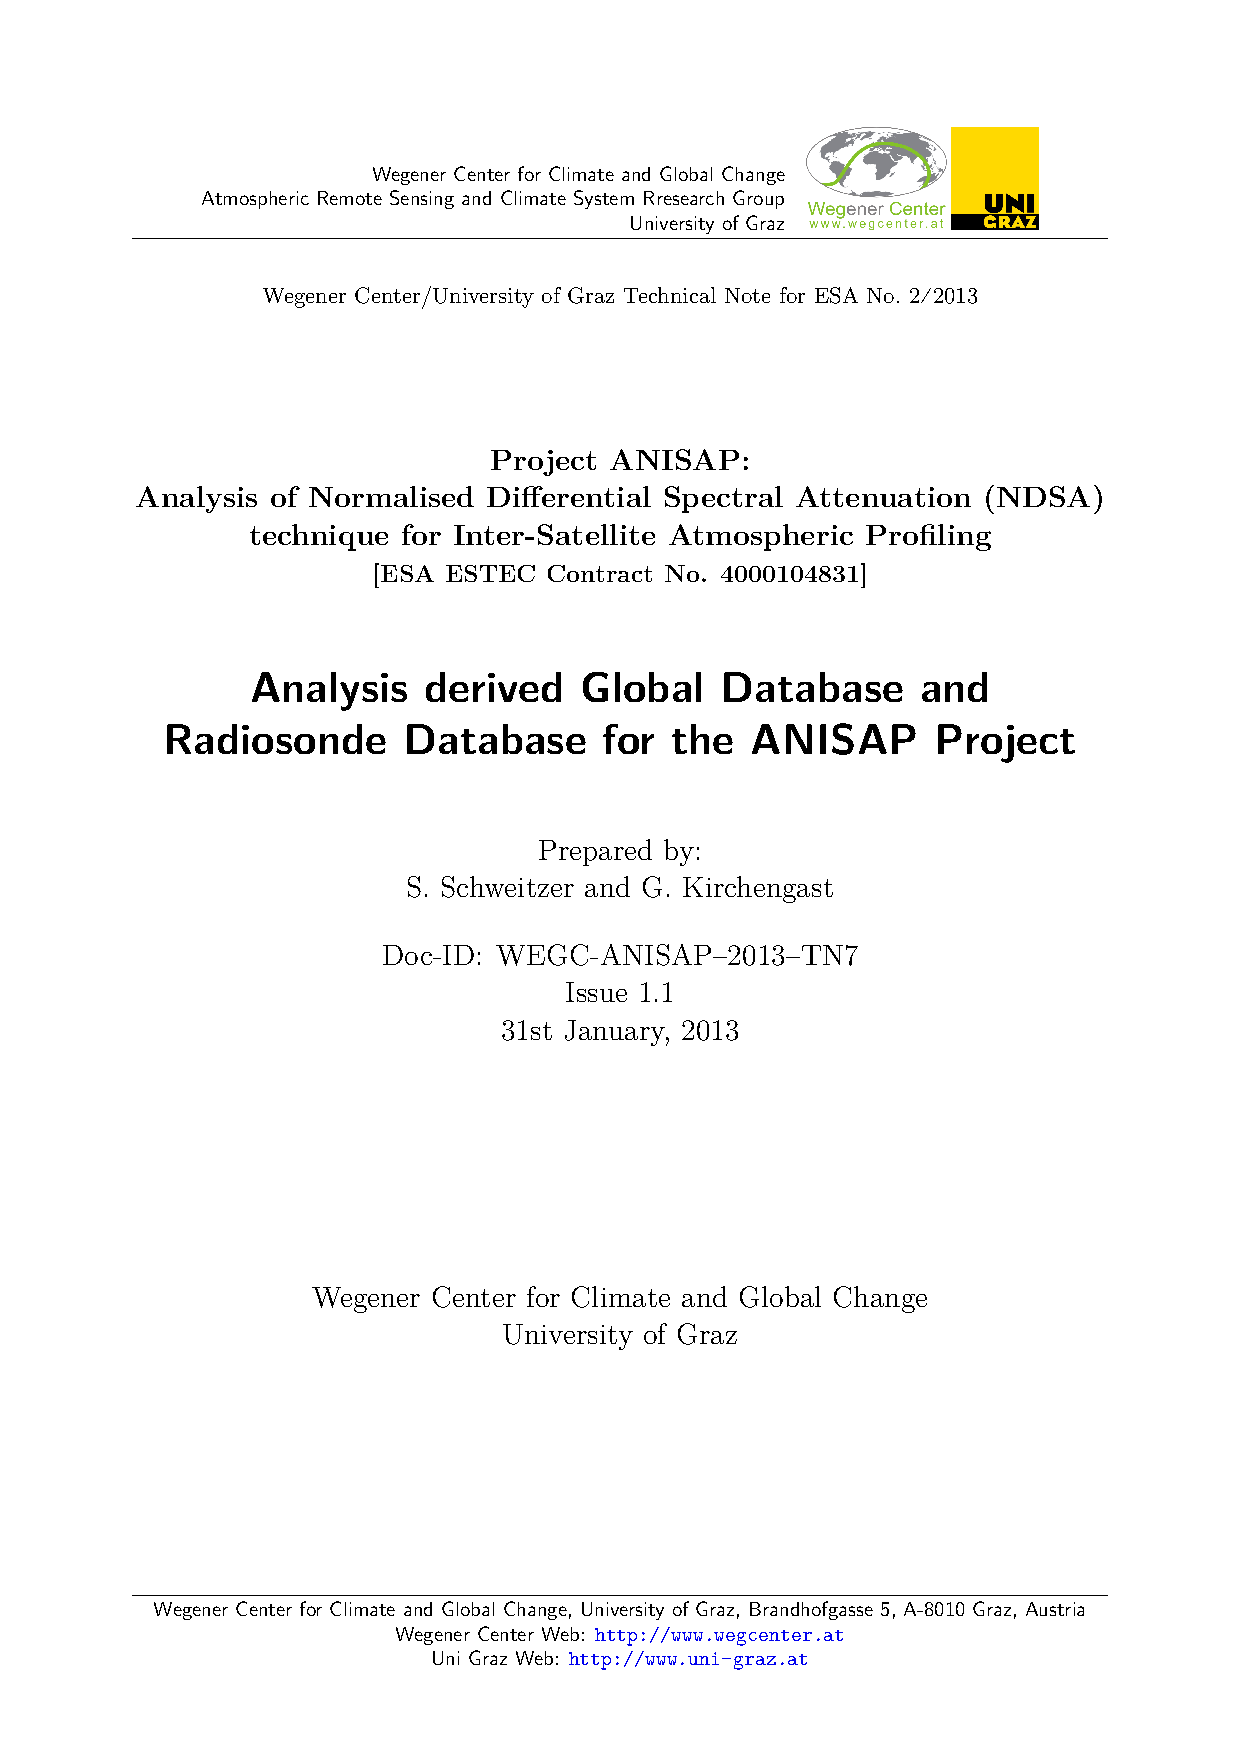
\includegraphics[height=0.7\paperheight, page=1]{anisap-TN2.pdf}}
  \caption{Example of a \multidoc document title page}
  \label{fig:multiDocTitlepage}
\end{figure}

\begin{figure}
  \centering
  \fbox{\includegraphics[height=0.7\paperheight, page=2]{anisap-TN2.pdf}}
  \caption{Example of a \multidoc document release information page}
  \label{fig:multiDocReleaseInfopage}
\end{figure}

\begin{figure}
  \centering
  \fbox{\includegraphics[height=0.7\paperheight, page=3]{anisap-TN2.pdf}}
  \caption{Example of a \multidoc document distribution list page}
  \label{fig:multiDocDistributionList}
\end{figure}

\begin{figure}
  \centering
  \fbox{\includegraphics[height=0.7\paperheight, page=4]{anisap-TN2.pdf}}
  \caption{Example of a \multidoc document change record page}
  \label{fig:multiDocChangeRecord}
\end{figure}

\begin{figure}
  \centering
  \fbox{\includegraphics[height=0.7\paperheight, page=10]{anisap-TN2.pdf}}
  \caption{Example of a \multidoc document random page}
  \label{fig:multiDocHeadings}
\end{figure}



\subsubsection[Document headings]{Tailoring the document headings}
\label{subsubsec:multiDocumentHeadings}

The layout of the document headings (\IE{} the header for the running
pages, see \autoref{fig:multiDocHeadings}) is the same for article, book
and report documents and is structured into three parts:
\begin{enumerate}
\item a four line text block on the left side (the exact definition of the
  concatenation of the string components is given in
  \autoref{lst:docstyleDocumentHeadingsTextBlock}) comprising
  \begin{enumerate}
  \item the document header title (built as a concatenated string from the
    document header title substring \latexcmd{\ThisDocHeaderTitleSubstr}
    and the document subtitle string \latexcmd{\ThisDocSubtitle}
  \item the document identifier (build as a concatenated string from the
    document identifier substring \latexcmd{\ThisDocIdSubstr}, the document
    release year \latexcmd{\ThisDocYear}, the document type%
    \footnote{The acronyms used for the various document types need to be
      defined in the file \path{acronyms.sty}, see
      \fullautoref{subsec:UsingTheAcronymDatabase}.}
    \latexcmd{\ThisDocType} (\EG{} \acs{tr} (\acl{tr}) or \acs{ar}
    (\acl{ar})), and the document internal number
    \latexcmd{\ThisDocIntNum})
  \item the document version (build as a concatenated string from the
    document issue number \latexcmd{\ThisDocIssue} and the document
    revision number \latexcmd{\ThisDocRevision}), and
  \item the document release date
  \end {enumerate}
\item a central single text line indicating the respective current section
  or chapter number and section or chapter title, and
\item a graphics block (of corporate logos) on the right side.
\end{enumerate}

The details and the structure of the document headings are defined in the
file \path{docstyle.sty} near line 315 to 354 (see
\autoref{lst:docstyleDocumentHeadings}).

Since individual details for a specific document from a \multidoc
documentation task are different from document to document due to the
different document content, document type, document identifiers, document
issue, document revision, document release date \ETC{}, these details are
only predefined in the file \path{docstyle.sty}, and intended to be
specifically tailored in each individual document's masterfile.

In essence, a block of redefining \LaTeX{} commands has to be added
(between the two already present commands \latexcmd{\makeatletter} and
\latexcmd{\makeatother}) to the master file, similar to the example given
in \autoref{lst:documentHeadingsExample}.
%
\begin{CommandLineListing}[style=DefaultFileListing, print=true, xleftmargin=0pt, gobble=2, %
  caption={Definition of document headings in the masterfile}, %
  label=lst:documentHeadingsExample]
  \makeatletter

  \renewcommand*{\ThisDocType}{%
    tr%
  }
  \renewcommand*{\ThisDocExtNum}{%
    03%
  }
  \renewcommand*{\ThisDocIntNum}{%
    37%
  }
  \renewcommand*{\ThisDocIssue}{%
    1%
  }
  \renewcommand*{\ThisDocRevision}{%
    3%
  }
  \renewcommand*{\subtitlePrefix}{%
    %
  }
  \renewcommand*{\ThisDocSubtitle}{%
    WLG Quickstart Guide%
  }
  \renewcommand*{\ThisDocHeaderTitleSubstr}{%
    \wegcLaTeX{}%
  }
  \renewcommand*{\ThisDocIdSubstr}{%
    \aces{wegc}-WLG-QSG%
  }
  \newdate{ThisDocDate}{13}{8}{2025}
  \renewcommand*{\ThisDocDate}{%
    \displaydate{ThisDocDate}%
  }
  \renewcommand*{\ThisDocYear}{%
    %% \getdateyear{ThisDocDate}%
    2028%
  }

  \makeatother
\end{CommandLineListing}

\lstinputlisting[style=DefaultFileListing, print=true,
   firstnumber=212, firstline=212, stepnumber=1, lastline=236,
   emptylines=*0,
   breaklines=true,
  caption={Definition of the documents headings text block in \texttt{\lstname}},
  label=lst:docstyleDocumentHeadingsTextBlock]{docstyle.sty}

\begin{landscape}
\lstinputlisting[style=DefaultFileListing, print=true,
   firstnumber=315, firstline=315, stepnumber=1, lastline=354,
   emptylines=*0,
   breaklines=true,
  caption={Definition of the document headings in \texttt{\lstname}},
  label=lst:docstyleDocumentHeadings]{docstyle.sty}
\end{landscape}


\subsubsection[Title page common elements]{Tailoring the common elements of the title page}
\label{subsubsec:multiDocumentTitlePageCommons}

The layout of the document title page is the same for article, book and
report documents and contains elements, which are common and the same for
all documents of a documentation task, \IE{} the title page header, the
title page footer, the document publisher details, the title head and the
subject details, and those that are different due to the individual
document content, \EG{} the document title or the document authors.


\minisec{Title page header and footer}

The common elements title page header and title page footer are defined and
specified in the file \path{docstyle.sty} near lines 252 and 271 (see
\autoref{lst:docstyleTitlepageHeaderFooter}).

\lstinputlisting[style=DefaultFileListing, print=true,
   firstnumber=252, firstline=252, stepnumber=1, lastline=281,
   emptylines=*1,
  caption={Definition of title page header and footer details in \texttt{\lstname}},
  label=lst:docstyleTitlepageHeaderFooter]{docstyle.sty}

If, for example, the combined \ac{igam}/\ac{wegc} title page header and
footer shall be replaced with the plain \ac{wegc} title page header and
footer, then the corresponding section in file \path{docstyle.sty} is to
be modified as shown in
\autoref{lst:docstyleTitlepageHeaderFooterWegcOnly}.
%
\begin{CommandLineListing}[style=DefaultFileListing, print=true, xleftmargin=0pt, gobble=2, %
  caption={Alternate definition of title page header and footer in \latexcmd{docstyle.sty}}, %
  label=lst:docstyleTitlepageHeaderFooterWegcOnly]
  \newcommand*{\Head@@ThisDocTitlePage}{%
    \upshape%
    \begin{varwidth}[b][0pt]{\paperwidth}%
      \LaTeXraggedleft%
      \Name{wegc}\\%
      %% \Name{igam}\\%
      \Name{ug}%
    \end{varwidth}%
    \quad%
    \begin{varwidth}[b][0pt]{\paperwidth}%
      
\includegraphics[height=50.0pt]{logo-ug-medium}%
      \hspace{2.0pt}%
      
\includegraphics[height=50.0pt]{logo-wegc-medium}%
      %% \hspace{2.0pt}%
      %% 
\includegraphics[height=50.0pt]{logo-igam-medium}%
    \end{varwidth}%
  }

  \newcommand*{\Foot@@ThisDocTitlePage}{%
    \upshape%
    \begin{varwidth}[t][0pt]{\paperwidth}%
      \LaTeXcentering%
      \Address{wegc}\\%
      %% \Address{igam}\\%
      \ShortName{wegc} Web\p: \WebAddress{wegc}\\%
      %% \ShortName{igam} Web\p: \WebAddress{igam}\\%
      \ShortName{ug} Web\p: \WebAddress{ug}\\%
    \end{varwidth}%
  }
\end{CommandLineListing}


\minisec{Title head and title subject details}

The title head and title subject details for the title page are defined in
the file \path{docstyle.sty} near lines 444 to 471 (see
\autoref{lst:docstyleTitlepageTitleheadSubject}).

\lstinputlisting[style=DefaultFileListing, print=true,
   firstnumber=444, firstline=444, stepnumber=1, lastline=471,
   emptylines=*0,
   caption={Definition of the title page title head and subject details in \texttt{\lstname}},
   label=lst:docstyleTitlepageTitleheadSubject]{docstyle.sty}

For changing the title page title head and subject details to something
different, the corresponding section in file \path{docstyle.sty} could
be modified as shown in
\autoref{lst:docstyleTitlepageTitleheadSubjectExample}.
%
\begin{CommandLineListing}[style=DefaultFileListing, print=true, xleftmargin=0pt, gobble=2, %
  caption={Alternate definition of title page title head and subject details in \latexcmd{docstyle.sty}}, %
  label=lst:docstyleTitlepageTitleheadSubjectExample]
  \newcommand*{\titleheadSubstr}{%
    \aces{wegc}%
  }
  \newcommand*{\titleheadSubSubstr}{%
    \aces{esa}%
  }
  \titlehead{%
    \makebox[\linewidth]{\titleheadSubstr \hbox{} \acel{\ThisDocType} for \titleheadSubSubstr \hbox{} \No{} \ThisDocExtNum\textfractionsolidus\ThisDocYear}%
  }
  \newcommand*{\subjectStr}{%
    rOPS Project\p:\\%
  }
  \newcommand*{\subjectSubstr}{%
    Typesetting and Document Generation%
  }
  \subject{%
    \subjectStr\subjectSubstr%
  }
\end{CommandLineListing}


\minisec{Publisher information}

The document publisher information for the title page is defined in the
file \path{docstyle.sty} near lines 504 to 520 (see
\autoref{lst:docstyleTitlepagePublisher}).

\lstinputlisting[style=DefaultFileListing, print=true,
   firstnumber=504, firstline=504, stepnumber=1, lastline=520,
   emptylines=*0,
   caption={Definition of the title page publisher details in \texttt{\lstname}},
   label=lst:docstyleTitlepagePublisher]{docstyle.sty}

For changing the title page publisher details to the plain \ac{wegc}
title page publisher details, the corresponding section in file
\path{docstyle.sty} is to be modified as shown in
\autoref{lst:docstyleTitlepagePublisherWegcOnly}.
%
\begin{CommandLineListing}[style=DefaultFileListing, print=true, xleftmargin=0pt, gobble=2, %
  caption={Alternate definition of title publisher details in \latexcmd{docstyle.sty}}, %
  label=lst:docstyleTitlepagePublisherWegcOnly]
  \newcommand*{\publishersSubstr}{%
    \acl{wegc}%
  }
  \newcommand*{\publishersSubSubstr}{%
    \acl{ug}%
  }
  \newcommand*{\publishersSubSubSubstr}{%
    %
  }
  \publishers{%
    \publishersSubstr\\\publishersSubSubstr\\\publishersSubSubSubstr%
  }
\end{CommandLineListing}


\minisec{Glossary and bibliography preambles}

If the default text for the preamble to the \emph{acronyms} and
\emph{abbreviations}, to the \emph{terms} and \emph{definitions}, or to the
bibliography does not fit as expected, these preambles can be modified in
\path{docstyle.sty}, starting near line 657 (see
\autoref{lst:docstyleGlossaryPreambles}) and near line 683 (see
\autoref{lst:docstyleBibliographyPreambles}).

\lstinputlisting[style=DefaultFileListing, print=true,
   firstnumber=657, firstline=657, stepnumber=1, lastline=670,
   emptylines=*0,
   caption={Definition of the glossary preambles in \texttt{\lstname}},
   label=lst:docstyleGlossaryPreambles]{docstyle.sty}

\lstinputlisting[style=DefaultFileListing, print=true,
   firstnumber=683, firstline=683, stepnumber=1, lastline=696,
   emptylines=*0,
   caption={Definition of the bibliography preambles in \texttt{\lstname}},
   label=lst:docstyleBibliographyPreambles]{docstyle.sty}


\subsubsection[Title page specific elements]{Tailoring the document specific elements of the title page}
\label{subsubsec:multiDocumentTitlePageSpecifics}

The layout of the document specific elements document title and authors are
predefined in the file \path{docstyle.sty} and need to be updated in each
individual document's masterfile by a block of redefining \LaTeX{} commands
which are to be added between the two already present commands
\latexcmd{\makeatletter} and \latexcmd{\makeatother}, similar to the
example given in \autoref{lst:documenTitlepageTitleExample}.

All other document specific elements required for the title page like
document type, document identifiers, document issue, document revision,
document release date \ETC{}, have already been described for the document
headings in \autoref{subsubsec:multiDocumentHeadings}

\Attention{%
  In \autoref{lst:documenTitlepageTitleExample}, the definition of the
  document subtitle is not explicitly shown, as it is already presented in
  \autoref{lst:documentHeadingsExample} of
  \autoref{subsubsec:multiDocumentHeadings} (due to the fact that
  \latexcmd{\subtitlePrefix} and \latexcmd{\ThisDocSubtitle} are used for
  the definition of the document headings).}

\begin{CommandLineListing}[style=DefaultFileListing, print=true, xleftmargin=0pt, gobble=2, %
  caption={Definition of document title and author details in the masterfile}, %
  label=lst:documenTitlepageTitleExample]
  \makeatletter
  ...
  ...
  \renewcommand*{\ThisDocTitle}{%
    The \wegcLaTeX{} documentation framework: \newline a guide for beginners%
  }
  \renewcommand*{\titlePrefix}{%
    %
  }
  \renewcommand*{\ThisDocAuthors}{%
    \ShortName{kmf}, \ShortName{jfb}, and \ShortName{gki}%
  }
  \makeatother
\end{CommandLineListing}


\subsubsection[A \multidoc document article]{Creating a \multidoc document article}
\label{subsubsec:creatingMultiDocumentArticle}

For creating a \multidoc article, proceed as follows:
%%
\begin{enumerate}
\item create a working directory for building the \wegcLaTeX{} \multidoc article, \\
  \EG{} \path{/home/\plh{user}/wlMultiDocTest/}

\item create the following subdirectories \\
  \path{/home/\plh{user}/wlMultiDocTest/wlg/}, \\
  \path{/home/\plh{user}/wlMultiDocTest/wlg/figs/}, \\
  \path{/home/\plh{user}/wlMultiDocTest/wlg/data/}, \\
  \path{/home/\plh{user}/wlMultiDocTest/wlg/tex/}, \\
  \path{/home/\plh{user}/wlMultiDocTest/common/}, and \\
  \path{/home/\plh{user}/wlMultiDocTest/common/figs}

  \Attention{Any further documents of a \multidoc documentation task would
    require the additional subdirectories \\
    \path{/home/\plh{user}/wlMultiDocTest/wlg2/}, \\
    \path{/home/\plh{user}/wlMultiDocTest/wlg2/figs/}, \\
    \path{/home/\plh{user}/wlMultiDocTest/wlg2/data/}, \\
    \path{/home/\plh{user}/wlMultiDocTest/wlg2/tex/}, \\
    and so on.}

\item copy the \LaTeX{} template master file \\
  \path{./texmf/doc/latex/wegc-latex/examples/multidoc-article/doc-article.tex} to \\
  \path{/home/\plh{user}/wlMultiDocTest/wlg/}

\item copy the seven \LaTeX{} source code files from \\
  \path{./texmf/doc/latex/wegc-latex/WLG/} to \\
  \path{/home/\plh{user}/wlMultiDocTest/wlg/tex/}

\item copy the twelve \path{*.png} and twelve \path{*.xbb} files from \\
  \path{./texmf/doc/latex/wegc-latex/examples/common/figs/} to \\
  \path{/home/\plh{user}/wlMultiDocTest/common/figs/}

\item copy the three files
  \path{docstyle.sty}, \path{project.sty}, and \path{commands.sty} from \\
  \path{./texmf/doc/latex/wegc-latex/examples/common/} to \\
  \path{/home/\plh{user}/wlMultiDocTest/common}

 \item extract the three example only files \path{acronyms.sty}, \path{addresses.sty}, and
  \path{terms.sty} from the compressed archive file \\
  \path{./texmf/doc/latex/wegc-latex/WLG/acronymsAddressesTerms_ExampleDoNotUse.tar.gz}
  or use the current and up to date versions available at 
  \nolinkurl{https://wegc203117.uni-graz.at/projects/latex_dbs/browser/arsclisys}
  and put them to \\
  \path{/home/\plh{user}/wlMultiDocTest/common}

\item add the address for the fictive person ``\Name{kmf}'' at the end of
  the copied file \path{addresses.sty}, as described in
  \autoref{subsec:usingTheAddressBookDatabase}

\item add the acronym for the fictive company ``\acf{tmc}'' at the end of
  the copied file \path{acronyms.sty}, as described in
  \autoref{subsec:UsingTheAcronymDatabase}

\item add the glossary entry for the fictive term ``\Gls{firlefanzation}''
  at the end of the copied file \path{terms.sty}, as described in
  \autoref{subsec:UsingTheGlossaryDatabase}

\item create an example bibliography file \path{exampleBibFile.bib} in the \\
  \path{/home/\plh{user}/wlMultiDocTest/wlg} directory in the same way as
  it is described for a \singledoc article (see
  \autoref{subsubsec:creatingSingleDocumentArticle})

\item copy the template master file \\
  \path{/home/\plh{user}/wlMultiDocTest/wlg/doc-wlarticle.tex} to \\
  \path{/home/\plh{user}/wlMultiDocTest/wlg/md-wlgArticle.tex} \\
  and apply the following modifications:
  \begin{enumerate}
  \item at line 119, change \latexcmd{DIV=default} to \latexcmd{DIV=11}
  \item between the lines 165 to 171, reading
    \begin{CommandLineListing}[style=DefaultFileListing, print=true, basicstyle={\ttfamily\small}, %
      basewidth=0.47em, xleftmargin=0pt, gobble=6]
      \makeatletter
      %% NOTE: Here, we can act as class and package authors if we want or need to do so ...
      \makeatother
    \end{CommandLineListing}
    add the definition commands for defining the document specific settings:
    \begin{CommandLineListing}[style=DefaultFileListing, print=true, basicstyle={\ttfamily\small}, %
      basewidth=0.47em, xleftmargin=0pt, gobble=6]
      \makeatletter

      \renewcommand*{\ThisDocType}{%
        tr%
      }
      \renewcommand*{\ThisDocExtNum}{%
        03%
      }
      \renewcommand*{\ThisDocIntNum}{%
        37%
      }
      \renewcommand*{\ThisDocIssue}{%
        1%
      }
      \renewcommand*{\ThisDocRevision}{%
        3%
      }
      \renewcommand*{\subtitlePrefix}{%
        %
      }
      \renewcommand*{\ThisDocSubtitle}{%
        WLG Quickstart Guide%
      }
      \renewcommand*{\ThisDocHeaderTitleSubstr}{%
        \wegcLaTeX{}%
      }
      \renewcommand*{\ThisDocIdSubstr}{%
        \aces{wegc}-WLG-QSG%
      }
      \newdate{ThisDocDate}{13}{8}{2025}
      \renewcommand*{\ThisDocDate}{%
        \displaydate{ThisDocDate}%
      }
      \renewcommand*{\ThisDocYear}{%
        %% \getdateyear{ThisDocDate}%
        2028%
      }
      \renewcommand*{\ThisDocTitle}{%
        The \wegcLaTeX{} documentation framework: \newline a guide for beginners%
      }
      \renewcommand*{\titlePrefix}{%
        %
      }
      \renewcommand*{\ThisDocAuthors}{%
        \ShortName{kmf}, \ShortName{jfb}, and \ShortName{gki}%
      }
      \makeatother
    \end{CommandLineListing}

  \item on lines 150 to 151: change from
    \begin{CommandLineListing}[style=DefaultFileListing, print=true, basicstyle={\ttfamily\small}, %
      basewidth=0.47em, xleftmargin=0pt, gobble=6]
      \bibliography{%
      }
    \end{CommandLineListing}
    to
    \begin{CommandLineListing}[style=DefaultFileListing, print=true, basicstyle={\ttfamily\small}, %
      basewidth=0.47em, xleftmargin=0pt, gobble=6]
      \bibliography{%
        exampleBibFile%
      }
    \end{CommandLineListing}

  \item between lines 165 and 171, reading
    \begin{CommandLineListing}[style=DefaultFileListing, print=true, basicstyle={\ttfamily\small}, %
      basewidth=0.47em, xleftmargin=0pt, gobble=6]
      \makeatletter

      %% NOTE: Here, we can act as class and package authors if we want or need to do so ...

      \makeatother
    \end{CommandLineListing}
    add the following command definitiosn for \entity{singledoc} and \entity{multidoc}:
    \begin{CommandLineListing}[style=DefaultFileListing, print=true, basicstyle={\ttfamily\small}, %
      basewidth=0.47em, xleftmargin=0pt, gobble=6]
      \makeatletter

      %% NOTE: Here, we can act as class and package authors if we want or need to do so ...

      \newcommand*{\singledoc}{%
        \entity{singledoc} %
      }

      \newcommand*{\multidoc}{%
        \entity{multidoc} %
      }

      \makeatother
    \end{CommandLineListing}

  \item \label{item:nociteGlsaddIncludeDirectives} between the lines 201
    and 204, reading
    \begin{CommandLineListing}[style=DefaultFileListing, print=true, basicstyle={\ttfamily\small}, %
      basewidth=0.47em, xleftmargin=0pt, gobble=6]
      \printbibliography[prenote=refpreamble]


      \appendix
    \end{CommandLineListing}
    add the following content:
    \begin{CommandLineListing}[style=DefaultFileListing, print=true, basicstyle={\ttfamily\small}, %
      basewidth=0.47em, xleftmargin=0pt, gobble=6]
      \printbibliography[prenote=refpreamble]

      \nocite{Gorbunov2007a}
      \nocite{Gorbunov2002a}
      \nocite{Gorbunov1986}

      \glsadd{development_team}
      \glsadd{firlefanzation}

      \glsadd{urd}
      \glsadd{add}
      \glsadd{ddd}
      \glsadd{sum}
      \glsadd{atr}

      \include{WLG-1_introduction}
      \include{WLG-2_installation}
      \include{WLG-3_documentGeneration}
      \include{WLG-4_commandsAndEnvironments}
      \include{WLG-5_practicalTips}
      \include{WLG-6_usingTheTemplates}
      \include{WLG-7_undocumentedTopics}

      \appendix
    \end{CommandLineListing}
   \end{enumerate}

 \item modify in the file
   \path{/home/\plh{user}/wlMultiDocTest/common/docstyle.sty} the titlepage
   header, titlepage footer, titlehead, subject and publisher details as
   described in \autoref{subsubsec:multiDocumentTitlePageCommons}.

 \item Finally, compile the master file
   \path{/home/\plh{user}/wlMultiDocTest/wlg/md-wlgArticle.tex} as
   described in \autoref{subsec:commandsForDocumentGeneration}.
\end{enumerate}


\subsubsection[A \multidoc document report]{Creating a \multidoc document report}
\label{subsubsec:creatingMultiDocumentReport}

For creating a \multidoc report, copy the \LaTeX{} template master file \\
\path{./texmf/doc/latex/wegc-latex/examples/multidoc-report/doc-report.tex} to \\
\path{/home/\plh{user}/wlMultiDocTest/wlg/}, \\
copy the file \\
\path{/home/\plh{user}/wlMultiDocTest/wlg/doc-wlreport.tex} to \\
\path{/home/\plh{user}/wlMultiDocTest/wlg/md-wlgReport.tex}, \\
and perform all other steps similar to the description in
\autoref{subsubsec:creatingMultiDocumentArticle}, considering the following
differences:
%%
\begin{enumerate}

\item in file \path{/home/\plh{user}/wlMultiDocTest/wlg/md-wlgReport.tex},
  \begin{enumerate}
  \item \label{item:nociteGlsaddIncludeMdReport} between the lines 213 and
    216 (\IE{} between the \latexcmd{\printbibliography} and
    \latexcmd{\appendix} commands), add the same \LaTeX{} commands
    \latexcmd{\nocite}, \latexcmd{\glsadd} and \latexcmd{\include} as
    indicated in \autoref{subsubsec:creatingMultiDocumentArticle},
    \autoref{item:nociteGlsaddIncludeDirectives}

  \item between the lines 213 and 216 (\IE{} between the
    \latexcmd{\printbibliography} and \latexcmd{\appendix} commands and
    immediately after the added statements of
    \autoref{item:nociteGlsaddIncludeMdReport}), add the definition of the
    \entity{Document Release Information} table, the \entity{Document
      Distribution List} and the \entity{Document Change Record}, as shown
    in \autoref{lst:exampleReleaseDistributionChangeRecord}
  \end{enumerate}

\item modify the document structuring directives \latexcmd{\section},
  \latexcmd{\subsection} and \latexcmd{\subsubsection} used in the seven
  \LaTeX{} files to \latexcmd{\chapter}, \latexcmd{\section} and
  \latexcmd{\subsection}, adapting it to the proper sectioning for report
  documents (similar to \autoref{subsubsec:creatingSingleDocumentReport}
  \autoref{item:modifyStructuringDirectives}).

\item Finally, compile the master file
  \path{/home/\plh{user}/wlMultiDocTest/wlg/md-wlgReport.tex} as described
  in \autoref{subsec:commandsForDocumentGeneration}.

\end{enumerate}


\begin{CommandLineListing}[style=DefaultFileListing, print=true, basicstyle={\ttfamily\small}, %
  basewidth=0.47em, xleftmargin=0pt, gobble=2, %
  caption={Definition of document release information, distribution list and change record}, %
  label=lst:exampleReleaseDistributionChangeRecord]
  \renewcommand*{\ThisAuthorizationIdentity}{%
    \ShortName{mip}, \ugorg{short}%
  }

  \renewcommand*{\ThisApprovalIdentity}{%
    \ShortName{gki}, \ugorg{short}%
  }

  %% \renewcommand*{\ThisDocReleaseInformationTab}{%
  %% \ifthenelse{\boolean{KOMAClass}}{\addsec*}{\section*}{Document Release Information}%
  %% \begin{tabularx}{\linewidth}[b]{@{}D@{}}%
  %%   \toprule%
  %%   \docid                                      & \ThisDocId                  \\%
  %%   Issue                                       & \ThisDocVersion             \\%
  %%   Date                                        & \ThisDocDate                \\%
  %%   Prepared by                                 & \ThisDocAuthors             \\%
  %%   Approved\textfractionsolidus{}Internally by & \ThisAuthorizationIdentity  \\%
  %%   Approved\textfractionsolidus{}Externally by & \ThisApprovalIdentity       \\%
  %%   \bottomrule%
  %% \end{tabularx}%
  %% }

  \renewcommand*{\ThisDocDistributionList}{%
    \ShortName{gki}       &  \aces{wegc}/\aces{ug}    & \EmailAddress{gki}       & 1\\%
    \small\ShortName{jfb} &  \aces{wegc}/\aces{ug}    & \small\EmailAddress{jfb} & 1\\%
    \Name{mip}            &  \aces{wegc}/\aces{ug}    & \EmailAddress{mip}       & 1%
  }

  \renewcommand*{\ThisDocChangeRecord}{%
    \software{short}{Version}{1}{0}{}{} &%
    \formatdate{20}{04}{2007} &%
    Original version of the document\p. \\ %
    %%
    \software{short}{Version}{1}{2}{}{} &%
    \formatdate{21}{12}{2008} &%
    Updates throughout the document by minor \newline
    changes and editorial corrections for clarification\p. \\ %
    %%
    \software{short}{Version}{\ThisDocIssue}{\ThisDocRevision}{}{}  &%
    \ThisDocDate &%
    Correction of minor inconsistencies\p.%
  }
\end{CommandLineListing}



\subsubsection[A \multidoc document book]{Creating a \multidoc document book}
\label{subsubsec:creatingMultiDocumentBook}

For creating a \multidoc book, copy the \LaTeX{} template master file \\
\path{./texmf/doc/latex/wegc-latex/examples/multidoc-book/doc-wlbook.tex} to \\
\path{/home/\plh{user}/wlMultiDocTest/wlg/}, copy the file \\
\path{/home/\plh{user}/wlMultiDocTest/wlg/doc-wlbook.tex} to \\
\path{/home/\plh{user}/wlMultiDocTest/wlg/md-wlgBook.tex} 
and perform all other steps similar to the description in
\autoref{subsubsec:creatingMultiDocumentArticle}, considering the following
differences:
%%
\begin{enumerate}

\item in file \path{/home/\plh{user}/wlMultiDocTest/wlg/md-wlgBook.tex},
  \begin{enumerate}
  \item \label{item:nociteGlsaddIncludeMdBook} between the lines 219 and
    222 (\IE{} between the \latexcmd{\mainmatter} and \latexcmd{\appendix}
    commands), add the same \LaTeX{} commands \latexcmd{\nocite},
    \latexcmd{\glsadd} and \latexcmd{\include} as indicated in
    \autoref{subsubsec:creatingMultiDocumentArticle},
    \autoref{item:nociteGlsaddIncludeDirectives}

  \item between the lines 219 and 222 (\IE{} between the
    \latexcmd{\mainmatter} and \latexcmd{\appendix} commands and
    immediately after the added statements of
    \autoref{item:nociteGlsaddIncludeMdBook}), add the definition of the
    \entity{Document Release Information} table, the \entity{Document
      Distribution List} and the \entity{Document Change Record}, as shown
    in \autoref{lst:exampleReleaseDistributionChangeRecord}
  \end{enumerate}

\item modify the document structuring directives \latexcmd{\section},
  \latexcmd{\subsection} and \latexcmd{\subsubsection} used in the seven
  \LaTeX{} files to \latexcmd{\chapter}, \latexcmd{\section} and
  \latexcmd{\subsection}, adapting it to the proper sectioning for book
  documents (similar to \autoref{subsubsec:creatingSingleDocumentReport}
  \autoref{item:modifyStructuringDirectives}).

\item Finally, compile the master file \\
  \path{/home/\plh{user}/wlMultiDocTest/wlg/md-wlgBook.tex} \\
  as described in \autoref{subsec:commandsForDocumentGeneration}.

\end{enumerate}

      


\section[Undocumented topics]{Undocumented topics}

Additionally, the following features are provided as an extension to the \KOMAScript{} bundle:
%
\begin{itemize}
   \item \latexcmd{\rowstyle} and column types \entity{=}, \entity{+}
   \item column type \entity{D}
   \item \latexcmd{\noacronymfont} (\entity{glossaries} package)
   \item \latexcmd{\acrentryshort} (\entity{glossaries} package) and similar commands + shortcuts
\end{itemize}

\noindent{}TODO Describe all packages loaded in \wegcLaTeX{}: What are they
for, basic functionality, basic commands.



      \appendix
    \end{CommandLineListing}
   \end{enumerate}

 \item modify in the file
   \path{/home/\plh{user}/wlMultiDocTest/common/docstyle.sty} the titlepage
   header, titlepage footer, titlehead, subject and publisher details as
   described in \autoref{subsubsec:multiDocumentTitlePageCommons}.

 \item Finally, compile the master file
   \path{/home/\plh{user}/wlMultiDocTest/wlg/md-wlgArticle.tex} as
   described in \autoref{subsec:commandsForDocumentGeneration}.
\end{enumerate}


\subsubsection[A \multidoc document report]{Creating a \multidoc document report}
\label{subsubsec:creatingMultiDocumentReport}

For creating a \multidoc report, copy the \LaTeX{} template master file \\
\path{./texmf/doc/latex/wegc-latex/examples/multidoc-report/doc-report.tex} to \\
\path{/home/\plh{user}/wlMultiDocTest/wlg/}, \\
copy the file \\
\path{/home/\plh{user}/wlMultiDocTest/wlg/doc-wlreport.tex} to \\
\path{/home/\plh{user}/wlMultiDocTest/wlg/md-wlgReport.tex}, \\
and perform all other steps similar to the description in
\autoref{subsubsec:creatingMultiDocumentArticle}, considering the following
differences:
%%
\begin{enumerate}

\item in file \path{/home/\plh{user}/wlMultiDocTest/wlg/md-wlgReport.tex},
  \begin{enumerate}
  \item \label{item:nociteGlsaddIncludeMdReport} between the lines 213 and
    216 (\IE{} between the \latexcmd{\printbibliography} and
    \latexcmd{\appendix} commands), add the same \LaTeX{} commands
    \latexcmd{\nocite}, \latexcmd{\glsadd} and \latexcmd{\include} as
    indicated in \autoref{subsubsec:creatingMultiDocumentArticle},
    \autoref{item:nociteGlsaddIncludeDirectives}

  \item between the lines 213 and 216 (\IE{} between the
    \latexcmd{\printbibliography} and \latexcmd{\appendix} commands and
    immediately after the added statements of
    \autoref{item:nociteGlsaddIncludeMdReport}), add the definition of the
    \entity{Document Release Information} table, the \entity{Document
      Distribution List} and the \entity{Document Change Record}, as shown
    in \autoref{lst:exampleReleaseDistributionChangeRecord}
  \end{enumerate}

\item modify the document structuring directives \latexcmd{\section},
  \latexcmd{\subsection} and \latexcmd{\subsubsection} used in the seven
  \LaTeX{} files to \latexcmd{\chapter}, \latexcmd{\section} and
  \latexcmd{\subsection}, adapting it to the proper sectioning for report
  documents (similar to \autoref{subsubsec:creatingSingleDocumentReport}
  \autoref{item:modifyStructuringDirectives}).

\item Finally, compile the master file
  \path{/home/\plh{user}/wlMultiDocTest/wlg/md-wlgReport.tex} as described
  in \autoref{subsec:commandsForDocumentGeneration}.

\end{enumerate}


\begin{CommandLineListing}[style=DefaultFileListing, print=true, basicstyle={\ttfamily\small}, %
  basewidth=0.47em, xleftmargin=0pt, gobble=2, %
  caption={Definition of document release information, distribution list and change record}, %
  label=lst:exampleReleaseDistributionChangeRecord]
  \renewcommand*{\ThisAuthorizationIdentity}{%
    \ShortName{mip}, \ugorg{short}%
  }

  \renewcommand*{\ThisApprovalIdentity}{%
    \ShortName{gki}, \ugorg{short}%
  }

  %% \renewcommand*{\ThisDocReleaseInformationTab}{%
  %% \ifthenelse{\boolean{KOMAClass}}{\addsec*}{\section*}{Document Release Information}%
  %% \begin{tabularx}{\linewidth}[b]{@{}D@{}}%
  %%   \toprule%
  %%   \docid                                      & \ThisDocId                  \\%
  %%   Issue                                       & \ThisDocVersion             \\%
  %%   Date                                        & \ThisDocDate                \\%
  %%   Prepared by                                 & \ThisDocAuthors             \\%
  %%   Approved\textfractionsolidus{}Internally by & \ThisAuthorizationIdentity  \\%
  %%   Approved\textfractionsolidus{}Externally by & \ThisApprovalIdentity       \\%
  %%   \bottomrule%
  %% \end{tabularx}%
  %% }

  \renewcommand*{\ThisDocDistributionList}{%
    \ShortName{gki}       &  \aces{wegc}/\aces{ug}    & \EmailAddress{gki}       & 1\\%
    \small\ShortName{jfb} &  \aces{wegc}/\aces{ug}    & \small\EmailAddress{jfb} & 1\\%
    \Name{mip}            &  \aces{wegc}/\aces{ug}    & \EmailAddress{mip}       & 1%
  }

  \renewcommand*{\ThisDocChangeRecord}{%
    \software{short}{Version}{1}{0}{}{} &%
    \formatdate{20}{04}{2007} &%
    Original version of the document\p. \\ %
    %%
    \software{short}{Version}{1}{2}{}{} &%
    \formatdate{21}{12}{2008} &%
    Updates throughout the document by minor \newline
    changes and editorial corrections for clarification\p. \\ %
    %%
    \software{short}{Version}{\ThisDocIssue}{\ThisDocRevision}{}{}  &%
    \ThisDocDate &%
    Correction of minor inconsistencies\p.%
  }
\end{CommandLineListing}



\subsubsection[A \multidoc document book]{Creating a \multidoc document book}
\label{subsubsec:creatingMultiDocumentBook}

For creating a \multidoc book, copy the \LaTeX{} template master file \\
\path{./texmf/doc/latex/wegc-latex/examples/multidoc-book/doc-wlbook.tex} to \\
\path{/home/\plh{user}/wlMultiDocTest/wlg/}, copy the file \\
\path{/home/\plh{user}/wlMultiDocTest/wlg/doc-wlbook.tex} to \\
\path{/home/\plh{user}/wlMultiDocTest/wlg/md-wlgBook.tex} 
and perform all other steps similar to the description in
\autoref{subsubsec:creatingMultiDocumentArticle}, considering the following
differences:
%%
\begin{enumerate}

\item in file \path{/home/\plh{user}/wlMultiDocTest/wlg/md-wlgBook.tex},
  \begin{enumerate}
  \item \label{item:nociteGlsaddIncludeMdBook} between the lines 219 and
    222 (\IE{} between the \latexcmd{\mainmatter} and \latexcmd{\appendix}
    commands), add the same \LaTeX{} commands \latexcmd{\nocite},
    \latexcmd{\glsadd} and \latexcmd{\include} as indicated in
    \autoref{subsubsec:creatingMultiDocumentArticle},
    \autoref{item:nociteGlsaddIncludeDirectives}

  \item between the lines 219 and 222 (\IE{} between the
    \latexcmd{\mainmatter} and \latexcmd{\appendix} commands and
    immediately after the added statements of
    \autoref{item:nociteGlsaddIncludeMdBook}), add the definition of the
    \entity{Document Release Information} table, the \entity{Document
      Distribution List} and the \entity{Document Change Record}, as shown
    in \autoref{lst:exampleReleaseDistributionChangeRecord}
  \end{enumerate}

\item modify the document structuring directives \latexcmd{\section},
  \latexcmd{\subsection} and \latexcmd{\subsubsection} used in the seven
  \LaTeX{} files to \latexcmd{\chapter}, \latexcmd{\section} and
  \latexcmd{\subsection}, adapting it to the proper sectioning for book
  documents (similar to \autoref{subsubsec:creatingSingleDocumentReport}
  \autoref{item:modifyStructuringDirectives}).

\item Finally, compile the master file \\
  \path{/home/\plh{user}/wlMultiDocTest/wlg/md-wlgBook.tex} \\
  as described in \autoref{subsec:commandsForDocumentGeneration}.

\end{enumerate}

      


\section[Undocumented topics]{Undocumented topics}

Additionally, the following features are provided as an extension to the \KOMAScript{} bundle:
%
\begin{itemize}
   \item \latexcmd{\rowstyle} and column types \entity{=}, \entity{+}
   \item column type \entity{D}
   \item \latexcmd{\noacronymfont} (\entity{glossaries} package)
   \item \latexcmd{\acrentryshort} (\entity{glossaries} package) and similar commands + shortcuts
\end{itemize}

\noindent{}TODO Describe all packages loaded in \wegcLaTeX{}: What are they
for, basic functionality, basic commands.



      \appendix
    \end{CommandLineListing}

  \item near the lines 135, directly after the \latexcmd{\documentclass}
    directive, add the following commands:
    \begin{CommandLineListing}[style=DefaultFileListing, print=true, basicstyle={\ttfamily\small}, %
      basewidth=0.47em, xleftmargin=0pt, gobble=6]
      \RequirePackage{acronyms}
      \RequirePackage{terms}
      \RequirePackage{addresses}
      \RequirePackage{commands}
    \end{CommandLineListing}

  \end{enumerate}

\item Finally, compile the master file \\
  \path{/home/\plh{user}/wlSingleDocTest/wlg/wlgArticle.tex} \\
  as described in \autoref{subsec:commandsForDocumentGeneration}.
\end{enumerate}


\subsubsection[A \singledoc document report]{Creating a \singledoc document report}
\label{subsubsec:creatingSingleDocumentReport}

For creating a \singledoc report, copy the \LaTeX{} template master file \\
\path{./texmf/doc/latex/wegc-latex/examples/singledoc/master-wlreport.tex} to \\
\path{/home/\plh{user}/wlSingleDocTest/wlg/}. \\
Then copy the file \\
\path{/home/\plh{user}/wlSingleDocTest/wlg/master-wlreport.tex} to \\
\path{/home/\plh{user}/wlSingleDocTest/wlg/wlgReport.tex} \\
and perform all other steps similar to the description in
\autoref{subsubsec:creatingSingleDocumentArticle}, considering the
following differences:
%%
\begin{enumerate}
\item change the setting for \latexcmd{\extratitle},
  \latexcmd{\uppertitleback}, and \latexcmd{\lowertitleback} from
  \begin{CommandLineListing}[style=DefaultFileListing, print=true, basicstyle={\ttfamily\small}, %
    basewidth=0.47em, xleftmargin=0pt, gobble=4]
    \extratitle{%
      \highlight{\placeholder{My Bastard Title}}%
    }
    \uppertitleback{%
      \highlight{\placeholder{My Upper Title Back}}%
    }
    \lowertitleback{%
      \highlight{\placeholder{My Lower Title Back}}%
    }
  \end{CommandLineListing}
  to
  \begin{CommandLineListing}[style=DefaultFileListing, print=true, basicstyle={\ttfamily\small}, %
    basewidth=0.47em, xleftmargin=0pt, gobble=4]
    \extratitle{%
      %
    }
    \uppertitleback{%
      %
    }
    \lowertitleback{%
      %
    }
  \end{CommandLineListing}
  or to specific texts fitting the intended publication.

\item
  instead of
  \begin{CommandLineListing}[style=DefaultFileListing, print=true, basicstyle={\ttfamily\small}, %
    basewidth=0.47em, xleftmargin=0pt, gobble=4]
    \defbibnote{refpreamble}{%
      \highlight{\placeholder{My References Preamble}}%
    }
  \end{CommandLineListing}
  change it to
  \begin{CommandLineListing}[style=DefaultFileListing, print=true, basicstyle={\ttfamily\small}, %
    basewidth=0.47em, xleftmargin=0pt, gobble=4]
    \defbibnote{bibpreamble}{%
      %
    }
  \end{CommandLineListing}
  or to a specific text appropriate for the intended publication.

\item \label{item:modifyStructuringDirectives}
  modify the document structuring directives \latexcmd{\section},
  \latexcmd{\subsection} and \latexcmd{\subsubsection}
  used within the files \\
  \path{WLG-1_introduction}, \\
  \path{WLG-2_installation}, \\
  \path{WLG-3_documentGeneration}, \\
  \path{WLG-4_commandsAndEnvironments}, \\
  \path{WLG-5_practicalTips}, \\
  \path{WLG-6_usingTheTemplates}, and \\
  \path{WLG-7_undocumentedTopics} to \\
  \latexcmd{\chapter}, \latexcmd{\section} and \latexcmd{\subsection},
  adapting it to the proper sectioning for report documents.

\item place the \latexcmd{\include} directives for including the seven
  \LaTeX{} subdocument files between the \latexcmd{\printglossary} and
  \latexcmd{\appendix} commands.

\item Finally, compile the master file \path{wlgReport.tex} as described in
  \autoref{subsec:commandsForDocumentGeneration}.
\end{enumerate}



\subsubsection[A \singledoc document book]{Creating a \singledoc document book}
\label{subsubsec:creatingSingleDocumentBook}

For creating a \singledoc book, copy the \LaTeX{} template master file \\
\path{./texmf/doc/latex/wegc-latex/examples/singledoc/master-wlbook.tex} to \\
\path{/home/\plh{user}/wlSingleDocTest/wlg/}. \\
Then copy the file \\
\path{/home/\plh{user}/wlSingleDocTest/wlg/master-wlbook.tex} to \\
\path{/home/\plh{user}/wlSingleDocTest/wlg/wlgBook.tex} \\
and perform all other steps similar to the description in
\autoref{subsubsec:creatingSingleDocumentArticle}, considering the following differences:
%%
\begin{enumerate}
\item change the settings for \latexcmd{\extratitle},
  \latexcmd{\uppertitleback}, \latexcmd{\lowertitleback},\\
  \latexcmd{\upperinfopage}, \latexcmd{\lowerinfopage}, and
  \latexcmd{\lastpage} from
  \begin{CommandLineListing}[style=DefaultFileListing, print=true, basicstyle={\ttfamily\small}, %
    basewidth=0.47em, xleftmargin=0pt, gobble=4]
    \extratitle{%
      \highlight{\placeholder{My Bastard Title}}%
    }
    \uppertitleback{%
      \highlight{\placeholder{My Upper Title Back}}%
    }
    \lowertitleback{%
      \highlight{\placeholder{My Lower Title Back}}%
    }
    \upperinfopage{%
      \highlight{\placeholder{My Upper Info Page}}%
    }
    \lowerinfopage{%
      \highlight{\placeholder{My Lower Info Page}}%
    }
    \lastpage{%
      \highlight{\placeholder{My Last Page}}%
    }
  \end{CommandLineListing}
  to
  \begin{CommandLineListing}[style=DefaultFileListing, print=true, basicstyle={\ttfamily\small}, %
    basewidth=0.47em, xleftmargin=0pt, gobble=4]
    \extratitle{%
      %
    }
    \uppertitleback{%
      %
    }
    \lowertitleback{%
      %
    }
    \upperinfopage{%
      %
    }
    \lowerinfopage{%
      %
    }
    \lastpage{%
      %
    }
  \end{CommandLineListing}
  or to the specific texts fitting the intended publication.

\item instead of
  \begin{CommandLineListing}[style=DefaultFileListing, print=true,
    basicstyle={\ttfamily\small}, %
    basewidth=0.47em, xleftmargin=0pt, gobble=4]
    \defbibnote{refpreamble}{%
      \highlight{\placeholder{My References Preamble}}%
    }
  \end{CommandLineListing}
  change it to
  \begin{CommandLineListing}[style=DefaultFileListing, print=true,
    basicstyle={\ttfamily\small}, %
    basewidth=0.47em, xleftmargin=0pt, gobble=4]
    \defbibnote{bibpreamble}{%
      %
    }
  \end{CommandLineListing}
  or to a specific text appropriate for the intended publication.

\item modify the document structuring directives \latexcmd{\section},
  \latexcmd{\subsection} and \latexcmd{\subsubsection} used in the seven
  \LaTeX{} files to \latexcmd{\chapter}, \latexcmd{\section} and
  \latexcmd{\subsection}, adapting it to the proper sectioning for book
  documents (similar to \autoref{subsubsec:creatingSingleDocumentReport}
  \autoref{item:modifyStructuringDirectives}).

\item place the \latexcmd{\include} directives for including the seven
  \LaTeX{} subdocument files between the \latexcmd{\mainmatter} and
  \latexcmd{\appendix} commands.

\item finally, compile the master file \path{wlgBook.tex} as described in
  \autoref{subsec:commandsForDocumentGeneration}.

\end{enumerate}



\subsubsection[A \singledoc \ac{msc} or \ac{phd} thesis]{Creating a \singledoc \ac{msc} or \ac{phd} thesis}
\label{subsubsec:creatingMasterOrPhdThesis}

For creating a \singledoc \ac{msc} or \ac{phd} thesis, generally proceed as 
described in the previous \fullautoref{subsubsec:creatingSingleDocumentBook}, 
dealing with a generic \singledoc document book, but change the document title page
similar to the example provided in \autoref{lst:coverPageMasterOrPhdThesis}.  

\begin{CommandLineListing}[style=DefaultFileListing, print=true, basicstyle={\ttfamily\small}, %
                           basewidth=0.47em, xleftmargin=0pt, gobble=3, %
                           caption={Example of a \ac{msc} or \ac{phd} thesis cover page}, %
                           label=lst:coverPageMasterOrPhdThesis]
   %%-------------------------------------------------------------------------%%
   \SetUpPrimaryPageStyle{scrheadings}
   %%
   \renewcommand*{\titlepagestyle}{%
     empty%
   }
   \renewcommand*{\extratitlepagestyle}{%
     empty%
   }
   %%-------------------------------------------------------------------------%%
   %% \extratitle{%
   %%   \highlight{\placeholder{My Bastard Title}}%
   %% }
   %%-------------------------------------------------------------------------%%
   %% \titlehead{%
   %%   \highlight{\placeholder{My Title Head}}%
   %% }
   \subject{%
      \LARGE{Master Thesis} \vspace{2.5mm} \\
      \Large{to obtain the degree Master of Science} \vspace{2.5mm} \\
      \Large{at the Faculty of Natural Sciences} \\
      \Large{University of Graz}%
   }
   %%
   \title{%
     \Huge{Global temperature budget: \\
           Constraints from aircraft and \\
           radio occultation observations}%%
   }
   %%
   \subtitle{%
     %
   }
   %%
   \author{%
     \Large{Franz G. M\"uller, Bakk.rer.nat.}%
   }
   %%
   \date{%
     \large{March 2017}%
     \vspace{5mm}%
   }
   %%
   \publishers{%
      \large{%
      Supervisor: Univ.-Prof.\! Mag.\! Dr.rer.nat.\! Erika L. Mauerheimer%
      \vspace{1.5mm} \\
      Co{\hyphen}Supervisor: Mag.\! Dr.rer.nat.\! Detlef R\"ottbauer}%
      \vspace{7.0mm} \\
      \normalsize{%
      Wegener Center for Climate and Global Change (WEGC) and \\
      Institute for Geophysics, Astrophysics, and
      Meteorology \textfractionsolidus{} Institute of Physics \\
      University of Graz}%
      \vspace{5mm} \\
      
\includegraphics[width=5.5cm]{logo_unigraz_wegc_medium.png}
   }
   %%-------------------------------------------------------------------------%%
   \uppertitleback{%
     %% \highlight{\placeholder{My Upper Title Back}}%
   }
   %%
   \lowertitleback{%
     %% \highlight{\placeholder{My Lower Title Back}}%
   }
   %%-------------------------------------------------------------------------%%
   \upperinfopage{%
     \highlight{\placeholder{My Upper Info Page}}%
   }
   %%
   \lowerinfopage{%
     \highlight{\placeholder{My Lower Info Page}}%
   }
   %%-------------------------------------------------------------------------%%
   \lastpage{%
     \highlight{\placeholder{My Last Page}}%
   }
   %%-------------------------------------------------------------------------%%
   ...
   %% \makeinfopage
   ...
   %%-------------------------------------------------------------------------%%
\end{CommandLineListing}



\subsection[The \multidoc document templates]{Using \multidoc document templates}
\label{subsec:usingMultiDocumentTemplates}

The \multidoc templates are intended for publications that comprise two or
more articles, reports or books and which shall have a common and
consistent layout of the document front matter, \EG{} title page,
distribution list, document revision history, bibliography, lists of
figures and tables as well as document headings.

Sample pages for a \multidoc title page, document release information page,
document distribution list and document change record are provided in
\autoref{fig:multiDocTitlepage}, \autoref{fig:multiDocReleaseInfopage},
\autoref{fig:multiDocDistributionList} and
\autoref{fig:multiDocChangeRecord}.

\begin{figure}
  \centering
  \fbox{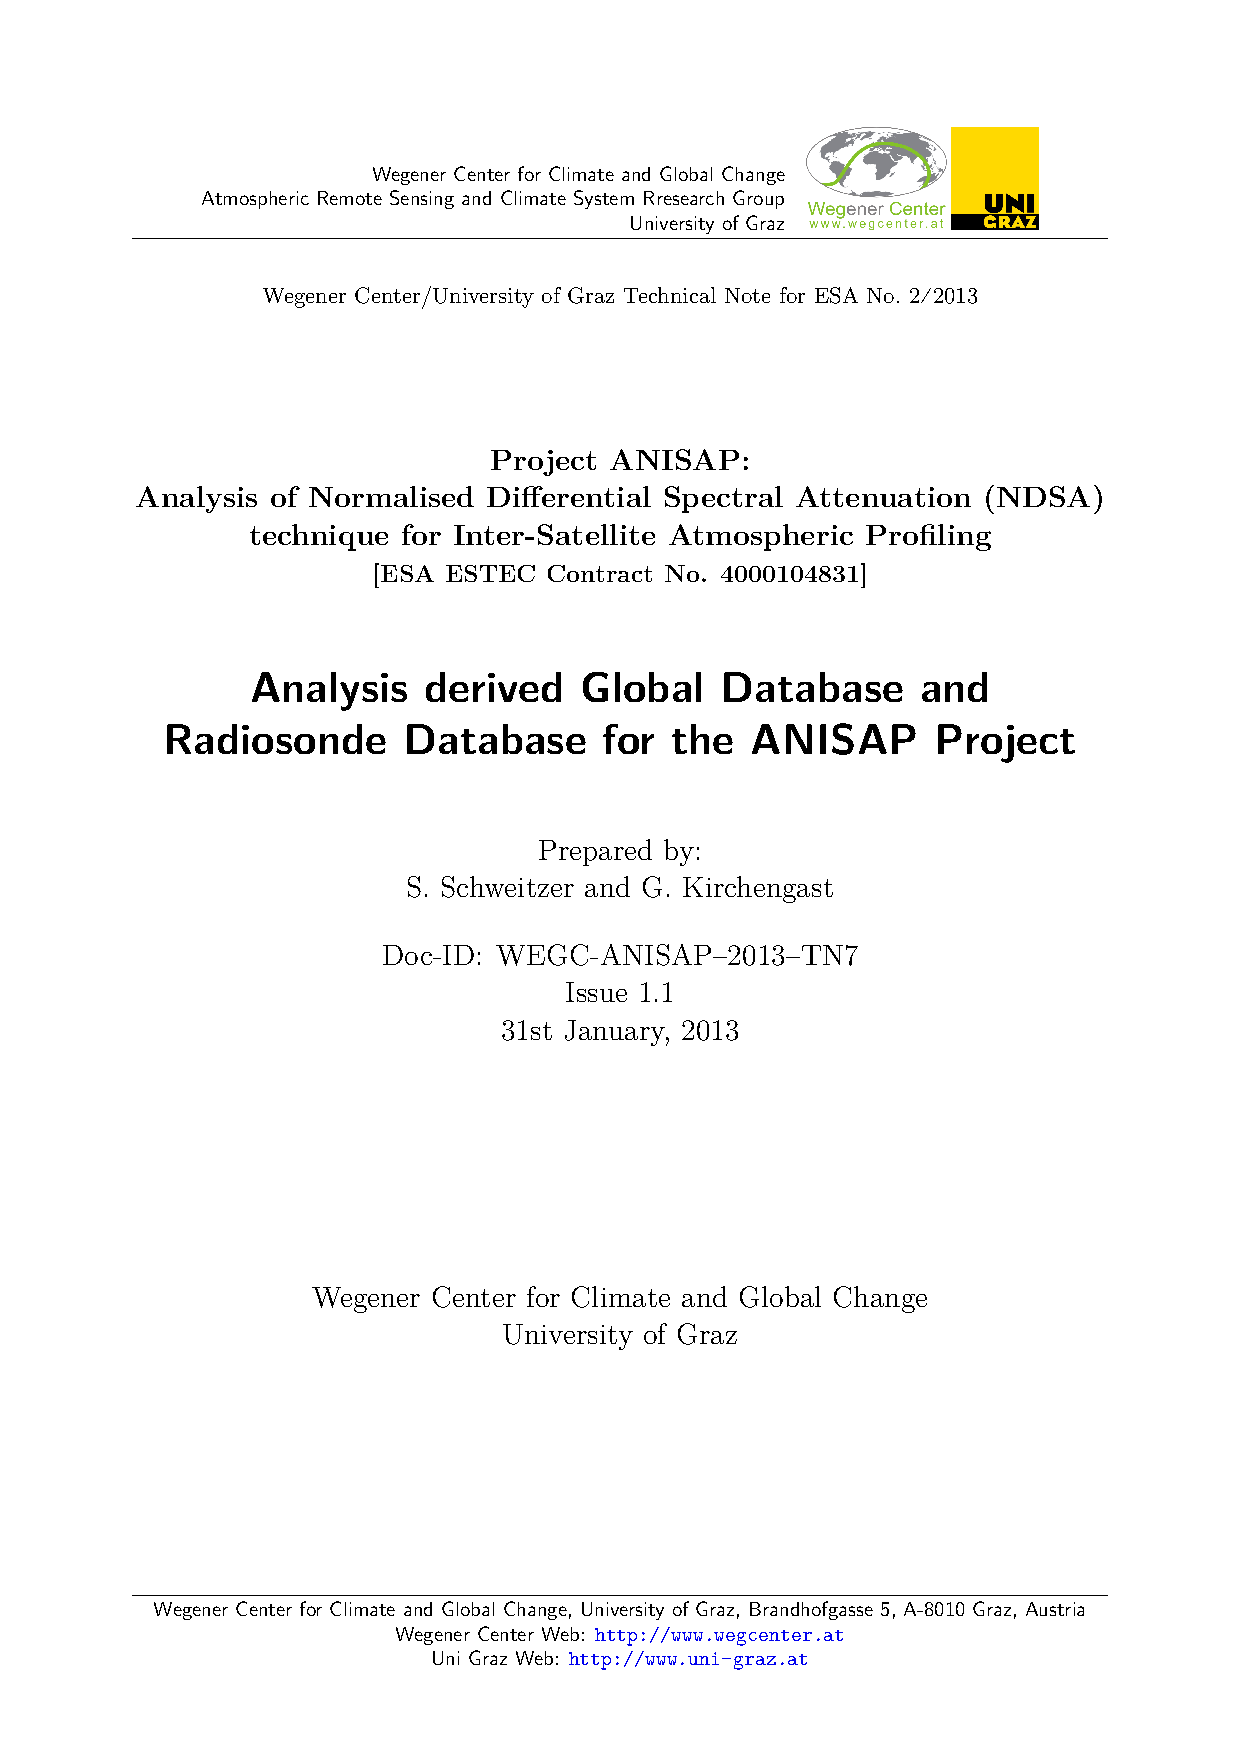
\includegraphics[height=0.7\paperheight, page=1]{anisap-TN2.pdf}}
  \caption{Example of a \multidoc document title page}
  \label{fig:multiDocTitlepage}
\end{figure}

\begin{figure}
  \centering
  \fbox{\includegraphics[height=0.7\paperheight, page=2]{anisap-TN2.pdf}}
  \caption{Example of a \multidoc document release information page}
  \label{fig:multiDocReleaseInfopage}
\end{figure}

\begin{figure}
  \centering
  \fbox{\includegraphics[height=0.7\paperheight, page=3]{anisap-TN2.pdf}}
  \caption{Example of a \multidoc document distribution list page}
  \label{fig:multiDocDistributionList}
\end{figure}

\begin{figure}
  \centering
  \fbox{\includegraphics[height=0.7\paperheight, page=4]{anisap-TN2.pdf}}
  \caption{Example of a \multidoc document change record page}
  \label{fig:multiDocChangeRecord}
\end{figure}

\begin{figure}
  \centering
  \fbox{\includegraphics[height=0.7\paperheight, page=10]{anisap-TN2.pdf}}
  \caption{Example of a \multidoc document random page}
  \label{fig:multiDocHeadings}
\end{figure}



\subsubsection[Document headings]{Tailoring the document headings}
\label{subsubsec:multiDocumentHeadings}

The layout of the document headings (\IE{} the header for the running
pages, see \autoref{fig:multiDocHeadings}) is the same for article, book
and report documents and is structured into three parts:
\begin{enumerate}
\item a four line text block on the left side (the exact definition of the
  concatenation of the string components is given in
  \autoref{lst:docstyleDocumentHeadingsTextBlock}) comprising
  \begin{enumerate}
  \item the document header title (built as a concatenated string from the
    document header title substring \latexcmd{\ThisDocHeaderTitleSubstr}
    and the document subtitle string \latexcmd{\ThisDocSubtitle}
  \item the document identifier (build as a concatenated string from the
    document identifier substring \latexcmd{\ThisDocIdSubstr}, the document
    release year \latexcmd{\ThisDocYear}, the document type%
    \footnote{The acronyms used for the various document types need to be
      defined in the file \path{acronyms.sty}, see
      \fullautoref{subsec:UsingTheAcronymDatabase}.}
    \latexcmd{\ThisDocType} (\EG{} \acs{tr} (\acl{tr}) or \acs{ar}
    (\acl{ar})), and the document internal number
    \latexcmd{\ThisDocIntNum})
  \item the document version (build as a concatenated string from the
    document issue number \latexcmd{\ThisDocIssue} and the document
    revision number \latexcmd{\ThisDocRevision}), and
  \item the document release date
  \end {enumerate}
\item a central single text line indicating the respective current section
  or chapter number and section or chapter title, and
\item a graphics block (of corporate logos) on the right side.
\end{enumerate}

The details and the structure of the document headings are defined in the
file \path{docstyle.sty} near line 315 to 354 (see
\autoref{lst:docstyleDocumentHeadings}).

Since individual details for a specific document from a \multidoc
documentation task are different from document to document due to the
different document content, document type, document identifiers, document
issue, document revision, document release date \ETC{}, these details are
only predefined in the file \path{docstyle.sty}, and intended to be
specifically tailored in each individual document's masterfile.

In essence, a block of redefining \LaTeX{} commands has to be added
(between the two already present commands \latexcmd{\makeatletter} and
\latexcmd{\makeatother}) to the master file, similar to the example given
in \autoref{lst:documentHeadingsExample}.
%
\begin{CommandLineListing}[style=DefaultFileListing, print=true, xleftmargin=0pt, gobble=2, %
  caption={Definition of document headings in the masterfile}, %
  label=lst:documentHeadingsExample]
  \makeatletter

  \renewcommand*{\ThisDocType}{%
    tr%
  }
  \renewcommand*{\ThisDocExtNum}{%
    03%
  }
  \renewcommand*{\ThisDocIntNum}{%
    37%
  }
  \renewcommand*{\ThisDocIssue}{%
    1%
  }
  \renewcommand*{\ThisDocRevision}{%
    3%
  }
  \renewcommand*{\subtitlePrefix}{%
    %
  }
  \renewcommand*{\ThisDocSubtitle}{%
    WLG Quickstart Guide%
  }
  \renewcommand*{\ThisDocHeaderTitleSubstr}{%
    \wegcLaTeX{}%
  }
  \renewcommand*{\ThisDocIdSubstr}{%
    \aces{wegc}-WLG-QSG%
  }
  \newdate{ThisDocDate}{13}{8}{2025}
  \renewcommand*{\ThisDocDate}{%
    \displaydate{ThisDocDate}%
  }
  \renewcommand*{\ThisDocYear}{%
    %% \getdateyear{ThisDocDate}%
    2028%
  }

  \makeatother
\end{CommandLineListing}

\lstinputlisting[style=DefaultFileListing, print=true,
   firstnumber=212, firstline=212, stepnumber=1, lastline=236,
   emptylines=*0,
   breaklines=true,
  caption={Definition of the documents headings text block in \texttt{\lstname}},
  label=lst:docstyleDocumentHeadingsTextBlock]{docstyle.sty}

\begin{landscape}
\lstinputlisting[style=DefaultFileListing, print=true,
   firstnumber=315, firstline=315, stepnumber=1, lastline=354,
   emptylines=*0,
   breaklines=true,
  caption={Definition of the document headings in \texttt{\lstname}},
  label=lst:docstyleDocumentHeadings]{docstyle.sty}
\end{landscape}


\subsubsection[Title page common elements]{Tailoring the common elements of the title page}
\label{subsubsec:multiDocumentTitlePageCommons}

The layout of the document title page is the same for article, book and
report documents and contains elements, which are common and the same for
all documents of a documentation task, \IE{} the title page header, the
title page footer, the document publisher details, the title head and the
subject details, and those that are different due to the individual
document content, \EG{} the document title or the document authors.


\minisec{Title page header and footer}

The common elements title page header and title page footer are defined and
specified in the file \path{docstyle.sty} near lines 252 and 271 (see
\autoref{lst:docstyleTitlepageHeaderFooter}).

\lstinputlisting[style=DefaultFileListing, print=true,
   firstnumber=252, firstline=252, stepnumber=1, lastline=281,
   emptylines=*1,
  caption={Definition of title page header and footer details in \texttt{\lstname}},
  label=lst:docstyleTitlepageHeaderFooter]{docstyle.sty}

If, for example, the combined \ac{igam}/\ac{wegc} title page header and
footer shall be replaced with the plain \ac{wegc} title page header and
footer, then the corresponding section in file \path{docstyle.sty} is to
be modified as shown in
\autoref{lst:docstyleTitlepageHeaderFooterWegcOnly}.
%
\begin{CommandLineListing}[style=DefaultFileListing, print=true, xleftmargin=0pt, gobble=2, %
  caption={Alternate definition of title page header and footer in \latexcmd{docstyle.sty}}, %
  label=lst:docstyleTitlepageHeaderFooterWegcOnly]
  \newcommand*{\Head@@ThisDocTitlePage}{%
    \upshape%
    \begin{varwidth}[b][0pt]{\paperwidth}%
      \LaTeXraggedleft%
      \Name{wegc}\\%
      %% \Name{igam}\\%
      \Name{ug}%
    \end{varwidth}%
    \quad%
    \begin{varwidth}[b][0pt]{\paperwidth}%
      
\includegraphics[height=50.0pt]{logo-ug-medium}%
      \hspace{2.0pt}%
      
\includegraphics[height=50.0pt]{logo-wegc-medium}%
      %% \hspace{2.0pt}%
      %% 
\includegraphics[height=50.0pt]{logo-igam-medium}%
    \end{varwidth}%
  }

  \newcommand*{\Foot@@ThisDocTitlePage}{%
    \upshape%
    \begin{varwidth}[t][0pt]{\paperwidth}%
      \LaTeXcentering%
      \Address{wegc}\\%
      %% \Address{igam}\\%
      \ShortName{wegc} Web\p: \WebAddress{wegc}\\%
      %% \ShortName{igam} Web\p: \WebAddress{igam}\\%
      \ShortName{ug} Web\p: \WebAddress{ug}\\%
    \end{varwidth}%
  }
\end{CommandLineListing}


\minisec{Title head and title subject details}

The title head and title subject details for the title page are defined in
the file \path{docstyle.sty} near lines 444 to 471 (see
\autoref{lst:docstyleTitlepageTitleheadSubject}).

\lstinputlisting[style=DefaultFileListing, print=true,
   firstnumber=444, firstline=444, stepnumber=1, lastline=471,
   emptylines=*0,
   caption={Definition of the title page title head and subject details in \texttt{\lstname}},
   label=lst:docstyleTitlepageTitleheadSubject]{docstyle.sty}

For changing the title page title head and subject details to something
different, the corresponding section in file \path{docstyle.sty} could
be modified as shown in
\autoref{lst:docstyleTitlepageTitleheadSubjectExample}.
%
\begin{CommandLineListing}[style=DefaultFileListing, print=true, xleftmargin=0pt, gobble=2, %
  caption={Alternate definition of title page title head and subject details in \latexcmd{docstyle.sty}}, %
  label=lst:docstyleTitlepageTitleheadSubjectExample]
  \newcommand*{\titleheadSubstr}{%
    \aces{wegc}%
  }
  \newcommand*{\titleheadSubSubstr}{%
    \aces{esa}%
  }
  \titlehead{%
    \makebox[\linewidth]{\titleheadSubstr \hbox{} \acel{\ThisDocType} for \titleheadSubSubstr \hbox{} \No{} \ThisDocExtNum\textfractionsolidus\ThisDocYear}%
  }
  \newcommand*{\subjectStr}{%
    rOPS Project\p:\\%
  }
  \newcommand*{\subjectSubstr}{%
    Typesetting and Document Generation%
  }
  \subject{%
    \subjectStr\subjectSubstr%
  }
\end{CommandLineListing}


\minisec{Publisher information}

The document publisher information for the title page is defined in the
file \path{docstyle.sty} near lines 504 to 520 (see
\autoref{lst:docstyleTitlepagePublisher}).

\lstinputlisting[style=DefaultFileListing, print=true,
   firstnumber=504, firstline=504, stepnumber=1, lastline=520,
   emptylines=*0,
   caption={Definition of the title page publisher details in \texttt{\lstname}},
   label=lst:docstyleTitlepagePublisher]{docstyle.sty}

For changing the title page publisher details to the plain \ac{wegc}
title page publisher details, the corresponding section in file
\path{docstyle.sty} is to be modified as shown in
\autoref{lst:docstyleTitlepagePublisherWegcOnly}.
%
\begin{CommandLineListing}[style=DefaultFileListing, print=true, xleftmargin=0pt, gobble=2, %
  caption={Alternate definition of title publisher details in \latexcmd{docstyle.sty}}, %
  label=lst:docstyleTitlepagePublisherWegcOnly]
  \newcommand*{\publishersSubstr}{%
    \acl{wegc}%
  }
  \newcommand*{\publishersSubSubstr}{%
    \acl{ug}%
  }
  \newcommand*{\publishersSubSubSubstr}{%
    %
  }
  \publishers{%
    \publishersSubstr\\\publishersSubSubstr\\\publishersSubSubSubstr%
  }
\end{CommandLineListing}


\minisec{Glossary and bibliography preambles}

If the default text for the preamble to the \emph{acronyms} and
\emph{abbreviations}, to the \emph{terms} and \emph{definitions}, or to the
bibliography does not fit as expected, these preambles can be modified in
\path{docstyle.sty}, starting near line 657 (see
\autoref{lst:docstyleGlossaryPreambles}) and near line 683 (see
\autoref{lst:docstyleBibliographyPreambles}).

\lstinputlisting[style=DefaultFileListing, print=true,
   firstnumber=657, firstline=657, stepnumber=1, lastline=670,
   emptylines=*0,
   caption={Definition of the glossary preambles in \texttt{\lstname}},
   label=lst:docstyleGlossaryPreambles]{docstyle.sty}

\lstinputlisting[style=DefaultFileListing, print=true,
   firstnumber=683, firstline=683, stepnumber=1, lastline=696,
   emptylines=*0,
   caption={Definition of the bibliography preambles in \texttt{\lstname}},
   label=lst:docstyleBibliographyPreambles]{docstyle.sty}


\subsubsection[Title page specific elements]{Tailoring the document specific elements of the title page}
\label{subsubsec:multiDocumentTitlePageSpecifics}

The layout of the document specific elements document title and authors are
predefined in the file \path{docstyle.sty} and need to be updated in each
individual document's masterfile by a block of redefining \LaTeX{} commands
which are to be added between the two already present commands
\latexcmd{\makeatletter} and \latexcmd{\makeatother}, similar to the
example given in \autoref{lst:documenTitlepageTitleExample}.

All other document specific elements required for the title page like
document type, document identifiers, document issue, document revision,
document release date \ETC{}, have already been described for the document
headings in \autoref{subsubsec:multiDocumentHeadings}

\Attention{%
  In \autoref{lst:documenTitlepageTitleExample}, the definition of the
  document subtitle is not explicitly shown, as it is already presented in
  \autoref{lst:documentHeadingsExample} of
  \autoref{subsubsec:multiDocumentHeadings} (due to the fact that
  \latexcmd{\subtitlePrefix} and \latexcmd{\ThisDocSubtitle} are used for
  the definition of the document headings).}

\begin{CommandLineListing}[style=DefaultFileListing, print=true, xleftmargin=0pt, gobble=2, %
  caption={Definition of document title and author details in the masterfile}, %
  label=lst:documenTitlepageTitleExample]
  \makeatletter
  ...
  ...
  \renewcommand*{\ThisDocTitle}{%
    The \wegcLaTeX{} documentation framework: \newline a guide for beginners%
  }
  \renewcommand*{\titlePrefix}{%
    %
  }
  \renewcommand*{\ThisDocAuthors}{%
    \ShortName{kmf}, \ShortName{jfb}, and \ShortName{gki}%
  }
  \makeatother
\end{CommandLineListing}


\subsubsection[A \multidoc document article]{Creating a \multidoc document article}
\label{subsubsec:creatingMultiDocumentArticle}

For creating a \multidoc article, proceed as follows:
%%
\begin{enumerate}
\item create a working directory for building the \wegcLaTeX{} \multidoc article, \\
  \EG{} \path{/home/\plh{user}/wlMultiDocTest/}

\item create the following subdirectories \\
  \path{/home/\plh{user}/wlMultiDocTest/wlg/}, \\
  \path{/home/\plh{user}/wlMultiDocTest/wlg/figs/}, \\
  \path{/home/\plh{user}/wlMultiDocTest/wlg/data/}, \\
  \path{/home/\plh{user}/wlMultiDocTest/wlg/tex/}, \\
  \path{/home/\plh{user}/wlMultiDocTest/common/}, and \\
  \path{/home/\plh{user}/wlMultiDocTest/common/figs}

  \Attention{Any further documents of a \multidoc documentation task would
    require the additional subdirectories \\
    \path{/home/\plh{user}/wlMultiDocTest/wlg2/}, \\
    \path{/home/\plh{user}/wlMultiDocTest/wlg2/figs/}, \\
    \path{/home/\plh{user}/wlMultiDocTest/wlg2/data/}, \\
    \path{/home/\plh{user}/wlMultiDocTest/wlg2/tex/}, \\
    and so on.}

\item copy the \LaTeX{} template master file \\
  \path{./texmf/doc/latex/wegc-latex/examples/multidoc-article/doc-article.tex} to \\
  \path{/home/\plh{user}/wlMultiDocTest/wlg/}

\item copy the seven \LaTeX{} source code files from \\
  \path{./texmf/doc/latex/wegc-latex/WLG/} to \\
  \path{/home/\plh{user}/wlMultiDocTest/wlg/tex/}

\item copy the twelve \path{*.png} and twelve \path{*.xbb} files from \\
  \path{./texmf/doc/latex/wegc-latex/examples/common/figs/} to \\
  \path{/home/\plh{user}/wlMultiDocTest/common/figs/}

\item copy the three files
  \path{docstyle.sty}, \path{project.sty}, and \path{commands.sty} from \\
  \path{./texmf/doc/latex/wegc-latex/examples/common/} to \\
  \path{/home/\plh{user}/wlMultiDocTest/common}

 \item extract the three example only files \path{acronyms.sty}, \path{addresses.sty}, and
  \path{terms.sty} from the compressed archive file \\
  \path{./texmf/doc/latex/wegc-latex/WLG/acronymsAddressesTerms_ExampleDoNotUse.tar.gz}
  or use the current and up to date versions available at 
  \nolinkurl{https://wegc203117.uni-graz.at/projects/latex_dbs/browser/arsclisys}
  and put them to \\
  \path{/home/\plh{user}/wlMultiDocTest/common}

\item add the address for the fictive person ``\Name{kmf}'' at the end of
  the copied file \path{addresses.sty}, as described in
  \autoref{subsec:usingTheAddressBookDatabase}

\item add the acronym for the fictive company ``\acf{tmc}'' at the end of
  the copied file \path{acronyms.sty}, as described in
  \autoref{subsec:UsingTheAcronymDatabase}

\item add the glossary entry for the fictive term ``\Gls{firlefanzation}''
  at the end of the copied file \path{terms.sty}, as described in
  \autoref{subsec:UsingTheGlossaryDatabase}

\item create an example bibliography file \path{exampleBibFile.bib} in the \\
  \path{/home/\plh{user}/wlMultiDocTest/wlg} directory in the same way as
  it is described for a \singledoc article (see
  \autoref{subsubsec:creatingSingleDocumentArticle})

\item copy the template master file \\
  \path{/home/\plh{user}/wlMultiDocTest/wlg/doc-wlarticle.tex} to \\
  \path{/home/\plh{user}/wlMultiDocTest/wlg/md-wlgArticle.tex} \\
  and apply the following modifications:
  \begin{enumerate}
  \item at line 119, change \latexcmd{DIV=default} to \latexcmd{DIV=11}
  \item between the lines 165 to 171, reading
    \begin{CommandLineListing}[style=DefaultFileListing, print=true, basicstyle={\ttfamily\small}, %
      basewidth=0.47em, xleftmargin=0pt, gobble=6]
      \makeatletter
      %% NOTE: Here, we can act as class and package authors if we want or need to do so ...
      \makeatother
    \end{CommandLineListing}
    add the definition commands for defining the document specific settings:
    \begin{CommandLineListing}[style=DefaultFileListing, print=true, basicstyle={\ttfamily\small}, %
      basewidth=0.47em, xleftmargin=0pt, gobble=6]
      \makeatletter

      \renewcommand*{\ThisDocType}{%
        tr%
      }
      \renewcommand*{\ThisDocExtNum}{%
        03%
      }
      \renewcommand*{\ThisDocIntNum}{%
        37%
      }
      \renewcommand*{\ThisDocIssue}{%
        1%
      }
      \renewcommand*{\ThisDocRevision}{%
        3%
      }
      \renewcommand*{\subtitlePrefix}{%
        %
      }
      \renewcommand*{\ThisDocSubtitle}{%
        WLG Quickstart Guide%
      }
      \renewcommand*{\ThisDocHeaderTitleSubstr}{%
        \wegcLaTeX{}%
      }
      \renewcommand*{\ThisDocIdSubstr}{%
        \aces{wegc}-WLG-QSG%
      }
      \newdate{ThisDocDate}{13}{8}{2025}
      \renewcommand*{\ThisDocDate}{%
        \displaydate{ThisDocDate}%
      }
      \renewcommand*{\ThisDocYear}{%
        %% \getdateyear{ThisDocDate}%
        2028%
      }
      \renewcommand*{\ThisDocTitle}{%
        The \wegcLaTeX{} documentation framework: \newline a guide for beginners%
      }
      \renewcommand*{\titlePrefix}{%
        %
      }
      \renewcommand*{\ThisDocAuthors}{%
        \ShortName{kmf}, \ShortName{jfb}, and \ShortName{gki}%
      }
      \makeatother
    \end{CommandLineListing}

  \item on lines 150 to 151: change from
    \begin{CommandLineListing}[style=DefaultFileListing, print=true, basicstyle={\ttfamily\small}, %
      basewidth=0.47em, xleftmargin=0pt, gobble=6]
      \bibliography{%
      }
    \end{CommandLineListing}
    to
    \begin{CommandLineListing}[style=DefaultFileListing, print=true, basicstyle={\ttfamily\small}, %
      basewidth=0.47em, xleftmargin=0pt, gobble=6]
      \bibliography{%
        exampleBibFile%
      }
    \end{CommandLineListing}

  \item between lines 165 and 171, reading
    \begin{CommandLineListing}[style=DefaultFileListing, print=true, basicstyle={\ttfamily\small}, %
      basewidth=0.47em, xleftmargin=0pt, gobble=6]
      \makeatletter

      %% NOTE: Here, we can act as class and package authors if we want or need to do so ...

      \makeatother
    \end{CommandLineListing}
    add the following command definitiosn for \entity{singledoc} and \entity{multidoc}:
    \begin{CommandLineListing}[style=DefaultFileListing, print=true, basicstyle={\ttfamily\small}, %
      basewidth=0.47em, xleftmargin=0pt, gobble=6]
      \makeatletter

      %% NOTE: Here, we can act as class and package authors if we want or need to do so ...

      \newcommand*{\singledoc}{%
        \entity{singledoc} %
      }

      \newcommand*{\multidoc}{%
        \entity{multidoc} %
      }

      \makeatother
    \end{CommandLineListing}

  \item \label{item:nociteGlsaddIncludeDirectives} between the lines 201
    and 204, reading
    \begin{CommandLineListing}[style=DefaultFileListing, print=true, basicstyle={\ttfamily\small}, %
      basewidth=0.47em, xleftmargin=0pt, gobble=6]
      \printbibliography[prenote=refpreamble]


      \appendix
    \end{CommandLineListing}
    add the following content:
    \begin{CommandLineListing}[style=DefaultFileListing, print=true, basicstyle={\ttfamily\small}, %
      basewidth=0.47em, xleftmargin=0pt, gobble=6]
      \printbibliography[prenote=refpreamble]

      \nocite{Gorbunov2007a}
      \nocite{Gorbunov2002a}
      \nocite{Gorbunov1986}

      \glsadd{development_team}
      \glsadd{firlefanzation}

      \glsadd{urd}
      \glsadd{add}
      \glsadd{ddd}
      \glsadd{sum}
      \glsadd{atr}

      
\section[Introduction]{Introduction}
\label{sec:introduction}



\subsection[Scope]{Scope}
\label{subsec:scope}

The intention of this document\footnote{The document in hand is applicable
  to \software{long}{\wegcLaTeX}{0}{9}{5}{200}\p.} is to give new users of
the \wegcLaTeX{} documentation framework a quick introduction on how to use
it in the most efficient way.

Included in this manual are a series of examples on how to create the document layout and how to
use the capabilities of the automatically included \LaTeX{} packages.
No special treatment for typesetting formulas, diagrams or tables is given, as literature
on these topics is readily available.
To a minor extent, it also covers advanced topics mainly relevant to people who want to use \wegcLaTeX{}
within the scope of documentation tasks.

It must be emphasized that it is far beyond the scope of this user guide to address questions about
standard \LaTeX{} concepts. Using \LaTeX{} in a reasonably correct manner is \emph{not} a trivial task.
In fact, it is easy to use it quite wrongly.
It is expected that the reader has a basic understanding on how to create simple \LaTeX{} documents.
So if you are new to \LaTeX{} and/or have never worked in a \LaTeX{} documentation task,
please refer to introductory literature on \LaTeX{}.

At the minimum, you should read %
\textquote[\ctanurl{/tex-archive/info/lshort/english/lshort.pdf}]{%
  The Not So Short Introduction to \LaTeXe%
} %
which provides a very good survey of contemporary \LaTeX{} for both beginners and advanced users.
Nevertheless, it is recommended to study the following documents in some detail:
%
\begin{itemize}
   \item \textquote[]{\LaTeXe{} for authors}
         \footnote{\ctanurl{/tex-archive/macros/latex/doc/usrguide.pdf}}

   \item \textquote[]{An essential guide to \LaTeXe{} usage}
         \footnote{\ctanurl{/tex-archive/info/l2tabu/english/l2tabuen.pdf}}

   \item \textquote[]{\KOMAScript}
         \footnote{\ctanurl{/tex-archive/macros/latex/contrib/koma-script/doc/scrguide.pdf}}

   \item \textquote[]{Math mode}
         \footnote{\url{ftp://ftp.tex.ac.uk/tex-archive/info/math/voss/mathmode/Mathmode.pdf}}

   \item \textquote[]{Using Imported Graphics in \LaTeX{} and pdf\LaTeX}
         \footnote{\ctanurl{/tex-archive/info/epslatex/english/epslatex.pdf}}
\end{itemize}
%
Finally, download and print out the %
\textquote[\url{http://www.stdout.org/~winston/latex/latexsheet.pdf}]{%
  \LaTeXe{} Cheat Sheet%
} %
since this may serve as a handy means for everyday work with \LaTeX.

\wegcLaTeX{} has been developed and is maintained by \Name{mip}. In case of
any questions about \wegcLaTeX{}, please write an email to
\EmailAddress{mip}.



\subsection{Capabilities of \wegcLaTeX{}}
\label{subsec:capabilities}

So, what is the \wegcLaTeX{} documentation framework?
Stated in the most simple way, \wegcLaTeX{} provides an environment for generating documents with a
consistent look and feel. The consistency of the the documents is ensured by providing mechanisms
for consistent usage of common items like names, addresses, email addresses, web addresses, telephone numbers,
abbreviations, acronyms, terms and last but not least, a common and consistent document style for
\singledoc and \multidoc documents.

\smallskip

\singledoc documents have a traditional \LaTeX{} styling, whereas \multidoc
documents are intended for publications that comprise two or more articles,
reports or books, which shall all share a common and consistent layout of
the document front matter, \EG{} title page, distribution list and document
revision history as well as document headings. For a few sample pages of a
\multidoc document, please see \autoref{fig:multiDocTitlepage},
\autoref{fig:multiDocReleaseInfopage},
\autoref{fig:multiDocDistributionList}, \autoref{fig:multiDocChangeRecord}
and \autoref{fig:multiDocHeadings} in
\fullautoref{subsec:usingMultiDocumentTemplates}.

The documents written with \wegcLaTeX{} can be, for example, the
documentation tree associated with a software package, the manual and
handbook set for operating and maintenance procedures of any type of machinery, 
or single documents like \ac{msc} and \ac{phd} theses 
(please see \fullautoref{subsubsec:creatingMasterOrPhdThesis} for an expample),
scientific or technical reports, or papers.

\wegcLaTeX{} provides the means to ensure the consistent layout of the
documents by providing templates for the layout of front matter pages,
title page, distribution list, document revision history, bibliography, as
well as of the lists of figures and tables.

Due to the fact that \wegcLaTeX{} also automatically imports a series of
handy \LaTeX{} packages for the creation and inclusion of external
pictures, diagrams, verbatim text and pretty-printed source code listings,
the user does not need to load any extra packages, but can simply start
writing his or her documentation, taking the provided example documents as
a starting point.

As its name implies, \wegcLaTeX{} is written in the \LaTeX{} document
markup language which is widely used by scientists and other professionals
in both the academic and commercial world.  Distributed under the terms of
the \ac{lppl}, \LaTeX{} is free software.%
\footnote{%
  This statement has sometimes been questioned (\CF{}
  \url{http://en.wikipedia.org/wiki/LPPL}).%
} %
Owing to its platform independence, it can moreover be used in a similar
way on Linux, \ac{mac_os_x}, and Windows machines.

Contemporary \TeX/\LaTeX{} distributions such as \TeXLive{} and \MiKTeX{}
ship with a considerable variety of modules whose capabilities go far
beyond the potentials originally foreseen by the venerable \TeX{}
typesetting system and the \LaTeX{} kernel built on it. In fact, assuming
you are an experienced and sufficiently persistent \LaTeX{} user, you
should nowadays be able to cope with most tasks that might arise while
preparing scientific and/or technical documents.  An incomplete---and, of
course, subjective---list of modules providing the necessary tools for
doing so includes:
%
\begin{labeling}[→]{\KOMAScript{} bundle}
   \item[\KOMAScript{} bundle]%
      modern and highly configurable replacement for the standard \LaTeX{}
      document classes, sophisticated interface for configuring the document
      layout including page style design%
      \footnote{\ctanurl{/tex-archive/macros/latex/contrib/koma-script/doc/scrguide.pdf}}
   \item[\entity{babel} package]%
      multilingual support%
      \footnote{\ctanurl{/tex-archive/macros/latex/required/babel/base/babel.pdf}}
   \item[\entity{url} package]%
      formatting \acp{url}, email addresses, filenames, etc.%
      \footnote{\ctanurl{/tex-archive/macros/latex/contrib/url/url.pdf}}
   \item[\entity{siunitx} package]%
      formatting units of physical quantities%
      \footnote{\ctanurl{/tex-archive/macros/latex/contrib/siunitx/siunitx.pdf}}
   \item[\entity{amsmath} package]%
      high‐quality typesetting of mathematical formulae%
      \footnote{\ctanurl{/tex-archive/macros/latex/required/amslatex/math/amsldoc.pdf}}
   \item[\entity{array} package]%
      replacement for the standard \LaTeX{} tables and arrays%
      \footnote{\ctanurl{/tex-archive/macros/latex/required/tools/array.pdf}}
   \item[\entity{booktabs} package]%
      assistance in producing publication‐quality tables%
      \footnote{\ctanurl{/tex-archive/macros/latex/contrib/booktabs/booktabs.pdf}}
   \item[\entity{longtable} package]%
      creating multipage tables%
      \footnote{\ctanurl{/tex-archive/macros/latex/required/tools/longtable.pdf}}
   \item[\entity{xcolor} package]%
      colour support%
      \footnote{\ctanurl{/tex-archive/macros/latex/contrib/xcolor/xcolor.pdf}}
   \item[\entity{graphicx} package]%
      embedding external graphics given in various formats%
      \footnote{\ctanurl{/tex-archive/macros/latex/required/graphics/grfguide.pdf}}
   \item[\entity{pgf} package]%
      creating graphics%
      \footnote{\ctanurl{/tex-archive/graphics/pgf/base/doc/generic/pgf/pgfmanual.pdf}}
   \item[\entity{mhchem} package]%
      chemical formulae%
      \footnote{\ctanurl{/tex-archive/macros/latex/contrib/mhchem/mhchem.pdf}}
   \item[\entity{listings} package]%
      pretty-printing of source code%
      \footnote{\ctanurl{/tex-archive/macros/latex/contrib/listings/listings.pdf}}
   \item[\entity{glossaries} package]%
      maintaining glossaries, lists of acronyms, indices, etc.\ with
      assistance of the \path{makeindex} program%
      \footnote{\ctanurl{/tex-archive/macros/latex/contrib/glossaries/glossaries-user.pdf}}
   \item[\entity{biblatex} package]%
      maintaining bibliographies based on \BibTeX{} bibliographic database
      files with assistance of the \path{bibtex8} program%
      \footnote{\label{fnote:biblatex}\ctanurl{/tex-archive/macros/latex/exptl/biblatex/doc/biblatex.pdf}}
   \item[\entity{hyperref} package]%
      support for hyperlinks, \ac{pdf} bookmarks, \ac{pdf} document
      information, etc.%
      \footnote{\ctanurl{/tex-archive/macros/latex/contrib/hyperref/doc/manual.pdf}}
   \item[\entity{pdfpages} package]%
      support for inclusion of excerpts from \ac{pdf} documents, etc.%
      \footnote{\ctanurl{/tex-archive/macros/latex/contrib/pdfpages/pdfpages.pdf}}
\end{labeling}


Since 2008, \wegcLaTeX{}, a general purpose document preparation
framework, selects, configures, patches, and extends an adequate
subset of \LaTeX{} modules available from \ac{ctan} according to the
needs of a typical user with scientific and/or technical
background. Not surprisingly, the basis of \wegcLaTeX{} is formed by
just those modules outlined in the preceding list.\footnote{Links to
  the documentation of further \LaTeX{} packages used in \wegcLaTeX{}
  are provided with the corresponding \latexcmd{\RequirePackage{}}
  statements in the \path{wltools.sty} and \path{wlsetup.sty} style
  files of the \wegcLaTeX{} framework} To sum up once more, it can be
said that \wegcLaTeX{} represents a highlevel interface to \LaTeX{}
which should enable its user to write comprehensible, consistent,
reader-friendly, flexible, and easily maintainable scientific and/or
technical documents without being forced to spend much time on looking
into more than the (already comprehensive) fundamentals of the
\LaTeX{} document markup language.

      

\section{Installation}
\label{sec:installation}


\subsection{Installation instructions}
\label{sec:installationInstructions}

\wegcLaTeX{} is provided in the repository hosted at
\nolinkurl{svn+ssh://wegc203117.uni-graz.at/var/lib/svn/wegc_latex/}.

The prerequisite for using \wegcLaTeX{} is a properly installed full \TeXLive{} 2012 distribution on a Linux workstation,
\IE{} the following packages:
\begin{description}
   % \item for \entity{SuSE 12.2}: \\
   %    \path{texlive}, \path{texlive-latex}, \path{texlive-bin-latex}, \\
   %    \path{texlive-tools}, \path{texlive-bin-tools}, \path{texlive-doc}, and \path{texlive-fonts-extra}
   \item for \entity{Debian 7}: \\
      \path{texlive}, and \path{texlive-full}
\end{description}

It should be noted at this place that \wegcLaTeX{} has not been tested with
\MiKTeX{} yet. Experience shows, however, that, if any, only minor
compatibility issues are to be expected.

For installing \wegcLaTeX{} it is only necessary to copy the \wegcLaTeX{}
\texmf{} tree to the \path{\plh{InstallDir}/texmf} directory, and to set up
to three environment variables. \path{\plh{InstallDir}} denotes the
directory in which \path{./texmf/} itself resides, \EG{} if the user's home
directory is used, to \path{/home/<userId>/texmf/}.

Assuming a workstation using the \entity{bash} command language
interpreter, as a second and final step, setting the three environment
variables can be done by adding the following three lines to the
\path{.bashrc} login script:
%
\begin{CommandLineListing}[style=DefaultFileListing, print=true, gobble=3]
   export TEXMFHOME=<InstallDir>/texmf
   export TEXINPUTS=.:./\{data,figs,tex\}//:../common//:
   export BIBINPUTS=.:../common//:
\end{CommandLineListing}
%
\begin{itemize}
\item The \cmdline{TEXMFHOME} variable defines the \wegcLaTeX{}
  installation directory. In this example, it is set to
  \cmdline{TEXMFHOME=<InstallDir>/texmf}. This is only necessary if
  \wegcLaTeX{} is installed to a directory other than the user's home
  (\path{/home/<userId>/}) or the system's pre-defined path
  (\path{/usr/local/share/}). The \LaTeX{} interpreter searches these two
  paths automatically and will use \wegcLaTeX{}, if found there, also
  without setting the \cmdline{TEXMFHOME} variable.
\item The \cmdline{TEXINPUTS} variable defines the locations where
  \wegcLaTeX{} searches for required packages, data, figures, or \LaTeX{}
  source code files. This is convenient, since any file in the
  \path{./data/}, \path{./figs/}, \path{./tex/} or \path{./common/}
  subdirectories can then be referred to by its basename instead of its
  (absolute or relative) pathname.
\item The \cmdline{BIBINPUTS} variable defines the locations where
  \wegcLaTeX{} searches for \path{*.bib} files.
\end{itemize}
%
\Attention{%
  You should not forget to replace the example directory names with the
  real directory names of your installation. Moreover, you must
  \enquote{source} your \path{~/.bashrc} (\IE{} by entering \cmdline{source
    ~/.bashrc} on the command line) in order for the modified shell
  environment to come into effect. If you already maintain a personal
  \texmf{} tree in a non‐standard location, say \path{~/pubs/texmf}, ensure
  that the above two commands are interpreted \emph{after} the commands
  setting up the shell environment for your personal \texmf{}
  tree. Otherwise, there is some probability that \wegcLaTeX{} will not get
  what it actually expects \ldots
}


\subsection{\wegcLaTeX{} file structure}
\label{subsec:structure}

All files belonging to the \wegcLaTeX{} framework are stored below the
\path{\plh{InstallDir}/texmf/} directory. \path{\plh{InstallDir}} denotes
the directory in which the \path{./texmf/} itself resides.
%
The file structure follows the concept of a so‐called \texmf{} tree. At first
glance, you might deem this structure unnecessarily complicated. As a
matter of fact, it is, however, most adequate, given that the file search
algorithms included in \TeX⁄\LaTeX{} distributions such as \TeXLive{} and
\MiKTeX{} are definitely designed and optimized for \texmf{} trees.

The subsequent list describes the subdirectories of the \wegcLaTeX{} file structure:
\begin{description}
   \item \path{./texmf/bibtex/} \\
      This directory hosts \entity{biblatex}-related files (\EG, style files).
    \item \path{./texmf/doc/} \\
      This directory contains the \wegcLaTeX{} templates for
      \singledoc and \multidoc documents in the \\
      \path{./texmf/doc/latex/wegc-latex/examples/singledoc/}, \\
      \path{./texmf/doc/latex/wegc-latex/examples/multidoc-article/}, \\
      \path{./texmf/doc/latex/wegc-latex/examples/multidoc-report/}, and \\
      \path{./texmf/doc/latex/wegc-latex/examples/multidoc-book/} \\
      directories, as well as the document command and layout template files in the \\
      \path{./texmf/doc/latex/wegc-latex/examples/common/} directory.
   \item \path{./texmf/doc/latex/wegc-latex/examples/singledoc/} \\
      This directory contains the \singledoc article, report and book document templates, \IE,
      \path{master-wlarticle.tex}, \path{master-wlreport.tex}, and \path{master-wlbook.tex}.
   \item \path{./texmf/doc/latex/wegc-latex/examples/multidoc-article/}, \\
         \path{./texmf/doc/latex/wegc-latex/examples/multidoc-report/}, and \\
          \path{./texmf/doc/latex/wegc-latex/examples/multidoc-book/} \\
      These directories contain \multidoc article, report and book document templates, \IE, \\
      \path{./multidoc-article/doc-article.tex}, \\
      \path{./multidoc-book/doc-book.tex}, and \\
      \path{./multidoc-report/doc-report.tex}. \\
      Each of these three subdirectories also contain a
      \path{./data/},
      \path{./figs/} and
      \path{./tex/} subdirectory for storing ASCII, image and \LaTeX{} files used.
   \item \path{./texmf/doc/latex/wegc-latex/examples/common/} \\
      This directory contains the \singledoc and \multidoc document command and layout template files \\
      \path{./common/commands.sty}, \\      
      \path{./common/docstyle.sty}, and \\
      \path{./common/project.sty}. \\
      The acronyms, terms, and address definition files 
      \path{acronyms.sty},
      \path{addresses.sty}, and
      \path{terms.sty} are also to be put into this directory 
      (example only versions of these files are provided in the compressed archive file
      \path{./texmf/doc/latex/wegc-latex/WLG/acronymsAddressesTerms_ExampleDoNotUse.tar.gz}, 
      whereas current and up to date versions of these files should be obtained from the separate 
      repository hosted at
      \nolinkurl{https://wegc203117.uni-graz.at/projects/latex_dbs/browser/arsclisys}.%%
      \footnote{The common acronyms, terms, and address
        definitions are easily accessed by adding its directory path to the
        \path{TEXINPUTS} environment variable.} \\
      %%
      The subdirectory \\
      \path{./common/figs/} \\
      contains the images used with \multidoc document cover pages and document headers.
   \item \path{./texmf/dvipdfmx/} \\
      This directory hosts configuration files for the \entity{DVIPDFMx} package,
      used for translating the \entity{DVI} format to \entity{PDF}.
   \item \path{./texmf/tex/} \\
      This directory hosts, among others, the automatically included \LaTeX{} modules mentioned previously
      and the \wegcLaTeX{} kernel.
   \item \path{./texmf/tex/<TBD>/documentVersionInfo.tex} \\
      This file contains the revision definitions used by \wegcLaTeX{}
      (intended to be updated by a \path{./configure} or \path{./makeDocument} script).
      The revision definition consists of three entities, \IE{} \\
      \cmdline{documentRevision},
      \cmdline{documentMajorVersion}, and
      \cmdline{documentMinorVersion}:
      %
      \begin{CommandLineListing}[print=true, gobble=6]
         \newcommand*{\documentMajorVersion}{5}
         \newcommand*{\documentMinorVersion}{6}
         \newcommand*{\documentRevision}{3072}
      \end{CommandLineListing}
\end{description}

For easier offline reading, the manuals for the \LaTeX{} packages mentioned
in \fullautoref{subsec:scope}, \fullautoref{subsec:capabilities} and
\fullautoref{subsec:extensionsToTheLatexKernel}, together with this manual
(\path{WLG.pdf}), are provided in the directory \path{./LaTeX_PDFs/} as
\ac{pdf} files (at the same directory level as the \wegcLaTeX{} \texmf{}
tree).



\subsection{Generating this document}
\label{subsec:generatingThisDocument}

Assuming the \wegcLaTeX{} framework is already properly installed (see \autoref{sec:installationInstructions}),
for generating this document, proceed as follows:
%%
\begin{enumerate}
   \item
      create a working directory, \EG{} \path{/home/\plh{user}/wlgDocGen/}
   \item
      checkout the latest version of \wegcLaTeX{} to \path{/home/\plh{user}/wlgDocGen/}
   \item
      change to the directory containing the master file \path{WLG.tex}, \IE{} \\
      \cmdline{cd /home/\plh{user}/wlgDocGen/trunk/texmf/doc/latex/wegc-latex/WLG}
   \item
      execute the script \path{makeWLG}, \IE{} \\
      \cmdline{./makeWLG} \\
      for generating the \entity{PDF} file \path{WLG.pdf}
\end{enumerate}

      
\section{Document generation}
\label{sec:documentGeneration}



\subsection{Commands for document generation}
\label{subsec:commandsForDocumentGeneration}

Assuming that a complete document has been properly written, all the required subdocument \LaTeX{} source code files, data and figure
files are present in the appropriate subdirectories (as described in \autoref{subsec:structure} on \autopageref{subsec:structure}),
and the master \LaTeX{} file is named \path{masterDoc.tex},
then there are 4 steps necessary for generating the print-ready \entity{PDF} document:

\begin{enumerate}

   \item
   \begin{enumerate}
      \item
         \label{item:pdf_mode}
         \cmdline{pdflatex masterDoc} \\
         Generate the output document in \entity{PDF} format by calling
         \pdfTeX{} in \entity{PDF} mode.  In this case,
         \latexcmd{\documentclass} should include the \cmdline{"pdftex"}
         output driver option. This is the recommended (and default) way.
      \item
         \label{item:dvi_mode}
         \cmdline{latex masterDoc && dvipdfmx masterDoc} \\
         Alternatively, generate the output document in \entity{PDF} format by calling either \TeX{} or \pdfTeX{} in \entity{DVI} mode.
         In this case, \latexcmd{\documentclass} should include the \cmdline{"dvipdfmx"} output driver option.
         If \pdfTeX{} is not installed this command replaces the preceding command.
         If \pdfTeX{} is installed it is an alternative to the preceding command, allowing to generate the output document in a way
         closer to how it would be generated by means of the traditional \TeX{} engine.
         Note that this may imply a significantly smaller \entity{PDF} file size.
   \end{enumerate}

   \item
      \label{item:glossaries}
      \cmdline{makeglossaries masterDoc} \\
      Generate \LaTeX{} code for formatting the glossary sections. Which
      index processor is internally called by the makeglossaries program
      depends on the value of the \cmdline{"glossaries/processor"}
      \latexcmd{\documentclass} option.  It can be \cmdline{"makeindex"} or
      \cmdline{"xindy"}. Default is \cmdline{"makeindex"}.

   \item
   \begin{enumerate}
      \item
         \label{item:bibliographyBT8}
         \cmdline{bibtex8 -c <csfile> -W masterDoc} \\
         Generate \LaTeX{} code for formatting the bibliography section by
         means of the \cmdline{bibtex8} program.  In this case,
         \latexcmd{\documentclass} should set the
         \cmdline{"biblatex/backend"} option to \cmdline{"bibtex8"} (this
         is the default). \cmdline{<csfile>} denotes a \BibTeX{} character
         set and sort definition file such as \path{ascii.csf},
         \path{latin1.csf} or \path{latin9.csf}.  This should match the
         encoding of the bibliographic database. Usually you do not need to
         explicitly set the \cmdline{<csfile>}, leaving you with the
         recommended way of formatting the bibliography:\\\cmdline{bibtex8
           -W masterDoc}.
      \item
         \label{item:bibliographyBT}
         \cmdline{bibtex masterDoc} \\
         Generate \LaTeX{} code for formatting the bibliography section by
         means of the bibtex program. In this case,
         \latexcmd{\documentclass} should set the
         \cmdline{"biblatex/backend"} option to \cmdline{"bibtex"}.
   \end{enumerate}

 \item Repeat \autoref{item:pdf_mode} or \autoref{item:dvi_mode} two more
   times to get all references and hyperlinks such as
   \latexcmd{\autoref{}}, \latexcmd{\ac{}} and/or \latexcmd{\textcite{}}
   \ETC{} properly updated.

\end{enumerate}

An example script, which uses as first argument the basename of the
\LaTeX{} master file, is presented in
\autoref{lst:documentGenerationScript}. Please note that during your daily
working routine, it is not necessary to perform all these steps; in most
cases, a simple run of \autoref{item:pdf_mode} will update your
\entity{PDF} most efficiently.

\Attention{%
  The more traditional \path{tex}→\path{dvi}→\path{pdf} document generation
  approach listed under \autoref{item:dvi_mode} does not work well at the
  moment because a few \LaTeX{} modules loaded by \wegcLaTeX{}
  insufficiently support the underlying \entity{dvipdfm} driver.
  Furthermore note that the \entity{glossaries} package does not give any
  indication whether \path{makeindex} must be called at a specific stage of
  document generation to update the \enquote{\glossaryname} and
  \enquote{\acronymname} sections as outlined under
  \autoref{item:glossaries}.  Unfortunately, this circumstance makes the
  implementation of an \emph{intelligent} build system a rather challenging
  task.  Assuming the \enquote{\bibname} section is very large and⁄or
  several secondary reference lists exist, calling \path{bibtex8} is likely
  to result in an error despite specifying the high‐capacity
  \path{-W} switch suggested under
  \autoref{item:bibliographyBT8}. If this happens, resort to the
  \entity{biblatex} package documentation (see \autoref{fnote:biblatex})
  which describes in detail how to maximize the capacity of the
  \path{bibtex8} program at run time.}


\begin{CommandLineListing}[style=DefaultFileListing, print=true, basicstyle={\ttfamily\small}, %
                           basewidth=0.47em, xleftmargin=0pt, gobble=3, %
                           caption={Example script for document generation}, %
                           label=lst:documentGenerationScript]
   #! /bin/bash
   export TEXMFHOME=/home/<userId>/texmf
   export TEXINPUTS=.:./\{data,figs,tex\}//:../common//:
   export BIBINPUTS=.:../common//:

   masterDoc=${1}
   latex=pdflatex
   makeglossaries=makeglossaries
   bibtex='bibtex8 -W'
   rm='/bin/rm -f'
   intermediateFiles='*.acn *.acr *.alg *.aux *.bbl *.blg *-blx.bib *.dvi *.glo *.glg *.gls *.ist *.lof *.log *.lol *.lot *.nlg *.noa *.not *.run.xml *.toc'
   ${rm} ${intermediateFiles} &&
   ${latex} ${masterDoc} &&
   ${makeglossaries} ${masterDoc} &&
   ${bibtex} ${masterDoc} &&
   ${latex} ${masterDoc} &&
   ${makeglossaries} ${masterDoc} &&
   ${latex} ${masterDoc} &&
   ${latex} ${masterDoc} &&
   ${rm} ${intermediateFiles}
\end{CommandLineListing}



\subsection{Global Options for document generation}
\label{subsec:globalOptionsForDocumentGeneration}

In \LaTeX{}, global options are specified in the optional argument of the \latexcmd{\documentclass} command which selects the
document class to be used for a document, usually found at the very beginning of a \LaTeX{} master file.
Global options are not only processed by the document class module, but are also taken into account by subsequently loaded packages.
Thus, they provide the primary means for a \LaTeX{} user to change the overall appearance and other global properties of a document.

An example \latexcmd{\documentclass} command setup for use with \wegcLaTeX{} is given in \fullautoref{lst:documentClassExample} and
a short explanation of the \latexcmd{\documentclass} command values is given in \fullautoref{table:documentClassCommandSettings}.


\begin{landscape}
\begin{CommandLineListing}[style=DefaultFileListing, print=true, basicstyle={\ttfamily\small}, %
                           basewidth=0.47em, xleftmargin=0pt, gobble=3, %
                           caption={Example \latexcmd{\documentclass} command settings in the masterfile}, %
                           label=lst:documentClassExample]
   \documentclass[
     %% output driver ("pdftex" when calling pdfLaTeX or "dvipdfmx" when calling LaTeX):
     pdftex,
     %% final or draft document version ("final" or "draft"):
     draft,
     %% web or print document version ("web" or "print"):
     web,
     %% main document language ("english", "USenglish", "UKenglish", "ngerman" or "naustrian"):
     UKenglish,
     %% paper size (ISO 216 paper size, North American paper size, "portrait" or "landscape"):
     paper=a4,
     %% font size (in pt):
     fontsize=11pt,
     %% DIV factor ("default", "calc" or integer >= 4):
     DIV=11,
     %% binding correction (in mm):
     BCOR=0mm,
     %% way of including glossary section headings in the table of contents ("nottotoc", "totoc" or "totocnumberline"):
     glossaries=totoc,
     %% acronym style ("default", "dua", "footnote", "smallcaps", "smaller", "description", "description+dua" or
     %% "description+footnote"):
     glossaries/acronymstyle=default,
     %% index processor used along with the glossaries package ("default", "makeindex" or "xindy"):
     glossaries/processor=makeindex,
     %% bibliography/citation style ("default" or a style known to the biblatex package):
     biblatex/style=default,
     %% bibliographic database backend used along with the biblatex package ("default", "bibtex" or "bibtex8"):
     biblatex/backend=bibtex8,
     %% encoding of the bibliographic database ("default", "auto", "x-ascii", "x-iso-8859-15" or another
     %% single-byte encoding known to the inputenx package):
     biblatex/bibencoding=x-ascii
   ]{wlarticle}[2011/07/26]
\end{CommandLineListing}
\end{landscape}

\begin{longtable}{l p{6.0cm} p{3.0cm}}
   \caption{Available \latexcmd{\documentclass} command settings in the masterfile} %%
   \label{table:documentClassCommandSettings} \\
   \toprule
   Command item        &  possible values                                                      & example setting \\
   \midrule
   document class      & \entity{wlarticle} | \entity{wlbook} | \entity{wlreport}              & \path{wlreport} \\
   output driver       & \entity{pdftex} | \entity{dvipdfmx}                                   & \path{pdftex} \\
   document version    & \entity{final} | \entity{draft}                                       & \path{final} \\
   document type       & \entity{web} | \entity{print}                                         & \path{print} \\
   document language   & \entity{english} | \entity{UKenglish} | \entity{USenglish} | \newline
                         \entity{ngerman} | \entity{naustrian}                                 & \path{UKenglish} \\
   paper size          & \entity{a4} | \entity{a3}                                             & \path{paper=a4} \\
   font size           & \entity{11pt}                                                         & \path{fontsize=11pt} \\
   \entity{DIV} factor & \entity{default} | \entity{calc} | integer >= 4                       & \path{DIV=11} \\
   binding correction  & binding correction (in mm)                                            & \path{BCOR=5mm} \\
   \bottomrule
\end{longtable}


\subsection{Merging subdocuments}
\label{subsec:mergingSubdocuments}

For merging and joining partial documents or subdocuments to a single
\entity{PDF} document, the \entity{multivalent} tool
(\url{http://multivalent.sourceforge.net/}) is highly recommended.  This
Java based tool requires an up to date Sun-Java installation and can be
downloaded\footnote{The file \path{Multivalent20091027.jar} and an older
  version of this tool (\path{Multivalent20060102.jar}) are stored in the
  directory \path{./LaTeX_PDFs/Multivalent/} for ease of access only.}
%%
from the \entity{multivalent} download page at
\url{http://sourceforge.net/projects/multivalent/files/multivalent/Release20091027/Multivalent20091027.jar/}.\\
For joining two \entity{PDF} files, perform the following steps:
%
\begin{CommandLineListing}[print=true, gobble=0]
   cp Multivalent20060102.jar /usr/local/share/java/
   export CLASSPATH=/usr/local/share/java/*
   java tool.pdf.Merge file1.pdf file2.pdf
\end{CommandLineListing}

Note that for simple applications such as adding one or several cover pages
produced by an external tool in \entity{PDF} format, the \entity{pdfpages}
package included in \wegcLaTeX{} (\autoref{subsec:capabilities}) will be a
more appropriate approach. Please refer to the \entity{pdfpages} manual for
further details.

      

\section{Commands and environments}
\label{sec:commandsAndEnvironments}


\subsection{Extensions to the \LaTeX{} kernel}
\label{subsec:extensionsToTheLatexKernel}

\begin{description}
\item[\latexcmd{\hyphen}] \enforcenewline%
  Expands to a hyphen with less restrictive hyphenation properties as
  compared to the primitive \enquote{\latexcmd{-}} character. Using
  \latexcmd{\hyphen} within compound words lowers the risk of getting
  overfull horizontal boxes. \\
  \latexcmd{\hyphen} can also be accessed via the Unicode character at code
  point U+2010.

\item[\latexcmd{\nbhyphen}] \enforcenewline%
  Expands to a non\hyphen{}breaking \latexcmd{\hyphen}. \\
  \latexcmd{\nbhyphen} can also be accessed via the Unicode character at
  code point U+2011.

\item[\latexcmd{\textendash}] \enforcenewline%
  Expands to an en-dash, slightly longer than a hyphen. This command is an
  alternative form to using \enquote{\cmdline{--}} in the \LaTeX{} source
  code, which expands to the same en-dash, but with slightly different
  hyphenation properties. The en-dash is used for ranges, \EG{} ``3--7'',
  and to separate name pairs, for example, the text%
  \begin{CommandLineListing}[print=true, xleftmargin=0pt, gobble=4]%
    ``Euler\textendash{}Lagrange, Stefan\textendash{}Sussmann''
  \end{CommandLineListing}
  gives the output: \\
  ``Euler\textendash{}Lagrange, Stefan\textendash{}Sussmann''. \\
  \latexcmd{\textendash} can also be accessed via the Unicode character at
  code point U+2013. For truly compound names (named after one person),
  such as ``Lennard-Jones'', use the simple hyphen. The en-dash is also
  used in German sentences to mark ``parenthetical comments'' (see
  \latexcmd{\textemdash} for the English style to do this), for example:
  \begin{CommandLineListing}[print=true, xleftmargin=0pt, gobble=4]%
    ``Das Wichtigste \textendash{} wenn du es wirklich wissen m\"ochtest
    \textendash{} ist, Bindestriche richtig einzusetzen.''
  \end{CommandLineListing}
  gives the output: \\
  ``Das Wichtigste \textendash{} wenn du es wirklich wissen m\"ochtest
  \textendash{} ist, Bindestriche richtig einzusetzen.'' \\
  Note that in German a space character is used to separate the en-dash
  from the surrounding words.

\item[\latexcmd{\textemdash}] \enforcenewline%
  Expands to an em-dash, slightly longer than a en-dash. This command is an
  alternative form to using \enquote{\cmdline{---}} in the \LaTeX{} source
  code, which expands to the same em-dash, but with slightly different
  hyphenation properties. Use this type of dash for ``parenthetical
  comments''. For example, the text%
  \begin{CommandLineListing}[print=true, xleftmargin=0pt, gobble=4]%
    ``The main thing\textemdash{}if you must know\textemdash{}is to use
    hyphens properly.''
  \end{CommandLineListing}
  gives the output: \\
  ``The main thing\textemdash{}if you must know\textemdash{}is to use hyphens properly.''\\
  \latexcmd{\textemdash} can also be accessed via the Unicode character at
  code point U+2014. For details about how to use the various types of
  dashes, please refer to \EG{} \url{https://en.wikipedia.org/wiki/Dash}.

\item[\latexcmd{\textminus}] \enforcenewline%
  Use this to indicate negative numbers. For example, the text
  \begin{CommandLineListing}[print=true, xleftmargin=0pt, gobble=4]%
    ``\textminus{}128''
  \end{CommandLineListing}
  gives the following output: \\
  `` \textminus{}128''\\
  \latexcmd{\textminus} can also be accessed via the Unicode character at
  code point U+2212.

\item[\latexcmd{\textfractionsolidus}] \enforcenewline%
  Yields a slash with alternative (perhaps more attractive) typeface. The
  hyphenation properties of \latexcmd{\textfractionsolidus} are less
  restrictive than those shown by the standard \LaTeX{} \latexcmd{\slash}
  command and, thus, help avoid overfull horizontal boxes. Using the
  primitive \enquote{\latexcmd{/}} character in ordinary textual contexts
  is in general deprecated. \\
  \latexcmd{\textfractionsolidus} can also be accessed via the Unicode
  character at code point U+2044.

\item[\latexcmd{\backtextfractionsolidus}] \enforcenewline%
  Expands to a backslash with a typeface similar to
  \latexcmd{\textfractionsolidus}.

\item[\latexcmd{\hardbreak}] \enforcenewline%
  Indicates that a line break at the immediately following space is
  undesirable, but still acceptable.

\item[\latexcmd{\enforcenewline}] \enforcenewline%
  Causes a line break, even at positions where this is normally forbidden
  (\EG{} at the start of a paragraph).

\item[\latexcmd{\p\plh{punctuationMark}}] \enforcenewline%
  Enforces the correct spacing after
  \entity{\plh{punctuationMark}}. \latexcmd{\p} supersedes the standard
  \LaTeX{} \latexcmd{\@} command in that it does not destroy kerning.

\item[\latexcmd{\dokerning{\plh{group_1}}{\plh{token}}{\plh{group_2}}}]
  \enforcenewline%
  Restores the kerning between \entity{\plh{group_1}} and
  \entity{\plh{group_2}} lost because of using \entity{\plh{token}}.

\item[\latexcmd{\SetUpHyphenation[\plh{language}]{\plh{hyphenationRules}}}]
  \enforcenewline%
  Lets you specify additional \entity{\plh{hyphenationRules}} for
  \entity{\plh{language}} or, if \entity{\plh{language}} is omitted, for
  the primary language of the document. The \entity{\plh{hyphenationRules}}
  are specified according to the scheme prescribed by the standard \LaTeX{}
  \latexcmd{\hyphenation} command. Note that \latexcmd{\SetUpHyphenation}
  may only be used in the document preamble.

\item[\latexcmd{\fullautoref{\plh{referenceLabel}}}] \enforcenewline%
  This is an interim replacement for the \latexcmd{\vref{}} command from
  the \entity{varioref}
  package\footnote{\ctanurl{/tex-archive/macros/latex/required/tools/varioref.pdf}}
  (which currently produces some undesired side effects). In addition to
  the output of the recommended \latexcmd{\autoref} command, the page
  number of the reference target is printed with \latexcmd{\fullautoref}.

\item[\latexcmd{\software{\plh{short|long}}{\plh{swName}}{\plh{swMajor}}{\plh{swMinor}}{\plh{swMicro}}{swRev}}]
  \enforcenewline%
  Expands to a software version string, \EG{} \\
  \latexcmd{\software{long}{rOPS}{7}{7}{1}{2111}} $\rightarrow$
  \software{long}{rOPS}{7}{7}{1}{2111}, or \newline
  \latexcmd{\software{short}{rOPS}{7}{8}{}{}} $\rightarrow$
  \software{short}{rOPS}{7}{8}{}{} \p.

\item[\latexcmd{\placeholder{\plh{dummyArgument}}}] \enforcenewline%
  Expands to a string indicating a dummy argument, \EG{} \\
  \latexcmd{\placeholder{telephoneNumber}} $\rightarrow$
  \placeholder{telephoneNumber} \p.

\item[\latexcmd{\plh{\plh{dummyArgument}}}] \enforcenewline%
  A shortcut to the previous command \latexcmd{\placeholder{}} is available as \latexcmd{\plh{}}, \EG{} \\
  \latexcmd{\plh{telephoneNumber}} $\rightarrow$ \plh{telephoneNumber} \p.

\item[\latexcmd{\cmdline{\plh{consoleCommandlineString}}}] \enforcenewline%
  Expands to a verbatim, fixed font printed \plh{consoleCommandlineString} as it is commonly encountered at a console commandline, \EG{} \\
  \latexcmd{\cmdline{tar -xzf data_file.tar.gz}} $\rightarrow$ \cmdline{tar
    -xzf data_file.tar.gz} \p.

\item[\latexcmd{\path{\plh{fileOrDirecoryPathName}}}] \enforcenewline%
  Expands to a verbatim, fixed font printed \path{\plh{fileOrDirecoryPathName}}, similar \\
  to \latexcmd{\cmdline}.

\item[\latexcmd{\entity{\plh{textString}}}] \enforcenewline%
  \latexcmd{\entity} is intended to be used for marking a \plh{textString}
  that represents some form of an entity.  For example, the text
  \latexcmd{\entity{Orion}} will be printed as \entity{Orion}\p.

\item[\latexcmd{\supplement{\plh{textStrings}}}] \enforcenewline%
  Expands to the \plh{textStrings} enclosed in square brackets.  For
  example, the text%
  \begin{CommandLineListing}[print=true, xleftmargin=0pt, gobble=4]%
    ``The data \supplement{and the run control files} reside in the
    \path{/data/RAOB/} directory.''
  \end{CommandLineListing}
  gives the output: \\
  ``The data \supplement{and the run control files} reside in the
  \path{/data/RAOB/} directory.''

   % \item[\latexcmd{\insi{\plh{textStrings}}}] \enforcenewline%
   %    Expands to the \plh{textStrings} enclosed in round brackets.
   %    For example \todo{figure out what the \insi{} is intended for}, the text%
   %    \begin{CommandLineListing}[print=true, xleftmargin=0pt, gobble=4]%
   %       ``I do not know what for \insi{and why} the \latexcmd{\insi} is there.''
   %    \end{CommandLineListing}
   %    gives the output: \\
   %       ``I do not know what for \insi{and why} the \latexcmd{\insi} is there.''
   %% TODO: insi is not working as described here. And I do not know how it works...


\item[\latexcmd{\Attention{\plh{blockOfText}}}] \enforcenewline%
  Expands to a boldface string reading \textbf{Attention:} followed by \plh{blockOfText}. \\
  For example, the text%
  \begin{CommandLineListing}[print=true, xleftmargin=0pt, gobble=4]%
    \Attention{%
      Please note that keeping food near any terminal device
      might cause unpredictable results during program execution!
    }
  \end{CommandLineListing}
  gives the output: \\
  \Attention{%
    Please note that keeping food near any terminal device
    might cause unpredictable results during program execution!
  }

\item[\latexcmd{\highlight{\plh{blockOfText}}}] \enforcenewline%
  Expands to a yellow highlighted \plh{blockOfText}, independent of the document version (\entity{final} | \entity{draft}).
  For example, the text%
  \begin{CommandLineListing}[print=true, xleftmargin=0pt, gobble=4]%
    \highlight{The output values are still unexpected!}
  \end{CommandLineListing}
  gives the output: \\
  \highlight{The output values are still unexpected!}

  \Attention{%
    The \latexcmd{\highlight} command does not automatically produce any linebreaks
    and it is not sensitive to \latexcmd{\enforcenewline} and \latexcmd{\newline} commands.
    As a matter of fact, it can not be used to highlight more than one line of text.
  }

\item[\latexcmd{\todo{\plh{blockOfText}}}] \enforcenewline%
  With a document version \entity{draft}, it expands to a sequentially
  numbered red text \emph{TODO} at the paper margin near the location
  where the \latexcmd{\todo} appears, and a list of \entity{TODOs},
  sequentially numbered, with a page indicator and the associated
  \plh{blockOfText} at the end of the document. With a document version \entity{final}, the \latexcmd{\todo} is completely ignored. \\
  An example \latexcmd{\todo} command could read:%
  \begin{CommandLineListing}[print=true, xleftmargin=0pt, gobble=4]%
    \todo{Table values need to be updated for the latest measurements!}
  \end{CommandLineListing}

\item[\latexcmd{\No{}}, \latexcmd{\CF{}}, \latexcmd{\EG{}}, \latexcmd{\ETC{}}, and \latexcmd{\IE{}}] \enforcenewline%
  \latexcmd{\No{}}, \latexcmd{\CF{}}, \latexcmd{\EG{}}, \latexcmd{\ETC{}}, and \latexcmd{\IE{}}
  are expanded to conveniently formatted strings, \EG{} \newline
  the \latexcmd{\No{}} 4711 is magic           ~ $\rightarrow$ ~  the \No{} 4711 is magic \newline
  is true, \latexcmd{\CF{}} the letter of      ~ $\rightarrow$ ~  is true, \CF{} the letter of \newline
  is false, \latexcmd{\EG{}} in the case of    ~ $\rightarrow$ ~  is false, \EG{} in the case of \newline
  mist, smoke, \latexcmd{\ETC{}} in air.       ~ $\rightarrow$ ~  mist, smoke, \ETC{} in air. \newline
  is always the case, \latexcmd{\IE{}} true.   ~ $\rightarrow$ ~  is always the case, \IE{} true.

\item[\latexcmd{\pdfTeX{}}, \latexcmd{\pdfLaTeX{}}, \latexcmd{\TeXLive{}}, \latexcmd{\MiKTeX{}}, \latexcmd{\AUCTeX{}}, and \latexcmd{\texmf{}}] \enforcenewline%
  \latexcmd{\pdfTeX{}}, \latexcmd{\pdfLaTeX{}}, \latexcmd{\TeXLive{}}, \latexcmd{\MiKTeX{}}, \latexcmd{\AUCTeX{}}, and \latexcmd{\texmf{}}
  are expanded to conveniently formatted strings, \EG{} \newline
  \latexcmd{\pdfTeX{}}, \latexcmd{\pdfLaTeX{}}, \latexcmd{\TeXLive{}}, \latexcmd{\MiKTeX{}}, \latexcmd{\AUCTeX{}}, and \latexcmd{\texmf{}}
  ~ $\rightarrow$ ~
  \pdfTeX{}, \pdfLaTeX{}, \TeXLive{}, \MiKTeX{}, \AUCTeX{}, and \texmf{}

\item[\latexcmd{\wegcLaTeX{}}] \enforcenewline%
  \latexcmd{\wegcLaTeX{}} is expanded to conveniently formatted string, \EG{} \newline
  the \latexcmd{\wegcLaTeX{}} framework  ~ $\rightarrow$ ~ the \wegcLaTeX{} framework
\end{description}


\subsection[Address book database]{Using the address book database}
\label{subsec:usingTheAddressBookDatabase}

As already mentioned in \autoref{subsec:capabilities}, \wegcLaTeX{}
provides a handy mechanism for consistent usage of names, addresses, email
addresses, web addresses, telephone numbers, and fax numbers via an
extension to the \KOMAScript{} bundle.

The address book entries can be used for referring to real persons as well
as to an organization or an institute.  In the latter case, the field which
stores the \enquote{last name} should be (by convention) left empty.
Address book entries are to be stored in a file named \path{addresses.sty}
in a directory which is included in the search path defined by the
\cmdline{TEXINPUTS} environment variable.

For the addresses to be expanded in a document, the command
\latexcmd{\RequirePackage{addresses}} has to be added directly behind the
\latexcmd{\documentclass} directive in the \LaTeX{} master file.

The address book entry for a fictive person ``\Name{kmf}'' could be
configured by adding the following lines to the \path{addresses.sty} file:
%
\begin{CommandLineListing}[style=DefaultFileListing, print=true, xleftmargin=0pt, gobble=3, %
                           caption={Example \latexcmd{\newaddressbookentry} address book entry in \latexcmd{addresses.sty}}, %
                           label=lst:addressBookExample]
   \newaddressbookentry{kmf}{%
     Karo%
   }{%
     K.%
   }{%
     Musterfrau%
   }{%
     Berggasse 37, A-1234 Lanenberg%
   }{%
     \tel{43}{123}{380}{8400}{}%
   }{%
     \fax{43}{123}{380}{8400}{36}%
   }{%
     \email{karo.musterfrau@gmx.at}%
   }{%
     \url{http://www.musterfrau.at}%
   }
\end{CommandLineListing}

The eight fields for the address book entry of a person, identified by its
shortcut \entity{personId}, \IE{}
\latexcmd{\newaddressbookentry{\plh{personId}}{\plh{field_1}}{\plh{field_2}} ... {\plh{field_8}}}, \\
are defined as described in \autoref{table:addressBookDefinition} and may
be used or extracted as indicated in
\autoref{table:addressBookExample}. The full name of \plh{personId} is
accessed via the command \latexcmd{\Name{\plh{personId}}}, resulting in an
output of ``\Name{kmf}'', and the short name of \plh{personId} is accessed
via the command \latexcmd{\ShortName{\plh{personId}}}, resulting in an
output of ``\ShortName{kmf}''.

Please note that the \latexcmd{\newaddressbookentry} field definitions make
use of the \LaTeX{} commands \latexcmd{\tel{}}, \latexcmd{\fax{}},
\latexcmd{\email{}}, and \latexcmd{\url{}} for properly formatting the
fields.\footnote{If it is desired to suppress the hyperlinking of an email
  or web addresses, the \LaTeX{} commands \latexcmd{\nolinkemail{}} and
  \latexcmd{\nolinkurl{}} can be used instead of \latexcmd{\email{}} and
  \latexcmd{\url{}}.}


\begin{longtable}{l p{5.0cm} p{4.0cm}}
  \caption{Using the \latexcmd{\newaddressbookentry} entries in \latexcmd{addresses.sty}} %%
   \label{table:addressBookExample} \\
   \toprule
   Item              & Example setting/access                        &  Example output    \\
   \midrule
   first name        & \path{Karo}                                   &                    \\
   abbr.\ first name & \path{K.}                                     &                    \\
   last name         & \path{Musterfrau}                             &                    \\
   address           & \path{Berggasse 37, A-1234 Lanenberg}         &                    \\
   tel.\ number      & \latexcmd{\tel{43}{123}{380}{8400}{}}         &                    \\
   fax number        & \latexcmd{\fax{43}{123}{380}{8400}{36}}       &                    \\
   email address     & \latexcmd{\email{karo.musterfrau@gmx.at}}     &                    \\
   web address       & \latexcmd{\url{http://www.musterfrau.at}}     &                    \\
   \midrule
   name              & \latexcmd{\Name{kmf}}                         & \Name{kmf}         \\
   short name        & \latexcmd{\ShortName{kmf}}                    & \ShortName{kmf}    \\
   address           & \latexcmd{\Address{kmf}}                      & \Address{kmf}      \\
   telephone number  & \latexcmd{\Telephone{kmf}}                    & \Telephone{kmf}    \\
   fax number        & \latexcmd{\Fax{kmf}}                          & \Fax{kmf}          \\
   email address     & \latexcmd{\EmailAddress{kmf}}                 & \EmailAddress{kmf} \\
   web address       & \latexcmd{\WebAddress{kmf}}                   & \WebAddress{kmf}   \\
   \bottomrule
\end{longtable}


\begin{longtable}{l p{5.2cm} p{5.0cm}}
  \caption{Definition of \latexcmd{\newaddressbookentry} entries in \latexcmd{addresses.sty}} %%
   \label{table:addressBookDefinition} \\
   \toprule
   Field                  & Content                                     & Command for access                 \\
   \midrule
   \entity{\plh{field_1}} & first name of \entity{\plh{personId}}       &                                    \\
   \entity{\plh{field_2}} & abbr.\ first name of \entity{\plh{personId}}&                                    \\
   \entity{\plh{field_3}} & last name of \entity{\plh{personId}}        &                                    \\
   \entity{\plh{field_4}} & address of \entity{\plh{personId}}          & \latexcmd{\Address{personId}}      \\
   \entity{\plh{field_5}} & tel.\ number of \entity{\plh{personId}}     & \latexcmd{\Telephone{personId}}    \\
   \entity{\plh{field_6}} & fax number of \entity{\plh{personId}}       & \latexcmd{\Fax{personId}}          \\
   \entity{\plh{field_7}} & email address of \entity{\plh{personId}}    & \latexcmd{\EmailAddress{personId}} \\
   \entity{\plh{field_8}} & web address of \entity{\plh{personId}}      & \latexcmd{\WebAddress{personId}}   \\
   \bottomrule
\end{longtable}


\subsection[Acronym database]{Using the acronym database}
\label{subsec:UsingTheAcronymDatabase}


\wegcLaTeX{} includes the \entity{glossaries} package, which provides a
handy mechanism for consistent usage of names and their acronyms.

Acronym entries are to be stored in a file named \path{acronyms.sty} in a
directory which is included in the search path defined by the
\cmdline{TEXINPUTS} environment variable.

The command \latexcmd{\RequirePackage{acronyms}} has to be added to the
\LaTeX{} master file directly behind the \latexcmd{\documentclass} command
to make the acronym definitions available in the document. In addition, the
command \latexcmd{\printglossary[type=acronym]} has to be included between
the \latexcmd{\begin{document}} and \latexcmd{\end{document}} directives.
Acronyms used in the main body of the document are then added to the
acronym list.  If one or more additional acronyms should be included in the
acronym list, irrespective of having been used or not, they can be added
via \latexcmd{\glsadd{\plh{acronymId}}} commands in the main body of the
document.

The acronym for a fictive company ``\acf{tmc}'' could be defined by adding
the following lines to the \path{acronyms.sty} file:
%
\begin{CommandLineListing}[style=DefaultFileListing, print=true, xleftmargin=0pt, gobble=3, %
                           caption={Example \latexcmd{\newacronym} entry in \latexcmd{acronyms.sty}}, %
                           label=lst:addressBookExample]
   \newacronym[description={%
     The Muppet Company \textemdash{} a respected and trusted supplier of evocative learning systems}]{tmc}{TMC}{%
     The Muppet Company\p, Inc\p.%
   }
\end{CommandLineListing}


The four fields for an acronym entry,
identified by its shortcut \entity{acronymId}, \IE{} \\
\latexcmd{\newacronym[description={\plh{field_1}}]{\plh{field_2}}{\plh{field_3}}{\plh{field_4}}}, \\
are defined as described in \autoref{table:acronymDefinition}.
%
\begin{table}%[tb!]
  \caption{Definition of \latexcmd{\newacronym} entries in \latexcmd{acronyms.sty}} %%
  \label{table:acronymDefinition}
  \begin{tabular}{l p{8.5cm} l}
   \toprule
   Field                  & Content                                             & Command                   \\
   \midrule
   \entity{\plh{field_1}} & description of acronym \entity{\plh{acronymId}} (optional).
                            This text, together with the acronym itself, is
                            used in the acronym list. If the description
                            field (together with the
                            \entity{\plh{description}} keyword)
                            is left out, \entity{\plh{field_4}} is
                            used instead.                                       &                            \\
   \entity{\plh{field_2}} & acronym identifier, \IE{} \entity{\plh{acronymId}}  &                            \\
   \entity{\plh{field_3}} & acronym used for \entity{\plh{acronymId}}           & \latexcmd{\acs{acronymId}} \\
   \entity{\plh{field_4}} & explicit text of acronym \entity{\plh{acronymId}}   & \latexcmd{\acl{acronymId}} \\
   \bottomrule
 \end{tabular}
\end{table}
%
The commands for using the acronyms are listed in the following
(\autoref{table:acronymcommands}):
\begin{longtable}{m{0.25\linewidth}m{0.69\linewidth}}
  \caption{List of acronym commands}
  \label{table:acronymcommands} \\
  \toprule
  \latexcmd{\ac{acronymId}} & Prints the acronym plus the explicit text of
  acronym when used for the first time; any further use of \latexcmd{\ac{}}
  will no longer generate the acronym plus the explicit text of the
  acronym, but the acronym only\textemdash{}unless it is reset with a
  \latexcmd{\glsreset{}} or \latexcmd{\glsresetall} command. This is the
  recommended command to use, since it will automatically guarantee the
  consistent usage of acronyms within the document. \\
  \midrule
  \latexcmd{\acs{acronymId}} & Prints the acronym only (short form). \\
  \midrule
  \latexcmd{\acl{acronymId}} & Prints the explicit text of acronym (long
  form). \\
  \midrule
  \latexcmd{\acf{acronymId}} & Prints the acronym plus the explicit text
  of acronym (full form). \\
  \midrule
  \latexcmd{\acp{acronymId}}
  \latexcmd{\acsp{acronymId}}
  \latexcmd{\aclp{acronymId}}
  \latexcmd{\acfp{acronymId}} & Same as above, but printing the plural form
  of the acronym. The default is to add the letter ``s'' to obtain the
  plural form. To override this, the plural form can be given in the
  definition of the acronym. Please refer to the \entity{glossaries} user manual for
  details.\\
  \midrule
  \latexcmd{\aces{acronymId}}
  \latexcmd{\acesp{acronymId}}
  \latexcmd{\acel{acronymId}}
  \latexcmd{\acelp{acronymId}}
  \latexcmd{\acef{acronymId}}
  \latexcmd{\acefp{acronymId}} & Same as above, but without
  hyperlinking. This is needed for moving arguments, such as those used by
  \latexcmd{\chapter}, \latexcmd{\section}, or
  \latexcmd{\caption}. Use only these commands in such environments! \\
  \bottomrule
\end{longtable}

The acronym description defined in \entity{\plh{field_1}} along with the
acronym itself (\IE{} \entity{\plh{field_3}})
is used in the acronym list, generated at the position where the \LaTeX{} command \\
\latexcmd{\printglossary[type=acronym]} is placed. If the optional
\entity{\plh{description}} specifier is not used in the definition of the
acronym, the long form is used in the acronym list instead. It is good
practice to always define the acronym description, either by simply
repeating the long form (\entity{\plh{field_4}}), or by repeating the long
form together with some additional descriptive text if needed for better
understanding. The additional text could be supplied using the command
\latexcmd{\supplement{\plh{textStrings}}}, see
\autoref{subsec:extensionsToTheLatexKernel}.

To achieve a consistent use of acronyms throughout the document, it is
recommended to almost always use the basic acronym command
\latexcmd{\ac{acronymId}} in the text. This ensures that the correct form
of the acronym (short form or full form) is used. Exceptions to this rule
might apply \EG{} for figure captions or chapter headings, where an
explicit form of the acronym can be more appropriate. Please note that in
these \LaTeX{} environments the acronym commands without hyperlinking must
be used (\autoref{table:acronymcommands}). For longer documents it might be
desirable to repeat the full form of an acronym in a new chapter even
though it was already used in a previous chapter. To achieve this, use the
\latexcmd{\glsresetall} command in-between chapters.

Some examples on how the acronym extraction commands are to be applied,
together with the expected output, are given in
\autoref{table:acronymExample}.


\begin{landscape}
\begin{longtable}{p{6.5cm} p{6.5cm} l}
   \caption{Using the \latexcmd{\newacronym} entries in \latexcmd{acronyms.sty}} %%
   \label{table:acronymExample} \\
   \toprule
   Item                                                  & Example setting/access                 &  Example output         \\
   \midrule
   description of acronym                                & \verb|The Muppet Company \textemdash{} | \newline
                                                           \verb|a respected and trusted supplier | \newline
                                                           \verb|of evocative systems|            &                         \\
   acronym identifier                                    & \verb|tmc|                             &                         \\
   acronym                                               & \verb|TMC|                             &                         \\
   explicit text of acronym                              & \verb|The Muppet Company\p, Inc\p.|    &                         \\
   %%\midrule
   acronym                                               & \verb|\acs{tmpc}|                      & \acs{tmc}               \\
   %%\midrule
   acronym, not hyperlinked, to be used \EG{} in
   \verb|\chapter|, \verb|\section| environments         & \verb|\aces{tmpc}|                     & \aces{tmc}              \\
   %%\midrule
   explicit text of acronym                              & \verb|\acl{tmpc}|                      & \acl{tmc}               \\
   %%\midrule
   acronym plus explicit text of acronym\footnote{Please note that after \latexcmd{\ac} has been used here,
             any further use of \latexcmd{\ac{}} will no longer generate the
             acronym plus the explicit text of the acronym, but the acronym
             only\textemdash{}unless it is reset with a \latexcmd{\glsreset{}}
             or \latexcmd{\glsresetall} command.}%%
                                                         & \verb|\ac{tmc}|                        & \glsreset{tmc}\ac{tmc}  \\
   %%\midrule
   acronym                                               & \verb|\ac{tmc}|                        & \ac{tmc}                \\
   %%\midrule
   acronym plus explicit text of acronym                 & \verb|\glsreset{tmc}\ac{tmc}|          & \glsreset{tmc}\ac{tmc}  \\
   %%\midrule
   acronym                                               & \verb|\ac{tmc}|                        & \ac{tmc}                \\
   %%\midrule
   acronym, plural form                                  & \verb|\acp{tmc}|                       & \acp{tmc}                \\
   %%\midrule
   acronym plus explicit text of acronym                 & \verb|\acf{tmc}|                       & \acf{tmc}               \\
   %%\midrule
   acronym plus explicit text, not hyperlinked, to be used \EG{} in
   \verb|\chapter|, \verb|\section| environments         & \verb|\acef{tmc}|                      & \acef{tmc}               \\
   \bottomrule
\end{longtable}
\end{landscape}


\subsection[Glossary database]{Using the glossary database}
\label{subsec:UsingTheGlossaryDatabase}

Since \wegcLaTeX{} includes the \entity{glossaries} package, the inclusion
of a glossary is easily accomplished.  Glossary entries are to be stored in
a file named \path{terms.sty} in a directory which is included in the
search path defined by the \cmdline{TEXINPUTS} environment variable.

For the glossary listing to appear in a document, the command
\latexcmd{\RequirePackage{terms}} has to be added directly behind the
\latexcmd{\documentclass} in the \LaTeX{} master file, the command
\latexcmd{\printglossary[type=main]} has to be included between the
\latexcmd{\begin{document}} and \latexcmd{\end{document}} directives, and
the \latexcmd{\glsadd{}} directives have to be added in the main document
body.

A glossary entry for a fictive process of ``\gls{firlefanzation}'' could be
configured by adding the following lines to the \path{terms.sty} file:
%
\begin{CommandLineListing}[style=DefaultFileListing, print=true, xleftmargin=0pt, gobble=3, %
                           caption={Example \latexcmd{\newglossaryentry} entry in \latexcmd{terms.sty}}, %
                           label=lst:glossaryExample]
   \newglossaryentry{firlefanzation}{%
     name={firlefanzation},%
     description={The process of firlefanzation is the firlefancing of a fanz},%
     plural={firlefanzations}%
   }
\end{CommandLineListing}

The two arguments for a glossary entry,
identified by its \entity{glossaryId} in \entity{\plh{field_1}}, \IE{} \\
%%\latexcmd{\newglossaryentry{\plh{field_1}}{\plh{setting_1=value_1}, \plh{setting_2=value_2}, \plh{setting_3=value_3}}}, \\
\latexcmd{\newglossaryentry{\plh{field_1}}{\plh{setting_1=value_1}, ..., \plh{setting_3=value_3}}}, \\
are defined as described in \autoref{table:glossaryDefinition}.

As can be seen from the example \autoref{lst:glossaryExample}, the
definition consists of a first argument, the unique label
\entity{\plh{glossaryId}} used to identify the term, and the second
argument, which is a key=value comma separated list \entity{key=value}
pairs used to set the required information for the term.  The principle
keys are \entity{name}, \entity{description} and \entity{plural}.


\begin{longtable}{l p{7.5cm} l}
   \caption{Definition of \latexcmd{\newglossaryentry} entries in \latexcmd{terms.sty}} %%
   \label{table:glossaryDefinition} \\
   \toprule
   Field                    & Content                                                   & Keyword for setting values   \\
   \midrule
   \entity{\plh{field_1}}   & glossary identifier, \IE{} \entity{\plh{glossaryId}}      &                              \\
   \entity{\plh{setting_1}} & name associated with the \entity{\plh{glossaryId}}        & \latexcmd{name=}             \\
   \entity{\plh{setting_2}} & description associated with the \entity{\plh{glossaryId}} & \latexcmd{description=}      \\
   \entity{\plh{setting_3}} & plural of \entity{\plh{glossaryId}}'s name                & \latexcmd{plural=}           \\
   \bottomrule
\end{longtable}


Once a term is defined, it can be used in the document. The main commands
for accessing the glossary entries are:

\begin{description}
   \item \latexcmd{\gls{\plh{glossaryId}}} \\
      This prints the term associated with \plh{glossaryId},
      \EG{} ``\gls{firlefanzation}''.
   \item \latexcmd{\glspl{\plh{glossaryId}}} \\
      This prints plural of the term associated with \plh{glossaryId},
      \EG{} ``\glspl{firlefanzation}''.
   \item \latexcmd{\Gls{\plh{glossaryId}}} \\
      This prints the term associated with \plh{glossaryId}, with the first character
      converted to upper case, \EG{} ``\Gls{firlefanzation}''.
   \item \latexcmd{\Glspl{\plh{glossaryId}}} \\
      This prints plural of the term associated with \plh{glossaryId}, with the first
      character converted to upper case, \EG{} ``\Glspl{firlefanzation}''.
\end{description}

      

\section[Practical tips]{Practical tips on frequently used features}
\label{sec:practicalTips}


\subsection[Tailoring the titlepage]{Tailoring the titlepage}

\todo


\subsection[Tailoring the bibliography]{Tailoring the bibliography}

\todo


\subsection[Including excerpts of PDF documents]{Including excerpts of PDF documents}

\todo  %%  Details on using the \entity{pdfpages} package ...


\subsection[Graphics]{Including graphics and images}
\label{subsec:includingGraphicsImages}

It is recommended to include graphics only as \entity{PNG} and \entity{PDF}
files.  For creating the \entity{PDF}, first produce the graphics file as
\entity{EPS}, and in a second step, convert it with \path{epstopdf} into a
properly sized \entity{PDF}, ready for inclusion with the
\latexcmd{figure}-environment.


\subsection[Tables]{Including tables}

\todo


\subsection[Text and source code listings]{Including text and source code listings}

\todo


\subsection[Verbatim commandline dialogues]{Including verbatim commandline dialogues}

\todo

\subsection[Numerical values and units]{Using numerical values and units}

\todo %% Details on using the \entity{siunitx} package ...

\begin{description}
\item[\latexcmd{\num{\plh{numericalValue}}}] \enforcenewline%
  \latexcmd{\num} is expanded to a properly formatted \plh{numericalValue} with or without an exponent, \EG{} \newline
  \latexcmd{\num{-1.45d-3}}  ~ $\rightarrow$ ~  \num{-1.45d-3} \newline
  \latexcmd{\num{-1.46}}     ~ $\rightarrow$ ~  \num{-1.46}

\item[\latexcmd{\SI{\plh{numericalValue}}{\plh{siUnitString}}}]
  \enforcenewline%
  \latexcmd{\SI} is expanded to a properly formatted string containing SI
  units with or without an exponent.  For example usage, please see
  \fullautoref{table:formattingSiUnits}\p.

\item[\latexcmd{\SIrange{\plh{value1}}{\plh{value2}}{\plh{siUnitString}}}]
\end{description}

\todo


\begin{landscape}

   \begin{longtable}{l p{6.0cm}}
      \caption{Formatting SI Units} %%
      \label{table:formattingSiUnits} \\
      %%
      \toprule
      %%
      \latexcmd{\SI{}{}} Command example                                                       & Output \\
      %%
      \midrule
      %%
      \verb|\SI{10.00}{\micro\meter\per\second\squared}|                                       &  \SI{10.00}{\micro\meter\per\second\squared}  \\
      %%
      \verb|\SI{1.2}{\percent}|                                                                &  \SI{1.2}{\percent}  \\
      %%
      \verb|\SI{25.4}{\deci\bel\per\minute\squared}|                                           &  \SI{25.4}{\deci\bel\per\minute\squared}  \\
      %%
      \verb|\SI{25.4}{\deci\bel\per\minute\cubed}|                                             &  \SI{25.4}{\deci\bel\per\minute\cubed}  \\
      %%
      \verb|\SI{34}{\degree N}|                                                                &  \SI{34}{\degree N}  \\
      %%
      \verb|\SI{5.67788954}{\metre^{-2/3}}|                                                    &  \SI{5.67788954}{\metre^{-2/3}}  \\
      %%
      \verb|\SI{}{\metre\squared\per\second\squared}|                                          &  \SI{}{\metre\squared\per\second\squared}  \\
      %%
      \verb|\SI{0.7760}{\kelvin\per\pascal}|                                                   &  \SI{0.7760}{\kelvin\per\pascal}  \\
      %%
      \verb|\SI{3.0d11}{\per\metre\cubed}|                                                     &  \SI{3.0d11}{\per\metre\cubed}  \\
      %%
      \verb|\SI{d11}{\per\metre\cubed}|                                                        &  \SI{d11}{\per\metre\cubed}  \\
      %%
      \verb|\SI{4771.621}{\per\centi\metre}|                                                   &  \SI{4771.621}{\per\centi\metre}  \\
      %%
      \verb|\SI{1}{\per\cubic\metre}|                                                          &  \SI{1}{\per\cubic\metre}  \\
      %%
      \verb|\SI{287.05}{\joule\per\kilogram\per\kelvin}|                                       &  \SI{287.05}{\joule\per\kilogram\per\kelvin}  \\
      %%
      \verb|\SI{}{10^{\text{\,samplerate}\per 10} }|                                           &  \SI{}{10^{\text{\,samplerate}\per 10} }  \\
      %%
      \verb|\SIrange{20}{50}{\degree N}|                                                       &  \SIrange{20}{50}{\degree N} \\
      %%
      \verb|on a $\SI{3.75}{\degree} \times \SI{3.75}{\degree}$ grid|                          &  on a $\SI{3.75}{\degree} \times \SI{3.75}{\degree}$ grid  \\
      %%
      \verb|$R=\SI{8.314}{\joule\per\kelvin\per\mole}$|                                        &  $R=\SI{8.314}{\joule\per\kelvin\per\mole}$  \\
      %%
      \verb|oscillations (up to $\pm \SI{2}{\percent}$)|                                       &  oscillations (up to $\pm \SI{2}{\percent}$)  \\
      %%
      \verb|amounts to \SI{280}{N\hyphen{}Units}|                                              &  amounts to \SI{280}{N\hyphen{}Units}  \\
      %%
      \verb|amounts to \SI{0.123}{N\hyphen{Units}}|                                            &  amounts to \SI{0.123}{N\hyphen{Units}}  \\
      %%
      \verb|\mbox{\SI{25}{\degree} N\textfractionsolidus{}S}|                                  &  \mbox{\SI{25}{\degree} N\textfractionsolidus{}S}  \\
      %%
      \verb|amounts to \SI{6690311}{\kilo\meter\squared}|                                      &  amounts to \SI{6690311}{\kilo\meter\squared}  \\
      %%
      \verb|consider \SI{+6.5}{\%} vs. \SI{-6.5}{\%}|                                          &  consider \SI{+6.5}{\%} vs. \SI{-6.5}{\%}  \\
      %%
      \verb|$G = \SI{6.674d-11}{\cubic\meter\per\kilo\gram\per\second\squared}$|               &  $G = \SI{6.674d-11}{\cubic\meter\per\kilo\gram\per\second\squared}$  \\
      %%
      \verb|$f=\SI{2}{cycles \per\day}$|                                                       &  $f=\SI{2}{cycles \per\day}$  \\
      %%
      \verb|$\SI{1}{\text{sfu}} = \SI{1.0d-22}{\watt\per\meter\squared\per\hertz}$|            &  $\SI{1}{\text{sfu}} = \SI{1.0d-22}{\watt\per\meter\squared\per\hertz}$  \\
      %%
      \bottomrule
      %%
   \end{longtable}

\end{landscape}

      

\section[Document templates]{Using the document templates}
\label{sec:usingDocumentTemplates}


This section gives a quick recipe-like description on how to create a
simple \singledoc or \multidoc report, article and book, based on the
templates provided.  It is assumed that the \wegcLaTeX{} framework is
already properly installed (see \autoref{sec:installation}).

As an illustrative example, this document itself (``The \wegcLaTeX{}
documentation framework: a guide for beginners'') is used. Its core
\LaTeX{} text is provided as seven individual \LaTeX{} source code files in
the subdirectory
\path{./texmf/doc/latex/wegc-latex/WLG/}, \IE{} \\
\path{WLG-1_introduction}, \\
\path{WLG-2_installation}, \\
\path{WLG-3_documentGeneration}, \\
\path{WLG-4_commandsAndEnvironments}, \\
\path{WLG-5_practicalTips}, \\
\path{WLG-6_usingTheTemplates}, and \\
\path{WLG-7_undocumentedTopics}.

\medskip

\Attention{%
  Please note that in these recipe-like descriptions of modifications to
  template master files, the original line numbers of the template master
  files are used and not those which arise after any of the modifications
  have been performed.  }


\subsection[The \singledoc document templates]{Using \singledoc document templates}
\label{subsec:usingSingleDocumentTemplates}

The \wegcLaTeX{} documentation framework provides in the subdirectory
\path{./texmf/doc/latex/wegc-latex/examples/singledoc/} three templates for
\singledoc document publications, \IE{} a report template
\path{master-wlreport.tex}, an article template
\path{master-wlarticle.tex}, and a book template \path{master-wlbook.tex}.



\subsubsection[A \singledoc document article]{Creating a \singledoc document article}
\label{subsubsec:creatingSingleDocumentArticle}


For creating a \singledoc article, proceed as follows:
%%
\begin{enumerate}
\item create a working directory for building the \wegcLaTeX{} \singledoc
  article, \EG{} \path{/home/\plh{user}/wlSingleDocTest/}

\item create a subdirectory \path{/home/\plh{user}/wlSingleDocTest/wlg/}
  for storing the seven \LaTeX{} source code files

\item copy the seven \LaTeX{} source code files from
  \path{./texmf/doc/latex/wegc-latex/WLG/} to
  \path{/home/\plh{user}/wlSingleDocTest/wlg/}

\item copy the \entity{PDF} file \file{anisap-TN2.pdf} from
  \path{./texmf/doc/latex/wegc-latex/WLG/} to
  \path{/home/\plh{user}/wlSingleDocTest/wlg/}

\item copy the \LaTeX{} template master file
  \path{./texmf/doc/latex/wegc-latex/examples/singledoc/master-wlarticle.tex}
  to \path{/home/\plh{user}/wlSingleDocTest/wlg/}

\item create a subdirectory \path{/home/\plh{user}/wlSingleDocTest/common/}
  for storing the five files \path{addresses.sty}, \path{acronyms.sty},
  \path{terms.sty}, \path{docstyle.sty}, and \path{commands.sty}

\item copy the two files \path{docstyle.sty} and \path{commands.sty} from
  \path{./texmf/doc/latex/wegc-latex/examples/common/} to \\
  \path{/home/\plh{user}/wlSingleDocTest/common/}

\item extract the three example only files \path{acronyms.sty}, \path{addresses.sty}, and
  \path{terms.sty} from the compressed archive file \\
  \path{./texmf/doc/latex/wegc-latex/WLG/acronymsAddressesTerms_ExampleDoNotUse.tar.gz} 
  or use the current and up to date versions available at 
  \nolinkurl{https://wegc203117.uni-graz.at/projects/latex_dbs/browser/arsclisys}
  and put them to \\
  \path{/home/\plh{user}/wlSingleDocTest/common/}

\item add the address for the fictive person ``\Name{kmf}'' at the end of
  the copied file \path{addresses.sty}, as described in
  \autoref{subsec:usingTheAddressBookDatabase}

\item add the acronym for the fictive company ``\acf{tmc}'' at the end of
  the copied file \path{acronyms.sty}, as described in
  \autoref{subsec:UsingTheAcronymDatabase}

\item add the glossary entry for the fictive term ``\Gls{firlefanzation}''
  at the end of the copied file \path{terms.sty}, as described in
  \autoref{subsec:UsingTheGlossaryDatabase}

\item create an example bibliography file \path{exampleBibFile.bib} in the\\
  \path{/home/\plh{user}/wlSingleDocTest/wlg} directory, containing the
  following lines:

  \begin{CommandLineListing}[style=DefaultFileListing, print=true,
    basicstyle={\ttfamily\small}, %
    basewidth=0.47em, xleftmargin=0pt, gobble=4, %
    caption={Example bibliography file \latexcmd{exampleBibFile.bib}}, %
    label=lst:exampleBibliographyFile]

    @ARTICLE{Gorbunov2007a,
      shorthand = {Gorbunov2007a},
      author = {M. E. Gorbunov and K. B. Lauritsen},
      year = 2007,
      title = {{L}inearized {Z}verev {T}ransform and its Application for Modeling
        Radio Occultations},
      journal = {Radio Science},
      volume = 42,
      number = 3,
      pages = {RS3022},
      doi = {10. 1029/2006RS003585}
    }
    @ARTICLE{Gorbunov2002a,
      shorthand = {Gorbunov2002a},
      author = {M. E. Gorbunov and A. S. Gurvich and A. V. Shmakov},
      year = 2002,
      title = {Back-Propagation and Radio-Holographic Methods for Investigation of
        Sporadic Ionospheric {E}-Layers from {M}icrolab-1 Data},
      journal = {Int. J. Remote Sens.},
      volume = 23,
      number = 4,
      pages = {675-685},
      language = {english}
    }
    @ARTICLE{Gorbunov1986,
      shorthand = {Gorbunov1986},
      author = {M. E. Gorbunov},
      year = 1986,
      title = {On Mean Statistical Variations of Refraction Angles for
        Transillumination of the Earth's atmosphere},
      journal = {Izvestiya AN SSSR, Atmospheric and Oceanic Physics},
      volume = 22,
      number = 5,
      pages = {415-417},
      language = {english}
    }
  \end{CommandLineListing}

\item copy the template master file \\
  \path{/home/\plh{user}/wlSingleDocTest/wlg/master-wlarticle.tex} to \\
  \path{/home/\plh{user}/wlSingleDocTest/wlg/wlgArticle.tex} \\
  and apply the following modifications:
  \begin{enumerate}
  \item at line 115, change \latexcmd{DIV=default} to \latexcmd{DIV=11}
  \item on lines 151 to 204: change from
    \begin{CommandLineListing}[style=DefaultFileListing, print=true, basicstyle={\ttfamily\small}, %
      basewidth=0.47em, xleftmargin=0pt, gobble=6]
      \titlehead{%
        \highlight{\placeholder{My Title Head}}%
      }
      \subject{%
        \highlight{\placeholder{My Subject}}%
      }
      \title{%
        \highlight{\placeholder{My Title}}%
      }
      \subtitle{%
        \highlight{\placeholder{My Subtitle}}%
      }
      \author{%
        \highlight{\placeholder{My Author}}\thanks{\highlight{\placeholder{My Thanks}}}%
      }
      \date{%
        \highlight{\placeholder{My Date}}%
      }
      \publishers{%
        \highlight{\placeholder{My Publishers}}%
      }
      \makeglossaries
      \setglossarypreamble[main]{%
        \highlight{\placeholder{My Glossary Preamble}}%
      }
      \setglossarypreamble[acronym]{%
        \highlight{\placeholder{My Acronyms Preamble}}%
      }
      \setglossarypreamble[notation]{%
        \highlight{\placeholder{My Notation Preamble}}%
      }
    \end{CommandLineListing}
    to
    \begin{CommandLineListing}[style=DefaultFileListing, print=true, basicstyle={\ttfamily\small}, %
      basewidth=0.47em, xleftmargin=0pt, gobble=6]
      \titlehead{%
        %
      }
      \subject{%
        %
      }
      \title{%
        The \wegcLaTeX{} documentation framework: \newline a guide for beginners%
      }
      \subtitle{%
        %
      }
      \author{%
        \Name{mip}\thanks{\Address{wegc}}%
      }
      \date{%
        2013-02-09%
      }
      \publishers{%
        \Name{wegc}%
      }
      \makeglossaries
      \setglossarypreamble[main]{%
        %
      }
      \setglossarypreamble[acronym]{%
        %
      }
      \setglossarypreamble[notation]{%
        %
      }
    \end{CommandLineListing}

  \item on lines 213 to 219: change from
    \begin{CommandLineListing}[style=DefaultFileListing, print=true, basicstyle={\ttfamily\small}, %
      basewidth=0.47em, xleftmargin=0pt, gobble=6]
      \bibliography{%
      }
      \defbibnote{refpreamble}{%
        \highlight{\placeholder{My References Preamble}}%
      }
    \end{CommandLineListing}
    to
    \begin{CommandLineListing}[style=DefaultFileListing, print=true, basicstyle={\ttfamily\small}, %
      basewidth=0.47em, xleftmargin=0pt, gobble=6]
      \bibliography{%
        exampleBibFile%
      }
      \defbibnote{refpreamble}{%
        %
      }
    \end{CommandLineListing}

  \item between lines 233 and 239, reading
    \begin{CommandLineListing}[style=DefaultFileListing, print=true, basicstyle={\ttfamily\small}, %
      basewidth=0.47em, xleftmargin=0pt, gobble=6]
      \makeatletter

      %% NOTE: Here, we can act as class and package authors if we want or need to do so ...

      \makeatother
    \end{CommandLineListing}
    add the following command definitiosn for \entity{singledoc} and \entity{multidoc}:
    \begin{CommandLineListing}[style=DefaultFileListing, print=true, basicstyle={\ttfamily\small}, %
      basewidth=0.47em, xleftmargin=0pt, gobble=6]
      \makeatletter

      %% NOTE: Here, we can act as class and package authors if we want or need to do so ...

      \newcommand*{\singledoc}{%
        \entity{singledoc} %
      }

      \newcommand*{\multidoc}{%
        \entity{multidoc} %
      }

      \makeatother
    \end{CommandLineListing}

  \item between lines 269 and 272, reading
    \begin{CommandLineListing}[style=DefaultFileListing, print=true, basicstyle={\ttfamily\small}, %
      basewidth=0.47em, xleftmargin=0pt, gobble=6]
      \printglossary[type=main]

      \appendix
    \end{CommandLineListing}
    add the following content:
    \begin{CommandLineListing}[style=DefaultFileListing, print=true, basicstyle={\ttfamily\small}, %
      basewidth=0.47em, xleftmargin=0pt, gobble=6]
      \printglossary[type=main]

      \nocite{Gorbunov2007a}
      \nocite{Gorbunov2002a}
      \nocite{Gorbunov1986}

      \glsadd{development_team}
      \glsadd{firlefanzation}

      \glsadd{urd}
      \glsadd{add}
      \glsadd{ddd}
      \glsadd{sum}
      \glsadd{atr}

      
\section[Introduction]{Introduction}
\label{sec:introduction}



\subsection[Scope]{Scope}
\label{subsec:scope}

The intention of this document\footnote{The document in hand is applicable
  to \software{long}{\wegcLaTeX}{0}{9}{5}{200}\p.} is to give new users of
the \wegcLaTeX{} documentation framework a quick introduction on how to use
it in the most efficient way.

Included in this manual are a series of examples on how to create the document layout and how to
use the capabilities of the automatically included \LaTeX{} packages.
No special treatment for typesetting formulas, diagrams or tables is given, as literature
on these topics is readily available.
To a minor extent, it also covers advanced topics mainly relevant to people who want to use \wegcLaTeX{}
within the scope of documentation tasks.

It must be emphasized that it is far beyond the scope of this user guide to address questions about
standard \LaTeX{} concepts. Using \LaTeX{} in a reasonably correct manner is \emph{not} a trivial task.
In fact, it is easy to use it quite wrongly.
It is expected that the reader has a basic understanding on how to create simple \LaTeX{} documents.
So if you are new to \LaTeX{} and/or have never worked in a \LaTeX{} documentation task,
please refer to introductory literature on \LaTeX{}.

At the minimum, you should read %
\textquote[\ctanurl{/tex-archive/info/lshort/english/lshort.pdf}]{%
  The Not So Short Introduction to \LaTeXe%
} %
which provides a very good survey of contemporary \LaTeX{} for both beginners and advanced users.
Nevertheless, it is recommended to study the following documents in some detail:
%
\begin{itemize}
   \item \textquote[]{\LaTeXe{} for authors}
         \footnote{\ctanurl{/tex-archive/macros/latex/doc/usrguide.pdf}}

   \item \textquote[]{An essential guide to \LaTeXe{} usage}
         \footnote{\ctanurl{/tex-archive/info/l2tabu/english/l2tabuen.pdf}}

   \item \textquote[]{\KOMAScript}
         \footnote{\ctanurl{/tex-archive/macros/latex/contrib/koma-script/doc/scrguide.pdf}}

   \item \textquote[]{Math mode}
         \footnote{\url{ftp://ftp.tex.ac.uk/tex-archive/info/math/voss/mathmode/Mathmode.pdf}}

   \item \textquote[]{Using Imported Graphics in \LaTeX{} and pdf\LaTeX}
         \footnote{\ctanurl{/tex-archive/info/epslatex/english/epslatex.pdf}}
\end{itemize}
%
Finally, download and print out the %
\textquote[\url{http://www.stdout.org/~winston/latex/latexsheet.pdf}]{%
  \LaTeXe{} Cheat Sheet%
} %
since this may serve as a handy means for everyday work with \LaTeX.

\wegcLaTeX{} has been developed and is maintained by \Name{mip}. In case of
any questions about \wegcLaTeX{}, please write an email to
\EmailAddress{mip}.



\subsection{Capabilities of \wegcLaTeX{}}
\label{subsec:capabilities}

So, what is the \wegcLaTeX{} documentation framework?
Stated in the most simple way, \wegcLaTeX{} provides an environment for generating documents with a
consistent look and feel. The consistency of the the documents is ensured by providing mechanisms
for consistent usage of common items like names, addresses, email addresses, web addresses, telephone numbers,
abbreviations, acronyms, terms and last but not least, a common and consistent document style for
\singledoc and \multidoc documents.

\smallskip

\singledoc documents have a traditional \LaTeX{} styling, whereas \multidoc
documents are intended for publications that comprise two or more articles,
reports or books, which shall all share a common and consistent layout of
the document front matter, \EG{} title page, distribution list and document
revision history as well as document headings. For a few sample pages of a
\multidoc document, please see \autoref{fig:multiDocTitlepage},
\autoref{fig:multiDocReleaseInfopage},
\autoref{fig:multiDocDistributionList}, \autoref{fig:multiDocChangeRecord}
and \autoref{fig:multiDocHeadings} in
\fullautoref{subsec:usingMultiDocumentTemplates}.

The documents written with \wegcLaTeX{} can be, for example, the
documentation tree associated with a software package, the manual and
handbook set for operating and maintenance procedures of any type of machinery, 
or single documents like \ac{msc} and \ac{phd} theses 
(please see \fullautoref{subsubsec:creatingMasterOrPhdThesis} for an expample),
scientific or technical reports, or papers.

\wegcLaTeX{} provides the means to ensure the consistent layout of the
documents by providing templates for the layout of front matter pages,
title page, distribution list, document revision history, bibliography, as
well as of the lists of figures and tables.

Due to the fact that \wegcLaTeX{} also automatically imports a series of
handy \LaTeX{} packages for the creation and inclusion of external
pictures, diagrams, verbatim text and pretty-printed source code listings,
the user does not need to load any extra packages, but can simply start
writing his or her documentation, taking the provided example documents as
a starting point.

As its name implies, \wegcLaTeX{} is written in the \LaTeX{} document
markup language which is widely used by scientists and other professionals
in both the academic and commercial world.  Distributed under the terms of
the \ac{lppl}, \LaTeX{} is free software.%
\footnote{%
  This statement has sometimes been questioned (\CF{}
  \url{http://en.wikipedia.org/wiki/LPPL}).%
} %
Owing to its platform independence, it can moreover be used in a similar
way on Linux, \ac{mac_os_x}, and Windows machines.

Contemporary \TeX/\LaTeX{} distributions such as \TeXLive{} and \MiKTeX{}
ship with a considerable variety of modules whose capabilities go far
beyond the potentials originally foreseen by the venerable \TeX{}
typesetting system and the \LaTeX{} kernel built on it. In fact, assuming
you are an experienced and sufficiently persistent \LaTeX{} user, you
should nowadays be able to cope with most tasks that might arise while
preparing scientific and/or technical documents.  An incomplete---and, of
course, subjective---list of modules providing the necessary tools for
doing so includes:
%
\begin{labeling}[→]{\KOMAScript{} bundle}
   \item[\KOMAScript{} bundle]%
      modern and highly configurable replacement for the standard \LaTeX{}
      document classes, sophisticated interface for configuring the document
      layout including page style design%
      \footnote{\ctanurl{/tex-archive/macros/latex/contrib/koma-script/doc/scrguide.pdf}}
   \item[\entity{babel} package]%
      multilingual support%
      \footnote{\ctanurl{/tex-archive/macros/latex/required/babel/base/babel.pdf}}
   \item[\entity{url} package]%
      formatting \acp{url}, email addresses, filenames, etc.%
      \footnote{\ctanurl{/tex-archive/macros/latex/contrib/url/url.pdf}}
   \item[\entity{siunitx} package]%
      formatting units of physical quantities%
      \footnote{\ctanurl{/tex-archive/macros/latex/contrib/siunitx/siunitx.pdf}}
   \item[\entity{amsmath} package]%
      high‐quality typesetting of mathematical formulae%
      \footnote{\ctanurl{/tex-archive/macros/latex/required/amslatex/math/amsldoc.pdf}}
   \item[\entity{array} package]%
      replacement for the standard \LaTeX{} tables and arrays%
      \footnote{\ctanurl{/tex-archive/macros/latex/required/tools/array.pdf}}
   \item[\entity{booktabs} package]%
      assistance in producing publication‐quality tables%
      \footnote{\ctanurl{/tex-archive/macros/latex/contrib/booktabs/booktabs.pdf}}
   \item[\entity{longtable} package]%
      creating multipage tables%
      \footnote{\ctanurl{/tex-archive/macros/latex/required/tools/longtable.pdf}}
   \item[\entity{xcolor} package]%
      colour support%
      \footnote{\ctanurl{/tex-archive/macros/latex/contrib/xcolor/xcolor.pdf}}
   \item[\entity{graphicx} package]%
      embedding external graphics given in various formats%
      \footnote{\ctanurl{/tex-archive/macros/latex/required/graphics/grfguide.pdf}}
   \item[\entity{pgf} package]%
      creating graphics%
      \footnote{\ctanurl{/tex-archive/graphics/pgf/base/doc/generic/pgf/pgfmanual.pdf}}
   \item[\entity{mhchem} package]%
      chemical formulae%
      \footnote{\ctanurl{/tex-archive/macros/latex/contrib/mhchem/mhchem.pdf}}
   \item[\entity{listings} package]%
      pretty-printing of source code%
      \footnote{\ctanurl{/tex-archive/macros/latex/contrib/listings/listings.pdf}}
   \item[\entity{glossaries} package]%
      maintaining glossaries, lists of acronyms, indices, etc.\ with
      assistance of the \path{makeindex} program%
      \footnote{\ctanurl{/tex-archive/macros/latex/contrib/glossaries/glossaries-user.pdf}}
   \item[\entity{biblatex} package]%
      maintaining bibliographies based on \BibTeX{} bibliographic database
      files with assistance of the \path{bibtex8} program%
      \footnote{\label{fnote:biblatex}\ctanurl{/tex-archive/macros/latex/exptl/biblatex/doc/biblatex.pdf}}
   \item[\entity{hyperref} package]%
      support for hyperlinks, \ac{pdf} bookmarks, \ac{pdf} document
      information, etc.%
      \footnote{\ctanurl{/tex-archive/macros/latex/contrib/hyperref/doc/manual.pdf}}
   \item[\entity{pdfpages} package]%
      support for inclusion of excerpts from \ac{pdf} documents, etc.%
      \footnote{\ctanurl{/tex-archive/macros/latex/contrib/pdfpages/pdfpages.pdf}}
\end{labeling}


Since 2008, \wegcLaTeX{}, a general purpose document preparation
framework, selects, configures, patches, and extends an adequate
subset of \LaTeX{} modules available from \ac{ctan} according to the
needs of a typical user with scientific and/or technical
background. Not surprisingly, the basis of \wegcLaTeX{} is formed by
just those modules outlined in the preceding list.\footnote{Links to
  the documentation of further \LaTeX{} packages used in \wegcLaTeX{}
  are provided with the corresponding \latexcmd{\RequirePackage{}}
  statements in the \path{wltools.sty} and \path{wlsetup.sty} style
  files of the \wegcLaTeX{} framework} To sum up once more, it can be
said that \wegcLaTeX{} represents a highlevel interface to \LaTeX{}
which should enable its user to write comprehensible, consistent,
reader-friendly, flexible, and easily maintainable scientific and/or
technical documents without being forced to spend much time on looking
into more than the (already comprehensive) fundamentals of the
\LaTeX{} document markup language.

      

\section{Installation}
\label{sec:installation}


\subsection{Installation instructions}
\label{sec:installationInstructions}

\wegcLaTeX{} is provided in the repository hosted at
\nolinkurl{svn+ssh://wegc203117.uni-graz.at/var/lib/svn/wegc_latex/}.

The prerequisite for using \wegcLaTeX{} is a properly installed full \TeXLive{} 2012 distribution on a Linux workstation,
\IE{} the following packages:
\begin{description}
   % \item for \entity{SuSE 12.2}: \\
   %    \path{texlive}, \path{texlive-latex}, \path{texlive-bin-latex}, \\
   %    \path{texlive-tools}, \path{texlive-bin-tools}, \path{texlive-doc}, and \path{texlive-fonts-extra}
   \item for \entity{Debian 7}: \\
      \path{texlive}, and \path{texlive-full}
\end{description}

It should be noted at this place that \wegcLaTeX{} has not been tested with
\MiKTeX{} yet. Experience shows, however, that, if any, only minor
compatibility issues are to be expected.

For installing \wegcLaTeX{} it is only necessary to copy the \wegcLaTeX{}
\texmf{} tree to the \path{\plh{InstallDir}/texmf} directory, and to set up
to three environment variables. \path{\plh{InstallDir}} denotes the
directory in which \path{./texmf/} itself resides, \EG{} if the user's home
directory is used, to \path{/home/<userId>/texmf/}.

Assuming a workstation using the \entity{bash} command language
interpreter, as a second and final step, setting the three environment
variables can be done by adding the following three lines to the
\path{.bashrc} login script:
%
\begin{CommandLineListing}[style=DefaultFileListing, print=true, gobble=3]
   export TEXMFHOME=<InstallDir>/texmf
   export TEXINPUTS=.:./\{data,figs,tex\}//:../common//:
   export BIBINPUTS=.:../common//:
\end{CommandLineListing}
%
\begin{itemize}
\item The \cmdline{TEXMFHOME} variable defines the \wegcLaTeX{}
  installation directory. In this example, it is set to
  \cmdline{TEXMFHOME=<InstallDir>/texmf}. This is only necessary if
  \wegcLaTeX{} is installed to a directory other than the user's home
  (\path{/home/<userId>/}) or the system's pre-defined path
  (\path{/usr/local/share/}). The \LaTeX{} interpreter searches these two
  paths automatically and will use \wegcLaTeX{}, if found there, also
  without setting the \cmdline{TEXMFHOME} variable.
\item The \cmdline{TEXINPUTS} variable defines the locations where
  \wegcLaTeX{} searches for required packages, data, figures, or \LaTeX{}
  source code files. This is convenient, since any file in the
  \path{./data/}, \path{./figs/}, \path{./tex/} or \path{./common/}
  subdirectories can then be referred to by its basename instead of its
  (absolute or relative) pathname.
\item The \cmdline{BIBINPUTS} variable defines the locations where
  \wegcLaTeX{} searches for \path{*.bib} files.
\end{itemize}
%
\Attention{%
  You should not forget to replace the example directory names with the
  real directory names of your installation. Moreover, you must
  \enquote{source} your \path{~/.bashrc} (\IE{} by entering \cmdline{source
    ~/.bashrc} on the command line) in order for the modified shell
  environment to come into effect. If you already maintain a personal
  \texmf{} tree in a non‐standard location, say \path{~/pubs/texmf}, ensure
  that the above two commands are interpreted \emph{after} the commands
  setting up the shell environment for your personal \texmf{}
  tree. Otherwise, there is some probability that \wegcLaTeX{} will not get
  what it actually expects \ldots
}


\subsection{\wegcLaTeX{} file structure}
\label{subsec:structure}

All files belonging to the \wegcLaTeX{} framework are stored below the
\path{\plh{InstallDir}/texmf/} directory. \path{\plh{InstallDir}} denotes
the directory in which the \path{./texmf/} itself resides.
%
The file structure follows the concept of a so‐called \texmf{} tree. At first
glance, you might deem this structure unnecessarily complicated. As a
matter of fact, it is, however, most adequate, given that the file search
algorithms included in \TeX⁄\LaTeX{} distributions such as \TeXLive{} and
\MiKTeX{} are definitely designed and optimized for \texmf{} trees.

The subsequent list describes the subdirectories of the \wegcLaTeX{} file structure:
\begin{description}
   \item \path{./texmf/bibtex/} \\
      This directory hosts \entity{biblatex}-related files (\EG, style files).
    \item \path{./texmf/doc/} \\
      This directory contains the \wegcLaTeX{} templates for
      \singledoc and \multidoc documents in the \\
      \path{./texmf/doc/latex/wegc-latex/examples/singledoc/}, \\
      \path{./texmf/doc/latex/wegc-latex/examples/multidoc-article/}, \\
      \path{./texmf/doc/latex/wegc-latex/examples/multidoc-report/}, and \\
      \path{./texmf/doc/latex/wegc-latex/examples/multidoc-book/} \\
      directories, as well as the document command and layout template files in the \\
      \path{./texmf/doc/latex/wegc-latex/examples/common/} directory.
   \item \path{./texmf/doc/latex/wegc-latex/examples/singledoc/} \\
      This directory contains the \singledoc article, report and book document templates, \IE,
      \path{master-wlarticle.tex}, \path{master-wlreport.tex}, and \path{master-wlbook.tex}.
   \item \path{./texmf/doc/latex/wegc-latex/examples/multidoc-article/}, \\
         \path{./texmf/doc/latex/wegc-latex/examples/multidoc-report/}, and \\
          \path{./texmf/doc/latex/wegc-latex/examples/multidoc-book/} \\
      These directories contain \multidoc article, report and book document templates, \IE, \\
      \path{./multidoc-article/doc-article.tex}, \\
      \path{./multidoc-book/doc-book.tex}, and \\
      \path{./multidoc-report/doc-report.tex}. \\
      Each of these three subdirectories also contain a
      \path{./data/},
      \path{./figs/} and
      \path{./tex/} subdirectory for storing ASCII, image and \LaTeX{} files used.
   \item \path{./texmf/doc/latex/wegc-latex/examples/common/} \\
      This directory contains the \singledoc and \multidoc document command and layout template files \\
      \path{./common/commands.sty}, \\      
      \path{./common/docstyle.sty}, and \\
      \path{./common/project.sty}. \\
      The acronyms, terms, and address definition files 
      \path{acronyms.sty},
      \path{addresses.sty}, and
      \path{terms.sty} are also to be put into this directory 
      (example only versions of these files are provided in the compressed archive file
      \path{./texmf/doc/latex/wegc-latex/WLG/acronymsAddressesTerms_ExampleDoNotUse.tar.gz}, 
      whereas current and up to date versions of these files should be obtained from the separate 
      repository hosted at
      \nolinkurl{https://wegc203117.uni-graz.at/projects/latex_dbs/browser/arsclisys}.%%
      \footnote{The common acronyms, terms, and address
        definitions are easily accessed by adding its directory path to the
        \path{TEXINPUTS} environment variable.} \\
      %%
      The subdirectory \\
      \path{./common/figs/} \\
      contains the images used with \multidoc document cover pages and document headers.
   \item \path{./texmf/dvipdfmx/} \\
      This directory hosts configuration files for the \entity{DVIPDFMx} package,
      used for translating the \entity{DVI} format to \entity{PDF}.
   \item \path{./texmf/tex/} \\
      This directory hosts, among others, the automatically included \LaTeX{} modules mentioned previously
      and the \wegcLaTeX{} kernel.
   \item \path{./texmf/tex/<TBD>/documentVersionInfo.tex} \\
      This file contains the revision definitions used by \wegcLaTeX{}
      (intended to be updated by a \path{./configure} or \path{./makeDocument} script).
      The revision definition consists of three entities, \IE{} \\
      \cmdline{documentRevision},
      \cmdline{documentMajorVersion}, and
      \cmdline{documentMinorVersion}:
      %
      \begin{CommandLineListing}[print=true, gobble=6]
         \newcommand*{\documentMajorVersion}{5}
         \newcommand*{\documentMinorVersion}{6}
         \newcommand*{\documentRevision}{3072}
      \end{CommandLineListing}
\end{description}

For easier offline reading, the manuals for the \LaTeX{} packages mentioned
in \fullautoref{subsec:scope}, \fullautoref{subsec:capabilities} and
\fullautoref{subsec:extensionsToTheLatexKernel}, together with this manual
(\path{WLG.pdf}), are provided in the directory \path{./LaTeX_PDFs/} as
\ac{pdf} files (at the same directory level as the \wegcLaTeX{} \texmf{}
tree).



\subsection{Generating this document}
\label{subsec:generatingThisDocument}

Assuming the \wegcLaTeX{} framework is already properly installed (see \autoref{sec:installationInstructions}),
for generating this document, proceed as follows:
%%
\begin{enumerate}
   \item
      create a working directory, \EG{} \path{/home/\plh{user}/wlgDocGen/}
   \item
      checkout the latest version of \wegcLaTeX{} to \path{/home/\plh{user}/wlgDocGen/}
   \item
      change to the directory containing the master file \path{WLG.tex}, \IE{} \\
      \cmdline{cd /home/\plh{user}/wlgDocGen/trunk/texmf/doc/latex/wegc-latex/WLG}
   \item
      execute the script \path{makeWLG}, \IE{} \\
      \cmdline{./makeWLG} \\
      for generating the \entity{PDF} file \path{WLG.pdf}
\end{enumerate}

      
\section{Document generation}
\label{sec:documentGeneration}



\subsection{Commands for document generation}
\label{subsec:commandsForDocumentGeneration}

Assuming that a complete document has been properly written, all the required subdocument \LaTeX{} source code files, data and figure
files are present in the appropriate subdirectories (as described in \autoref{subsec:structure} on \autopageref{subsec:structure}),
and the master \LaTeX{} file is named \path{masterDoc.tex},
then there are 4 steps necessary for generating the print-ready \entity{PDF} document:

\begin{enumerate}

   \item
   \begin{enumerate}
      \item
         \label{item:pdf_mode}
         \cmdline{pdflatex masterDoc} \\
         Generate the output document in \entity{PDF} format by calling
         \pdfTeX{} in \entity{PDF} mode.  In this case,
         \latexcmd{\documentclass} should include the \cmdline{"pdftex"}
         output driver option. This is the recommended (and default) way.
      \item
         \label{item:dvi_mode}
         \cmdline{latex masterDoc && dvipdfmx masterDoc} \\
         Alternatively, generate the output document in \entity{PDF} format by calling either \TeX{} or \pdfTeX{} in \entity{DVI} mode.
         In this case, \latexcmd{\documentclass} should include the \cmdline{"dvipdfmx"} output driver option.
         If \pdfTeX{} is not installed this command replaces the preceding command.
         If \pdfTeX{} is installed it is an alternative to the preceding command, allowing to generate the output document in a way
         closer to how it would be generated by means of the traditional \TeX{} engine.
         Note that this may imply a significantly smaller \entity{PDF} file size.
   \end{enumerate}

   \item
      \label{item:glossaries}
      \cmdline{makeglossaries masterDoc} \\
      Generate \LaTeX{} code for formatting the glossary sections. Which
      index processor is internally called by the makeglossaries program
      depends on the value of the \cmdline{"glossaries/processor"}
      \latexcmd{\documentclass} option.  It can be \cmdline{"makeindex"} or
      \cmdline{"xindy"}. Default is \cmdline{"makeindex"}.

   \item
   \begin{enumerate}
      \item
         \label{item:bibliographyBT8}
         \cmdline{bibtex8 -c <csfile> -W masterDoc} \\
         Generate \LaTeX{} code for formatting the bibliography section by
         means of the \cmdline{bibtex8} program.  In this case,
         \latexcmd{\documentclass} should set the
         \cmdline{"biblatex/backend"} option to \cmdline{"bibtex8"} (this
         is the default). \cmdline{<csfile>} denotes a \BibTeX{} character
         set and sort definition file such as \path{ascii.csf},
         \path{latin1.csf} or \path{latin9.csf}.  This should match the
         encoding of the bibliographic database. Usually you do not need to
         explicitly set the \cmdline{<csfile>}, leaving you with the
         recommended way of formatting the bibliography:\\\cmdline{bibtex8
           -W masterDoc}.
      \item
         \label{item:bibliographyBT}
         \cmdline{bibtex masterDoc} \\
         Generate \LaTeX{} code for formatting the bibliography section by
         means of the bibtex program. In this case,
         \latexcmd{\documentclass} should set the
         \cmdline{"biblatex/backend"} option to \cmdline{"bibtex"}.
   \end{enumerate}

 \item Repeat \autoref{item:pdf_mode} or \autoref{item:dvi_mode} two more
   times to get all references and hyperlinks such as
   \latexcmd{\autoref{}}, \latexcmd{\ac{}} and/or \latexcmd{\textcite{}}
   \ETC{} properly updated.

\end{enumerate}

An example script, which uses as first argument the basename of the
\LaTeX{} master file, is presented in
\autoref{lst:documentGenerationScript}. Please note that during your daily
working routine, it is not necessary to perform all these steps; in most
cases, a simple run of \autoref{item:pdf_mode} will update your
\entity{PDF} most efficiently.

\Attention{%
  The more traditional \path{tex}→\path{dvi}→\path{pdf} document generation
  approach listed under \autoref{item:dvi_mode} does not work well at the
  moment because a few \LaTeX{} modules loaded by \wegcLaTeX{}
  insufficiently support the underlying \entity{dvipdfm} driver.
  Furthermore note that the \entity{glossaries} package does not give any
  indication whether \path{makeindex} must be called at a specific stage of
  document generation to update the \enquote{\glossaryname} and
  \enquote{\acronymname} sections as outlined under
  \autoref{item:glossaries}.  Unfortunately, this circumstance makes the
  implementation of an \emph{intelligent} build system a rather challenging
  task.  Assuming the \enquote{\bibname} section is very large and⁄or
  several secondary reference lists exist, calling \path{bibtex8} is likely
  to result in an error despite specifying the high‐capacity
  \path{-W} switch suggested under
  \autoref{item:bibliographyBT8}. If this happens, resort to the
  \entity{biblatex} package documentation (see \autoref{fnote:biblatex})
  which describes in detail how to maximize the capacity of the
  \path{bibtex8} program at run time.}


\begin{CommandLineListing}[style=DefaultFileListing, print=true, basicstyle={\ttfamily\small}, %
                           basewidth=0.47em, xleftmargin=0pt, gobble=3, %
                           caption={Example script for document generation}, %
                           label=lst:documentGenerationScript]
   #! /bin/bash
   export TEXMFHOME=/home/<userId>/texmf
   export TEXINPUTS=.:./\{data,figs,tex\}//:../common//:
   export BIBINPUTS=.:../common//:

   masterDoc=${1}
   latex=pdflatex
   makeglossaries=makeglossaries
   bibtex='bibtex8 -W'
   rm='/bin/rm -f'
   intermediateFiles='*.acn *.acr *.alg *.aux *.bbl *.blg *-blx.bib *.dvi *.glo *.glg *.gls *.ist *.lof *.log *.lol *.lot *.nlg *.noa *.not *.run.xml *.toc'
   ${rm} ${intermediateFiles} &&
   ${latex} ${masterDoc} &&
   ${makeglossaries} ${masterDoc} &&
   ${bibtex} ${masterDoc} &&
   ${latex} ${masterDoc} &&
   ${makeglossaries} ${masterDoc} &&
   ${latex} ${masterDoc} &&
   ${latex} ${masterDoc} &&
   ${rm} ${intermediateFiles}
\end{CommandLineListing}



\subsection{Global Options for document generation}
\label{subsec:globalOptionsForDocumentGeneration}

In \LaTeX{}, global options are specified in the optional argument of the \latexcmd{\documentclass} command which selects the
document class to be used for a document, usually found at the very beginning of a \LaTeX{} master file.
Global options are not only processed by the document class module, but are also taken into account by subsequently loaded packages.
Thus, they provide the primary means for a \LaTeX{} user to change the overall appearance and other global properties of a document.

An example \latexcmd{\documentclass} command setup for use with \wegcLaTeX{} is given in \fullautoref{lst:documentClassExample} and
a short explanation of the \latexcmd{\documentclass} command values is given in \fullautoref{table:documentClassCommandSettings}.


\begin{landscape}
\begin{CommandLineListing}[style=DefaultFileListing, print=true, basicstyle={\ttfamily\small}, %
                           basewidth=0.47em, xleftmargin=0pt, gobble=3, %
                           caption={Example \latexcmd{\documentclass} command settings in the masterfile}, %
                           label=lst:documentClassExample]
   \documentclass[
     %% output driver ("pdftex" when calling pdfLaTeX or "dvipdfmx" when calling LaTeX):
     pdftex,
     %% final or draft document version ("final" or "draft"):
     draft,
     %% web or print document version ("web" or "print"):
     web,
     %% main document language ("english", "USenglish", "UKenglish", "ngerman" or "naustrian"):
     UKenglish,
     %% paper size (ISO 216 paper size, North American paper size, "portrait" or "landscape"):
     paper=a4,
     %% font size (in pt):
     fontsize=11pt,
     %% DIV factor ("default", "calc" or integer >= 4):
     DIV=11,
     %% binding correction (in mm):
     BCOR=0mm,
     %% way of including glossary section headings in the table of contents ("nottotoc", "totoc" or "totocnumberline"):
     glossaries=totoc,
     %% acronym style ("default", "dua", "footnote", "smallcaps", "smaller", "description", "description+dua" or
     %% "description+footnote"):
     glossaries/acronymstyle=default,
     %% index processor used along with the glossaries package ("default", "makeindex" or "xindy"):
     glossaries/processor=makeindex,
     %% bibliography/citation style ("default" or a style known to the biblatex package):
     biblatex/style=default,
     %% bibliographic database backend used along with the biblatex package ("default", "bibtex" or "bibtex8"):
     biblatex/backend=bibtex8,
     %% encoding of the bibliographic database ("default", "auto", "x-ascii", "x-iso-8859-15" or another
     %% single-byte encoding known to the inputenx package):
     biblatex/bibencoding=x-ascii
   ]{wlarticle}[2011/07/26]
\end{CommandLineListing}
\end{landscape}

\begin{longtable}{l p{6.0cm} p{3.0cm}}
   \caption{Available \latexcmd{\documentclass} command settings in the masterfile} %%
   \label{table:documentClassCommandSettings} \\
   \toprule
   Command item        &  possible values                                                      & example setting \\
   \midrule
   document class      & \entity{wlarticle} | \entity{wlbook} | \entity{wlreport}              & \path{wlreport} \\
   output driver       & \entity{pdftex} | \entity{dvipdfmx}                                   & \path{pdftex} \\
   document version    & \entity{final} | \entity{draft}                                       & \path{final} \\
   document type       & \entity{web} | \entity{print}                                         & \path{print} \\
   document language   & \entity{english} | \entity{UKenglish} | \entity{USenglish} | \newline
                         \entity{ngerman} | \entity{naustrian}                                 & \path{UKenglish} \\
   paper size          & \entity{a4} | \entity{a3}                                             & \path{paper=a4} \\
   font size           & \entity{11pt}                                                         & \path{fontsize=11pt} \\
   \entity{DIV} factor & \entity{default} | \entity{calc} | integer >= 4                       & \path{DIV=11} \\
   binding correction  & binding correction (in mm)                                            & \path{BCOR=5mm} \\
   \bottomrule
\end{longtable}


\subsection{Merging subdocuments}
\label{subsec:mergingSubdocuments}

For merging and joining partial documents or subdocuments to a single
\entity{PDF} document, the \entity{multivalent} tool
(\url{http://multivalent.sourceforge.net/}) is highly recommended.  This
Java based tool requires an up to date Sun-Java installation and can be
downloaded\footnote{The file \path{Multivalent20091027.jar} and an older
  version of this tool (\path{Multivalent20060102.jar}) are stored in the
  directory \path{./LaTeX_PDFs/Multivalent/} for ease of access only.}
%%
from the \entity{multivalent} download page at
\url{http://sourceforge.net/projects/multivalent/files/multivalent/Release20091027/Multivalent20091027.jar/}.\\
For joining two \entity{PDF} files, perform the following steps:
%
\begin{CommandLineListing}[print=true, gobble=0]
   cp Multivalent20060102.jar /usr/local/share/java/
   export CLASSPATH=/usr/local/share/java/*
   java tool.pdf.Merge file1.pdf file2.pdf
\end{CommandLineListing}

Note that for simple applications such as adding one or several cover pages
produced by an external tool in \entity{PDF} format, the \entity{pdfpages}
package included in \wegcLaTeX{} (\autoref{subsec:capabilities}) will be a
more appropriate approach. Please refer to the \entity{pdfpages} manual for
further details.

      

\section{Commands and environments}
\label{sec:commandsAndEnvironments}


\subsection{Extensions to the \LaTeX{} kernel}
\label{subsec:extensionsToTheLatexKernel}

\begin{description}
\item[\latexcmd{\hyphen}] \enforcenewline%
  Expands to a hyphen with less restrictive hyphenation properties as
  compared to the primitive \enquote{\latexcmd{-}} character. Using
  \latexcmd{\hyphen} within compound words lowers the risk of getting
  overfull horizontal boxes. \\
  \latexcmd{\hyphen} can also be accessed via the Unicode character at code
  point U+2010.

\item[\latexcmd{\nbhyphen}] \enforcenewline%
  Expands to a non\hyphen{}breaking \latexcmd{\hyphen}. \\
  \latexcmd{\nbhyphen} can also be accessed via the Unicode character at
  code point U+2011.

\item[\latexcmd{\textendash}] \enforcenewline%
  Expands to an en-dash, slightly longer than a hyphen. This command is an
  alternative form to using \enquote{\cmdline{--}} in the \LaTeX{} source
  code, which expands to the same en-dash, but with slightly different
  hyphenation properties. The en-dash is used for ranges, \EG{} ``3--7'',
  and to separate name pairs, for example, the text%
  \begin{CommandLineListing}[print=true, xleftmargin=0pt, gobble=4]%
    ``Euler\textendash{}Lagrange, Stefan\textendash{}Sussmann''
  \end{CommandLineListing}
  gives the output: \\
  ``Euler\textendash{}Lagrange, Stefan\textendash{}Sussmann''. \\
  \latexcmd{\textendash} can also be accessed via the Unicode character at
  code point U+2013. For truly compound names (named after one person),
  such as ``Lennard-Jones'', use the simple hyphen. The en-dash is also
  used in German sentences to mark ``parenthetical comments'' (see
  \latexcmd{\textemdash} for the English style to do this), for example:
  \begin{CommandLineListing}[print=true, xleftmargin=0pt, gobble=4]%
    ``Das Wichtigste \textendash{} wenn du es wirklich wissen m\"ochtest
    \textendash{} ist, Bindestriche richtig einzusetzen.''
  \end{CommandLineListing}
  gives the output: \\
  ``Das Wichtigste \textendash{} wenn du es wirklich wissen m\"ochtest
  \textendash{} ist, Bindestriche richtig einzusetzen.'' \\
  Note that in German a space character is used to separate the en-dash
  from the surrounding words.

\item[\latexcmd{\textemdash}] \enforcenewline%
  Expands to an em-dash, slightly longer than a en-dash. This command is an
  alternative form to using \enquote{\cmdline{---}} in the \LaTeX{} source
  code, which expands to the same em-dash, but with slightly different
  hyphenation properties. Use this type of dash for ``parenthetical
  comments''. For example, the text%
  \begin{CommandLineListing}[print=true, xleftmargin=0pt, gobble=4]%
    ``The main thing\textemdash{}if you must know\textemdash{}is to use
    hyphens properly.''
  \end{CommandLineListing}
  gives the output: \\
  ``The main thing\textemdash{}if you must know\textemdash{}is to use hyphens properly.''\\
  \latexcmd{\textemdash} can also be accessed via the Unicode character at
  code point U+2014. For details about how to use the various types of
  dashes, please refer to \EG{} \url{https://en.wikipedia.org/wiki/Dash}.

\item[\latexcmd{\textminus}] \enforcenewline%
  Use this to indicate negative numbers. For example, the text
  \begin{CommandLineListing}[print=true, xleftmargin=0pt, gobble=4]%
    ``\textminus{}128''
  \end{CommandLineListing}
  gives the following output: \\
  `` \textminus{}128''\\
  \latexcmd{\textminus} can also be accessed via the Unicode character at
  code point U+2212.

\item[\latexcmd{\textfractionsolidus}] \enforcenewline%
  Yields a slash with alternative (perhaps more attractive) typeface. The
  hyphenation properties of \latexcmd{\textfractionsolidus} are less
  restrictive than those shown by the standard \LaTeX{} \latexcmd{\slash}
  command and, thus, help avoid overfull horizontal boxes. Using the
  primitive \enquote{\latexcmd{/}} character in ordinary textual contexts
  is in general deprecated. \\
  \latexcmd{\textfractionsolidus} can also be accessed via the Unicode
  character at code point U+2044.

\item[\latexcmd{\backtextfractionsolidus}] \enforcenewline%
  Expands to a backslash with a typeface similar to
  \latexcmd{\textfractionsolidus}.

\item[\latexcmd{\hardbreak}] \enforcenewline%
  Indicates that a line break at the immediately following space is
  undesirable, but still acceptable.

\item[\latexcmd{\enforcenewline}] \enforcenewline%
  Causes a line break, even at positions where this is normally forbidden
  (\EG{} at the start of a paragraph).

\item[\latexcmd{\p\plh{punctuationMark}}] \enforcenewline%
  Enforces the correct spacing after
  \entity{\plh{punctuationMark}}. \latexcmd{\p} supersedes the standard
  \LaTeX{} \latexcmd{\@} command in that it does not destroy kerning.

\item[\latexcmd{\dokerning{\plh{group_1}}{\plh{token}}{\plh{group_2}}}]
  \enforcenewline%
  Restores the kerning between \entity{\plh{group_1}} and
  \entity{\plh{group_2}} lost because of using \entity{\plh{token}}.

\item[\latexcmd{\SetUpHyphenation[\plh{language}]{\plh{hyphenationRules}}}]
  \enforcenewline%
  Lets you specify additional \entity{\plh{hyphenationRules}} for
  \entity{\plh{language}} or, if \entity{\plh{language}} is omitted, for
  the primary language of the document. The \entity{\plh{hyphenationRules}}
  are specified according to the scheme prescribed by the standard \LaTeX{}
  \latexcmd{\hyphenation} command. Note that \latexcmd{\SetUpHyphenation}
  may only be used in the document preamble.

\item[\latexcmd{\fullautoref{\plh{referenceLabel}}}] \enforcenewline%
  This is an interim replacement for the \latexcmd{\vref{}} command from
  the \entity{varioref}
  package\footnote{\ctanurl{/tex-archive/macros/latex/required/tools/varioref.pdf}}
  (which currently produces some undesired side effects). In addition to
  the output of the recommended \latexcmd{\autoref} command, the page
  number of the reference target is printed with \latexcmd{\fullautoref}.

\item[\latexcmd{\software{\plh{short|long}}{\plh{swName}}{\plh{swMajor}}{\plh{swMinor}}{\plh{swMicro}}{swRev}}]
  \enforcenewline%
  Expands to a software version string, \EG{} \\
  \latexcmd{\software{long}{rOPS}{7}{7}{1}{2111}} $\rightarrow$
  \software{long}{rOPS}{7}{7}{1}{2111}, or \newline
  \latexcmd{\software{short}{rOPS}{7}{8}{}{}} $\rightarrow$
  \software{short}{rOPS}{7}{8}{}{} \p.

\item[\latexcmd{\placeholder{\plh{dummyArgument}}}] \enforcenewline%
  Expands to a string indicating a dummy argument, \EG{} \\
  \latexcmd{\placeholder{telephoneNumber}} $\rightarrow$
  \placeholder{telephoneNumber} \p.

\item[\latexcmd{\plh{\plh{dummyArgument}}}] \enforcenewline%
  A shortcut to the previous command \latexcmd{\placeholder{}} is available as \latexcmd{\plh{}}, \EG{} \\
  \latexcmd{\plh{telephoneNumber}} $\rightarrow$ \plh{telephoneNumber} \p.

\item[\latexcmd{\cmdline{\plh{consoleCommandlineString}}}] \enforcenewline%
  Expands to a verbatim, fixed font printed \plh{consoleCommandlineString} as it is commonly encountered at a console commandline, \EG{} \\
  \latexcmd{\cmdline{tar -xzf data_file.tar.gz}} $\rightarrow$ \cmdline{tar
    -xzf data_file.tar.gz} \p.

\item[\latexcmd{\path{\plh{fileOrDirecoryPathName}}}] \enforcenewline%
  Expands to a verbatim, fixed font printed \path{\plh{fileOrDirecoryPathName}}, similar \\
  to \latexcmd{\cmdline}.

\item[\latexcmd{\entity{\plh{textString}}}] \enforcenewline%
  \latexcmd{\entity} is intended to be used for marking a \plh{textString}
  that represents some form of an entity.  For example, the text
  \latexcmd{\entity{Orion}} will be printed as \entity{Orion}\p.

\item[\latexcmd{\supplement{\plh{textStrings}}}] \enforcenewline%
  Expands to the \plh{textStrings} enclosed in square brackets.  For
  example, the text%
  \begin{CommandLineListing}[print=true, xleftmargin=0pt, gobble=4]%
    ``The data \supplement{and the run control files} reside in the
    \path{/data/RAOB/} directory.''
  \end{CommandLineListing}
  gives the output: \\
  ``The data \supplement{and the run control files} reside in the
  \path{/data/RAOB/} directory.''

   % \item[\latexcmd{\insi{\plh{textStrings}}}] \enforcenewline%
   %    Expands to the \plh{textStrings} enclosed in round brackets.
   %    For example \todo{figure out what the \insi{} is intended for}, the text%
   %    \begin{CommandLineListing}[print=true, xleftmargin=0pt, gobble=4]%
   %       ``I do not know what for \insi{and why} the \latexcmd{\insi} is there.''
   %    \end{CommandLineListing}
   %    gives the output: \\
   %       ``I do not know what for \insi{and why} the \latexcmd{\insi} is there.''
   %% TODO: insi is not working as described here. And I do not know how it works...


\item[\latexcmd{\Attention{\plh{blockOfText}}}] \enforcenewline%
  Expands to a boldface string reading \textbf{Attention:} followed by \plh{blockOfText}. \\
  For example, the text%
  \begin{CommandLineListing}[print=true, xleftmargin=0pt, gobble=4]%
    \Attention{%
      Please note that keeping food near any terminal device
      might cause unpredictable results during program execution!
    }
  \end{CommandLineListing}
  gives the output: \\
  \Attention{%
    Please note that keeping food near any terminal device
    might cause unpredictable results during program execution!
  }

\item[\latexcmd{\highlight{\plh{blockOfText}}}] \enforcenewline%
  Expands to a yellow highlighted \plh{blockOfText}, independent of the document version (\entity{final} | \entity{draft}).
  For example, the text%
  \begin{CommandLineListing}[print=true, xleftmargin=0pt, gobble=4]%
    \highlight{The output values are still unexpected!}
  \end{CommandLineListing}
  gives the output: \\
  \highlight{The output values are still unexpected!}

  \Attention{%
    The \latexcmd{\highlight} command does not automatically produce any linebreaks
    and it is not sensitive to \latexcmd{\enforcenewline} and \latexcmd{\newline} commands.
    As a matter of fact, it can not be used to highlight more than one line of text.
  }

\item[\latexcmd{\todo{\plh{blockOfText}}}] \enforcenewline%
  With a document version \entity{draft}, it expands to a sequentially
  numbered red text \emph{TODO} at the paper margin near the location
  where the \latexcmd{\todo} appears, and a list of \entity{TODOs},
  sequentially numbered, with a page indicator and the associated
  \plh{blockOfText} at the end of the document. With a document version \entity{final}, the \latexcmd{\todo} is completely ignored. \\
  An example \latexcmd{\todo} command could read:%
  \begin{CommandLineListing}[print=true, xleftmargin=0pt, gobble=4]%
    \todo{Table values need to be updated for the latest measurements!}
  \end{CommandLineListing}

\item[\latexcmd{\No{}}, \latexcmd{\CF{}}, \latexcmd{\EG{}}, \latexcmd{\ETC{}}, and \latexcmd{\IE{}}] \enforcenewline%
  \latexcmd{\No{}}, \latexcmd{\CF{}}, \latexcmd{\EG{}}, \latexcmd{\ETC{}}, and \latexcmd{\IE{}}
  are expanded to conveniently formatted strings, \EG{} \newline
  the \latexcmd{\No{}} 4711 is magic           ~ $\rightarrow$ ~  the \No{} 4711 is magic \newline
  is true, \latexcmd{\CF{}} the letter of      ~ $\rightarrow$ ~  is true, \CF{} the letter of \newline
  is false, \latexcmd{\EG{}} in the case of    ~ $\rightarrow$ ~  is false, \EG{} in the case of \newline
  mist, smoke, \latexcmd{\ETC{}} in air.       ~ $\rightarrow$ ~  mist, smoke, \ETC{} in air. \newline
  is always the case, \latexcmd{\IE{}} true.   ~ $\rightarrow$ ~  is always the case, \IE{} true.

\item[\latexcmd{\pdfTeX{}}, \latexcmd{\pdfLaTeX{}}, \latexcmd{\TeXLive{}}, \latexcmd{\MiKTeX{}}, \latexcmd{\AUCTeX{}}, and \latexcmd{\texmf{}}] \enforcenewline%
  \latexcmd{\pdfTeX{}}, \latexcmd{\pdfLaTeX{}}, \latexcmd{\TeXLive{}}, \latexcmd{\MiKTeX{}}, \latexcmd{\AUCTeX{}}, and \latexcmd{\texmf{}}
  are expanded to conveniently formatted strings, \EG{} \newline
  \latexcmd{\pdfTeX{}}, \latexcmd{\pdfLaTeX{}}, \latexcmd{\TeXLive{}}, \latexcmd{\MiKTeX{}}, \latexcmd{\AUCTeX{}}, and \latexcmd{\texmf{}}
  ~ $\rightarrow$ ~
  \pdfTeX{}, \pdfLaTeX{}, \TeXLive{}, \MiKTeX{}, \AUCTeX{}, and \texmf{}

\item[\latexcmd{\wegcLaTeX{}}] \enforcenewline%
  \latexcmd{\wegcLaTeX{}} is expanded to conveniently formatted string, \EG{} \newline
  the \latexcmd{\wegcLaTeX{}} framework  ~ $\rightarrow$ ~ the \wegcLaTeX{} framework
\end{description}


\subsection[Address book database]{Using the address book database}
\label{subsec:usingTheAddressBookDatabase}

As already mentioned in \autoref{subsec:capabilities}, \wegcLaTeX{}
provides a handy mechanism for consistent usage of names, addresses, email
addresses, web addresses, telephone numbers, and fax numbers via an
extension to the \KOMAScript{} bundle.

The address book entries can be used for referring to real persons as well
as to an organization or an institute.  In the latter case, the field which
stores the \enquote{last name} should be (by convention) left empty.
Address book entries are to be stored in a file named \path{addresses.sty}
in a directory which is included in the search path defined by the
\cmdline{TEXINPUTS} environment variable.

For the addresses to be expanded in a document, the command
\latexcmd{\RequirePackage{addresses}} has to be added directly behind the
\latexcmd{\documentclass} directive in the \LaTeX{} master file.

The address book entry for a fictive person ``\Name{kmf}'' could be
configured by adding the following lines to the \path{addresses.sty} file:
%
\begin{CommandLineListing}[style=DefaultFileListing, print=true, xleftmargin=0pt, gobble=3, %
                           caption={Example \latexcmd{\newaddressbookentry} address book entry in \latexcmd{addresses.sty}}, %
                           label=lst:addressBookExample]
   \newaddressbookentry{kmf}{%
     Karo%
   }{%
     K.%
   }{%
     Musterfrau%
   }{%
     Berggasse 37, A-1234 Lanenberg%
   }{%
     \tel{43}{123}{380}{8400}{}%
   }{%
     \fax{43}{123}{380}{8400}{36}%
   }{%
     \email{karo.musterfrau@gmx.at}%
   }{%
     \url{http://www.musterfrau.at}%
   }
\end{CommandLineListing}

The eight fields for the address book entry of a person, identified by its
shortcut \entity{personId}, \IE{}
\latexcmd{\newaddressbookentry{\plh{personId}}{\plh{field_1}}{\plh{field_2}} ... {\plh{field_8}}}, \\
are defined as described in \autoref{table:addressBookDefinition} and may
be used or extracted as indicated in
\autoref{table:addressBookExample}. The full name of \plh{personId} is
accessed via the command \latexcmd{\Name{\plh{personId}}}, resulting in an
output of ``\Name{kmf}'', and the short name of \plh{personId} is accessed
via the command \latexcmd{\ShortName{\plh{personId}}}, resulting in an
output of ``\ShortName{kmf}''.

Please note that the \latexcmd{\newaddressbookentry} field definitions make
use of the \LaTeX{} commands \latexcmd{\tel{}}, \latexcmd{\fax{}},
\latexcmd{\email{}}, and \latexcmd{\url{}} for properly formatting the
fields.\footnote{If it is desired to suppress the hyperlinking of an email
  or web addresses, the \LaTeX{} commands \latexcmd{\nolinkemail{}} and
  \latexcmd{\nolinkurl{}} can be used instead of \latexcmd{\email{}} and
  \latexcmd{\url{}}.}


\begin{longtable}{l p{5.0cm} p{4.0cm}}
  \caption{Using the \latexcmd{\newaddressbookentry} entries in \latexcmd{addresses.sty}} %%
   \label{table:addressBookExample} \\
   \toprule
   Item              & Example setting/access                        &  Example output    \\
   \midrule
   first name        & \path{Karo}                                   &                    \\
   abbr.\ first name & \path{K.}                                     &                    \\
   last name         & \path{Musterfrau}                             &                    \\
   address           & \path{Berggasse 37, A-1234 Lanenberg}         &                    \\
   tel.\ number      & \latexcmd{\tel{43}{123}{380}{8400}{}}         &                    \\
   fax number        & \latexcmd{\fax{43}{123}{380}{8400}{36}}       &                    \\
   email address     & \latexcmd{\email{karo.musterfrau@gmx.at}}     &                    \\
   web address       & \latexcmd{\url{http://www.musterfrau.at}}     &                    \\
   \midrule
   name              & \latexcmd{\Name{kmf}}                         & \Name{kmf}         \\
   short name        & \latexcmd{\ShortName{kmf}}                    & \ShortName{kmf}    \\
   address           & \latexcmd{\Address{kmf}}                      & \Address{kmf}      \\
   telephone number  & \latexcmd{\Telephone{kmf}}                    & \Telephone{kmf}    \\
   fax number        & \latexcmd{\Fax{kmf}}                          & \Fax{kmf}          \\
   email address     & \latexcmd{\EmailAddress{kmf}}                 & \EmailAddress{kmf} \\
   web address       & \latexcmd{\WebAddress{kmf}}                   & \WebAddress{kmf}   \\
   \bottomrule
\end{longtable}


\begin{longtable}{l p{5.2cm} p{5.0cm}}
  \caption{Definition of \latexcmd{\newaddressbookentry} entries in \latexcmd{addresses.sty}} %%
   \label{table:addressBookDefinition} \\
   \toprule
   Field                  & Content                                     & Command for access                 \\
   \midrule
   \entity{\plh{field_1}} & first name of \entity{\plh{personId}}       &                                    \\
   \entity{\plh{field_2}} & abbr.\ first name of \entity{\plh{personId}}&                                    \\
   \entity{\plh{field_3}} & last name of \entity{\plh{personId}}        &                                    \\
   \entity{\plh{field_4}} & address of \entity{\plh{personId}}          & \latexcmd{\Address{personId}}      \\
   \entity{\plh{field_5}} & tel.\ number of \entity{\plh{personId}}     & \latexcmd{\Telephone{personId}}    \\
   \entity{\plh{field_6}} & fax number of \entity{\plh{personId}}       & \latexcmd{\Fax{personId}}          \\
   \entity{\plh{field_7}} & email address of \entity{\plh{personId}}    & \latexcmd{\EmailAddress{personId}} \\
   \entity{\plh{field_8}} & web address of \entity{\plh{personId}}      & \latexcmd{\WebAddress{personId}}   \\
   \bottomrule
\end{longtable}


\subsection[Acronym database]{Using the acronym database}
\label{subsec:UsingTheAcronymDatabase}


\wegcLaTeX{} includes the \entity{glossaries} package, which provides a
handy mechanism for consistent usage of names and their acronyms.

Acronym entries are to be stored in a file named \path{acronyms.sty} in a
directory which is included in the search path defined by the
\cmdline{TEXINPUTS} environment variable.

The command \latexcmd{\RequirePackage{acronyms}} has to be added to the
\LaTeX{} master file directly behind the \latexcmd{\documentclass} command
to make the acronym definitions available in the document. In addition, the
command \latexcmd{\printglossary[type=acronym]} has to be included between
the \latexcmd{\begin{document}} and \latexcmd{\end{document}} directives.
Acronyms used in the main body of the document are then added to the
acronym list.  If one or more additional acronyms should be included in the
acronym list, irrespective of having been used or not, they can be added
via \latexcmd{\glsadd{\plh{acronymId}}} commands in the main body of the
document.

The acronym for a fictive company ``\acf{tmc}'' could be defined by adding
the following lines to the \path{acronyms.sty} file:
%
\begin{CommandLineListing}[style=DefaultFileListing, print=true, xleftmargin=0pt, gobble=3, %
                           caption={Example \latexcmd{\newacronym} entry in \latexcmd{acronyms.sty}}, %
                           label=lst:addressBookExample]
   \newacronym[description={%
     The Muppet Company \textemdash{} a respected and trusted supplier of evocative learning systems}]{tmc}{TMC}{%
     The Muppet Company\p, Inc\p.%
   }
\end{CommandLineListing}


The four fields for an acronym entry,
identified by its shortcut \entity{acronymId}, \IE{} \\
\latexcmd{\newacronym[description={\plh{field_1}}]{\plh{field_2}}{\plh{field_3}}{\plh{field_4}}}, \\
are defined as described in \autoref{table:acronymDefinition}.
%
\begin{table}%[tb!]
  \caption{Definition of \latexcmd{\newacronym} entries in \latexcmd{acronyms.sty}} %%
  \label{table:acronymDefinition}
  \begin{tabular}{l p{8.5cm} l}
   \toprule
   Field                  & Content                                             & Command                   \\
   \midrule
   \entity{\plh{field_1}} & description of acronym \entity{\plh{acronymId}} (optional).
                            This text, together with the acronym itself, is
                            used in the acronym list. If the description
                            field (together with the
                            \entity{\plh{description}} keyword)
                            is left out, \entity{\plh{field_4}} is
                            used instead.                                       &                            \\
   \entity{\plh{field_2}} & acronym identifier, \IE{} \entity{\plh{acronymId}}  &                            \\
   \entity{\plh{field_3}} & acronym used for \entity{\plh{acronymId}}           & \latexcmd{\acs{acronymId}} \\
   \entity{\plh{field_4}} & explicit text of acronym \entity{\plh{acronymId}}   & \latexcmd{\acl{acronymId}} \\
   \bottomrule
 \end{tabular}
\end{table}
%
The commands for using the acronyms are listed in the following
(\autoref{table:acronymcommands}):
\begin{longtable}{m{0.25\linewidth}m{0.69\linewidth}}
  \caption{List of acronym commands}
  \label{table:acronymcommands} \\
  \toprule
  \latexcmd{\ac{acronymId}} & Prints the acronym plus the explicit text of
  acronym when used for the first time; any further use of \latexcmd{\ac{}}
  will no longer generate the acronym plus the explicit text of the
  acronym, but the acronym only\textemdash{}unless it is reset with a
  \latexcmd{\glsreset{}} or \latexcmd{\glsresetall} command. This is the
  recommended command to use, since it will automatically guarantee the
  consistent usage of acronyms within the document. \\
  \midrule
  \latexcmd{\acs{acronymId}} & Prints the acronym only (short form). \\
  \midrule
  \latexcmd{\acl{acronymId}} & Prints the explicit text of acronym (long
  form). \\
  \midrule
  \latexcmd{\acf{acronymId}} & Prints the acronym plus the explicit text
  of acronym (full form). \\
  \midrule
  \latexcmd{\acp{acronymId}}
  \latexcmd{\acsp{acronymId}}
  \latexcmd{\aclp{acronymId}}
  \latexcmd{\acfp{acronymId}} & Same as above, but printing the plural form
  of the acronym. The default is to add the letter ``s'' to obtain the
  plural form. To override this, the plural form can be given in the
  definition of the acronym. Please refer to the \entity{glossaries} user manual for
  details.\\
  \midrule
  \latexcmd{\aces{acronymId}}
  \latexcmd{\acesp{acronymId}}
  \latexcmd{\acel{acronymId}}
  \latexcmd{\acelp{acronymId}}
  \latexcmd{\acef{acronymId}}
  \latexcmd{\acefp{acronymId}} & Same as above, but without
  hyperlinking. This is needed for moving arguments, such as those used by
  \latexcmd{\chapter}, \latexcmd{\section}, or
  \latexcmd{\caption}. Use only these commands in such environments! \\
  \bottomrule
\end{longtable}

The acronym description defined in \entity{\plh{field_1}} along with the
acronym itself (\IE{} \entity{\plh{field_3}})
is used in the acronym list, generated at the position where the \LaTeX{} command \\
\latexcmd{\printglossary[type=acronym]} is placed. If the optional
\entity{\plh{description}} specifier is not used in the definition of the
acronym, the long form is used in the acronym list instead. It is good
practice to always define the acronym description, either by simply
repeating the long form (\entity{\plh{field_4}}), or by repeating the long
form together with some additional descriptive text if needed for better
understanding. The additional text could be supplied using the command
\latexcmd{\supplement{\plh{textStrings}}}, see
\autoref{subsec:extensionsToTheLatexKernel}.

To achieve a consistent use of acronyms throughout the document, it is
recommended to almost always use the basic acronym command
\latexcmd{\ac{acronymId}} in the text. This ensures that the correct form
of the acronym (short form or full form) is used. Exceptions to this rule
might apply \EG{} for figure captions or chapter headings, where an
explicit form of the acronym can be more appropriate. Please note that in
these \LaTeX{} environments the acronym commands without hyperlinking must
be used (\autoref{table:acronymcommands}). For longer documents it might be
desirable to repeat the full form of an acronym in a new chapter even
though it was already used in a previous chapter. To achieve this, use the
\latexcmd{\glsresetall} command in-between chapters.

Some examples on how the acronym extraction commands are to be applied,
together with the expected output, are given in
\autoref{table:acronymExample}.


\begin{landscape}
\begin{longtable}{p{6.5cm} p{6.5cm} l}
   \caption{Using the \latexcmd{\newacronym} entries in \latexcmd{acronyms.sty}} %%
   \label{table:acronymExample} \\
   \toprule
   Item                                                  & Example setting/access                 &  Example output         \\
   \midrule
   description of acronym                                & \verb|The Muppet Company \textemdash{} | \newline
                                                           \verb|a respected and trusted supplier | \newline
                                                           \verb|of evocative systems|            &                         \\
   acronym identifier                                    & \verb|tmc|                             &                         \\
   acronym                                               & \verb|TMC|                             &                         \\
   explicit text of acronym                              & \verb|The Muppet Company\p, Inc\p.|    &                         \\
   %%\midrule
   acronym                                               & \verb|\acs{tmpc}|                      & \acs{tmc}               \\
   %%\midrule
   acronym, not hyperlinked, to be used \EG{} in
   \verb|\chapter|, \verb|\section| environments         & \verb|\aces{tmpc}|                     & \aces{tmc}              \\
   %%\midrule
   explicit text of acronym                              & \verb|\acl{tmpc}|                      & \acl{tmc}               \\
   %%\midrule
   acronym plus explicit text of acronym\footnote{Please note that after \latexcmd{\ac} has been used here,
             any further use of \latexcmd{\ac{}} will no longer generate the
             acronym plus the explicit text of the acronym, but the acronym
             only\textemdash{}unless it is reset with a \latexcmd{\glsreset{}}
             or \latexcmd{\glsresetall} command.}%%
                                                         & \verb|\ac{tmc}|                        & \glsreset{tmc}\ac{tmc}  \\
   %%\midrule
   acronym                                               & \verb|\ac{tmc}|                        & \ac{tmc}                \\
   %%\midrule
   acronym plus explicit text of acronym                 & \verb|\glsreset{tmc}\ac{tmc}|          & \glsreset{tmc}\ac{tmc}  \\
   %%\midrule
   acronym                                               & \verb|\ac{tmc}|                        & \ac{tmc}                \\
   %%\midrule
   acronym, plural form                                  & \verb|\acp{tmc}|                       & \acp{tmc}                \\
   %%\midrule
   acronym plus explicit text of acronym                 & \verb|\acf{tmc}|                       & \acf{tmc}               \\
   %%\midrule
   acronym plus explicit text, not hyperlinked, to be used \EG{} in
   \verb|\chapter|, \verb|\section| environments         & \verb|\acef{tmc}|                      & \acef{tmc}               \\
   \bottomrule
\end{longtable}
\end{landscape}


\subsection[Glossary database]{Using the glossary database}
\label{subsec:UsingTheGlossaryDatabase}

Since \wegcLaTeX{} includes the \entity{glossaries} package, the inclusion
of a glossary is easily accomplished.  Glossary entries are to be stored in
a file named \path{terms.sty} in a directory which is included in the
search path defined by the \cmdline{TEXINPUTS} environment variable.

For the glossary listing to appear in a document, the command
\latexcmd{\RequirePackage{terms}} has to be added directly behind the
\latexcmd{\documentclass} in the \LaTeX{} master file, the command
\latexcmd{\printglossary[type=main]} has to be included between the
\latexcmd{\begin{document}} and \latexcmd{\end{document}} directives, and
the \latexcmd{\glsadd{}} directives have to be added in the main document
body.

A glossary entry for a fictive process of ``\gls{firlefanzation}'' could be
configured by adding the following lines to the \path{terms.sty} file:
%
\begin{CommandLineListing}[style=DefaultFileListing, print=true, xleftmargin=0pt, gobble=3, %
                           caption={Example \latexcmd{\newglossaryentry} entry in \latexcmd{terms.sty}}, %
                           label=lst:glossaryExample]
   \newglossaryentry{firlefanzation}{%
     name={firlefanzation},%
     description={The process of firlefanzation is the firlefancing of a fanz},%
     plural={firlefanzations}%
   }
\end{CommandLineListing}

The two arguments for a glossary entry,
identified by its \entity{glossaryId} in \entity{\plh{field_1}}, \IE{} \\
%%\latexcmd{\newglossaryentry{\plh{field_1}}{\plh{setting_1=value_1}, \plh{setting_2=value_2}, \plh{setting_3=value_3}}}, \\
\latexcmd{\newglossaryentry{\plh{field_1}}{\plh{setting_1=value_1}, ..., \plh{setting_3=value_3}}}, \\
are defined as described in \autoref{table:glossaryDefinition}.

As can be seen from the example \autoref{lst:glossaryExample}, the
definition consists of a first argument, the unique label
\entity{\plh{glossaryId}} used to identify the term, and the second
argument, which is a key=value comma separated list \entity{key=value}
pairs used to set the required information for the term.  The principle
keys are \entity{name}, \entity{description} and \entity{plural}.


\begin{longtable}{l p{7.5cm} l}
   \caption{Definition of \latexcmd{\newglossaryentry} entries in \latexcmd{terms.sty}} %%
   \label{table:glossaryDefinition} \\
   \toprule
   Field                    & Content                                                   & Keyword for setting values   \\
   \midrule
   \entity{\plh{field_1}}   & glossary identifier, \IE{} \entity{\plh{glossaryId}}      &                              \\
   \entity{\plh{setting_1}} & name associated with the \entity{\plh{glossaryId}}        & \latexcmd{name=}             \\
   \entity{\plh{setting_2}} & description associated with the \entity{\plh{glossaryId}} & \latexcmd{description=}      \\
   \entity{\plh{setting_3}} & plural of \entity{\plh{glossaryId}}'s name                & \latexcmd{plural=}           \\
   \bottomrule
\end{longtable}


Once a term is defined, it can be used in the document. The main commands
for accessing the glossary entries are:

\begin{description}
   \item \latexcmd{\gls{\plh{glossaryId}}} \\
      This prints the term associated with \plh{glossaryId},
      \EG{} ``\gls{firlefanzation}''.
   \item \latexcmd{\glspl{\plh{glossaryId}}} \\
      This prints plural of the term associated with \plh{glossaryId},
      \EG{} ``\glspl{firlefanzation}''.
   \item \latexcmd{\Gls{\plh{glossaryId}}} \\
      This prints the term associated with \plh{glossaryId}, with the first character
      converted to upper case, \EG{} ``\Gls{firlefanzation}''.
   \item \latexcmd{\Glspl{\plh{glossaryId}}} \\
      This prints plural of the term associated with \plh{glossaryId}, with the first
      character converted to upper case, \EG{} ``\Glspl{firlefanzation}''.
\end{description}

      

\section[Practical tips]{Practical tips on frequently used features}
\label{sec:practicalTips}


\subsection[Tailoring the titlepage]{Tailoring the titlepage}

\todo


\subsection[Tailoring the bibliography]{Tailoring the bibliography}

\todo


\subsection[Including excerpts of PDF documents]{Including excerpts of PDF documents}

\todo  %%  Details on using the \entity{pdfpages} package ...


\subsection[Graphics]{Including graphics and images}
\label{subsec:includingGraphicsImages}

It is recommended to include graphics only as \entity{PNG} and \entity{PDF}
files.  For creating the \entity{PDF}, first produce the graphics file as
\entity{EPS}, and in a second step, convert it with \path{epstopdf} into a
properly sized \entity{PDF}, ready for inclusion with the
\latexcmd{figure}-environment.


\subsection[Tables]{Including tables}

\todo


\subsection[Text and source code listings]{Including text and source code listings}

\todo


\subsection[Verbatim commandline dialogues]{Including verbatim commandline dialogues}

\todo

\subsection[Numerical values and units]{Using numerical values and units}

\todo %% Details on using the \entity{siunitx} package ...

\begin{description}
\item[\latexcmd{\num{\plh{numericalValue}}}] \enforcenewline%
  \latexcmd{\num} is expanded to a properly formatted \plh{numericalValue} with or without an exponent, \EG{} \newline
  \latexcmd{\num{-1.45d-3}}  ~ $\rightarrow$ ~  \num{-1.45d-3} \newline
  \latexcmd{\num{-1.46}}     ~ $\rightarrow$ ~  \num{-1.46}

\item[\latexcmd{\SI{\plh{numericalValue}}{\plh{siUnitString}}}]
  \enforcenewline%
  \latexcmd{\SI} is expanded to a properly formatted string containing SI
  units with or without an exponent.  For example usage, please see
  \fullautoref{table:formattingSiUnits}\p.

\item[\latexcmd{\SIrange{\plh{value1}}{\plh{value2}}{\plh{siUnitString}}}]
\end{description}

\todo


\begin{landscape}

   \begin{longtable}{l p{6.0cm}}
      \caption{Formatting SI Units} %%
      \label{table:formattingSiUnits} \\
      %%
      \toprule
      %%
      \latexcmd{\SI{}{}} Command example                                                       & Output \\
      %%
      \midrule
      %%
      \verb|\SI{10.00}{\micro\meter\per\second\squared}|                                       &  \SI{10.00}{\micro\meter\per\second\squared}  \\
      %%
      \verb|\SI{1.2}{\percent}|                                                                &  \SI{1.2}{\percent}  \\
      %%
      \verb|\SI{25.4}{\deci\bel\per\minute\squared}|                                           &  \SI{25.4}{\deci\bel\per\minute\squared}  \\
      %%
      \verb|\SI{25.4}{\deci\bel\per\minute\cubed}|                                             &  \SI{25.4}{\deci\bel\per\minute\cubed}  \\
      %%
      \verb|\SI{34}{\degree N}|                                                                &  \SI{34}{\degree N}  \\
      %%
      \verb|\SI{5.67788954}{\metre^{-2/3}}|                                                    &  \SI{5.67788954}{\metre^{-2/3}}  \\
      %%
      \verb|\SI{}{\metre\squared\per\second\squared}|                                          &  \SI{}{\metre\squared\per\second\squared}  \\
      %%
      \verb|\SI{0.7760}{\kelvin\per\pascal}|                                                   &  \SI{0.7760}{\kelvin\per\pascal}  \\
      %%
      \verb|\SI{3.0d11}{\per\metre\cubed}|                                                     &  \SI{3.0d11}{\per\metre\cubed}  \\
      %%
      \verb|\SI{d11}{\per\metre\cubed}|                                                        &  \SI{d11}{\per\metre\cubed}  \\
      %%
      \verb|\SI{4771.621}{\per\centi\metre}|                                                   &  \SI{4771.621}{\per\centi\metre}  \\
      %%
      \verb|\SI{1}{\per\cubic\metre}|                                                          &  \SI{1}{\per\cubic\metre}  \\
      %%
      \verb|\SI{287.05}{\joule\per\kilogram\per\kelvin}|                                       &  \SI{287.05}{\joule\per\kilogram\per\kelvin}  \\
      %%
      \verb|\SI{}{10^{\text{\,samplerate}\per 10} }|                                           &  \SI{}{10^{\text{\,samplerate}\per 10} }  \\
      %%
      \verb|\SIrange{20}{50}{\degree N}|                                                       &  \SIrange{20}{50}{\degree N} \\
      %%
      \verb|on a $\SI{3.75}{\degree} \times \SI{3.75}{\degree}$ grid|                          &  on a $\SI{3.75}{\degree} \times \SI{3.75}{\degree}$ grid  \\
      %%
      \verb|$R=\SI{8.314}{\joule\per\kelvin\per\mole}$|                                        &  $R=\SI{8.314}{\joule\per\kelvin\per\mole}$  \\
      %%
      \verb|oscillations (up to $\pm \SI{2}{\percent}$)|                                       &  oscillations (up to $\pm \SI{2}{\percent}$)  \\
      %%
      \verb|amounts to \SI{280}{N\hyphen{}Units}|                                              &  amounts to \SI{280}{N\hyphen{}Units}  \\
      %%
      \verb|amounts to \SI{0.123}{N\hyphen{Units}}|                                            &  amounts to \SI{0.123}{N\hyphen{Units}}  \\
      %%
      \verb|\mbox{\SI{25}{\degree} N\textfractionsolidus{}S}|                                  &  \mbox{\SI{25}{\degree} N\textfractionsolidus{}S}  \\
      %%
      \verb|amounts to \SI{6690311}{\kilo\meter\squared}|                                      &  amounts to \SI{6690311}{\kilo\meter\squared}  \\
      %%
      \verb|consider \SI{+6.5}{\%} vs. \SI{-6.5}{\%}|                                          &  consider \SI{+6.5}{\%} vs. \SI{-6.5}{\%}  \\
      %%
      \verb|$G = \SI{6.674d-11}{\cubic\meter\per\kilo\gram\per\second\squared}$|               &  $G = \SI{6.674d-11}{\cubic\meter\per\kilo\gram\per\second\squared}$  \\
      %%
      \verb|$f=\SI{2}{cycles \per\day}$|                                                       &  $f=\SI{2}{cycles \per\day}$  \\
      %%
      \verb|$\SI{1}{\text{sfu}} = \SI{1.0d-22}{\watt\per\meter\squared\per\hertz}$|            &  $\SI{1}{\text{sfu}} = \SI{1.0d-22}{\watt\per\meter\squared\per\hertz}$  \\
      %%
      \bottomrule
      %%
   \end{longtable}

\end{landscape}

      

\section[Document templates]{Using the document templates}
\label{sec:usingDocumentTemplates}


This section gives a quick recipe-like description on how to create a
simple \singledoc or \multidoc report, article and book, based on the
templates provided.  It is assumed that the \wegcLaTeX{} framework is
already properly installed (see \autoref{sec:installation}).

As an illustrative example, this document itself (``The \wegcLaTeX{}
documentation framework: a guide for beginners'') is used. Its core
\LaTeX{} text is provided as seven individual \LaTeX{} source code files in
the subdirectory
\path{./texmf/doc/latex/wegc-latex/WLG/}, \IE{} \\
\path{WLG-1_introduction}, \\
\path{WLG-2_installation}, \\
\path{WLG-3_documentGeneration}, \\
\path{WLG-4_commandsAndEnvironments}, \\
\path{WLG-5_practicalTips}, \\
\path{WLG-6_usingTheTemplates}, and \\
\path{WLG-7_undocumentedTopics}.

\medskip

\Attention{%
  Please note that in these recipe-like descriptions of modifications to
  template master files, the original line numbers of the template master
  files are used and not those which arise after any of the modifications
  have been performed.  }


\subsection[The \singledoc document templates]{Using \singledoc document templates}
\label{subsec:usingSingleDocumentTemplates}

The \wegcLaTeX{} documentation framework provides in the subdirectory
\path{./texmf/doc/latex/wegc-latex/examples/singledoc/} three templates for
\singledoc document publications, \IE{} a report template
\path{master-wlreport.tex}, an article template
\path{master-wlarticle.tex}, and a book template \path{master-wlbook.tex}.



\subsubsection[A \singledoc document article]{Creating a \singledoc document article}
\label{subsubsec:creatingSingleDocumentArticle}


For creating a \singledoc article, proceed as follows:
%%
\begin{enumerate}
\item create a working directory for building the \wegcLaTeX{} \singledoc
  article, \EG{} \path{/home/\plh{user}/wlSingleDocTest/}

\item create a subdirectory \path{/home/\plh{user}/wlSingleDocTest/wlg/}
  for storing the seven \LaTeX{} source code files

\item copy the seven \LaTeX{} source code files from
  \path{./texmf/doc/latex/wegc-latex/WLG/} to
  \path{/home/\plh{user}/wlSingleDocTest/wlg/}

\item copy the \entity{PDF} file \file{anisap-TN2.pdf} from
  \path{./texmf/doc/latex/wegc-latex/WLG/} to
  \path{/home/\plh{user}/wlSingleDocTest/wlg/}

\item copy the \LaTeX{} template master file
  \path{./texmf/doc/latex/wegc-latex/examples/singledoc/master-wlarticle.tex}
  to \path{/home/\plh{user}/wlSingleDocTest/wlg/}

\item create a subdirectory \path{/home/\plh{user}/wlSingleDocTest/common/}
  for storing the five files \path{addresses.sty}, \path{acronyms.sty},
  \path{terms.sty}, \path{docstyle.sty}, and \path{commands.sty}

\item copy the two files \path{docstyle.sty} and \path{commands.sty} from
  \path{./texmf/doc/latex/wegc-latex/examples/common/} to \\
  \path{/home/\plh{user}/wlSingleDocTest/common/}

\item extract the three example only files \path{acronyms.sty}, \path{addresses.sty}, and
  \path{terms.sty} from the compressed archive file \\
  \path{./texmf/doc/latex/wegc-latex/WLG/acronymsAddressesTerms_ExampleDoNotUse.tar.gz} 
  or use the current and up to date versions available at 
  \nolinkurl{https://wegc203117.uni-graz.at/projects/latex_dbs/browser/arsclisys}
  and put them to \\
  \path{/home/\plh{user}/wlSingleDocTest/common/}

\item add the address for the fictive person ``\Name{kmf}'' at the end of
  the copied file \path{addresses.sty}, as described in
  \autoref{subsec:usingTheAddressBookDatabase}

\item add the acronym for the fictive company ``\acf{tmc}'' at the end of
  the copied file \path{acronyms.sty}, as described in
  \autoref{subsec:UsingTheAcronymDatabase}

\item add the glossary entry for the fictive term ``\Gls{firlefanzation}''
  at the end of the copied file \path{terms.sty}, as described in
  \autoref{subsec:UsingTheGlossaryDatabase}

\item create an example bibliography file \path{exampleBibFile.bib} in the\\
  \path{/home/\plh{user}/wlSingleDocTest/wlg} directory, containing the
  following lines:

  \begin{CommandLineListing}[style=DefaultFileListing, print=true,
    basicstyle={\ttfamily\small}, %
    basewidth=0.47em, xleftmargin=0pt, gobble=4, %
    caption={Example bibliography file \latexcmd{exampleBibFile.bib}}, %
    label=lst:exampleBibliographyFile]

    @ARTICLE{Gorbunov2007a,
      shorthand = {Gorbunov2007a},
      author = {M. E. Gorbunov and K. B. Lauritsen},
      year = 2007,
      title = {{L}inearized {Z}verev {T}ransform and its Application for Modeling
        Radio Occultations},
      journal = {Radio Science},
      volume = 42,
      number = 3,
      pages = {RS3022},
      doi = {10. 1029/2006RS003585}
    }
    @ARTICLE{Gorbunov2002a,
      shorthand = {Gorbunov2002a},
      author = {M. E. Gorbunov and A. S. Gurvich and A. V. Shmakov},
      year = 2002,
      title = {Back-Propagation and Radio-Holographic Methods for Investigation of
        Sporadic Ionospheric {E}-Layers from {M}icrolab-1 Data},
      journal = {Int. J. Remote Sens.},
      volume = 23,
      number = 4,
      pages = {675-685},
      language = {english}
    }
    @ARTICLE{Gorbunov1986,
      shorthand = {Gorbunov1986},
      author = {M. E. Gorbunov},
      year = 1986,
      title = {On Mean Statistical Variations of Refraction Angles for
        Transillumination of the Earth's atmosphere},
      journal = {Izvestiya AN SSSR, Atmospheric and Oceanic Physics},
      volume = 22,
      number = 5,
      pages = {415-417},
      language = {english}
    }
  \end{CommandLineListing}

\item copy the template master file \\
  \path{/home/\plh{user}/wlSingleDocTest/wlg/master-wlarticle.tex} to \\
  \path{/home/\plh{user}/wlSingleDocTest/wlg/wlgArticle.tex} \\
  and apply the following modifications:
  \begin{enumerate}
  \item at line 115, change \latexcmd{DIV=default} to \latexcmd{DIV=11}
  \item on lines 151 to 204: change from
    \begin{CommandLineListing}[style=DefaultFileListing, print=true, basicstyle={\ttfamily\small}, %
      basewidth=0.47em, xleftmargin=0pt, gobble=6]
      \titlehead{%
        \highlight{\placeholder{My Title Head}}%
      }
      \subject{%
        \highlight{\placeholder{My Subject}}%
      }
      \title{%
        \highlight{\placeholder{My Title}}%
      }
      \subtitle{%
        \highlight{\placeholder{My Subtitle}}%
      }
      \author{%
        \highlight{\placeholder{My Author}}\thanks{\highlight{\placeholder{My Thanks}}}%
      }
      \date{%
        \highlight{\placeholder{My Date}}%
      }
      \publishers{%
        \highlight{\placeholder{My Publishers}}%
      }
      \makeglossaries
      \setglossarypreamble[main]{%
        \highlight{\placeholder{My Glossary Preamble}}%
      }
      \setglossarypreamble[acronym]{%
        \highlight{\placeholder{My Acronyms Preamble}}%
      }
      \setglossarypreamble[notation]{%
        \highlight{\placeholder{My Notation Preamble}}%
      }
    \end{CommandLineListing}
    to
    \begin{CommandLineListing}[style=DefaultFileListing, print=true, basicstyle={\ttfamily\small}, %
      basewidth=0.47em, xleftmargin=0pt, gobble=6]
      \titlehead{%
        %
      }
      \subject{%
        %
      }
      \title{%
        The \wegcLaTeX{} documentation framework: \newline a guide for beginners%
      }
      \subtitle{%
        %
      }
      \author{%
        \Name{mip}\thanks{\Address{wegc}}%
      }
      \date{%
        2013-02-09%
      }
      \publishers{%
        \Name{wegc}%
      }
      \makeglossaries
      \setglossarypreamble[main]{%
        %
      }
      \setglossarypreamble[acronym]{%
        %
      }
      \setglossarypreamble[notation]{%
        %
      }
    \end{CommandLineListing}

  \item on lines 213 to 219: change from
    \begin{CommandLineListing}[style=DefaultFileListing, print=true, basicstyle={\ttfamily\small}, %
      basewidth=0.47em, xleftmargin=0pt, gobble=6]
      \bibliography{%
      }
      \defbibnote{refpreamble}{%
        \highlight{\placeholder{My References Preamble}}%
      }
    \end{CommandLineListing}
    to
    \begin{CommandLineListing}[style=DefaultFileListing, print=true, basicstyle={\ttfamily\small}, %
      basewidth=0.47em, xleftmargin=0pt, gobble=6]
      \bibliography{%
        exampleBibFile%
      }
      \defbibnote{refpreamble}{%
        %
      }
    \end{CommandLineListing}

  \item between lines 233 and 239, reading
    \begin{CommandLineListing}[style=DefaultFileListing, print=true, basicstyle={\ttfamily\small}, %
      basewidth=0.47em, xleftmargin=0pt, gobble=6]
      \makeatletter

      %% NOTE: Here, we can act as class and package authors if we want or need to do so ...

      \makeatother
    \end{CommandLineListing}
    add the following command definitiosn for \entity{singledoc} and \entity{multidoc}:
    \begin{CommandLineListing}[style=DefaultFileListing, print=true, basicstyle={\ttfamily\small}, %
      basewidth=0.47em, xleftmargin=0pt, gobble=6]
      \makeatletter

      %% NOTE: Here, we can act as class and package authors if we want or need to do so ...

      \newcommand*{\singledoc}{%
        \entity{singledoc} %
      }

      \newcommand*{\multidoc}{%
        \entity{multidoc} %
      }

      \makeatother
    \end{CommandLineListing}

  \item between lines 269 and 272, reading
    \begin{CommandLineListing}[style=DefaultFileListing, print=true, basicstyle={\ttfamily\small}, %
      basewidth=0.47em, xleftmargin=0pt, gobble=6]
      \printglossary[type=main]

      \appendix
    \end{CommandLineListing}
    add the following content:
    \begin{CommandLineListing}[style=DefaultFileListing, print=true, basicstyle={\ttfamily\small}, %
      basewidth=0.47em, xleftmargin=0pt, gobble=6]
      \printglossary[type=main]

      \nocite{Gorbunov2007a}
      \nocite{Gorbunov2002a}
      \nocite{Gorbunov1986}

      \glsadd{development_team}
      \glsadd{firlefanzation}

      \glsadd{urd}
      \glsadd{add}
      \glsadd{ddd}
      \glsadd{sum}
      \glsadd{atr}

      \include{WLG-1_introduction}
      \include{WLG-2_installation}
      \include{WLG-3_documentGeneration}
      \include{WLG-4_commandsAndEnvironments}
      \include{WLG-5_practicalTips}
      \include{WLG-6_usingTheTemplates}
      \include{WLG-7_undocumentedTopics}

      \appendix
    \end{CommandLineListing}

  \item near the lines 135, directly after the \latexcmd{\documentclass}
    directive, add the following commands:
    \begin{CommandLineListing}[style=DefaultFileListing, print=true, basicstyle={\ttfamily\small}, %
      basewidth=0.47em, xleftmargin=0pt, gobble=6]
      \RequirePackage{acronyms}
      \RequirePackage{terms}
      \RequirePackage{addresses}
      \RequirePackage{commands}
    \end{CommandLineListing}

  \end{enumerate}

\item Finally, compile the master file \\
  \path{/home/\plh{user}/wlSingleDocTest/wlg/wlgArticle.tex} \\
  as described in \autoref{subsec:commandsForDocumentGeneration}.
\end{enumerate}


\subsubsection[A \singledoc document report]{Creating a \singledoc document report}
\label{subsubsec:creatingSingleDocumentReport}

For creating a \singledoc report, copy the \LaTeX{} template master file \\
\path{./texmf/doc/latex/wegc-latex/examples/singledoc/master-wlreport.tex} to \\
\path{/home/\plh{user}/wlSingleDocTest/wlg/}. \\
Then copy the file \\
\path{/home/\plh{user}/wlSingleDocTest/wlg/master-wlreport.tex} to \\
\path{/home/\plh{user}/wlSingleDocTest/wlg/wlgReport.tex} \\
and perform all other steps similar to the description in
\autoref{subsubsec:creatingSingleDocumentArticle}, considering the
following differences:
%%
\begin{enumerate}
\item change the setting for \latexcmd{\extratitle},
  \latexcmd{\uppertitleback}, and \latexcmd{\lowertitleback} from
  \begin{CommandLineListing}[style=DefaultFileListing, print=true, basicstyle={\ttfamily\small}, %
    basewidth=0.47em, xleftmargin=0pt, gobble=4]
    \extratitle{%
      \highlight{\placeholder{My Bastard Title}}%
    }
    \uppertitleback{%
      \highlight{\placeholder{My Upper Title Back}}%
    }
    \lowertitleback{%
      \highlight{\placeholder{My Lower Title Back}}%
    }
  \end{CommandLineListing}
  to
  \begin{CommandLineListing}[style=DefaultFileListing, print=true, basicstyle={\ttfamily\small}, %
    basewidth=0.47em, xleftmargin=0pt, gobble=4]
    \extratitle{%
      %
    }
    \uppertitleback{%
      %
    }
    \lowertitleback{%
      %
    }
  \end{CommandLineListing}
  or to specific texts fitting the intended publication.

\item
  instead of
  \begin{CommandLineListing}[style=DefaultFileListing, print=true, basicstyle={\ttfamily\small}, %
    basewidth=0.47em, xleftmargin=0pt, gobble=4]
    \defbibnote{refpreamble}{%
      \highlight{\placeholder{My References Preamble}}%
    }
  \end{CommandLineListing}
  change it to
  \begin{CommandLineListing}[style=DefaultFileListing, print=true, basicstyle={\ttfamily\small}, %
    basewidth=0.47em, xleftmargin=0pt, gobble=4]
    \defbibnote{bibpreamble}{%
      %
    }
  \end{CommandLineListing}
  or to a specific text appropriate for the intended publication.

\item \label{item:modifyStructuringDirectives}
  modify the document structuring directives \latexcmd{\section},
  \latexcmd{\subsection} and \latexcmd{\subsubsection}
  used within the files \\
  \path{WLG-1_introduction}, \\
  \path{WLG-2_installation}, \\
  \path{WLG-3_documentGeneration}, \\
  \path{WLG-4_commandsAndEnvironments}, \\
  \path{WLG-5_practicalTips}, \\
  \path{WLG-6_usingTheTemplates}, and \\
  \path{WLG-7_undocumentedTopics} to \\
  \latexcmd{\chapter}, \latexcmd{\section} and \latexcmd{\subsection},
  adapting it to the proper sectioning for report documents.

\item place the \latexcmd{\include} directives for including the seven
  \LaTeX{} subdocument files between the \latexcmd{\printglossary} and
  \latexcmd{\appendix} commands.

\item Finally, compile the master file \path{wlgReport.tex} as described in
  \autoref{subsec:commandsForDocumentGeneration}.
\end{enumerate}



\subsubsection[A \singledoc document book]{Creating a \singledoc document book}
\label{subsubsec:creatingSingleDocumentBook}

For creating a \singledoc book, copy the \LaTeX{} template master file \\
\path{./texmf/doc/latex/wegc-latex/examples/singledoc/master-wlbook.tex} to \\
\path{/home/\plh{user}/wlSingleDocTest/wlg/}. \\
Then copy the file \\
\path{/home/\plh{user}/wlSingleDocTest/wlg/master-wlbook.tex} to \\
\path{/home/\plh{user}/wlSingleDocTest/wlg/wlgBook.tex} \\
and perform all other steps similar to the description in
\autoref{subsubsec:creatingSingleDocumentArticle}, considering the following differences:
%%
\begin{enumerate}
\item change the settings for \latexcmd{\extratitle},
  \latexcmd{\uppertitleback}, \latexcmd{\lowertitleback},\\
  \latexcmd{\upperinfopage}, \latexcmd{\lowerinfopage}, and
  \latexcmd{\lastpage} from
  \begin{CommandLineListing}[style=DefaultFileListing, print=true, basicstyle={\ttfamily\small}, %
    basewidth=0.47em, xleftmargin=0pt, gobble=4]
    \extratitle{%
      \highlight{\placeholder{My Bastard Title}}%
    }
    \uppertitleback{%
      \highlight{\placeholder{My Upper Title Back}}%
    }
    \lowertitleback{%
      \highlight{\placeholder{My Lower Title Back}}%
    }
    \upperinfopage{%
      \highlight{\placeholder{My Upper Info Page}}%
    }
    \lowerinfopage{%
      \highlight{\placeholder{My Lower Info Page}}%
    }
    \lastpage{%
      \highlight{\placeholder{My Last Page}}%
    }
  \end{CommandLineListing}
  to
  \begin{CommandLineListing}[style=DefaultFileListing, print=true, basicstyle={\ttfamily\small}, %
    basewidth=0.47em, xleftmargin=0pt, gobble=4]
    \extratitle{%
      %
    }
    \uppertitleback{%
      %
    }
    \lowertitleback{%
      %
    }
    \upperinfopage{%
      %
    }
    \lowerinfopage{%
      %
    }
    \lastpage{%
      %
    }
  \end{CommandLineListing}
  or to the specific texts fitting the intended publication.

\item instead of
  \begin{CommandLineListing}[style=DefaultFileListing, print=true,
    basicstyle={\ttfamily\small}, %
    basewidth=0.47em, xleftmargin=0pt, gobble=4]
    \defbibnote{refpreamble}{%
      \highlight{\placeholder{My References Preamble}}%
    }
  \end{CommandLineListing}
  change it to
  \begin{CommandLineListing}[style=DefaultFileListing, print=true,
    basicstyle={\ttfamily\small}, %
    basewidth=0.47em, xleftmargin=0pt, gobble=4]
    \defbibnote{bibpreamble}{%
      %
    }
  \end{CommandLineListing}
  or to a specific text appropriate for the intended publication.

\item modify the document structuring directives \latexcmd{\section},
  \latexcmd{\subsection} and \latexcmd{\subsubsection} used in the seven
  \LaTeX{} files to \latexcmd{\chapter}, \latexcmd{\section} and
  \latexcmd{\subsection}, adapting it to the proper sectioning for book
  documents (similar to \autoref{subsubsec:creatingSingleDocumentReport}
  \autoref{item:modifyStructuringDirectives}).

\item place the \latexcmd{\include} directives for including the seven
  \LaTeX{} subdocument files between the \latexcmd{\mainmatter} and
  \latexcmd{\appendix} commands.

\item finally, compile the master file \path{wlgBook.tex} as described in
  \autoref{subsec:commandsForDocumentGeneration}.

\end{enumerate}



\subsubsection[A \singledoc \ac{msc} or \ac{phd} thesis]{Creating a \singledoc \ac{msc} or \ac{phd} thesis}
\label{subsubsec:creatingMasterOrPhdThesis}

For creating a \singledoc \ac{msc} or \ac{phd} thesis, generally proceed as 
described in the previous \fullautoref{subsubsec:creatingSingleDocumentBook}, 
dealing with a generic \singledoc document book, but change the document title page
similar to the example provided in \autoref{lst:coverPageMasterOrPhdThesis}.  

\begin{CommandLineListing}[style=DefaultFileListing, print=true, basicstyle={\ttfamily\small}, %
                           basewidth=0.47em, xleftmargin=0pt, gobble=3, %
                           caption={Example of a \ac{msc} or \ac{phd} thesis cover page}, %
                           label=lst:coverPageMasterOrPhdThesis]
   %%-------------------------------------------------------------------------%%
   \SetUpPrimaryPageStyle{scrheadings}
   %%
   \renewcommand*{\titlepagestyle}{%
     empty%
   }
   \renewcommand*{\extratitlepagestyle}{%
     empty%
   }
   %%-------------------------------------------------------------------------%%
   %% \extratitle{%
   %%   \highlight{\placeholder{My Bastard Title}}%
   %% }
   %%-------------------------------------------------------------------------%%
   %% \titlehead{%
   %%   \highlight{\placeholder{My Title Head}}%
   %% }
   \subject{%
      \LARGE{Master Thesis} \vspace{2.5mm} \\
      \Large{to obtain the degree Master of Science} \vspace{2.5mm} \\
      \Large{at the Faculty of Natural Sciences} \\
      \Large{University of Graz}%
   }
   %%
   \title{%
     \Huge{Global temperature budget: \\
           Constraints from aircraft and \\
           radio occultation observations}%%
   }
   %%
   \subtitle{%
     %
   }
   %%
   \author{%
     \Large{Franz G. M\"uller, Bakk.rer.nat.}%
   }
   %%
   \date{%
     \large{March 2017}%
     \vspace{5mm}%
   }
   %%
   \publishers{%
      \large{%
      Supervisor: Univ.-Prof.\! Mag.\! Dr.rer.nat.\! Erika L. Mauerheimer%
      \vspace{1.5mm} \\
      Co{\hyphen}Supervisor: Mag.\! Dr.rer.nat.\! Detlef R\"ottbauer}%
      \vspace{7.0mm} \\
      \normalsize{%
      Wegener Center for Climate and Global Change (WEGC) and \\
      Institute for Geophysics, Astrophysics, and
      Meteorology \textfractionsolidus{} Institute of Physics \\
      University of Graz}%
      \vspace{5mm} \\
      
\includegraphics[width=5.5cm]{logo_unigraz_wegc_medium.png}
   }
   %%-------------------------------------------------------------------------%%
   \uppertitleback{%
     %% \highlight{\placeholder{My Upper Title Back}}%
   }
   %%
   \lowertitleback{%
     %% \highlight{\placeholder{My Lower Title Back}}%
   }
   %%-------------------------------------------------------------------------%%
   \upperinfopage{%
     \highlight{\placeholder{My Upper Info Page}}%
   }
   %%
   \lowerinfopage{%
     \highlight{\placeholder{My Lower Info Page}}%
   }
   %%-------------------------------------------------------------------------%%
   \lastpage{%
     \highlight{\placeholder{My Last Page}}%
   }
   %%-------------------------------------------------------------------------%%
   ...
   %% \makeinfopage
   ...
   %%-------------------------------------------------------------------------%%
\end{CommandLineListing}



\subsection[The \multidoc document templates]{Using \multidoc document templates}
\label{subsec:usingMultiDocumentTemplates}

The \multidoc templates are intended for publications that comprise two or
more articles, reports or books and which shall have a common and
consistent layout of the document front matter, \EG{} title page,
distribution list, document revision history, bibliography, lists of
figures and tables as well as document headings.

Sample pages for a \multidoc title page, document release information page,
document distribution list and document change record are provided in
\autoref{fig:multiDocTitlepage}, \autoref{fig:multiDocReleaseInfopage},
\autoref{fig:multiDocDistributionList} and
\autoref{fig:multiDocChangeRecord}.

\begin{figure}
  \centering
  \fbox{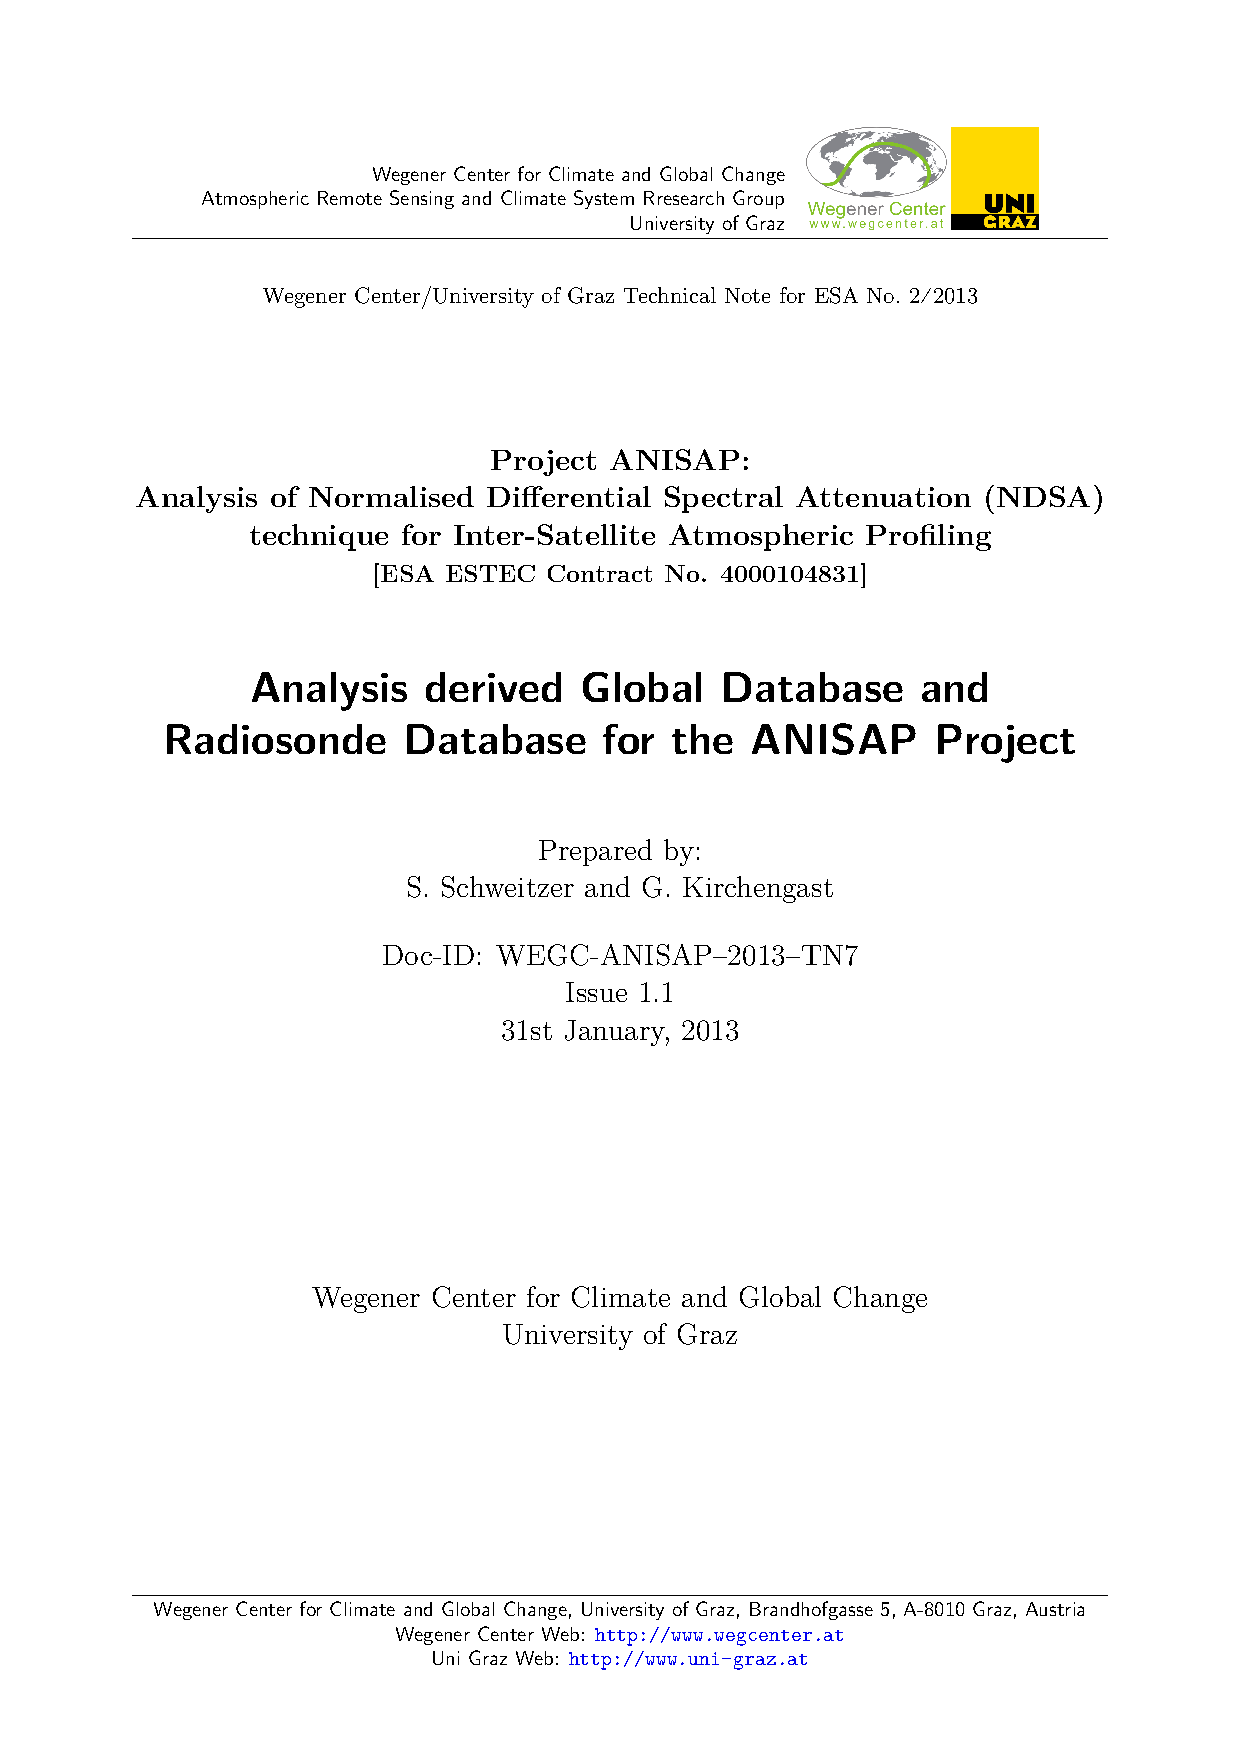
\includegraphics[height=0.7\paperheight, page=1]{anisap-TN2.pdf}}
  \caption{Example of a \multidoc document title page}
  \label{fig:multiDocTitlepage}
\end{figure}

\begin{figure}
  \centering
  \fbox{\includegraphics[height=0.7\paperheight, page=2]{anisap-TN2.pdf}}
  \caption{Example of a \multidoc document release information page}
  \label{fig:multiDocReleaseInfopage}
\end{figure}

\begin{figure}
  \centering
  \fbox{\includegraphics[height=0.7\paperheight, page=3]{anisap-TN2.pdf}}
  \caption{Example of a \multidoc document distribution list page}
  \label{fig:multiDocDistributionList}
\end{figure}

\begin{figure}
  \centering
  \fbox{\includegraphics[height=0.7\paperheight, page=4]{anisap-TN2.pdf}}
  \caption{Example of a \multidoc document change record page}
  \label{fig:multiDocChangeRecord}
\end{figure}

\begin{figure}
  \centering
  \fbox{\includegraphics[height=0.7\paperheight, page=10]{anisap-TN2.pdf}}
  \caption{Example of a \multidoc document random page}
  \label{fig:multiDocHeadings}
\end{figure}



\subsubsection[Document headings]{Tailoring the document headings}
\label{subsubsec:multiDocumentHeadings}

The layout of the document headings (\IE{} the header for the running
pages, see \autoref{fig:multiDocHeadings}) is the same for article, book
and report documents and is structured into three parts:
\begin{enumerate}
\item a four line text block on the left side (the exact definition of the
  concatenation of the string components is given in
  \autoref{lst:docstyleDocumentHeadingsTextBlock}) comprising
  \begin{enumerate}
  \item the document header title (built as a concatenated string from the
    document header title substring \latexcmd{\ThisDocHeaderTitleSubstr}
    and the document subtitle string \latexcmd{\ThisDocSubtitle}
  \item the document identifier (build as a concatenated string from the
    document identifier substring \latexcmd{\ThisDocIdSubstr}, the document
    release year \latexcmd{\ThisDocYear}, the document type%
    \footnote{The acronyms used for the various document types need to be
      defined in the file \path{acronyms.sty}, see
      \fullautoref{subsec:UsingTheAcronymDatabase}.}
    \latexcmd{\ThisDocType} (\EG{} \acs{tr} (\acl{tr}) or \acs{ar}
    (\acl{ar})), and the document internal number
    \latexcmd{\ThisDocIntNum})
  \item the document version (build as a concatenated string from the
    document issue number \latexcmd{\ThisDocIssue} and the document
    revision number \latexcmd{\ThisDocRevision}), and
  \item the document release date
  \end {enumerate}
\item a central single text line indicating the respective current section
  or chapter number and section or chapter title, and
\item a graphics block (of corporate logos) on the right side.
\end{enumerate}

The details and the structure of the document headings are defined in the
file \path{docstyle.sty} near line 315 to 354 (see
\autoref{lst:docstyleDocumentHeadings}).

Since individual details for a specific document from a \multidoc
documentation task are different from document to document due to the
different document content, document type, document identifiers, document
issue, document revision, document release date \ETC{}, these details are
only predefined in the file \path{docstyle.sty}, and intended to be
specifically tailored in each individual document's masterfile.

In essence, a block of redefining \LaTeX{} commands has to be added
(between the two already present commands \latexcmd{\makeatletter} and
\latexcmd{\makeatother}) to the master file, similar to the example given
in \autoref{lst:documentHeadingsExample}.
%
\begin{CommandLineListing}[style=DefaultFileListing, print=true, xleftmargin=0pt, gobble=2, %
  caption={Definition of document headings in the masterfile}, %
  label=lst:documentHeadingsExample]
  \makeatletter

  \renewcommand*{\ThisDocType}{%
    tr%
  }
  \renewcommand*{\ThisDocExtNum}{%
    03%
  }
  \renewcommand*{\ThisDocIntNum}{%
    37%
  }
  \renewcommand*{\ThisDocIssue}{%
    1%
  }
  \renewcommand*{\ThisDocRevision}{%
    3%
  }
  \renewcommand*{\subtitlePrefix}{%
    %
  }
  \renewcommand*{\ThisDocSubtitle}{%
    WLG Quickstart Guide%
  }
  \renewcommand*{\ThisDocHeaderTitleSubstr}{%
    \wegcLaTeX{}%
  }
  \renewcommand*{\ThisDocIdSubstr}{%
    \aces{wegc}-WLG-QSG%
  }
  \newdate{ThisDocDate}{13}{8}{2025}
  \renewcommand*{\ThisDocDate}{%
    \displaydate{ThisDocDate}%
  }
  \renewcommand*{\ThisDocYear}{%
    %% \getdateyear{ThisDocDate}%
    2028%
  }

  \makeatother
\end{CommandLineListing}

\lstinputlisting[style=DefaultFileListing, print=true,
   firstnumber=212, firstline=212, stepnumber=1, lastline=236,
   emptylines=*0,
   breaklines=true,
  caption={Definition of the documents headings text block in \texttt{\lstname}},
  label=lst:docstyleDocumentHeadingsTextBlock]{docstyle.sty}

\begin{landscape}
\lstinputlisting[style=DefaultFileListing, print=true,
   firstnumber=315, firstline=315, stepnumber=1, lastline=354,
   emptylines=*0,
   breaklines=true,
  caption={Definition of the document headings in \texttt{\lstname}},
  label=lst:docstyleDocumentHeadings]{docstyle.sty}
\end{landscape}


\subsubsection[Title page common elements]{Tailoring the common elements of the title page}
\label{subsubsec:multiDocumentTitlePageCommons}

The layout of the document title page is the same for article, book and
report documents and contains elements, which are common and the same for
all documents of a documentation task, \IE{} the title page header, the
title page footer, the document publisher details, the title head and the
subject details, and those that are different due to the individual
document content, \EG{} the document title or the document authors.


\minisec{Title page header and footer}

The common elements title page header and title page footer are defined and
specified in the file \path{docstyle.sty} near lines 252 and 271 (see
\autoref{lst:docstyleTitlepageHeaderFooter}).

\lstinputlisting[style=DefaultFileListing, print=true,
   firstnumber=252, firstline=252, stepnumber=1, lastline=281,
   emptylines=*1,
  caption={Definition of title page header and footer details in \texttt{\lstname}},
  label=lst:docstyleTitlepageHeaderFooter]{docstyle.sty}

If, for example, the combined \ac{igam}/\ac{wegc} title page header and
footer shall be replaced with the plain \ac{wegc} title page header and
footer, then the corresponding section in file \path{docstyle.sty} is to
be modified as shown in
\autoref{lst:docstyleTitlepageHeaderFooterWegcOnly}.
%
\begin{CommandLineListing}[style=DefaultFileListing, print=true, xleftmargin=0pt, gobble=2, %
  caption={Alternate definition of title page header and footer in \latexcmd{docstyle.sty}}, %
  label=lst:docstyleTitlepageHeaderFooterWegcOnly]
  \newcommand*{\Head@@ThisDocTitlePage}{%
    \upshape%
    \begin{varwidth}[b][0pt]{\paperwidth}%
      \LaTeXraggedleft%
      \Name{wegc}\\%
      %% \Name{igam}\\%
      \Name{ug}%
    \end{varwidth}%
    \quad%
    \begin{varwidth}[b][0pt]{\paperwidth}%
      
\includegraphics[height=50.0pt]{logo-ug-medium}%
      \hspace{2.0pt}%
      
\includegraphics[height=50.0pt]{logo-wegc-medium}%
      %% \hspace{2.0pt}%
      %% 
\includegraphics[height=50.0pt]{logo-igam-medium}%
    \end{varwidth}%
  }

  \newcommand*{\Foot@@ThisDocTitlePage}{%
    \upshape%
    \begin{varwidth}[t][0pt]{\paperwidth}%
      \LaTeXcentering%
      \Address{wegc}\\%
      %% \Address{igam}\\%
      \ShortName{wegc} Web\p: \WebAddress{wegc}\\%
      %% \ShortName{igam} Web\p: \WebAddress{igam}\\%
      \ShortName{ug} Web\p: \WebAddress{ug}\\%
    \end{varwidth}%
  }
\end{CommandLineListing}


\minisec{Title head and title subject details}

The title head and title subject details for the title page are defined in
the file \path{docstyle.sty} near lines 444 to 471 (see
\autoref{lst:docstyleTitlepageTitleheadSubject}).

\lstinputlisting[style=DefaultFileListing, print=true,
   firstnumber=444, firstline=444, stepnumber=1, lastline=471,
   emptylines=*0,
   caption={Definition of the title page title head and subject details in \texttt{\lstname}},
   label=lst:docstyleTitlepageTitleheadSubject]{docstyle.sty}

For changing the title page title head and subject details to something
different, the corresponding section in file \path{docstyle.sty} could
be modified as shown in
\autoref{lst:docstyleTitlepageTitleheadSubjectExample}.
%
\begin{CommandLineListing}[style=DefaultFileListing, print=true, xleftmargin=0pt, gobble=2, %
  caption={Alternate definition of title page title head and subject details in \latexcmd{docstyle.sty}}, %
  label=lst:docstyleTitlepageTitleheadSubjectExample]
  \newcommand*{\titleheadSubstr}{%
    \aces{wegc}%
  }
  \newcommand*{\titleheadSubSubstr}{%
    \aces{esa}%
  }
  \titlehead{%
    \makebox[\linewidth]{\titleheadSubstr \hbox{} \acel{\ThisDocType} for \titleheadSubSubstr \hbox{} \No{} \ThisDocExtNum\textfractionsolidus\ThisDocYear}%
  }
  \newcommand*{\subjectStr}{%
    rOPS Project\p:\\%
  }
  \newcommand*{\subjectSubstr}{%
    Typesetting and Document Generation%
  }
  \subject{%
    \subjectStr\subjectSubstr%
  }
\end{CommandLineListing}


\minisec{Publisher information}

The document publisher information for the title page is defined in the
file \path{docstyle.sty} near lines 504 to 520 (see
\autoref{lst:docstyleTitlepagePublisher}).

\lstinputlisting[style=DefaultFileListing, print=true,
   firstnumber=504, firstline=504, stepnumber=1, lastline=520,
   emptylines=*0,
   caption={Definition of the title page publisher details in \texttt{\lstname}},
   label=lst:docstyleTitlepagePublisher]{docstyle.sty}

For changing the title page publisher details to the plain \ac{wegc}
title page publisher details, the corresponding section in file
\path{docstyle.sty} is to be modified as shown in
\autoref{lst:docstyleTitlepagePublisherWegcOnly}.
%
\begin{CommandLineListing}[style=DefaultFileListing, print=true, xleftmargin=0pt, gobble=2, %
  caption={Alternate definition of title publisher details in \latexcmd{docstyle.sty}}, %
  label=lst:docstyleTitlepagePublisherWegcOnly]
  \newcommand*{\publishersSubstr}{%
    \acl{wegc}%
  }
  \newcommand*{\publishersSubSubstr}{%
    \acl{ug}%
  }
  \newcommand*{\publishersSubSubSubstr}{%
    %
  }
  \publishers{%
    \publishersSubstr\\\publishersSubSubstr\\\publishersSubSubSubstr%
  }
\end{CommandLineListing}


\minisec{Glossary and bibliography preambles}

If the default text for the preamble to the \emph{acronyms} and
\emph{abbreviations}, to the \emph{terms} and \emph{definitions}, or to the
bibliography does not fit as expected, these preambles can be modified in
\path{docstyle.sty}, starting near line 657 (see
\autoref{lst:docstyleGlossaryPreambles}) and near line 683 (see
\autoref{lst:docstyleBibliographyPreambles}).

\lstinputlisting[style=DefaultFileListing, print=true,
   firstnumber=657, firstline=657, stepnumber=1, lastline=670,
   emptylines=*0,
   caption={Definition of the glossary preambles in \texttt{\lstname}},
   label=lst:docstyleGlossaryPreambles]{docstyle.sty}

\lstinputlisting[style=DefaultFileListing, print=true,
   firstnumber=683, firstline=683, stepnumber=1, lastline=696,
   emptylines=*0,
   caption={Definition of the bibliography preambles in \texttt{\lstname}},
   label=lst:docstyleBibliographyPreambles]{docstyle.sty}


\subsubsection[Title page specific elements]{Tailoring the document specific elements of the title page}
\label{subsubsec:multiDocumentTitlePageSpecifics}

The layout of the document specific elements document title and authors are
predefined in the file \path{docstyle.sty} and need to be updated in each
individual document's masterfile by a block of redefining \LaTeX{} commands
which are to be added between the two already present commands
\latexcmd{\makeatletter} and \latexcmd{\makeatother}, similar to the
example given in \autoref{lst:documenTitlepageTitleExample}.

All other document specific elements required for the title page like
document type, document identifiers, document issue, document revision,
document release date \ETC{}, have already been described for the document
headings in \autoref{subsubsec:multiDocumentHeadings}

\Attention{%
  In \autoref{lst:documenTitlepageTitleExample}, the definition of the
  document subtitle is not explicitly shown, as it is already presented in
  \autoref{lst:documentHeadingsExample} of
  \autoref{subsubsec:multiDocumentHeadings} (due to the fact that
  \latexcmd{\subtitlePrefix} and \latexcmd{\ThisDocSubtitle} are used for
  the definition of the document headings).}

\begin{CommandLineListing}[style=DefaultFileListing, print=true, xleftmargin=0pt, gobble=2, %
  caption={Definition of document title and author details in the masterfile}, %
  label=lst:documenTitlepageTitleExample]
  \makeatletter
  ...
  ...
  \renewcommand*{\ThisDocTitle}{%
    The \wegcLaTeX{} documentation framework: \newline a guide for beginners%
  }
  \renewcommand*{\titlePrefix}{%
    %
  }
  \renewcommand*{\ThisDocAuthors}{%
    \ShortName{kmf}, \ShortName{jfb}, and \ShortName{gki}%
  }
  \makeatother
\end{CommandLineListing}


\subsubsection[A \multidoc document article]{Creating a \multidoc document article}
\label{subsubsec:creatingMultiDocumentArticle}

For creating a \multidoc article, proceed as follows:
%%
\begin{enumerate}
\item create a working directory for building the \wegcLaTeX{} \multidoc article, \\
  \EG{} \path{/home/\plh{user}/wlMultiDocTest/}

\item create the following subdirectories \\
  \path{/home/\plh{user}/wlMultiDocTest/wlg/}, \\
  \path{/home/\plh{user}/wlMultiDocTest/wlg/figs/}, \\
  \path{/home/\plh{user}/wlMultiDocTest/wlg/data/}, \\
  \path{/home/\plh{user}/wlMultiDocTest/wlg/tex/}, \\
  \path{/home/\plh{user}/wlMultiDocTest/common/}, and \\
  \path{/home/\plh{user}/wlMultiDocTest/common/figs}

  \Attention{Any further documents of a \multidoc documentation task would
    require the additional subdirectories \\
    \path{/home/\plh{user}/wlMultiDocTest/wlg2/}, \\
    \path{/home/\plh{user}/wlMultiDocTest/wlg2/figs/}, \\
    \path{/home/\plh{user}/wlMultiDocTest/wlg2/data/}, \\
    \path{/home/\plh{user}/wlMultiDocTest/wlg2/tex/}, \\
    and so on.}

\item copy the \LaTeX{} template master file \\
  \path{./texmf/doc/latex/wegc-latex/examples/multidoc-article/doc-article.tex} to \\
  \path{/home/\plh{user}/wlMultiDocTest/wlg/}

\item copy the seven \LaTeX{} source code files from \\
  \path{./texmf/doc/latex/wegc-latex/WLG/} to \\
  \path{/home/\plh{user}/wlMultiDocTest/wlg/tex/}

\item copy the twelve \path{*.png} and twelve \path{*.xbb} files from \\
  \path{./texmf/doc/latex/wegc-latex/examples/common/figs/} to \\
  \path{/home/\plh{user}/wlMultiDocTest/common/figs/}

\item copy the three files
  \path{docstyle.sty}, \path{project.sty}, and \path{commands.sty} from \\
  \path{./texmf/doc/latex/wegc-latex/examples/common/} to \\
  \path{/home/\plh{user}/wlMultiDocTest/common}

 \item extract the three example only files \path{acronyms.sty}, \path{addresses.sty}, and
  \path{terms.sty} from the compressed archive file \\
  \path{./texmf/doc/latex/wegc-latex/WLG/acronymsAddressesTerms_ExampleDoNotUse.tar.gz}
  or use the current and up to date versions available at 
  \nolinkurl{https://wegc203117.uni-graz.at/projects/latex_dbs/browser/arsclisys}
  and put them to \\
  \path{/home/\plh{user}/wlMultiDocTest/common}

\item add the address for the fictive person ``\Name{kmf}'' at the end of
  the copied file \path{addresses.sty}, as described in
  \autoref{subsec:usingTheAddressBookDatabase}

\item add the acronym for the fictive company ``\acf{tmc}'' at the end of
  the copied file \path{acronyms.sty}, as described in
  \autoref{subsec:UsingTheAcronymDatabase}

\item add the glossary entry for the fictive term ``\Gls{firlefanzation}''
  at the end of the copied file \path{terms.sty}, as described in
  \autoref{subsec:UsingTheGlossaryDatabase}

\item create an example bibliography file \path{exampleBibFile.bib} in the \\
  \path{/home/\plh{user}/wlMultiDocTest/wlg} directory in the same way as
  it is described for a \singledoc article (see
  \autoref{subsubsec:creatingSingleDocumentArticle})

\item copy the template master file \\
  \path{/home/\plh{user}/wlMultiDocTest/wlg/doc-wlarticle.tex} to \\
  \path{/home/\plh{user}/wlMultiDocTest/wlg/md-wlgArticle.tex} \\
  and apply the following modifications:
  \begin{enumerate}
  \item at line 119, change \latexcmd{DIV=default} to \latexcmd{DIV=11}
  \item between the lines 165 to 171, reading
    \begin{CommandLineListing}[style=DefaultFileListing, print=true, basicstyle={\ttfamily\small}, %
      basewidth=0.47em, xleftmargin=0pt, gobble=6]
      \makeatletter
      %% NOTE: Here, we can act as class and package authors if we want or need to do so ...
      \makeatother
    \end{CommandLineListing}
    add the definition commands for defining the document specific settings:
    \begin{CommandLineListing}[style=DefaultFileListing, print=true, basicstyle={\ttfamily\small}, %
      basewidth=0.47em, xleftmargin=0pt, gobble=6]
      \makeatletter

      \renewcommand*{\ThisDocType}{%
        tr%
      }
      \renewcommand*{\ThisDocExtNum}{%
        03%
      }
      \renewcommand*{\ThisDocIntNum}{%
        37%
      }
      \renewcommand*{\ThisDocIssue}{%
        1%
      }
      \renewcommand*{\ThisDocRevision}{%
        3%
      }
      \renewcommand*{\subtitlePrefix}{%
        %
      }
      \renewcommand*{\ThisDocSubtitle}{%
        WLG Quickstart Guide%
      }
      \renewcommand*{\ThisDocHeaderTitleSubstr}{%
        \wegcLaTeX{}%
      }
      \renewcommand*{\ThisDocIdSubstr}{%
        \aces{wegc}-WLG-QSG%
      }
      \newdate{ThisDocDate}{13}{8}{2025}
      \renewcommand*{\ThisDocDate}{%
        \displaydate{ThisDocDate}%
      }
      \renewcommand*{\ThisDocYear}{%
        %% \getdateyear{ThisDocDate}%
        2028%
      }
      \renewcommand*{\ThisDocTitle}{%
        The \wegcLaTeX{} documentation framework: \newline a guide for beginners%
      }
      \renewcommand*{\titlePrefix}{%
        %
      }
      \renewcommand*{\ThisDocAuthors}{%
        \ShortName{kmf}, \ShortName{jfb}, and \ShortName{gki}%
      }
      \makeatother
    \end{CommandLineListing}

  \item on lines 150 to 151: change from
    \begin{CommandLineListing}[style=DefaultFileListing, print=true, basicstyle={\ttfamily\small}, %
      basewidth=0.47em, xleftmargin=0pt, gobble=6]
      \bibliography{%
      }
    \end{CommandLineListing}
    to
    \begin{CommandLineListing}[style=DefaultFileListing, print=true, basicstyle={\ttfamily\small}, %
      basewidth=0.47em, xleftmargin=0pt, gobble=6]
      \bibliography{%
        exampleBibFile%
      }
    \end{CommandLineListing}

  \item between lines 165 and 171, reading
    \begin{CommandLineListing}[style=DefaultFileListing, print=true, basicstyle={\ttfamily\small}, %
      basewidth=0.47em, xleftmargin=0pt, gobble=6]
      \makeatletter

      %% NOTE: Here, we can act as class and package authors if we want or need to do so ...

      \makeatother
    \end{CommandLineListing}
    add the following command definitiosn for \entity{singledoc} and \entity{multidoc}:
    \begin{CommandLineListing}[style=DefaultFileListing, print=true, basicstyle={\ttfamily\small}, %
      basewidth=0.47em, xleftmargin=0pt, gobble=6]
      \makeatletter

      %% NOTE: Here, we can act as class and package authors if we want or need to do so ...

      \newcommand*{\singledoc}{%
        \entity{singledoc} %
      }

      \newcommand*{\multidoc}{%
        \entity{multidoc} %
      }

      \makeatother
    \end{CommandLineListing}

  \item \label{item:nociteGlsaddIncludeDirectives} between the lines 201
    and 204, reading
    \begin{CommandLineListing}[style=DefaultFileListing, print=true, basicstyle={\ttfamily\small}, %
      basewidth=0.47em, xleftmargin=0pt, gobble=6]
      \printbibliography[prenote=refpreamble]


      \appendix
    \end{CommandLineListing}
    add the following content:
    \begin{CommandLineListing}[style=DefaultFileListing, print=true, basicstyle={\ttfamily\small}, %
      basewidth=0.47em, xleftmargin=0pt, gobble=6]
      \printbibliography[prenote=refpreamble]

      \nocite{Gorbunov2007a}
      \nocite{Gorbunov2002a}
      \nocite{Gorbunov1986}

      \glsadd{development_team}
      \glsadd{firlefanzation}

      \glsadd{urd}
      \glsadd{add}
      \glsadd{ddd}
      \glsadd{sum}
      \glsadd{atr}

      \include{WLG-1_introduction}
      \include{WLG-2_installation}
      \include{WLG-3_documentGeneration}
      \include{WLG-4_commandsAndEnvironments}
      \include{WLG-5_practicalTips}
      \include{WLG-6_usingTheTemplates}
      \include{WLG-7_undocumentedTopics}

      \appendix
    \end{CommandLineListing}
   \end{enumerate}

 \item modify in the file
   \path{/home/\plh{user}/wlMultiDocTest/common/docstyle.sty} the titlepage
   header, titlepage footer, titlehead, subject and publisher details as
   described in \autoref{subsubsec:multiDocumentTitlePageCommons}.

 \item Finally, compile the master file
   \path{/home/\plh{user}/wlMultiDocTest/wlg/md-wlgArticle.tex} as
   described in \autoref{subsec:commandsForDocumentGeneration}.
\end{enumerate}


\subsubsection[A \multidoc document report]{Creating a \multidoc document report}
\label{subsubsec:creatingMultiDocumentReport}

For creating a \multidoc report, copy the \LaTeX{} template master file \\
\path{./texmf/doc/latex/wegc-latex/examples/multidoc-report/doc-report.tex} to \\
\path{/home/\plh{user}/wlMultiDocTest/wlg/}, \\
copy the file \\
\path{/home/\plh{user}/wlMultiDocTest/wlg/doc-wlreport.tex} to \\
\path{/home/\plh{user}/wlMultiDocTest/wlg/md-wlgReport.tex}, \\
and perform all other steps similar to the description in
\autoref{subsubsec:creatingMultiDocumentArticle}, considering the following
differences:
%%
\begin{enumerate}

\item in file \path{/home/\plh{user}/wlMultiDocTest/wlg/md-wlgReport.tex},
  \begin{enumerate}
  \item \label{item:nociteGlsaddIncludeMdReport} between the lines 213 and
    216 (\IE{} between the \latexcmd{\printbibliography} and
    \latexcmd{\appendix} commands), add the same \LaTeX{} commands
    \latexcmd{\nocite}, \latexcmd{\glsadd} and \latexcmd{\include} as
    indicated in \autoref{subsubsec:creatingMultiDocumentArticle},
    \autoref{item:nociteGlsaddIncludeDirectives}

  \item between the lines 213 and 216 (\IE{} between the
    \latexcmd{\printbibliography} and \latexcmd{\appendix} commands and
    immediately after the added statements of
    \autoref{item:nociteGlsaddIncludeMdReport}), add the definition of the
    \entity{Document Release Information} table, the \entity{Document
      Distribution List} and the \entity{Document Change Record}, as shown
    in \autoref{lst:exampleReleaseDistributionChangeRecord}
  \end{enumerate}

\item modify the document structuring directives \latexcmd{\section},
  \latexcmd{\subsection} and \latexcmd{\subsubsection} used in the seven
  \LaTeX{} files to \latexcmd{\chapter}, \latexcmd{\section} and
  \latexcmd{\subsection}, adapting it to the proper sectioning for report
  documents (similar to \autoref{subsubsec:creatingSingleDocumentReport}
  \autoref{item:modifyStructuringDirectives}).

\item Finally, compile the master file
  \path{/home/\plh{user}/wlMultiDocTest/wlg/md-wlgReport.tex} as described
  in \autoref{subsec:commandsForDocumentGeneration}.

\end{enumerate}


\begin{CommandLineListing}[style=DefaultFileListing, print=true, basicstyle={\ttfamily\small}, %
  basewidth=0.47em, xleftmargin=0pt, gobble=2, %
  caption={Definition of document release information, distribution list and change record}, %
  label=lst:exampleReleaseDistributionChangeRecord]
  \renewcommand*{\ThisAuthorizationIdentity}{%
    \ShortName{mip}, \ugorg{short}%
  }

  \renewcommand*{\ThisApprovalIdentity}{%
    \ShortName{gki}, \ugorg{short}%
  }

  %% \renewcommand*{\ThisDocReleaseInformationTab}{%
  %% \ifthenelse{\boolean{KOMAClass}}{\addsec*}{\section*}{Document Release Information}%
  %% \begin{tabularx}{\linewidth}[b]{@{}D@{}}%
  %%   \toprule%
  %%   \docid                                      & \ThisDocId                  \\%
  %%   Issue                                       & \ThisDocVersion             \\%
  %%   Date                                        & \ThisDocDate                \\%
  %%   Prepared by                                 & \ThisDocAuthors             \\%
  %%   Approved\textfractionsolidus{}Internally by & \ThisAuthorizationIdentity  \\%
  %%   Approved\textfractionsolidus{}Externally by & \ThisApprovalIdentity       \\%
  %%   \bottomrule%
  %% \end{tabularx}%
  %% }

  \renewcommand*{\ThisDocDistributionList}{%
    \ShortName{gki}       &  \aces{wegc}/\aces{ug}    & \EmailAddress{gki}       & 1\\%
    \small\ShortName{jfb} &  \aces{wegc}/\aces{ug}    & \small\EmailAddress{jfb} & 1\\%
    \Name{mip}            &  \aces{wegc}/\aces{ug}    & \EmailAddress{mip}       & 1%
  }

  \renewcommand*{\ThisDocChangeRecord}{%
    \software{short}{Version}{1}{0}{}{} &%
    \formatdate{20}{04}{2007} &%
    Original version of the document\p. \\ %
    %%
    \software{short}{Version}{1}{2}{}{} &%
    \formatdate{21}{12}{2008} &%
    Updates throughout the document by minor \newline
    changes and editorial corrections for clarification\p. \\ %
    %%
    \software{short}{Version}{\ThisDocIssue}{\ThisDocRevision}{}{}  &%
    \ThisDocDate &%
    Correction of minor inconsistencies\p.%
  }
\end{CommandLineListing}



\subsubsection[A \multidoc document book]{Creating a \multidoc document book}
\label{subsubsec:creatingMultiDocumentBook}

For creating a \multidoc book, copy the \LaTeX{} template master file \\
\path{./texmf/doc/latex/wegc-latex/examples/multidoc-book/doc-wlbook.tex} to \\
\path{/home/\plh{user}/wlMultiDocTest/wlg/}, copy the file \\
\path{/home/\plh{user}/wlMultiDocTest/wlg/doc-wlbook.tex} to \\
\path{/home/\plh{user}/wlMultiDocTest/wlg/md-wlgBook.tex} 
and perform all other steps similar to the description in
\autoref{subsubsec:creatingMultiDocumentArticle}, considering the following
differences:
%%
\begin{enumerate}

\item in file \path{/home/\plh{user}/wlMultiDocTest/wlg/md-wlgBook.tex},
  \begin{enumerate}
  \item \label{item:nociteGlsaddIncludeMdBook} between the lines 219 and
    222 (\IE{} between the \latexcmd{\mainmatter} and \latexcmd{\appendix}
    commands), add the same \LaTeX{} commands \latexcmd{\nocite},
    \latexcmd{\glsadd} and \latexcmd{\include} as indicated in
    \autoref{subsubsec:creatingMultiDocumentArticle},
    \autoref{item:nociteGlsaddIncludeDirectives}

  \item between the lines 219 and 222 (\IE{} between the
    \latexcmd{\mainmatter} and \latexcmd{\appendix} commands and
    immediately after the added statements of
    \autoref{item:nociteGlsaddIncludeMdBook}), add the definition of the
    \entity{Document Release Information} table, the \entity{Document
      Distribution List} and the \entity{Document Change Record}, as shown
    in \autoref{lst:exampleReleaseDistributionChangeRecord}
  \end{enumerate}

\item modify the document structuring directives \latexcmd{\section},
  \latexcmd{\subsection} and \latexcmd{\subsubsection} used in the seven
  \LaTeX{} files to \latexcmd{\chapter}, \latexcmd{\section} and
  \latexcmd{\subsection}, adapting it to the proper sectioning for book
  documents (similar to \autoref{subsubsec:creatingSingleDocumentReport}
  \autoref{item:modifyStructuringDirectives}).

\item Finally, compile the master file \\
  \path{/home/\plh{user}/wlMultiDocTest/wlg/md-wlgBook.tex} \\
  as described in \autoref{subsec:commandsForDocumentGeneration}.

\end{enumerate}

      


\section[Undocumented topics]{Undocumented topics}

Additionally, the following features are provided as an extension to the \KOMAScript{} bundle:
%
\begin{itemize}
   \item \latexcmd{\rowstyle} and column types \entity{=}, \entity{+}
   \item column type \entity{D}
   \item \latexcmd{\noacronymfont} (\entity{glossaries} package)
   \item \latexcmd{\acrentryshort} (\entity{glossaries} package) and similar commands + shortcuts
\end{itemize}

\noindent{}TODO Describe all packages loaded in \wegcLaTeX{}: What are they
for, basic functionality, basic commands.



      \appendix
    \end{CommandLineListing}

  \item near the lines 135, directly after the \latexcmd{\documentclass}
    directive, add the following commands:
    \begin{CommandLineListing}[style=DefaultFileListing, print=true, basicstyle={\ttfamily\small}, %
      basewidth=0.47em, xleftmargin=0pt, gobble=6]
      \RequirePackage{acronyms}
      \RequirePackage{terms}
      \RequirePackage{addresses}
      \RequirePackage{commands}
    \end{CommandLineListing}

  \end{enumerate}

\item Finally, compile the master file \\
  \path{/home/\plh{user}/wlSingleDocTest/wlg/wlgArticle.tex} \\
  as described in \autoref{subsec:commandsForDocumentGeneration}.
\end{enumerate}


\subsubsection[A \singledoc document report]{Creating a \singledoc document report}
\label{subsubsec:creatingSingleDocumentReport}

For creating a \singledoc report, copy the \LaTeX{} template master file \\
\path{./texmf/doc/latex/wegc-latex/examples/singledoc/master-wlreport.tex} to \\
\path{/home/\plh{user}/wlSingleDocTest/wlg/}. \\
Then copy the file \\
\path{/home/\plh{user}/wlSingleDocTest/wlg/master-wlreport.tex} to \\
\path{/home/\plh{user}/wlSingleDocTest/wlg/wlgReport.tex} \\
and perform all other steps similar to the description in
\autoref{subsubsec:creatingSingleDocumentArticle}, considering the
following differences:
%%
\begin{enumerate}
\item change the setting for \latexcmd{\extratitle},
  \latexcmd{\uppertitleback}, and \latexcmd{\lowertitleback} from
  \begin{CommandLineListing}[style=DefaultFileListing, print=true, basicstyle={\ttfamily\small}, %
    basewidth=0.47em, xleftmargin=0pt, gobble=4]
    \extratitle{%
      \highlight{\placeholder{My Bastard Title}}%
    }
    \uppertitleback{%
      \highlight{\placeholder{My Upper Title Back}}%
    }
    \lowertitleback{%
      \highlight{\placeholder{My Lower Title Back}}%
    }
  \end{CommandLineListing}
  to
  \begin{CommandLineListing}[style=DefaultFileListing, print=true, basicstyle={\ttfamily\small}, %
    basewidth=0.47em, xleftmargin=0pt, gobble=4]
    \extratitle{%
      %
    }
    \uppertitleback{%
      %
    }
    \lowertitleback{%
      %
    }
  \end{CommandLineListing}
  or to specific texts fitting the intended publication.

\item
  instead of
  \begin{CommandLineListing}[style=DefaultFileListing, print=true, basicstyle={\ttfamily\small}, %
    basewidth=0.47em, xleftmargin=0pt, gobble=4]
    \defbibnote{refpreamble}{%
      \highlight{\placeholder{My References Preamble}}%
    }
  \end{CommandLineListing}
  change it to
  \begin{CommandLineListing}[style=DefaultFileListing, print=true, basicstyle={\ttfamily\small}, %
    basewidth=0.47em, xleftmargin=0pt, gobble=4]
    \defbibnote{bibpreamble}{%
      %
    }
  \end{CommandLineListing}
  or to a specific text appropriate for the intended publication.

\item \label{item:modifyStructuringDirectives}
  modify the document structuring directives \latexcmd{\section},
  \latexcmd{\subsection} and \latexcmd{\subsubsection}
  used within the files \\
  \path{WLG-1_introduction}, \\
  \path{WLG-2_installation}, \\
  \path{WLG-3_documentGeneration}, \\
  \path{WLG-4_commandsAndEnvironments}, \\
  \path{WLG-5_practicalTips}, \\
  \path{WLG-6_usingTheTemplates}, and \\
  \path{WLG-7_undocumentedTopics} to \\
  \latexcmd{\chapter}, \latexcmd{\section} and \latexcmd{\subsection},
  adapting it to the proper sectioning for report documents.

\item place the \latexcmd{\include} directives for including the seven
  \LaTeX{} subdocument files between the \latexcmd{\printglossary} and
  \latexcmd{\appendix} commands.

\item Finally, compile the master file \path{wlgReport.tex} as described in
  \autoref{subsec:commandsForDocumentGeneration}.
\end{enumerate}



\subsubsection[A \singledoc document book]{Creating a \singledoc document book}
\label{subsubsec:creatingSingleDocumentBook}

For creating a \singledoc book, copy the \LaTeX{} template master file \\
\path{./texmf/doc/latex/wegc-latex/examples/singledoc/master-wlbook.tex} to \\
\path{/home/\plh{user}/wlSingleDocTest/wlg/}. \\
Then copy the file \\
\path{/home/\plh{user}/wlSingleDocTest/wlg/master-wlbook.tex} to \\
\path{/home/\plh{user}/wlSingleDocTest/wlg/wlgBook.tex} \\
and perform all other steps similar to the description in
\autoref{subsubsec:creatingSingleDocumentArticle}, considering the following differences:
%%
\begin{enumerate}
\item change the settings for \latexcmd{\extratitle},
  \latexcmd{\uppertitleback}, \latexcmd{\lowertitleback},\\
  \latexcmd{\upperinfopage}, \latexcmd{\lowerinfopage}, and
  \latexcmd{\lastpage} from
  \begin{CommandLineListing}[style=DefaultFileListing, print=true, basicstyle={\ttfamily\small}, %
    basewidth=0.47em, xleftmargin=0pt, gobble=4]
    \extratitle{%
      \highlight{\placeholder{My Bastard Title}}%
    }
    \uppertitleback{%
      \highlight{\placeholder{My Upper Title Back}}%
    }
    \lowertitleback{%
      \highlight{\placeholder{My Lower Title Back}}%
    }
    \upperinfopage{%
      \highlight{\placeholder{My Upper Info Page}}%
    }
    \lowerinfopage{%
      \highlight{\placeholder{My Lower Info Page}}%
    }
    \lastpage{%
      \highlight{\placeholder{My Last Page}}%
    }
  \end{CommandLineListing}
  to
  \begin{CommandLineListing}[style=DefaultFileListing, print=true, basicstyle={\ttfamily\small}, %
    basewidth=0.47em, xleftmargin=0pt, gobble=4]
    \extratitle{%
      %
    }
    \uppertitleback{%
      %
    }
    \lowertitleback{%
      %
    }
    \upperinfopage{%
      %
    }
    \lowerinfopage{%
      %
    }
    \lastpage{%
      %
    }
  \end{CommandLineListing}
  or to the specific texts fitting the intended publication.

\item instead of
  \begin{CommandLineListing}[style=DefaultFileListing, print=true,
    basicstyle={\ttfamily\small}, %
    basewidth=0.47em, xleftmargin=0pt, gobble=4]
    \defbibnote{refpreamble}{%
      \highlight{\placeholder{My References Preamble}}%
    }
  \end{CommandLineListing}
  change it to
  \begin{CommandLineListing}[style=DefaultFileListing, print=true,
    basicstyle={\ttfamily\small}, %
    basewidth=0.47em, xleftmargin=0pt, gobble=4]
    \defbibnote{bibpreamble}{%
      %
    }
  \end{CommandLineListing}
  or to a specific text appropriate for the intended publication.

\item modify the document structuring directives \latexcmd{\section},
  \latexcmd{\subsection} and \latexcmd{\subsubsection} used in the seven
  \LaTeX{} files to \latexcmd{\chapter}, \latexcmd{\section} and
  \latexcmd{\subsection}, adapting it to the proper sectioning for book
  documents (similar to \autoref{subsubsec:creatingSingleDocumentReport}
  \autoref{item:modifyStructuringDirectives}).

\item place the \latexcmd{\include} directives for including the seven
  \LaTeX{} subdocument files between the \latexcmd{\mainmatter} and
  \latexcmd{\appendix} commands.

\item finally, compile the master file \path{wlgBook.tex} as described in
  \autoref{subsec:commandsForDocumentGeneration}.

\end{enumerate}



\subsubsection[A \singledoc \ac{msc} or \ac{phd} thesis]{Creating a \singledoc \ac{msc} or \ac{phd} thesis}
\label{subsubsec:creatingMasterOrPhdThesis}

For creating a \singledoc \ac{msc} or \ac{phd} thesis, generally proceed as 
described in the previous \fullautoref{subsubsec:creatingSingleDocumentBook}, 
dealing with a generic \singledoc document book, but change the document title page
similar to the example provided in \autoref{lst:coverPageMasterOrPhdThesis}.  

\begin{CommandLineListing}[style=DefaultFileListing, print=true, basicstyle={\ttfamily\small}, %
                           basewidth=0.47em, xleftmargin=0pt, gobble=3, %
                           caption={Example of a \ac{msc} or \ac{phd} thesis cover page}, %
                           label=lst:coverPageMasterOrPhdThesis]
   %%-------------------------------------------------------------------------%%
   \SetUpPrimaryPageStyle{scrheadings}
   %%
   \renewcommand*{\titlepagestyle}{%
     empty%
   }
   \renewcommand*{\extratitlepagestyle}{%
     empty%
   }
   %%-------------------------------------------------------------------------%%
   %% \extratitle{%
   %%   \highlight{\placeholder{My Bastard Title}}%
   %% }
   %%-------------------------------------------------------------------------%%
   %% \titlehead{%
   %%   \highlight{\placeholder{My Title Head}}%
   %% }
   \subject{%
      \LARGE{Master Thesis} \vspace{2.5mm} \\
      \Large{to obtain the degree Master of Science} \vspace{2.5mm} \\
      \Large{at the Faculty of Natural Sciences} \\
      \Large{University of Graz}%
   }
   %%
   \title{%
     \Huge{Global temperature budget: \\
           Constraints from aircraft and \\
           radio occultation observations}%%
   }
   %%
   \subtitle{%
     %
   }
   %%
   \author{%
     \Large{Franz G. M\"uller, Bakk.rer.nat.}%
   }
   %%
   \date{%
     \large{March 2017}%
     \vspace{5mm}%
   }
   %%
   \publishers{%
      \large{%
      Supervisor: Univ.-Prof.\! Mag.\! Dr.rer.nat.\! Erika L. Mauerheimer%
      \vspace{1.5mm} \\
      Co{\hyphen}Supervisor: Mag.\! Dr.rer.nat.\! Detlef R\"ottbauer}%
      \vspace{7.0mm} \\
      \normalsize{%
      Wegener Center for Climate and Global Change (WEGC) and \\
      Institute for Geophysics, Astrophysics, and
      Meteorology \textfractionsolidus{} Institute of Physics \\
      University of Graz}%
      \vspace{5mm} \\
      
\includegraphics[width=5.5cm]{logo_unigraz_wegc_medium.png}
   }
   %%-------------------------------------------------------------------------%%
   \uppertitleback{%
     %% \highlight{\placeholder{My Upper Title Back}}%
   }
   %%
   \lowertitleback{%
     %% \highlight{\placeholder{My Lower Title Back}}%
   }
   %%-------------------------------------------------------------------------%%
   \upperinfopage{%
     \highlight{\placeholder{My Upper Info Page}}%
   }
   %%
   \lowerinfopage{%
     \highlight{\placeholder{My Lower Info Page}}%
   }
   %%-------------------------------------------------------------------------%%
   \lastpage{%
     \highlight{\placeholder{My Last Page}}%
   }
   %%-------------------------------------------------------------------------%%
   ...
   %% \makeinfopage
   ...
   %%-------------------------------------------------------------------------%%
\end{CommandLineListing}



\subsection[The \multidoc document templates]{Using \multidoc document templates}
\label{subsec:usingMultiDocumentTemplates}

The \multidoc templates are intended for publications that comprise two or
more articles, reports or books and which shall have a common and
consistent layout of the document front matter, \EG{} title page,
distribution list, document revision history, bibliography, lists of
figures and tables as well as document headings.

Sample pages for a \multidoc title page, document release information page,
document distribution list and document change record are provided in
\autoref{fig:multiDocTitlepage}, \autoref{fig:multiDocReleaseInfopage},
\autoref{fig:multiDocDistributionList} and
\autoref{fig:multiDocChangeRecord}.

\begin{figure}
  \centering
  \fbox{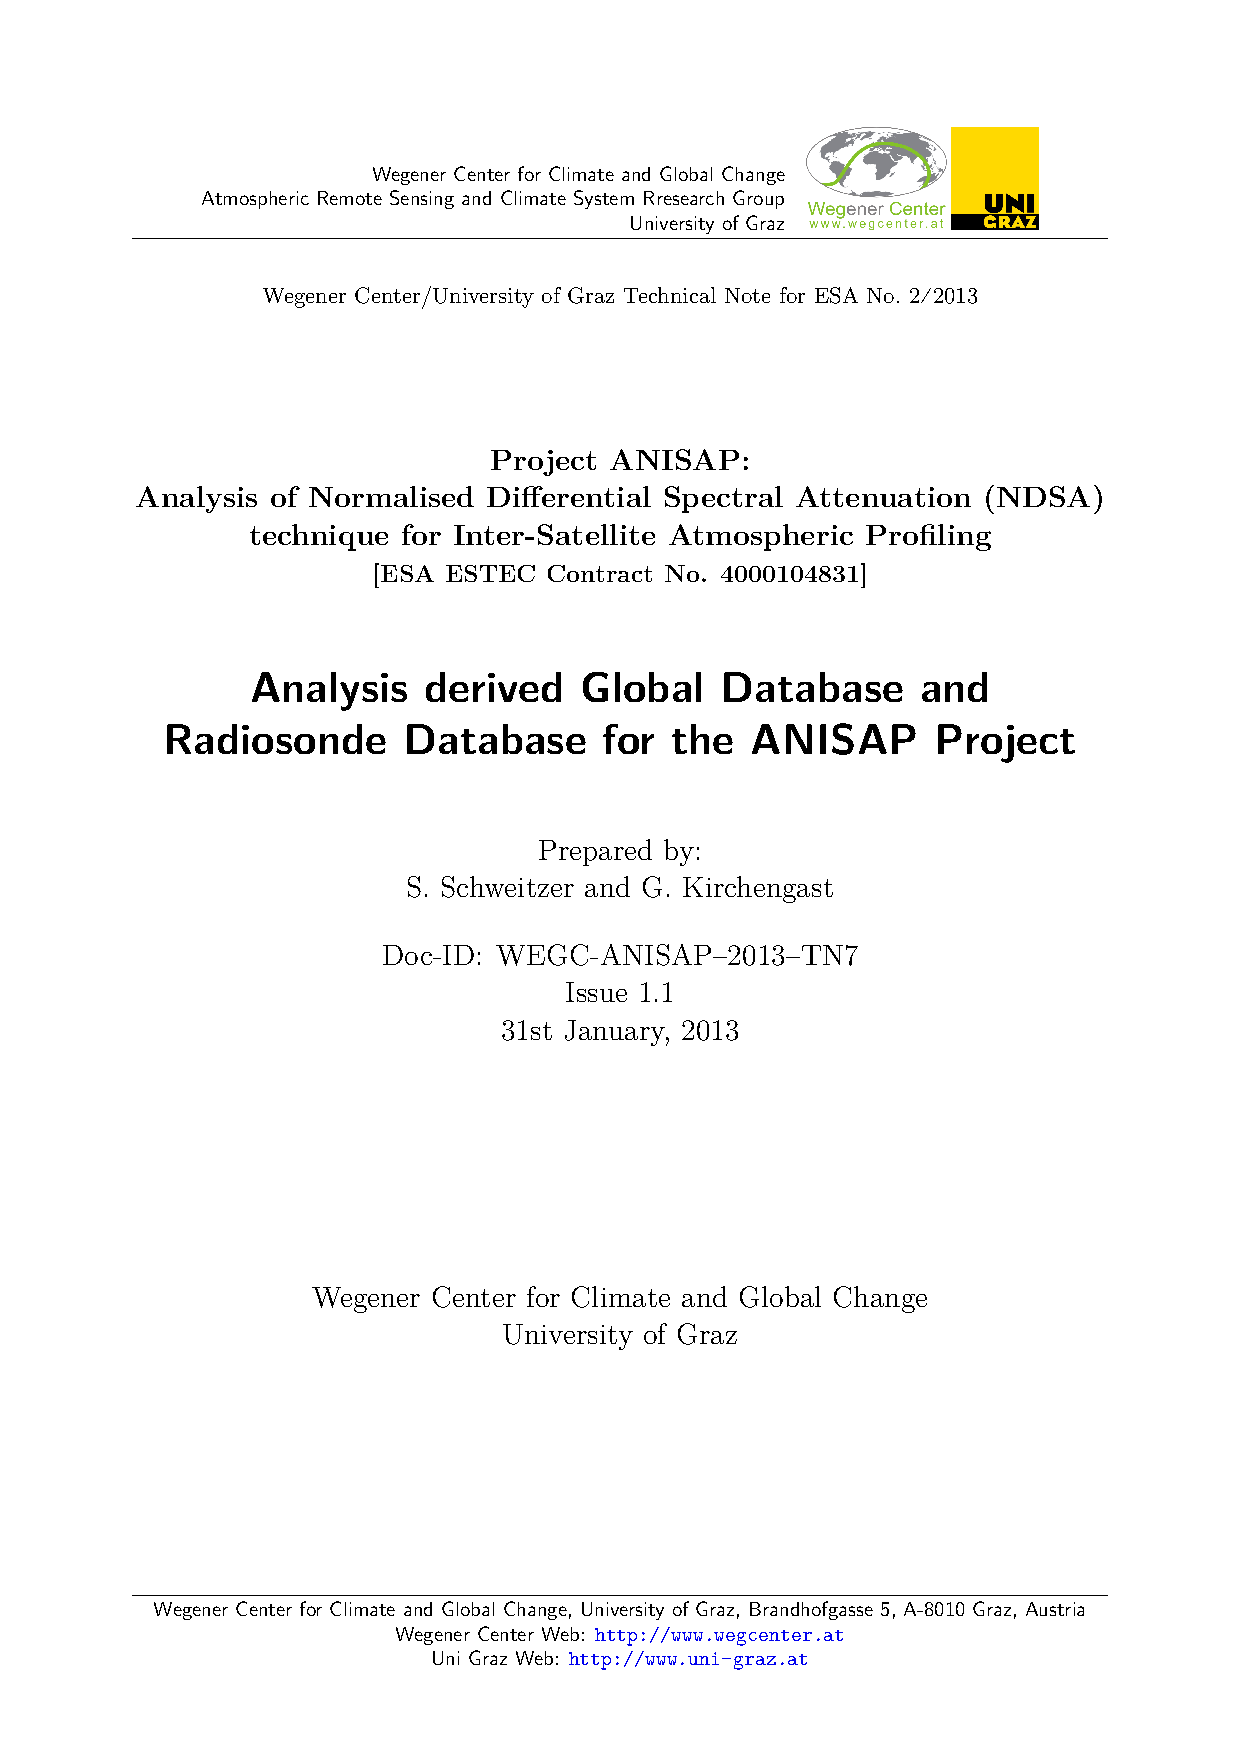
\includegraphics[height=0.7\paperheight, page=1]{anisap-TN2.pdf}}
  \caption{Example of a \multidoc document title page}
  \label{fig:multiDocTitlepage}
\end{figure}

\begin{figure}
  \centering
  \fbox{\includegraphics[height=0.7\paperheight, page=2]{anisap-TN2.pdf}}
  \caption{Example of a \multidoc document release information page}
  \label{fig:multiDocReleaseInfopage}
\end{figure}

\begin{figure}
  \centering
  \fbox{\includegraphics[height=0.7\paperheight, page=3]{anisap-TN2.pdf}}
  \caption{Example of a \multidoc document distribution list page}
  \label{fig:multiDocDistributionList}
\end{figure}

\begin{figure}
  \centering
  \fbox{\includegraphics[height=0.7\paperheight, page=4]{anisap-TN2.pdf}}
  \caption{Example of a \multidoc document change record page}
  \label{fig:multiDocChangeRecord}
\end{figure}

\begin{figure}
  \centering
  \fbox{\includegraphics[height=0.7\paperheight, page=10]{anisap-TN2.pdf}}
  \caption{Example of a \multidoc document random page}
  \label{fig:multiDocHeadings}
\end{figure}



\subsubsection[Document headings]{Tailoring the document headings}
\label{subsubsec:multiDocumentHeadings}

The layout of the document headings (\IE{} the header for the running
pages, see \autoref{fig:multiDocHeadings}) is the same for article, book
and report documents and is structured into three parts:
\begin{enumerate}
\item a four line text block on the left side (the exact definition of the
  concatenation of the string components is given in
  \autoref{lst:docstyleDocumentHeadingsTextBlock}) comprising
  \begin{enumerate}
  \item the document header title (built as a concatenated string from the
    document header title substring \latexcmd{\ThisDocHeaderTitleSubstr}
    and the document subtitle string \latexcmd{\ThisDocSubtitle}
  \item the document identifier (build as a concatenated string from the
    document identifier substring \latexcmd{\ThisDocIdSubstr}, the document
    release year \latexcmd{\ThisDocYear}, the document type%
    \footnote{The acronyms used for the various document types need to be
      defined in the file \path{acronyms.sty}, see
      \fullautoref{subsec:UsingTheAcronymDatabase}.}
    \latexcmd{\ThisDocType} (\EG{} \acs{tr} (\acl{tr}) or \acs{ar}
    (\acl{ar})), and the document internal number
    \latexcmd{\ThisDocIntNum})
  \item the document version (build as a concatenated string from the
    document issue number \latexcmd{\ThisDocIssue} and the document
    revision number \latexcmd{\ThisDocRevision}), and
  \item the document release date
  \end {enumerate}
\item a central single text line indicating the respective current section
  or chapter number and section or chapter title, and
\item a graphics block (of corporate logos) on the right side.
\end{enumerate}

The details and the structure of the document headings are defined in the
file \path{docstyle.sty} near line 315 to 354 (see
\autoref{lst:docstyleDocumentHeadings}).

Since individual details for a specific document from a \multidoc
documentation task are different from document to document due to the
different document content, document type, document identifiers, document
issue, document revision, document release date \ETC{}, these details are
only predefined in the file \path{docstyle.sty}, and intended to be
specifically tailored in each individual document's masterfile.

In essence, a block of redefining \LaTeX{} commands has to be added
(between the two already present commands \latexcmd{\makeatletter} and
\latexcmd{\makeatother}) to the master file, similar to the example given
in \autoref{lst:documentHeadingsExample}.
%
\begin{CommandLineListing}[style=DefaultFileListing, print=true, xleftmargin=0pt, gobble=2, %
  caption={Definition of document headings in the masterfile}, %
  label=lst:documentHeadingsExample]
  \makeatletter

  \renewcommand*{\ThisDocType}{%
    tr%
  }
  \renewcommand*{\ThisDocExtNum}{%
    03%
  }
  \renewcommand*{\ThisDocIntNum}{%
    37%
  }
  \renewcommand*{\ThisDocIssue}{%
    1%
  }
  \renewcommand*{\ThisDocRevision}{%
    3%
  }
  \renewcommand*{\subtitlePrefix}{%
    %
  }
  \renewcommand*{\ThisDocSubtitle}{%
    WLG Quickstart Guide%
  }
  \renewcommand*{\ThisDocHeaderTitleSubstr}{%
    \wegcLaTeX{}%
  }
  \renewcommand*{\ThisDocIdSubstr}{%
    \aces{wegc}-WLG-QSG%
  }
  \newdate{ThisDocDate}{13}{8}{2025}
  \renewcommand*{\ThisDocDate}{%
    \displaydate{ThisDocDate}%
  }
  \renewcommand*{\ThisDocYear}{%
    %% \getdateyear{ThisDocDate}%
    2028%
  }

  \makeatother
\end{CommandLineListing}

\lstinputlisting[style=DefaultFileListing, print=true,
   firstnumber=212, firstline=212, stepnumber=1, lastline=236,
   emptylines=*0,
   breaklines=true,
  caption={Definition of the documents headings text block in \texttt{\lstname}},
  label=lst:docstyleDocumentHeadingsTextBlock]{docstyle.sty}

\begin{landscape}
\lstinputlisting[style=DefaultFileListing, print=true,
   firstnumber=315, firstline=315, stepnumber=1, lastline=354,
   emptylines=*0,
   breaklines=true,
  caption={Definition of the document headings in \texttt{\lstname}},
  label=lst:docstyleDocumentHeadings]{docstyle.sty}
\end{landscape}


\subsubsection[Title page common elements]{Tailoring the common elements of the title page}
\label{subsubsec:multiDocumentTitlePageCommons}

The layout of the document title page is the same for article, book and
report documents and contains elements, which are common and the same for
all documents of a documentation task, \IE{} the title page header, the
title page footer, the document publisher details, the title head and the
subject details, and those that are different due to the individual
document content, \EG{} the document title or the document authors.


\minisec{Title page header and footer}

The common elements title page header and title page footer are defined and
specified in the file \path{docstyle.sty} near lines 252 and 271 (see
\autoref{lst:docstyleTitlepageHeaderFooter}).

\lstinputlisting[style=DefaultFileListing, print=true,
   firstnumber=252, firstline=252, stepnumber=1, lastline=281,
   emptylines=*1,
  caption={Definition of title page header and footer details in \texttt{\lstname}},
  label=lst:docstyleTitlepageHeaderFooter]{docstyle.sty}

If, for example, the combined \ac{igam}/\ac{wegc} title page header and
footer shall be replaced with the plain \ac{wegc} title page header and
footer, then the corresponding section in file \path{docstyle.sty} is to
be modified as shown in
\autoref{lst:docstyleTitlepageHeaderFooterWegcOnly}.
%
\begin{CommandLineListing}[style=DefaultFileListing, print=true, xleftmargin=0pt, gobble=2, %
  caption={Alternate definition of title page header and footer in \latexcmd{docstyle.sty}}, %
  label=lst:docstyleTitlepageHeaderFooterWegcOnly]
  \newcommand*{\Head@@ThisDocTitlePage}{%
    \upshape%
    \begin{varwidth}[b][0pt]{\paperwidth}%
      \LaTeXraggedleft%
      \Name{wegc}\\%
      %% \Name{igam}\\%
      \Name{ug}%
    \end{varwidth}%
    \quad%
    \begin{varwidth}[b][0pt]{\paperwidth}%
      \includegraphics[height=50.0pt]{logo-ug-medium}%
      \hspace{2.0pt}%
      \includegraphics[height=50.0pt]{logo-wegc-medium}%
      %% \hspace{2.0pt}%
      %% \includegraphics[height=50.0pt]{logo-igam-medium}%
    \end{varwidth}%
  }

  \newcommand*{\Foot@@ThisDocTitlePage}{%
    \upshape%
    \begin{varwidth}[t][0pt]{\paperwidth}%
      \LaTeXcentering%
      \Address{wegc}\\%
      %% \Address{igam}\\%
      \ShortName{wegc} Web\p: \WebAddress{wegc}\\%
      %% \ShortName{igam} Web\p: \WebAddress{igam}\\%
      \ShortName{ug} Web\p: \WebAddress{ug}\\%
    \end{varwidth}%
  }
\end{CommandLineListing}


\minisec{Title head and title subject details}

The title head and title subject details for the title page are defined in
the file \path{docstyle.sty} near lines 444 to 471 (see
\autoref{lst:docstyleTitlepageTitleheadSubject}).

\lstinputlisting[style=DefaultFileListing, print=true,
   firstnumber=444, firstline=444, stepnumber=1, lastline=471,
   emptylines=*0,
   caption={Definition of the title page title head and subject details in \texttt{\lstname}},
   label=lst:docstyleTitlepageTitleheadSubject]{docstyle.sty}

For changing the title page title head and subject details to something
different, the corresponding section in file \path{docstyle.sty} could
be modified as shown in
\autoref{lst:docstyleTitlepageTitleheadSubjectExample}.
%
\begin{CommandLineListing}[style=DefaultFileListing, print=true, xleftmargin=0pt, gobble=2, %
  caption={Alternate definition of title page title head and subject details in \latexcmd{docstyle.sty}}, %
  label=lst:docstyleTitlepageTitleheadSubjectExample]
  \newcommand*{\titleheadSubstr}{%
    \aces{wegc}%
  }
  \newcommand*{\titleheadSubSubstr}{%
    \aces{esa}%
  }
  \titlehead{%
    \makebox[\linewidth]{\titleheadSubstr \hbox{} \acel{\ThisDocType} for \titleheadSubSubstr \hbox{} \No{} \ThisDocExtNum\textfractionsolidus\ThisDocYear}%
  }
  \newcommand*{\subjectStr}{%
    rOPS Project\p:\\%
  }
  \newcommand*{\subjectSubstr}{%
    Typesetting and Document Generation%
  }
  \subject{%
    \subjectStr\subjectSubstr%
  }
\end{CommandLineListing}


\minisec{Publisher information}

The document publisher information for the title page is defined in the
file \path{docstyle.sty} near lines 504 to 520 (see
\autoref{lst:docstyleTitlepagePublisher}).

\lstinputlisting[style=DefaultFileListing, print=true,
   firstnumber=504, firstline=504, stepnumber=1, lastline=520,
   emptylines=*0,
   caption={Definition of the title page publisher details in \texttt{\lstname}},
   label=lst:docstyleTitlepagePublisher]{docstyle.sty}

For changing the title page publisher details to the plain \ac{wegc}
title page publisher details, the corresponding section in file
\path{docstyle.sty} is to be modified as shown in
\autoref{lst:docstyleTitlepagePublisherWegcOnly}.
%
\begin{CommandLineListing}[style=DefaultFileListing, print=true, xleftmargin=0pt, gobble=2, %
  caption={Alternate definition of title publisher details in \latexcmd{docstyle.sty}}, %
  label=lst:docstyleTitlepagePublisherWegcOnly]
  \newcommand*{\publishersSubstr}{%
    \acl{wegc}%
  }
  \newcommand*{\publishersSubSubstr}{%
    \acl{ug}%
  }
  \newcommand*{\publishersSubSubSubstr}{%
    %
  }
  \publishers{%
    \publishersSubstr\\\publishersSubSubstr\\\publishersSubSubSubstr%
  }
\end{CommandLineListing}


\minisec{Glossary and bibliography preambles}

If the default text for the preamble to the \emph{acronyms} and
\emph{abbreviations}, to the \emph{terms} and \emph{definitions}, or to the
bibliography does not fit as expected, these preambles can be modified in
\path{docstyle.sty}, starting near line 657 (see
\autoref{lst:docstyleGlossaryPreambles}) and near line 683 (see
\autoref{lst:docstyleBibliographyPreambles}).

\lstinputlisting[style=DefaultFileListing, print=true,
   firstnumber=657, firstline=657, stepnumber=1, lastline=670,
   emptylines=*0,
   caption={Definition of the glossary preambles in \texttt{\lstname}},
   label=lst:docstyleGlossaryPreambles]{docstyle.sty}

\lstinputlisting[style=DefaultFileListing, print=true,
   firstnumber=683, firstline=683, stepnumber=1, lastline=696,
   emptylines=*0,
   caption={Definition of the bibliography preambles in \texttt{\lstname}},
   label=lst:docstyleBibliographyPreambles]{docstyle.sty}


\subsubsection[Title page specific elements]{Tailoring the document specific elements of the title page}
\label{subsubsec:multiDocumentTitlePageSpecifics}

The layout of the document specific elements document title and authors are
predefined in the file \path{docstyle.sty} and need to be updated in each
individual document's masterfile by a block of redefining \LaTeX{} commands
which are to be added between the two already present commands
\latexcmd{\makeatletter} and \latexcmd{\makeatother}, similar to the
example given in \autoref{lst:documenTitlepageTitleExample}.

All other document specific elements required for the title page like
document type, document identifiers, document issue, document revision,
document release date \ETC{}, have already been described for the document
headings in \autoref{subsubsec:multiDocumentHeadings}

\Attention{%
  In \autoref{lst:documenTitlepageTitleExample}, the definition of the
  document subtitle is not explicitly shown, as it is already presented in
  \autoref{lst:documentHeadingsExample} of
  \autoref{subsubsec:multiDocumentHeadings} (due to the fact that
  \latexcmd{\subtitlePrefix} and \latexcmd{\ThisDocSubtitle} are used for
  the definition of the document headings).}

\begin{CommandLineListing}[style=DefaultFileListing, print=true, xleftmargin=0pt, gobble=2, %
  caption={Definition of document title and author details in the masterfile}, %
  label=lst:documenTitlepageTitleExample]
  \makeatletter
  ...
  ...
  \renewcommand*{\ThisDocTitle}{%
    The \wegcLaTeX{} documentation framework: \newline a guide for beginners%
  }
  \renewcommand*{\titlePrefix}{%
    %
  }
  \renewcommand*{\ThisDocAuthors}{%
    \ShortName{kmf}, \ShortName{jfb}, and \ShortName{gki}%
  }
  \makeatother
\end{CommandLineListing}


\subsubsection[A \multidoc document article]{Creating a \multidoc document article}
\label{subsubsec:creatingMultiDocumentArticle}

For creating a \multidoc article, proceed as follows:
%%
\begin{enumerate}
\item create a working directory for building the \wegcLaTeX{} \multidoc article, \\
  \EG{} \path{/home/\plh{user}/wlMultiDocTest/}

\item create the following subdirectories \\
  \path{/home/\plh{user}/wlMultiDocTest/wlg/}, \\
  \path{/home/\plh{user}/wlMultiDocTest/wlg/figs/}, \\
  \path{/home/\plh{user}/wlMultiDocTest/wlg/data/}, \\
  \path{/home/\plh{user}/wlMultiDocTest/wlg/tex/}, \\
  \path{/home/\plh{user}/wlMultiDocTest/common/}, and \\
  \path{/home/\plh{user}/wlMultiDocTest/common/figs}

  \Attention{Any further documents of a \multidoc documentation task would
    require the additional subdirectories \\
    \path{/home/\plh{user}/wlMultiDocTest/wlg2/}, \\
    \path{/home/\plh{user}/wlMultiDocTest/wlg2/figs/}, \\
    \path{/home/\plh{user}/wlMultiDocTest/wlg2/data/}, \\
    \path{/home/\plh{user}/wlMultiDocTest/wlg2/tex/}, \\
    and so on.}

\item copy the \LaTeX{} template master file \\
  \path{./texmf/doc/latex/wegc-latex/examples/multidoc-article/doc-article.tex} to \\
  \path{/home/\plh{user}/wlMultiDocTest/wlg/}

\item copy the seven \LaTeX{} source code files from \\
  \path{./texmf/doc/latex/wegc-latex/WLG/} to \\
  \path{/home/\plh{user}/wlMultiDocTest/wlg/tex/}

\item copy the twelve \path{*.png} and twelve \path{*.xbb} files from \\
  \path{./texmf/doc/latex/wegc-latex/examples/common/figs/} to \\
  \path{/home/\plh{user}/wlMultiDocTest/common/figs/}

\item copy the three files
  \path{docstyle.sty}, \path{project.sty}, and \path{commands.sty} from \\
  \path{./texmf/doc/latex/wegc-latex/examples/common/} to \\
  \path{/home/\plh{user}/wlMultiDocTest/common}

 \item extract the three example only files \path{acronyms.sty}, \path{addresses.sty}, and
  \path{terms.sty} from the compressed archive file \\
  \path{./texmf/doc/latex/wegc-latex/WLG/acronymsAddressesTerms_ExampleDoNotUse.tar.gz}
  or use the current and up to date versions available at 
  \nolinkurl{https://wegc203117.uni-graz.at/projects/latex_dbs/browser/arsclisys}
  and put them to \\
  \path{/home/\plh{user}/wlMultiDocTest/common}

\item add the address for the fictive person ``\Name{kmf}'' at the end of
  the copied file \path{addresses.sty}, as described in
  \autoref{subsec:usingTheAddressBookDatabase}

\item add the acronym for the fictive company ``\acf{tmc}'' at the end of
  the copied file \path{acronyms.sty}, as described in
  \autoref{subsec:UsingTheAcronymDatabase}

\item add the glossary entry for the fictive term ``\Gls{firlefanzation}''
  at the end of the copied file \path{terms.sty}, as described in
  \autoref{subsec:UsingTheGlossaryDatabase}

\item create an example bibliography file \path{exampleBibFile.bib} in the \\
  \path{/home/\plh{user}/wlMultiDocTest/wlg} directory in the same way as
  it is described for a \singledoc article (see
  \autoref{subsubsec:creatingSingleDocumentArticle})

\item copy the template master file \\
  \path{/home/\plh{user}/wlMultiDocTest/wlg/doc-wlarticle.tex} to \\
  \path{/home/\plh{user}/wlMultiDocTest/wlg/md-wlgArticle.tex} \\
  and apply the following modifications:
  \begin{enumerate}
  \item at line 119, change \latexcmd{DIV=default} to \latexcmd{DIV=11}
  \item between the lines 165 to 171, reading
    \begin{CommandLineListing}[style=DefaultFileListing, print=true, basicstyle={\ttfamily\small}, %
      basewidth=0.47em, xleftmargin=0pt, gobble=6]
      \makeatletter
      %% NOTE: Here, we can act as class and package authors if we want or need to do so ...
      \makeatother
    \end{CommandLineListing}
    add the definition commands for defining the document specific settings:
    \begin{CommandLineListing}[style=DefaultFileListing, print=true, basicstyle={\ttfamily\small}, %
      basewidth=0.47em, xleftmargin=0pt, gobble=6]
      \makeatletter

      \renewcommand*{\ThisDocType}{%
        tr%
      }
      \renewcommand*{\ThisDocExtNum}{%
        03%
      }
      \renewcommand*{\ThisDocIntNum}{%
        37%
      }
      \renewcommand*{\ThisDocIssue}{%
        1%
      }
      \renewcommand*{\ThisDocRevision}{%
        3%
      }
      \renewcommand*{\subtitlePrefix}{%
        %
      }
      \renewcommand*{\ThisDocSubtitle}{%
        WLG Quickstart Guide%
      }
      \renewcommand*{\ThisDocHeaderTitleSubstr}{%
        \wegcLaTeX{}%
      }
      \renewcommand*{\ThisDocIdSubstr}{%
        \aces{wegc}-WLG-QSG%
      }
      \newdate{ThisDocDate}{13}{8}{2025}
      \renewcommand*{\ThisDocDate}{%
        \displaydate{ThisDocDate}%
      }
      \renewcommand*{\ThisDocYear}{%
        %% \getdateyear{ThisDocDate}%
        2028%
      }
      \renewcommand*{\ThisDocTitle}{%
        The \wegcLaTeX{} documentation framework: \newline a guide for beginners%
      }
      \renewcommand*{\titlePrefix}{%
        %
      }
      \renewcommand*{\ThisDocAuthors}{%
        \ShortName{kmf}, \ShortName{jfb}, and \ShortName{gki}%
      }
      \makeatother
    \end{CommandLineListing}

  \item on lines 150 to 151: change from
    \begin{CommandLineListing}[style=DefaultFileListing, print=true, basicstyle={\ttfamily\small}, %
      basewidth=0.47em, xleftmargin=0pt, gobble=6]
      \bibliography{%
      }
    \end{CommandLineListing}
    to
    \begin{CommandLineListing}[style=DefaultFileListing, print=true, basicstyle={\ttfamily\small}, %
      basewidth=0.47em, xleftmargin=0pt, gobble=6]
      \bibliography{%
        exampleBibFile%
      }
    \end{CommandLineListing}

  \item between lines 165 and 171, reading
    \begin{CommandLineListing}[style=DefaultFileListing, print=true, basicstyle={\ttfamily\small}, %
      basewidth=0.47em, xleftmargin=0pt, gobble=6]
      \makeatletter

      %% NOTE: Here, we can act as class and package authors if we want or need to do so ...

      \makeatother
    \end{CommandLineListing}
    add the following command definitiosn for \entity{singledoc} and \entity{multidoc}:
    \begin{CommandLineListing}[style=DefaultFileListing, print=true, basicstyle={\ttfamily\small}, %
      basewidth=0.47em, xleftmargin=0pt, gobble=6]
      \makeatletter

      %% NOTE: Here, we can act as class and package authors if we want or need to do so ...

      \newcommand*{\singledoc}{%
        \entity{singledoc} %
      }

      \newcommand*{\multidoc}{%
        \entity{multidoc} %
      }

      \makeatother
    \end{CommandLineListing}

  \item \label{item:nociteGlsaddIncludeDirectives} between the lines 201
    and 204, reading
    \begin{CommandLineListing}[style=DefaultFileListing, print=true, basicstyle={\ttfamily\small}, %
      basewidth=0.47em, xleftmargin=0pt, gobble=6]
      \printbibliography[prenote=refpreamble]


      \appendix
    \end{CommandLineListing}
    add the following content:
    \begin{CommandLineListing}[style=DefaultFileListing, print=true, basicstyle={\ttfamily\small}, %
      basewidth=0.47em, xleftmargin=0pt, gobble=6]
      \printbibliography[prenote=refpreamble]

      \nocite{Gorbunov2007a}
      \nocite{Gorbunov2002a}
      \nocite{Gorbunov1986}

      \glsadd{development_team}
      \glsadd{firlefanzation}

      \glsadd{urd}
      \glsadd{add}
      \glsadd{ddd}
      \glsadd{sum}
      \glsadd{atr}

      
\section[Introduction]{Introduction}
\label{sec:introduction}



\subsection[Scope]{Scope}
\label{subsec:scope}

The intention of this document\footnote{The document in hand is applicable
  to \software{long}{\wegcLaTeX}{0}{9}{5}{200}\p.} is to give new users of
the \wegcLaTeX{} documentation framework a quick introduction on how to use
it in the most efficient way.

Included in this manual are a series of examples on how to create the document layout and how to
use the capabilities of the automatically included \LaTeX{} packages.
No special treatment for typesetting formulas, diagrams or tables is given, as literature
on these topics is readily available.
To a minor extent, it also covers advanced topics mainly relevant to people who want to use \wegcLaTeX{}
within the scope of documentation tasks.

It must be emphasized that it is far beyond the scope of this user guide to address questions about
standard \LaTeX{} concepts. Using \LaTeX{} in a reasonably correct manner is \emph{not} a trivial task.
In fact, it is easy to use it quite wrongly.
It is expected that the reader has a basic understanding on how to create simple \LaTeX{} documents.
So if you are new to \LaTeX{} and/or have never worked in a \LaTeX{} documentation task,
please refer to introductory literature on \LaTeX{}.

At the minimum, you should read %
\textquote[\ctanurl{/tex-archive/info/lshort/english/lshort.pdf}]{%
  The Not So Short Introduction to \LaTeXe%
} %
which provides a very good survey of contemporary \LaTeX{} for both beginners and advanced users.
Nevertheless, it is recommended to study the following documents in some detail:
%
\begin{itemize}
   \item \textquote[]{\LaTeXe{} for authors}
         \footnote{\ctanurl{/tex-archive/macros/latex/doc/usrguide.pdf}}

   \item \textquote[]{An essential guide to \LaTeXe{} usage}
         \footnote{\ctanurl{/tex-archive/info/l2tabu/english/l2tabuen.pdf}}

   \item \textquote[]{\KOMAScript}
         \footnote{\ctanurl{/tex-archive/macros/latex/contrib/koma-script/doc/scrguide.pdf}}

   \item \textquote[]{Math mode}
         \footnote{\url{ftp://ftp.tex.ac.uk/tex-archive/info/math/voss/mathmode/Mathmode.pdf}}

   \item \textquote[]{Using Imported Graphics in \LaTeX{} and pdf\LaTeX}
         \footnote{\ctanurl{/tex-archive/info/epslatex/english/epslatex.pdf}}
\end{itemize}
%
Finally, download and print out the %
\textquote[\url{http://www.stdout.org/~winston/latex/latexsheet.pdf}]{%
  \LaTeXe{} Cheat Sheet%
} %
since this may serve as a handy means for everyday work with \LaTeX.

\wegcLaTeX{} has been developed and is maintained by \Name{mip}. In case of
any questions about \wegcLaTeX{}, please write an email to
\EmailAddress{mip}.



\subsection{Capabilities of \wegcLaTeX{}}
\label{subsec:capabilities}

So, what is the \wegcLaTeX{} documentation framework?
Stated in the most simple way, \wegcLaTeX{} provides an environment for generating documents with a
consistent look and feel. The consistency of the the documents is ensured by providing mechanisms
for consistent usage of common items like names, addresses, email addresses, web addresses, telephone numbers,
abbreviations, acronyms, terms and last but not least, a common and consistent document style for
\singledoc and \multidoc documents.

\smallskip

\singledoc documents have a traditional \LaTeX{} styling, whereas \multidoc
documents are intended for publications that comprise two or more articles,
reports or books, which shall all share a common and consistent layout of
the document front matter, \EG{} title page, distribution list and document
revision history as well as document headings. For a few sample pages of a
\multidoc document, please see \autoref{fig:multiDocTitlepage},
\autoref{fig:multiDocReleaseInfopage},
\autoref{fig:multiDocDistributionList}, \autoref{fig:multiDocChangeRecord}
and \autoref{fig:multiDocHeadings} in
\fullautoref{subsec:usingMultiDocumentTemplates}.

The documents written with \wegcLaTeX{} can be, for example, the
documentation tree associated with a software package, the manual and
handbook set for operating and maintenance procedures of any type of machinery, 
or single documents like \ac{msc} and \ac{phd} theses 
(please see \fullautoref{subsubsec:creatingMasterOrPhdThesis} for an expample),
scientific or technical reports, or papers.

\wegcLaTeX{} provides the means to ensure the consistent layout of the
documents by providing templates for the layout of front matter pages,
title page, distribution list, document revision history, bibliography, as
well as of the lists of figures and tables.

Due to the fact that \wegcLaTeX{} also automatically imports a series of
handy \LaTeX{} packages for the creation and inclusion of external
pictures, diagrams, verbatim text and pretty-printed source code listings,
the user does not need to load any extra packages, but can simply start
writing his or her documentation, taking the provided example documents as
a starting point.

As its name implies, \wegcLaTeX{} is written in the \LaTeX{} document
markup language which is widely used by scientists and other professionals
in both the academic and commercial world.  Distributed under the terms of
the \ac{lppl}, \LaTeX{} is free software.%
\footnote{%
  This statement has sometimes been questioned (\CF{}
  \url{http://en.wikipedia.org/wiki/LPPL}).%
} %
Owing to its platform independence, it can moreover be used in a similar
way on Linux, \ac{mac_os_x}, and Windows machines.

Contemporary \TeX/\LaTeX{} distributions such as \TeXLive{} and \MiKTeX{}
ship with a considerable variety of modules whose capabilities go far
beyond the potentials originally foreseen by the venerable \TeX{}
typesetting system and the \LaTeX{} kernel built on it. In fact, assuming
you are an experienced and sufficiently persistent \LaTeX{} user, you
should nowadays be able to cope with most tasks that might arise while
preparing scientific and/or technical documents.  An incomplete---and, of
course, subjective---list of modules providing the necessary tools for
doing so includes:
%
\begin{labeling}[→]{\KOMAScript{} bundle}
   \item[\KOMAScript{} bundle]%
      modern and highly configurable replacement for the standard \LaTeX{}
      document classes, sophisticated interface for configuring the document
      layout including page style design%
      \footnote{\ctanurl{/tex-archive/macros/latex/contrib/koma-script/doc/scrguide.pdf}}
   \item[\entity{babel} package]%
      multilingual support%
      \footnote{\ctanurl{/tex-archive/macros/latex/required/babel/base/babel.pdf}}
   \item[\entity{url} package]%
      formatting \acp{url}, email addresses, filenames, etc.%
      \footnote{\ctanurl{/tex-archive/macros/latex/contrib/url/url.pdf}}
   \item[\entity{siunitx} package]%
      formatting units of physical quantities%
      \footnote{\ctanurl{/tex-archive/macros/latex/contrib/siunitx/siunitx.pdf}}
   \item[\entity{amsmath} package]%
      high‐quality typesetting of mathematical formulae%
      \footnote{\ctanurl{/tex-archive/macros/latex/required/amslatex/math/amsldoc.pdf}}
   \item[\entity{array} package]%
      replacement for the standard \LaTeX{} tables and arrays%
      \footnote{\ctanurl{/tex-archive/macros/latex/required/tools/array.pdf}}
   \item[\entity{booktabs} package]%
      assistance in producing publication‐quality tables%
      \footnote{\ctanurl{/tex-archive/macros/latex/contrib/booktabs/booktabs.pdf}}
   \item[\entity{longtable} package]%
      creating multipage tables%
      \footnote{\ctanurl{/tex-archive/macros/latex/required/tools/longtable.pdf}}
   \item[\entity{xcolor} package]%
      colour support%
      \footnote{\ctanurl{/tex-archive/macros/latex/contrib/xcolor/xcolor.pdf}}
   \item[\entity{graphicx} package]%
      embedding external graphics given in various formats%
      \footnote{\ctanurl{/tex-archive/macros/latex/required/graphics/grfguide.pdf}}
   \item[\entity{pgf} package]%
      creating graphics%
      \footnote{\ctanurl{/tex-archive/graphics/pgf/base/doc/generic/pgf/pgfmanual.pdf}}
   \item[\entity{mhchem} package]%
      chemical formulae%
      \footnote{\ctanurl{/tex-archive/macros/latex/contrib/mhchem/mhchem.pdf}}
   \item[\entity{listings} package]%
      pretty-printing of source code%
      \footnote{\ctanurl{/tex-archive/macros/latex/contrib/listings/listings.pdf}}
   \item[\entity{glossaries} package]%
      maintaining glossaries, lists of acronyms, indices, etc.\ with
      assistance of the \path{makeindex} program%
      \footnote{\ctanurl{/tex-archive/macros/latex/contrib/glossaries/glossaries-user.pdf}}
   \item[\entity{biblatex} package]%
      maintaining bibliographies based on \BibTeX{} bibliographic database
      files with assistance of the \path{bibtex8} program%
      \footnote{\label{fnote:biblatex}\ctanurl{/tex-archive/macros/latex/exptl/biblatex/doc/biblatex.pdf}}
   \item[\entity{hyperref} package]%
      support for hyperlinks, \ac{pdf} bookmarks, \ac{pdf} document
      information, etc.%
      \footnote{\ctanurl{/tex-archive/macros/latex/contrib/hyperref/doc/manual.pdf}}
   \item[\entity{pdfpages} package]%
      support for inclusion of excerpts from \ac{pdf} documents, etc.%
      \footnote{\ctanurl{/tex-archive/macros/latex/contrib/pdfpages/pdfpages.pdf}}
\end{labeling}


Since 2008, \wegcLaTeX{}, a general purpose document preparation
framework, selects, configures, patches, and extends an adequate
subset of \LaTeX{} modules available from \ac{ctan} according to the
needs of a typical user with scientific and/or technical
background. Not surprisingly, the basis of \wegcLaTeX{} is formed by
just those modules outlined in the preceding list.\footnote{Links to
  the documentation of further \LaTeX{} packages used in \wegcLaTeX{}
  are provided with the corresponding \latexcmd{\RequirePackage{}}
  statements in the \path{wltools.sty} and \path{wlsetup.sty} style
  files of the \wegcLaTeX{} framework} To sum up once more, it can be
said that \wegcLaTeX{} represents a highlevel interface to \LaTeX{}
which should enable its user to write comprehensible, consistent,
reader-friendly, flexible, and easily maintainable scientific and/or
technical documents without being forced to spend much time on looking
into more than the (already comprehensive) fundamentals of the
\LaTeX{} document markup language.

      

\section{Installation}
\label{sec:installation}


\subsection{Installation instructions}
\label{sec:installationInstructions}

\wegcLaTeX{} is provided in the repository hosted at
\nolinkurl{svn+ssh://wegc203117.uni-graz.at/var/lib/svn/wegc_latex/}.

The prerequisite for using \wegcLaTeX{} is a properly installed full \TeXLive{} 2012 distribution on a Linux workstation,
\IE{} the following packages:
\begin{description}
   % \item for \entity{SuSE 12.2}: \\
   %    \path{texlive}, \path{texlive-latex}, \path{texlive-bin-latex}, \\
   %    \path{texlive-tools}, \path{texlive-bin-tools}, \path{texlive-doc}, and \path{texlive-fonts-extra}
   \item for \entity{Debian 7}: \\
      \path{texlive}, and \path{texlive-full}
\end{description}

It should be noted at this place that \wegcLaTeX{} has not been tested with
\MiKTeX{} yet. Experience shows, however, that, if any, only minor
compatibility issues are to be expected.

For installing \wegcLaTeX{} it is only necessary to copy the \wegcLaTeX{}
\texmf{} tree to the \path{\plh{InstallDir}/texmf} directory, and to set up
to three environment variables. \path{\plh{InstallDir}} denotes the
directory in which \path{./texmf/} itself resides, \EG{} if the user's home
directory is used, to \path{/home/<userId>/texmf/}.

Assuming a workstation using the \entity{bash} command language
interpreter, as a second and final step, setting the three environment
variables can be done by adding the following three lines to the
\path{.bashrc} login script:
%
\begin{CommandLineListing}[style=DefaultFileListing, print=true, gobble=3]
   export TEXMFHOME=<InstallDir>/texmf
   export TEXINPUTS=.:./\{data,figs,tex\}//:../common//:
   export BIBINPUTS=.:../common//:
\end{CommandLineListing}
%
\begin{itemize}
\item The \cmdline{TEXMFHOME} variable defines the \wegcLaTeX{}
  installation directory. In this example, it is set to
  \cmdline{TEXMFHOME=<InstallDir>/texmf}. This is only necessary if
  \wegcLaTeX{} is installed to a directory other than the user's home
  (\path{/home/<userId>/}) or the system's pre-defined path
  (\path{/usr/local/share/}). The \LaTeX{} interpreter searches these two
  paths automatically and will use \wegcLaTeX{}, if found there, also
  without setting the \cmdline{TEXMFHOME} variable.
\item The \cmdline{TEXINPUTS} variable defines the locations where
  \wegcLaTeX{} searches for required packages, data, figures, or \LaTeX{}
  source code files. This is convenient, since any file in the
  \path{./data/}, \path{./figs/}, \path{./tex/} or \path{./common/}
  subdirectories can then be referred to by its basename instead of its
  (absolute or relative) pathname.
\item The \cmdline{BIBINPUTS} variable defines the locations where
  \wegcLaTeX{} searches for \path{*.bib} files.
\end{itemize}
%
\Attention{%
  You should not forget to replace the example directory names with the
  real directory names of your installation. Moreover, you must
  \enquote{source} your \path{~/.bashrc} (\IE{} by entering \cmdline{source
    ~/.bashrc} on the command line) in order for the modified shell
  environment to come into effect. If you already maintain a personal
  \texmf{} tree in a non‐standard location, say \path{~/pubs/texmf}, ensure
  that the above two commands are interpreted \emph{after} the commands
  setting up the shell environment for your personal \texmf{}
  tree. Otherwise, there is some probability that \wegcLaTeX{} will not get
  what it actually expects \ldots
}


\subsection{\wegcLaTeX{} file structure}
\label{subsec:structure}

All files belonging to the \wegcLaTeX{} framework are stored below the
\path{\plh{InstallDir}/texmf/} directory. \path{\plh{InstallDir}} denotes
the directory in which the \path{./texmf/} itself resides.
%
The file structure follows the concept of a so‐called \texmf{} tree. At first
glance, you might deem this structure unnecessarily complicated. As a
matter of fact, it is, however, most adequate, given that the file search
algorithms included in \TeX⁄\LaTeX{} distributions such as \TeXLive{} and
\MiKTeX{} are definitely designed and optimized for \texmf{} trees.

The subsequent list describes the subdirectories of the \wegcLaTeX{} file structure:
\begin{description}
   \item \path{./texmf/bibtex/} \\
      This directory hosts \entity{biblatex}-related files (\EG, style files).
    \item \path{./texmf/doc/} \\
      This directory contains the \wegcLaTeX{} templates for
      \singledoc and \multidoc documents in the \\
      \path{./texmf/doc/latex/wegc-latex/examples/singledoc/}, \\
      \path{./texmf/doc/latex/wegc-latex/examples/multidoc-article/}, \\
      \path{./texmf/doc/latex/wegc-latex/examples/multidoc-report/}, and \\
      \path{./texmf/doc/latex/wegc-latex/examples/multidoc-book/} \\
      directories, as well as the document command and layout template files in the \\
      \path{./texmf/doc/latex/wegc-latex/examples/common/} directory.
   \item \path{./texmf/doc/latex/wegc-latex/examples/singledoc/} \\
      This directory contains the \singledoc article, report and book document templates, \IE,
      \path{master-wlarticle.tex}, \path{master-wlreport.tex}, and \path{master-wlbook.tex}.
   \item \path{./texmf/doc/latex/wegc-latex/examples/multidoc-article/}, \\
         \path{./texmf/doc/latex/wegc-latex/examples/multidoc-report/}, and \\
          \path{./texmf/doc/latex/wegc-latex/examples/multidoc-book/} \\
      These directories contain \multidoc article, report and book document templates, \IE, \\
      \path{./multidoc-article/doc-article.tex}, \\
      \path{./multidoc-book/doc-book.tex}, and \\
      \path{./multidoc-report/doc-report.tex}. \\
      Each of these three subdirectories also contain a
      \path{./data/},
      \path{./figs/} and
      \path{./tex/} subdirectory for storing ASCII, image and \LaTeX{} files used.
   \item \path{./texmf/doc/latex/wegc-latex/examples/common/} \\
      This directory contains the \singledoc and \multidoc document command and layout template files \\
      \path{./common/commands.sty}, \\      
      \path{./common/docstyle.sty}, and \\
      \path{./common/project.sty}. \\
      The acronyms, terms, and address definition files 
      \path{acronyms.sty},
      \path{addresses.sty}, and
      \path{terms.sty} are also to be put into this directory 
      (example only versions of these files are provided in the compressed archive file
      \path{./texmf/doc/latex/wegc-latex/WLG/acronymsAddressesTerms_ExampleDoNotUse.tar.gz}, 
      whereas current and up to date versions of these files should be obtained from the separate 
      repository hosted at
      \nolinkurl{https://wegc203117.uni-graz.at/projects/latex_dbs/browser/arsclisys}.%%
      \footnote{The common acronyms, terms, and address
        definitions are easily accessed by adding its directory path to the
        \path{TEXINPUTS} environment variable.} \\
      %%
      The subdirectory \\
      \path{./common/figs/} \\
      contains the images used with \multidoc document cover pages and document headers.
   \item \path{./texmf/dvipdfmx/} \\
      This directory hosts configuration files for the \entity{DVIPDFMx} package,
      used for translating the \entity{DVI} format to \entity{PDF}.
   \item \path{./texmf/tex/} \\
      This directory hosts, among others, the automatically included \LaTeX{} modules mentioned previously
      and the \wegcLaTeX{} kernel.
   \item \path{./texmf/tex/<TBD>/documentVersionInfo.tex} \\
      This file contains the revision definitions used by \wegcLaTeX{}
      (intended to be updated by a \path{./configure} or \path{./makeDocument} script).
      The revision definition consists of three entities, \IE{} \\
      \cmdline{documentRevision},
      \cmdline{documentMajorVersion}, and
      \cmdline{documentMinorVersion}:
      %
      \begin{CommandLineListing}[print=true, gobble=6]
         \newcommand*{\documentMajorVersion}{5}
         \newcommand*{\documentMinorVersion}{6}
         \newcommand*{\documentRevision}{3072}
      \end{CommandLineListing}
\end{description}

For easier offline reading, the manuals for the \LaTeX{} packages mentioned
in \fullautoref{subsec:scope}, \fullautoref{subsec:capabilities} and
\fullautoref{subsec:extensionsToTheLatexKernel}, together with this manual
(\path{WLG.pdf}), are provided in the directory \path{./LaTeX_PDFs/} as
\ac{pdf} files (at the same directory level as the \wegcLaTeX{} \texmf{}
tree).



\subsection{Generating this document}
\label{subsec:generatingThisDocument}

Assuming the \wegcLaTeX{} framework is already properly installed (see \autoref{sec:installationInstructions}),
for generating this document, proceed as follows:
%%
\begin{enumerate}
   \item
      create a working directory, \EG{} \path{/home/\plh{user}/wlgDocGen/}
   \item
      checkout the latest version of \wegcLaTeX{} to \path{/home/\plh{user}/wlgDocGen/}
   \item
      change to the directory containing the master file \path{WLG.tex}, \IE{} \\
      \cmdline{cd /home/\plh{user}/wlgDocGen/trunk/texmf/doc/latex/wegc-latex/WLG}
   \item
      execute the script \path{makeWLG}, \IE{} \\
      \cmdline{./makeWLG} \\
      for generating the \entity{PDF} file \path{WLG.pdf}
\end{enumerate}

      
\section{Document generation}
\label{sec:documentGeneration}



\subsection{Commands for document generation}
\label{subsec:commandsForDocumentGeneration}

Assuming that a complete document has been properly written, all the required subdocument \LaTeX{} source code files, data and figure
files are present in the appropriate subdirectories (as described in \autoref{subsec:structure} on \autopageref{subsec:structure}),
and the master \LaTeX{} file is named \path{masterDoc.tex},
then there are 4 steps necessary for generating the print-ready \entity{PDF} document:

\begin{enumerate}

   \item
   \begin{enumerate}
      \item
         \label{item:pdf_mode}
         \cmdline{pdflatex masterDoc} \\
         Generate the output document in \entity{PDF} format by calling
         \pdfTeX{} in \entity{PDF} mode.  In this case,
         \latexcmd{\documentclass} should include the \cmdline{"pdftex"}
         output driver option. This is the recommended (and default) way.
      \item
         \label{item:dvi_mode}
         \cmdline{latex masterDoc && dvipdfmx masterDoc} \\
         Alternatively, generate the output document in \entity{PDF} format by calling either \TeX{} or \pdfTeX{} in \entity{DVI} mode.
         In this case, \latexcmd{\documentclass} should include the \cmdline{"dvipdfmx"} output driver option.
         If \pdfTeX{} is not installed this command replaces the preceding command.
         If \pdfTeX{} is installed it is an alternative to the preceding command, allowing to generate the output document in a way
         closer to how it would be generated by means of the traditional \TeX{} engine.
         Note that this may imply a significantly smaller \entity{PDF} file size.
   \end{enumerate}

   \item
      \label{item:glossaries}
      \cmdline{makeglossaries masterDoc} \\
      Generate \LaTeX{} code for formatting the glossary sections. Which
      index processor is internally called by the makeglossaries program
      depends on the value of the \cmdline{"glossaries/processor"}
      \latexcmd{\documentclass} option.  It can be \cmdline{"makeindex"} or
      \cmdline{"xindy"}. Default is \cmdline{"makeindex"}.

   \item
   \begin{enumerate}
      \item
         \label{item:bibliographyBT8}
         \cmdline{bibtex8 -c <csfile> -W masterDoc} \\
         Generate \LaTeX{} code for formatting the bibliography section by
         means of the \cmdline{bibtex8} program.  In this case,
         \latexcmd{\documentclass} should set the
         \cmdline{"biblatex/backend"} option to \cmdline{"bibtex8"} (this
         is the default). \cmdline{<csfile>} denotes a \BibTeX{} character
         set and sort definition file such as \path{ascii.csf},
         \path{latin1.csf} or \path{latin9.csf}.  This should match the
         encoding of the bibliographic database. Usually you do not need to
         explicitly set the \cmdline{<csfile>}, leaving you with the
         recommended way of formatting the bibliography:\\\cmdline{bibtex8
           -W masterDoc}.
      \item
         \label{item:bibliographyBT}
         \cmdline{bibtex masterDoc} \\
         Generate \LaTeX{} code for formatting the bibliography section by
         means of the bibtex program. In this case,
         \latexcmd{\documentclass} should set the
         \cmdline{"biblatex/backend"} option to \cmdline{"bibtex"}.
   \end{enumerate}

 \item Repeat \autoref{item:pdf_mode} or \autoref{item:dvi_mode} two more
   times to get all references and hyperlinks such as
   \latexcmd{\autoref{}}, \latexcmd{\ac{}} and/or \latexcmd{\textcite{}}
   \ETC{} properly updated.

\end{enumerate}

An example script, which uses as first argument the basename of the
\LaTeX{} master file, is presented in
\autoref{lst:documentGenerationScript}. Please note that during your daily
working routine, it is not necessary to perform all these steps; in most
cases, a simple run of \autoref{item:pdf_mode} will update your
\entity{PDF} most efficiently.

\Attention{%
  The more traditional \path{tex}→\path{dvi}→\path{pdf} document generation
  approach listed under \autoref{item:dvi_mode} does not work well at the
  moment because a few \LaTeX{} modules loaded by \wegcLaTeX{}
  insufficiently support the underlying \entity{dvipdfm} driver.
  Furthermore note that the \entity{glossaries} package does not give any
  indication whether \path{makeindex} must be called at a specific stage of
  document generation to update the \enquote{\glossaryname} and
  \enquote{\acronymname} sections as outlined under
  \autoref{item:glossaries}.  Unfortunately, this circumstance makes the
  implementation of an \emph{intelligent} build system a rather challenging
  task.  Assuming the \enquote{\bibname} section is very large and⁄or
  several secondary reference lists exist, calling \path{bibtex8} is likely
  to result in an error despite specifying the high‐capacity
  \path{-W} switch suggested under
  \autoref{item:bibliographyBT8}. If this happens, resort to the
  \entity{biblatex} package documentation (see \autoref{fnote:biblatex})
  which describes in detail how to maximize the capacity of the
  \path{bibtex8} program at run time.}


\begin{CommandLineListing}[style=DefaultFileListing, print=true, basicstyle={\ttfamily\small}, %
                           basewidth=0.47em, xleftmargin=0pt, gobble=3, %
                           caption={Example script for document generation}, %
                           label=lst:documentGenerationScript]
   #! /bin/bash
   export TEXMFHOME=/home/<userId>/texmf
   export TEXINPUTS=.:./\{data,figs,tex\}//:../common//:
   export BIBINPUTS=.:../common//:

   masterDoc=${1}
   latex=pdflatex
   makeglossaries=makeglossaries
   bibtex='bibtex8 -W'
   rm='/bin/rm -f'
   intermediateFiles='*.acn *.acr *.alg *.aux *.bbl *.blg *-blx.bib *.dvi *.glo *.glg *.gls *.ist *.lof *.log *.lol *.lot *.nlg *.noa *.not *.run.xml *.toc'
   ${rm} ${intermediateFiles} &&
   ${latex} ${masterDoc} &&
   ${makeglossaries} ${masterDoc} &&
   ${bibtex} ${masterDoc} &&
   ${latex} ${masterDoc} &&
   ${makeglossaries} ${masterDoc} &&
   ${latex} ${masterDoc} &&
   ${latex} ${masterDoc} &&
   ${rm} ${intermediateFiles}
\end{CommandLineListing}



\subsection{Global Options for document generation}
\label{subsec:globalOptionsForDocumentGeneration}

In \LaTeX{}, global options are specified in the optional argument of the \latexcmd{\documentclass} command which selects the
document class to be used for a document, usually found at the very beginning of a \LaTeX{} master file.
Global options are not only processed by the document class module, but are also taken into account by subsequently loaded packages.
Thus, they provide the primary means for a \LaTeX{} user to change the overall appearance and other global properties of a document.

An example \latexcmd{\documentclass} command setup for use with \wegcLaTeX{} is given in \fullautoref{lst:documentClassExample} and
a short explanation of the \latexcmd{\documentclass} command values is given in \fullautoref{table:documentClassCommandSettings}.


\begin{landscape}
\begin{CommandLineListing}[style=DefaultFileListing, print=true, basicstyle={\ttfamily\small}, %
                           basewidth=0.47em, xleftmargin=0pt, gobble=3, %
                           caption={Example \latexcmd{\documentclass} command settings in the masterfile}, %
                           label=lst:documentClassExample]
   \documentclass[
     %% output driver ("pdftex" when calling pdfLaTeX or "dvipdfmx" when calling LaTeX):
     pdftex,
     %% final or draft document version ("final" or "draft"):
     draft,
     %% web or print document version ("web" or "print"):
     web,
     %% main document language ("english", "USenglish", "UKenglish", "ngerman" or "naustrian"):
     UKenglish,
     %% paper size (ISO 216 paper size, North American paper size, "portrait" or "landscape"):
     paper=a4,
     %% font size (in pt):
     fontsize=11pt,
     %% DIV factor ("default", "calc" or integer >= 4):
     DIV=11,
     %% binding correction (in mm):
     BCOR=0mm,
     %% way of including glossary section headings in the table of contents ("nottotoc", "totoc" or "totocnumberline"):
     glossaries=totoc,
     %% acronym style ("default", "dua", "footnote", "smallcaps", "smaller", "description", "description+dua" or
     %% "description+footnote"):
     glossaries/acronymstyle=default,
     %% index processor used along with the glossaries package ("default", "makeindex" or "xindy"):
     glossaries/processor=makeindex,
     %% bibliography/citation style ("default" or a style known to the biblatex package):
     biblatex/style=default,
     %% bibliographic database backend used along with the biblatex package ("default", "bibtex" or "bibtex8"):
     biblatex/backend=bibtex8,
     %% encoding of the bibliographic database ("default", "auto", "x-ascii", "x-iso-8859-15" or another
     %% single-byte encoding known to the inputenx package):
     biblatex/bibencoding=x-ascii
   ]{wlarticle}[2011/07/26]
\end{CommandLineListing}
\end{landscape}

\begin{longtable}{l p{6.0cm} p{3.0cm}}
   \caption{Available \latexcmd{\documentclass} command settings in the masterfile} %%
   \label{table:documentClassCommandSettings} \\
   \toprule
   Command item        &  possible values                                                      & example setting \\
   \midrule
   document class      & \entity{wlarticle} | \entity{wlbook} | \entity{wlreport}              & \path{wlreport} \\
   output driver       & \entity{pdftex} | \entity{dvipdfmx}                                   & \path{pdftex} \\
   document version    & \entity{final} | \entity{draft}                                       & \path{final} \\
   document type       & \entity{web} | \entity{print}                                         & \path{print} \\
   document language   & \entity{english} | \entity{UKenglish} | \entity{USenglish} | \newline
                         \entity{ngerman} | \entity{naustrian}                                 & \path{UKenglish} \\
   paper size          & \entity{a4} | \entity{a3}                                             & \path{paper=a4} \\
   font size           & \entity{11pt}                                                         & \path{fontsize=11pt} \\
   \entity{DIV} factor & \entity{default} | \entity{calc} | integer >= 4                       & \path{DIV=11} \\
   binding correction  & binding correction (in mm)                                            & \path{BCOR=5mm} \\
   \bottomrule
\end{longtable}


\subsection{Merging subdocuments}
\label{subsec:mergingSubdocuments}

For merging and joining partial documents or subdocuments to a single
\entity{PDF} document, the \entity{multivalent} tool
(\url{http://multivalent.sourceforge.net/}) is highly recommended.  This
Java based tool requires an up to date Sun-Java installation and can be
downloaded\footnote{The file \path{Multivalent20091027.jar} and an older
  version of this tool (\path{Multivalent20060102.jar}) are stored in the
  directory \path{./LaTeX_PDFs/Multivalent/} for ease of access only.}
%%
from the \entity{multivalent} download page at
\url{http://sourceforge.net/projects/multivalent/files/multivalent/Release20091027/Multivalent20091027.jar/}.\\
For joining two \entity{PDF} files, perform the following steps:
%
\begin{CommandLineListing}[print=true, gobble=0]
   cp Multivalent20060102.jar /usr/local/share/java/
   export CLASSPATH=/usr/local/share/java/*
   java tool.pdf.Merge file1.pdf file2.pdf
\end{CommandLineListing}

Note that for simple applications such as adding one or several cover pages
produced by an external tool in \entity{PDF} format, the \entity{pdfpages}
package included in \wegcLaTeX{} (\autoref{subsec:capabilities}) will be a
more appropriate approach. Please refer to the \entity{pdfpages} manual for
further details.

      

\section{Commands and environments}
\label{sec:commandsAndEnvironments}


\subsection{Extensions to the \LaTeX{} kernel}
\label{subsec:extensionsToTheLatexKernel}

\begin{description}
\item[\latexcmd{\hyphen}] \enforcenewline%
  Expands to a hyphen with less restrictive hyphenation properties as
  compared to the primitive \enquote{\latexcmd{-}} character. Using
  \latexcmd{\hyphen} within compound words lowers the risk of getting
  overfull horizontal boxes. \\
  \latexcmd{\hyphen} can also be accessed via the Unicode character at code
  point U+2010.

\item[\latexcmd{\nbhyphen}] \enforcenewline%
  Expands to a non\hyphen{}breaking \latexcmd{\hyphen}. \\
  \latexcmd{\nbhyphen} can also be accessed via the Unicode character at
  code point U+2011.

\item[\latexcmd{\textendash}] \enforcenewline%
  Expands to an en-dash, slightly longer than a hyphen. This command is an
  alternative form to using \enquote{\cmdline{--}} in the \LaTeX{} source
  code, which expands to the same en-dash, but with slightly different
  hyphenation properties. The en-dash is used for ranges, \EG{} ``3--7'',
  and to separate name pairs, for example, the text%
  \begin{CommandLineListing}[print=true, xleftmargin=0pt, gobble=4]%
    ``Euler\textendash{}Lagrange, Stefan\textendash{}Sussmann''
  \end{CommandLineListing}
  gives the output: \\
  ``Euler\textendash{}Lagrange, Stefan\textendash{}Sussmann''. \\
  \latexcmd{\textendash} can also be accessed via the Unicode character at
  code point U+2013. For truly compound names (named after one person),
  such as ``Lennard-Jones'', use the simple hyphen. The en-dash is also
  used in German sentences to mark ``parenthetical comments'' (see
  \latexcmd{\textemdash} for the English style to do this), for example:
  \begin{CommandLineListing}[print=true, xleftmargin=0pt, gobble=4]%
    ``Das Wichtigste \textendash{} wenn du es wirklich wissen m\"ochtest
    \textendash{} ist, Bindestriche richtig einzusetzen.''
  \end{CommandLineListing}
  gives the output: \\
  ``Das Wichtigste \textendash{} wenn du es wirklich wissen m\"ochtest
  \textendash{} ist, Bindestriche richtig einzusetzen.'' \\
  Note that in German a space character is used to separate the en-dash
  from the surrounding words.

\item[\latexcmd{\textemdash}] \enforcenewline%
  Expands to an em-dash, slightly longer than a en-dash. This command is an
  alternative form to using \enquote{\cmdline{---}} in the \LaTeX{} source
  code, which expands to the same em-dash, but with slightly different
  hyphenation properties. Use this type of dash for ``parenthetical
  comments''. For example, the text%
  \begin{CommandLineListing}[print=true, xleftmargin=0pt, gobble=4]%
    ``The main thing\textemdash{}if you must know\textemdash{}is to use
    hyphens properly.''
  \end{CommandLineListing}
  gives the output: \\
  ``The main thing\textemdash{}if you must know\textemdash{}is to use hyphens properly.''\\
  \latexcmd{\textemdash} can also be accessed via the Unicode character at
  code point U+2014. For details about how to use the various types of
  dashes, please refer to \EG{} \url{https://en.wikipedia.org/wiki/Dash}.

\item[\latexcmd{\textminus}] \enforcenewline%
  Use this to indicate negative numbers. For example, the text
  \begin{CommandLineListing}[print=true, xleftmargin=0pt, gobble=4]%
    ``\textminus{}128''
  \end{CommandLineListing}
  gives the following output: \\
  `` \textminus{}128''\\
  \latexcmd{\textminus} can also be accessed via the Unicode character at
  code point U+2212.

\item[\latexcmd{\textfractionsolidus}] \enforcenewline%
  Yields a slash with alternative (perhaps more attractive) typeface. The
  hyphenation properties of \latexcmd{\textfractionsolidus} are less
  restrictive than those shown by the standard \LaTeX{} \latexcmd{\slash}
  command and, thus, help avoid overfull horizontal boxes. Using the
  primitive \enquote{\latexcmd{/}} character in ordinary textual contexts
  is in general deprecated. \\
  \latexcmd{\textfractionsolidus} can also be accessed via the Unicode
  character at code point U+2044.

\item[\latexcmd{\backtextfractionsolidus}] \enforcenewline%
  Expands to a backslash with a typeface similar to
  \latexcmd{\textfractionsolidus}.

\item[\latexcmd{\hardbreak}] \enforcenewline%
  Indicates that a line break at the immediately following space is
  undesirable, but still acceptable.

\item[\latexcmd{\enforcenewline}] \enforcenewline%
  Causes a line break, even at positions where this is normally forbidden
  (\EG{} at the start of a paragraph).

\item[\latexcmd{\p\plh{punctuationMark}}] \enforcenewline%
  Enforces the correct spacing after
  \entity{\plh{punctuationMark}}. \latexcmd{\p} supersedes the standard
  \LaTeX{} \latexcmd{\@} command in that it does not destroy kerning.

\item[\latexcmd{\dokerning{\plh{group_1}}{\plh{token}}{\plh{group_2}}}]
  \enforcenewline%
  Restores the kerning between \entity{\plh{group_1}} and
  \entity{\plh{group_2}} lost because of using \entity{\plh{token}}.

\item[\latexcmd{\SetUpHyphenation[\plh{language}]{\plh{hyphenationRules}}}]
  \enforcenewline%
  Lets you specify additional \entity{\plh{hyphenationRules}} for
  \entity{\plh{language}} or, if \entity{\plh{language}} is omitted, for
  the primary language of the document. The \entity{\plh{hyphenationRules}}
  are specified according to the scheme prescribed by the standard \LaTeX{}
  \latexcmd{\hyphenation} command. Note that \latexcmd{\SetUpHyphenation}
  may only be used in the document preamble.

\item[\latexcmd{\fullautoref{\plh{referenceLabel}}}] \enforcenewline%
  This is an interim replacement for the \latexcmd{\vref{}} command from
  the \entity{varioref}
  package\footnote{\ctanurl{/tex-archive/macros/latex/required/tools/varioref.pdf}}
  (which currently produces some undesired side effects). In addition to
  the output of the recommended \latexcmd{\autoref} command, the page
  number of the reference target is printed with \latexcmd{\fullautoref}.

\item[\latexcmd{\software{\plh{short|long}}{\plh{swName}}{\plh{swMajor}}{\plh{swMinor}}{\plh{swMicro}}{swRev}}]
  \enforcenewline%
  Expands to a software version string, \EG{} \\
  \latexcmd{\software{long}{rOPS}{7}{7}{1}{2111}} $\rightarrow$
  \software{long}{rOPS}{7}{7}{1}{2111}, or \newline
  \latexcmd{\software{short}{rOPS}{7}{8}{}{}} $\rightarrow$
  \software{short}{rOPS}{7}{8}{}{} \p.

\item[\latexcmd{\placeholder{\plh{dummyArgument}}}] \enforcenewline%
  Expands to a string indicating a dummy argument, \EG{} \\
  \latexcmd{\placeholder{telephoneNumber}} $\rightarrow$
  \placeholder{telephoneNumber} \p.

\item[\latexcmd{\plh{\plh{dummyArgument}}}] \enforcenewline%
  A shortcut to the previous command \latexcmd{\placeholder{}} is available as \latexcmd{\plh{}}, \EG{} \\
  \latexcmd{\plh{telephoneNumber}} $\rightarrow$ \plh{telephoneNumber} \p.

\item[\latexcmd{\cmdline{\plh{consoleCommandlineString}}}] \enforcenewline%
  Expands to a verbatim, fixed font printed \plh{consoleCommandlineString} as it is commonly encountered at a console commandline, \EG{} \\
  \latexcmd{\cmdline{tar -xzf data_file.tar.gz}} $\rightarrow$ \cmdline{tar
    -xzf data_file.tar.gz} \p.

\item[\latexcmd{\path{\plh{fileOrDirecoryPathName}}}] \enforcenewline%
  Expands to a verbatim, fixed font printed \path{\plh{fileOrDirecoryPathName}}, similar \\
  to \latexcmd{\cmdline}.

\item[\latexcmd{\entity{\plh{textString}}}] \enforcenewline%
  \latexcmd{\entity} is intended to be used for marking a \plh{textString}
  that represents some form of an entity.  For example, the text
  \latexcmd{\entity{Orion}} will be printed as \entity{Orion}\p.

\item[\latexcmd{\supplement{\plh{textStrings}}}] \enforcenewline%
  Expands to the \plh{textStrings} enclosed in square brackets.  For
  example, the text%
  \begin{CommandLineListing}[print=true, xleftmargin=0pt, gobble=4]%
    ``The data \supplement{and the run control files} reside in the
    \path{/data/RAOB/} directory.''
  \end{CommandLineListing}
  gives the output: \\
  ``The data \supplement{and the run control files} reside in the
  \path{/data/RAOB/} directory.''

   % \item[\latexcmd{\insi{\plh{textStrings}}}] \enforcenewline%
   %    Expands to the \plh{textStrings} enclosed in round brackets.
   %    For example \todo{figure out what the \insi{} is intended for}, the text%
   %    \begin{CommandLineListing}[print=true, xleftmargin=0pt, gobble=4]%
   %       ``I do not know what for \insi{and why} the \latexcmd{\insi} is there.''
   %    \end{CommandLineListing}
   %    gives the output: \\
   %       ``I do not know what for \insi{and why} the \latexcmd{\insi} is there.''
   %% TODO: insi is not working as described here. And I do not know how it works...


\item[\latexcmd{\Attention{\plh{blockOfText}}}] \enforcenewline%
  Expands to a boldface string reading \textbf{Attention:} followed by \plh{blockOfText}. \\
  For example, the text%
  \begin{CommandLineListing}[print=true, xleftmargin=0pt, gobble=4]%
    \Attention{%
      Please note that keeping food near any terminal device
      might cause unpredictable results during program execution!
    }
  \end{CommandLineListing}
  gives the output: \\
  \Attention{%
    Please note that keeping food near any terminal device
    might cause unpredictable results during program execution!
  }

\item[\latexcmd{\highlight{\plh{blockOfText}}}] \enforcenewline%
  Expands to a yellow highlighted \plh{blockOfText}, independent of the document version (\entity{final} | \entity{draft}).
  For example, the text%
  \begin{CommandLineListing}[print=true, xleftmargin=0pt, gobble=4]%
    \highlight{The output values are still unexpected!}
  \end{CommandLineListing}
  gives the output: \\
  \highlight{The output values are still unexpected!}

  \Attention{%
    The \latexcmd{\highlight} command does not automatically produce any linebreaks
    and it is not sensitive to \latexcmd{\enforcenewline} and \latexcmd{\newline} commands.
    As a matter of fact, it can not be used to highlight more than one line of text.
  }

\item[\latexcmd{\todo{\plh{blockOfText}}}] \enforcenewline%
  With a document version \entity{draft}, it expands to a sequentially
  numbered red text \emph{TODO} at the paper margin near the location
  where the \latexcmd{\todo} appears, and a list of \entity{TODOs},
  sequentially numbered, with a page indicator and the associated
  \plh{blockOfText} at the end of the document. With a document version \entity{final}, the \latexcmd{\todo} is completely ignored. \\
  An example \latexcmd{\todo} command could read:%
  \begin{CommandLineListing}[print=true, xleftmargin=0pt, gobble=4]%
    \todo{Table values need to be updated for the latest measurements!}
  \end{CommandLineListing}

\item[\latexcmd{\No{}}, \latexcmd{\CF{}}, \latexcmd{\EG{}}, \latexcmd{\ETC{}}, and \latexcmd{\IE{}}] \enforcenewline%
  \latexcmd{\No{}}, \latexcmd{\CF{}}, \latexcmd{\EG{}}, \latexcmd{\ETC{}}, and \latexcmd{\IE{}}
  are expanded to conveniently formatted strings, \EG{} \newline
  the \latexcmd{\No{}} 4711 is magic           ~ $\rightarrow$ ~  the \No{} 4711 is magic \newline
  is true, \latexcmd{\CF{}} the letter of      ~ $\rightarrow$ ~  is true, \CF{} the letter of \newline
  is false, \latexcmd{\EG{}} in the case of    ~ $\rightarrow$ ~  is false, \EG{} in the case of \newline
  mist, smoke, \latexcmd{\ETC{}} in air.       ~ $\rightarrow$ ~  mist, smoke, \ETC{} in air. \newline
  is always the case, \latexcmd{\IE{}} true.   ~ $\rightarrow$ ~  is always the case, \IE{} true.

\item[\latexcmd{\pdfTeX{}}, \latexcmd{\pdfLaTeX{}}, \latexcmd{\TeXLive{}}, \latexcmd{\MiKTeX{}}, \latexcmd{\AUCTeX{}}, and \latexcmd{\texmf{}}] \enforcenewline%
  \latexcmd{\pdfTeX{}}, \latexcmd{\pdfLaTeX{}}, \latexcmd{\TeXLive{}}, \latexcmd{\MiKTeX{}}, \latexcmd{\AUCTeX{}}, and \latexcmd{\texmf{}}
  are expanded to conveniently formatted strings, \EG{} \newline
  \latexcmd{\pdfTeX{}}, \latexcmd{\pdfLaTeX{}}, \latexcmd{\TeXLive{}}, \latexcmd{\MiKTeX{}}, \latexcmd{\AUCTeX{}}, and \latexcmd{\texmf{}}
  ~ $\rightarrow$ ~
  \pdfTeX{}, \pdfLaTeX{}, \TeXLive{}, \MiKTeX{}, \AUCTeX{}, and \texmf{}

\item[\latexcmd{\wegcLaTeX{}}] \enforcenewline%
  \latexcmd{\wegcLaTeX{}} is expanded to conveniently formatted string, \EG{} \newline
  the \latexcmd{\wegcLaTeX{}} framework  ~ $\rightarrow$ ~ the \wegcLaTeX{} framework
\end{description}


\subsection[Address book database]{Using the address book database}
\label{subsec:usingTheAddressBookDatabase}

As already mentioned in \autoref{subsec:capabilities}, \wegcLaTeX{}
provides a handy mechanism for consistent usage of names, addresses, email
addresses, web addresses, telephone numbers, and fax numbers via an
extension to the \KOMAScript{} bundle.

The address book entries can be used for referring to real persons as well
as to an organization or an institute.  In the latter case, the field which
stores the \enquote{last name} should be (by convention) left empty.
Address book entries are to be stored in a file named \path{addresses.sty}
in a directory which is included in the search path defined by the
\cmdline{TEXINPUTS} environment variable.

For the addresses to be expanded in a document, the command
\latexcmd{\RequirePackage{addresses}} has to be added directly behind the
\latexcmd{\documentclass} directive in the \LaTeX{} master file.

The address book entry for a fictive person ``\Name{kmf}'' could be
configured by adding the following lines to the \path{addresses.sty} file:
%
\begin{CommandLineListing}[style=DefaultFileListing, print=true, xleftmargin=0pt, gobble=3, %
                           caption={Example \latexcmd{\newaddressbookentry} address book entry in \latexcmd{addresses.sty}}, %
                           label=lst:addressBookExample]
   \newaddressbookentry{kmf}{%
     Karo%
   }{%
     K.%
   }{%
     Musterfrau%
   }{%
     Berggasse 37, A-1234 Lanenberg%
   }{%
     \tel{43}{123}{380}{8400}{}%
   }{%
     \fax{43}{123}{380}{8400}{36}%
   }{%
     \email{karo.musterfrau@gmx.at}%
   }{%
     \url{http://www.musterfrau.at}%
   }
\end{CommandLineListing}

The eight fields for the address book entry of a person, identified by its
shortcut \entity{personId}, \IE{}
\latexcmd{\newaddressbookentry{\plh{personId}}{\plh{field_1}}{\plh{field_2}} ... {\plh{field_8}}}, \\
are defined as described in \autoref{table:addressBookDefinition} and may
be used or extracted as indicated in
\autoref{table:addressBookExample}. The full name of \plh{personId} is
accessed via the command \latexcmd{\Name{\plh{personId}}}, resulting in an
output of ``\Name{kmf}'', and the short name of \plh{personId} is accessed
via the command \latexcmd{\ShortName{\plh{personId}}}, resulting in an
output of ``\ShortName{kmf}''.

Please note that the \latexcmd{\newaddressbookentry} field definitions make
use of the \LaTeX{} commands \latexcmd{\tel{}}, \latexcmd{\fax{}},
\latexcmd{\email{}}, and \latexcmd{\url{}} for properly formatting the
fields.\footnote{If it is desired to suppress the hyperlinking of an email
  or web addresses, the \LaTeX{} commands \latexcmd{\nolinkemail{}} and
  \latexcmd{\nolinkurl{}} can be used instead of \latexcmd{\email{}} and
  \latexcmd{\url{}}.}


\begin{longtable}{l p{5.0cm} p{4.0cm}}
  \caption{Using the \latexcmd{\newaddressbookentry} entries in \latexcmd{addresses.sty}} %%
   \label{table:addressBookExample} \\
   \toprule
   Item              & Example setting/access                        &  Example output    \\
   \midrule
   first name        & \path{Karo}                                   &                    \\
   abbr.\ first name & \path{K.}                                     &                    \\
   last name         & \path{Musterfrau}                             &                    \\
   address           & \path{Berggasse 37, A-1234 Lanenberg}         &                    \\
   tel.\ number      & \latexcmd{\tel{43}{123}{380}{8400}{}}         &                    \\
   fax number        & \latexcmd{\fax{43}{123}{380}{8400}{36}}       &                    \\
   email address     & \latexcmd{\email{karo.musterfrau@gmx.at}}     &                    \\
   web address       & \latexcmd{\url{http://www.musterfrau.at}}     &                    \\
   \midrule
   name              & \latexcmd{\Name{kmf}}                         & \Name{kmf}         \\
   short name        & \latexcmd{\ShortName{kmf}}                    & \ShortName{kmf}    \\
   address           & \latexcmd{\Address{kmf}}                      & \Address{kmf}      \\
   telephone number  & \latexcmd{\Telephone{kmf}}                    & \Telephone{kmf}    \\
   fax number        & \latexcmd{\Fax{kmf}}                          & \Fax{kmf}          \\
   email address     & \latexcmd{\EmailAddress{kmf}}                 & \EmailAddress{kmf} \\
   web address       & \latexcmd{\WebAddress{kmf}}                   & \WebAddress{kmf}   \\
   \bottomrule
\end{longtable}


\begin{longtable}{l p{5.2cm} p{5.0cm}}
  \caption{Definition of \latexcmd{\newaddressbookentry} entries in \latexcmd{addresses.sty}} %%
   \label{table:addressBookDefinition} \\
   \toprule
   Field                  & Content                                     & Command for access                 \\
   \midrule
   \entity{\plh{field_1}} & first name of \entity{\plh{personId}}       &                                    \\
   \entity{\plh{field_2}} & abbr.\ first name of \entity{\plh{personId}}&                                    \\
   \entity{\plh{field_3}} & last name of \entity{\plh{personId}}        &                                    \\
   \entity{\plh{field_4}} & address of \entity{\plh{personId}}          & \latexcmd{\Address{personId}}      \\
   \entity{\plh{field_5}} & tel.\ number of \entity{\plh{personId}}     & \latexcmd{\Telephone{personId}}    \\
   \entity{\plh{field_6}} & fax number of \entity{\plh{personId}}       & \latexcmd{\Fax{personId}}          \\
   \entity{\plh{field_7}} & email address of \entity{\plh{personId}}    & \latexcmd{\EmailAddress{personId}} \\
   \entity{\plh{field_8}} & web address of \entity{\plh{personId}}      & \latexcmd{\WebAddress{personId}}   \\
   \bottomrule
\end{longtable}


\subsection[Acronym database]{Using the acronym database}
\label{subsec:UsingTheAcronymDatabase}


\wegcLaTeX{} includes the \entity{glossaries} package, which provides a
handy mechanism for consistent usage of names and their acronyms.

Acronym entries are to be stored in a file named \path{acronyms.sty} in a
directory which is included in the search path defined by the
\cmdline{TEXINPUTS} environment variable.

The command \latexcmd{\RequirePackage{acronyms}} has to be added to the
\LaTeX{} master file directly behind the \latexcmd{\documentclass} command
to make the acronym definitions available in the document. In addition, the
command \latexcmd{\printglossary[type=acronym]} has to be included between
the \latexcmd{\begin{document}} and \latexcmd{\end{document}} directives.
Acronyms used in the main body of the document are then added to the
acronym list.  If one or more additional acronyms should be included in the
acronym list, irrespective of having been used or not, they can be added
via \latexcmd{\glsadd{\plh{acronymId}}} commands in the main body of the
document.

The acronym for a fictive company ``\acf{tmc}'' could be defined by adding
the following lines to the \path{acronyms.sty} file:
%
\begin{CommandLineListing}[style=DefaultFileListing, print=true, xleftmargin=0pt, gobble=3, %
                           caption={Example \latexcmd{\newacronym} entry in \latexcmd{acronyms.sty}}, %
                           label=lst:addressBookExample]
   \newacronym[description={%
     The Muppet Company \textemdash{} a respected and trusted supplier of evocative learning systems}]{tmc}{TMC}{%
     The Muppet Company\p, Inc\p.%
   }
\end{CommandLineListing}


The four fields for an acronym entry,
identified by its shortcut \entity{acronymId}, \IE{} \\
\latexcmd{\newacronym[description={\plh{field_1}}]{\plh{field_2}}{\plh{field_3}}{\plh{field_4}}}, \\
are defined as described in \autoref{table:acronymDefinition}.
%
\begin{table}%[tb!]
  \caption{Definition of \latexcmd{\newacronym} entries in \latexcmd{acronyms.sty}} %%
  \label{table:acronymDefinition}
  \begin{tabular}{l p{8.5cm} l}
   \toprule
   Field                  & Content                                             & Command                   \\
   \midrule
   \entity{\plh{field_1}} & description of acronym \entity{\plh{acronymId}} (optional).
                            This text, together with the acronym itself, is
                            used in the acronym list. If the description
                            field (together with the
                            \entity{\plh{description}} keyword)
                            is left out, \entity{\plh{field_4}} is
                            used instead.                                       &                            \\
   \entity{\plh{field_2}} & acronym identifier, \IE{} \entity{\plh{acronymId}}  &                            \\
   \entity{\plh{field_3}} & acronym used for \entity{\plh{acronymId}}           & \latexcmd{\acs{acronymId}} \\
   \entity{\plh{field_4}} & explicit text of acronym \entity{\plh{acronymId}}   & \latexcmd{\acl{acronymId}} \\
   \bottomrule
 \end{tabular}
\end{table}
%
The commands for using the acronyms are listed in the following
(\autoref{table:acronymcommands}):
\begin{longtable}{m{0.25\linewidth}m{0.69\linewidth}}
  \caption{List of acronym commands}
  \label{table:acronymcommands} \\
  \toprule
  \latexcmd{\ac{acronymId}} & Prints the acronym plus the explicit text of
  acronym when used for the first time; any further use of \latexcmd{\ac{}}
  will no longer generate the acronym plus the explicit text of the
  acronym, but the acronym only\textemdash{}unless it is reset with a
  \latexcmd{\glsreset{}} or \latexcmd{\glsresetall} command. This is the
  recommended command to use, since it will automatically guarantee the
  consistent usage of acronyms within the document. \\
  \midrule
  \latexcmd{\acs{acronymId}} & Prints the acronym only (short form). \\
  \midrule
  \latexcmd{\acl{acronymId}} & Prints the explicit text of acronym (long
  form). \\
  \midrule
  \latexcmd{\acf{acronymId}} & Prints the acronym plus the explicit text
  of acronym (full form). \\
  \midrule
  \latexcmd{\acp{acronymId}}
  \latexcmd{\acsp{acronymId}}
  \latexcmd{\aclp{acronymId}}
  \latexcmd{\acfp{acronymId}} & Same as above, but printing the plural form
  of the acronym. The default is to add the letter ``s'' to obtain the
  plural form. To override this, the plural form can be given in the
  definition of the acronym. Please refer to the \entity{glossaries} user manual for
  details.\\
  \midrule
  \latexcmd{\aces{acronymId}}
  \latexcmd{\acesp{acronymId}}
  \latexcmd{\acel{acronymId}}
  \latexcmd{\acelp{acronymId}}
  \latexcmd{\acef{acronymId}}
  \latexcmd{\acefp{acronymId}} & Same as above, but without
  hyperlinking. This is needed for moving arguments, such as those used by
  \latexcmd{\chapter}, \latexcmd{\section}, or
  \latexcmd{\caption}. Use only these commands in such environments! \\
  \bottomrule
\end{longtable}

The acronym description defined in \entity{\plh{field_1}} along with the
acronym itself (\IE{} \entity{\plh{field_3}})
is used in the acronym list, generated at the position where the \LaTeX{} command \\
\latexcmd{\printglossary[type=acronym]} is placed. If the optional
\entity{\plh{description}} specifier is not used in the definition of the
acronym, the long form is used in the acronym list instead. It is good
practice to always define the acronym description, either by simply
repeating the long form (\entity{\plh{field_4}}), or by repeating the long
form together with some additional descriptive text if needed for better
understanding. The additional text could be supplied using the command
\latexcmd{\supplement{\plh{textStrings}}}, see
\autoref{subsec:extensionsToTheLatexKernel}.

To achieve a consistent use of acronyms throughout the document, it is
recommended to almost always use the basic acronym command
\latexcmd{\ac{acronymId}} in the text. This ensures that the correct form
of the acronym (short form or full form) is used. Exceptions to this rule
might apply \EG{} for figure captions or chapter headings, where an
explicit form of the acronym can be more appropriate. Please note that in
these \LaTeX{} environments the acronym commands without hyperlinking must
be used (\autoref{table:acronymcommands}). For longer documents it might be
desirable to repeat the full form of an acronym in a new chapter even
though it was already used in a previous chapter. To achieve this, use the
\latexcmd{\glsresetall} command in-between chapters.

Some examples on how the acronym extraction commands are to be applied,
together with the expected output, are given in
\autoref{table:acronymExample}.


\begin{landscape}
\begin{longtable}{p{6.5cm} p{6.5cm} l}
   \caption{Using the \latexcmd{\newacronym} entries in \latexcmd{acronyms.sty}} %%
   \label{table:acronymExample} \\
   \toprule
   Item                                                  & Example setting/access                 &  Example output         \\
   \midrule
   description of acronym                                & \verb|The Muppet Company \textemdash{} | \newline
                                                           \verb|a respected and trusted supplier | \newline
                                                           \verb|of evocative systems|            &                         \\
   acronym identifier                                    & \verb|tmc|                             &                         \\
   acronym                                               & \verb|TMC|                             &                         \\
   explicit text of acronym                              & \verb|The Muppet Company\p, Inc\p.|    &                         \\
   %%\midrule
   acronym                                               & \verb|\acs{tmpc}|                      & \acs{tmc}               \\
   %%\midrule
   acronym, not hyperlinked, to be used \EG{} in
   \verb|\chapter|, \verb|\section| environments         & \verb|\aces{tmpc}|                     & \aces{tmc}              \\
   %%\midrule
   explicit text of acronym                              & \verb|\acl{tmpc}|                      & \acl{tmc}               \\
   %%\midrule
   acronym plus explicit text of acronym\footnote{Please note that after \latexcmd{\ac} has been used here,
             any further use of \latexcmd{\ac{}} will no longer generate the
             acronym plus the explicit text of the acronym, but the acronym
             only\textemdash{}unless it is reset with a \latexcmd{\glsreset{}}
             or \latexcmd{\glsresetall} command.}%%
                                                         & \verb|\ac{tmc}|                        & \glsreset{tmc}\ac{tmc}  \\
   %%\midrule
   acronym                                               & \verb|\ac{tmc}|                        & \ac{tmc}                \\
   %%\midrule
   acronym plus explicit text of acronym                 & \verb|\glsreset{tmc}\ac{tmc}|          & \glsreset{tmc}\ac{tmc}  \\
   %%\midrule
   acronym                                               & \verb|\ac{tmc}|                        & \ac{tmc}                \\
   %%\midrule
   acronym, plural form                                  & \verb|\acp{tmc}|                       & \acp{tmc}                \\
   %%\midrule
   acronym plus explicit text of acronym                 & \verb|\acf{tmc}|                       & \acf{tmc}               \\
   %%\midrule
   acronym plus explicit text, not hyperlinked, to be used \EG{} in
   \verb|\chapter|, \verb|\section| environments         & \verb|\acef{tmc}|                      & \acef{tmc}               \\
   \bottomrule
\end{longtable}
\end{landscape}


\subsection[Glossary database]{Using the glossary database}
\label{subsec:UsingTheGlossaryDatabase}

Since \wegcLaTeX{} includes the \entity{glossaries} package, the inclusion
of a glossary is easily accomplished.  Glossary entries are to be stored in
a file named \path{terms.sty} in a directory which is included in the
search path defined by the \cmdline{TEXINPUTS} environment variable.

For the glossary listing to appear in a document, the command
\latexcmd{\RequirePackage{terms}} has to be added directly behind the
\latexcmd{\documentclass} in the \LaTeX{} master file, the command
\latexcmd{\printglossary[type=main]} has to be included between the
\latexcmd{\begin{document}} and \latexcmd{\end{document}} directives, and
the \latexcmd{\glsadd{}} directives have to be added in the main document
body.

A glossary entry for a fictive process of ``\gls{firlefanzation}'' could be
configured by adding the following lines to the \path{terms.sty} file:
%
\begin{CommandLineListing}[style=DefaultFileListing, print=true, xleftmargin=0pt, gobble=3, %
                           caption={Example \latexcmd{\newglossaryentry} entry in \latexcmd{terms.sty}}, %
                           label=lst:glossaryExample]
   \newglossaryentry{firlefanzation}{%
     name={firlefanzation},%
     description={The process of firlefanzation is the firlefancing of a fanz},%
     plural={firlefanzations}%
   }
\end{CommandLineListing}

The two arguments for a glossary entry,
identified by its \entity{glossaryId} in \entity{\plh{field_1}}, \IE{} \\
%%\latexcmd{\newglossaryentry{\plh{field_1}}{\plh{setting_1=value_1}, \plh{setting_2=value_2}, \plh{setting_3=value_3}}}, \\
\latexcmd{\newglossaryentry{\plh{field_1}}{\plh{setting_1=value_1}, ..., \plh{setting_3=value_3}}}, \\
are defined as described in \autoref{table:glossaryDefinition}.

As can be seen from the example \autoref{lst:glossaryExample}, the
definition consists of a first argument, the unique label
\entity{\plh{glossaryId}} used to identify the term, and the second
argument, which is a key=value comma separated list \entity{key=value}
pairs used to set the required information for the term.  The principle
keys are \entity{name}, \entity{description} and \entity{plural}.


\begin{longtable}{l p{7.5cm} l}
   \caption{Definition of \latexcmd{\newglossaryentry} entries in \latexcmd{terms.sty}} %%
   \label{table:glossaryDefinition} \\
   \toprule
   Field                    & Content                                                   & Keyword for setting values   \\
   \midrule
   \entity{\plh{field_1}}   & glossary identifier, \IE{} \entity{\plh{glossaryId}}      &                              \\
   \entity{\plh{setting_1}} & name associated with the \entity{\plh{glossaryId}}        & \latexcmd{name=}             \\
   \entity{\plh{setting_2}} & description associated with the \entity{\plh{glossaryId}} & \latexcmd{description=}      \\
   \entity{\plh{setting_3}} & plural of \entity{\plh{glossaryId}}'s name                & \latexcmd{plural=}           \\
   \bottomrule
\end{longtable}


Once a term is defined, it can be used in the document. The main commands
for accessing the glossary entries are:

\begin{description}
   \item \latexcmd{\gls{\plh{glossaryId}}} \\
      This prints the term associated with \plh{glossaryId},
      \EG{} ``\gls{firlefanzation}''.
   \item \latexcmd{\glspl{\plh{glossaryId}}} \\
      This prints plural of the term associated with \plh{glossaryId},
      \EG{} ``\glspl{firlefanzation}''.
   \item \latexcmd{\Gls{\plh{glossaryId}}} \\
      This prints the term associated with \plh{glossaryId}, with the first character
      converted to upper case, \EG{} ``\Gls{firlefanzation}''.
   \item \latexcmd{\Glspl{\plh{glossaryId}}} \\
      This prints plural of the term associated with \plh{glossaryId}, with the first
      character converted to upper case, \EG{} ``\Glspl{firlefanzation}''.
\end{description}

      

\section[Practical tips]{Practical tips on frequently used features}
\label{sec:practicalTips}


\subsection[Tailoring the titlepage]{Tailoring the titlepage}

\todo


\subsection[Tailoring the bibliography]{Tailoring the bibliography}

\todo


\subsection[Including excerpts of PDF documents]{Including excerpts of PDF documents}

\todo  %%  Details on using the \entity{pdfpages} package ...


\subsection[Graphics]{Including graphics and images}
\label{subsec:includingGraphicsImages}

It is recommended to include graphics only as \entity{PNG} and \entity{PDF}
files.  For creating the \entity{PDF}, first produce the graphics file as
\entity{EPS}, and in a second step, convert it with \path{epstopdf} into a
properly sized \entity{PDF}, ready for inclusion with the
\latexcmd{figure}-environment.


\subsection[Tables]{Including tables}

\todo


\subsection[Text and source code listings]{Including text and source code listings}

\todo


\subsection[Verbatim commandline dialogues]{Including verbatim commandline dialogues}

\todo

\subsection[Numerical values and units]{Using numerical values and units}

\todo %% Details on using the \entity{siunitx} package ...

\begin{description}
\item[\latexcmd{\num{\plh{numericalValue}}}] \enforcenewline%
  \latexcmd{\num} is expanded to a properly formatted \plh{numericalValue} with or without an exponent, \EG{} \newline
  \latexcmd{\num{-1.45d-3}}  ~ $\rightarrow$ ~  \num{-1.45d-3} \newline
  \latexcmd{\num{-1.46}}     ~ $\rightarrow$ ~  \num{-1.46}

\item[\latexcmd{\SI{\plh{numericalValue}}{\plh{siUnitString}}}]
  \enforcenewline%
  \latexcmd{\SI} is expanded to a properly formatted string containing SI
  units with or without an exponent.  For example usage, please see
  \fullautoref{table:formattingSiUnits}\p.

\item[\latexcmd{\SIrange{\plh{value1}}{\plh{value2}}{\plh{siUnitString}}}]
\end{description}

\todo


\begin{landscape}

   \begin{longtable}{l p{6.0cm}}
      \caption{Formatting SI Units} %%
      \label{table:formattingSiUnits} \\
      %%
      \toprule
      %%
      \latexcmd{\SI{}{}} Command example                                                       & Output \\
      %%
      \midrule
      %%
      \verb|\SI{10.00}{\micro\meter\per\second\squared}|                                       &  \SI{10.00}{\micro\meter\per\second\squared}  \\
      %%
      \verb|\SI{1.2}{\percent}|                                                                &  \SI{1.2}{\percent}  \\
      %%
      \verb|\SI{25.4}{\deci\bel\per\minute\squared}|                                           &  \SI{25.4}{\deci\bel\per\minute\squared}  \\
      %%
      \verb|\SI{25.4}{\deci\bel\per\minute\cubed}|                                             &  \SI{25.4}{\deci\bel\per\minute\cubed}  \\
      %%
      \verb|\SI{34}{\degree N}|                                                                &  \SI{34}{\degree N}  \\
      %%
      \verb|\SI{5.67788954}{\metre^{-2/3}}|                                                    &  \SI{5.67788954}{\metre^{-2/3}}  \\
      %%
      \verb|\SI{}{\metre\squared\per\second\squared}|                                          &  \SI{}{\metre\squared\per\second\squared}  \\
      %%
      \verb|\SI{0.7760}{\kelvin\per\pascal}|                                                   &  \SI{0.7760}{\kelvin\per\pascal}  \\
      %%
      \verb|\SI{3.0d11}{\per\metre\cubed}|                                                     &  \SI{3.0d11}{\per\metre\cubed}  \\
      %%
      \verb|\SI{d11}{\per\metre\cubed}|                                                        &  \SI{d11}{\per\metre\cubed}  \\
      %%
      \verb|\SI{4771.621}{\per\centi\metre}|                                                   &  \SI{4771.621}{\per\centi\metre}  \\
      %%
      \verb|\SI{1}{\per\cubic\metre}|                                                          &  \SI{1}{\per\cubic\metre}  \\
      %%
      \verb|\SI{287.05}{\joule\per\kilogram\per\kelvin}|                                       &  \SI{287.05}{\joule\per\kilogram\per\kelvin}  \\
      %%
      \verb|\SI{}{10^{\text{\,samplerate}\per 10} }|                                           &  \SI{}{10^{\text{\,samplerate}\per 10} }  \\
      %%
      \verb|\SIrange{20}{50}{\degree N}|                                                       &  \SIrange{20}{50}{\degree N} \\
      %%
      \verb|on a $\SI{3.75}{\degree} \times \SI{3.75}{\degree}$ grid|                          &  on a $\SI{3.75}{\degree} \times \SI{3.75}{\degree}$ grid  \\
      %%
      \verb|$R=\SI{8.314}{\joule\per\kelvin\per\mole}$|                                        &  $R=\SI{8.314}{\joule\per\kelvin\per\mole}$  \\
      %%
      \verb|oscillations (up to $\pm \SI{2}{\percent}$)|                                       &  oscillations (up to $\pm \SI{2}{\percent}$)  \\
      %%
      \verb|amounts to \SI{280}{N\hyphen{}Units}|                                              &  amounts to \SI{280}{N\hyphen{}Units}  \\
      %%
      \verb|amounts to \SI{0.123}{N\hyphen{Units}}|                                            &  amounts to \SI{0.123}{N\hyphen{Units}}  \\
      %%
      \verb|\mbox{\SI{25}{\degree} N\textfractionsolidus{}S}|                                  &  \mbox{\SI{25}{\degree} N\textfractionsolidus{}S}  \\
      %%
      \verb|amounts to \SI{6690311}{\kilo\meter\squared}|                                      &  amounts to \SI{6690311}{\kilo\meter\squared}  \\
      %%
      \verb|consider \SI{+6.5}{\%} vs. \SI{-6.5}{\%}|                                          &  consider \SI{+6.5}{\%} vs. \SI{-6.5}{\%}  \\
      %%
      \verb|$G = \SI{6.674d-11}{\cubic\meter\per\kilo\gram\per\second\squared}$|               &  $G = \SI{6.674d-11}{\cubic\meter\per\kilo\gram\per\second\squared}$  \\
      %%
      \verb|$f=\SI{2}{cycles \per\day}$|                                                       &  $f=\SI{2}{cycles \per\day}$  \\
      %%
      \verb|$\SI{1}{\text{sfu}} = \SI{1.0d-22}{\watt\per\meter\squared\per\hertz}$|            &  $\SI{1}{\text{sfu}} = \SI{1.0d-22}{\watt\per\meter\squared\per\hertz}$  \\
      %%
      \bottomrule
      %%
   \end{longtable}

\end{landscape}

      

\section[Document templates]{Using the document templates}
\label{sec:usingDocumentTemplates}


This section gives a quick recipe-like description on how to create a
simple \singledoc or \multidoc report, article and book, based on the
templates provided.  It is assumed that the \wegcLaTeX{} framework is
already properly installed (see \autoref{sec:installation}).

As an illustrative example, this document itself (``The \wegcLaTeX{}
documentation framework: a guide for beginners'') is used. Its core
\LaTeX{} text is provided as seven individual \LaTeX{} source code files in
the subdirectory
\path{./texmf/doc/latex/wegc-latex/WLG/}, \IE{} \\
\path{WLG-1_introduction}, \\
\path{WLG-2_installation}, \\
\path{WLG-3_documentGeneration}, \\
\path{WLG-4_commandsAndEnvironments}, \\
\path{WLG-5_practicalTips}, \\
\path{WLG-6_usingTheTemplates}, and \\
\path{WLG-7_undocumentedTopics}.

\medskip

\Attention{%
  Please note that in these recipe-like descriptions of modifications to
  template master files, the original line numbers of the template master
  files are used and not those which arise after any of the modifications
  have been performed.  }


\subsection[The \singledoc document templates]{Using \singledoc document templates}
\label{subsec:usingSingleDocumentTemplates}

The \wegcLaTeX{} documentation framework provides in the subdirectory
\path{./texmf/doc/latex/wegc-latex/examples/singledoc/} three templates for
\singledoc document publications, \IE{} a report template
\path{master-wlreport.tex}, an article template
\path{master-wlarticle.tex}, and a book template \path{master-wlbook.tex}.



\subsubsection[A \singledoc document article]{Creating a \singledoc document article}
\label{subsubsec:creatingSingleDocumentArticle}


For creating a \singledoc article, proceed as follows:
%%
\begin{enumerate}
\item create a working directory for building the \wegcLaTeX{} \singledoc
  article, \EG{} \path{/home/\plh{user}/wlSingleDocTest/}

\item create a subdirectory \path{/home/\plh{user}/wlSingleDocTest/wlg/}
  for storing the seven \LaTeX{} source code files

\item copy the seven \LaTeX{} source code files from
  \path{./texmf/doc/latex/wegc-latex/WLG/} to
  \path{/home/\plh{user}/wlSingleDocTest/wlg/}

\item copy the \entity{PDF} file \file{anisap-TN2.pdf} from
  \path{./texmf/doc/latex/wegc-latex/WLG/} to
  \path{/home/\plh{user}/wlSingleDocTest/wlg/}

\item copy the \LaTeX{} template master file
  \path{./texmf/doc/latex/wegc-latex/examples/singledoc/master-wlarticle.tex}
  to \path{/home/\plh{user}/wlSingleDocTest/wlg/}

\item create a subdirectory \path{/home/\plh{user}/wlSingleDocTest/common/}
  for storing the five files \path{addresses.sty}, \path{acronyms.sty},
  \path{terms.sty}, \path{docstyle.sty}, and \path{commands.sty}

\item copy the two files \path{docstyle.sty} and \path{commands.sty} from
  \path{./texmf/doc/latex/wegc-latex/examples/common/} to \\
  \path{/home/\plh{user}/wlSingleDocTest/common/}

\item extract the three example only files \path{acronyms.sty}, \path{addresses.sty}, and
  \path{terms.sty} from the compressed archive file \\
  \path{./texmf/doc/latex/wegc-latex/WLG/acronymsAddressesTerms_ExampleDoNotUse.tar.gz} 
  or use the current and up to date versions available at 
  \nolinkurl{https://wegc203117.uni-graz.at/projects/latex_dbs/browser/arsclisys}
  and put them to \\
  \path{/home/\plh{user}/wlSingleDocTest/common/}

\item add the address for the fictive person ``\Name{kmf}'' at the end of
  the copied file \path{addresses.sty}, as described in
  \autoref{subsec:usingTheAddressBookDatabase}

\item add the acronym for the fictive company ``\acf{tmc}'' at the end of
  the copied file \path{acronyms.sty}, as described in
  \autoref{subsec:UsingTheAcronymDatabase}

\item add the glossary entry for the fictive term ``\Gls{firlefanzation}''
  at the end of the copied file \path{terms.sty}, as described in
  \autoref{subsec:UsingTheGlossaryDatabase}

\item create an example bibliography file \path{exampleBibFile.bib} in the\\
  \path{/home/\plh{user}/wlSingleDocTest/wlg} directory, containing the
  following lines:

  \begin{CommandLineListing}[style=DefaultFileListing, print=true,
    basicstyle={\ttfamily\small}, %
    basewidth=0.47em, xleftmargin=0pt, gobble=4, %
    caption={Example bibliography file \latexcmd{exampleBibFile.bib}}, %
    label=lst:exampleBibliographyFile]

    @ARTICLE{Gorbunov2007a,
      shorthand = {Gorbunov2007a},
      author = {M. E. Gorbunov and K. B. Lauritsen},
      year = 2007,
      title = {{L}inearized {Z}verev {T}ransform and its Application for Modeling
        Radio Occultations},
      journal = {Radio Science},
      volume = 42,
      number = 3,
      pages = {RS3022},
      doi = {10. 1029/2006RS003585}
    }
    @ARTICLE{Gorbunov2002a,
      shorthand = {Gorbunov2002a},
      author = {M. E. Gorbunov and A. S. Gurvich and A. V. Shmakov},
      year = 2002,
      title = {Back-Propagation and Radio-Holographic Methods for Investigation of
        Sporadic Ionospheric {E}-Layers from {M}icrolab-1 Data},
      journal = {Int. J. Remote Sens.},
      volume = 23,
      number = 4,
      pages = {675-685},
      language = {english}
    }
    @ARTICLE{Gorbunov1986,
      shorthand = {Gorbunov1986},
      author = {M. E. Gorbunov},
      year = 1986,
      title = {On Mean Statistical Variations of Refraction Angles for
        Transillumination of the Earth's atmosphere},
      journal = {Izvestiya AN SSSR, Atmospheric and Oceanic Physics},
      volume = 22,
      number = 5,
      pages = {415-417},
      language = {english}
    }
  \end{CommandLineListing}

\item copy the template master file \\
  \path{/home/\plh{user}/wlSingleDocTest/wlg/master-wlarticle.tex} to \\
  \path{/home/\plh{user}/wlSingleDocTest/wlg/wlgArticle.tex} \\
  and apply the following modifications:
  \begin{enumerate}
  \item at line 115, change \latexcmd{DIV=default} to \latexcmd{DIV=11}
  \item on lines 151 to 204: change from
    \begin{CommandLineListing}[style=DefaultFileListing, print=true, basicstyle={\ttfamily\small}, %
      basewidth=0.47em, xleftmargin=0pt, gobble=6]
      \titlehead{%
        \highlight{\placeholder{My Title Head}}%
      }
      \subject{%
        \highlight{\placeholder{My Subject}}%
      }
      \title{%
        \highlight{\placeholder{My Title}}%
      }
      \subtitle{%
        \highlight{\placeholder{My Subtitle}}%
      }
      \author{%
        \highlight{\placeholder{My Author}}\thanks{\highlight{\placeholder{My Thanks}}}%
      }
      \date{%
        \highlight{\placeholder{My Date}}%
      }
      \publishers{%
        \highlight{\placeholder{My Publishers}}%
      }
      \makeglossaries
      \setglossarypreamble[main]{%
        \highlight{\placeholder{My Glossary Preamble}}%
      }
      \setglossarypreamble[acronym]{%
        \highlight{\placeholder{My Acronyms Preamble}}%
      }
      \setglossarypreamble[notation]{%
        \highlight{\placeholder{My Notation Preamble}}%
      }
    \end{CommandLineListing}
    to
    \begin{CommandLineListing}[style=DefaultFileListing, print=true, basicstyle={\ttfamily\small}, %
      basewidth=0.47em, xleftmargin=0pt, gobble=6]
      \titlehead{%
        %
      }
      \subject{%
        %
      }
      \title{%
        The \wegcLaTeX{} documentation framework: \newline a guide for beginners%
      }
      \subtitle{%
        %
      }
      \author{%
        \Name{mip}\thanks{\Address{wegc}}%
      }
      \date{%
        2013-02-09%
      }
      \publishers{%
        \Name{wegc}%
      }
      \makeglossaries
      \setglossarypreamble[main]{%
        %
      }
      \setglossarypreamble[acronym]{%
        %
      }
      \setglossarypreamble[notation]{%
        %
      }
    \end{CommandLineListing}

  \item on lines 213 to 219: change from
    \begin{CommandLineListing}[style=DefaultFileListing, print=true, basicstyle={\ttfamily\small}, %
      basewidth=0.47em, xleftmargin=0pt, gobble=6]
      \bibliography{%
      }
      \defbibnote{refpreamble}{%
        \highlight{\placeholder{My References Preamble}}%
      }
    \end{CommandLineListing}
    to
    \begin{CommandLineListing}[style=DefaultFileListing, print=true, basicstyle={\ttfamily\small}, %
      basewidth=0.47em, xleftmargin=0pt, gobble=6]
      \bibliography{%
        exampleBibFile%
      }
      \defbibnote{refpreamble}{%
        %
      }
    \end{CommandLineListing}

  \item between lines 233 and 239, reading
    \begin{CommandLineListing}[style=DefaultFileListing, print=true, basicstyle={\ttfamily\small}, %
      basewidth=0.47em, xleftmargin=0pt, gobble=6]
      \makeatletter

      %% NOTE: Here, we can act as class and package authors if we want or need to do so ...

      \makeatother
    \end{CommandLineListing}
    add the following command definitiosn for \entity{singledoc} and \entity{multidoc}:
    \begin{CommandLineListing}[style=DefaultFileListing, print=true, basicstyle={\ttfamily\small}, %
      basewidth=0.47em, xleftmargin=0pt, gobble=6]
      \makeatletter

      %% NOTE: Here, we can act as class and package authors if we want or need to do so ...

      \newcommand*{\singledoc}{%
        \entity{singledoc} %
      }

      \newcommand*{\multidoc}{%
        \entity{multidoc} %
      }

      \makeatother
    \end{CommandLineListing}

  \item between lines 269 and 272, reading
    \begin{CommandLineListing}[style=DefaultFileListing, print=true, basicstyle={\ttfamily\small}, %
      basewidth=0.47em, xleftmargin=0pt, gobble=6]
      \printglossary[type=main]

      \appendix
    \end{CommandLineListing}
    add the following content:
    \begin{CommandLineListing}[style=DefaultFileListing, print=true, basicstyle={\ttfamily\small}, %
      basewidth=0.47em, xleftmargin=0pt, gobble=6]
      \printglossary[type=main]

      \nocite{Gorbunov2007a}
      \nocite{Gorbunov2002a}
      \nocite{Gorbunov1986}

      \glsadd{development_team}
      \glsadd{firlefanzation}

      \glsadd{urd}
      \glsadd{add}
      \glsadd{ddd}
      \glsadd{sum}
      \glsadd{atr}

      \include{WLG-1_introduction}
      \include{WLG-2_installation}
      \include{WLG-3_documentGeneration}
      \include{WLG-4_commandsAndEnvironments}
      \include{WLG-5_practicalTips}
      \include{WLG-6_usingTheTemplates}
      \include{WLG-7_undocumentedTopics}

      \appendix
    \end{CommandLineListing}

  \item near the lines 135, directly after the \latexcmd{\documentclass}
    directive, add the following commands:
    \begin{CommandLineListing}[style=DefaultFileListing, print=true, basicstyle={\ttfamily\small}, %
      basewidth=0.47em, xleftmargin=0pt, gobble=6]
      \RequirePackage{acronyms}
      \RequirePackage{terms}
      \RequirePackage{addresses}
      \RequirePackage{commands}
    \end{CommandLineListing}

  \end{enumerate}

\item Finally, compile the master file \\
  \path{/home/\plh{user}/wlSingleDocTest/wlg/wlgArticle.tex} \\
  as described in \autoref{subsec:commandsForDocumentGeneration}.
\end{enumerate}


\subsubsection[A \singledoc document report]{Creating a \singledoc document report}
\label{subsubsec:creatingSingleDocumentReport}

For creating a \singledoc report, copy the \LaTeX{} template master file \\
\path{./texmf/doc/latex/wegc-latex/examples/singledoc/master-wlreport.tex} to \\
\path{/home/\plh{user}/wlSingleDocTest/wlg/}. \\
Then copy the file \\
\path{/home/\plh{user}/wlSingleDocTest/wlg/master-wlreport.tex} to \\
\path{/home/\plh{user}/wlSingleDocTest/wlg/wlgReport.tex} \\
and perform all other steps similar to the description in
\autoref{subsubsec:creatingSingleDocumentArticle}, considering the
following differences:
%%
\begin{enumerate}
\item change the setting for \latexcmd{\extratitle},
  \latexcmd{\uppertitleback}, and \latexcmd{\lowertitleback} from
  \begin{CommandLineListing}[style=DefaultFileListing, print=true, basicstyle={\ttfamily\small}, %
    basewidth=0.47em, xleftmargin=0pt, gobble=4]
    \extratitle{%
      \highlight{\placeholder{My Bastard Title}}%
    }
    \uppertitleback{%
      \highlight{\placeholder{My Upper Title Back}}%
    }
    \lowertitleback{%
      \highlight{\placeholder{My Lower Title Back}}%
    }
  \end{CommandLineListing}
  to
  \begin{CommandLineListing}[style=DefaultFileListing, print=true, basicstyle={\ttfamily\small}, %
    basewidth=0.47em, xleftmargin=0pt, gobble=4]
    \extratitle{%
      %
    }
    \uppertitleback{%
      %
    }
    \lowertitleback{%
      %
    }
  \end{CommandLineListing}
  or to specific texts fitting the intended publication.

\item
  instead of
  \begin{CommandLineListing}[style=DefaultFileListing, print=true, basicstyle={\ttfamily\small}, %
    basewidth=0.47em, xleftmargin=0pt, gobble=4]
    \defbibnote{refpreamble}{%
      \highlight{\placeholder{My References Preamble}}%
    }
  \end{CommandLineListing}
  change it to
  \begin{CommandLineListing}[style=DefaultFileListing, print=true, basicstyle={\ttfamily\small}, %
    basewidth=0.47em, xleftmargin=0pt, gobble=4]
    \defbibnote{bibpreamble}{%
      %
    }
  \end{CommandLineListing}
  or to a specific text appropriate for the intended publication.

\item \label{item:modifyStructuringDirectives}
  modify the document structuring directives \latexcmd{\section},
  \latexcmd{\subsection} and \latexcmd{\subsubsection}
  used within the files \\
  \path{WLG-1_introduction}, \\
  \path{WLG-2_installation}, \\
  \path{WLG-3_documentGeneration}, \\
  \path{WLG-4_commandsAndEnvironments}, \\
  \path{WLG-5_practicalTips}, \\
  \path{WLG-6_usingTheTemplates}, and \\
  \path{WLG-7_undocumentedTopics} to \\
  \latexcmd{\chapter}, \latexcmd{\section} and \latexcmd{\subsection},
  adapting it to the proper sectioning for report documents.

\item place the \latexcmd{\include} directives for including the seven
  \LaTeX{} subdocument files between the \latexcmd{\printglossary} and
  \latexcmd{\appendix} commands.

\item Finally, compile the master file \path{wlgReport.tex} as described in
  \autoref{subsec:commandsForDocumentGeneration}.
\end{enumerate}



\subsubsection[A \singledoc document book]{Creating a \singledoc document book}
\label{subsubsec:creatingSingleDocumentBook}

For creating a \singledoc book, copy the \LaTeX{} template master file \\
\path{./texmf/doc/latex/wegc-latex/examples/singledoc/master-wlbook.tex} to \\
\path{/home/\plh{user}/wlSingleDocTest/wlg/}. \\
Then copy the file \\
\path{/home/\plh{user}/wlSingleDocTest/wlg/master-wlbook.tex} to \\
\path{/home/\plh{user}/wlSingleDocTest/wlg/wlgBook.tex} \\
and perform all other steps similar to the description in
\autoref{subsubsec:creatingSingleDocumentArticle}, considering the following differences:
%%
\begin{enumerate}
\item change the settings for \latexcmd{\extratitle},
  \latexcmd{\uppertitleback}, \latexcmd{\lowertitleback},\\
  \latexcmd{\upperinfopage}, \latexcmd{\lowerinfopage}, and
  \latexcmd{\lastpage} from
  \begin{CommandLineListing}[style=DefaultFileListing, print=true, basicstyle={\ttfamily\small}, %
    basewidth=0.47em, xleftmargin=0pt, gobble=4]
    \extratitle{%
      \highlight{\placeholder{My Bastard Title}}%
    }
    \uppertitleback{%
      \highlight{\placeholder{My Upper Title Back}}%
    }
    \lowertitleback{%
      \highlight{\placeholder{My Lower Title Back}}%
    }
    \upperinfopage{%
      \highlight{\placeholder{My Upper Info Page}}%
    }
    \lowerinfopage{%
      \highlight{\placeholder{My Lower Info Page}}%
    }
    \lastpage{%
      \highlight{\placeholder{My Last Page}}%
    }
  \end{CommandLineListing}
  to
  \begin{CommandLineListing}[style=DefaultFileListing, print=true, basicstyle={\ttfamily\small}, %
    basewidth=0.47em, xleftmargin=0pt, gobble=4]
    \extratitle{%
      %
    }
    \uppertitleback{%
      %
    }
    \lowertitleback{%
      %
    }
    \upperinfopage{%
      %
    }
    \lowerinfopage{%
      %
    }
    \lastpage{%
      %
    }
  \end{CommandLineListing}
  or to the specific texts fitting the intended publication.

\item instead of
  \begin{CommandLineListing}[style=DefaultFileListing, print=true,
    basicstyle={\ttfamily\small}, %
    basewidth=0.47em, xleftmargin=0pt, gobble=4]
    \defbibnote{refpreamble}{%
      \highlight{\placeholder{My References Preamble}}%
    }
  \end{CommandLineListing}
  change it to
  \begin{CommandLineListing}[style=DefaultFileListing, print=true,
    basicstyle={\ttfamily\small}, %
    basewidth=0.47em, xleftmargin=0pt, gobble=4]
    \defbibnote{bibpreamble}{%
      %
    }
  \end{CommandLineListing}
  or to a specific text appropriate for the intended publication.

\item modify the document structuring directives \latexcmd{\section},
  \latexcmd{\subsection} and \latexcmd{\subsubsection} used in the seven
  \LaTeX{} files to \latexcmd{\chapter}, \latexcmd{\section} and
  \latexcmd{\subsection}, adapting it to the proper sectioning for book
  documents (similar to \autoref{subsubsec:creatingSingleDocumentReport}
  \autoref{item:modifyStructuringDirectives}).

\item place the \latexcmd{\include} directives for including the seven
  \LaTeX{} subdocument files between the \latexcmd{\mainmatter} and
  \latexcmd{\appendix} commands.

\item finally, compile the master file \path{wlgBook.tex} as described in
  \autoref{subsec:commandsForDocumentGeneration}.

\end{enumerate}



\subsubsection[A \singledoc \ac{msc} or \ac{phd} thesis]{Creating a \singledoc \ac{msc} or \ac{phd} thesis}
\label{subsubsec:creatingMasterOrPhdThesis}

For creating a \singledoc \ac{msc} or \ac{phd} thesis, generally proceed as 
described in the previous \fullautoref{subsubsec:creatingSingleDocumentBook}, 
dealing with a generic \singledoc document book, but change the document title page
similar to the example provided in \autoref{lst:coverPageMasterOrPhdThesis}.  

\begin{CommandLineListing}[style=DefaultFileListing, print=true, basicstyle={\ttfamily\small}, %
                           basewidth=0.47em, xleftmargin=0pt, gobble=3, %
                           caption={Example of a \ac{msc} or \ac{phd} thesis cover page}, %
                           label=lst:coverPageMasterOrPhdThesis]
   %%-------------------------------------------------------------------------%%
   \SetUpPrimaryPageStyle{scrheadings}
   %%
   \renewcommand*{\titlepagestyle}{%
     empty%
   }
   \renewcommand*{\extratitlepagestyle}{%
     empty%
   }
   %%-------------------------------------------------------------------------%%
   %% \extratitle{%
   %%   \highlight{\placeholder{My Bastard Title}}%
   %% }
   %%-------------------------------------------------------------------------%%
   %% \titlehead{%
   %%   \highlight{\placeholder{My Title Head}}%
   %% }
   \subject{%
      \LARGE{Master Thesis} \vspace{2.5mm} \\
      \Large{to obtain the degree Master of Science} \vspace{2.5mm} \\
      \Large{at the Faculty of Natural Sciences} \\
      \Large{University of Graz}%
   }
   %%
   \title{%
     \Huge{Global temperature budget: \\
           Constraints from aircraft and \\
           radio occultation observations}%%
   }
   %%
   \subtitle{%
     %
   }
   %%
   \author{%
     \Large{Franz G. M\"uller, Bakk.rer.nat.}%
   }
   %%
   \date{%
     \large{March 2017}%
     \vspace{5mm}%
   }
   %%
   \publishers{%
      \large{%
      Supervisor: Univ.-Prof.\! Mag.\! Dr.rer.nat.\! Erika L. Mauerheimer%
      \vspace{1.5mm} \\
      Co{\hyphen}Supervisor: Mag.\! Dr.rer.nat.\! Detlef R\"ottbauer}%
      \vspace{7.0mm} \\
      \normalsize{%
      Wegener Center for Climate and Global Change (WEGC) and \\
      Institute for Geophysics, Astrophysics, and
      Meteorology \textfractionsolidus{} Institute of Physics \\
      University of Graz}%
      \vspace{5mm} \\
      \includegraphics[width=5.5cm]{logo_unigraz_wegc_medium.png}
   }
   %%-------------------------------------------------------------------------%%
   \uppertitleback{%
     %% \highlight{\placeholder{My Upper Title Back}}%
   }
   %%
   \lowertitleback{%
     %% \highlight{\placeholder{My Lower Title Back}}%
   }
   %%-------------------------------------------------------------------------%%
   \upperinfopage{%
     \highlight{\placeholder{My Upper Info Page}}%
   }
   %%
   \lowerinfopage{%
     \highlight{\placeholder{My Lower Info Page}}%
   }
   %%-------------------------------------------------------------------------%%
   \lastpage{%
     \highlight{\placeholder{My Last Page}}%
   }
   %%-------------------------------------------------------------------------%%
   ...
   %% \makeinfopage
   ...
   %%-------------------------------------------------------------------------%%
\end{CommandLineListing}



\subsection[The \multidoc document templates]{Using \multidoc document templates}
\label{subsec:usingMultiDocumentTemplates}

The \multidoc templates are intended for publications that comprise two or
more articles, reports or books and which shall have a common and
consistent layout of the document front matter, \EG{} title page,
distribution list, document revision history, bibliography, lists of
figures and tables as well as document headings.

Sample pages for a \multidoc title page, document release information page,
document distribution list and document change record are provided in
\autoref{fig:multiDocTitlepage}, \autoref{fig:multiDocReleaseInfopage},
\autoref{fig:multiDocDistributionList} and
\autoref{fig:multiDocChangeRecord}.

\begin{figure}
  \centering
  \fbox{\includegraphics[height=0.7\paperheight, page=1]{anisap-TN2.pdf}}
  \caption{Example of a \multidoc document title page}
  \label{fig:multiDocTitlepage}
\end{figure}

\begin{figure}
  \centering
  \fbox{\includegraphics[height=0.7\paperheight, page=2]{anisap-TN2.pdf}}
  \caption{Example of a \multidoc document release information page}
  \label{fig:multiDocReleaseInfopage}
\end{figure}

\begin{figure}
  \centering
  \fbox{\includegraphics[height=0.7\paperheight, page=3]{anisap-TN2.pdf}}
  \caption{Example of a \multidoc document distribution list page}
  \label{fig:multiDocDistributionList}
\end{figure}

\begin{figure}
  \centering
  \fbox{\includegraphics[height=0.7\paperheight, page=4]{anisap-TN2.pdf}}
  \caption{Example of a \multidoc document change record page}
  \label{fig:multiDocChangeRecord}
\end{figure}

\begin{figure}
  \centering
  \fbox{\includegraphics[height=0.7\paperheight, page=10]{anisap-TN2.pdf}}
  \caption{Example of a \multidoc document random page}
  \label{fig:multiDocHeadings}
\end{figure}



\subsubsection[Document headings]{Tailoring the document headings}
\label{subsubsec:multiDocumentHeadings}

The layout of the document headings (\IE{} the header for the running
pages, see \autoref{fig:multiDocHeadings}) is the same for article, book
and report documents and is structured into three parts:
\begin{enumerate}
\item a four line text block on the left side (the exact definition of the
  concatenation of the string components is given in
  \autoref{lst:docstyleDocumentHeadingsTextBlock}) comprising
  \begin{enumerate}
  \item the document header title (built as a concatenated string from the
    document header title substring \latexcmd{\ThisDocHeaderTitleSubstr}
    and the document subtitle string \latexcmd{\ThisDocSubtitle}
  \item the document identifier (build as a concatenated string from the
    document identifier substring \latexcmd{\ThisDocIdSubstr}, the document
    release year \latexcmd{\ThisDocYear}, the document type%
    \footnote{The acronyms used for the various document types need to be
      defined in the file \path{acronyms.sty}, see
      \fullautoref{subsec:UsingTheAcronymDatabase}.}
    \latexcmd{\ThisDocType} (\EG{} \acs{tr} (\acl{tr}) or \acs{ar}
    (\acl{ar})), and the document internal number
    \latexcmd{\ThisDocIntNum})
  \item the document version (build as a concatenated string from the
    document issue number \latexcmd{\ThisDocIssue} and the document
    revision number \latexcmd{\ThisDocRevision}), and
  \item the document release date
  \end {enumerate}
\item a central single text line indicating the respective current section
  or chapter number and section or chapter title, and
\item a graphics block (of corporate logos) on the right side.
\end{enumerate}

The details and the structure of the document headings are defined in the
file \path{docstyle.sty} near line 315 to 354 (see
\autoref{lst:docstyleDocumentHeadings}).

Since individual details for a specific document from a \multidoc
documentation task are different from document to document due to the
different document content, document type, document identifiers, document
issue, document revision, document release date \ETC{}, these details are
only predefined in the file \path{docstyle.sty}, and intended to be
specifically tailored in each individual document's masterfile.

In essence, a block of redefining \LaTeX{} commands has to be added
(between the two already present commands \latexcmd{\makeatletter} and
\latexcmd{\makeatother}) to the master file, similar to the example given
in \autoref{lst:documentHeadingsExample}.
%
\begin{CommandLineListing}[style=DefaultFileListing, print=true, xleftmargin=0pt, gobble=2, %
  caption={Definition of document headings in the masterfile}, %
  label=lst:documentHeadingsExample]
  \makeatletter

  \renewcommand*{\ThisDocType}{%
    tr%
  }
  \renewcommand*{\ThisDocExtNum}{%
    03%
  }
  \renewcommand*{\ThisDocIntNum}{%
    37%
  }
  \renewcommand*{\ThisDocIssue}{%
    1%
  }
  \renewcommand*{\ThisDocRevision}{%
    3%
  }
  \renewcommand*{\subtitlePrefix}{%
    %
  }
  \renewcommand*{\ThisDocSubtitle}{%
    WLG Quickstart Guide%
  }
  \renewcommand*{\ThisDocHeaderTitleSubstr}{%
    \wegcLaTeX{}%
  }
  \renewcommand*{\ThisDocIdSubstr}{%
    \aces{wegc}-WLG-QSG%
  }
  \newdate{ThisDocDate}{13}{8}{2025}
  \renewcommand*{\ThisDocDate}{%
    \displaydate{ThisDocDate}%
  }
  \renewcommand*{\ThisDocYear}{%
    %% \getdateyear{ThisDocDate}%
    2028%
  }

  \makeatother
\end{CommandLineListing}

\lstinputlisting[style=DefaultFileListing, print=true,
   firstnumber=212, firstline=212, stepnumber=1, lastline=236,
   emptylines=*0,
   breaklines=true,
  caption={Definition of the documents headings text block in \texttt{\lstname}},
  label=lst:docstyleDocumentHeadingsTextBlock]{docstyle.sty}

\begin{landscape}
\lstinputlisting[style=DefaultFileListing, print=true,
   firstnumber=315, firstline=315, stepnumber=1, lastline=354,
   emptylines=*0,
   breaklines=true,
  caption={Definition of the document headings in \texttt{\lstname}},
  label=lst:docstyleDocumentHeadings]{docstyle.sty}
\end{landscape}


\subsubsection[Title page common elements]{Tailoring the common elements of the title page}
\label{subsubsec:multiDocumentTitlePageCommons}

The layout of the document title page is the same for article, book and
report documents and contains elements, which are common and the same for
all documents of a documentation task, \IE{} the title page header, the
title page footer, the document publisher details, the title head and the
subject details, and those that are different due to the individual
document content, \EG{} the document title or the document authors.


\minisec{Title page header and footer}

The common elements title page header and title page footer are defined and
specified in the file \path{docstyle.sty} near lines 252 and 271 (see
\autoref{lst:docstyleTitlepageHeaderFooter}).

\lstinputlisting[style=DefaultFileListing, print=true,
   firstnumber=252, firstline=252, stepnumber=1, lastline=281,
   emptylines=*1,
  caption={Definition of title page header and footer details in \texttt{\lstname}},
  label=lst:docstyleTitlepageHeaderFooter]{docstyle.sty}

If, for example, the combined \ac{igam}/\ac{wegc} title page header and
footer shall be replaced with the plain \ac{wegc} title page header and
footer, then the corresponding section in file \path{docstyle.sty} is to
be modified as shown in
\autoref{lst:docstyleTitlepageHeaderFooterWegcOnly}.
%
\begin{CommandLineListing}[style=DefaultFileListing, print=true, xleftmargin=0pt, gobble=2, %
  caption={Alternate definition of title page header and footer in \latexcmd{docstyle.sty}}, %
  label=lst:docstyleTitlepageHeaderFooterWegcOnly]
  \newcommand*{\Head@@ThisDocTitlePage}{%
    \upshape%
    \begin{varwidth}[b][0pt]{\paperwidth}%
      \LaTeXraggedleft%
      \Name{wegc}\\%
      %% \Name{igam}\\%
      \Name{ug}%
    \end{varwidth}%
    \quad%
    \begin{varwidth}[b][0pt]{\paperwidth}%
      \includegraphics[height=50.0pt]{logo-ug-medium}%
      \hspace{2.0pt}%
      \includegraphics[height=50.0pt]{logo-wegc-medium}%
      %% \hspace{2.0pt}%
      %% \includegraphics[height=50.0pt]{logo-igam-medium}%
    \end{varwidth}%
  }

  \newcommand*{\Foot@@ThisDocTitlePage}{%
    \upshape%
    \begin{varwidth}[t][0pt]{\paperwidth}%
      \LaTeXcentering%
      \Address{wegc}\\%
      %% \Address{igam}\\%
      \ShortName{wegc} Web\p: \WebAddress{wegc}\\%
      %% \ShortName{igam} Web\p: \WebAddress{igam}\\%
      \ShortName{ug} Web\p: \WebAddress{ug}\\%
    \end{varwidth}%
  }
\end{CommandLineListing}


\minisec{Title head and title subject details}

The title head and title subject details for the title page are defined in
the file \path{docstyle.sty} near lines 444 to 471 (see
\autoref{lst:docstyleTitlepageTitleheadSubject}).

\lstinputlisting[style=DefaultFileListing, print=true,
   firstnumber=444, firstline=444, stepnumber=1, lastline=471,
   emptylines=*0,
   caption={Definition of the title page title head and subject details in \texttt{\lstname}},
   label=lst:docstyleTitlepageTitleheadSubject]{docstyle.sty}

For changing the title page title head and subject details to something
different, the corresponding section in file \path{docstyle.sty} could
be modified as shown in
\autoref{lst:docstyleTitlepageTitleheadSubjectExample}.
%
\begin{CommandLineListing}[style=DefaultFileListing, print=true, xleftmargin=0pt, gobble=2, %
  caption={Alternate definition of title page title head and subject details in \latexcmd{docstyle.sty}}, %
  label=lst:docstyleTitlepageTitleheadSubjectExample]
  \newcommand*{\titleheadSubstr}{%
    \aces{wegc}%
  }
  \newcommand*{\titleheadSubSubstr}{%
    \aces{esa}%
  }
  \titlehead{%
    \makebox[\linewidth]{\titleheadSubstr \hbox{} \acel{\ThisDocType} for \titleheadSubSubstr \hbox{} \No{} \ThisDocExtNum\textfractionsolidus\ThisDocYear}%
  }
  \newcommand*{\subjectStr}{%
    rOPS Project\p:\\%
  }
  \newcommand*{\subjectSubstr}{%
    Typesetting and Document Generation%
  }
  \subject{%
    \subjectStr\subjectSubstr%
  }
\end{CommandLineListing}


\minisec{Publisher information}

The document publisher information for the title page is defined in the
file \path{docstyle.sty} near lines 504 to 520 (see
\autoref{lst:docstyleTitlepagePublisher}).

\lstinputlisting[style=DefaultFileListing, print=true,
   firstnumber=504, firstline=504, stepnumber=1, lastline=520,
   emptylines=*0,
   caption={Definition of the title page publisher details in \texttt{\lstname}},
   label=lst:docstyleTitlepagePublisher]{docstyle.sty}

For changing the title page publisher details to the plain \ac{wegc}
title page publisher details, the corresponding section in file
\path{docstyle.sty} is to be modified as shown in
\autoref{lst:docstyleTitlepagePublisherWegcOnly}.
%
\begin{CommandLineListing}[style=DefaultFileListing, print=true, xleftmargin=0pt, gobble=2, %
  caption={Alternate definition of title publisher details in \latexcmd{docstyle.sty}}, %
  label=lst:docstyleTitlepagePublisherWegcOnly]
  \newcommand*{\publishersSubstr}{%
    \acl{wegc}%
  }
  \newcommand*{\publishersSubSubstr}{%
    \acl{ug}%
  }
  \newcommand*{\publishersSubSubSubstr}{%
    %
  }
  \publishers{%
    \publishersSubstr\\\publishersSubSubstr\\\publishersSubSubSubstr%
  }
\end{CommandLineListing}


\minisec{Glossary and bibliography preambles}

If the default text for the preamble to the \emph{acronyms} and
\emph{abbreviations}, to the \emph{terms} and \emph{definitions}, or to the
bibliography does not fit as expected, these preambles can be modified in
\path{docstyle.sty}, starting near line 657 (see
\autoref{lst:docstyleGlossaryPreambles}) and near line 683 (see
\autoref{lst:docstyleBibliographyPreambles}).

\lstinputlisting[style=DefaultFileListing, print=true,
   firstnumber=657, firstline=657, stepnumber=1, lastline=670,
   emptylines=*0,
   caption={Definition of the glossary preambles in \texttt{\lstname}},
   label=lst:docstyleGlossaryPreambles]{docstyle.sty}

\lstinputlisting[style=DefaultFileListing, print=true,
   firstnumber=683, firstline=683, stepnumber=1, lastline=696,
   emptylines=*0,
   caption={Definition of the bibliography preambles in \texttt{\lstname}},
   label=lst:docstyleBibliographyPreambles]{docstyle.sty}


\subsubsection[Title page specific elements]{Tailoring the document specific elements of the title page}
\label{subsubsec:multiDocumentTitlePageSpecifics}

The layout of the document specific elements document title and authors are
predefined in the file \path{docstyle.sty} and need to be updated in each
individual document's masterfile by a block of redefining \LaTeX{} commands
which are to be added between the two already present commands
\latexcmd{\makeatletter} and \latexcmd{\makeatother}, similar to the
example given in \autoref{lst:documenTitlepageTitleExample}.

All other document specific elements required for the title page like
document type, document identifiers, document issue, document revision,
document release date \ETC{}, have already been described for the document
headings in \autoref{subsubsec:multiDocumentHeadings}

\Attention{%
  In \autoref{lst:documenTitlepageTitleExample}, the definition of the
  document subtitle is not explicitly shown, as it is already presented in
  \autoref{lst:documentHeadingsExample} of
  \autoref{subsubsec:multiDocumentHeadings} (due to the fact that
  \latexcmd{\subtitlePrefix} and \latexcmd{\ThisDocSubtitle} are used for
  the definition of the document headings).}

\begin{CommandLineListing}[style=DefaultFileListing, print=true, xleftmargin=0pt, gobble=2, %
  caption={Definition of document title and author details in the masterfile}, %
  label=lst:documenTitlepageTitleExample]
  \makeatletter
  ...
  ...
  \renewcommand*{\ThisDocTitle}{%
    The \wegcLaTeX{} documentation framework: \newline a guide for beginners%
  }
  \renewcommand*{\titlePrefix}{%
    %
  }
  \renewcommand*{\ThisDocAuthors}{%
    \ShortName{kmf}, \ShortName{jfb}, and \ShortName{gki}%
  }
  \makeatother
\end{CommandLineListing}


\subsubsection[A \multidoc document article]{Creating a \multidoc document article}
\label{subsubsec:creatingMultiDocumentArticle}

For creating a \multidoc article, proceed as follows:
%%
\begin{enumerate}
\item create a working directory for building the \wegcLaTeX{} \multidoc article, \\
  \EG{} \path{/home/\plh{user}/wlMultiDocTest/}

\item create the following subdirectories \\
  \path{/home/\plh{user}/wlMultiDocTest/wlg/}, \\
  \path{/home/\plh{user}/wlMultiDocTest/wlg/figs/}, \\
  \path{/home/\plh{user}/wlMultiDocTest/wlg/data/}, \\
  \path{/home/\plh{user}/wlMultiDocTest/wlg/tex/}, \\
  \path{/home/\plh{user}/wlMultiDocTest/common/}, and \\
  \path{/home/\plh{user}/wlMultiDocTest/common/figs}

  \Attention{Any further documents of a \multidoc documentation task would
    require the additional subdirectories \\
    \path{/home/\plh{user}/wlMultiDocTest/wlg2/}, \\
    \path{/home/\plh{user}/wlMultiDocTest/wlg2/figs/}, \\
    \path{/home/\plh{user}/wlMultiDocTest/wlg2/data/}, \\
    \path{/home/\plh{user}/wlMultiDocTest/wlg2/tex/}, \\
    and so on.}

\item copy the \LaTeX{} template master file \\
  \path{./texmf/doc/latex/wegc-latex/examples/multidoc-article/doc-article.tex} to \\
  \path{/home/\plh{user}/wlMultiDocTest/wlg/}

\item copy the seven \LaTeX{} source code files from \\
  \path{./texmf/doc/latex/wegc-latex/WLG/} to \\
  \path{/home/\plh{user}/wlMultiDocTest/wlg/tex/}

\item copy the twelve \path{*.png} and twelve \path{*.xbb} files from \\
  \path{./texmf/doc/latex/wegc-latex/examples/common/figs/} to \\
  \path{/home/\plh{user}/wlMultiDocTest/common/figs/}

\item copy the three files
  \path{docstyle.sty}, \path{project.sty}, and \path{commands.sty} from \\
  \path{./texmf/doc/latex/wegc-latex/examples/common/} to \\
  \path{/home/\plh{user}/wlMultiDocTest/common}

 \item extract the three example only files \path{acronyms.sty}, \path{addresses.sty}, and
  \path{terms.sty} from the compressed archive file \\
  \path{./texmf/doc/latex/wegc-latex/WLG/acronymsAddressesTerms_ExampleDoNotUse.tar.gz}
  or use the current and up to date versions available at 
  \nolinkurl{https://wegc203117.uni-graz.at/projects/latex_dbs/browser/arsclisys}
  and put them to \\
  \path{/home/\plh{user}/wlMultiDocTest/common}

\item add the address for the fictive person ``\Name{kmf}'' at the end of
  the copied file \path{addresses.sty}, as described in
  \autoref{subsec:usingTheAddressBookDatabase}

\item add the acronym for the fictive company ``\acf{tmc}'' at the end of
  the copied file \path{acronyms.sty}, as described in
  \autoref{subsec:UsingTheAcronymDatabase}

\item add the glossary entry for the fictive term ``\Gls{firlefanzation}''
  at the end of the copied file \path{terms.sty}, as described in
  \autoref{subsec:UsingTheGlossaryDatabase}

\item create an example bibliography file \path{exampleBibFile.bib} in the \\
  \path{/home/\plh{user}/wlMultiDocTest/wlg} directory in the same way as
  it is described for a \singledoc article (see
  \autoref{subsubsec:creatingSingleDocumentArticle})

\item copy the template master file \\
  \path{/home/\plh{user}/wlMultiDocTest/wlg/doc-wlarticle.tex} to \\
  \path{/home/\plh{user}/wlMultiDocTest/wlg/md-wlgArticle.tex} \\
  and apply the following modifications:
  \begin{enumerate}
  \item at line 119, change \latexcmd{DIV=default} to \latexcmd{DIV=11}
  \item between the lines 165 to 171, reading
    \begin{CommandLineListing}[style=DefaultFileListing, print=true, basicstyle={\ttfamily\small}, %
      basewidth=0.47em, xleftmargin=0pt, gobble=6]
      \makeatletter
      %% NOTE: Here, we can act as class and package authors if we want or need to do so ...
      \makeatother
    \end{CommandLineListing}
    add the definition commands for defining the document specific settings:
    \begin{CommandLineListing}[style=DefaultFileListing, print=true, basicstyle={\ttfamily\small}, %
      basewidth=0.47em, xleftmargin=0pt, gobble=6]
      \makeatletter

      \renewcommand*{\ThisDocType}{%
        tr%
      }
      \renewcommand*{\ThisDocExtNum}{%
        03%
      }
      \renewcommand*{\ThisDocIntNum}{%
        37%
      }
      \renewcommand*{\ThisDocIssue}{%
        1%
      }
      \renewcommand*{\ThisDocRevision}{%
        3%
      }
      \renewcommand*{\subtitlePrefix}{%
        %
      }
      \renewcommand*{\ThisDocSubtitle}{%
        WLG Quickstart Guide%
      }
      \renewcommand*{\ThisDocHeaderTitleSubstr}{%
        \wegcLaTeX{}%
      }
      \renewcommand*{\ThisDocIdSubstr}{%
        \aces{wegc}-WLG-QSG%
      }
      \newdate{ThisDocDate}{13}{8}{2025}
      \renewcommand*{\ThisDocDate}{%
        \displaydate{ThisDocDate}%
      }
      \renewcommand*{\ThisDocYear}{%
        %% \getdateyear{ThisDocDate}%
        2028%
      }
      \renewcommand*{\ThisDocTitle}{%
        The \wegcLaTeX{} documentation framework: \newline a guide for beginners%
      }
      \renewcommand*{\titlePrefix}{%
        %
      }
      \renewcommand*{\ThisDocAuthors}{%
        \ShortName{kmf}, \ShortName{jfb}, and \ShortName{gki}%
      }
      \makeatother
    \end{CommandLineListing}

  \item on lines 150 to 151: change from
    \begin{CommandLineListing}[style=DefaultFileListing, print=true, basicstyle={\ttfamily\small}, %
      basewidth=0.47em, xleftmargin=0pt, gobble=6]
      \bibliography{%
      }
    \end{CommandLineListing}
    to
    \begin{CommandLineListing}[style=DefaultFileListing, print=true, basicstyle={\ttfamily\small}, %
      basewidth=0.47em, xleftmargin=0pt, gobble=6]
      \bibliography{%
        exampleBibFile%
      }
    \end{CommandLineListing}

  \item between lines 165 and 171, reading
    \begin{CommandLineListing}[style=DefaultFileListing, print=true, basicstyle={\ttfamily\small}, %
      basewidth=0.47em, xleftmargin=0pt, gobble=6]
      \makeatletter

      %% NOTE: Here, we can act as class and package authors if we want or need to do so ...

      \makeatother
    \end{CommandLineListing}
    add the following command definitiosn for \entity{singledoc} and \entity{multidoc}:
    \begin{CommandLineListing}[style=DefaultFileListing, print=true, basicstyle={\ttfamily\small}, %
      basewidth=0.47em, xleftmargin=0pt, gobble=6]
      \makeatletter

      %% NOTE: Here, we can act as class and package authors if we want or need to do so ...

      \newcommand*{\singledoc}{%
        \entity{singledoc} %
      }

      \newcommand*{\multidoc}{%
        \entity{multidoc} %
      }

      \makeatother
    \end{CommandLineListing}

  \item \label{item:nociteGlsaddIncludeDirectives} between the lines 201
    and 204, reading
    \begin{CommandLineListing}[style=DefaultFileListing, print=true, basicstyle={\ttfamily\small}, %
      basewidth=0.47em, xleftmargin=0pt, gobble=6]
      \printbibliography[prenote=refpreamble]


      \appendix
    \end{CommandLineListing}
    add the following content:
    \begin{CommandLineListing}[style=DefaultFileListing, print=true, basicstyle={\ttfamily\small}, %
      basewidth=0.47em, xleftmargin=0pt, gobble=6]
      \printbibliography[prenote=refpreamble]

      \nocite{Gorbunov2007a}
      \nocite{Gorbunov2002a}
      \nocite{Gorbunov1986}

      \glsadd{development_team}
      \glsadd{firlefanzation}

      \glsadd{urd}
      \glsadd{add}
      \glsadd{ddd}
      \glsadd{sum}
      \glsadd{atr}

      \include{WLG-1_introduction}
      \include{WLG-2_installation}
      \include{WLG-3_documentGeneration}
      \include{WLG-4_commandsAndEnvironments}
      \include{WLG-5_practicalTips}
      \include{WLG-6_usingTheTemplates}
      \include{WLG-7_undocumentedTopics}

      \appendix
    \end{CommandLineListing}
   \end{enumerate}

 \item modify in the file
   \path{/home/\plh{user}/wlMultiDocTest/common/docstyle.sty} the titlepage
   header, titlepage footer, titlehead, subject and publisher details as
   described in \autoref{subsubsec:multiDocumentTitlePageCommons}.

 \item Finally, compile the master file
   \path{/home/\plh{user}/wlMultiDocTest/wlg/md-wlgArticle.tex} as
   described in \autoref{subsec:commandsForDocumentGeneration}.
\end{enumerate}


\subsubsection[A \multidoc document report]{Creating a \multidoc document report}
\label{subsubsec:creatingMultiDocumentReport}

For creating a \multidoc report, copy the \LaTeX{} template master file \\
\path{./texmf/doc/latex/wegc-latex/examples/multidoc-report/doc-report.tex} to \\
\path{/home/\plh{user}/wlMultiDocTest/wlg/}, \\
copy the file \\
\path{/home/\plh{user}/wlMultiDocTest/wlg/doc-wlreport.tex} to \\
\path{/home/\plh{user}/wlMultiDocTest/wlg/md-wlgReport.tex}, \\
and perform all other steps similar to the description in
\autoref{subsubsec:creatingMultiDocumentArticle}, considering the following
differences:
%%
\begin{enumerate}

\item in file \path{/home/\plh{user}/wlMultiDocTest/wlg/md-wlgReport.tex},
  \begin{enumerate}
  \item \label{item:nociteGlsaddIncludeMdReport} between the lines 213 and
    216 (\IE{} between the \latexcmd{\printbibliography} and
    \latexcmd{\appendix} commands), add the same \LaTeX{} commands
    \latexcmd{\nocite}, \latexcmd{\glsadd} and \latexcmd{\include} as
    indicated in \autoref{subsubsec:creatingMultiDocumentArticle},
    \autoref{item:nociteGlsaddIncludeDirectives}

  \item between the lines 213 and 216 (\IE{} between the
    \latexcmd{\printbibliography} and \latexcmd{\appendix} commands and
    immediately after the added statements of
    \autoref{item:nociteGlsaddIncludeMdReport}), add the definition of the
    \entity{Document Release Information} table, the \entity{Document
      Distribution List} and the \entity{Document Change Record}, as shown
    in \autoref{lst:exampleReleaseDistributionChangeRecord}
  \end{enumerate}

\item modify the document structuring directives \latexcmd{\section},
  \latexcmd{\subsection} and \latexcmd{\subsubsection} used in the seven
  \LaTeX{} files to \latexcmd{\chapter}, \latexcmd{\section} and
  \latexcmd{\subsection}, adapting it to the proper sectioning for report
  documents (similar to \autoref{subsubsec:creatingSingleDocumentReport}
  \autoref{item:modifyStructuringDirectives}).

\item Finally, compile the master file
  \path{/home/\plh{user}/wlMultiDocTest/wlg/md-wlgReport.tex} as described
  in \autoref{subsec:commandsForDocumentGeneration}.

\end{enumerate}


\begin{CommandLineListing}[style=DefaultFileListing, print=true, basicstyle={\ttfamily\small}, %
  basewidth=0.47em, xleftmargin=0pt, gobble=2, %
  caption={Definition of document release information, distribution list and change record}, %
  label=lst:exampleReleaseDistributionChangeRecord]
  \renewcommand*{\ThisAuthorizationIdentity}{%
    \ShortName{mip}, \ugorg{short}%
  }

  \renewcommand*{\ThisApprovalIdentity}{%
    \ShortName{gki}, \ugorg{short}%
  }

  %% \renewcommand*{\ThisDocReleaseInformationTab}{%
  %% \ifthenelse{\boolean{KOMAClass}}{\addsec*}{\section*}{Document Release Information}%
  %% \begin{tabularx}{\linewidth}[b]{@{}D@{}}%
  %%   \toprule%
  %%   \docid                                      & \ThisDocId                  \\%
  %%   Issue                                       & \ThisDocVersion             \\%
  %%   Date                                        & \ThisDocDate                \\%
  %%   Prepared by                                 & \ThisDocAuthors             \\%
  %%   Approved\textfractionsolidus{}Internally by & \ThisAuthorizationIdentity  \\%
  %%   Approved\textfractionsolidus{}Externally by & \ThisApprovalIdentity       \\%
  %%   \bottomrule%
  %% \end{tabularx}%
  %% }

  \renewcommand*{\ThisDocDistributionList}{%
    \ShortName{gki}       &  \aces{wegc}/\aces{ug}    & \EmailAddress{gki}       & 1\\%
    \small\ShortName{jfb} &  \aces{wegc}/\aces{ug}    & \small\EmailAddress{jfb} & 1\\%
    \Name{mip}            &  \aces{wegc}/\aces{ug}    & \EmailAddress{mip}       & 1%
  }

  \renewcommand*{\ThisDocChangeRecord}{%
    \software{short}{Version}{1}{0}{}{} &%
    \formatdate{20}{04}{2007} &%
    Original version of the document\p. \\ %
    %%
    \software{short}{Version}{1}{2}{}{} &%
    \formatdate{21}{12}{2008} &%
    Updates throughout the document by minor \newline
    changes and editorial corrections for clarification\p. \\ %
    %%
    \software{short}{Version}{\ThisDocIssue}{\ThisDocRevision}{}{}  &%
    \ThisDocDate &%
    Correction of minor inconsistencies\p.%
  }
\end{CommandLineListing}



\subsubsection[A \multidoc document book]{Creating a \multidoc document book}
\label{subsubsec:creatingMultiDocumentBook}

For creating a \multidoc book, copy the \LaTeX{} template master file \\
\path{./texmf/doc/latex/wegc-latex/examples/multidoc-book/doc-wlbook.tex} to \\
\path{/home/\plh{user}/wlMultiDocTest/wlg/}, copy the file \\
\path{/home/\plh{user}/wlMultiDocTest/wlg/doc-wlbook.tex} to \\
\path{/home/\plh{user}/wlMultiDocTest/wlg/md-wlgBook.tex} 
and perform all other steps similar to the description in
\autoref{subsubsec:creatingMultiDocumentArticle}, considering the following
differences:
%%
\begin{enumerate}

\item in file \path{/home/\plh{user}/wlMultiDocTest/wlg/md-wlgBook.tex},
  \begin{enumerate}
  \item \label{item:nociteGlsaddIncludeMdBook} between the lines 219 and
    222 (\IE{} between the \latexcmd{\mainmatter} and \latexcmd{\appendix}
    commands), add the same \LaTeX{} commands \latexcmd{\nocite},
    \latexcmd{\glsadd} and \latexcmd{\include} as indicated in
    \autoref{subsubsec:creatingMultiDocumentArticle},
    \autoref{item:nociteGlsaddIncludeDirectives}

  \item between the lines 219 and 222 (\IE{} between the
    \latexcmd{\mainmatter} and \latexcmd{\appendix} commands and
    immediately after the added statements of
    \autoref{item:nociteGlsaddIncludeMdBook}), add the definition of the
    \entity{Document Release Information} table, the \entity{Document
      Distribution List} and the \entity{Document Change Record}, as shown
    in \autoref{lst:exampleReleaseDistributionChangeRecord}
  \end{enumerate}

\item modify the document structuring directives \latexcmd{\section},
  \latexcmd{\subsection} and \latexcmd{\subsubsection} used in the seven
  \LaTeX{} files to \latexcmd{\chapter}, \latexcmd{\section} and
  \latexcmd{\subsection}, adapting it to the proper sectioning for book
  documents (similar to \autoref{subsubsec:creatingSingleDocumentReport}
  \autoref{item:modifyStructuringDirectives}).

\item Finally, compile the master file \\
  \path{/home/\plh{user}/wlMultiDocTest/wlg/md-wlgBook.tex} \\
  as described in \autoref{subsec:commandsForDocumentGeneration}.

\end{enumerate}

      


\section[Undocumented topics]{Undocumented topics}

Additionally, the following features are provided as an extension to the \KOMAScript{} bundle:
%
\begin{itemize}
   \item \latexcmd{\rowstyle} and column types \entity{=}, \entity{+}
   \item column type \entity{D}
   \item \latexcmd{\noacronymfont} (\entity{glossaries} package)
   \item \latexcmd{\acrentryshort} (\entity{glossaries} package) and similar commands + shortcuts
\end{itemize}

\noindent{}TODO Describe all packages loaded in \wegcLaTeX{}: What are they
for, basic functionality, basic commands.



      \appendix
    \end{CommandLineListing}
   \end{enumerate}

 \item modify in the file
   \path{/home/\plh{user}/wlMultiDocTest/common/docstyle.sty} the titlepage
   header, titlepage footer, titlehead, subject and publisher details as
   described in \autoref{subsubsec:multiDocumentTitlePageCommons}.

 \item Finally, compile the master file
   \path{/home/\plh{user}/wlMultiDocTest/wlg/md-wlgArticle.tex} as
   described in \autoref{subsec:commandsForDocumentGeneration}.
\end{enumerate}


\subsubsection[A \multidoc document report]{Creating a \multidoc document report}
\label{subsubsec:creatingMultiDocumentReport}

For creating a \multidoc report, copy the \LaTeX{} template master file \\
\path{./texmf/doc/latex/wegc-latex/examples/multidoc-report/doc-report.tex} to \\
\path{/home/\plh{user}/wlMultiDocTest/wlg/}, \\
copy the file \\
\path{/home/\plh{user}/wlMultiDocTest/wlg/doc-wlreport.tex} to \\
\path{/home/\plh{user}/wlMultiDocTest/wlg/md-wlgReport.tex}, \\
and perform all other steps similar to the description in
\autoref{subsubsec:creatingMultiDocumentArticle}, considering the following
differences:
%%
\begin{enumerate}

\item in file \path{/home/\plh{user}/wlMultiDocTest/wlg/md-wlgReport.tex},
  \begin{enumerate}
  \item \label{item:nociteGlsaddIncludeMdReport} between the lines 213 and
    216 (\IE{} between the \latexcmd{\printbibliography} and
    \latexcmd{\appendix} commands), add the same \LaTeX{} commands
    \latexcmd{\nocite}, \latexcmd{\glsadd} and \latexcmd{\include} as
    indicated in \autoref{subsubsec:creatingMultiDocumentArticle},
    \autoref{item:nociteGlsaddIncludeDirectives}

  \item between the lines 213 and 216 (\IE{} between the
    \latexcmd{\printbibliography} and \latexcmd{\appendix} commands and
    immediately after the added statements of
    \autoref{item:nociteGlsaddIncludeMdReport}), add the definition of the
    \entity{Document Release Information} table, the \entity{Document
      Distribution List} and the \entity{Document Change Record}, as shown
    in \autoref{lst:exampleReleaseDistributionChangeRecord}
  \end{enumerate}

\item modify the document structuring directives \latexcmd{\section},
  \latexcmd{\subsection} and \latexcmd{\subsubsection} used in the seven
  \LaTeX{} files to \latexcmd{\chapter}, \latexcmd{\section} and
  \latexcmd{\subsection}, adapting it to the proper sectioning for report
  documents (similar to \autoref{subsubsec:creatingSingleDocumentReport}
  \autoref{item:modifyStructuringDirectives}).

\item Finally, compile the master file
  \path{/home/\plh{user}/wlMultiDocTest/wlg/md-wlgReport.tex} as described
  in \autoref{subsec:commandsForDocumentGeneration}.

\end{enumerate}


\begin{CommandLineListing}[style=DefaultFileListing, print=true, basicstyle={\ttfamily\small}, %
  basewidth=0.47em, xleftmargin=0pt, gobble=2, %
  caption={Definition of document release information, distribution list and change record}, %
  label=lst:exampleReleaseDistributionChangeRecord]
  \renewcommand*{\ThisAuthorizationIdentity}{%
    \ShortName{mip}, \ugorg{short}%
  }

  \renewcommand*{\ThisApprovalIdentity}{%
    \ShortName{gki}, \ugorg{short}%
  }

  %% \renewcommand*{\ThisDocReleaseInformationTab}{%
  %% \ifthenelse{\boolean{KOMAClass}}{\addsec*}{\section*}{Document Release Information}%
  %% \begin{tabularx}{\linewidth}[b]{@{}D@{}}%
  %%   \toprule%
  %%   \docid                                      & \ThisDocId                  \\%
  %%   Issue                                       & \ThisDocVersion             \\%
  %%   Date                                        & \ThisDocDate                \\%
  %%   Prepared by                                 & \ThisDocAuthors             \\%
  %%   Approved\textfractionsolidus{}Internally by & \ThisAuthorizationIdentity  \\%
  %%   Approved\textfractionsolidus{}Externally by & \ThisApprovalIdentity       \\%
  %%   \bottomrule%
  %% \end{tabularx}%
  %% }

  \renewcommand*{\ThisDocDistributionList}{%
    \ShortName{gki}       &  \aces{wegc}/\aces{ug}    & \EmailAddress{gki}       & 1\\%
    \small\ShortName{jfb} &  \aces{wegc}/\aces{ug}    & \small\EmailAddress{jfb} & 1\\%
    \Name{mip}            &  \aces{wegc}/\aces{ug}    & \EmailAddress{mip}       & 1%
  }

  \renewcommand*{\ThisDocChangeRecord}{%
    \software{short}{Version}{1}{0}{}{} &%
    \formatdate{20}{04}{2007} &%
    Original version of the document\p. \\ %
    %%
    \software{short}{Version}{1}{2}{}{} &%
    \formatdate{21}{12}{2008} &%
    Updates throughout the document by minor \newline
    changes and editorial corrections for clarification\p. \\ %
    %%
    \software{short}{Version}{\ThisDocIssue}{\ThisDocRevision}{}{}  &%
    \ThisDocDate &%
    Correction of minor inconsistencies\p.%
  }
\end{CommandLineListing}



\subsubsection[A \multidoc document book]{Creating a \multidoc document book}
\label{subsubsec:creatingMultiDocumentBook}

For creating a \multidoc book, copy the \LaTeX{} template master file \\
\path{./texmf/doc/latex/wegc-latex/examples/multidoc-book/doc-wlbook.tex} to \\
\path{/home/\plh{user}/wlMultiDocTest/wlg/}, copy the file \\
\path{/home/\plh{user}/wlMultiDocTest/wlg/doc-wlbook.tex} to \\
\path{/home/\plh{user}/wlMultiDocTest/wlg/md-wlgBook.tex} 
and perform all other steps similar to the description in
\autoref{subsubsec:creatingMultiDocumentArticle}, considering the following
differences:
%%
\begin{enumerate}

\item in file \path{/home/\plh{user}/wlMultiDocTest/wlg/md-wlgBook.tex},
  \begin{enumerate}
  \item \label{item:nociteGlsaddIncludeMdBook} between the lines 219 and
    222 (\IE{} between the \latexcmd{\mainmatter} and \latexcmd{\appendix}
    commands), add the same \LaTeX{} commands \latexcmd{\nocite},
    \latexcmd{\glsadd} and \latexcmd{\include} as indicated in
    \autoref{subsubsec:creatingMultiDocumentArticle},
    \autoref{item:nociteGlsaddIncludeDirectives}

  \item between the lines 219 and 222 (\IE{} between the
    \latexcmd{\mainmatter} and \latexcmd{\appendix} commands and
    immediately after the added statements of
    \autoref{item:nociteGlsaddIncludeMdBook}), add the definition of the
    \entity{Document Release Information} table, the \entity{Document
      Distribution List} and the \entity{Document Change Record}, as shown
    in \autoref{lst:exampleReleaseDistributionChangeRecord}
  \end{enumerate}

\item modify the document structuring directives \latexcmd{\section},
  \latexcmd{\subsection} and \latexcmd{\subsubsection} used in the seven
  \LaTeX{} files to \latexcmd{\chapter}, \latexcmd{\section} and
  \latexcmd{\subsection}, adapting it to the proper sectioning for book
  documents (similar to \autoref{subsubsec:creatingSingleDocumentReport}
  \autoref{item:modifyStructuringDirectives}).

\item Finally, compile the master file \\
  \path{/home/\plh{user}/wlMultiDocTest/wlg/md-wlgBook.tex} \\
  as described in \autoref{subsec:commandsForDocumentGeneration}.

\end{enumerate}

      


\section[Undocumented topics]{Undocumented topics}

Additionally, the following features are provided as an extension to the \KOMAScript{} bundle:
%
\begin{itemize}
   \item \latexcmd{\rowstyle} and column types \entity{=}, \entity{+}
   \item column type \entity{D}
   \item \latexcmd{\noacronymfont} (\entity{glossaries} package)
   \item \latexcmd{\acrentryshort} (\entity{glossaries} package) and similar commands + shortcuts
\end{itemize}

\noindent{}TODO Describe all packages loaded in \wegcLaTeX{}: What are they
for, basic functionality, basic commands.



      \appendix
    \end{CommandLineListing}
   \end{enumerate}

 \item modify in the file
   \path{/home/\plh{user}/wlMultiDocTest/common/docstyle.sty} the titlepage
   header, titlepage footer, titlehead, subject and publisher details as
   described in \autoref{subsubsec:multiDocumentTitlePageCommons}.

 \item Finally, compile the master file
   \path{/home/\plh{user}/wlMultiDocTest/wlg/md-wlgArticle.tex} as
   described in \autoref{subsec:commandsForDocumentGeneration}.
\end{enumerate}


\subsubsection[A \multidoc document report]{Creating a \multidoc document report}
\label{subsubsec:creatingMultiDocumentReport}

For creating a \multidoc report, copy the \LaTeX{} template master file \\
\path{./texmf/doc/latex/wegc-latex/examples/multidoc-report/doc-report.tex} to \\
\path{/home/\plh{user}/wlMultiDocTest/wlg/}, \\
copy the file \\
\path{/home/\plh{user}/wlMultiDocTest/wlg/doc-wlreport.tex} to \\
\path{/home/\plh{user}/wlMultiDocTest/wlg/md-wlgReport.tex}, \\
and perform all other steps similar to the description in
\autoref{subsubsec:creatingMultiDocumentArticle}, considering the following
differences:
%%
\begin{enumerate}

\item in file \path{/home/\plh{user}/wlMultiDocTest/wlg/md-wlgReport.tex},
  \begin{enumerate}
  \item \label{item:nociteGlsaddIncludeMdReport} between the lines 213 and
    216 (\IE{} between the \latexcmd{\printbibliography} and
    \latexcmd{\appendix} commands), add the same \LaTeX{} commands
    \latexcmd{\nocite}, \latexcmd{\glsadd} and \latexcmd{\include} as
    indicated in \autoref{subsubsec:creatingMultiDocumentArticle},
    \autoref{item:nociteGlsaddIncludeDirectives}

  \item between the lines 213 and 216 (\IE{} between the
    \latexcmd{\printbibliography} and \latexcmd{\appendix} commands and
    immediately after the added statements of
    \autoref{item:nociteGlsaddIncludeMdReport}), add the definition of the
    \entity{Document Release Information} table, the \entity{Document
      Distribution List} and the \entity{Document Change Record}, as shown
    in \autoref{lst:exampleReleaseDistributionChangeRecord}
  \end{enumerate}

\item modify the document structuring directives \latexcmd{\section},
  \latexcmd{\subsection} and \latexcmd{\subsubsection} used in the seven
  \LaTeX{} files to \latexcmd{\chapter}, \latexcmd{\section} and
  \latexcmd{\subsection}, adapting it to the proper sectioning for report
  documents (similar to \autoref{subsubsec:creatingSingleDocumentReport}
  \autoref{item:modifyStructuringDirectives}).

\item Finally, compile the master file
  \path{/home/\plh{user}/wlMultiDocTest/wlg/md-wlgReport.tex} as described
  in \autoref{subsec:commandsForDocumentGeneration}.

\end{enumerate}


\begin{CommandLineListing}[style=DefaultFileListing, print=true, basicstyle={\ttfamily\small}, %
  basewidth=0.47em, xleftmargin=0pt, gobble=2, %
  caption={Definition of document release information, distribution list and change record}, %
  label=lst:exampleReleaseDistributionChangeRecord]
  \renewcommand*{\ThisAuthorizationIdentity}{%
    \ShortName{mip}, \ugorg{short}%
  }

  \renewcommand*{\ThisApprovalIdentity}{%
    \ShortName{gki}, \ugorg{short}%
  }

  %% \renewcommand*{\ThisDocReleaseInformationTab}{%
  %% \ifthenelse{\boolean{KOMAClass}}{\addsec*}{\section*}{Document Release Information}%
  %% \begin{tabularx}{\linewidth}[b]{@{}D@{}}%
  %%   \toprule%
  %%   \docid                                      & \ThisDocId                  \\%
  %%   Issue                                       & \ThisDocVersion             \\%
  %%   Date                                        & \ThisDocDate                \\%
  %%   Prepared by                                 & \ThisDocAuthors             \\%
  %%   Approved\textfractionsolidus{}Internally by & \ThisAuthorizationIdentity  \\%
  %%   Approved\textfractionsolidus{}Externally by & \ThisApprovalIdentity       \\%
  %%   \bottomrule%
  %% \end{tabularx}%
  %% }

  \renewcommand*{\ThisDocDistributionList}{%
    \ShortName{gki}       &  \aces{wegc}/\aces{ug}    & \EmailAddress{gki}       & 1\\%
    \small\ShortName{jfb} &  \aces{wegc}/\aces{ug}    & \small\EmailAddress{jfb} & 1\\%
    \Name{mip}            &  \aces{wegc}/\aces{ug}    & \EmailAddress{mip}       & 1%
  }

  \renewcommand*{\ThisDocChangeRecord}{%
    \software{short}{Version}{1}{0}{}{} &%
    \formatdate{20}{04}{2007} &%
    Original version of the document\p. \\ %
    %%
    \software{short}{Version}{1}{2}{}{} &%
    \formatdate{21}{12}{2008} &%
    Updates throughout the document by minor \newline
    changes and editorial corrections for clarification\p. \\ %
    %%
    \software{short}{Version}{\ThisDocIssue}{\ThisDocRevision}{}{}  &%
    \ThisDocDate &%
    Correction of minor inconsistencies\p.%
  }
\end{CommandLineListing}



\subsubsection[A \multidoc document book]{Creating a \multidoc document book}
\label{subsubsec:creatingMultiDocumentBook}

For creating a \multidoc book, copy the \LaTeX{} template master file \\
\path{./texmf/doc/latex/wegc-latex/examples/multidoc-book/doc-wlbook.tex} to \\
\path{/home/\plh{user}/wlMultiDocTest/wlg/}, copy the file \\
\path{/home/\plh{user}/wlMultiDocTest/wlg/doc-wlbook.tex} to \\
\path{/home/\plh{user}/wlMultiDocTest/wlg/md-wlgBook.tex} 
and perform all other steps similar to the description in
\autoref{subsubsec:creatingMultiDocumentArticle}, considering the following
differences:
%%
\begin{enumerate}

\item in file \path{/home/\plh{user}/wlMultiDocTest/wlg/md-wlgBook.tex},
  \begin{enumerate}
  \item \label{item:nociteGlsaddIncludeMdBook} between the lines 219 and
    222 (\IE{} between the \latexcmd{\mainmatter} and \latexcmd{\appendix}
    commands), add the same \LaTeX{} commands \latexcmd{\nocite},
    \latexcmd{\glsadd} and \latexcmd{\include} as indicated in
    \autoref{subsubsec:creatingMultiDocumentArticle},
    \autoref{item:nociteGlsaddIncludeDirectives}

  \item between the lines 219 and 222 (\IE{} between the
    \latexcmd{\mainmatter} and \latexcmd{\appendix} commands and
    immediately after the added statements of
    \autoref{item:nociteGlsaddIncludeMdBook}), add the definition of the
    \entity{Document Release Information} table, the \entity{Document
      Distribution List} and the \entity{Document Change Record}, as shown
    in \autoref{lst:exampleReleaseDistributionChangeRecord}
  \end{enumerate}

\item modify the document structuring directives \latexcmd{\section},
  \latexcmd{\subsection} and \latexcmd{\subsubsection} used in the seven
  \LaTeX{} files to \latexcmd{\chapter}, \latexcmd{\section} and
  \latexcmd{\subsection}, adapting it to the proper sectioning for book
  documents (similar to \autoref{subsubsec:creatingSingleDocumentReport}
  \autoref{item:modifyStructuringDirectives}).

\item Finally, compile the master file \\
  \path{/home/\plh{user}/wlMultiDocTest/wlg/md-wlgBook.tex} \\
  as described in \autoref{subsec:commandsForDocumentGeneration}.

\end{enumerate}




\section[Undocumented topics]{Undocumented topics}

Additionally, the following features are provided as an extension to the \KOMAScript{} bundle:
%
\begin{itemize}
   \item \latexcmd{\rowstyle} and column types \entity{=}, \entity{+}
   \item column type \entity{D}
   \item \latexcmd{\noacronymfont} (\entity{glossaries} package)
   \item \latexcmd{\acrentryshort} (\entity{glossaries} package) and similar commands + shortcuts
\end{itemize}

\noindent{}TODO Describe all packages loaded in \wegcLaTeX{}: What are they
for, basic functionality, basic commands.




%%-----------------------------------------%%


\appendix


%% \printbibliography[prenote=refpreamble]


\todos


\end{document}


%%---------------------------------------------------------------------------------------------------------------------------%%
